%% LyX 2.3.3 created this file.  For more info, see http://www.lyx.org/.
%% Do not edit unless you really know what you are doing.
\documentclass[10pt,oneside,twocolumn,english,american,pointlessnumbers,idxtotoc,cleardoubleempty]{scrbook}
\usepackage{palatino}
\usepackage[T1]{fontenc}
\usepackage[latin9]{inputenc}
\usepackage[a4paper]{geometry}
\geometry{verbose,tmargin=2cm,bmargin=2cm,lmargin=0.45cm,rmargin=0.45cm}
\setcounter{secnumdepth}{3}
\setcounter{tocdepth}{3}
\usepackage{amsmath}
\usepackage{amssymb}
\usepackage{makeidx}
\makeindex
\usepackage{graphicx}

\makeatletter

%%%%%%%%%%%%%%%%%%%%%%%%%%%%%% LyX specific LaTeX commands.
%% Special footnote code from the package 'stblftnt.sty'
%% Author: Robin Fairbairns -- Last revised Dec 13 1996
\let\SF@@footnote\footnote
\def\footnote{\ifx\protect\@typeset@protect
    \expandafter\SF@@footnote
  \else
    \expandafter\SF@gobble@opt
  \fi
}
\expandafter\def\csname SF@gobble@opt \endcsname{\@ifnextchar[%]
  \SF@gobble@twobracket
  \@gobble
}
\edef\SF@gobble@opt{\noexpand\protect
  \expandafter\noexpand\csname SF@gobble@opt \endcsname}
\def\SF@gobble@twobracket[#1]#2{}

%%%%%%%%%%%%%%%%%%%%%%%%%%%%%% User specified LaTeX commands.
\renewcommand\subparagraph{\@startsection{paragraph}{4}{\z@}%
{0.8ex \@plus1ex \@minus.2ex}%
{-0.5em}%
{\normalfont\normalsize\bfseries}}
\renewcommand\paragraph{\@startsection{subparagraph}{5}{\z@}%
{0ex \@plus1ex \@minus .2ex}%
{-0.5em}%
{\normalfont\normalsize\bfseries}}
\usepackage{psfrag}
\usepackage{wrapfig}
\usepackage{amsbsy}
\usepackage{amsmath}
%
% redefine paragraph environment to reduce vertical skip amount
\renewcommand\subparagraph{\@startsection{paragraph}{4}{\parindent}{0mm}{-1mm}{\bfseries\itshape} }
%
\newif\ifwantphotoblurb
\wantphotoblurbtrue
\newif\ifwanthyperlinks
\wanthyperlinkstrue
\newif\ifthisispdffile
\thisispdffiletrue
\newif\ifthisismini
\thisisminitrue
%
% note: if the following two lines are uncommented, pdflatex stops working; if they are commented, there are no hyperlinks.
% To produce a PDF file with hyperlinks, export to PS and execute ps2pdf. Drawback: formulae are badly antialiased in Acroread 5.
\ifwanthyperlinks
\usepackage[hyperindex,%
dvips,
%pdftex,%
bookmarks,bookmarksnumbered,%
plainpages=false,pdfpagelabels,%this fixes problems with roman-numbered pages (e.g. ii,iv
colorlinks,hyperindex,breaklinks]{hyperref}
\hypersetup{pdftitle    = {Linear Algebra via Exterior Products}, 
 pdfauthor   = {Sergei Winitzki},
  pdfkeywords = {linear algebra, exterior product, tensor product, wedge product, coordinate-free approach, advanced topics}, 
 pdfsubject  = {linear algebra},  pdfcreator  = {LyX + LaTeX with hyperref package + dvips + ps2pdf},  
pdfproducer = {LyX + LaTeX with hyperref package + dvips + ps2pdf},  
urlbordercolor  = 0 0 0.5,  filebordercolor = 0 0 0.5,  linkbordercolor = 0.75 0 0, 
 citebordercolor = 0 0.5 0,  pagebordercolor = 0 0.5 0.5,  
menubordercolor = 0 0.5 0}
% package for embedding JavaScript into PDF
% \usepackage[dvips]{insdljs}
%\originalTeX
% \begin{insDLJS}{myform}{My Definitions}
% function init() {
% }
% \end{insDLJS}
% \OpenAction{/S /JavaScript /JS( 
% this.getURL("http://homepages.physik.uni-muenchen.de/~winitzki/", false);  )}
\fi
%
%
\def\lyxbuildrel#1\above#2{\buildrel#1\over#2}
% added by lyx2lyx for converted index entries
\@ifundefined{textmu}
 {\usepackage{textcomp}}{}
\hyphenation{non-zero paral-lel-epi-ped eigen-space}

\makeatother

\usepackage{babel}
\begin{document}
\extratitle{\hfill{}{\large{}Linear Algebra via Exterior Products}\hspace{1in}\ifwantphotoblurb\vspace{1in}%
\begin{minipage}[t]{7.6cm}%
{\small{}This book is a pedagogical introduction to the coordinate-free
approach in finite-dimen\-sion\-al linear algebra, at the undergraduate
level. Throughout this book, extensive use is made of the exterior
(``wedge'') product of vectors. In this approach, the book derives,
without matrix calculations, the standard properties of determinants,
the formulas of Jacobi and Liouville, the Cayley-Hamilton theorem,
properties of Pfaffians, the Jordan canonical form, as well as some
generalizations of these results. Every concept is logically motivated
and discussed; exercises with some hints are provided.}%
\end{minipage}\vspace{1mm}%
\begin{minipage}[t]{3.3cm}%
\vspace{-2mm}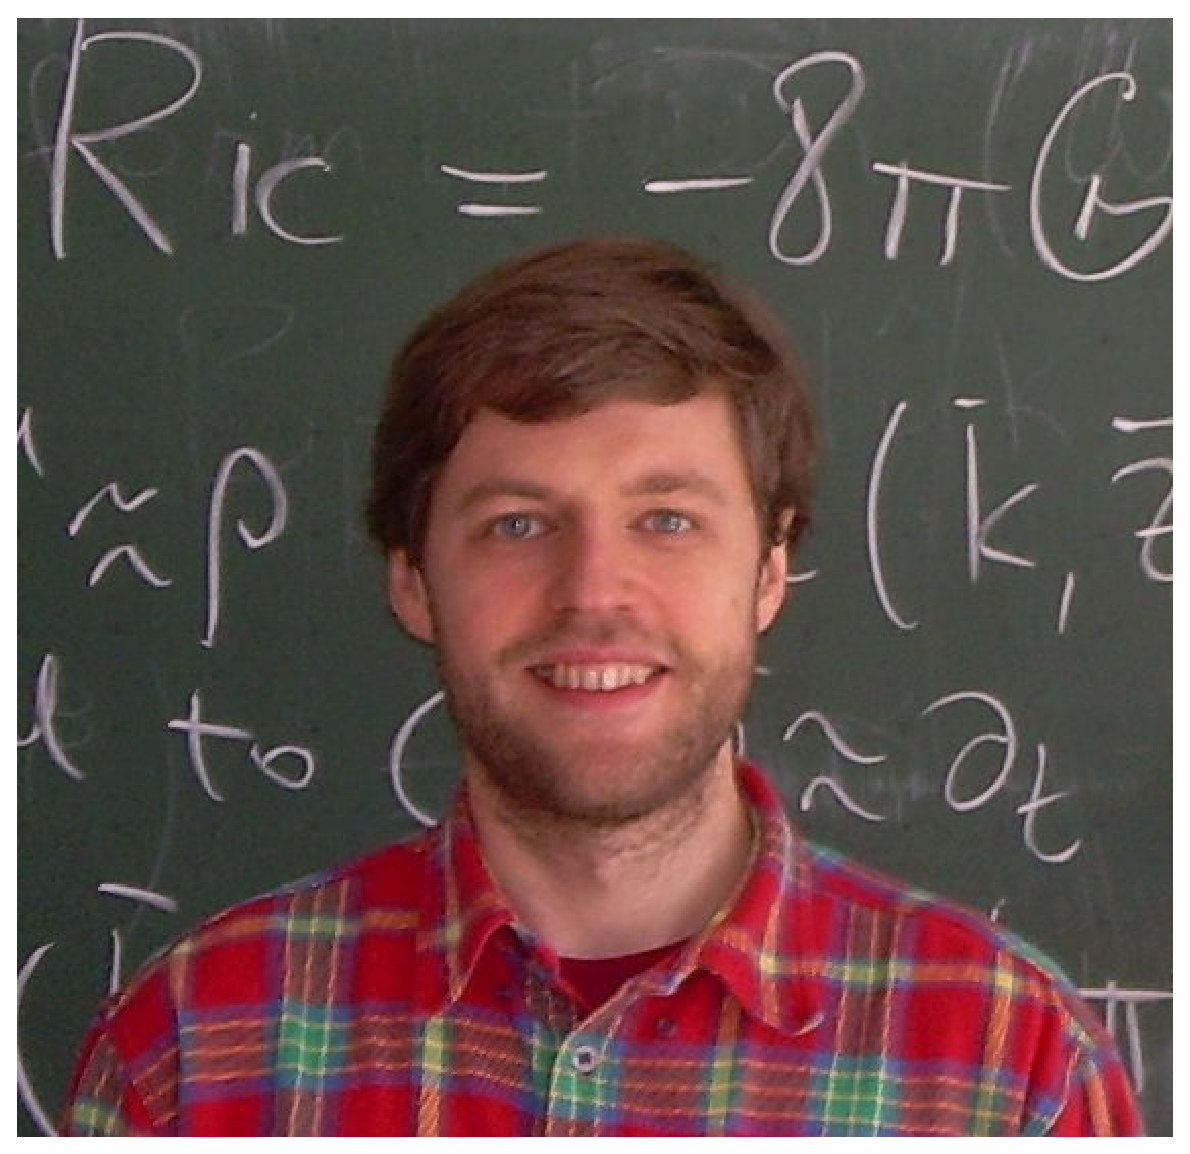
\includegraphics[width=3.2cm]{Sergei_Winitzki_blackboard_2008}%
\end{minipage}~ ~%
\begin{minipage}[t]{4cm}%
{\small{}Sergei Winitzki received a PhD in theoretical physics from
Tufts University, USA (1997) and has been a researcher and part-time
lecturer at universities in the USA, UK, and Germany. Dr.~Winitzki~
has ~authored a}%
\end{minipage}\vspace{1mm}%
\begin{minipage}[t]{7.5cm}%
{\small{}number of research articles and two books on his main professional
interest, theoretical physics. He is presently employed as a senior
academic fellow at the Ludwig-Maximilians-University, Munich (Germany).}%
\end{minipage}\fi\thispagestyle{empty}}
\title{Linear Algebra via Exterior Products}
\author{Sergei Winitzki, Ph.D.}
\date{\relax}
\uppertitleback{\vskip 1in Linear Algebra via Exterior Products\\
Copyright (c) 2009-2020 by Sergei Winitzki, Ph.D.\\
ISBN 978-1-4092-9496-2, published by \ifwanthyperlinks \href{http://lulu.com}{\textbf{lulu.com}}
\else  \textbf{lulu.com} \fi \\
Version 1.3. Last change: \today\\
\\
{\small{}Permission is granted to copy, distribute and/or modify this
\ifthisispdffile PDF file \else  document \fi  under the terms
of the \ifwanthyperlinks \href{http://www.gnu.org/copyleft/fdl.html}{\emph{GNU Free Documentation License}},
\else  GNU Free Documentation License \fi Version 1.2 or any later
version published by the Free Software Foundation; with no Invariant
Sections, no Front-Cover Texts, and no Back-Cover Texts. A copy of
the license is included in Appendix~\ref{sec:GFDL}. This license
permits you to copy this entire book for free or to print it, and
also guarantees that future revisions of the book will remain free.
The \LaTeX{} source for this book is bundled as attachment within the
PDF file\ifthisispdffile . \else , which is available on the book's
Web site (}\texttt{\footnotesize{}http://sites.google.com/site/winitzki/}{\small{}).
\fi  The text has been formatted \ifthisismini to minimize the number
of pages. \else  to fit a typical printed softcover book.\fi }\\
}
\lowertitleback{{\small{}This book is an undergraduate-level introduction to the coordinate-free
approach in basic finite-dimen\-sion\-al linear algebra. The reader
should be already exposed to the elementary array-based formalism
of vector and matrix calculations. Throughout this book, extensive
use is made of the exterior (anti-commutative, ``wedge'') product
of vectors. The co\-or\-din\-ate-free formalism and the exterior
product, while somewhat more abstract, provide a deeper understanding
of the classical results in linear algebra. The standard properties
of determinants, the Pythagoras theorem for multidimensional volumes,
the formulas of Jacobi and Liouville, the Cayley-Hamilton theorem,
properties of Pfaffians, the Jordan canonical form, as well as some
generalizations of these results  are derived without cumbersome matrix
calculations. For the benefit of students, every result is logically
motivated and discussed. Exercises with some hints are provided.}}

\maketitle
\frontmatter\pagenumbering{roman}\tableofcontents{}

\mainmatter\pagenumbering{arabic}

\addchap{Preface}

In a first course of linear algebra, one learns the various uses of
matrices, for instance the properties of determinants, eigenvectors
and eigenvalues, and methods for solving linear equations. The required
calculations are straightforward (because, conceptually, vectors and
matrices are merely ``arrays of numbers'') if cumbersome. However,
there is a more abstract and more powerful approach: Vectors are elements
of abstract vector spaces, and matrices represent linear transformations
of vectors. This \textbf{invariant} or \textbf{coordinate-free}\index{coordinate-free approach}
approach is important in algebra and has found many applications in
science. 

The purpose of this book is to help the reader make a transition to
the abstract coordinate-free approach, and also to give a hands-on
introduction to exterior products, a powerful tool of linear algebra.
I show how the coordin\-ate-free approach together with exterior
products can be used to clarify the basic results of matrix algebra,
at the same time avoiding all the laborious matrix calculations. 

Here is a simple theorem that illustrates the advantages of the exterior
product approach. A triangle is oriented arbitrarily in three-dim\-en\-sion\-al
space; the three orthogonal projections of this triangle are triangles
in the three coordinate planes. Let $S$ be the area of the initial
triangle, and let $A,B,C$ be the areas of the three projections.
Then 
\[
S^{2}=A^{2}+B^{2}+C^{2}.
\]
If one uses bivectors to represent the oriented areas of the triangle
and of its three projections, the statement above is equivalent to
the Pythagoras theorem in the space of bivectors, and the proof requires
only a few straightforward definitions and checks. A generalization
of this result to volumes of $k$-dim\-en\-sion\-al bodies embedded
in $N$-dim\-en\-sion\-al spaces is then obtained with no extra
work. I hope that the readers will appreciate the beauty of an approach
to linear algebra that allows us to obtain such results quickly and
almost without calculations.

The exterior product is widely used in connection with $n$-forms,
which are exterior products of \emph{covectors}. In this book I do
not use $n$-forms --- instead I use vectors, $n$-vectors, and their
exterior products. This approach allows a more straightforward geometric
interpretation and also simplifies calculations and proofs.

To make the book logically self-contained, I present a proof of every
basic result of linear algebra. The emphasis is not on computational
techniques, although the coordinate-free approach \emph{does} make
many computations easier and more elegant.\footnote{\textbf{Elegant}\index{elegance} means shorter and easier to remember.
Usually, \textbf{elegant} derivations are those in which some powerful
basic idea is exploited to obtain the result quickly.} The main topics covered are tensor products; exterior products; coordinate-free
definitions of the determinant $\det\hat{A}$, the trace $\textrm{Tr}\hat{A}$,
and the characteristic polynomial $Q_{\hat{A}}\left(\lambda\right)$;
basic properties of determinants; solution of linear equations, including
over-determined or under-determined systems, using Kramer's rule;
the Liouville formula $\det\exp\hat{A}=\exp\textrm{Tr}\hat{A}$ as
an identity of formal series; the algebraic complement (cofactor)
matrix; Jacobi's formula for the variation of the determinant; variation
of the characteristic polynomial and of eigenvalue; the Cayley-Hamilton
theorem; analytic functions of operators; Jordan canonical form; construction
of projectors onto Jordan cells; Hodge star and the computation of
$k$-dimensional volumes through $k$-vectors; definition and properties
of the Pfaffian $\textrm{Pf}\hat{A}$ for antisymmetric operators
$\hat{A}$. All these standard results are derived without matrix
calculations; instead, the exterior product is used as a main computational
tool. 

This book is largely \textbf{pedagogical}, meaning that the results
are long known, and the emphasis is on a clear and self-contained,
logically motivated presentation aimed at students. Therefore, some
exercises with hints and partial solutions are included, but not references
to literature.\footnote{The approach to determinants via exterior products has been known
since at least 1880 but does not seem especially popular in textbooks,
perhaps due to the somewhat abstract nature of the tensor product.
I believe that this approach to determinants and to other results
in linear algebra deserves to be more widely appreciated.} I have tried to avoid being overly pedantic while keeping the exposition
mathematically rigorous.

Sections marked with a star $^{*}$ are not especially difficult but
contain material that may be skipped at first reading. (Exercises
marked with a star \emph{are} more difficult.)

The first chapter is an introduction to the invariant approach to
vector spaces. I assume that readers are familiar with elementary
linear algebra in the language of row/column vectors and matrices;
Appendix~\ref{sec:Matrices} contains a brief overview of that material.
Good introductory books (which I did not read in detail but which
have a certain overlap with the present notes) are ``Finite-dimen\-sion\-al
Vector Spaces'' by P.~Halmos and ``Linear Algebra'' by J.~Hefferon
(the latter is a free book).

I started thinking about the approach to linear algebra based on exterior
products while still a student. I am especially grateful to Sergei
Arkhipov, Leonid Positselsky, and Arkady Vaintrob who have stimulated
my interest at that time and taught me much of what I could not otherwise
learn about algebra. Thanks are also due to Prof.~Howard Haber (UCSC)
for constructive feedback on an earlier version of this text.

In the first 10 years since I made this book available for free, many
readers sent me corrections to the text. For that, I thank Gabriel
Aguirre, Pablo Dominguez, Joseph Ferrara, Andrew J.~Ho, Yuxi Liu,
Christophe Louargant, Jiri Matousek, Dmitri Pavlov, and Michele Zaffalon.
Version~1.3 (prepared in June 2020) incorporates these corrections.

\mainmatter\pagenumbering{arabic}

\setcounter{chapter}{-1}

\chapter{Introduction and summary}

All the notions mentioned in this section will be explained below.
If you already know the definition of tensor and exterior products
and are familiar with statements such as $\textrm{End }V\cong V\otimes V^{*}$,
you may skip to Chapter ~\ref{sec:Exterior-product}. 

\section{Notation}

The following conventions are used throughout this text. 

I use the \textbf{bold emphasis} to define a new word, term, or notion,
and the definition always appears near the boldface text (whether
or not I write the word ``Definition'').

Ordered sets are denoted by round parentheses, e.g.~$\left(1,2,3\right)$.
Unordered sets are denoted using the curly parentheses, e.g.~$\left\{ a,b,c\right\} $.

The symbol $\equiv$ means ``is now being defined as'' or ``equals
by a previously given definition.'' 

The symbol ${\lyxbuildrel!\above=}$ means ``as we already know,
equals.''

A set consisting of all elements $x$ satisfying some property $P(x)$
is denoted by $\left\{ \,x\,|\,P(x)\,\text{is true }\right\} $.

A map $f$ from a set $V$ to $W$ is denoted by $f:V\rightarrow W$.
An element $v\in V$ is then mapped to an element $w\in W$, which
is written as $f:v\mapsto w$ or $f(v)=w$.

The sets of rational numbers, real numbers, and complex numbers are
denoted respectively by $\mathbb{Q}$, $\mathbb{R}$, and $\mathbb{C}$.

Statements, Lemmas, Theorems, Examples, and Exercises are numbered
only within a single subsection, so references are always to a certain
statement in a certain subsection.\footnote{I was too lazy to implement a comprehensive system of numbering for
all these items.} A reference to ``Theorem~\ref{subsec:Dimension-of-V}'' means
the unnumbered theorem in Sec.~\ref{subsec:Dimension-of-V}. 

Proofs, solutions, examples, and exercises are separated from the
rest by the symbol $\blacksquare$. More precisely, this symbol means
``I have finished with this; now we look at something else.''

$V$ is a finite-dimen\-sion\-al \textbf{vector} \textbf{space}
over a \textbf{field} $\mathbb{K}$. Vectors from $V$ are denoted
by boldface lowercase letters, e.g.~$\mathbf{v}\in V$. The \textbf{dimension}
of $V$ is $N\equiv\dim V$. 

The standard $N$-dimen\-sion\-al space over real numbers (the space
consisting of $N$-tuples of real numbers) is denoted by $\mathbb{R}^{N}$.

The \textbf{subspace spanned by} a given set of vectors $\left\{ \mathbf{v}_{1},...,\mathbf{v}_{n}\right\} $
is denoted by $\text{Span}\left\{ \mathbf{v}_{1},...,\mathbf{v}_{n}\right\} $. 

The vector space \textbf{dual} to $V$ is $V^{*}$. Elements of $V^{*}$
(\textbf{covectors}) are denoted by starred letters, e.g.~$\mathbf{f}^{*}\in V^{*}$.
A covector $\mathbf{f}^{*}$ acts on a vector $\mathbf{v}$ and produces
a number $\mathbf{f}^{*}(\mathbf{v})$.

The space of linear maps (\textbf{homomorphisms}) $V\rightarrow W$
is $\textrm{Hom}\left(V,W\right)$. The space of \textbf{linear operators}
(also called \textbf{endomorphisms}) of a vector space $V$, i.e.~the
space of all linear maps $V\rightarrow V$, is $\textrm{End }V$.
Operators are denoted by the circumflex accent, e.g.~$\hat{A}$.
The \textbf{identity} operator on $V$ is $\hat{1}_{V}\in\textrm{End }V$
(sometimes also denoted $\hat{1}$ for brevity).

The \textbf{direct} \textbf{sum} of spaces $V$ and $W$ is $V\oplus W$.
The \textbf{tensor} \textbf{product} of spaces $V$ and $W$ is $V\otimes W$.
The \textbf{exterior} (\textbf{anti-commutative}) \textbf{product}
of $V$ and $V$ is $V\!\wedge\!V$. The exterior product of $n$
copies of $V$ is $\wedge^{n}V$. \textbf{Canonical} \textbf{isomorphisms}
of vector spaces are denoted by the symbol $\cong$; for example,
$\textrm{End }V\cong V\otimes V^{*}$.

The \textbf{scalar product} of vectors is denoted by $\left\langle \mathbf{u},\mathbf{v}\right\rangle $.
The notation $\mathbf{a}\times\mathbf{b}$ is used \emph{only} for
the traditional \textbf{vector product} (also called \textbf{cross
product}) in 3-dimen\-sion\-al space. Otherwise, the product symbol
$\times$ is used to denote the continuation a long expression that
is being split between lines.

The \textbf{exterior} (\textbf{wedge}) product of vectors is denoted
by $\mathbf{a}\wedge\mathbf{b}\in\wedge^{2}V$. 

Any two nonzero tensors $\mathbf{a}_{1}\wedge...\wedge\mathbf{a}_{N}$
and $\mathbf{b}_{1}\wedge...\wedge\mathbf{b}_{N}$ in an $N$-dimensional
space are proportional to each other, say
\[
\mathbf{a}_{1}\wedge...\wedge\mathbf{a}_{N}=\lambda\mathbf{b}_{1}\wedge...\wedge\mathbf{b}_{N}.
\]
 It is then convenient to denote $\lambda$ by the ``tensor ratio''
\[
\lambda\equiv\frac{\mathbf{a}_{1}\wedge...\wedge\mathbf{a}_{N}}{\mathbf{b}_{1}\wedge...\wedge\mathbf{b}_{N}}.
\]

The number of unordered choices of $k$ items from $n$ is denoted
by 
\[
{n \choose k}=\frac{n!}{k!(n-k)!}.
\]

The $k$-linear action of a linear operator $\hat{A}$ in the space
$\wedge^{n}V$ is denoted by $\wedge^{n}\hat{A}^{k}$. (Here $0\leq k\leq n\leq N$.)
For example,
\begin{align*}
(\wedge^{3}\hat{A}^{2})\mathbf{a}\wedge\mathbf{b}\wedge\mathbf{c} & \equiv\hat{A}\mathbf{a}\wedge\hat{A}\mathbf{b}\wedge\mathbf{c}+\hat{A}\mathbf{a}\wedge\mathbf{b}\wedge\hat{A}\mathbf{c}\\
 & +\mathbf{a}\wedge\hat{A}\mathbf{b}\wedge\hat{A}\mathbf{c}.
\end{align*}

The imaginary unit ($\sqrt{-1}$) is denoted by a \emph{roman} ``$\text{i}$,''
while the base of natural logarithms is written as an \emph{italic}
``$e$.'' For example, I would write $e^{\text{i}\pi}=-1$. This
convention is designed to avoid conflicts with the much used index
$i$ and with labeled vectors such as $\mathbf{e}_{i}$.

I write an italic $d$ in the derivatives, such as $df/dx$, and in
integrals, such as $\int f(x)dx$, because in these cases the symbols
$dx$ do not refer to a separate well-defined object ``$dx$'' but
are a part of the traditional symbolic notation used in calculus.
Differential forms (or, for that matter, nonstandard calculus) \emph{do}
make ``$\text{d}x$'' into a well-defined object; in that case I
write a roman ``d'' in ``$\text{d}x$.'' Neither calculus nor
differential forms are actually used in this book; the only exception
is the occasional use of the derivative $d/dx$ applied to polynomials
in $x$. I will not need to make a distinction between $d/dx$ and
$\partial/\partial x$; the derivative of a function $f$ with respect
to $x$ is denoted by $\partial_{x}f$.

\section{Sample quiz problems}

The following problems can be solved using techniques explained in
this book. (These problems are of varying difficulty.) In these problems
$V$ is an $N$-dimen\-sion\-al vector space (with a scalar product
if indicated).

\paragraph{Exterior multiplication:}

If two tensors $\omega_{1},\omega_{2}\in\wedge^{k}V$ (with $1\leq k\leq N-1$)
are such that $\omega_{1}\wedge\mathbf{v}=\omega_{2}\wedge\mathbf{v}$
for \emph{all} vectors $\mathbf{v}\in V$, show that $\omega_{1}=\omega_{2}$.

\paragraph{Insertions:}

a) It is given that $\psi\in\wedge^{k}V$ (with $1\leq k\leq N-1$)
and $\psi\wedge\mathbf{a}=0$, where $\mathbf{a}\in V$ and $\mathbf{a}\neq0$.
Further, a covector $\mathbf{f}^{*}\in V^{*}$ is given such that
$\mathbf{f}^{*}(\mathbf{a})\neq0$. Show that 
\[
\psi=\frac{1}{\mathbf{f}^{*}(\mathbf{a})}\mathbf{a}\wedge(\iota_{\mathbf{f}^{*}}\psi).
\]

b) It is given that $\psi\wedge\mathbf{a}=0$ and $\psi\wedge\mathbf{b}=0$,
where $\psi\in\wedge^{k}V$ (with $2\leq k\leq N-1$) and $\mathbf{a},\mathbf{b}\in V$
such that $\mathbf{a}\wedge\mathbf{b}\neq0$. Show that there exists
$\chi\in\wedge^{k-2}V$ such that $\psi=\mathbf{a}\wedge\mathbf{b}\wedge\chi$. 

c) It is given that $\psi\wedge\mathbf{a}\wedge\mathbf{b}=0$, where
$\psi\in\wedge^{k}V$ (with $2\leq k\leq N-2$) and $\mathbf{a},\mathbf{b}\in V$
such that $\mathbf{a}\wedge\mathbf{b}\neq0$. Is it always true that
$\psi=\mathbf{a}\wedge\mathbf{b}\wedge\chi$ for some $\chi\in\wedge^{k-2}V$?

\paragraph{Determinants:}

a) Suppose $\hat{A}$ is a linear operator defined by $\hat{A}=\sum_{i=1}^{N}\mathbf{a}_{i}\otimes\mathbf{b}_{i}^{*}$,
where $\mathbf{a}_{i}\in V$ are given vectors and $\mathbf{b}_{i}\in V^{*}$
are given covectors; $N=\dim V$. Show that 
\[
\det\hat{A}=\frac{\mathbf{a}_{1}\wedge...\wedge\mathbf{a}_{N}}{\mathbf{e}_{1}\wedge...\wedge\mathbf{e}_{N}}\,\frac{\mathbf{b}_{1}^{*}\wedge...\wedge\mathbf{b}_{N}^{*}}{\mathbf{e}_{1}^{*}\wedge...\wedge\mathbf{e}_{N}^{*}},
\]
where $\left\{ \mathbf{e}_{j}\right\} $ is an arbitrary basis and
$\left\{ \mathbf{e}_{j}^{*}\right\} $ is the corresponding dual basis.
Show that the expression above is independent of the choice of the
basis $\left\{ \mathbf{e}_{j}\right\} $.

b) Suppose that a scalar product is given in $V$, and an operator
$\hat{A}$ is defined by 
\[
\hat{A}\mathbf{x}\equiv\sum_{i=1}^{N}\mathbf{a}_{i}\left\langle \mathbf{b}_{i},\mathbf{x}\right\rangle .
\]
Further, suppose that $\left\{ \mathbf{e}_{j}\right\} $ is an orthonormal
basis in $V$. Show that
\[
\det\hat{A}=\frac{\mathbf{a}_{1}\wedge...\wedge\mathbf{a}_{N}}{\mathbf{e}_{1}\wedge...\wedge\mathbf{e}_{N}}\,\frac{\mathbf{b}_{1}\wedge...\wedge\mathbf{b}_{N}}{\mathbf{e}_{1}\wedge...\wedge\mathbf{e}_{N}},
\]
and that this expression is independent of the choice of the orthonormal
basis $\left\{ \mathbf{e}_{j}\right\} $ and of the orientation of
the basis.

\paragraph{Hyperplanes:}

a) Let us suppose that the ``price'' of the vector $\mathbf{x}\in V$
is given by the formula 
\[
\text{Cost}\left(\mathbf{x}\right)\equiv C(\mathbf{x},\mathbf{x}),
\]
where $C(\mathbf{a},\mathbf{b})$ is a known, positive-definite bilinear
form. Determine the ``cheapest'' vector $\mathbf{x}$ belonging
to the affine hyperplane $\mathbf{a}^{*}(\mathbf{x})=\alpha$, where
$\mathbf{a}^{*}\in V^{*}$ is a nonzero covector and $\alpha$ is
a number.\index{hyperplane}

b) We are now working in a vector space with a scalar product, and
the ``price'' of a vector $\mathbf{x}$ is $\left\langle \mathbf{x},\mathbf{x}\right\rangle $.
Two affine hyperplanes are given by equations $\left\langle \mathbf{a},\mathbf{x}\right\rangle =\alpha$
and $\left\langle \mathbf{b},\mathbf{x}\right\rangle =\beta$, where
$\mathbf{a}$ and $\mathbf{b}$ are given vectors, $\alpha$ and $\beta$
are numbers, and $\mathbf{x}\in V$. (It is assured that $\mathbf{a}$
and $\mathbf{b}$ are nonzero and not parallel to each other.) Determine
the ``cheapest'' vector $\mathbf{x}$ belonging to the intersection
of the two hyperplanes.

\paragraph{Too few equations:}

A linear operator $\hat{A}$ is defined by $\hat{A}=\sum_{i=1}^{k}\mathbf{a}_{i}\otimes\mathbf{b}_{i}^{*}$,
where $\mathbf{a}_{i}\in V$ are given vectors and $\mathbf{b}_{i}^{*}\in V^{*}$
are given covectors, and $k<N=\dim V$. Show that the vector equation
$\hat{A}\mathbf{x}=\mathbf{c}$ has no solutions if $\mathbf{a}_{1}\wedge...\wedge\mathbf{a}_{k}\wedge\mathbf{c}\neq0$.
In case $\mathbf{a}_{1}\wedge...\wedge\mathbf{a}_{k}\wedge\mathbf{c}=0$,
show that solutions $\mathbf{x}$ surely exist when $\mathbf{b}_{1}^{*}\wedge...\wedge\mathbf{b}_{k}^{*}\neq0$
but may not exist otherwise.

\paragraph{Operator functions:}

It is known that the operator $\hat{A}$ satisfies the operator equation
$\hat{A}^{2}=-\hat{1}$. Simplify the oper\-ator-valued functions
$\frac{1+\hat{A}}{3-\hat{A}}$, $\cos(\lambda\hat{A})$, and $\sqrt{\hat{A}+2}$
to linear formulas involving $\hat{A}$. (Here $\lambda$ is a number,
while the numbers $1$, $2$, $3$ stand for multiples of the identity
operator.) Compare the results with the complex numbers $\frac{1+\text{i}}{3-\text{i}}$,
$\cos(\lambda\text{i})$, $\sqrt{\text{i}+2}$ and generalize the
conclusion to a theorem about computing analytic functions $f(\hat{A})$.

\paragraph{Inverse operator:}

It is known that $\hat{A}\hat{B}=\lambda\hat{1}_{V}$, where $\lambda\neq0$
is a number. Prove that also $\hat{B}\hat{A}=\lambda\hat{1}_{V}$.
(Both $\hat{A}$ and $\hat{B}$ are linear operators in a fin\-ite-dimen\-sion\-al
space $V$.)

\paragraph{Trace and determinant: }

Consider the space of polynomials in the variables $x$ and $y$,
where we admit only polynomials of the form $a_{0}+a_{1}x+a_{2}y+a_{3}xy$
(with $a_{j}\in\mathbb{R}$). An operator $\hat{A}$ is defined by
\[
\hat{A}\equiv x\frac{\partial}{\partial x}-\frac{\partial}{\partial y}.
\]
Show that $\hat{A}$ is a linear operator in this space. Compute the
trace and the determinant of $\hat{A}$. If $\hat{A}$ is invertible,
compute $\hat{A}^{-1}(x+y)$.

\paragraph{Cayley-Hamilton theorem:}

Express $\det\hat{A}$ through $\text{Tr}\hat{A}$ and $\text{Tr}(\hat{A}^{2})$
for an arbitrary operator $\hat{A}$ in a \emph{two}-dimen\-sion\-al
space.

\paragraph{Algebraic complement:}

Let $\hat{A}$ be a linear operator and $\tilde{\hat{A}}$ its algebraic
complement. 

a) Show that 
\[
\text{Tr}\tilde{\hat{A}}=\wedge^{N}\hat{A}^{N-1}.
\]
Here $\wedge^{N}\hat{A}^{N-1}$ is the coefficient at $(-\lambda)$
in the characteristic polynomial of $\hat{A}$ (that is, minus the
coefficient preceding the determinant).

b) For $t$-independent operators $\hat{A}$ and $\hat{B}$, show
that
\[
\frac{\partial}{\partial t}\det(\hat{A}+t\hat{B})=\text{Tr}(\tilde{\hat{A}}\hat{B}).
\]


\paragraph{Liouville formula:}

Suppose $\hat{X}(t)$ is a defined as solution of the differential
equation
\[
\partial_{t}\hat{X}(t)=\hat{A}(t)\hat{X}(t)-\hat{X}(t)\hat{A}(t),
\]
where $\hat{A}(t)$ is a given operator. (Operators that are functions
of $t$ can be understood as oper\-ator-valued formal power series.) 

a) Show that the determinant of $\hat{X}(t)$ is independent of $t$. 

b) Show that all the coefficients of the characteristic polynomial
of $\hat{X}(t)$ are independent of $t$.

\paragraph{Hodge star:}

Suppose $\left\{ \mathbf{v}_{1},...,\mathbf{v}_{N}\right\} $ is a
basis in $V$, not necessarily orthonormal, while $\left\{ \mathbf{e}_{j}\right\} $
is a positively oriented orthonormal basis. Show that 
\[
*(\mathbf{v}_{1}\wedge...\wedge\mathbf{v}_{N})=\frac{\mathbf{v}_{1}\wedge...\wedge\mathbf{v}_{N}}{\mathbf{e}_{1}\wedge...\wedge\mathbf{e}_{N}}.
\]


\paragraph{Volume in space:}

Consider the space of polynomials of degree at most 4 in the variable
$x$. The scalar product of two polynomials $p_{1}(x)$ and $p_{2}(x)$
is defined by
\[
\left\langle p_{1},p_{2}\right\rangle \equiv\frac{1}{2}\int_{-1}^{1}p_{1}(x)p_{2}(x)dx.
\]
Determine the three-dimensional volume of the tetrahedron with vertices
at the ``points'' $0$, $1+x$, $x^{2}+x^{3}$, $x^{4}$ in this
five-dimen\-sion\-al space.

\section{A list of results}

Here is a list of some results explained in this book. If you already
know all these results and their derivations, you may not need to
read any further.

Vector spaces may be defined over an abstract number field, without
specifying the number of dimensions or a basis.

The set $\left\{ a+b\sqrt{41}\,|\,a,b\in\mathbb{Q}\right\} $ is a
number field.

Any vector can be represented as a linear combination of basis vectors.
All bases have equally many vectors.

The set of all linear maps from one vector space to another is denoted
$\text{Hom}(V,W)$ and is a vector space.

The zero vector is not an eigenvector (by definition).

An operator having in some basis the matrix representation $\left(\begin{array}{cc}
0 & 1\\
0 & 0
\end{array}\right)$ cannot be diagonalized.

The dual vector space $V^{*}$ has the same dimension as $V$ (for
finite-dimen\-sion\-al spaces).

Given a nonzero covector $\mathbf{f}^{*}\in V^{*}$, the set of vectors
$\mathbf{v}\in V$ such that $\mathbf{f}^{*}(\mathbf{v})=0$ is a
subspace of codimension 1 (a hyperplane).

The tensor product of $\mathbb{R}^{m}$ and $\mathbb{R}^{n}$ has
dimension $mn$.

Any linear map $\hat{A}:V\rightarrow W$ can be represented by a tensor
of the form $\sum_{i=1}^{k}\mathbf{v}_{i}^{*}\otimes\mathbf{w}_{i}\in V^{*}\otimes W$.
The rank of $\hat{A}$ is equal to the smallest number of simple tensor
product terms $\mathbf{v}_{i}^{*}\otimes\mathbf{w}_{i}$ required
for this representation.

The identity map $\hat{1}_{V}:V\rightarrow V$ is represented as the
tensor $\sum_{i=1}^{N}\mathbf{e}_{i}^{*}\otimes\mathbf{e}_{i}\in V^{*}\otimes V$,
where $\left\{ \mathbf{e}_{i}\right\} $ is any basis and $\left\{ \mathbf{e}_{i}^{*}\right\} $
its dual basis. This tensor does not depend on the choice of the basis
$\left\{ \mathbf{e}_{i}\right\} $.

A set of vectors $\left\{ \mathbf{v}_{1},...,\mathbf{v}_{k}\right\} $
is linearly independent if and only if $\mathbf{v}_{1}\wedge...\wedge\mathbf{v}_{k}\neq0$.
If $\mathbf{v}_{1}\wedge...\wedge\mathbf{v}_{k}\neq0$ but $\mathbf{v}_{1}\wedge...\wedge\mathbf{v}_{k}\wedge\mathbf{x}=0$
then the vector $\mathbf{x}$ belongs to the subspace $\text{Span}\left\{ \mathbf{v}_{1},...,\mathbf{v}_{k}\right\} $.

The dimension of the space $\wedge^{k}V$ is ${N \choose k}$, where
$N\equiv\dim V$.

Insertion $\iota_{\mathbf{a}^{*}}\omega$ of a covector $\mathbf{a}^{*}\in V^{*}$
into an antisymmetric tensor $\omega\in\wedge^{k}V$ has the property
\[
\mathbf{v}\wedge(\iota_{\mathbf{a}^{*}}\omega)+\iota_{\mathbf{a}^{*}}(\mathbf{v}\wedge\omega)=\mathbf{a}^{*}(\mathbf{v})\omega.
\]

Given a basis $\left\{ \mathbf{e}_{i}\right\} $, the dual basis $\left\{ \mathbf{e}_{i}^{*}\right\} $
may be computed as
\[
\mathbf{e}_{i}^{*}(\mathbf{x})=\frac{\mathbf{e}_{1}\wedge...\wedge\mathbf{x}\wedge...\wedge\mathbf{e}_{N}}{\mathbf{e}_{1}\wedge...\wedge\mathbf{e}_{N}},
\]
where $\mathbf{x}$ replaces $\mathbf{e}_{i}$ in the numerator.

The subspace spanned by a set of vectors $\left\{ \mathbf{v}_{1},...,\mathbf{v}_{k}\right\} $,
not necessarily linearly independent, can be characterized by a certain
antisymmetric tensor $\omega$, which is the exterior product of the
largest number of $\mathbf{v}_{i}$'s such that $\omega\neq0$. The
tensor $\omega$, computed in this way, is unique up to a constant
factor.

The $n$-vector (antisymmetric tensor) $\mathbf{v}_{1}\wedge...\wedge\mathbf{v}_{n}$
represents geometrically the oriented $n$-dimen\-sion\-al volume
of the parallelepiped spanned by the vectors $\mathbf{v}_{i}$.

The determinant of a linear operator $\hat{A}$ is the coefficient
that multiplies the oriented volume of any parallelepiped transformed
by $\hat{A}$. In our notation, the operator $\wedge^{N}\hat{A}^{N}$
acts in $\wedge^{N}V$ as multiplication by $\det\hat{A}$.

If each of the given vectors $\{\mathbf{v}{}_{1},...,\mathbf{v}_{N}\}$
is expressed through a basis $\left\{ \mathbf{e}_{i}\right\} $ as
$\mathbf{v}_{j}=\sum_{i=1}^{N}v_{ij}\mathbf{e}_{i}$, the determinant
of the matrix $v_{ij}$ is found as 
\[
\det(v_{ij})=\det(v_{ji})=\frac{\mathbf{v}_{1}\wedge...\wedge\mathbf{v}_{N}}{\mathbf{e}_{1}\wedge...\wedge\mathbf{e}_{N}}.
\]

A linear operator $\hat{A}:V\rightarrow V$ and its canonically defined
transpose $\hat{A}^{T}:V^{*}\rightarrow V^{*}$ have the same characteristic
polynomials.

If $\det\hat{A}\neq0$ then the inverse operator $\hat{A}^{-1}$ exists,
and a linear equation $\hat{A}\mathbf{x}=\mathbf{b}$ has the unique
solution $\mathbf{x}=\hat{A}^{-1}\mathbf{b}$. Otherwise, solutions
exist if $\mathbf{b}$ belongs to the image of $\hat{A}$. Explicit
solutions may be constructed using Kramer's rule: If a vector $\mathbf{b}$
belongs to the subspace spanned by vectors $\left\{ \mathbf{v}_{1},...,\mathbf{v}_{n}\right\} $
then $\mathbf{b}=\sum_{i=1}^{n}b$$_{i}\mathbf{v}_{i}$, where the
coefficients $\mathbf{b}_{i}$ may be found (assuming $\mathbf{v}_{1}\wedge...\wedge\mathbf{v}_{n}\neq0$)
as
\[
b_{i}=\frac{\mathbf{v}_{1}\wedge...\wedge\mathbf{x}\wedge...\wedge\mathbf{v}_{n}}{\mathbf{v}_{1}\wedge...\wedge\mathbf{v}_{n}}
\]
(here $\mathbf{x}$ replaces $\mathbf{v}_{i}$ in the exterior product
in the numerator).

Eigenvalues of a linear operator are roots of its characteristic polynomial.
For each root $\lambda_{i}$, there exists at least one eigenvector
corresponding to the eigenvalue $\lambda_{i}$. 

If $\left\{ \mathbf{v}_{1},...,\mathbf{v}_{k}\right\} $ are eigenvectors
corresponding to \emph{all different} eigenvalues $\lambda_{1},...,\lambda_{k}$
of some operator, then the set $\left\{ \mathbf{v}_{1},...,\mathbf{v}_{k}\right\} $
is linearly independent.

The dimension of the eigenspace corresponding to $\lambda_{i}$ is
not larger than the algebraic multiplicity of the root $\lambda_{i}$
in the characteristic polynomial.

\emph{(Below in this section we always denote by $N$ the dimension
of the space $V$.)}

The trace of an operator $\hat{A}$ can be expressed as $\wedge^{N}\hat{A}^{1}$. 

We have $\text{Tr}(\hat{A}\hat{B})=\mbox{\text{Tr}}(\hat{B}\hat{A})$.
This holds even if $\hat{A},\hat{B}$ are maps between different spaces,
i.e.~$\hat{A}:V\rightarrow W$ and $\hat{B}:W\rightarrow V$.

If an operator $\hat{A}$ is nilpotent, its characteristic polynomial
is $\left(-\lambda\right)^{N}$, i.e.~the same as the characteristic
polynomial of a zero operator.

The $j$-th coefficient of the characteristic polynomial of $\hat{A}$
is $\left(-1\right)^{j}(\wedge^{N}\hat{A}^{j})$.

Each coefficient of the characteristic polynomial of $\hat{A}$ can
be expressed as a polynomial function of $N$ traces of the form $\text{Tr}(\hat{A}^{k})$,
$k=1,...,N$.

The space $\wedge^{N-1}V$ is $N$-dimen\-sion\-al like $V$ itself,
and there is a canonical isomorphism between $\text{End}(\wedge^{N-1}V)$
and $\text{End}(V)$. This isomorphism, called \textbf{exterior} \textbf{transposition}\index{exterior transposition},
is denoted by $(...)^{\wedge T}$. The exterior transpose of an operator
$\hat{X}\in\text{End}\,V$ is defined by 
\[
(\hat{X}^{\wedge T}\omega)\wedge\mathbf{v}\equiv\omega\wedge\hat{X}\mathbf{v},\quad\forall\omega\in\wedge^{N-1}V,\:\mathbf{v}\in V.
\]
Similarly, one defines the exterior transposition map between $\text{End}(\wedge^{N-k}V)$
and $\text{End}(\wedge^{k}V)$ for all $k=1,...,N$.

The algebraic complement operator (normally defined as a matrix consisting
of minors) is canonically defined through exterior transposition as
$\tilde{\hat{A}}\equiv({\wedge^{N-1}\hat{A}^{N-1}})^{\wedge T}$.
It can be expressed as a polynomial in $\hat{A}$ and satisfies the
identity $\tilde{\hat{A}}\hat{A}=(\det\hat{A})\hat{1}_{V}$. Also,
all other operators
\[
\hat{A}_{(k)}\equiv\big({\wedge^{N-1}\hat{A}^{N-k}}\big)^{\wedge T},\quad k=1,...,N
\]
can be expressed as polynomials in $\hat{A}$ with known coefficients.

The characteristic polynomial of $\hat{A}$ gives the zero operator
if applied to the operator $\hat{A}$ (the Cayley-Ham\-il\-ton theorem).
A similar theorem holds for each of the operators $\wedge^{k}\hat{A}^{1}$,
$2\leq k\leq N-1$ (with different polynomials).

A formal power series $f(t)$ can be applied to the operator $t\hat{A}$;
the result is an oper\-ator-valued formal series $f(t\hat{A})$ that
has the usual properties, e.g.
\[
\partial_{t}f(t\hat{A})=\hat{A}f^{\prime}(t\hat{A}).
\]

If $\hat{A}$ is diagonalized with eigenvalues $\left\{ \lambda_{i}\right\} $
in the eigenbasis $\left\{ \mathbf{e}_{i}\right\} $, then a formal
power series $f(t\hat{A})$ is diagonalized in the same basis with
eigenvalues $f(t\lambda_{i})$.

If an operator $\hat{A}$ satisfies a polynomial equation such as
$p(\hat{A})=0$, where $p(x)$ is a known polynomial of degree $k$
(not necessarily, but possibly, the characteristic polynomial of $\hat{A}$)
then any formal power series $f(t\hat{A})$ is reduced to a polynomial
in $t\hat{A}$ of degree not larger than $k-1$. This polynomial can
be computed as the interpolating polynomial for the function $f(tx)$
at points $x=x_{i}$ where $x_{i}$ are the (all different) roots
of $p(x)$. Suitable modifications are available when \emph{not all}
roots are different. So one can compute any analytic function $f(\hat{A})$
of the operator $\hat{A}$ as long as one knows a polynomial equation
satisfied by $\hat{A}$. 

A square root of an operator $\hat{A}$ (i.e.~a linear operator $\hat{B}$
such that $\hat{B}\hat{B}=\hat{A}$) is not unique and does not always
exist. In two and three dimensions, one can either obtain all square
roots explicitly as polynomials in $\hat{A}$, or determine that some
square roots are not expressible as polynomials in $\hat{A}$ or that
square roots of $\hat{A}$ do not exist at all. 

If an operator $\hat{A}$ depends on a parameter $t$, one can express
the derivative of the determinant of $\hat{A}$ through the algebraic
complement $\tilde{\hat{A}}$ (Jacobi's formula),
\[
\partial_{t}\det\hat{A}(t)=\text{Tr}(\tilde{\hat{A}}\partial_{t}\hat{A}).
\]
Derivatives of other coefficients $q_{k}\equiv\wedge^{N}\hat{A}^{N-k}$
of the characteristic polynomial are given by similar formulas, 
\[
\partial_{t}q_{k}=\text{Tr}\,\big[(\wedge^{N-1}\hat{A}^{N-k-1})^{\wedge T}\partial_{t}\hat{A}\big].
\]

The Liouville formula holds: $\det\exp\hat{A}=\exp\text{Tr}\hat{A}$.

Any operator (not necessarily diagonalizable) can be reduced to a
Jordan canonical form in a Jordan basis. The Jordan basis consists
of eigenvectors and root vectors for each eigenvalue.

Given an operator $\hat{A}$ whose characteristic polynomial is known
(hence all roots $\lambda_{i}$ and their algebraic multiplicities
$m_{i}$ are known), one can construct explicitly a projector $\hat{P}_{\lambda_{i}}$
onto a Jordan cell for any chosen eigenvalue $\lambda_{i}$. The projector
is found as a polynomial in $\hat{A}$ with known coefficients.

\emph{(Below in this section we assume that a scalar product is fixed
in $V$.)}

A nondegenerate scalar product provides a one-to-one correspondence
between vectors and covectors. Then the canonically transposed operator
$\hat{A}^{T}:V^{*}\rightarrow V^{*}$ can be mapped into an operator
in $V$, denoted also by $\hat{A}^{T}$. (This operator is represented
by the transposed matrix only in an \emph{orthonormal} basis.) We
have $(\hat{A}\hat{B})^{T}=\hat{B}^{T}\hat{A}^{T}$ and $\det(\hat{A}^{T})=\det\hat{A}$.

Orthogonal transformations have determinants equal to $\pm1$. Mirror
reflections are orthogonal transformations and have determinant equal
to $-1$.

Given an orthonormal basis $\left\{ \mathbf{e}_{i}\right\} $, one
can define the \textbf{unit volume tensor}\index{unit volume tensor}
$\omega=\mathbf{e}_{1}\wedge...\wedge\mathbf{e}_{N}$. The tensor
$\omega$ is then independent of the choice of $\left\{ \mathbf{e}_{i}\right\} $
up to a factor $\pm1$ due to the orientation of the basis (i.e.~the
ordering of the vectors of the basis), as long as the scalar product
is kept fixed.

Given a fixed scalar product $\left\langle \cdot,\cdot\right\rangle $
and a fixed orientation of space, the Hodge star operation is uniquely
defined as a linear map (isomorphism) $\wedge^{k}V\rightarrow\wedge^{N-k}V$
for each $k=0,...,N$. For instance, 
\[
*\mathbf{e}_{1}=\mathbf{e}_{2}\wedge\mathbf{e}_{3}\wedge...\wedge\mathbf{e}_{N};\quad*(\mathbf{e}_{1}\wedge\mathbf{e}_{2})=\mathbf{e}_{3}\wedge...\wedge\mathbf{e}_{N},
\]
 if $\left\{ \mathbf{e}_{i}\right\} $ is \emph{any} positively oriented,
orthonormal basis.

The Hodge star map satisfies
\[
\left\langle \mathbf{a},\mathbf{b}\right\rangle =*(\mathbf{a}\wedge*\mathbf{b})=*(\mathbf{b}\wedge*\mathbf{a}),\quad\mathbf{a},\mathbf{b}\in V.
\]

In a three-dimen\-sion\-al space, the usual vector product and triple
product can be expressed through the Hodge star as
\[
\mathbf{a}\times\mathbf{b}=*(\mathcal{\mathbf{a}\wedge\mathbf{b}}),\;\mathbf{a}\cdot(\mathbf{b}\times\mathbf{c})=*(\mathbf{a}\wedge\mathbf{b}\wedge\mathbf{c}).
\]

The volume of an $N$-dimen\-sion\-al parallelepiped spanned by
$\left\{ \mathbf{v}_{1},...,\mathbf{v}_{N}\right\} $ is equal to
$\sqrt{\det(G_{ij})}$, where $G_{ij}\equiv\left\langle \mathbf{v}_{i},\mathbf{v}_{j}\right\rangle $
is the matrix of the pairwise scalar products.

Given a scalar product in $V$, a scalar product is canonically defined
also in the spaces $\wedge^{k}V$ for all $k=2,...,N$. This scalar
product can be defined by 
\[
\left\langle \omega_{1},\omega_{2}\right\rangle =*(\omega_{1}\wedge*\omega_{2})=*(\omega_{2}\wedge*\omega_{1})=\left\langle \omega_{2},\omega_{1}\right\rangle ,
\]
where $\omega_{1,2}\in\wedge^{k}V$. Alternatively, this scalar product
is defined by choosing an orthonormal basis $\left\{ \mathbf{e}_{j}\right\} $
and postulating that $\mathbf{e}_{i_{1}}\wedge...\wedge\mathbf{e}_{i_{k}}$
is normalized and orthogonal to any other such tensor with different
indices $\left\{ i_{j}|j=1,...,k\right\} $. The $k$-dimen\-sion\-al
volume of a parallelepiped spanned by vectors $\left\{ \mathbf{v}_{1},...,\mathbf{v}_{k}\right\} $
is found as $\sqrt{\left\langle \psi,\psi\right\rangle }$ with $\psi\equiv\mathbf{v}_{1}\wedge...\wedge\mathbf{v}_{k}\in\wedge^{k}V$.

The insertion $\iota_{\mathbf{v}}\psi$ of a vector $\mathbf{v}$
into a $k$-vector $\psi\in\wedge^{k}V$ (or the ``interior product'')
can be expressed as
\[
\iota_{\mathbf{v}}\psi=*(\mathbf{v}\wedge*\psi).
\]
If $\omega\equiv\mathbf{e}_{1}\wedge...\wedge\mathbf{e}_{N}$ is the
unit volume tensor, we have $\iota_{\mathbf{v}}\omega=*\mathbf{v}$.

Symmetric, antisymmetric, Hermitian, and anti-Hermitian operators
are always diagonalizable (if we allow complex eigenvalues and eigenvectors).
Eigenvectors of these operators can be chosen orthogonal to each other. 

Antisymmetric operators are representable as elements of $\wedge^{2}V$
of the form $\sum_{i=1}^{n}\mathbf{a}_{i}\wedge\mathbf{b}_{i}$, where
one needs no more than $N/2$ terms, and the vectors $\mathbf{a}_{i}$,
$\mathbf{b}_{i}$ can be chosen mutually orthogonal to each other.
(For this, we do not need complex vectors.)

The \textbf{Pfaffian}\index{Pfaffian} of an antisymmetric operator
$\hat{A}$ in even-dimen\-sion\-al space is the number $\text{Pf}\,\hat{A}$
defined as 
\[
\frac{1}{(N/2)!}\underbrace{A\wedge...\wedge A}_{N/2}=(\text{Pf}\,\hat{A})\mathbf{e}_{1}\wedge...\wedge\mathbf{e}_{N},
\]
 where $\left\{ \mathbf{e}_{i}\right\} $ is an orthonormal basis.
Some basic properties of the Pfaffian are 
\begin{align*}
(\text{Pf }\hat{A})^{2} & =\det\hat{A},\\
\text{Pf }(\hat{B}\hat{A}\hat{B}^{T}) & =(\det\hat{B})(\text{Pf }\hat{A}),
\end{align*}
where $\hat{A}$ is an antisymmetric operator ($\hat{A}^{T}=-\hat{A}$)
and $\hat{B}$ is an arbitrary operator.

\chapter{Linear algebra without coordinates}

\section{Vector spaces}

Abstract vector spaces are developed as a generalization of the familiar
vectors in Euclidean space.

\subsection{Three-dimen\-sion\-al Euclidean geometry}

Let us begin with something you already know. Three-dimen\-sion\-al
vectors are specified by triples of coordinates, $\mathbf{r}\equiv\left(x,y,z\right)$.
The operations of \textbf{vector sum} and \textbf{vector product}
of such vectors are defined by 
\begin{align}
\left(x_{1},y_{1},z_{1}\right)+\left(x_{2},y_{2},z_{2}\right) & \equiv\left(x_{1}+x_{2},y_{1}+y_{2},z_{1}+z_{2}\right);\label{eq:3d sum}\\
\left(x_{1},y_{1},z_{1}\right)\times\left(x_{2},y_{2},z_{2}\right) & \equiv(y_{1}z_{2}-z_{1}y_{2},\,z_{1}x_{2}-x_{1}z_{2},\nonumber \\
 & x_{1}y_{2}-y_{1}x_{2}).\label{eq:3d vector product}
\end{align}
(I assume that these definitions are familiar to you.) Vectors can
be \textbf{rescaled} by multiplying them with real numbers, 
\begin{equation}
c\mathbf{r}=c\left(x,y,z\right)\equiv\left(cx,cy,cz\right).\label{eq:3d scalar mult}
\end{equation}
A rescaled vector is parallel to the original vector and points either
in the same or in the opposite direction. In addition, a \textbf{scalar
product} of two vectors is defined,
\begin{equation}
\left(x_{1},y_{1},z_{1}\right)\cdot\left(x_{2},y_{2},z_{2}\right)\equiv x_{1}x_{2}+y_{1}y_{2}+z_{1}z_{2}.\label{eq:3d scalar prod}
\end{equation}
These operations encapsulate all of Euclidean geometry in a purely
algebraic language. For example, the \textbf{length} of a vector $\mathbf{r}$
is 
\begin{equation}
\left|\mathbf{r}\right|\equiv\sqrt{\mathbf{r}\cdot\mathbf{r}}=\sqrt{x^{2}+y^{2}+z^{2}},\label{eq:r modulus}
\end{equation}
 the \textbf{angle} $\alpha$ between vectors $\mathbf{r}_{1}$ and
$\mathbf{r}_{2}$ is found from the relation (the cosine theorem)
\[
\left|\mathbf{r}_{1}\right|\left|\mathbf{r}_{2}\right|\cos\alpha=\mathbf{r}_{1}\cdot\mathbf{r}_{2},
\]
while the \textbf{area} of a triangle spanned by vectors $\mathbf{r}_{1}$
and $\mathbf{r}_{2}$ is
\[
S=\frac{1}{2}\left|\mathbf{r}_{1}\times\mathbf{r}_{2}\right|.
\]

Using these definitions, one can reformulate every geometric statement
(such as, ``a triangle having two equal sides has also two equal
angles'') in terms of relations between vectors, which are ultimately
reducible to algebraic equations involving a set of numbers. The replacement
of geometric constructions by algebraic relations is useful because
it allows us to free ourselves from the confines of our three-dimensional
intuition; we are then able to solve problems in higher-dimen\-sion\-al
spaces. The price is a greater complication of the algebraic equations
and inequalities that need to be solved. To make these equations more
transparent and easier to handle, the theory of linear algebra is
developed. The first step is to realize what features of vectors are
essential and what are just accidental facts of our familiar three-dimen\-sion\-al
Euclidean space.

\subsection{From three-dimen\-sion\-al vectors to abstract vectors}

Abstract vector spaces retain the essential properties of the familiar
Euclidean geometry but generalize it in two ways: First, the dimension
of space is not 3 but  an arbitrary integer number (or even  infinity);
second, the coordinates are ``abstract numbers'' (see below) instead
of real numbers. Let us first pass to higher-dimen\-sion\-al vectors. 

Generalizing the notion of a three-dimen\-sion\-al vector to a higher
(still finite) dimension is straightforward: instead of triples $\left(x,y,z\right)$
one considers sets of $n$ coordinates $\left(x_{1},...,x_{n}\right)$.
The definitions of the vector sum~(\ref{eq:3d sum}), scaling~(\ref{eq:3d scalar mult})
and scalar product~(\ref{eq:3d scalar prod}) are straightforwardly
generalized to $n$-tuples of coordinates. In this way we can describe
$n$-dimen\-sion\-al Euclidean geometry. All theorems of linear
algebra are proved in the same way regardless of the number of components
in vectors, so the generalization to $n$-dimen\-sion\-al spaces
is a natural thing to do.

\paragraph{Question:}

The scalar product can be generalized to $n$-dimen\-sion\-al spaces,
\[
\left(x_{1},...,x_{n}\right)\cdot\left(y_{1},...,y_{n}\right)\equiv x_{1}y_{1}+...+x_{n}y_{n},
\]
but what about the vector product? The formula~(\ref{eq:3d vector product})
seems to be complicated, and it is hard to guess what should be written,
say, in four dimensions.

\subparagraph{Answer:}

It turns out that the vector product~(\ref{eq:3d vector product})
\emph{cannot} be generalized to arbitrary $n$-dimen\-sion\-al spaces.\footnote{A vector product exists only in some cases, e.g.~$n=3$ and $n=7$.
This is a theorem of higher algebra which we will not prove here.} At this point we will not require the vector spaces to have either
a vector or a scalar product; instead we will concentrate on the basic
algebraic properties of vectors. Later we will see that there is an
algebraic construction (the exterior product) that replaces the vector
product in higher dimensions.

\subsection*{Abstract numbers}

The motivation to replace the real coordinates $x$, $y$, $z$ by
complex coordinates, rational coordinates, or by some other, more
abstract numbers comes from many branches of physics and mathematics.
In any case, the statements of linear algebra almost never rely on
the fact that coordinates of vectors are real numbers. Only \emph{certain
properties} of real numbers are actually used, namely that one can
add or multiply or divide numbers. So one can easily replace real
numbers by complex numbers or by some other kind of numbers as long
as one can add, multiply and divide them as usual. (The use of the
square root as in Eq.~(\ref{eq:r modulus}) can be avoided if one
considers only \emph{squared} lengths of vectors.)

Instead of specifying each time that one works with real numbers or
with complex numbers, one says that one is working with some ``abstract
numbers'' that have all the needed properties of numbers. The required
properties of such ``abstract numbers'' are summarized by the axioms
of a number field.

\paragraph{Definition:}

A \textbf{number field} (also called simply a \textbf{field}) \index{number field}is
a set $\mathbb{K}$ which is an abelian group with respect to addition
and multiplication, such that the distributive law holds. More precisely:
There exist elements $0$ and $1$, and the operations $+$, $-$,
$*$, and $/$ are defined such that $a+b=b+a$, $a+\left(b+c\right)=\left(a+b\right)+c$,
$a*b=b*a$, $a*\left(b*c\right)=\left(a*b\right)*c$, $0+a=a$, $1*a=a$,
$0*a=0$, and for every $a\in\mathbb{K}$ the numbers $-a$ and $1/a$
(for $a\neq0$) exist such that $a+(-a)=0$, $a*(1/a)=1$, and also
$a*(b+c)=a*b+a*c$. The operations $-$ and $/$ are defined by $a-b\equiv a+(-b)$
and $a/b=a*(1/b)$. 

In a more visual language: A field is a set of elements on which the
operations $+$, $-$, $*$, and $/$ are defined, the elements 0
and 1 exist, and the familiar arithmetic properties such as $a+b=b+a,$
$a+0=0$, $a-a=0$, $a*1=a$, $a/b*b=a$ (for $b\neq0$), etc.~are
satisfied. Elements of a field can be visualized as ``abstract numbers''
because they can be added, subtracted, multiplied, and divided, with
the usual arithmetic rules. (For instance, division by zero is still
undefined, even with abstract numbers!) I will call elements of a
number field simply \textbf{numbers} when (in my view) it does not
cause confusion.

\subsection*{Examples of number fields}

Real numbers $\mathbb{R}$ are a field, as are rational numbers $\mathbb{Q}$
and complex numbers $\mathbb{C}$, with all arithmetic operations
defined as usual. Integer numbers $\mathbb{Z}$ with the usual arithmetic
are \emph{not} a field because e.g.~the division of $1$ by a nonzero
number $2$ cannot be an integer.

Another interesting example is the set of numbers of the form $a+b\sqrt{3}$,
where $a,b\in\mathbb{Q}$ are \emph{rational} numbers. It is easy
to see that sums, products, and ratios of such numbers are again numbers
from the same set, for example
\begin{align*}
 & (a_{1}+b_{1}\sqrt{3})(a_{2}+b_{2}\sqrt{3})\\
 & =\left(a_{1}a_{2}+3b_{1}b_{2}\right)+\left(a_{1}b_{2}+a_{2}b_{1}\right)\sqrt{3}.
\end{align*}
 Let's check the division property:
\[
\frac{1}{a+b\sqrt{3}}=\frac{a-b\sqrt{3}}{a-b\sqrt{3}}\frac{1}{a+b\sqrt{3}}=\frac{a-b\sqrt{3}}{a^{2}-3b^{2}}.
\]
Note that $\sqrt{3}$ is irrational, so the denominator $a^{2}-3b^{2}$
is never zero as long as $a$ and $b$ are rational and at least one
of $a,b$ is nonzero. Therefore, we can divide numbers of the form
$a+b\sqrt{3}$ and again get numbers of the same kind. It follows
that the set $\left\{ a+b\sqrt{3}\,|\,a,b\in\mathbb{Q}\right\} $
is indeed a number field. This field is usually denoted by $\mathbb{Q}[\sqrt{3}]$
and called an extension of rational numbers by $\sqrt{3}$. Fields
of this form are useful in algebraic number theory.

A field might even consist of a \emph{finite} set of numbers (in which
case it is called a \textbf{finite field}). For example, the set of
three numbers $\left\{ 0,1,2\right\} $ can be made a field if we
define the arithmetic operations as
\[
1+2\equiv0,\,2+2\equiv1,\,2*2\equiv1,\,1/2\equiv2,
\]
with all other operations as in usual arithmetic. This is the field
of integers modulo $3$ and is denoted by $\mathbb{F}_{3}$. Fields
of this form are useful, for instance, in cryptography.

Any field must contain elements that play the role of the numbers
$0$ and $1$; we denote these elements simply by $0$ and $1$. Therefore
the smallest possible field is the set $\left\{ 0,1\right\} $ with
the usual relations $0+1=1$, $1\cdot1=1$ etc. This field is denoted
by $\mathbb{F}_{2}$. 

Most of the time we will not need to specify the number field; it
is all right to imagine that we always use $\mathbb{R}$ or $\mathbb{C}$
as the field. (See Appendix~\ref{sec:Complex-numbers} for a brief
introduction to complex numbers.)

\paragraph{Exercise:}

Which of the following sets are number fields: 

a) $\left\{ x+\text{i}y\sqrt{2}\,|\,x,y\in\mathbb{Q}\right\} $, where
$\text{i}$ is the imaginary unit.

b) $\left\{ x+y\sqrt{2}\,|\,x,y\in\mathbb{Z}\right\} $.

\subsection*{Abstract vector spaces}

After a generalization of the three-dimen\-sion\-al vector geometry
to $n$-dimen\-sion\-al spaces and real numbers $\mathbb{R}$ to
abstract number fields, we arrive at the following definition of a
vector space.

\paragraph{Definition V1:}

An $n$-dimen\-sion\-al vector space over a field $\mathbb{K}$
is the set of all $n$-tuples $\left(x_{1},...,x_{n}\right)$, where
$x_{i}\in\mathbb{K}$; the numbers $x_{i}$ are called \textbf{components}
of the vector\index{components of a vector} (in older books they
were called \textbf{coordinates}). The operations of vector sum and
the scaling of vectors by numbers are given by the formulas
\begin{align*}
\left(x_{1},...,x_{n}\right)+\left(y_{1},...,y_{n}\right) & \equiv\left(x_{1}+y_{1},...,x_{n}+y_{n}\right),\;x_{i},y_{i}\in\mathbb{K};\\
\lambda\left(x_{1},...,x_{n}\right) & \equiv\left(\lambda x_{1},...,\lambda x_{n}\right),\;\lambda\in\mathbb{K}.
\end{align*}
This vector space is denoted by $\mathbb{K}^{n}$. 

Most problems in physics involve vector spaces over the field of real
numbers $\mathbb{K}=\mathbb{R}$ or complex numbers $\mathbb{K}=\mathbb{C}$.
However, most results of basic linear algebra hold for arbitrary number
fields, and for now we will consider vector spaces over an arbitrary
number field $\mathbb{K}$.

Definition V1 is adequate for applications involving \emph{finite}-dimen\-sion\-al
vector spaces. However, it turns out that further abstraction is necessary
when one considers infinite-dimen\-sional spaces. Namely, one needs
to do away with coordinates and define the vector space by the basic
requirements on the vector sum and scaling operations.

We will adopt the following ``coordinate-free'' definition of a
vector space.

\paragraph{Definition V2:}

A set $V$ is a \textbf{vector space over a number field} $\mathbb{K}$
if the following conditions are met:
\begin{enumerate}
\item $V$ is an abelian group; the \textbf{sum} of two vectors is denoted
by the ``$+$'' sign, the zero element is the vector $\mathbf{0}$.
So for any $\mathbf{u},\mathbf{v}\in V$ the vector $\mathbf{u}+\mathbf{v}\in V$
exists, $\mathbf{u}+\mathbf{v}=\mathbf{v}+\mathbf{u}$, and in particular
$\mathbf{v}+\mathbf{0}=\mathbf{v}$ for any $\mathbf{v}\in V$.
\item An operation of \textbf{multiplication by numbers} is defined, such
that for each $\lambda\in\mathbb{K}$, $\mathbf{v}\in V$ the vector
$\lambda\mathbf{v}\in V$ is determined.
\item The following properties hold, for all vectors $\mathbf{u},\mathbf{v}\in V$
and all numbers $\lambda,\mu\in\mathbb{K}$:
\begin{align*}
\left(\lambda+\mu\right)\mathbf{v} & =\lambda\mathbf{v}+\mu\mathbf{v},\quad\lambda\left(\mathbf{v}+\mathbf{u}\right)=\lambda\mathbf{v}+\lambda\mathbf{u},\\
\lambda\left(\mu\mathbf{v}\right) & =\left(\lambda\mu\right)\mathbf{v},\quad1\mathbf{v}=\mathbf{v},\quad0\mathbf{v}=\mathbf{0}.
\end{align*}
These properties guarantee that the multiplication by numbers is compatible
with the vector sum, so that usual rules of arithmetic and algebra
are applicable.
\end{enumerate}
Below I will not be so pedantic as to write the boldface $\mathbf{0}$
for the zero vector $\mathbf{0}\in V$; denoting the zero vector simply
by $0$ never creates confusion in practice.

Elements of a vector space are called \textbf{vectors}; in contrast,
numbers from the field $\mathbb{K}$ are called \textbf{scalars}.
For clarity, since this is an introductory text, I will print all
vectors in boldface font so that $\mathbf{v}$, $\mathbf{a}$, $\mathbf{x}$
are vectors but $v,a,x$ are scalars (i.e.~numbers). Sometimes, for
additional clarity, one uses Greek letters such as $\alpha,\lambda,\mu$
to denote scalars and Latin letters to denote vectors. For example,
one writes expressions of the form $\lambda_{1}\mathbf{v}_{1}+\lambda_{2}\mathbf{v}_{2}+...+\lambda_{n}\mathbf{v}_{n}$;
these are called \textbf{linear combinations\index{linear combination}}
of vectors $\mathbf{v}_{1}$, $\mathbf{v}_{2}$, ..., $\mathbf{v}_{n}$. 

The definition V2 is standard in abstract algebra. As we will see
below, the coordinate-free language is well suited to proving theorems
about general properties of vectors.

\paragraph{Question:}

I do not understand how to work with abstract vectors in abstract
vector spaces. According to the vector space axioms (definition V2),
I should be able to add vectors together and multiply them by scalars.
It is clear how to add the $n$-tuples $\left(v_{1},...,v_{n}\right)$,
but how can I compute anything with an abstract vector $\mathbf{v}$
that does not seem to have any components? 

\subparagraph{Answer:}

Definition V2 is ``abstract'' in the sense that it does not explain
\emph{how} to add particular kinds of vectors, instead it merely lists
the set of properties \emph{any} vector space must satisfy. To define
a \emph{particular} vector space, we of course need to specify a particular
set of vectors and a rule for adding its elements in an explicit fashion
(see examples below in Sec.~\ref{subsec:Examples-of-vector}). Definition
V2 is used in the following way: Suppose someone claims that a certain
set $X$ of particular mathematical objects is a vector space over
some number field, then we only need to check that the sum of vectors
and the multiplication of vector by a number are well-defined and
conform to the properties listed in Definition V2. If every property
holds, then the set $X$ is a vector space, and all the theorems of
linear algebra will automatically hold for the elements of the set
$X$. Viewed from this perspective, Definition V1 specifies a \emph{particular}
vector space---the space of rows of numbers $(v_{1},...,v_{n})$.
In some cases the vector space at hand is exactly that of Definition
V1, and then it is convenient to work with components $v_{j}$ when
performing calculations with specific vectors. However, components
are not needed for proving general theorems. In this book, when I
say that ``a vector $\mathbf{v}\in V$ is given,'' I imagine that
enough concrete information about $\mathbf{v}$ will be available
when it is actually needed. 

\subsection{Examples of vector spaces\label{subsec:Examples-of-vector}}

\paragraph{Example 0.}

The familiar example is the three-dimen\-sion\-al Euclidean space.
This space is denoted by $\mathbb{R}^{3}$ and is the set of all triples
$\left(x_{1},x_{2},x_{3}\right)$, where $x_{i}$ are real numbers.
This is a vector space over $\mathbb{R}$. 

\paragraph{Example 1.}

The set of complex numbers $\mathbb{C}$ is a vector space over the
field of real numbers $\mathbb{R}$. Indeed, complex numbers can be
added and multiplied by real numbers.

\paragraph{Example 2.}

Consider the set of all three-dimen\-sion\-al vectors $\mathbf{v}\in\mathbb{R}^{3}$
which are orthogonal to a given vector $\mathbf{a}\neq0$; here we
use the standard scalar product~(\ref{eq:3d scalar prod}); vectors
$\mathbf{a}$ and $\mathbf{b}$ are called \textbf{orthogonal to each
other} if $\mathbf{a}\cdot\mathbf{b}=0$. This set is closed under
vector sum and scalar multiplication because if $\mathbf{u}\cdot\mathbf{a}=0$
and $\mathbf{v}\cdot\mathbf{a}=0$, then for any $\lambda\in\mathbb{R}$
we have $\left(\mathbf{u}+\lambda\mathbf{v}\right)\cdot\mathbf{a}=0$.
Thus we obtain a vector space (a certain subset of $\mathbb{R}^{3}$)
which is defined not in terms of components but through geometric
relations between vectors of another (previously defined) space.

\paragraph{Example 3.}

Consider the set of all real-valued continuous functions $f\left(x\right)$
defined for $x\in\left[0,1\right]$ and such that $f\left(0\right)=0$
and $f\left(1\right)=0$. This set is a vector space over $\mathbb{R}$.
Indeed, the definition of a vector space is satisfied if we define
the sum of two functions as $f\left(x\right)+f\left(y\right)$ and
the multiplication by scalars, $\lambda f\left(x\right)$, in the
natural way. It is easy to see that the axioms of the vector space
are satisfied: If $h\left(x\right)=f\left(x\right)+\lambda g\left(x\right)$,
where $f\left(x\right)$ and $g\left(x\right)$ are vectors from this
space, then the function $h\left(x\right)$ is continuous on $\left[0,1\right]$
and satisfies $h\left(0\right)=h\left(1\right)=0$, i.e.~the function
$h\left(x\right)$ is also an element of the same space. 

\paragraph{Example 4.}

To represent the fact that there are $\lambda_{1}$ gallons of water
and $\lambda_{2}$ gallons of oil, we may write the expression $\lambda_{1}\mathbf{X}+\lambda_{2}\mathbf{Y}$,
where $\mathbf{X}$ and $\mathbf{Y}$ are formal symbols and $\lambda_{1,2}$
are numbers. The set of all such expressions is a vector space. This
space is called the space of \textbf{formal linear combinations}\index{formal linear combination}
of the symbols $\mathbf{X}$ and $\mathbf{Y}$. The operations of
sum and scalar multiplication are defined in the natural way, so that
we can perform calculations such as
\[
\frac{1}{2}\left(2\mathbf{X}+3\mathbf{Y}\right)-\frac{1}{2}\left(2\mathbf{X}-3\mathbf{Y}\right)=3\mathbf{Y}.
\]
For the purpose of manipulating such expressions, it is unimportant
that $\mathbf{X}$ and $\mathbf{Y}$ stand for water and oil. We may
simply work with formal expressions such as $2\mathbf{X}+3\mathbf{Y}$,
where $\mathbf{X}$ and $\mathbf{Y}$ and ``+'' are symbols that
do not mean anything by themselves except that they can appear in
such linear combinations and have familiar properties of algebraic
objects (the operation ``+'' is commutative and associative, etc.).
Such formal constructions are often encountered in mathematics. 

\paragraph{Question:}

It seems that such ``formal'' constructions are absurd and/or useless.
I know how to add numbers or vectors, but how can I add $\mathbf{X}+\mathbf{Y}$
if $\mathbf{X}$ and $\mathbf{Y}$ are, as you say, ``meaningless
symbols''?

\subparagraph{Answer:}

Usually when we write ``$a+b$'' we imply that the operation ``+''
is already defined, so $a+b$ is another number if $a$ and $b$ are
numbers. However, in the case of formal expressions described in Example~4,
the ``+'' sign is actually going to acquire a \emph{new} definition.
So $\mathbf{X}+\mathbf{Y}$ is not equal to a new symbol $\mathbf{Z}$,
instead $\mathbf{X}+\mathbf{Y}$ is just \emph{an expression} that
we can manipulate. Consider the analogy with complex numbers: the
number $1+2\text{i}$ is an expression that we manipulate, and the
imaginary unit, $\text{i}$, is a symbol that is never ``equal to
something else.'' According to its definition, the expression $\mathbf{X}+\mathbf{Y}$
cannot be simplified to anything else, just like $1+2\text{i}$ cannot
be simplified. The symbols $\mathbf{X}$, $\mathbf{Y}$, $\text{i}$
are \emph{not} meaningless: their meaning comes \emph{from} \emph{the}
\emph{rules} \emph{of} \emph{computations} with these symbols.

Maybe it helps to change notation. Let us begin by writing a pair
$\left(a,b\right)$ instead of $a\mathbf{X}+b\mathbf{Y}$. We can
define the sum of such pairs in the natural way, e.g.
\[
\left(2,3\right)+\left(-2,1\right)=\left(0,4\right).
\]
It is clear that these pairs build a vector space. Now, to remind
ourselves that the numbers of the pair stand for, say, quantities
of water and oil, we write $\left(2\mathbf{X},3\mathbf{Y}\right)$
instead of $\left(2,3\right)$. The symbols $\mathbf{X}$ and $\mathbf{Y}$
are merely part of the notation. Now it is natural to change the notation
further and to write simply $2\mathbf{X}$ instead of $\left(2\mathbf{X},0\mathbf{Y}\right)$
and $a\mathbf{X}+b\mathbf{Y}$ instead of $\left(a\mathbf{X},b\mathbf{Y}\right)$.
It is clear that we do not introduce anything new when we write $a\mathbf{X}+b\mathbf{Y}$
instead of $\left(a\mathbf{X},b\mathbf{Y}\right)$: We merely change
the notation so that computations appear easier. Similarly, complex
numbers can be understood as pairs of real numbers, such as $\left(3,2\right)$,
for which $3+2\text{i}$ is merely a more convenient notation that
helps remember the rules of computation.\hfill{}$\blacksquare$

\paragraph{Example 5.}

The set of all polynomials of degree at most $n$ in the variable
$x$ with complex coefficients is a vector space over $\mathbb{C}$.
Such polynomials are expressions of the form $p\left(x\right)=p_{0}+p_{1}x+...+p_{n}x^{n}$,
where $x$ is a \textbf{formal} \textbf{variable} (i.e.~no value
is assigned to $x$), $n$ is an integer, and $p_{i}$ are complex
numbers. 

\paragraph{Example 6.}

Consider now the set of all polynomials in the variables $x$, $y$,
and $z$, with complex coefficients, and such that the combined degree
in $x$, in $y$, and in $z$ is at most $2$. For instance, the polynomial
$1+2\text{i}x-yz-\sqrt{3}x^{2}$ is an element of that vector space
(while $x^{2}y$ is not because its combined degree is $3$). It is
clear that the degree will never increase above $2$ when any two
such polynomials are added together, so these polynomials indeed form
a vector space over the field $\mathbb{C}$. 

\paragraph{Exercise.}

Which of the following are vector spaces over $\mathbb{R}$? 
\begin{enumerate}
\item The set of all complex numbers $z$ whose real part is equal to 0.
The complex numbers are added and multiplied by real constants as
usual.
\item The set of all complex numbers $z$ whose imaginary part is equal
to 3. The complex numbers are added and multiplied by real constants
as usual.
\item The set of pairs of the form $\left(\textrm{apples},\$3.1415926\right)$,
where the first element is always the word ``apples'' and the second
element is a price in dollars (the price may be an arbitrary real
number, not necessarily positive or with an integer number of cents).
Addition and multiplication by real constants is defined as follows:
\begin{align*}
\left(\textrm{apples},\$x\right)+\left(\textrm{apples},\$y\right) & \equiv\left(\textrm{apples},\$(x+y)\right)\\
\lambda\cdot\left(\textrm{apples},\$x\right) & \equiv\left(\textrm{apples},\$(\lambda\cdot x)\right)
\end{align*}
\item The set of pairs of the form either $\left(\textrm{apples},\$x\right)$
or $\left(\textrm{chocolate},\$y\right)$, where $x$ and $y$ are
real numbers. The pairs are added as follows,
\begin{align*}
\left(\textrm{apples},\$x\right)+\left(\textrm{apples},\$y\right) & \equiv\left(\textrm{apples},\$(x+y)\right)\\
\left(\textrm{chocolate},\$x\right)+\left(\textrm{chocolate},\$y\right) & \equiv\left(\textrm{chocolate},\$(x+y)\right)\\
\left(\textrm{chocolate},\$x\right)+\left(\textrm{apples},\$y\right) & \equiv\left(\textrm{chocolate},\$(x+y)\right)
\end{align*}
(that is, chocolate ``takes precedence'' over apples). The multiplication
by a number is defined as in the previous question.
\item The set of ``bracketed complex numbers,'' denoted $\left[z\right]$,
where $z$ is a complex number such that $\left|z\right|=1$. For
example: $\left[\text{i}\right]$, $\left[\frac{1}{2}-\frac{1}{2}\text{i}\sqrt{3}\right]$,
$\left[-1\right]$. Addition and multiplication by real constants
$\lambda$ are defined as follows,
\[
\left[z_{1}\right]+\left[z_{2}\right]=\left[z_{1}z_{2}\right],\quad\lambda\cdot\left[z\right]=\left[ze^{\text{i}\lambda}\right].
\]
\item The set of infinite arrays $\left(a_{1},a_{2},...\right)$ of arbitrary
real numbers. Addition and multiplication are defined term-by-term.
\item The set of polynomials in the variable $x$ with real coefficients
and of arbitrary (but finite) degree. Addition and multiplication
is defined as usual in algebra.
\end{enumerate}

\paragraph{Question: }

All these abstract definitions notwithstanding, would it be all right
if I always keep in the back of my mind that a vector \textbf{$\mathbf{v}$}
is a row of components $(v_{1},...,v_{n})$?

\subparagraph{Answer:}

It will be perfectly all right \emph{as long as} you work with \emph{finite}-dimen\-sion\-al
vector spaces. (This intuition often fails when working with infinite-dimen\-sion\-al
spaces!) Even if all we need is finite-dimen\-sion\-al vectors,
there is another argument in favor of the coordinate-free thinking.
Suppose I persist in visualizing vectors as rows $\left(v_{1},...,v_{n}\right)$;
let us see what happens. First, I introduce the vector notation and
write $\mathbf{u}+\mathbf{v}$ instead of $\left(u_{1}+v_{1},...,u_{n}+v_{n}\right)$;
this is just for convenience and to save time. Then I check the axioms
of the vector space (see the definition V2 above); row vectors of
course obey these axioms. Suppose I somehow manage to produce all
proofs and calculations using only the vector notation and the axioms
of the abstract vector space, and suppose I never use the coordinates
$v_{j}$ explicitly, even though I keep them in the back of my mind.
Then all my results will be valid not only for collections of components
$(v_{1},...,v_{n})$ but also for \emph{any} mathematical objects
that obey the axioms of the abstract vector space. In fact I would
then realize that I have been working with abstract vectors \emph{all}
\emph{along} while carrying the image of a row vector $(v_{1},...,v_{n})$
in the back of my mind.

\subsection{Dimen\-sion\-ality and bases \label{subsec:Dimension-of-V}}

Unlike the definition V1, the definition V2 does not include any information
about the dimen\-sion\-ality of the vector space. So, on the one
hand, this definition treats finite- and infinite-dimen\-sion\-al
spaces on the same footing; the definition V2 lets us establish that
a certain set is a vector space without knowing its dimen\-sion\-ality
in advance. On the other hand, once a particular vector space is given,
we may need some additional work to figure out the number of dimensions
in it. The key notion used for that purpose is ``linear independence.'' 

We say, for example, the vector $\mathbf{w}\equiv2\mathbf{u}-3\mathbf{v}$
is ``linearly dependent'' on $\mathbf{u}$ and $\mathbf{v}$. A
vector $\mathbf{x}$ is linearly independent of vectors $\mathbf{u}$
and $\mathbf{v}$ if $\mathbf{x}$ \emph{cannot} be expressed as a
linear combination $\lambda_{1}\mathbf{u}+\lambda_{2}\mathbf{v}$.

A set of vectors is \textbf{linearly dependent} if one of the vectors
is a linear combination of others. This property can be formulated
more elegantly:

\paragraph{Definition:}

The set of vectors $\left\{ \mathbf{v}_{1},...,\mathbf{v}_{n}\right\} $
is a \textbf{linearly dependent} \textbf{set} if there exist numbers
$\lambda_{1}$, ..., $\lambda_{n}\in\mathbb{K}$, not all equal to
zero, such that
\begin{equation}
\lambda_{1}\mathbf{v}_{1}+...+\lambda_{n}\mathbf{v}_{n}=0.\label{eq:linear dependence}
\end{equation}
If no such numbers exist, i.e.~if Eq.~(\ref{eq:linear dependence})
holds only with all $\lambda_{i}=0$, the vectors $\left\{ \mathbf{v}_{i}\right\} $
constitute a \textbf{linearly independent} \textbf{set}.\index{linearly (in)dependent set}

\subparagraph{Interpretation:}

As a first example, consider the set $\left\{ \mathbf{v}\right\} $
consisting of a single nonzero vector $\mathbf{v}\neq0$. The set
$\left\{ \mathbf{v}\right\} $ is a linearly independent set because
$\lambda\mathbf{v}=0$ only if $\lambda=0$. Now consider the set
$\left\{ \mathbf{u},\mathbf{v},\mathbf{w}\right\} $, where $\mathbf{u}=2\mathbf{v}$
and $\mathbf{w}$ is any vector. This set is linearly dependent because
there exists a nontrivial linear combination (i.e.~a linear combination
with \emph{some} nonzero coefficients) which is equal to zero, 
\[
\mathbf{u}-2\mathbf{v}=1\mathbf{u}+\left(-2\right)\mathbf{v}+0\mathbf{w}=0.
\]
More generally: If a set $\left\{ \mathbf{v}_{1},...,\mathbf{v}_{n}\right\} $
is linearly dependent, then there exists at least one vector equal
to a linear combination of other vectors. Indeed, by definition there
must be at least one nonzero number among the numbers $\lambda_{i}$
involved in Eq.~(\ref{eq:linear dependence}); suppose $\lambda_{1}\neq0$,
then we can divide Eq.~(\ref{eq:linear dependence}) by $\lambda_{1}$
and express $\mathbf{v}_{1}$ through other vectors, 
\[
\mathbf{v}_{1}=-\frac{1}{\lambda_{1}}\left(\lambda_{2}\mathbf{v}_{2}+...+\lambda_{n}\mathbf{v}_{n}\right).
\]
In other words, the existence of numbers $\lambda_{i}$, not all equal
to zero, is indeed the formal statement of the idea that at least
some vector in the set $\left\{ \mathbf{v}_{i}\right\} $ is a linear
combination of other vectors. By writing a linear combination $\sum_{i}\lambda_{i}\mathbf{v}_{i}=0$
and by saying that ``not all $\lambda_{i}$ are zero'' we avoid
specifying \emph{which} vector is equal to a linear combination of
others.

\paragraph{Remark:}

Often instead of saying ``a linearly independent \emph{set} of vectors''
one says ``a set of linearly independent \emph{vectors}.'' This
is intended to mean the same thing but might be confusing because,
taken literally, the phrase ``a set of independent vectors'' means
a set in which each vector is ``independent'' by itself. Keep in
mind that linear independence is a property of a \emph{set} \emph{of
vectors}; this property depends on the relationships between all the
vectors in the set and is not a property of each vector taken separately.
It would be more consistent to say e.g.~``a set of \emph{mutually}
independent vectors.'' In this text, I will pedantically stick to
the phrase ``linearly independent set.'' 

\paragraph{Example 1:}

Consider the vectors $\mathbf{a}=\left(0,1\right)$, $\mathbf{b}=\left(1,1\right)$
in $\mathbb{R}^{2}$. Is the set $\left\{ \mathbf{a},\mathbf{b}\right\} $
linearly independent? Suppose there exists a linear combination $\alpha\mathbf{a}+\beta\mathbf{b}=0$
with at least one of $\alpha,\beta\neq0$. Then we would have
\[
\alpha\mathbf{a}+\beta\mathbf{b}=\left(0,\alpha\right)+\left(\beta,\beta\right)=\left(\beta,\alpha+\beta\right){\lyxbuildrel!\above=}\,0.
\]
This is possible only if $\beta=0$ and $\alpha=0$. Therefore, $\left\{ \mathbf{a},\mathbf{b}\right\} $
is linearly independent.

\paragraph{Exercise 1:}

a) A set $\left\{ \mathbf{v}_{1},...,\mathbf{v}_{n}\right\} $ is
linearly independent. Prove that any subset, say $\left\{ \mathbf{v}_{1},...,\mathbf{v}_{k}\right\} $,
where $k<n$, is also a linearly independent set.

b) Decide whether the given sets $\left\{ \mathbf{a},\mathbf{b}\right\} $
or $\left\{ \mathbf{a},\mathbf{b},\mathbf{c}\right\} $ are linearly
independent sets of vectors from $\mathbb{R}^{2}$ or other spaces
as indicated. For linearly dependent sets, find a linear combination
showing this. 
\begin{enumerate}
\item $\mathbf{a}=\left(2,\sqrt{2}\right)$, $\mathbf{b}=(\frac{1}{\sqrt{2}},\frac{1}{2})$
in $\mathbb{R}^{2}$
\item $\mathbf{a}=\left(-2,3\right)$, $\mathbf{b}=(6,-9)$ in $\mathbb{R}^{2}$
\item $\mathbf{a}=\left(1+2\text{i},10,20\right)$, $\mathbf{b}=\left(1-2\text{i},10,20\right)$
in $\mathbb{C}^{3}$
\item $\mathbf{a}=\left(0,10\text{i},20\text{i},30\text{i}\right)$, $\mathbf{b}=\left(0,20\text{i},40\text{i},60\text{i}\right)$,
$\mathbf{c}=\left(0,30\text{i},60\text{i},90\text{i}\right)$ in $\mathbb{C}^{4}$
\item $\mathbf{a}=\left(3,1,2\right)$, $\mathbf{b}=\left(1,0,1\right)$,
$\mathbf{c}=\left(0,-1,2\right)$ in $\mathbb{R}^{3}$ 
\end{enumerate}
The \textbf{number of dimensions} (or simply the \textbf{dimension})
of a vector space is the maximum possible number of vectors in a linearly
independent set. The formal definition is the following. 

\paragraph{Definition:}

A vector space is $n$-\textbf{dimen\-sion\-al} if linearly independent
sets of $n$ vectors can be found in it, but no linearly independent
sets of $n+1$ vectors. The dimension of a vector space $V$ is then
denoted by $\dim V\equiv n$. A vector space is \textbf{infinite-dimen\-sion\-al}
if linearly independent sets having \emph{arbitrarily} \emph{many}
vectors can be found in it. 

By this definition, in an $n$-dimen\-sion\-al vector space there
exists \emph{at least one} linearly independent set of $n$ vectors
$\{\mathbf{e}_{1}$, ..., $\mathbf{e}_{n}\}$. Linearly independent
sets containing exactly $n=\dim V$ vectors have useful properties,
to which we now turn.

\paragraph{Definition:}

A \textbf{basis} in the space $V$ is a linearly independent set of
vectors $\left\{ \mathbf{e}_{1},...,\mathbf{e}_{n}\right\} $ such
that for any vector $\mathbf{v}\in V$ there exist numbers $v_{k}\in\mathbb{K}$
such that $\mathbf{v}=\sum_{k=1}^{n}v_{k}\mathbf{e}_{k}$. (In other
words, every other vector $\mathbf{v}$ is a linear combination of
basis vectors.) The numbers $v_{k}$ are called the \textbf{components}\index{components of a vector}
(or \textbf{coordinates}) of the vector $\mathbf{v}$ \emph{with respect
to} \emph{the} \emph{basis} $\left\{ \mathbf{e}_{i}\right\} $. 

\paragraph{Example 2:}

In the three-dimen\-sion\-al Euclidean space $\mathbb{R}^{3}$,
the set of three triples $\left(1,0,0\right)$, $\left(0,1,0\right)$,
and $\left(0,0,1\right)$ is a basis because every vector $\mathbf{x}=(x,y,z)$
can be expressed as 
\[
\mathbf{x}=(x,y,z)=x\left(1,0,0\right)+y\left(0,1,0\right)+z\left(0,0,1\right).
\]
This basis is called the \textbf{standard}\index{standard basis}
\textbf{basis}. Analogously one defines the standard basis in $\mathbb{R}^{n}$.\hfill{}$\blacksquare$

The following statement is standard, and I write out its full proof
here as an example of an argument based on the abstract definition
of vectors.

\paragraph{Theorem:}

\textbf{(1)} If a set $\left\{ \mathbf{e}_{1},...,\mathbf{e}_{n}\right\} $
is linearly independent and $n=\dim V$, then the set $\left\{ \mathbf{e}_{1},...,\mathbf{e}_{n}\right\} $
is a basis in $V$. \textbf{(2)} For a given vector $\mathbf{v}\in V$
and a given basis $\left\{ \mathbf{e}_{1},...,\mathbf{e}_{n}\right\} $,
the coefficients $v_{k}$ involved in the decomposition $\mathbf{v}=\sum_{k=1}^{n}v_{k}\mathbf{e}_{k}$
are uniquely determined.

\subparagraph{Proof:}

\textbf{(1)} By definition of dimension, the set $\{\mathbf{v},\mathbf{e}_{1},...,\mathbf{e}_{n}\}$
must be linearly \emph{dependent}. By definition of linear dependence,
there exist numbers $\lambda_{0}$, ..., $\lambda_{n}$, not all equal
to zero, such that
\begin{equation}
\lambda_{0}\mathbf{v}+\lambda_{1}\mathbf{e}_{1}+...+\lambda_{n}\mathbf{e}_{n}=0.\label{eq:v expr}
\end{equation}
Now if we had $\lambda_{0}=0$, it would mean that not all numbers
in the smaller set $\left\{ \lambda_{1},...,\lambda_{n}\right\} $
are zero; however, in that case Eq.~(\ref{eq:v expr}) would contradict
the linear independence of the set $\left\{ \mathbf{e}_{1},...,\mathbf{e}_{n}\right\} $.
Therefore $\lambda_{0}\neq0$ and Eq.~(\ref{eq:v expr}) shows that
the vector $\mathbf{v}$ can be expressed through the basis, $\mathbf{v}=\sum_{k=1}^{n}v_{k}\mathbf{e}_{k}$
with the coefficients $v_{k}\equiv-\lambda_{k}/\lambda_{0}$. 

\textbf{(2)} To show that the set of coefficients $\left\{ v_{k}\right\} $
is unique, we assume that there are two such sets, $\left\{ v_{k}\right\} $
and $\left\{ v_{k}^{\prime}\right\} $. Then 
\[
0=\mathbf{v}-\mathbf{v}=\sum_{k=1}^{n}v_{k}\mathbf{e}_{k}-\sum_{k=1}^{n}v_{k}^{\prime}\mathbf{e}_{k}=\sum_{k=1}^{n}\left(v_{k}-v_{k}^{\prime}\right)\mathbf{e}_{k}.
\]
Since the set $\left\{ \mathbf{e}_{1},...,\mathbf{e}_{n}\right\} $
is linearly independent, all coefficients in this linear combination
must vanish, so $v_{k}=v_{k}^{\prime}$ for all $k$.\hfill{}$\blacksquare$

If we fix a basis $\left\{ \mathbf{e}_{i}\right\} $ in a finite-dimen\-sion\-al
vector space $V$ then all vectors $\mathbf{v}\in V$ are uniquely
represented by $n$-tuples $\left\{ v_{1},...,v_{n}\right\} $ of
their components. Thus we recover the original picture of a vector
space as a set of $n$-tuples of numbers. (Below we will prove that
\emph{every} basis in an $n$-dimen\-sion\-al space has the same
number of vectors, namely $n$.) Now, if we choose another basis $\left\{ \mathbf{e}_{i}^{\prime}\right\} $,
the same vector $\mathbf{v}$ will have different components $v_{k}^{\prime}$:
\[
\mathbf{v}=\sum_{k=1}^{n}v_{k}\mathbf{e}_{k}=\sum_{k=1}^{n}v_{k}^{\prime}\mathbf{e}_{k}^{\prime}.
\]


\paragraph{Remark: }

One sometimes reads that ``the components are transformed'' or that
``vectors are sets of numbers that transform under a change of basis.''
I do not use this language because it suggests that the components
$v_{k}$, which are numbers such as $\frac{1}{3}$ or $\sqrt{2}$,
are somehow not simply numbers but ``know how to transform.'' I
prefer to say that the components $v_{k}$ of a vector $\mathbf{v}$
in a particular basis $\left\{ \mathbf{e}_{k}\right\} $ express the
relationship of $\mathbf{v}$ to that basis and are therefore functions
of the vector $\mathbf{v}$ and of \emph{all} basis vectors $\mathbf{e}_{j}$.\hfill{}$\blacksquare$

For many purposes it is better to think about a vector $\mathbf{v}$
not as a set of its components $\left\{ v_{1},...,v_{n}\right\} $
in some basis, but as a geometric object; a ``directed magnitude''
is a useful heuristic idea. Geometric objects exist in the vector
space independently of a choice of basis. In linear algebra, one is
typically interested in problems involving relations between vectors,
for example $\mathbf{u}=a\mathbf{v}+b\mathbf{w}$, where $a,b\in\mathbb{K}$
are numbers. No choice of basis is necessary to describe such relations
between vectors; I will call such relations \textbf{coordinate-free}\index{coordinate-free approach}
or \textbf{geometric}\index{geometric relation}. As I will demonstrate
later in this text, many statements of linear algebra are more transparent
and easier to prove in the coordinate-free language. Of course, in
many practical applications one absolutely needs to perform specific
calculations with components in an appropriately chosen basis, and
facility with such calculations is important. But I find it helpful
to keep a coordinate-free (geometric) picture in the back of my mind
even when I am doing calculations in coordinates.

\paragraph{Question:}

I am not sure how to determine the number of dimensions in a vector
space. According to the definition, I should figure out whether there
exist certain linearly independent sets of vectors. But surely it
is impossible to go over all sets of $n$ vectors checking the linear
independence of each set?

\subparagraph{Answer:}

Of course it is impossible when there are infinitely many vectors.
This is simply not the way to go. We can determine the dimen\-sion\-ality
of a given vector space by \emph{proving} that the space has a basis
consisting of a certain number of vectors. A particular vector space
must be specified in concrete terms (see Sec.~\ref{subsec:Examples-of-vector}
for examples), and in each case we should manage to find a general
proof that covers all sets of $n$ vectors at once.

\paragraph{Exercise 2:}

For each vector space in the examples in Sec.~\ref{subsec:Examples-of-vector},
find the dimension or show that the dimension is infinite.

\subparagraph{Solution for Example~1:}

The set $\mathbb{C}$ of complex numbers is a two-dimen\-sion\-al
vector space over $\mathbb{R}$ because every complex number $a+\text{i}b$
can be represented as a linear combination of \emph{two} basis vectors
($1$ and $\text{i}$) with real coefficients $a,b$. The set $\left\{ 1,\text{i}\right\} $
is linearly independent because $a+\text{i}b=0$ only when both $a=b=0$.

\subparagraph{Solution for Example~2:}

The space $V$ is defined as the set of triples $\left(x,y,z\right)$
such that $ax+by+cz=0$, where at least one of $a,b,c$ is nonzero.
Suppose, without loss of generality, that $a\neq0$; then we can express
\[
x=-\frac{b}{a}y-\frac{c}{a}z.
\]
Now the two parameters $y$ and $z$ are arbitrary while $x$ is determined.
Hence it appears plausible that the space $V$ is \emph{two}-dimen\-sion\-al.
Let us prove this formally. Choose as the possible basis vectors $\mathbf{e}_{1}=(-\frac{b}{a},1,0)$
and $\mathbf{e}_{2}=\left(-\frac{c}{a},0,1\right)$. These vectors
belong to $V$, and the set $\left\{ \mathbf{e}_{1},\mathbf{e}_{2}\right\} $
is linearly independent (straightforward checks). It remains to show
that every vector $\mathbf{x}\in V$ is expressed as a linear combination
of $\mathbf{e}_{1}$ and $\mathbf{e}_{2}$. Indeed, any such $\mathbf{x}$
must have components $x,y,z$ that satisfy $x=-\frac{b}{a}y-\frac{c}{a}z$.
Hence, $\mathbf{x}=y\mathbf{e}_{1}+z\mathbf{e}_{2}$.

\paragraph{Exercise 3:}

Describe a vector space that has dimension zero.

\subparagraph{Solution: }

If there are \emph{no} linearly independent sets in a space $V$,
it means that all sets consisting of just one vector $\left\{ \mathbf{v}\right\} $
are already linearly \emph{dependent}. More formally, $\forall\mathbf{v}\in V:\exists\lambda\neq0$
such that $\lambda\mathbf{v}=0$. Thus $\mathbf{v}=0$, that is, all
vectors $\mathbf{v}\in V$ are equal to the zero vector. Therefore
a zero-dimen\-sion\-al space is a space that consists of only one
vector: the zero vector.

\paragraph{Exercise 4$^{\mathbf{*}}$:}

Usually a vector space admits infinitely many choices of a basis.
However, above I cautiously wrote that a vector space ``has at least
one basis.'' Is there an example of a vector space that has \emph{only
one} basis? 

\emph{Hints:} The answer is positive. Try to build a new basis from
an existing one and see where that might fail. This has to do with
finite number fields (try $\mathbb{F}_{2}$), and the only available
example is rather dull.

\subsection{All bases have equally many vectors\label{subsec:All-bases-have}}

We have seen that any linearly independent set of $n$ vectors in
an $n$-dimen\-sion\-al space is a basis. The following statement
shows that a basis cannot have \emph{fewer} than $n$ vectors. The
proof is somewhat long and can be skipped unless you would like to
gain more facility with coordinate-free manipulations.

\paragraph{Theorem: }

In a finite-dimen\-sion\-al vector space, all bases have equally
many vectors.

\subparagraph{Proof:}

Suppose that $\left\{ \mathbf{e}_{1},...,\mathbf{e}_{m}\right\} $
and $\left\{ \mathbf{f}_{1},...,\mathbf{f}_{n}\right\} $ are two
bases in a vector space $V$ and $m\neq n$. I will show that this
assumption leads to contradiction, and then it will follow that any
two bases must have equally many vectors.

Assume that $m>n$. The idea of the proof is to take the larger set
$\left\{ \mathbf{e}_{1},...,\mathbf{e}_{m}\right\} $ and to replace
one of its vectors, say $\mathbf{e}_{s}$, by $\mathbf{f}_{1}$, so
that the resulting set of $m$ vectors
\begin{equation}
\left\{ \mathbf{e}_{1},...,\mathbf{e}_{s-1},\mathbf{f}_{1},\mathbf{e}_{s+1},...,\mathbf{e}_{m}\right\} \label{eq:aux set 1}
\end{equation}
is still linearly independent. I will prove shortly that such a replacement
is possible, assuming only that the initial set is linearly independent.
Then I will continue to replace other vectors $\mathbf{e}_{k}$ by
$\mathbf{f}_{2}$, $\mathbf{f}_{3}$, etc., always keeping the resulting
set linearly independent. Finally, I will arrive to the linearly independent
set 
\[
\left\{ \mathbf{f}_{1},...,\mathbf{f}_{n},\mathbf{e}_{k_{1}},\mathbf{e}_{k_{2}},...,\mathbf{e}_{k_{m-n}}\right\} ,
\]
 which contains all $\mathbf{f}_{j}$ as well as $\left(m-n\right)$
vectors $\mathbf{e}_{k_{1}}$, $\mathbf{e}_{k_{2}}$, ..., $\mathbf{e}_{k_{m-n}}$
left over from the original set; there must be at least one such vector
left over because (by assumption) there are more vectors in the basis
$\left\{ \mathbf{e}_{j}\right\} $ than in the basis $\left\{ \mathbf{f}_{j}\right\} $,
in other words, because $m-n\geq1$. Since the set $\left\{ \mathbf{f}_{j}\right\} $
is a basis, the vector $\mathbf{e}_{k_{1}}$ is a linear combination
of $\left\{ \mathbf{f}_{1},...,\mathbf{f}_{n}\right\} $, so the set
$\left\{ \mathbf{f}_{1},...,\mathbf{f}_{n},\mathbf{e}_{k_{1}},...\right\} $
cannot be linearly independent. This contradiction proves the theorem.

It remains to show that it is possible to find the index $s$ such
that the set~(\ref{eq:aux set 1}) is linearly independent. The required
statement is the following: If $\left\{ \mathbf{e}_{j}\,|\,1\leq j\leq m\right\} $
and $\left\{ \mathbf{f}_{j}\,|\,1\leq j\leq n\right\} $ are two bases
in the space $V$, and if the set $S\equiv\left\{ \mathbf{e}_{1},...,\mathbf{e}_{k},\mathbf{f}_{1},...,\mathbf{f}_{l}\right\} $
(where $l<n$) is linearly independent then there exists an index
$s$ such that $\mathbf{e}_{s}$ in $S$ can be replaced by $\mathbf{f}_{l+1}$
and the new set 
\begin{equation}
T\equiv\left\{ \mathbf{e}_{1},...,\mathbf{e}_{s-1},\mathbf{f}_{l+1},\mathbf{e}_{s+1},...,\mathbf{e}_{k},\mathbf{f}_{1},...,\mathbf{f}_{l}\right\} \label{eq:aux set 3}
\end{equation}
is still linearly independent. To find a suitable index $s$, we try
to decompose $\mathbf{f}_{l+1}$ into a linear combination of vectors
from $S$. In other words, we ask whether the set 
\[
S'\equiv S\cup\left\{ \mathbf{f}_{l+1}\right\} =\left\{ \mathbf{e}_{1},...,\mathbf{e}_{k},\mathbf{f}_{1},...,\mathbf{f}_{l+1}\right\} 
\]
 is linearly independent. There are two possibilities: First, if $S'$
is linearly independent, we can remove any $\mathbf{e}_{s}$, say
$\mathbf{e}_{1}$, from it, and the resulting set 
\[
T=\left\{ \mathbf{e}_{2},...,\mathbf{e}_{k},\mathbf{f}_{1},...,\mathbf{f}_{l+1}\right\} 
\]
 will be again linearly independent. This set $T$ is obtained from
$S$ by replacing $\mathbf{e}_{1}$ with $\mathbf{f}_{l+1}$, so now
there is nothing left to prove. Now consider the second possibility:
$S'$ is linearly dependent. In that case, $\mathbf{f}_{l+1}$ can
be decomposed as
\begin{equation}
\mathbf{f}_{l+1}=\sum_{j=1}^{k}\lambda_{j}\mathbf{e}_{j}+\sum_{j=1}^{l}\mu_{j}\mathbf{f}_{j},\label{eq:aux lc 1}
\end{equation}
where $\lambda_{j},\mu_{j}$ are some constants, not all equal to
zero. Suppose all $\lambda_{j}$ are zero; then $\mathbf{f}_{l+1}$
would be a linear combination of other $\mathbf{f}_{j}$; but this
cannot happen for a basis $\left\{ \mathbf{f}_{j}\right\} $. Therefore
not all $\lambda_{j}$, $1\leq j\leq k$ are zero; for example, $\lambda_{s}\neq0$.
This gives us the index $s$. Now we can replace $\mathbf{e}_{s}$
in the set $S$ by $\mathbf{f}_{l+1}$; it remains to prove that the
resulting set $T$ defined by Eq.~(\ref{eq:aux set 3}) is linearly
independent. 

This last proof is again by contradiction: if $T$ is linearly \emph{dependent},
there exists a vanishing linear combination of the form
\begin{equation}
\sum_{j=1}^{s-1}\rho_{j}\mathbf{e}_{j}+\sigma_{l+1}\mathbf{f}_{l+1}+\sum_{j=s+1}^{k}\rho_{j}\mathbf{e}_{j}+\sum_{j=1}^{l}\sigma_{j}\mathbf{f}_{j}=0,\label{eq:aux lc 2}
\end{equation}
where $\rho_{j},\sigma_{j}$ are not all zero. In particular, $\sigma_{l+1}\neq0$
because otherwise the initial set $S$ would be linearly dependent,
\[
\sum_{j=1}^{s-1}\rho_{j}\mathbf{e}_{j}+\sum_{j=s+1}^{k}\rho_{j}\mathbf{e}_{j}+\sum_{j=1}^{l}\sigma_{j}\mathbf{f}_{j}=0.
\]
 If we now substitute Eq.~(\ref{eq:aux lc 1}) into Eq.~(\ref{eq:aux lc 2}),
we will obtain a vanishing linear combination that contains only vectors
from the initial set $S$ in which the coefficient at the vector $\mathbf{e}_{s}$
is $\sigma_{l+1}\lambda_{s}\neq0$. This contradicts the linear independence
of the set $S$. Therefore the set $T$ is linearly independent.\hfill{}$\blacksquare$

\paragraph{Exercise 1: Completing a basis.}

If a set $\left\{ \mathbf{v}_{1},...,\mathbf{v}_{k}\right\} $, $\mathbf{v}_{j}\in V$
is linearly independent and $k<n\equiv\dim V$, the theorem says that
the set $\left\{ \mathbf{v}_{j}\right\} $ is \emph{not} a basis in
$V$. Prove that there exist $\left(n-k\right)$ additional vectors
$\mathbf{v}_{k+1}$, ..., $\mathbf{v}_{n}\in V$ such that the set
$\left\{ \mathbf{v}_{1},...,\mathbf{v}_{n}\right\} $ is a basis in
$V$. 

\emph{Outline of proof:} If $\left\{ \mathbf{v}_{j}\right\} $ is
not yet a basis, it means that there exists at least one vector $\mathbf{v}\in V$
which cannot be represented by a linear combination of $\left\{ \mathbf{v}_{j}\right\} $.
Add it to the set $\left\{ \mathbf{v}_{j}\right\} $; prove that the
resulting set is still linearly independent. Repeat these steps until
a basis is built; by the above Theorem, the basis will contain exactly
$n$ vectors. 

\paragraph{Exercise 2: Eliminating unnecessary vectors.}

Suppose that a set of vectors $\left\{ \mathbf{e}_{1},...,\mathbf{e}_{s}\right\} $
\textbf{spans the space} $V$, i.e.~every vector $\mathbf{v}\in V$
can be represented by a linear combination of $\left\{ \mathbf{v}_{j}\right\} $;
and suppose that $s>n\equiv\dim V$. By definition of dimension, the
set $\left\{ \mathbf{e}_{j}\right\} $ must be linearly dependent,
so it is not a basis in $V$. Prove that one can remove certain vectors
from this set so that the remaining vectors are a basis in $V$.

\emph{Hint:} The set has too many vectors. Consider a nontrivial linear
combination of vectors $\left\{ \mathbf{e}_{1},...,\mathbf{e}_{s}\right\} $
that is equal to zero. Show that one can remove some vector $\mathbf{e}_{k}$
from the set $\left\{ \mathbf{e}_{1},...,\mathbf{e}_{s}\right\} $
such that the remaining set still spans $V$. The procedure can be
repeated until a basis in $V$ remains.

\paragraph{Exercise 3: Finding a basis.}

Consider the vector space of polynomials of degree at most 2 in the
variable $x$, with real coefficients. Determine whether the following
four sets of vectors are linearly independent, and which of them can
serve as a basis in that space. The sets are $\left\{ 1+x,1-x\right\} $;
$\left\{ 1,1+x,1-x\right\} $; $\left\{ 1,1+x-x^{2}\right\} $; $\left\{ 1,1+x,1+x+x^{2}\right\} $.

\paragraph{Exercise 4: Not a basis.}

Suppose that a set $\left\{ \mathbf{v}_{1},...,\mathbf{v}_{n}\right\} $
in an $n$-dimen\-sion\-al space $V$ is not a basis; show that
this set must be linearly dependent.

\section{Linear maps in vector spaces}

An important role in linear algebra is played by matrices, which usually
represent linear transformations of vectors. Namely, with the definition
\textbf{V1} of vectors as $n$-tuples $v_{i}$, one defines matrices
as square tables of numbers, $A_{ij}$, that describe transformations
of vectors according to the formula
\begin{equation}
u_{i}\equiv\sum_{j=1}^{n}A_{ij}v_{j}.\label{eq:matrix repr}
\end{equation}
This transformation takes a vector $\mathbf{v}$ into a new vector
$\mathbf{u}=\hat{A}\mathbf{v}$ in the same vector space. For example,
in two dimensions one writes the transformation of column vectors
as
\[
\left[\begin{array}{c}
u_{1}\\
u_{2}
\end{array}\right]=\left(\begin{array}{cc}
A_{11} & A_{12}\\
A_{21} & A_{22}
\end{array}\right)\left[\begin{array}{c}
v_{1}\\
v_{2}
\end{array}\right]\equiv\left[\begin{array}{c}
A_{11}v_{1}+A_{12}v_{2}\\
A_{21}v_{1}+A_{22}v_{2}
\end{array}\right].
\]
 The \textbf{composition} of two transformations $A_{ij}$ and $B_{ij}$
is a transformation described by the matrix 
\begin{equation}
C_{ij}=\sum_{k=1}^{n}A_{ik}B_{kj}.\label{eq:matrix mult}
\end{equation}
 This is the law of matrix multiplication. (I assume that all this
is familiar to you.)

More generally, a map from an $m$-dimen\-sion\-al space $V$ to
an $n$-dimen\-sion\-al space $W$ is described by a rectangular
$m\times n$ matrix that transforms $m$-tuples into $n$-tuples in
an analogous way. Most of the time we will be working with transformations
within one vector space (described by square matrices). 

This picture of matrix transformations is straightforward but relies
on the coordinate representation of vectors and so has two drawbacks:
(i) The calculations with matrix components are often unnecessarily
cumbersome. (ii) Definitions and calculations cannot be easily generalized
to infinite-dimen\-sion\-al spaces. Nevertheless, many of the results
have nothing to do with components and \emph{do} apply to infinite-dimen\-sion\-al
spaces. We need a different approach to characterizing linear transformations
of vectors.

The way out is to concentrate on the \textbf{linearity} of the transformations,
i.e.~on the properties
\begin{align*}
\hat{A}\left(\lambda\mathbf{v}\right) & =\lambda\hat{A}\left(\mathbf{v}\right),\\
\hat{A}\left(\mathbf{v}_{1}+\mathbf{v}_{2}\right) & =\hat{A}\left(\mathbf{v}_{1}\right)+\hat{A}\left(\mathbf{v}_{2}\right),
\end{align*}
which are easy to check directly. In fact it turns out that the multiplication
law and the matrix representation of transformations can be \emph{derived}
from the above requirements of linearity. Below we will see how this
is done.

\subsection{Abstract definition of linear maps}

First, we define an abstract \textbf{linear map} as follows.

\paragraph{Definition:\index{linearity}}

A map $\hat{A}:V\rightarrow W$ between two vector spaces $V$, $W$
is \textbf{linear} if for any $\lambda\in\mathbb{K}$ and $\mathbf{u},\mathbf{v}\in V$,
\begin{equation}
\hat{A}\left(\mathbf{u}+\lambda\mathbf{v}\right)=\hat{A}\mathbf{u}+\lambda\hat{A}\mathbf{v}.\label{eq:linear def}
\end{equation}
 (Note, pedantically, that the ``$+$'' in the left side of Eq.~(\ref{eq:linear def})
is the vector sum in the space $V$, while in the right side it is
the vector sum in the space $W$.)

Linear maps are also called \textbf{homomorphisms}\index{homomorphism}
of vector spaces. Linear maps acting from a space $V$ to the same
space are called \textbf{linear operators}\index{linear operator}
or \textbf{endomorphisms}\index{endomorphism} of the space $V$.

At first sight it might appear that the abstract definition of a linear
transformation offers much less information than the definition in
terms of matrices. This is true: the abstract definition does not
\emph{specify} any particular linear map, it only gives conditions
for a map to be linear. If the vector space is finite-dimen\-sion\-al
and a basis $\left\{ \mathbf{e}_{i}\right\} $ is selected then the
familiar matrix picture is immediately recovered from the abstract
definition. Let us first, for simplicity, consider a linear map $\hat{A}:V\rightarrow V$. 

\paragraph{Statement 1:}

If $\hat{A}$ is a linear map $V\rightarrow V$ and $\left\{ \mathbf{e}_{j}\right\} $
is a basis then there exist numbers $A_{jk}$ ($j,k=1,...,n$) such
that the vector $\hat{A}\mathbf{v}$ has components $\sum_{k}A_{jk}v_{k}$
if a vector $\mathbf{v}$ has components $v_{k}$ in the basis $\left\{ \mathbf{e}_{j}\right\} $.

\subparagraph{Proof:}

For any vector $\mathbf{v}$ we have a decomposition $\mathbf{v}=\sum_{k=1}^{n}v_{k}\mathbf{e}_{k}$
with some components $v_{k}$. By linearity, the result of application
of the map $\hat{A}$ to the vector $\mathbf{v}$ is
\[
\hat{A}\mathbf{v}=\hat{A}\big(\sum_{k=1}^{n}v_{k}\mathbf{e}_{k}\big)=\sum_{k=1}^{n}v_{k}(\hat{A}\mathbf{e}_{k}).
\]
Therefore, it is sufficient to know how the map $\hat{A}$ transforms
the basis vectors $\mathbf{e}_{k}$, $k=1,...,n$. Each of the vectors
$\hat{A}\mathbf{e}_{k}$ has (in the basis $\left\{ \mathbf{e}_{i}\right\} $)
a decomposition
\[
\hat{A}\mathbf{e}_{k}=\sum_{j=1}^{n}A_{jk}\mathbf{e}_{j},\quad k=1,...,n,
\]
where $A_{jk}$ with $1\leq j,k\leq n$ are some coefficients; these
$A_{jk}$ are just some numbers that we can calculate for a specific
given linear transformation and a specific basis. It is convenient
to arrange these numbers into a square table (matrix) $A_{jk}$. Finally,
we compute $\hat{A}\mathbf{v}$ as 
\[
\hat{A}\mathbf{v}=\sum_{k=1}^{n}v_{k}\sum_{j=1}^{n}A_{jk}\mathbf{e}_{j}=\sum_{j=1}^{n}u_{j}\mathbf{e}_{j},
\]
where the components $u_{j}$ of the vector $\mathbf{u}\equiv\hat{A}\mathbf{v}$
are
\[
u_{j}\equiv\sum_{k=1}^{n}A_{jk}v_{k}.
\]
This is exactly the law~(\ref{eq:matrix repr}) of multiplication
of the matrix $A_{jk}$ by a column vector $v_{k}$. Therefore the
formula of the matrix representation~(\ref{eq:matrix repr}) is a
necessary consequence of the linearity of a transformation.\hfill{}$\blacksquare$

The analogous matrix representation holds for linear maps $\hat{A}:V\rightarrow W$
between different vector spaces.

It is helpful to imagine that the linear transformation $\hat{A}$
somehow exists as a geometric object (an object that ``knows how
to transform vectors''), while the matrix representation $A_{jk}$
is merely a set of coefficients needed to describe that transformation
in a particular basis. The matrix $A_{jk}$ depends on the choice
of the basis, but there any many properties of the linear transformation
$\hat{A}$ that \emph{do not} depend on the basis; these properties
can be thought of as the ``geometric'' properties of the transformation.\footnote{Example: the properties $A_{11}=0$, $A_{11}>A_{12}$, and $A_{ij}=-2A_{ji}$
are not geometric properties of the linear transformation $\hat{A}$
because they may hold in one basis but not in another basis. However,
the number $\sum_{i=1}^{n}A_{ii}$ turns out to be geometric (independent
of the basis), as we will see below.} Below we will be concerned only with geometric properties of objects.

\paragraph{Definition:}

Two linear maps $\hat{A}$, $\hat{B}$ are \textbf{equal} if $\hat{A}\mathbf{v}=\hat{B}\mathbf{v}$
for all $\mathbf{v}\in V$. The \textbf{composition} of linear maps
$\hat{A}$, $\hat{B}$ is the map $\hat{A}\hat{B}$ which acts on
vectors $\mathbf{v}$ as $(\hat{A}\hat{B})\mathbf{v}\equiv\hat{A}(\hat{B}\mathbf{v})$. 

\paragraph{Statement 2:}

The composition of two linear transformations is again a linear transformation.

\subparagraph{Proof:}

I give two proofs to contrast the coordinate-free language with the
language of matrices, and also to show the derivation of the matrix
multiplication law.

(\emph{Coordinate-free proof}:) We need to demonstrate the property~(\ref{eq:linear def}).
If $\hat{A}$ and $\hat{B}$ are linear transformations then we have,
by definition,

\[
\hat{A}\hat{B}\left(\mathbf{u}+\lambda\mathbf{v}\right)=\hat{A}(\hat{B}\mathbf{u}+\lambda\hat{B}\mathbf{v})=\hat{A}\hat{B}\mathbf{u}+\lambda\hat{A}\hat{B}\mathbf{v}.
\]
Therefore the composition $\hat{A}\hat{B}$ is a linear map.

(\emph{Proof using matrices}:) We need to show that for any vector
$\mathbf{v}$ with components $v_{i}$ and for any two transformation
matrices $A_{ij}$ and $B_{ij}$, the result of first transforming
with $B_{ij}$ and then with $A_{ij}$ is equivalent to transforming
$\mathbf{v}$ with some other matrix. We calculate the components
$v_{i}^{\prime}$ of the transformed vector, 
\[
v_{i}^{\prime}=\sum_{j=1}^{n}A_{ij}\sum_{k=1}^{n}B_{jk}v_{k}=\sum_{k=1}^{n}\left(\sum_{j=1}^{n}A_{ij}B_{jk}\right)v_{k}\equiv\sum_{k=1}^{n}C_{ik}v_{k},
\]
where $C_{ik}$ is the matrix of the new transformation. \hfill{}$\blacksquare$

Note that we need to work more in the second proof because matrices
are \emph{defined} through their components, as ``tables of numbers.''
So we cannot prove linearity without also finding an \emph{explicit}
\emph{formula} for the matrix product in terms of matrix components.
The first proof does not use such a formula.

\subsection{Examples of linear maps\label{subsec:Examples-of-linear-maps}}

The easiest example of a linear map is the \textbf{identity operator}
$\hat{1}_{V}$. This is a map $V\rightarrow V$ defined by $\hat{1}_{V}\mathbf{v}=\mathbf{v}$.
It is clear that this map is linear, and that its matrix elements
in any basis are given by the \textbf{Kronecker\index{Kronecker symbol}
delta} symbol 
\[
\delta_{ij}\equiv\left\{ \begin{array}{c}
1,\;i=j;\\
0,\;i\neq j.
\end{array}\right.
\]

We can also define a map which multiplies all vectors $\mathbf{v}\in V$
by a fixed number $\lambda$. This is also obviously a linear map,
and we denote it by $\lambda\hat{1}_{V}$. If $\lambda=0$, we may
write $\hat{0}_{V}$ to denote the map that transforms all vectors
into the zero vector.

Another example of a linear transformation is the following. Suppose
that the set $\left\{ \mathbf{e}_{1},...,\mathbf{e}_{n}\right\} $
is a basis in the space $V$; then any vector $\mathbf{v}\in V$ is
uniquely expressed as a linear combination $\mathbf{v}=\sum_{j=1}^{n}v_{j}\mathbf{e}_{j}$.
We denote by $\mathbf{e}_{1}^{*}\left(\mathbf{v}\right)$ the function
that gives the component $v_{1}$ of a vector $\mathbf{v}$ in the
basis $\left\{ \mathbf{e}_{j}\right\} $. Then we define the map $\hat{M}$
by the formula
\[
\hat{M}\mathbf{v}\equiv v_{1}\mathbf{e}_{2}=\mathbf{e}_{1}^{*}\left(\mathbf{v}\right)\mathbf{e}_{2}.
\]
In other words, the new vector $\hat{M}\mathbf{v}$ is always parallel
to $\mathbf{e}_{2}$ but has the coefficient $v_{1}$. It is easy
to prove that this map is linear (you need to check that the first
component of a sum of vectors is equal to the sum of their first components).
The matrix corresponding to $\hat{M}$ in the basis $\left\{ \mathbf{e}_{j}\right\} $
is
\[
M_{ij}=\left(\begin{array}{cccc}
0 & 0 & 0 & ...\\
1 & 0 & 0 & ...\\
0 & 0 & 0 & ...\\
... & ... & ... & ...
\end{array}\right).
\]

The map that shifts all vectors by a fixed vector, $\hat{S}_{\mathbf{a}}\mathbf{v}\equiv\mathbf{v}+\mathbf{a}$,
is not linear because 
\[
\hat{S}_{\mathbf{a}}\left(\mathbf{u}+\mathbf{v}\right)=\mathbf{u}+\mathbf{v}+\mathbf{a}\neq\hat{S}_{\mathbf{a}}\left(\mathbf{u}\right)+\hat{S}_{\mathbf{a}}\left(\mathbf{v}\right)=\mathbf{u}+\mathbf{v}+2\mathbf{a}.
\]


\paragraph{Question:}

I understand how to work with a linear transformation specified by
its matrix $A_{jk}$. But how can I work with an abstract ``linear
map'' $\hat{A}$ if the only thing I know about $\hat{A}$ is that
it is linear? It seems that I cannot specify linear transformations
or perform calculations with them unless I use matrices.

\subparagraph{Answer:}

It is true that the abstract definition of a linear map does not include
a specification of a particular transformation, unlike the concrete
definition in terms of a matrix. However, it does not mean that matrices
are always needed. For a particular problem in linear algebra, a particular
transformation is always specified either as a certain matrix in a
given basis, or in a \emph{geometric}, i.e.~basis-free manner, e.g.~``the
transformation $\hat{B}$ multiplies a vector by $3/2$ and then projects
onto the plane orthogonal to the fixed vector $\mathbf{a}$.'' In
this book I concentrate on general properties of linear transformations,
which are best formulated and studied in the geometric (coordinate-free)
language rather than in the matrix language. Below we will see many
coordinate-free calculations with linear maps. In Sec.~\ref{subsec:Linear-operators-as}
we will also see how to specify arbitrary linear transformations in
a coordinate-free manner, although it will then be quite similar to
the matrix notation. 

\paragraph{Exercise 1:}

If $V$ is a one-dimen\-sion\-al vector space over a field $\mathbb{K}$,
prove that any linear operator $\hat{A}$ on $V$ must act simply
as a multiplication by a number.

\subparagraph{Solution:}

Let $\mathbf{e}\neq0$ be a basis vector; note that any nonzero vector
$\mathbf{e}$ is a basis in $V$, and that every vector $\mathbf{v}\in V$
is proportional to $\mathbf{e}$. Consider the action of $\hat{A}$
on the vector $\mathbf{e}$: the vector $\hat{A}\mathbf{e}$ must
also be proportional to $\mathbf{e}$, say $\hat{A}\mathbf{e}=a\mathbf{e}$
where $a\in\mathbb{K}$ is some constant. Then by linearity of $\hat{A}$,
for any vector $\mathbf{v}=v\mathbf{e}$ we get $\hat{A}\mathbf{v}=\hat{A}v\mathbf{e}=av\mathbf{e}=a\mathbf{v}$,
so the operator $\hat{A}$ multiplies all vectors by the same number
$a$. \hfill{}$\blacksquare$

\paragraph{Exercise 2:}

If $\left\{ \mathbf{e}_{1},...,\mathbf{e}_{N}\right\} $ is a basis
in $V$ and $\left\{ \mathbf{v}_{1},...,\mathbf{v}_{N}\right\} $
is a set of $N$ arbitrary vectors, does there exist a linear map
$\hat{A}$ such that $\hat{A}\mathbf{e}_{j}=\mathbf{v}_{j}$ for $j=1,...,N$?
If so, is this map unique? 

\subparagraph{Solution:}

For any $\mathbf{x}\in V$ there exists a unique set of $N$ numbers
$x_{1}$, ..., $x_{N}$ such that $\mathbf{x}=\sum_{i=1}^{N}x_{i}\mathbf{e}_{i}$.
Since $\hat{A}$ must be linear, the action of $\hat{A}$ on $\mathbf{x}$
\emph{must} be given by the formula $\hat{A}\mathbf{x}=\sum_{i=1}^{N}x_{i}\mathbf{v}_{i}$.
This formula defines $\hat{A}\mathbf{x}$ for all $\mathbf{x}$. Hence,
the map $\hat{A}$ exists and is unique.\hfill{}$\blacksquare$

\subsection{Vector space of all linear maps }

Suppose that $V$ and $W$ are two vector spaces and consider \emph{all}
linear maps $\hat{A}:V\rightarrow W$. The set of all such maps is
itself a vector space because we can add two linear maps and multiply
linear maps by scalars, getting again a linear map. More formally,
if $\hat{A}$ and $\hat{B}$ are linear maps from $V$ to $W$ and
$\lambda\in\mathbb{K}$ is a number (a scalar) then we define $\lambda\hat{A}$
and $\hat{A}+\hat{B}$ in the natural way:
\begin{align*}
(\lambda\hat{A})\mathbf{v} & \equiv\lambda(\hat{A}\mathbf{v}),\\
(\hat{A}+\hat{B})\mathbf{v} & \equiv\hat{A}\mathbf{v}+\hat{B}\mathbf{v},\quad\forall\mathbf{v}\in V.
\end{align*}
In words: the map $\lambda\hat{A}$ acts on a vector $\mathbf{v}$
by first acting on it with $\hat{A}$ and then multiplying the result
by the scalar $\lambda$; the map $\hat{A}+\hat{B}$ acts on a vector
$\mathbf{v}$ by adding the vectors $\hat{A}\mathbf{v}$ and $\hat{B}\mathbf{v}$.
It is straightforward to check that the maps $\lambda\hat{A}$ and
$\hat{A}+\hat{B}$ defined in this way are \emph{linear} maps $V\rightarrow W$.
Therefore, the set of all linear maps $V\rightarrow W$ is a vector
space. This vector space is denoted $\textrm{Hom}\left(V,W\right)$,
meaning the ``space of \textbf{homomorphisms}\index{homomorphism}''
from $V$ to $W$.

The space of linear maps from $V$ to itself is called the space of
\textbf{endomorphisms}\index{endomorphism} of $V$ and is denoted
$\textrm{End}\,V$. Endomorphisms of $V$ are also called \textbf{linear
operators} in the space $V$. (We have been talking about linear operators
all along, but we did not call them endomorphisms until now.)

\subsection{Eigenvectors and eigenvalues}

\paragraph{Definition 1:}

Suppose $\hat{A}:V\rightarrow V$ is a linear operator, and a vector
$\mathbf{v}\neq0$ is such that $\hat{A}\mathbf{v}=\lambda\mathbf{v}$
where $\lambda\in\mathbb{K}$ is some number. Then $\mathbf{v}$ is
called the \textbf{eigenvector\index{eigenvector} of} $\hat{A}$
\textbf{with the} \textbf{eigenvalue} $\lambda$. 

The geometric interpretation is that $\mathbf{v}$ is a special direction
for the transformation $\hat{A}$ such that $\hat{A}$ acts simply
as a scaling by a certain number $\lambda$ in that direction. 

\paragraph{Remark:}

Without the condition $\mathbf{v}\neq0$ in the definition, it would
follow that the zero vector is an eigenvector for any operator with
any eigenvalue, which would not be very useful, so we exclude the
trivial case $\mathbf{v}=0$.

\paragraph{Example 1:}

Suppose $\hat{A}$ is the transformation that rotates vectors around
some fixed axis by a fixed angle. Then any vector $\mathbf{v}$ parallel
to the axis is unchanged by the rotation, so it is an eigenvector
of $\hat{A}$ with eigenvalue $1$. 

\paragraph{Example 2:}

Suppose $\hat{A}$ is the operator of multiplication by a number $\alpha$,
i.e.~we define $\hat{A}\mathbf{x}\equiv\alpha\mathbf{x}$ for all
$\mathbf{x}$. Then \emph{all} nonzero vectors $\mathbf{x}\neq0$
are eigenvectors of $\hat{A}$ with eigenvalue $\alpha$.

\paragraph{Exercise 1:}

Suppose $\mathbf{v}$ is an eigenvector of $\hat{A}$ with eigenvalue
$\lambda$. Show that $c\mathbf{v}$ for any $c\in\mathbb{K}$, $c\neq0$,
is also an eigenvector with the same eigenvalue. 

\subparagraph{Solution: }

$\hat{A}(c\mathbf{v})=c\hat{A}\mathbf{v}=c\lambda\mathbf{v}=\lambda(c\mathbf{v})$.

\paragraph{Example 3:}

Suppose that an operator $\hat{A}\in\textrm{End }V$ is such that
it has $N=\dim V$ eigenvectors $\mathbf{v}_{1}$, ..., $\mathbf{v}_{N}$
that constitute a basis in $V$. Suppose that $\lambda_{1}$, ...,
$\lambda_{N}$ are the corresponding eigenvalues (not necessarily
different). Then the matrix representation of $\hat{A}$ in the basis
$\left\{ \mathbf{v}_{j}\right\} $ is a \textbf{diagonal} matrix
\[
A_{ij}=\textrm{diag}\left(\lambda_{1},...,\lambda_{N}\right)\equiv\left(\begin{array}{cccc}
\lambda_{1} & 0 & \ldots & 0\\
0 & \lambda_{2} & \ldots & 0\\
\vdots & \vdots & \ddots & \vdots\\
0 & 0 & \ldots & \lambda_{N}
\end{array}\right).
\]
Thus a basis consisting of eigenvectors (the \textbf{eigenbasis}\index{eigenbasis}),
if it exists, is a particularly convenient choice of basis for a given
operator. 

\paragraph{Remark:}

The task of determining the eigenbasis (also called the \textbf{diagonalization
of an operator}) is a standard, well-studied problem for which efficient
numerical methods exist. (This book is not about these methods.) However,
it is important to know that not all operators can be diagonalized.
The simplest example of a non-diagonalizable operator is one with
the matrix representation $\left(\begin{array}{cc}
0 & 1\\
0 & 0
\end{array}\right)$ in $\mathbb{R}^{2}$. This operator has \emph{only one} eigenvector,
${1 \choose 0}$, so we have no hope of finding an eigenbasis. The
theory of the ``Jordan canonical form\index{Jordan canonical form}''
(see Sec.~\ref{subsec:The-Jordan-canonical}) explains how to choose
the basis for a non-diagonalizable operator so that its matrix in
that basis becomes as simple as possible.

\paragraph{Definition 2:}

A map $\hat{A}:V\rightarrow W$ is \textbf{invertible}\index{invertible operator}
if there exists a map $\hat{A}^{-1}:W\rightarrow V$ such that $\hat{A}\hat{A}^{-1}=\hat{1}_{W}$
and $\hat{A}^{-1}\hat{A}=\hat{1}_{V}$. The map $\hat{A}^{-1}$ is
called the \textbf{inverse} of $\hat{A}$.

\paragraph{Exercise 2:}

Suppose that an operator $\hat{A}\in\textrm{End }V$ has an eigenvector
with eigenvalue 0. Show that $\hat{A}$ describes a non-invertible
transformation.

\subparagraph{Outline of the solution:}

Show that the inverse of a linear operator (if the inverse exists)
is again a linear operator. A linear operator must transform the zero
vector into the zero vector. We have $\hat{A}\mathbf{v}=0$ and yet
we must have $\hat{A}^{-1}0=0$ if $\hat{A}^{-1}$ exists.\hfill{}$\blacksquare$

\paragraph{Exercise 3:}

Suppose that an operator $\hat{A}\in\textrm{End }V$ in an $n$-dimen\-sion\-al
vector space $V$ describes a non-invertible transformation. Show
that the operator $\hat{A}$ has \emph{at least one} eigenvector $\mathbf{v}$
with eigenvalue 0.

\subparagraph{Outline of the solution:}

Let $\left\{ \mathbf{e}_{1},...,\mathbf{e}_{n}\right\} $ be a basis;
consider the set of vectors $\{\hat{A}\mathbf{e}_{1},...,\hat{A}\mathbf{e}_{n}\}$
and show that it is not a basis, hence linearly \emph{dependent} (otherwise
$\hat{A}$ would be invertible). Then there exists a linear combination
$\sum_{j}c_{j}(\hat{A}\mathbf{e}_{j})=0$ where not all $c_{j}$ are
zero; $\mathbf{v}\equiv\sum_{j}c_{j}\mathbf{e}_{j}$ is then nonzero,
and is the desired eigenvector.\hfill{}$\blacksquare$

\section{Subspaces}

\paragraph{Definition:}

A \textbf{subspace} of a vector space $V$ is a subset $S\subset V$
such that $S$ is itself a vector space.

A subspace is not just any subset of $V$. For example, if $\mathbf{v}\in V$
is a nonzero vector then the subset $S$ consisting of the single
vector, $S=\left\{ \mathbf{v}\right\} $, is not a subspace: for instance,
$\mathbf{v}+\mathbf{v}=2\mathbf{v}$, but $2\mathbf{v}\not\in S$.

\paragraph{Example 1.}

The set $\left\{ \lambda\mathbf{v}\,|\,\forall\lambda\in\mathbb{K}\right\} $
is called the subspace \textbf{spanned by} the vector $\mathbf{v}$.
This set is a subspace because we can add vectors from this set to
each other and obtain again vectors from the same set. More generally,
if $\mathbf{v}_{1},...,\mathbf{v}_{n}\in V$ are some vectors, we
define the \textbf{subspace spanned by} $\left\{ \mathbf{v}_{j}\right\} $
as the set of all linear combinations 
\[
\text{Span}\left\{ \mathbf{v}_{1},...,\mathbf{v}_{n}\right\} \equiv\left\{ \lambda_{1}\mathbf{v}_{1}+...+\lambda_{n}\mathbf{v}_{n}\,|\,\forall\lambda_{i}\in\mathbb{K}\right\} .
\]
It is obvious that $\text{Span}\left\{ \mathbf{v}_{1},...,\mathbf{v}_{n}\right\} $
is a subspace of $V$.

If $\left\{ \mathbf{e}_{j}\right\} $ is a basis in the space $V$
then the subspace spanned by the vectors $\left\{ \mathbf{e}_{j}\right\} $
is equal to $V$ itself.

\paragraph{Exercise 1: }

Show that the intersection of two subspaces is also a subspace.

\paragraph{Example 2: Kernel of an operator.}

Suppose $\hat{A}\in\text{End}\,V$ is a linear operator. The set of
all vectors $\mathbf{v}$ such that $\hat{A}\mathbf{v}=0$ is called
the \textbf{kernel} of the operator $\hat{A}$ and is denoted by $\ker\hat{A}$.
In formal notation, 
\[
\textrm{ker }\hat{A}\equiv\{\mathbf{u}\in V\,|\,\hat{A}\mathbf{u}=0\}.
\]
This set is a subspace of $V$ because if $\mathbf{u},\mathbf{v}\in\ker\hat{A}$
then 
\[
\hat{A}\left(\mathbf{u}+\lambda\mathbf{v}\right)=\hat{A}\mathbf{u}+\lambda\hat{A}\mathbf{v}=0,
\]
 and so $\mathbf{u}+\lambda\mathbf{v}\in\ker\hat{A}$.

\paragraph{Example 3: Image of an operator.}

Suppose $\hat{A}:V\rightarrow V$ is a linear operator. The \textbf{image}
of the operator $\hat{A}$, denoted $\textrm{im}\,A$, is by definition
the set of all vectors $\mathbf{v}$ obtained by acting with $\hat{A}$
on some other vectors $\mathbf{u}\in V$. In formal notation, 
\[
\textrm{im }\hat{A}\equiv\{\hat{A}\mathbf{u}\,|\,\forall\mathbf{u}\in V\}.
\]
 This set is also a subspace of $V$ (prove this!).

\paragraph{Exercise 2:}

In a vector space $V$, let us choose a vector $\mathbf{v}\neq0$.
Consider the set $S_{0}$ of all linear operators $\hat{A}\in\text{End}\,V$
such that $\hat{A}\mathbf{v}=0$. Is $S_{0}$ a subspace? Same question
for the set $S_{3}$ of operators $\hat{A}$ such that $\hat{A}\mathbf{v}=3\mathbf{v}$.
Same question for the set $S^{\prime}$ of all operators $\hat{A}$
for which there exists some $\lambda\in\mathbb{K}$ such that $\hat{A}\mathbf{v}=\lambda\mathbf{v}$,
where $\lambda$ may be different for each $\hat{A}$.

\subsection{Projectors and subspaces}

\paragraph{Definition:}

A linear operator $\hat{P}:V\rightarrow V$ is called a \textbf{projector}\index{projector}
if $\hat{P}\hat{P}=\hat{P}$.

Projectors are useful for defining subspaces: The result of a projection
remains invariant under further projections, $\hat{P}(\hat{P}\mathbf{v})=\hat{P}\mathbf{v}$,
so a projector $\hat{P}$ defines a subspace $\textrm{im}\,\hat{P}$,
which consists of all vectors invariant under $\hat{P}$.

As an example, consider the transformation of $\mathbb{R}^{3}$ given
by the matrix
\[
\hat{P}=\left(\begin{array}{ccc}
1 & 0 & a\\
0 & 1 & b\\
0 & 0 & 0
\end{array}\right),
\]
where $a,b$ are arbitrary numbers. It is easy to check that $\hat{P}\hat{P}=\hat{P}$
for any $a,b$. This transformation is a projector onto the subspace
spanned by the vectors $\left(1,0,0\right)$ and $\left(0,1,0\right)$.
(Note that $a$ and $b$ can be chosen at will; there are many projectors
onto the same subspace.)

\paragraph{Statement:}

Eigenvalues of a projector can be only the numbers $0$ and $1$.

\subparagraph{Proof:}

If $\mathbf{v}\in V$ is an eigenvector of a projector $\hat{P}$
with the eigenvalue $\lambda$ then 
\[
\lambda\mathbf{v}=\hat{P}\mathbf{v}=\hat{P}\hat{P}\mathbf{v}=\hat{P}\lambda\mathbf{v}=\lambda^{2}\mathbf{v}\,\Rightarrow\,\lambda\left(\lambda-1\right)\mathbf{v}=0.
\]
Since $\mathbf{v}\neq0$, we must have either $\lambda=0$ or $\lambda=1$.\hfill{}$\blacksquare$

\subsection{Eigenspaces}

Another way to specify a subspace is through eigenvectors of some
operator.

\paragraph{Exercise 1:}

For a linear operator $\hat{A}$ and a fixed number $\lambda\in\mathbb{K}$,
the set of all vectors $\mathbf{v}\in V$ such that $\hat{A}\mathbf{v}=\lambda\mathbf{v}$
is a \emph{subspace} of $V$.

The subspace of all such vectors is called the \textbf{eigenspace}\index{eigenspace}
of $\hat{A}$ with the eigenvalue $\lambda$. Any nonzero vector from
that subspace is an eigenvector of $\hat{A}$ with eigenvalue $\lambda$.

\paragraph{Example:}

If $\hat{P}$ is a projector then $\textrm{im}\,\hat{P}$ is the eigenspace
of $\hat{P}$ with eigenvalue $1$. 

\paragraph{Exercise 2:}

Show that eigenspaces $V_{\lambda}$ and $V_{\mu}$ corresponding
to different eigenvalues, $\lambda\neq\mu$, have only one common
vector --- the zero vector. ($V_{\lambda}\cap V_{\mu}=\{0\}$.)

By definition, a subspace $U\subset V$ is \textbf{invariant}\index{invariant subspace}
under the action of some operator $\hat{A}$ if $\hat{A}\mathbf{u}\in U$
for all $\mathbf{u}\in U$.

\paragraph{Exercise 3:}

Show that the eigenspace of $\hat{A}$ with eigenvalue $\lambda$
is invariant under $\hat{A}$.

\paragraph{Exercise 4:}

In a space of polynomials in the variable $x$ of any (finite) degree,
consider the subspace $U$ of polynomials of degree not more than
2 and the operator $\hat{A}\equiv x\frac{d}{dx}$, that is, 
\[
\hat{A}:p(x)\mapsto x\frac{dp(x)}{dx}.
\]
 Show that $U$ is invariant under $\hat{A}$.

\section{Isomorphisms of vector spaces}

Two vector spaces are \textbf{isomorphic} if there exists a one-to-one
linear map between them. This linear map is called the \textbf{isomorphism}.

\paragraph{Exercise 1:}

If $\left\{ \mathbf{v}_{1},...,\mathbf{v}_{N}\right\} $ is a linearly
independent set of vectors ($\mathbf{v}_{j}\in V$) and $\hat{M}:V\rightarrow W$
is an isomorphism then the set $\{\hat{M}\mathbf{v}_{1},...,\hat{M}\mathbf{v}_{N}\}$
is also linearly independent. In particular, $\hat{M}$ maps a basis
in $V$ into a basis in $W$.

\emph{Hint:} First show that $\hat{M}\mathbf{v}=0$ if and only if
$\mathbf{v}=0$. Then consider the result of $\hat{M}\left(\lambda_{1}\mathbf{v}_{1}+...+\lambda_{N}\mathbf{v}_{N}\right)$.

\paragraph{Statement 1:}

Any vector space $V$ of dimension $n$ is isomorphic to the space
$\mathbb{K}^{n}$ of $n$-tuples. 

\subparagraph{Proof:}

To demonstrate this, it is sufficient to present \emph{some} isomorphism.
We can always choose a basis $\left\{ \mathbf{e}_{i}\right\} $ in
$V$, so that any vector $\mathbf{v}\in V$ is decomposed as $\mathbf{v}=\sum_{i=1}^{n}\lambda_{i}\mathbf{e}_{i}$.
Then we define the isomorphism map $\hat{M}$ between $V$ and the
space $\mathbb{K}^{n}$ as
\[
\hat{M}\mathbf{v}\equiv\left(\lambda_{1},...,\lambda_{n}\right).
\]
It is easy to see that $\hat{M}$ is linear and one-to-one.\hfill{}$\blacksquare$

Vector spaces $\mathbb{K}^{m}$ and $\mathbb{K}^{n}$ are isomorphic
only if they have equal dimension, $m=n$. The reason they are not
isomorphic for $m\neq n$ is that they have different numbers of vectors
in a basis, while one-to-one linear maps must preserve linear independence
and map a basis to a basis. (For $m\neq n$, there are plenty of linear
maps from $\mathbb{K}^{m}$ to $\mathbb{K}^{n}$ but none of them
is a one-to-one map. It also follows that a one-to-one map between
$\mathbb{K}^{m}$ and $\mathbb{K}^{n}$ cannot be linear.)

Note that the isomorphism $\hat{M}$ constructed in the proof of Statement~1
will depend on the choice of the basis: a different basis $\left\{ \mathbf{e}_{i}^{\prime}\right\} $
yields a different map $\hat{M}^{\prime}$. For this reason, the isomorphism
$\hat{M}$ is \emph{not canonical}.

\paragraph{Definition:}

A linear map between two vector spaces $V$ and $W$ is \textbf{canonically
defined} or \textbf{canonical}\index{canonical isomorphism} if it
is defined independently of a choice of bases in $V$ and $W$. (We
are of course allowed to choose a basis \emph{while} constructing
a canonical map, but at the end we need to prove that the resulting
map does not depend on that choice.) Vector spaces $V$ and $W$ are
\textbf{canonically isomorphic} if there exists a canonically defined
isomorphism between them; I write $V\cong W$ in this case.

\paragraph{Examples of canonical isomorphisms:}
\begin{enumerate}
\item Any vector space $V$ is canonically isomorphic to itself, $V\cong V$;
the isomorphism is the identity map $\mathbf{v}\rightarrow\mathbf{v}$
which is defined regardless of any basis. (This is trivial but still,
a valid example.)
\item If $V$ is a one-dimen\-sion\-al vector space then $\textrm{End}\,V\cong\mathbb{K}$.
You have seen the map $\textrm{End }V\rightarrow\mathbb{K}$ in the
Exercise~\ref{subsec:Examples-of-linear-maps}, where you had to
show that any linear operator in $V$ is a multiplication by a number;
this number is the element of $\mathbb{K}$ corresponding to the given
operator. Note that $V\not\cong\mathbb{K}$ unless there is a ``preferred''
vector $\mathbf{e}\in V$, $\mathbf{e}\neq0$ which would be mapped
into the number $1\in\mathbb{K}$. Usually vector spaces do not have
any special vectors, so there is no canonical isomorphism. (However,
$\text{End}\,V$ does have a special element --- the identity $\hat{1}_{V}$.)
\end{enumerate}
At this point I cannot give more interesting examples of canonical
maps, but I will show many of them later. My intuitive picture is
that canonically isomorphic spaces have a fundamental structural similarity.
An isomorphism that depends on the choice of basis, as in the Statement~1
above, is unsatisfactory if we are interested in properties that can
be formulated geometrically (independently of any basis). 

\paragraph{Remark:}

Being ``canonical'' is not really a property of a given linear map;
rather, it is a property of the way we construct the map. It is important
to know that certain linear maps can be constructed independently
of the choice of a basis.\footnote{This remark is due to Prof.~Jiri Matousek, who recommends that the
``definition'' of canonical maps be considered as heuristic at this
point.}


\section{Direct sum of vector spaces}

If $V$ and $W$ are two given vector spaces over a field $\mathbb{K}$,
we define a new vector space $V\oplus W$ as the space of pairs $(\mathbf{v},\mathbf{w})$,
where $\mathbf{v}\in V$ and $\mathbf{w}\in W$. The operations of
vector sum and scalar multiplication are defined in the natural way,
\begin{align*}
\left(\mathbf{v}_{1},\mathbf{w}_{1}\right)+\left(\mathbf{v}_{2},\mathbf{w}_{2}\right) & =\left(\mathbf{v}_{1}+\mathbf{v}_{2},\mathbf{w}_{1}+\mathbf{w}_{2}\right),\\
\lambda\left(\mathbf{v}_{1},\mathbf{w}_{1}\right) & =\left(\lambda\mathbf{v}_{1},\lambda\mathbf{w}_{1}\right).
\end{align*}
 The new vector space is called the \textbf{direct sum} of the spaces
$V$ and $W$. 

\paragraph{Statement:}

The dimension of the direct sum is $\dim\left(V\oplus W\right)=\dim V+\dim W$.

\subparagraph{Proof:}

If $\mathbf{v}_{1}$, ..., $\mathbf{v}_{m}$ and $\mathbf{w}_{1}$,
..., $\mathbf{w}_{n}$ are bases in $V$ and W respectively,  consider
the set of $m+n$ vectors
\[
\left(\mathbf{v}_{1},0\right),...,\left(\mathbf{v}_{m},0\right),\left(0,\mathbf{w}_{1}\right),...,\left(0,\mathbf{w}_{n}\right).
\]
It is easy to prove that this set is linearly independent. Then it
is clear that any vector $\left(\mathbf{v},\mathbf{w}\right)\in V\oplus W$
can be represented as a linear combination of the vectors from the
above set, therefore that set is a basis and the dimension of $V\oplus W$
is $m+n$. (This proof is sketchy but the material is standard and
straightforward.)\hfill{}$\blacksquare$

\paragraph{Exercise 1:}

Complete the proof.

\emph{Hint:} If $\left(\mathbf{v},\mathbf{w}\right)=0$ then $\mathbf{v}=0$
and $\mathbf{w}=0$ separately.

\subsection{$V$ and $W$ as subspaces of $V\oplus W$; canonical projections}

If $V$ and $W$ are two vector spaces then the space $V\oplus W$
has a certain subspace which is canonically isomorphic to $V$. This
subspace is the set of all vectors from $V\oplus W$ of the form $\left(\mathbf{v},0\right)$,
where $\mathbf{v}\in V$. It is obvious that this set forms a subspace
(it is closed under linear operations) and is isomorphic to $V$.
To demonstrate this, we present a canonical isomorphism which we denote
$\hat{P}_{V}:V\oplus W\rightarrow V$. The isomorphism $\hat{P}_{V}$
is the \textbf{canonical projection}\index{canonical projection}
defined by
\[
\hat{P}_{V}\left(\mathbf{v},\mathbf{w}\right)\equiv\mathbf{v}.
\]
 It is easy to check that this is a linear and one-to-one map of the
subspace $\left\{ \left(\mathbf{v},0\right)\,|\,\mathbf{v}\in V\right\} $
to $V$. The isomorphism $\hat{P}_{V}$ is \emph{canonical} because
we have defined it without reference to any basis. The relation is
so simple that it is convenient to write $\mathbf{v}\in V\oplus W$
instead of $\left(\mathbf{v},0\right)\in V\oplus W$.

Similarly, we define the subspace isomorphic to $W$ and the corresponding
canonical projection. 

It is usually convenient to denote vectors from $V\oplus W$ by formal
linear combinations, e.g.~$\mathbf{v}+\mathbf{w}$, instead of the
pair notation $\left(\mathbf{v},\mathbf{w}\right)$. A pair $\left(\mathbf{v},0\right)$
is denoted simply by $\mathbf{v}\in V\oplus W$. 

\paragraph{Exercise 1: }

Show that the space $\mathbb{R}^{n}\oplus\mathbb{R}^{m}$ is isomorphic
to $\mathbb{R}^{n+m}$, but not canonically.

\emph{Hint}: The image of $\mathbb{R}^{n}\subset\mathbb{R}^{n}\oplus\mathbb{R}^{m}$
under the isomorphism is a subspace of $\mathbb{R}^{n+m}$, but there
are no canonically defined subspaces in that space.

\section{Dual (conjugate) vector space \label{subsec:Dual-vector-space}}

Given a vector space $V$, we define another vector space $V^{*}$
called the \textbf{dual} or the \textbf{conjugate} to $V$. The elements
of $V^{*}$ are \textbf{linear functions} on $V$, that is to say,
maps $\mathbf{f}^{*}:V\rightarrow\mathbb{K}\,$ having the property
\[
\mathbf{f}^{*}\left(\mathbf{u}+\lambda\mathbf{v}\right)=\mathbf{f}^{*}\left(\mathbf{u}\right)+\lambda\mathbf{f}^{*}\left(\mathbf{v}\right),\quad\forall\mathbf{u},\mathbf{v}\in V,\:\forall\lambda\in\mathbb{K}.
\]
The elements of $V^{*}$ are called \textbf{dual vectors}, \textbf{covectors}
or \textbf{linear forms}; I will say ``covectors'' to save space. 

\paragraph{Definition:}

A \textbf{covector}\index{covector} is a linear map $V\rightarrow\mathbb{K}$.
The set of all covectors is the \textbf{dual space}\index{dual space}
to the vector space $V$. The \textbf{zero covector} is the linear
function that maps all vectors into zero. Covectors $\mathbf{f}^{*}$
and $\mathbf{g}^{*}$ are \textbf{equal} if 
\[
\mathbf{f}^{*}\left(\mathbf{v}\right)=\mathbf{g}^{*}\left(\mathbf{v}\right),\quad\forall\mathbf{v}\in V.
\]

It is clear that the set of \emph{all} linear functions is a vector
space because e.g.~the sum of linear functions is again a linear
function. This ``space of all linear functions'' is the space we
denote by $V^{*}$. In our earlier notation, this space is the same
as $\text{Hom}(V,\mathbb{K})$.

\paragraph{Example 1:}

For the space $\mathbb{R}^{2}$ with vectors $\mathbf{v}\equiv\left(x,y\right)$,
we may define the functions $\mathbf{f}^{*}\left(\mathbf{v}\right)\equiv2x$,
$\mathbf{g}^{*}\left(\mathbf{v}\right)\equiv y-x$. It is straightforward
to check that these functions are linear.

\paragraph{Example 2:}

Let $V$ be the space of polynomials of degree not more than 2 in
the variable $x$ with real coefficients. This space $V$ is three-dimen\-sion\-al
and contains elements such as $\mathbf{p}\equiv p(x)=a+bx+cx^{2}$.
A linear function $\mathbf{f}^{*}$ on $V$ could be defined in a
way that might appear nontrivial, such as
\[
\mathbf{f}^{*}(\mathbf{p})=\int_{0}^{\infty}e^{-x}p(x)dx.
\]
Nevertheless, it is clear that this is a \emph{linear} function mapping
$V$ into $\mathbb{R}$. Similarly,
\[
\mathbf{g}^{*}(\mathbf{p})=\left.\frac{d}{dx}\right|_{x=1}p(x)
\]
 is a linear function. Hence, $\mathbf{f}^{*}$ and $\mathbf{g}^{*}$
belong to $V^{*}$.

\paragraph{Remark: }

One says that a covector $\mathbf{f}^{*}$ \textbf{is applied to}
a vector $\mathbf{v}$ and yields a number $\mathbf{f}^{*}(\mathbf{v)}$,
or alternatively that a covector \textbf{acts on} a vector. This is
similar to writing $\cos(0)=1$ and saying that the cosine function
is applied to the number $0$, or ``acts on the number 0,'' and
then yields the number $1$. Other notations for a covector acting
on a vector are $\left\langle \mathbf{f}^{*},\mathbf{v}\right\rangle $
and $\mathbf{f}^{*}\cdot\mathbf{v}$, and also $\iota_{\mathbf{v}}\mathbf{f}^{*}$
or $\iota_{\mathbf{f}^{*}}\mathbf{v}$ (here the symbol $\iota$ stands
for ``insert''). However, in this text I will always use the notation
$\mathbf{f}^{*}(\mathbf{v})$ for clarity. The notation $\left\langle \mathbf{x},\mathbf{y}\right\rangle $
will be used for scalar products.

\paragraph{Question:}

It is unclear how to visualize the dual space when it is defined in
such abstract terms, as the set of \emph{all} functions having some
property. How do I know which functions are there, and how can I describe
this space in more concrete terms? 

\subparagraph{Answer: }

Indeed, we need some work to characterize $V^{*}$ more explicitly.
We will do this in the next subsection by constructing a basis in
$V^{*}$.

\subsection{Dual basis}

Suppose $\left\{ \mathbf{e}_{1},...,\mathbf{e}_{n}\right\} $ is a
basis in $V$; then any vector $\mathbf{v}\in V$ is uniquely expressed
as a linear combination
\[
\mathbf{v}=\sum_{j=1}^{n}v_{j}\mathbf{e}_{j}.
\]
The coefficient $v_{1}$, understood \emph{as a function of the vector}
$\mathbf{v}$, is a linear function of $\mathbf{v}$ because
\[
\mathbf{u}+\lambda\mathbf{v}=\sum_{j=1}^{n}u_{j}\mathbf{e}_{j}+\lambda\sum_{j=1}^{n}v_{j}\mathbf{e}_{j}=\sum_{j=1}^{n}\left(u_{j}+\lambda v_{j}\right)\mathbf{e}_{j},
\]
therefore the first coefficient of the vector $\mathbf{u}+\lambda\mathbf{v}$
is $u_{1}+\lambda v_{1}$. So the coefficients $v_{k}$, $1\leq k\leq n$,
are linear functions of the vector $\mathbf{v}$; therefore they are
\emph{covectors}, i.e.~elements of $V^{*}$. Let us denote these
covectors by $\mathbf{e}_{1}^{*}$, ..., $\mathbf{e}_{n}^{*}$. Please
note that $\mathbf{e}_{1}^{*}$ depends on the \emph{entire} basis
$\left\{ \mathbf{e}_{j}\right\} $ and not only on $\mathbf{e}_{1}$,
as it might appear from the notation $\mathbf{e}_{1}^{*}$. In other
words, $\mathbf{e}_{1}^{*}$ is not a result of some ``star'' operation
applied only to $\mathbf{e}_{1}$. The covector $\mathbf{e}_{1}^{*}$
will change if we change $\mathbf{e}_{2}$ or any other basis vector.
This is so because the component $v_{1}$ of a fixed vector $\mathbf{v}$
depends not only on $\mathbf{e}_{1}$ but also on every other basis
vector $\mathbf{e}_{j}$.

\paragraph{Theorem:}

The set of $n$ covectors $\mathbf{e}_{1}^{*}$, ..., $\mathbf{e}_{n}^{*}$
is a basis in $V^{*}$. Thus, the dimension of the dual space $V^{*}$
is equal to that of $V$.

\subparagraph{Proof:}

First, we show by an explicit calculation that any covector $\mathbf{f}^{*}$
is a linear combination of $\left\{ \mathbf{e}_{j}^{*}\right\} $.
Namely, for any $\mathbf{f}^{*}\in V^{*}$ and $\mathbf{v}\in V$
we have
\[
\mathbf{f}^{*}\left(\mathbf{v}\right)=\mathbf{f}^{*}\big(\sum_{j=1}^{n}v_{j}\mathbf{e}_{j}\big)=\sum_{j=1}^{n}v_{j}\mathbf{f}^{*}\left(\mathbf{e}_{j}\right)=\sum_{j=1}^{n}\mathbf{e}_{j}^{*}\left(\mathbf{v}\right)\mathbf{f}^{*}\left(\mathbf{e}_{j}\right).
\]
Note that in the last line the quantities $\mathbf{f}^{*}\left(\mathbf{e}_{j}\right)$
are some numbers that do not depend on $\mathbf{v}$. Let us denote
$\phi_{j}\equiv\mathbf{f}^{*}\left(\mathbf{e}_{j}\right)$ for brevity;
then we obtain the following linear decomposition of $\mathbf{f}^{*}$
through the covectors $\left\{ \mathbf{e}_{j}^{*}\right\} $,
\[
\mathbf{f}^{*}\left(\mathbf{v}\right)=\sum_{j=1}^{n}\phi_{j}\mathbf{e}_{j}^{*}\left(\mathbf{v}\right)\,\Rightarrow\,\mathbf{f}^{*}=\sum_{j=1}^{n}\phi_{j}\mathbf{e}_{j}^{*}.
\]
So indeed all covectors $\mathbf{f}^{*}$ are linear combinations
of $\mathbf{e}_{j}^{*}$.

It remains to prove that the set $\left\{ \mathbf{e}_{j}^{*}\right\} $
is linearly independent. If this were not so, we would have $\sum_{i}\lambda_{i}\mathbf{e}_{i}^{*}=0$
where not all $\lambda_{i}$ are zero. Act on a vector $\mathbf{e}_{k}$
($k=1,...,n$) with this linear combination and get
\[
0\,{\lyxbuildrel!\above=}\,(\sum_{i=1}^{n}\lambda_{i}\mathbf{e}_{i}^{*})(\mathbf{e}_{k})=\lambda_{k},\quad k=1,...,n.
\]
Hence all $\lambda_{k}$ are zero.\hfill{}$\blacksquare$

\paragraph{Remark: }

The theorem holds only for finite-dimen\-sion\-al spaces! For infinite-dimen\-sion\-al
spaces $V$, the dual space $V^{*}$ may be ``larger'' than $V$,
in the sence that there exists an injective but not surjective map
$V\rightarrow V^{*}$. Infinite-dimen\-sion\-al spaces are subtle,
and one should not think that they are simply ``spaces with infinitely
many basis vectors.'' More detail (\emph{much} more detail!) can
be found in standard textbooks on functional analysis.\hfill{}$\blacksquare$

The set of covectors $\left\{ \mathbf{e}_{j}^{*}\right\} $ is called
the \textbf{dual basis}\index{dual basis} to the basis $\left\{ \mathbf{e}_{j}\right\} $.
The covectors $\mathbf{e}_{j}^{*}$ of the dual basis have the useful
property
\[
\mathbf{e}_{i}^{*}\left(\mathbf{e}_{j}\right)=\delta_{ij}
\]
(please check this!). Here $\delta_{ij}$ is the \textbf{Kronecker}
\textbf{symbol}\index{Kronecker symbol}: $\delta_{ij}=0$ if $i\neq j$
and $\delta_{ii}=1$. For instance, $\mathbf{e}_{1}^{*}\left(\mathbf{e}_{1}\right)=1$
and $\mathbf{e}_{1}^{*}\left(\mathbf{e}_{k}\right)=0$ for $k\geq2$.

\paragraph{Question:}

I would like to see a concrete calculation. How do I compute $\mathbf{f}^{*}\left(\mathbf{v}\right)$
if a vector $\mathbf{v}\in V$ and a covector $\mathbf{f}^{*}\in V^{*}$
are ``given''?

\subparagraph{Answer:}

Vectors are usually ``given'' by listing their components in some
basis. Suppose $\left\{ \mathbf{e}_{1},...,\mathbf{e}_{N}\right\} $
is a basis in $V$ and $\left\{ \mathbf{e}_{1}^{*},...,\mathbf{e}_{N}^{*}\right\} $
is its dual basis. If the vector $\mathbf{v}$ has components $v_{k}$
in a basis $\left\{ \mathbf{e}_{k}\right\} $ and the covector $\mathbf{f}^{*}\in V^{*}$
has components $f_{k}^{*}$ in the dual basis $\left\{ \mathbf{e}_{k}^{*}\right\} $,
then 
\begin{equation}
\mathbf{f}^{*}\left(\mathbf{v}\right)=\sum_{k=1}^{N}f_{k}^{*}\mathbf{e}_{k}^{*}\big(\sum_{l=1}^{N}v_{l}\mathbf{e}_{l}\big)=\sum_{k=1}^{N}f_{k}^{*}v_{k}.\label{eq:f star v}
\end{equation}


\paragraph{Question:}

The formula~(\ref{eq:f star v}) looks like the scalar product~(\ref{eq:3d scalar prod}).
How come?

\subparagraph{Answer:}

Yes, it does look like that, but Eq.~(\ref{eq:f star v}) does not
describe a scalar product because for one thing, $\mathbf{f}^{*}$
and $\mathbf{v}$ are from \emph{different} vector spaces. I would
rather say that the scalar product resembles Eq.~(\ref{eq:f star v}),
and this happens only for a special choice of basis (an \emph{orthonormal}
basis) in $V$. This will be explained in more detail in Sec.~\ref{subsec:Vector-spaces-with-scalar-product}.

\paragraph{Question:}

The dual basis still seems too abstract to me. Suppose $V$ is the
three-dimen\-sion\-al space of polynomials in the variable $x$
with real coefficients and degree no more than 2. The three polynomials
$\left\{ 1,x,x^{2}\right\} $ are a basis in $V$. How can I compute
explicitly the dual basis to this basis?

\subparagraph{Answer:}

An arbitrary vector from this space is a polynomial $a+bx+cx^{2}$.
The basis dual to $\left\{ 1,x,x^{2}\right\} $ consists of three
covectors. Let us denote the set of these covectors by $\left\{ \mathbf{e}_{1}^{*},\mathbf{e}_{2}^{*},\mathbf{e}_{3}^{*}\right\} $.
These covectors are linear functions defined like this:
\begin{align*}
\mathbf{e}_{1}^{*}\left(a+bx+cx^{2}\right) & =a,\\
\mathbf{e}_{2}^{*}\left(a+bx+cx^{2}\right) & =b,\\
\mathbf{e}_{3}^{*}\left(a+bx+cx^{2}\right) & =c.
\end{align*}
If you like, you can visualize them as differential operators acting
on the polynomials $p(x)$ like this:
\[
\mathbf{e}_{1}^{*}(p)=\left.p(x)\right|_{x=0};\quad\mathbf{e}_{2}^{*}(p)=\left.\frac{dp}{dx}\right|_{x=0};\quad\mathbf{e}_{3}^{*}(p)=\frac{1}{2}\left.\frac{d^{2}p}{dx^{2}}\right|_{x=0}.
\]
However, this is a bit too complicated; the covector $\mathbf{e}_{3}^{*}$
just extracts the coefficient of the polynomial $p(x)$ at $x^{2}$.
To make it clear that, say, $\mathbf{e}_{2}^{*}$ and $\mathbf{e}_{3}^{*}$
can be evaluated without taking derivatives or limits, we may write
the formulas for $\mathbf{e}_{j}^{*}(p)$ in another equivalent way,
e.g.
\[
\mathbf{e}_{2}^{*}(p)=\frac{p(1)-p(-1)}{2},\quad\mathbf{e}_{3}^{*}(p)=\frac{p(1)-2p(0)+p(-1)}{2}.
\]
It is straightforward to check that these formulas are indeed equivalent
by substituting $p(x)=a+bx+cx^{2}$. 

\paragraph{Exercise 1:}

Compute $\mathbf{f}^{*}$ and $\mathbf{g}^{*}$ from Example~2 in
terms of the basis $\left\{ \mathbf{e}_{i}^{*}\right\} $ defined
above.

\paragraph{Question:}

I'm still not sure what to do in the general case. For example, the
set $\left\{ 1,1+x,1+x+\frac{1}{2}x^{2}\right\} $ is also a basis
in the space $V$ of quadratic polynomials. How do I explicitly compute
the dual basis now? The previous trick with derivatives does not work.

\subparagraph{Answer:}

Let's denote this basis by $\left\{ \mathbf{f}_{1},\mathbf{f}_{2},\mathbf{f}_{3}\right\} $;
we are looking for the dual basis $\left\{ \mathbf{f}_{1}^{*},\mathbf{f}_{2}^{*},\mathbf{f}_{3}^{*}\right\} $.
It will certainly be sufficiently explicit if we manage to express
the covectors $\mathbf{f}_{j}^{*}$ through the covectors $\left\{ \mathbf{e}_{1}^{*},\mathbf{e}_{2}^{*},\mathbf{e}_{3}^{*}\right\} $
that we just found previously. Since the set of covectors $\left\{ \mathbf{e}_{1}^{*},\mathbf{e}_{2}^{*},\mathbf{e}_{3}^{*}\right\} $
is a basis in $V^{*}$, we expect that $\mathbf{f}_{1}^{*}$ is a
linear combination of $\left\{ \mathbf{e}_{1}^{*},\mathbf{e}_{2}^{*},\mathbf{e}_{3}^{*}\right\} $
with some constant coefficients, and similarly $\mathbf{f}_{2}^{*}$
and $\mathbf{f}_{3}^{*}$. Let us, for instance, determine $\mathbf{f}_{1}^{*}$.
We write 
\[
\mathbf{f}_{1}^{*}=A\mathbf{e}_{1}^{*}+B\mathbf{e}_{2}^{*}+C\mathbf{e}_{3}^{*}
\]
with unknown coefficients $A,B,C$. By definition, $\mathbf{f}_{1}^{*}$
acting on an arbitrary vector $\mathbf{v}=c_{1}\mathbf{f}_{1}+c_{2}\mathbf{f}_{2}+c_{3}\mathbf{f}_{3}$
must yield $c_{1}$. Recall that $\mathbf{e}_{i}^{*}$, $i=1,2,3$
yield the coefficients of the polynomial at $1$, $x$, and $x^{2}$.
Therefore
\begin{align*}
c_{1} & \,{\lyxbuildrel!\above=}\,\mathbf{f}_{1}^{*}(\mathbf{v})=\mathbf{f}_{1}^{*}\left(c_{1}\mathbf{f}_{1}+c_{2}\mathbf{f}_{2}+c_{3}\mathbf{f}_{3}\right)\\
 & =\left(A\mathbf{e}_{1}^{*}+B\mathbf{e}_{2}^{*}+C\mathbf{e}_{3}^{*}\right)\left(c_{1}\mathbf{f}_{1}+c_{2}\mathbf{f}_{2}+c_{3}\mathbf{f}_{3}\right)\\
 & =\left(A\mathbf{e}_{1}^{*}+B\mathbf{e}_{2}^{*}+C\mathbf{e}_{3}^{*}\right)\left(c_{1}+c_{2}\left(1+x\right)+c_{3}\big(1+x+{\textstyle \frac{1}{2}}x^{2}\big)\right)\\
 & =Ac_{1}+Ac_{2}+Ac_{3}+Bc_{2}+Bc_{3}+{\textstyle \frac{1}{2}}Cc_{3}.
\end{align*}
Since this must hold for every $c_{1},c_{2},c_{3}$, we obtain a system
of equations for the unknown constants $A,B,C$:
\begin{align*}
A & =1;\\
A+B & =0;\\
A+B+{\textstyle \frac{1}{2}}C & =0.
\end{align*}
The solution is $A=1$, $B=-1$, $C=0$. Therefore $\mathbf{f}_{1}^{*}=\mathbf{e}_{1}^{*}-\mathbf{e}_{2}^{*}$.
In the same way we can determine $\mathbf{f}_{2}^{*}$ and $\mathbf{f}_{3}^{*}$.\hfill{}$\blacksquare$

Here are some useful properties of covectors.

\paragraph{Statement:}

\textbf{(1)} If $\mathbf{f}^{*}\neq0$ is a given covector,  there
exists a basis $\left\{ \mathbf{v}_{1},...,\mathbf{v}_{N}\right\} $
of $V$ such that $\mathbf{f}^{*}\left(\mathbf{v}_{1}\right)=1$ while
$\mathbf{f}^{*}\left(\mathbf{v}_{i}\right)=0$ for $2\leq i\leq N$. 

\textbf{(2)} Once such a basis is found, the set $\left\{ \mathbf{a},\mathbf{v}_{2},...,\mathbf{v}_{N}\right\} $
will still be a basis in $V$ for any vector $\mathbf{a}$ such that
$\mathbf{f}^{*}\left(\mathbf{a}\right)\neq0$.

\subparagraph{Proof:}

\textbf{(1)} By definition, the property $\mathbf{f}^{*}\neq0$ means
that there exists at least one vector $\mathbf{u}\in V$ such that
$\mathbf{f}^{*}(\mathbf{u})\neq0$. Given the vector $\mathbf{u}$,
we define the vector $\mathbf{v}_{1}$ by
\[
\mathbf{v}_{1}\equiv\frac{1}{\mathbf{f}^{*}\left(\mathbf{u}\right)}\mathbf{u}.
\]
It follows (using the linearity of $\mathbf{f}^{*}$) that $\mathbf{f}^{*}(\mathbf{v}_{1})=1$.
Then by Exercise~1 in Sec.~\ref{subsec:All-bases-have} the vector
$\mathbf{v}_{1}$ can be completed to \emph{some} basis $\left\{ \mathbf{v}_{1},\mathbf{w}_{2},...,\mathbf{w}_{N}\right\} $.
Thereafter we define the vectors $\mathbf{v}_{2}$, ..., $\mathbf{v}_{N}$
by the formula
\[
\mathbf{v}_{i}\equiv\mathbf{w}_{i}-\mathbf{f}^{*}\left(\mathbf{w}_{i}\right)\mathbf{v}_{1},\quad2\leq i\leq N,
\]
and obtain a set of vectors $\left\{ \mathbf{v}_{1},...,\mathbf{v}_{N}\right\} $
such that $\mathbf{f}^{*}(\mathbf{v}_{1})=1$ and $\mathbf{f}^{*}(\mathbf{v}_{i})=0$
for $2\leq i\leq N$. This set is linearly independent because a linear
dependence among $\left\{ \mathbf{v}_{j}\right\} $,
\[
0=\sum_{i=1}^{N}\lambda_{i}\mathbf{v}_{i}=\big(\lambda_{1}-\sum_{i=2}^{N}\lambda_{i}\mathbf{f}^{*}(\mathbf{w}_{i})\big)\mathbf{v}_{1}+\sum_{i=2}^{N}\lambda_{i}\mathbf{w}_{i},
\]
 together with the linear independence of the basis $\left\{ \mathbf{v}_{1},\mathbf{w}_{2},...,\mathbf{w}_{N}\right\} $,
forces $\lambda_{i}=0$ for all $i\geq2$ and hence also $\lambda_{1}=0$.
Therefore, the set $\left\{ \mathbf{v}_{1},...,\mathbf{v}_{N}\right\} $
is the required basis.

\textbf{(2)} If the set $\left\{ \mathbf{a},\mathbf{v}_{2},...,\mathbf{v}_{N}\right\} $
were linearly dependent,
\[
\lambda\mathbf{a}+\sum_{j=2}^{N}\lambda_{j}\mathbf{v}_{j}=0,
\]
with $\lambda_{j},\lambda$ not all zero, then we would have 
\[
\mathbf{f}^{*}\big(\lambda\mathbf{a}+\sum_{j=2}^{N}\lambda_{j}\mathbf{v}_{j}\big)=\lambda\mathbf{f}^{*}\left(\mathbf{a}\right)=0,
\]
which forces $\lambda=0$ since by assumption $\mathbf{f}^{*}(\mathbf{a})\neq0$.
However, $\lambda=0$ entails
\[
\sum_{j=2}^{N}\lambda_{j}\mathbf{v}_{j}=0,
\]
with $\lambda_{j}$ not all zero, which contradicts the linear independence
of the set $\left\{ \mathbf{v}_{2},...,\mathbf{v}_{N}\right\} $.\hfill{}$\blacksquare$

\paragraph{Exercise 2:}

Suppose that $\left\{ \mathbf{v}_{1},...,\mathbf{v}_{k}\right\} $,
$\mathbf{v}_{j}\in V$ is a linearly independent set (not necessarily
a basis). Prove that there exists at least one covector $\mathbf{f}^{*}\in V^{*}$
such that 
\[
\mathbf{f}^{*}(\mathbf{v}_{1})=1,\:\textrm{while}\:\mathbf{f}^{*}(\mathbf{v}_{2})=...=\mathbf{f}^{*}(\mathbf{v}_{k})=0.
\]

\emph{Outline of proof:} The set $\left\{ \mathbf{v}_{1},...,\mathbf{v}_{k}\right\} $
can be completed to a basis in $V$, see Exercise~1 in Sec.~\ref{subsec:All-bases-have}.
Then $\mathbf{f}^{*}$ is the covector dual to $\mathbf{v}_{1}$ in
that basis.

\paragraph{Exercise 3:}

Prove that the space dual to $V^{*}$ is canonically isomorphic to
$V$, i.e.~$V^{**}\cong V$ (for finite-dimen\-sion\-al $V$).

\emph{Hint:} Vectors $\mathbf{v}\in V$ can be thought of as linear
functions on $V^{*}$, defined by $\mathbf{v}(\mathbf{f}^{*})\equiv\mathbf{f}^{*}(\mathbf{v})$.
This provides a map $V\rightarrow V^{**}$, so the space $V$ is a
subspace of $V^{**}$. Show that this map is injective. The dimensions
of the spaces $V$, $V^{*}$, and $V^{**}$ are the same; deduce that
$V$ as a subspace of $V^{**}$ coincides with the whole space $V^{**}$. 

\subsection{Hyperplanes}

Covectors are convenient for characterizing hyperplanes.

Let us begin with a familiar example: In three dimensions, the set
of points with coordinate $x=0$ is a \emph{plane}. The set of points
whose coordinates satisfy the linear equation $x+2y-z=0$ is another
plane. 

Instead of writing a linear equation with coordinates, one can write
a covector applied to the vector of coordinates. For example, the
equation $x+2y-z=0$ can be rewritten as $\mathbf{f}^{*}(\mathbf{x})=0$,
where $\mathbf{x}\equiv\{x,y,z\}\in\mathbb{R}^{3}$, while the covector
$\mathbf{f}^{*}\in\left(\mathbb{R}^{3}\right)^{*}$ is expressed through
the dual basis $\left\{ \mathbf{e}_{j}^{*}\right\} $ as 
\[
\mathbf{f}^{*}\equiv\mathbf{e}_{1}^{*}+2\mathbf{e}_{2}^{*}-\mathbf{e}_{3}^{*}.
\]

The generalization of this to $N$ dimensions is as follows.

\paragraph{Definition 1:}

The \textbf{hyperplane}\index{hyperplane} (i.e.~subspace of \textbf{codimension}
1) \textbf{annihilated by} a covector $\mathbf{f}^{*}\in V^{*}$ is
the set of all vectors $\mathbf{x}\in V$ such that $\mathbf{f}^{*}(\mathbf{x})=0$.
(Note that the zero vector, $\mathbf{x}=0$, belongs to the hyperplane.)

\paragraph{Statement:}

The hyperplane annihilated by a nonzero covector $\mathbf{f}^{*}$
is a subspace of $V$ of dimension $N-1$ (where $N\equiv\dim V$).

\subparagraph{Proof: }

It is clear that the hyperplane is a subspace of $V$ because for
any $\mathbf{x}_{1}$ and $\mathbf{x}_{2}$ in the hyperplane we have
\[
\mathbf{f}^{*}(\mathbf{x}_{1}+\lambda\mathbf{x}_{2})=\mathbf{f}^{*}(\mathbf{x}_{1})+\lambda\mathbf{f}^{*}(\mathbf{x}_{2})=0.
\]
Hence any linear combination of $\mathbf{x}_{1}$ and $\mathbf{x}_{2}$
also belongs to the hyperplane, so the hyperplane is a subspace.

To determine the dimension of this subspace, we would like to construct
a basis for the hyperplane. Since $\mathbf{f}^{*}\in V^{*}$ is a
nonzero covector, there exists some vector $\mathbf{u}\in V$ such
that $\mathbf{f}^{*}\left(\mathbf{u}\right)\neq0$. (This vector does
not belong to the hyperplane.) The idea is to complete $\mathbf{u}$
to a basis $\{\mathbf{u},\mathbf{v}_{1},...,\mathbf{v}_{N-1}\}$ in
$V$, such that $\mathbf{f}^{*}(\mathbf{u})\neq0$ but $\mathbf{f}^{*}(\mathbf{v}_{i})=0$;
then $\{\mathbf{v}_{1},...,\mathbf{v}_{N-1}\}$ will be a basis in
the hyperplane. To find such a basis $\{\mathbf{u},\mathbf{v}_{1},...,\mathbf{v}_{N-1}\}$,
let us first complete $\mathbf{u}$ to \emph{some} basis $\{\mathbf{u},\mathbf{u}_{1},...,\mathbf{u}_{N-1}\}$.
Then we define $\mathbf{v}_{i}=\mathbf{u}_{i}-c_{i}\mathbf{u}$ with
appropriately chosen $c_{i}$. To achieve $\mathbf{f}^{*}(\mathbf{v}_{i})=0$,
we set
\[
c_{i}=\frac{\mathbf{f}^{*}(\mathbf{u}_{i})}{\mathbf{f}^{*}(\mathbf{u})}.
\]
 It remains to prove that $\left\{ \mathbf{u},\mathbf{v}_{1},...,\mathbf{v}_{N-1}\right\} $
is again a basis. Applying $\mathbf{f}^{*}$ to a supposedly existing
vanishing linear combination,
\[
\lambda\mathbf{u}+\sum_{i=1}^{N-1}\lambda_{i}\mathbf{v}_{i}=0,
\]
we obtain $\lambda=0$. Expressing $\mathbf{v}_{i}$ through $\mathbf{u}$
and $\mathbf{u}_{i}$, we obtain a vanishing linear combination of
vectors $\{\mathbf{u},\mathbf{u}_{1},...,\mathbf{u}_{N-1}\}$ with
coefficients $\lambda_{i}$ at $\mathbf{u}_{i}$. Hence, all $\lambda_{i}$
are zero, and so the set $\{\mathbf{u},\mathbf{v}_{1},...,\mathbf{v}_{N-1}\}$
is linearly independent and thus a basis in $V$.

Finally, we show that $\left\{ \mathbf{v}_{1},...,\mathbf{v}_{N-1}\right\} $
is a basis in the hyperplane. By construction, every $\mathbf{v}_{i}$
belongs to the hyperplane, and so does every linear combination of
the $\mathbf{v}_{i}$'s. It remains to show that every $\mathbf{x}$
such that $\mathbf{f}^{*}(\mathbf{x})=0$ can be expressed as a linear
combination of the $\left\{ \mathbf{v}_{j}\right\} $. For any such
$\mathbf{x}$ we have the decomposition in the basis$\left\{ \mathbf{u},\mathbf{v}_{1},...,\mathbf{v}_{N-1}\right\} $,
\[
\mathbf{x}=\lambda\mathbf{u}+\sum_{i=1}^{N-1}\lambda_{i}\mathbf{v}_{i}.
\]
Applying $\mathbf{f}^{*}$ to this, we find $\lambda=0$. Hence, $\mathbf{x}$
is a linear combination only of the $\left\{ \mathbf{v}_{j}\right\} $.
This shows that the set $\left\{ \mathbf{v}_{j}\right\} $ spans the
hyperplane. The set $\left\{ \mathbf{v}_{j}\right\} $ is linearly
independent since it is a subset of a basis in $V$. Hence, $\left\{ \mathbf{v}_{j}\right\} $
is a basis in the hyperplane. Therefore, the hyperplane has dimension
$N-1$.\hfill{}$\blacksquare$

Hyperplanes considered so far always contain the zero vector. Another
useful construction is that of an \emph{affine} hyperplane: Geometrically
speaking, this is a hyperplane that has been shifted away from the
origin.

\paragraph{Definition 2:}

An \textbf{affine hyperplane}\index{affine hyperplane} is the set
of all vectors $\mathbf{x}\in V$ such that $\mathbf{f}^{*}(\mathbf{x})=\alpha$,
where $\mathbf{f}^{*}\in V^{*}$ is nonzero, and $\alpha$ is a number.

\paragraph{Remark:}

An affine hyperplane with $\alpha\neq0$ is \emph{not} a subspace
of $V$ and may be described more constructively as follows. We first
obtain a basis $\{\mathbf{v}_{1},...,\mathbf{v}_{N-1}\}$ of the hyperplane
$\mathbf{f}^{*}(\mathbf{x})=0$, as described above. We then choose
some vector $\mathbf{u}$ such that $\mathbf{f}^{*}(\mathbf{u})\neq0$;
such a vector exists since $\mathbf{f}^{*}\neq0$. We can then multiply
$\mathbf{u}$ by a constant $\lambda$ such that $\mathbf{f}^{*}(\lambda\mathbf{u})=\alpha$,
that is, the vector $\lambda\mathbf{u}$ belongs to the affine hyperplane.
Now, every vector $\mathbf{x}$ of the form
\[
\mathbf{x}=\lambda\mathbf{u}+\sum_{i=1}^{N-1}\lambda_{i}\mathbf{v}_{i},
\]
with arbitrary $\lambda_{i}$, belongs to the hyperplane since $\mathbf{f}^{*}(\mathbf{x})=\alpha$
by construction. Thus, the set $\{\mathbf{x}\,|\,\mathbf{f}^{*}(\mathbf{x})=\alpha\}$
is a hyperplane drawn through $\lambda\mathbf{u}$ parallel to the
vectors $\left\{ \mathbf{v}_{i}\right\} $. Affine hyperplanes described
by the same covector $\mathbf{f}^{*}$ but with different values of
$\alpha$ will differ only in the choice of the initial vector $\lambda\mathbf{u}$
and thus are parallel to each other, in the geometric sense.

\paragraph{Exercise: Intersection of many hyperplanes.}

a) Suppose $\mathbf{f}_{1}^{*},...,\mathbf{f}_{k}^{*}\in V$. Show
that the set of all vectors $\mathbf{x}\in V$ such that $\mathbf{f}_{i}^{*}(\mathbf{x})=0$
($i=1,...k$) is a subspace of $V$. 

b){*} Show that the dimension of that subspace is equal to $N-k$
(where $N\equiv\text{dim}V$) if the set $\{\mathbf{f}_{1}^{*},...,\mathbf{f}_{k}^{*}\}$
is linearly independent.

\section{Tensor product of vector spaces}

The tensor product is an abstract construction which is important
in many applications. The motivation is that we would like to define
a product of vectors, $\mathbf{u}\otimes\mathbf{v}$, which behaves
as we expect a product to behave, e.g. 
\[
\left(\mathbf{a}+\lambda\mathbf{b}\right)\otimes\mathbf{c}=\mathbf{a}\otimes\mathbf{c}+\lambda\mathbf{b}\otimes\mathbf{c},\quad\forall\lambda\in\mathbb{K},\:\forall\mathbf{a},\mathbf{b},\mathbf{c}\in V,
\]
and the same with respect to the second vector. This property is called
\textbf{bilinearity}. A ``trivial'' product would be $\mathbf{a}\otimes\mathbf{b}=0$
for all $\mathbf{a},\mathbf{b}$; of course, this product has the
bilinearity property but is useless. It turns out to be impossible
to define a nontrivial product of vectors in a general vector space,
such that the result is again a vector in the same space.\footnote{The impossibility of this is proved in abstract algebra but I do not
know the proof.} The solution is to define a product of vectors so that the resulting
object $\mathbf{u}\otimes\mathbf{v}$ is not a vector from $V$ but
an element of \emph{another} \emph{space}. This space is constructed
in the following definition.

\paragraph{Definition:}

Suppose $V$ and $W$ are two vector spaces over a field $\mathbb{K}$;
then one defines a new vector space, which is called the \textbf{tensor\index{tensor product}
product} of $V$ and $W$ and denoted by $V\otimes W$. This is the
space of \emph{expressions} of the form
\begin{equation}
\mathbf{v}_{1}\otimes\mathbf{w}_{1}+...+\mathbf{v}_{n}\otimes\mathbf{w}_{n},\label{eq:VW product repre}
\end{equation}
where $\mathbf{v}_{i}\in V$, $\mathbf{w}_{i}\in W$. The plus sign
behaves as usual (commutative and associative). The symbol $\otimes$
is a special separator symbol. Further, we postulate that the following
combinations are equal,
\begin{align}
\lambda\left(\mathbf{v}\otimes\mathbf{w}\right) & =\left(\lambda\mathbf{v}\right)\otimes\mathbf{w}=\mathbf{v}\otimes\left(\lambda\mathbf{w}\right),\label{eq:tp props 0}\\
\left(\mathbf{v}_{1}+\mathbf{v}_{2}\right)\otimes\mathbf{w} & =\mathbf{v}_{1}\otimes\mathbf{w}+\mathbf{v}_{2}\otimes\mathbf{w},\label{eq:tp props 1}\\
\mathbf{v}\otimes\left(\mathbf{w}_{1}+\mathbf{w}_{2}\right) & =\mathbf{v}\otimes\mathbf{w}_{1}+\mathbf{v}\otimes\mathbf{w}_{2},\label{eq:tp props 2}
\end{align}
for any vectors $\mathbf{v},\mathbf{w},\mathbf{v}_{1,2},\mathbf{w}_{1,2}$
and for any constant $\lambda$. (One could say that the symbol $\otimes$
``behaves as a noncommutative product sign''.) The expression $\mathbf{v}\otimes\mathbf{w}$,
which is by definition an element of $V\otimes W$, is called the
\textbf{tensor product} of vectors $\mathbf{v}$ and $\mathbf{w}$.
In the space $V\otimes W$, the operations of addition and multiplication
by scalars are defined in the natural way. Elements of the tensor
product space are called \textbf{tensors}.

\paragraph{Question: }

The set $V\otimes W$ is a vector space. What is the zero vector in
that space?

\subparagraph{Answer:}

Since $V\otimes W$ is a vector space, the zero element $0\in V\otimes W$
can be obtained by multiplying any other element of $V\otimes W$
by the number $0$. So, according to Eq.~(\ref{eq:tp props 0}),
we have $0=0\left(\mathbf{v}\otimes\mathbf{w}\right)=\left(0\mathbf{v}\right)\otimes\mathbf{w}=0\otimes\mathbf{w}=0\otimes(0\mathbf{w})=0\otimes0$.
In other words, the zero element is represented by the tensor $0\otimes0$.
It will not cause confusion if we simply write $0$ for this zero
tensor.\hfill{}$\blacksquare$

Generally, one calls something a \textbf{tensor}\index{tensor} if
it belongs to a space that was previously defined as a tensor product
of some other vector spaces\textsl{.}

According to the above definition, we may perform calculations with
the tensor product expressions by expanding brackets or moving scalar
factors, as if $\otimes$ is a kind of multiplication. For example,
if $\mathbf{v}_{i}\in V$ and $\mathbf{w}_{i}\in W$ then
\begin{align*}
\frac{1}{3}\left(\mathbf{v}_{1}-\mathbf{v}_{2}\right)\otimes\left(\mathbf{w}_{1}-2\mathbf{w}_{2}\right) & =\frac{1}{3}\mathbf{v}_{1}\otimes\mathbf{w}_{1}-\frac{1}{3}\mathbf{v}_{2}\otimes\mathbf{w}_{1}\\
 & -\frac{2}{3}\mathbf{v}_{1}\otimes\mathbf{w}_{2}+\frac{2}{3}\mathbf{v}_{2}\otimes\mathbf{w}_{2}.
\end{align*}
Note that we cannot simplify this expression any further, because
by definition \emph{no other combinations} of tensor products are
equal \emph{except} those specified in Eqs.~(\ref{eq:tp props 0})--(\ref{eq:tp props 2}).
This calculation illustrates that $\otimes$ is a formal symbol, so
in particular $\mathbf{v}\otimes\mathbf{w}$ is not a new vector from
$V$ or from $W$ but is a new entity, an element of a new vector
space that we just defined. 

\paragraph{Question:}

The logic behind the operation $\otimes$ is still unclear. How could
we write the properties~(\ref{eq:tp props 0})--(\ref{eq:tp props 2})
if the operation $\otimes$ was not yet defined?

\subparagraph{Answer:}

We actually \emph{define} the operation $\otimes$ through these properties.
In other words, the object $\mathbf{a}\otimes\mathbf{b}$ is defined
as an expression with which one may perform certain manipulations.
Here is a more formal definition of the tensor product space. We first
consider the space of \emph{all} formal linear combinations
\[
\lambda_{1}\mathbf{v}_{1}\otimes\mathbf{w}_{1}+...+\lambda_{n}\mathbf{v}_{n}\otimes\mathbf{w}_{n},
\]
which is a very large vector space. Then we introduce equivalence
relations expressed by Eqs.~(\ref{eq:tp props 0})--(\ref{eq:tp props 2}).
The space $V\otimes W$ is, by definition, the set of equivalence
classes of linear combinations with respect to these relations. Representatives
of these equivalence classes may be written in the form~(\ref{eq:VW product repre})
and calculations can be performed using only the axioms~(\ref{eq:tp props 0})--(\ref{eq:tp props 2}).\hfill{}$\blacksquare$

Note that $\mathbf{v}\otimes\mathbf{w}$ is generally different from
$\mathbf{w}\otimes\mathbf{v}$ because the vectors $\mathbf{v}$ and
$\mathbf{w}$ can belong to different vector spaces. Pedantically,
one can also define the tensor product space $W\otimes V$ and then
demonstrate a canonical isomorphism $V\otimes W\cong W\otimes V$. 

\paragraph{Exercise:}

Prove that the spaces $V\otimes W$ and $W\otimes V$ are canonically
isomorphic.

\subparagraph{Answer:}

A canonical isomorphism will map the expression $\mathbf{v}\otimes\mathbf{w}\in V\otimes W$
into $\mathbf{w}\otimes\mathbf{v}\in W\otimes V$.\hfill{}$\blacksquare$

The representation of a tensor $A\in V\otimes W$ in the form~(\ref{eq:VW product repre})
is \emph{not} \emph{unique}, i.e.~there may be many possible choices
of the vectors $\mathbf{v}_{j}$ and $\mathbf{w}_{j}$ that give the
same tensor $A$. For example,
\begin{align*}
A & \equiv\mathbf{v}_{1}\otimes\mathbf{w}_{1}+\mathbf{v}_{2}\otimes\mathbf{w}_{2}=\left(\mathbf{v}_{1}-\mathbf{v}_{2}\right)\otimes\mathbf{w}_{1}+\mathbf{v}_{2}\otimes\left(\mathbf{w}_{1}+\mathbf{w}_{2}\right).
\end{align*}
This is quite similar to the identity $2+3=(2-1)+(3+1)$, except that
in this case we can simplify $2+3=5$ while in the tensor product
space no such simplification is possible. I stress that two tensor
expressions $\sum_{k}\mathbf{v}_{k}\otimes\mathbf{w}_{k}$ and $\sum_{k}\mathbf{v}_{k}^{\prime}\otimes\mathbf{w}_{k}^{\prime}$
are equal \emph{only if} they can be related by a chain of identities
of the form~(\ref{eq:tp props 0})--(\ref{eq:tp props 2}); such
are the axioms of the tensor product.

\subsection{First examples}

\paragraph{Example 1: polynomials.}

Let $V$ be the space of polynomials having a degree $\leq2$ in the
variable $x$, and let $W$ be the space of polynomials of degree
$\leq2$ in the variable $y$. We consider the tensor product of the
elements $p(x)=1+x$ and $q(y)=y^{2}-2y$. Expanding the tensor product
according to the axioms, we find
\[
\left(1+x\right)\otimes\left(y^{2}-2y\right)=1\otimes y^{2}-1\otimes2y+x\otimes y^{2}-x\otimes2y.
\]
Let us compare this with the formula we would obtain by multiplying
the polynomials in the conventional way,
\[
\left(1+x\right)\left(y^{2}-2y\right)=y^{2}-2y+xy^{2}-2xy.
\]
Note that $1\otimes2y=2\otimes y$ and $x\otimes2y=2x\otimes y$ according
to the axioms of the tensor product. So we can see that the tensor
product space $V\otimes W$ has a natural interpretation through the
algebra of polynomials. The space $V\otimes W$ can be visualized
as the space of polynomials in both $x$ and $y$ of degree at most
$2$ in each variable. To make this interpretation precise, we can
construct a canonical isomorphism between the space $V\otimes W$
and the space of polynomials in $x$ and $y$ of degree at most $2$
in each variable. The isomorphism maps the tensor $p(x)\otimes q(y)$
to the polynomial $p(x)q(y)$.

\paragraph{Example 2: ${\mathbb{R}^{3}\otimes\mathbb{C}}$.}

Let $V$ be the three-dimen\-sion\-al space $\mathbb{R}^{3}$, and
let $W$ be the set of all complex numbers $\mathbb{C}$ considered
as a vector space over $\mathbb{R}$. Then the tensor product of $V$
and $W$ is, by definition, the space of combinations of the form
\[
\left(x_{1},y_{1},z_{1}\right)\otimes\left(a_{1}+b_{1}\text{i}\right)+\left(x_{2},y_{2},z_{2}\right)\otimes\left(a_{2}+b_{2}\text{i}\right)+...
\]
Here ``i'' can be treated as a formal symbol; of course we know
that $\text{i}^{2}=-1$, but our vector spaces are over $\mathbb{R}$
and so we will not need to \emph{multiply} complex numbers when we
perform calculations in these spaces. Since
\begin{align*}
\left(x,y,z\right)\otimes\left(a+b\text{i}\right) & =\left(ax,ay,az\right)\otimes1+\left(bx,by,bz\right)\otimes\text{i},
\end{align*}
any element of ${\mathbb{R}^{3}\otimes\mathbb{C}}$ can be represented
by the expression $\mathbf{v}_{1}\otimes1+\mathbf{v}_{2}\otimes\text{i}$,
where $\mathbf{v}_{1,2}\in\mathbb{R}^{3}$. For brevity one can write
such expressions as $\mathbf{v}_{1}+\mathbf{v}_{2}\text{i}$. One
also writes ${\mathbb{R}^{3}\otimes_{\mathbb{R}}\mathbb{C}}$ to emphasize
the fact that it is a space over $\mathbb{R}$. In other words, ${\mathbb{R}^{3}\otimes_{\mathbb{R}}\mathbb{C}}$
is the space of three-dimen\-sion\-al vectors ``with complex coefficients.''
 This space is six-dimen\-sion\-al.

\paragraph{Exercise:}

We can consider ${\mathbb{R}^{3}\otimes_{\mathbb{R}}\mathbb{C}}$
as a vector space over $\mathbb{C}$ if we define the multiplication
by a complex number $\lambda$ by $\lambda(\mathbf{v}\otimes z)\equiv\mathbf{v}\otimes(\lambda z)$
for $\mathbf{v}\in V$ and $\lambda,z\in\mathbb{C}$. Compute explicitly
\[
\lambda\left(\mathbf{v}_{1}\otimes1+\mathbf{v}_{2}\otimes\text{i}\right)=?
\]
 Determine the dimension of the space ${\mathbb{R}^{3}\otimes_{\mathbb{R}}\mathbb{C}}$
when viewed as a vector space over $\mathbb{C}$ in this way.

\paragraph{Example 3: $V\otimes\mathbb{K}$ is isomorphic to $V$.}

Since $\mathbb{K}$ is a vector space over itself, we can consider
the tensor product of $V$ and $\mathbb{K}$. However, nothing is
gained: the space $V\otimes\mathbb{K}$ is canonically isomorphic
to $V$. This can be easily verified: an element $\mathbf{x}$ of
$V\otimes\mathbb{K}$ is by definition an expression of the form $\mathbf{x}=\mathbf{v}_{1}\otimes\lambda_{1}+...+\mathbf{v}_{n}\otimes\lambda_{n}$,
however, it follows from the axiom~(\ref{eq:tp props 0})  that $\mathbf{v}_{1}\otimes\lambda_{1}=\left(\lambda_{1}\mathbf{v}_{1}\right)\otimes1$,
therefore $\mathbf{x}=\left(\lambda_{1}\mathbf{v}_{1}+...+\lambda_{n}\mathbf{v}_{n}\right)\otimes1$.
Thus for any $\mathbf{x}\in V\otimes\mathbb{K}$ there exists a unique
$\mathbf{v}\in V$ such that $\mathbf{x}=\mathbf{v}\otimes1$. In
other words, there is a canonical isomorphism $V\rightarrow V\otimes\mathbb{K}$
which maps $\mathbf{v}$ into $\mathbf{v}\otimes1$. 

\subsection{Example: $\mathbb{R}^{m}\otimes\mathbb{R}^{n}$\label{subsec:Example:mn}}

Let $\left\{ \mathbf{e}_{1},...,\mathbf{e}_{m}\right\} $ and $\left\{ \mathbf{f}_{1},...,\mathbf{f}_{n}\right\} $
be the standard bases in $\mathbb{R}^{m}$ and $\mathbb{R}^{n}$ respectively.
The vector space $\mathbb{R}^{m}\otimes\mathbb{R}^{n}$ consists,
by definition, of expressions of the form
\[
\mathbf{v}_{1}\otimes\mathbf{w}_{1}+...+\mathbf{v}_{k}\otimes\mathbf{w}_{k}=\sum_{i=1}^{k}\mathbf{v}_{i}\otimes\mathbf{w}_{i},\quad\mathbf{v}_{i}\in\mathbb{R}^{m},\,\mathbf{w}_{i}\in\mathbb{R}^{n}.
\]
The vectors $\mathbf{v}_{i},\mathbf{w}_{i}$ can be decomposed as
follows,
\begin{equation}
\mathbf{v}_{i}=\sum_{j=1}^{m}\lambda_{ij}\mathbf{e}_{j},\quad\mathbf{w}_{i}=\sum_{l=1}^{n}\mu_{il}\mathbf{f}_{l},\label{eq:v w expr}
\end{equation}
where $\lambda_{ij}$ and $\mu_{ij}$ are some coefficients. Then
\begin{align*}
\sum_{i=1}^{k}\mathbf{v}_{i}\otimes\mathbf{w}_{i} & =\sum_{i=1}^{k}\left(\sum_{j=1}^{m}\lambda_{ij}\mathbf{e}_{j}\right)\otimes\left(\sum_{l=1}^{n}\mu_{il}\mathbf{f}_{l}\right)\\
 & =\sum_{j=1}^{m}\sum_{l=1}^{n}\left(\sum_{i=1}^{k}\lambda_{ij}\mu_{il}\right)\left(\mathbf{e}_{j}\otimes\mathbf{f}_{l}\right)\\
 & =\sum_{j=1}^{m}\sum_{l=1}^{n}C_{jl}\mathbf{e}_{j}\otimes\mathbf{f}_{l},
\end{align*}
where $C_{jl}\equiv\sum_{i=1}^{k}\lambda_{ij}\mu_{il}$ is a certain
set of numbers. In other words, an arbitrary element of $\mathbb{R}^{m}\otimes\mathbb{R}^{n}$
can be expressed as a linear combination of $\mathbf{e}_{j}\otimes\mathbf{f}_{l}$.
In Sec.~\ref{subsec:Dimension-of-tensor} (after some preparatory
work) we will prove that the the set of tensors 
\[
\left\{ \mathbf{e}_{j}\otimes\mathbf{f}_{l}\,|\,1\leq j\leq m,1\leq l\leq n\right\} 
\]
 is linearly independent and therefore is a basis in the space $\mathbb{R}^{m}\otimes\mathbb{R}^{n}$.
It follows that the space $\mathbb{R}^{m}\otimes\mathbb{R}^{n}$ has
dimension $mn$ and that elements of $\mathbb{R}^{m}\otimes\mathbb{R}^{n}$
can be represented by \emph{rectangular tables} of components $C_{jl}$,
where $1\leq j\leq m$, $1\leq l\leq n$. In other words, the space
$\mathbb{R}^{m}\otimes\mathbb{R}^{n}$ is isomorphic to the linear
space of rectangular $m\times n$ matrices with coefficients from
$\mathbb{K}$. This isomorphism is \emph{not} \emph{canonical} because
the components $C_{jl}$ depend on the choice of the bases $\left\{ \mathbf{e}_{j}\right\} $
and $\left\{ \mathbf{f}_{j}\right\} $.

\subsection{Dimension of tensor product is the product of dimensions\label{subsec:Dimension-of-tensor}}

We have seen above that the dimension of a direct sum $V\oplus W$
is the sum of dimensions of $V$ and of $W$. Now the analogous statement:
The dimension of a tensor product space $V\otimes W$ is equal to
$\dim V\cdot\dim W$. 

To prove this statement, we will explicitly construct a basis in $V\otimes W$
out of two given bases in $V$ and in $W$. Throughout this section,
we consider finite-dimen\-sion\-al vector spaces $V$ and $W$ and
vectors $\mathbf{v}_{j}\in V$, $\mathbf{w}_{j}\in W$.

\paragraph{Lemma 1:}

\textbf{a)} If $\left\{ \mathbf{v}_{1},...,\mathbf{v}_{m}\right\} $
and $\left\{ \mathbf{w}_{1},...,\mathbf{w}_{n}\right\} $ are two
bases in their respective spaces then any element $A\in V\otimes W$
can be expressed as a linear combination of the form
\[
A=\sum_{j=1}^{m}\sum_{k=1}^{n}\lambda_{jk}\mathbf{v}_{j}\otimes\mathbf{w}_{k}
\]
with some coefficients $\lambda_{jk}$.

\textbf{b)} Any tensor $A\in V\otimes W$ can be written as a linear
combination $A=\sum_{k}\mathbf{a}_{k}\otimes\mathbf{b}_{k}$, where
$\mathbf{a}_{k}\in V$ and $\mathbf{b}_{k}\in W$, with at most $\min\left(m,n\right)$
terms in the sum.

\subparagraph{Proof:}

\textbf{a)} The required decomposition was given in Example~\ref{subsec:Example:mn}. 

\textbf{b)} We can group the $n$ terms $\lambda_{jk}\mathbf{w}_{k}$
into new vectors $\mathbf{b}_{j}$ and obtain the required formula
with $m$ terms:
\[
A=\sum_{j=1}^{m}\sum_{k=1}^{n}\lambda_{jk}\mathbf{v}_{j}\otimes\mathbf{w}_{k}=\sum_{j=1}^{m}\mathbf{v}_{j}\otimes\mathbf{b}_{j},\quad\mathbf{b}_{j}\equiv\sum_{k=1}^{n}\lambda_{jk}\mathbf{w}_{k}.
\]
I will call this formula the \textbf{decomposition} of the tensor
$A$ in the basis $\left\{ \mathbf{v}_{j}\right\} $. Since a similar
decomposition with $n$ terms exists for the basis $\left\{ \mathbf{w}_{k}\right\} $,
it follows that $A$ has a decomposition with at most $\min\left(m,n\right)$
terms (not all terms in the decomposition need to be nonzero).\hfill{}$\blacksquare$

We have proved that the set $\left\{ \mathbf{v}_{j}\otimes\mathbf{w}_{k}\right\} $
allows us to express any tensor $A$ as a linear combination; in other
words, the set 
\[
\left\{ \mathbf{v}_{j}\otimes\mathbf{w}_{k}\,|\,1\leq j\leq m,\,1\leq k\leq n\right\} 
\]
 spans the space $V\otimes W$. This set will be a basis in $V\otimes W$
if it is linearly independent, which we have not yet proved. This
is a somewhat subtle point; indeed, how do we show that there exists
no linear dependence, say, of the form \textbf{
\[
\lambda_{1}\mathbf{v}_{1}\otimes\mathbf{w}_{1}+\lambda_{2}\mathbf{v}_{2}\otimes\mathbf{w}_{2}=0
\]
}with some nonzero coefficients $\lambda_{i}$? Is it perhaps possible
to juggle tensor products to obtain such a relation? The answer is
negative, but the proof is a bit circumspect. We will use covectors
from $V^{*}$ in a nontraditional way, namely not as linear maps $V\rightarrow\mathbb{K}$
but as maps $V\otimes W\rightarrow W$.

\paragraph{Lemma 2:}

If $\mathbf{f}^{*}\in V^{*}$ is any covector, we define the map $\mathbf{f}^{*}:V\otimes W\rightarrow W$
(tensors into vectors) by the formula
\begin{equation}
\mathbf{f}^{*}\big(\sum_{k}\mathbf{v}_{k}\otimes\mathbf{w}_{k}\big)\equiv\sum_{k}\mathbf{f}^{*}\left(\mathbf{v}_{k}\right)\mathbf{w}_{k}.\label{eq:fg rule}
\end{equation}
Then this map is a linear map $V\otimes W\rightarrow W$.

\subparagraph{Proof:}

The formula~(\ref{eq:fg rule}) defines the map explicitly (and canonically!).
It is easy to see that any linear combinations of tensors are mapped
into the corresponding linear combinations of vectors,
\[
\mathbf{f}^{*}\left(\mathbf{v}_{k}\otimes\mathbf{w}_{k}+\lambda\mathbf{v}_{k}^{\prime}\otimes\mathbf{w}_{k}^{\prime}\right)=\mathbf{f}^{*}\left(\mathbf{v}_{k}\right)\mathbf{w}_{k}+\lambda\mathbf{f}^{*}\left(\mathbf{v}_{k}^{\prime}\right)\mathbf{w}_{k}^{\prime}.
\]
This follows from the definition~(\ref{eq:fg rule}) and the linearity
of the map $\mathbf{f}^{*}$. However, there is one potential problem:
there exist \emph{many} representations of an element $A\in V\otimes W$
as an expression of the form $\sum_{k}\mathbf{v}_{k}\otimes\mathbf{w}_{k}$
with different choices of $\mathbf{v}_{k},\mathbf{w}_{k}$. Thus we
need to show that the map $\mathbf{f}^{*}$ is well-defined by Eq.~(\ref{eq:fg rule}),
i.e.~that $\mathbf{f}^{*}(A)$ is always the same vector regardless
of the choice of the vectors $\mathbf{v}_{k}$ and $\mathbf{w}_{k}$
used to represent $A$ as $A=\sum_{k}\mathbf{v}_{k}\otimes\mathbf{w}_{k}$.
Recall that different expressions of the form $\sum_{k}\mathbf{v}_{k}\otimes\mathbf{w}_{k}$
can be equal as a consequence of the axioms~(\ref{eq:tp props 0})--(\ref{eq:tp props 2}).

In other words, we need to prove that a tensor equality
\begin{equation}
\sum_{k}\mathbf{v}_{k}\otimes\mathbf{w}_{k}=\sum_{k}\mathbf{v}_{k}^{\prime}\otimes\mathbf{w}_{k}^{\prime}\label{eq:vw equal}
\end{equation}
entails
\[
\mathbf{f}^{*}\big(\sum_{k}\mathbf{v}_{k}\otimes\mathbf{w}_{k}\big)=\mathbf{f}^{*}\big(\sum_{k}\mathbf{v}_{k}^{\prime}\otimes\mathbf{w}_{k}^{\prime}\big).
\]
 To prove this, we need to use the definition of the tensor product.
Two expressions in Eq.~(\ref{eq:vw equal}) can be equal \emph{only}
if they are related by a chain of identities of the form~(\ref{eq:tp props 0})--(\ref{eq:tp props 2}),
therefore it is sufficient to prove that the map $\mathbf{f}^{*}$
transforms both sides of each of those identities into the same vector.
This is verified by explicit calculations, for example we need to
check that
\begin{align*}
\mathbf{f}^{*}\left(\lambda\mathbf{v}\otimes\mathbf{w}\right) & =\lambda\mathbf{f}^{*}\left(\mathbf{v}\otimes\mathbf{w}\right),\\
\mathbf{f}^{*}\left[\left(\mathbf{v}_{1}+\mathbf{v}_{2}\right)\otimes\mathbf{w}\right] & =\mathbf{f}^{*}\left(\mathbf{v}_{1}\otimes\mathbf{w}\right)+\mathbf{f}^{*}\left(\mathbf{v}_{2}\otimes\mathbf{w}\right),\\
\mathbf{f}^{*}\left[\mathbf{v}\otimes\left(\mathbf{w}_{1}+\mathbf{w}_{2}\right)\right] & =\mathbf{f}^{*}\left(\mathbf{v}\otimes\mathbf{w}_{1}\right)+\mathbf{f}^{*}\left(\mathbf{v}\otimes\mathbf{w}_{2}\right).
\end{align*}
These simple calculations look tautological, so please check that
you can do them and explain why they are necessary for this proof.\hfill{}$\blacksquare$

\paragraph{Lemma 3:}

If $\left\{ \mathbf{v}_{1},...,\mathbf{v}_{m}\right\} $ and $\left\{ \mathbf{w}_{1},...,\mathbf{w}_{n}\right\} $
are two linearly independent sets in their respective spaces then
the set 
\[
\left\{ \mathbf{v}_{j}\otimes\mathbf{w}_{k}\right\} \equiv\left\{ \mathbf{v}_{1}\otimes\mathbf{w}_{1},\mathbf{v}_{1}\otimes\mathbf{w}_{2},...,\mathbf{v}_{m}\otimes\mathbf{w}_{n-1},\mathbf{v}_{m}\otimes\mathbf{w}_{n}\right\} 
\]
is linearly independent in the space $V\otimes W$.

\subparagraph{Proof:}

We need to prove that a vanishing linear combination 
\begin{equation}
\sum_{j=1}^{m}\sum_{k=1}^{n}\lambda_{jk}\mathbf{v}_{j}\otimes\mathbf{w}_{k}=0\label{eq:comb1 vw}
\end{equation}
is possible only if all $\lambda_{jk}=0$. Let us choose some fixed
value $j_{1}$; we will now prove that $\lambda_{j_{1}k}=0$ for all
$k$. By the result of Exercise~1 in Sec.~\ref{subsec:Dual-vector-space}
there exists a covector $\mathbf{f}^{*}\in V^{*}$ such that $\mathbf{f}^{*}\left(\mathbf{v}_{j}\right)=\delta_{j_{1}j}$
for $j=1,...,n$. Then we apply the map $\mathbf{f}^{*}:V\otimes W\rightarrow W$
defined in Lemma~2 to Eq.~(\ref{eq:comb1 vw}). On the one hand,
it follows from Eq.~(\ref{eq:comb1 vw}) that
\[
\mathbf{f}^{*}\big[\sum_{j=1}^{m}\sum_{k=1}^{n}\lambda_{jk}\mathbf{v}_{j}\otimes\mathbf{w}_{k}\big]=\mathbf{f}^{*}\left(0\right)=0.
\]
On the other hand, by definition of the map $\mathbf{f}^{*}$ we have
\begin{align*}
\mathbf{f}^{*}\big[\sum_{j=1}^{m}\sum_{k=1}^{n}\lambda_{jk}\mathbf{v}_{j}\otimes\mathbf{w}_{k}\big] & =\sum_{j=1}^{m}\sum_{k=1}^{n}\lambda_{jk}\mathbf{f}^{*}\left(\mathbf{v}_{j}\right)\mathbf{w}_{k}\\
 & =\sum_{j=1}^{m}\sum_{k=1}^{n}\lambda_{jk}\delta_{j_{1}j}\mathbf{w}_{k}=\sum_{k=1}^{n}\lambda_{j_{1}k}\mathbf{w}_{k}.
\end{align*}
Therefore $\sum_{k}\lambda_{j_{1}k}\mathbf{w}_{k}=0$. Since the set
$\left\{ \mathbf{w}_{k}\right\} $ is linearly independent, we must
have $\lambda_{j_{1}k}=0$ for all $k=1,...,n$.\hfill{}$\blacksquare$

Now we are ready to prove the main statement of this section.

\paragraph{Theorem:}

If $V$ and $W$ are finite-dimen\-sion\-al vector spaces then 
\[
\dim\left(V\otimes W\right)=\dim V\cdot\dim W.
\]


\subparagraph{Proof:}

By definition of dimension, there exist linearly independent sets
of $m\equiv\dim V$ vectors in $V$ and of $n\equiv\dim W$ vectors
in $W$, and by the basis theorem these sets are bases in $V$ and
$W$ respectively. By Lemma~1 the set of $mn$ elements $\left\{ \mathbf{v}_{j}\otimes\mathbf{w}_{k}\right\} $
spans the space $V\otimes W$, and by Lemma~3 this set is linearly
independent. Therefore this set is a basis. Hence, there are no linearly
independent sets of $mn+1$ elements in $V\otimes W$, so $\dim\left(V\otimes W\right)=mn$.\hfill{}$\blacksquare$

\subsection{Higher-rank tensor products}

The tensor product of several spaces is defined similarly, e.g.~$U\otimes V\otimes W$
is the space of expressions of the form
\[
\mathbf{u}_{1}\otimes\mathbf{v}_{1}\otimes\mathbf{w}_{1}+...+\mathbf{u}_{n}\otimes\mathbf{v}_{n}\otimes\mathbf{w}_{n},\quad\mathbf{u}_{i},\mathbf{v}_{i},\mathbf{w}_{i}\in V.
\]
Alternatively (and equivalently) one can define the space $U\otimes V\otimes W$
as the tensor product of the spaces $U\otimes V$ and $W$.

\paragraph{Exercise$^{*}$:}

Prove that $(U\otimes V)\otimes W\cong U\otimes(V\otimes W)$.

\paragraph{Definition: }

If we only work with one space $V$ and if all other spaces are constructed
out of $V$ and $V^{*}$ using the tensor product, then we only need
spaces of the form 
\[
\underbrace{V\otimes...\otimes V}_{m}\otimes\underbrace{V^{*}\otimes...\otimes V^{*}}_{n}.
\]
Elements of such spaces are called \textbf{tensors of} \textbf{rank}
$(m,n)$. For example, vectors $\mathbf{v}\in V$ have rank $\left(1,0\right)$,
covectors $\mathbf{f}^{*}\in V^{*}$ have rank $\left(0,1\right)$,
tensors from $V\otimes V^{*}$ have rank $\left(1,1\right)$, tensors
from $V\otimes V$ have rank $\left(2,0\right)$, and so on. Scalars
from $\mathbb{K}$ have rank $\left(0,0\right)$. 

In many applications, the spaces $V$ and $V^{*}$ are identified
(e.g.~using a scalar product; see below). In that case, the rank
is reduced to a single number --- the sum of $m$ and $n$. Thus,
in this simplified counting, tensors from $V\otimes V^{*}$ as well
as tensors from $V\otimes V$ have rank 2.

\subsection{{*} Distributivity of tensor product}

We have two operations that build new vector spaces out of old ones:
the direct sum $V\oplus W$ and the tensor product $V\otimes W$.
Is there something like the formula $\left(U\oplus V\right)\otimes W\cong\left(U\otimes W\right)\oplus\left(V\otimes W\right)$?
The answer is positive. I will not need this construction below; this
is just another example of how different spaces are related by a canonical
isomorphism.

\paragraph{Statement:}

The spaces $\left(U\oplus V\right)\otimes W$ and $\left(U\otimes W\right)\oplus\left(V\otimes W\right)$
are canonically isomorphic.

\subparagraph{Proof:}

An element $\left(\mathbf{u},\mathbf{v}\right)\otimes\mathbf{w}\in\left(U\oplus V\right)\otimes W$
is mapped into the pair $\left(\mathbf{u}\otimes\mathbf{w},\mathbf{v}\otimes\mathbf{w}\right)\in\left(U\otimes W\right)\oplus\left(V\otimes W\right)$.
It is easy to see that this map is a canonical isomorphism. I leave
the details to you.\hfill{}$\blacksquare$

\paragraph{Exercise:}

Let $U$, $V$, and $W$ be some vector spaces. Demonstrate the following
canonical isomorphisms:
\begin{align*}
\left(U\oplus V\right)^{*} & \cong U^{*}\oplus V^{*},\\
\left(U\otimes V\right)^{*} & \cong U^{*}\otimes V^{*}.
\end{align*}


\section{Linear maps and tensors\label{subsec:Linear-operators-as}}

The tensor product construction may appear an abstract plaything at
this point, but in fact it is a universal tool to describe linear
maps.

We have seen that the set of all linear operators $\hat{A}:V\rightarrow V$
is a vector space because one can naturally define the sum of two
operators and the product of a number and an operator. This vector
space is called the space of \textbf{endomorphisms} of $V$ and denoted
by $\textrm{End }V$. 

In this section I will show that linear operators can be thought of
as elements of the space $V\otimes V^{*}$. This gives a convenient
way to represent a linear operator by a coordinate-free formula. Later
we will see that the space $\textrm{Hom}\left(V,W\right)$ of linear
maps $V\rightarrow W$ is canonically isomorphic to $W\otimes V^{*}$.

\subsection{Tensors as linear operators}

First, we will show that any tensor from the space $V\otimes V^{*}$
acts as a linear map $V\rightarrow V$.

\paragraph{Lemma:}

A tensor $A\in V\otimes V^{*}$ expressed as
\[
A\equiv\sum_{j=1}^{k}\mathbf{v}_{j}\otimes\mathbf{f}_{j}^{*}
\]
 defines a linear operator $\hat{A}:V\rightarrow V$ according to
the formula
\begin{equation}
\hat{A}\mathbf{x}\equiv\sum_{j=1}^{k}\mathbf{f}_{j}^{*}(\mathbf{x})\,\mathbf{v}_{j}.\label{eq:Ax action}
\end{equation}


\subparagraph{Proof:}

Compare this linear map with the linear map defined in Eq.~(\ref{eq:fg rule}),
Lemma~2 of Sec.~\ref{subsec:Dimension-of-tensor}. We need to prove
two statements: 

(1) The transformation is linear, $\hat{A}(\mathbf{x}+\lambda\mathbf{y})=\hat{A}\mathbf{x}+\lambda\hat{A}\mathbf{y}$.

(2) The operator $\hat{A}$ does not depend on the decomposition of
the tensor $A$ using particular vectors $\mathbf{v}_{j}$ and covectors
$\mathbf{f}_{j}^{*}$: two decompositions of the tensor $A$,
\[
A=\sum_{j=1}^{k}\mathbf{v}_{j}\otimes\mathbf{f}_{j}^{*}=\sum_{j=1}^{l}\mathbf{w}_{j}\otimes\mathbf{g}_{j}^{*},
\]
yield the same operator,
\[
\hat{A}\mathbf{x}=\sum_{j=1}^{k}\mathbf{f}_{j}^{*}(\mathbf{x})\,\mathbf{v}_{j}=\sum_{j=1}^{l}\mathbf{g}_{j}^{*}(\mathbf{x})\,\mathbf{w}_{j},\quad\forall\mathbf{x}.
\]

The first statement, $\hat{A}\left(\mathbf{x}+\lambda\mathbf{y}\right)=\hat{A}\mathbf{x}+\lambda\hat{A}\mathbf{y}$,
follows from the linearity of $\mathbf{f}_{j}^{*}$ as a map $V\rightarrow\mathbb{K}$
and is easy to verify by explicit calculation:
\begin{align*}
\hat{A}(\mathbf{x}+\lambda\mathbf{y}) & =\sum_{j=1}^{k}\mathbf{f}_{j}^{*}(\mathbf{x}+\lambda\mathbf{y})\,\mathbf{v}_{j}\\
 & =\sum_{j=1}^{k}\mathbf{f}_{j}^{*}(\mathbf{x})\,\mathbf{v}_{j}+\lambda\sum_{j=1}^{k}\mathbf{f}_{j}^{*}(\mathbf{y})\,\mathbf{v}_{j}\\
 & =\hat{A}\mathbf{x}+\lambda\hat{A}\mathbf{y}.
\end{align*}
The second statement is proved using the axioms~(\ref{eq:tp props 0})--(\ref{eq:tp props 2})
of the tensor product. Two different expressions for the tensor $A$
can be equal only if they are related through the axioms~(\ref{eq:tp props 0})--(\ref{eq:tp props 2}).
So it suffices to check that the operator $\hat{A}$ remains unchanged
when we use each of the three axioms to replace $\sum_{j=1}^{k}\mathbf{v}_{j}\otimes\mathbf{f}_{j}^{*}$
by an equivalent tensor expression. Let us check the first axiom:
We need to compare the action of $\sum_{j}\left(\mathbf{u}_{j}+\mathbf{v}_{j}\right)\otimes\mathbf{f}_{j}^{*}$
on a vector $\mathbf{x}\in V$ and the action of the sum of $\sum_{j}\mathbf{u}_{j}\otimes\mathbf{f}_{j}^{*}$
and $\sum_{j}\mathbf{v}_{j}\otimes\mathbf{f}_{j}^{*}$ on the same
vector:
\begin{align*}
\hat{A}\mathbf{x} & =\bigg[\sum_{j}\left(\mathbf{u}_{j}+\mathbf{v}_{j}\right)\otimes\mathbf{f}_{j}^{*}\bigg]\mathbf{x}\\
 & =\sum_{j}\mathbf{f}_{j}^{*}\left(\mathbf{x}\right)\left(\mathbf{u}_{j}+\mathbf{v}_{j}\right)\\
 & =\bigg[\sum_{j}\mathbf{u}_{j}\otimes\mathbf{f}_{j}^{*}\bigg]\mathbf{x}+\bigg[\sum_{j}\mathbf{v}_{j}\otimes\mathbf{f}_{j}^{*}\bigg]\mathbf{x}.
\end{align*}
The action of $\hat{A}$ on $\mathbf{x}$ remains unchanged for every
$\mathbf{x}$, which means that the operator $\hat{A}$ itself is
unchanged. Similarly, we (more precisely, \emph{you}) can check directly
that the other two axioms also leave $\hat{A}$ unchanged. It follows
that the action of $\hat{A}$ on a vector $\mathbf{x}$, as defined
by Eq.~(\ref{eq:Ax action}), is independent of the choice of representation
of the tensor $A$ through vectors $\mathbf{v}_{j}$ and covectors
$\mathbf{f}_{j}^{*}$.\hfill{}$\blacksquare$

\paragraph{Question: }

I am wondering what kind of operators correspond to tensor expressions.
For example, take the single-term tensor $A=\mathbf{v}\otimes\mathbf{w}^{*}$.
What is the geometric meaning of the corresponding operator $\hat{A}$?

\subparagraph{Answer:}

Let us calculate: $\hat{A}\mathbf{x}=\mathbf{w}^{*}\left(\mathbf{x}\right)\mathbf{v}$,
i.e.~the operator $\hat{A}$ acts on any vector $\mathbf{x}\in V$
and produces a vector that is always proportional to the fixed vector
$\mathbf{v}$. Hence, the image of the operator $\hat{A}$ is the
one-dimen\-sion\-al subspace spanned by $\mathbf{v}$. However,
$\hat{A}$ is not necessarily a projector because in general $\hat{A}\hat{A}\neq\hat{A}$:
\[
\hat{A}(\hat{A}\mathbf{x})=\mathbf{w}^{*}\left(\mathbf{v}\right)\mathbf{w}^{*}\left(\mathbf{x}\right)\mathbf{v}\neq\mathbf{w}^{*}\left(\mathbf{x}\right)\mathbf{v},\,\,\textrm{unless}\,\,\mathbf{w}^{*}\left(\mathbf{v}\right)=1.
\]


\paragraph{Exercise 1:}

An operator $\hat{A}$ is given by the formula
\[
\hat{A}=\hat{1}_{V}+\lambda\mathbf{v}\otimes\mathbf{w}^{*},
\]
where $\lambda\in\mathbb{K}$, $\mathbf{v}\in V$, $\mathbf{w}^{*}\in V^{*}$.
Compute $\hat{A}\mathbf{x}$ for any $\mathbf{x}\in V$.

\subparagraph{Answer:}

$\hat{A}\mathbf{x}=\mathbf{x}+\lambda\mathbf{w}^{*}\left(\mathbf{x}\right)\mathbf{v}$.

\paragraph{Exercise 2:}

Let $\mathbf{n}\in V$ and $\mathbf{f}^{*}\in V^{*}$ such that $\mathbf{f}^{*}(\mathbf{n})=1$.
Show that the operator $\hat{P}\equiv\hat{1}_{V}-\mathbf{n}\otimes\mathbf{f}^{*}$
is a projector\index{projector} onto the subspace annihilated by
$\mathbf{f}^{*}$.

\emph{Hint}: You need to show that $\hat{P}\hat{P}=\hat{P}$; that
any vector $\mathbf{x}$ annihilated by $\mathbf{f}^{*}$ is invariant
under $\hat{P}$ (i.e.~if $\mathbf{f}^{*}(\mathbf{x})=0$ then $\hat{P}\mathbf{x}=\mathbf{x}$);
and that for any vector $\mathbf{x}$, $\mathbf{f}^{*}(\hat{P}\mathbf{x})=0$. 

\subsection{Linear operators as tensors\label{subsec:Linear-operators-as-tensors}}

We have seen that any tensor $A\in V\otimes V^{*}$ has a corresponding
linear map in $\textrm{End }V$. Now conversely, let $\hat{A}\in\textrm{End }V$
be a linear operator and let $\left\{ \mathbf{v}_{1},...,\mathbf{v}_{n}\right\} $
be a basis in $V$. We will now find such covectors $\mathbf{f}_{k}^{*}\in V^{*}$
that the tensor $\sum_{k}\mathbf{v}_{k}\otimes\mathbf{f}_{k}^{*}$
corresponds to $\hat{A}$. The required covectors $\mathbf{f}_{k}^{*}\in V^{*}$
can be defined by the formula
\[
\mathbf{f}_{k}^{*}\left(\mathbf{x}\right)\equiv\mathbf{v}_{k}^{*}(\hat{A}\mathbf{x}),\quad\forall\mathbf{x}\in V,
\]
where $\left\{ \mathbf{v}_{k}^{*}\right\} $ is the dual basis. With
this definition, we have
\[
\bigg[\sum_{k=1}^{n}\mathbf{v}_{k}\otimes\mathbf{f}_{k}^{*}\bigg]\mathbf{x}=\sum_{k=1}^{n}\mathbf{f}_{k}^{*}\left(\mathbf{x}\right)\mathbf{v}_{k}=\sum_{k=1}^{n}\mathbf{v}_{k}^{*}(\hat{A}\mathbf{x})\mathbf{v}_{k}=\hat{A}\mathbf{x}.
\]
The last equality is based on the formula 
\[
\sum_{k=1}^{n}\mathbf{v}_{k}^{*}\left(\mathbf{y}\right)\mathbf{v}_{k}=\mathbf{y},
\]
 which holds because the components of a vector $\mathbf{y}$ in the
basis $\left\{ \mathbf{v}_{k}\right\} $ are $\mathbf{v}_{k}^{*}\left(\mathbf{y}\right)$.
Then it follows from the definition~(\ref{eq:Ax action}) that $\big[\sum_{k}\mathbf{v}_{k}\otimes\mathbf{f}_{k}^{*}\big]\mathbf{x}=\hat{A}\mathbf{x}$.

Let us look at this construction in another way: we have defined a
map ~$\hat{}\,:V\otimes V^{*}\rightarrow\textrm{End }V$ whereby
any tensor $A\in V\otimes V^{*}$ is transformed into a linear operator
$\hat{A}\in\textrm{End }V$. 

\paragraph{Theorem:}

\textbf{(1)} There is a canonical isomorphism $A\rightarrow\hat{A}$
between the spaces $V\otimes V^{*}$ and $\textrm{End }V$. In other
words, linear operators are canonically (without choosing a basis)
and uniquely mapped into tensors of the form
\[
\mathbf{v}_{1}\otimes\mathbf{f}_{1}^{*}+...+\mathbf{v}_{n}\otimes\mathbf{f}_{n}^{*}.
\]
Conversely, a tensor $\sum_{k=1}^{n}\mathbf{v}_{k}\otimes\mathbf{f}_{k}^{*}$
is mapped into the operator $\hat{A}$ defined by Eq.~(\ref{eq:Ax action}).

\textbf{(2)} It is possible to write a tensor $A$ as a sum of not
more than $N\equiv\dim V$ terms, 
\[
A=\sum_{k=1}^{n}\mathbf{v}_{k}\otimes\mathbf{f}_{k}^{*},\quad n\leq N.
\]


\subparagraph{Proof:}

\textbf{(1)} To prove that a map is an isomorphism of vector spaces,
we need to show that this map is linear and \textbf{bijective} (one-to-one).
Linearity easily follows from the definition of the map ~$\hat{}$~:
if $A,B\in V\otimes V^{*}$ are two tensors then $A+\lambda B\in V\otimes V^{*}$
is mapped into $\hat{A}+\lambda\hat{B}$. To prove the bijectivity,
we need to show that for any operator $\hat{A}$ there exists a corresponding
tensor $A=\sum_{k}\mathbf{v}_{k}\otimes\mathbf{f}_{k}^{*}$ (this
we have already shown above), and that two different tensors $A\neq B$
cannot be mapped into the same operator $\hat{A}=\hat{B}$. If two
different tensors $A\neq B$ were mapped into the same operator $\hat{A}=\hat{B}$,
it would follow from the linearity of ~$\hat{}$~ that $\widehat{A-B}=\hat{A}-\hat{B}=0$,
in other words, that a nonzero tensor $C\equiv A-B\neq0$ is mapped
into the zero operator, $\hat{C}=0$. We will now arrive to a contradiction.
The tensor $C$ has a decomposition $C=\sum_{k}\mathbf{v}_{k}\otimes\mathbf{c}_{k}^{*}$
in the basis $\left\{ \mathbf{v}_{k}\right\} $. Since $C\neq0$,
it follows that at least one covector $\mathbf{c}_{k}^{*}$ is nonzero.
Suppose $\mathbf{c}_{1}^{*}\neq0$; then there exists at least one
vector $\mathbf{x}\in V$ such that $\mathbf{c}_{1}^{*}\left(\mathbf{x}\right)\neq0$.
We now act on $\mathbf{x}$ with the operator $\hat{C}$: by assumption,
$\hat{C}=\hat{A}-\hat{B}=0$, but at the same time
\[
0=\hat{C}\mathbf{x}\equiv\sum_{k}\mathbf{v}_{k}\mathbf{c}_{k}^{*}\left(\mathbf{x}\right)=\mathbf{v}_{1}\mathbf{c}_{1}\left(\mathbf{x}\right)+...
\]
This is a contradiction because a linear combination of vectors $\mathbf{v}_{k}$
with at least one nonzero coefficient cannot vanish (the vectors $\left\{ \mathbf{v}_{k}\right\} $
are a basis).

Note that we \emph{did} use a basis $\left\{ \mathbf{v}_{k}\right\} $
in the construction of the map $\textrm{End }V\rightarrow V\otimes V^{*}$,
when we defined the covectors $\mathbf{f}_{k}^{*}$. However, this
map is canonical because it is the same map for all choices of the
basis. Indeed, if we choose another basis $\left\{ \mathbf{v}_{k}^{\prime}\right\} $
then of course the covectors $\mathbf{f}_{k}^{\prime*}$ will be different
from $\mathbf{f}_{k}^{*}$, but the tensor $A$ will remain the same,
\[
A=\sum_{k=1}^{n}\mathbf{v}_{k}\otimes\mathbf{f}_{k}^{*}=A^{\prime}=\sum_{k=1}^{n}\mathbf{v}_{k}^{\prime}\otimes\mathbf{f}_{k}^{\prime*}\in V\otimes V^{*},
\]
because (as we just proved) different tensors are always mapped into
different operators.

\textbf{(2)} This follows from Lemma~1 of Sec.~\ref{subsec:Dimension-of-tensor}.\hfill{}$\blacksquare$

From now on, I will not use the map $\hat{\;}$ explicitly. Rather,
I will simply not distinguish between the spaces $\textrm{End }V$
and $V\otimes V^{*}$. I will write things like $\mathbf{v}\otimes\mathbf{w}^{*}\in\textrm{End }V$
or $\hat{A}=\mathbf{x}\otimes\mathbf{y}^{*}$. The space implied in
each case will be clear from the context.

\subsection{Examples and exercises}

\paragraph{Example 1: The identity operator.}

How to represent the identity operator $\hat{1}_{V}$ by a tensor
$A\in V\otimes V^{*}$?

Choose a basis $\left\{ \mathbf{v}_{k}\right\} $ in $V$; this choice
defines the dual basis $\left\{ \mathbf{v}_{k}^{*}\right\} $ in $V^{*}$
(see Sec.~\ref{subsec:Dual-vector-space}) such that $\mathbf{v}_{j}^{*}\left(\mathbf{v}_{k}\right)=\delta_{jk}$.
Now apply the construction of Sec.~\ref{subsec:Linear-operators-as-tensors}
to find 
\[
A=\sum_{k=1}^{n}\mathbf{v}_{k}\otimes\mathbf{f}_{k}^{*},\quad\mathbf{f}_{k}^{*}\left(\mathbf{x}\right)=\mathbf{v}_{k}^{*}\left(\hat{1}_{V}\mathbf{x}\right)=\mathbf{v}_{k}^{*}\left(\mathbf{x}\right)\,\Rightarrow\mathbf{f}_{k}^{*}=\mathbf{v}_{k}^{*}.
\]
Therefore\index{decomposition of identity} 
\begin{equation}
\hat{1}_{V}=\sum_{k=1}^{n}\mathbf{v}_{k}\otimes\mathbf{v}_{k}^{*}.\label{eq:identity decomposed}
\end{equation}


\paragraph{Question:}

The identity operator $\hat{1}_{V}$ is defined \textbf{canonically},
i.e.~independently of a basis in $V$; it is simply the transformation
that does not change any vectors. However, the tensor representation~(\ref{eq:identity decomposed})
seems to depend on the choice of a basis $\left\{ \mathbf{v}_{k}\right\} $.
What is going on? Is the tensor $\hat{1}\in V\otimes V^{*}$ defined
canonically?

\subparagraph{Answer:}

Yes. The tensor $\sum_{k}\mathbf{v}_{k}\otimes\mathbf{v}_{k}^{*}$
is \emph{the} \emph{same} \emph{tensor} regardless of which basis
$\left\{ \mathbf{v}_{k}\right\} $ we choose; of course the correct
dual basis $\left\{ \mathbf{v}_{k}^{*}\right\} $ must be used. In
other words, for any two bases $\left\{ \mathbf{v}_{k}\right\} $
and $\left\{ \tilde{\mathbf{v}}_{k}\right\} $, and with $\left\{ \mathbf{v}_{k}^{*}\right\} $
and $\left\{ \tilde{\mathbf{v}}_{k}^{*}\right\} $ being the corresponding
dual bases, we have the tensor equality
\[
\sum_{k}\mathbf{v}_{k}\otimes\mathbf{v}_{k}^{*}=\sum_{k}\tilde{\mathbf{v}}_{k}\otimes\tilde{\mathbf{v}}_{k}^{*}.
\]
 We have proved this in Theorem~\ref{subsec:Linear-operators-as-tensors}
when we established that two different tensors are always mapped into
different operators by the map ~$\hat{}$~. One can say that $\sum_{k}\mathbf{v}_{k}\otimes\mathbf{v}_{k}^{*}$
is a \emph{canonically defined tensor} in $V\otimes V^{*}$ since
it is the unique tensor corresponding to the canonically defined identity
operator $\hat{1}_{V}$. Recall that a given tensor can be written
as a linear combination of tensor products in many different ways!
Here is a worked-out example:

Let $\left\{ \mathbf{v}_{1},\mathbf{v}_{2}\right\} $ be a basis in
a two-dimen\-sion\-al space; let $\left\{ \mathbf{v}_{1}^{*},\mathbf{v}_{2}^{*}\right\} $
be the corresponding dual basis. We can choose another basis, e.g.
\[
\left\{ \mathbf{w}_{1},\mathbf{w}_{2}\right\} \equiv\left\{ \mathbf{v}_{1}+\mathbf{v}_{2},\mathbf{v}_{1}-\mathbf{v}_{2}\right\} .
\]
 Its dual basis is (verify this!)
\[
\mathbf{w}_{1}^{*}=\frac{1}{2}\left(\mathbf{v}_{1}^{*}+\mathbf{v}_{2}^{*}\right),\quad\mathbf{w}_{2}^{*}=\frac{1}{2}\left(\mathbf{v}_{1}^{*}-\mathbf{v}_{2}^{*}\right).
\]
 Then we compute the identity tensor:
\begin{align*}
\hat{1}=\mathbf{w}_{1}\otimes\mathbf{w}_{1}^{*}+\mathbf{w}_{2}\otimes\mathbf{w}_{2}^{*} & =\left(\mathbf{v}_{1}+\mathbf{v}_{2}\right)\otimes\frac{1}{2}\left(\mathbf{v}_{1}^{*}+\mathbf{v}_{2}^{*}\right)\\
 & +\left(\mathbf{v}_{1}-\mathbf{v}_{2}\right)\otimes\frac{1}{2}\left(\mathbf{v}_{1}^{*}-\mathbf{v}_{2}^{*}\right)\\
 & =\mathbf{v}_{1}\otimes\mathbf{v}_{1}^{*}+\mathbf{v}_{2}\otimes\mathbf{v}_{2}^{*}.
\end{align*}
The tensor expressions $\mathbf{w}_{1}\otimes\mathbf{w}_{1}^{*}+\mathbf{w}_{2}\otimes\mathbf{w}_{2}^{*}$
and $\mathbf{v}_{1}\otimes\mathbf{v}_{1}^{*}+\mathbf{v}_{2}\otimes\mathbf{v}_{2}^{*}$
are \emph{equal} because of distributivity and linearity of tensor
product, i.e.~due to the axioms of the tensor product.

\paragraph{Exercise 1: Matrices as tensors.}

Now suppose we have a matrix $A_{jk}$ that specifies the linear operator
$\hat{A}$ in a basis $\left\{ \mathbf{e}_{k}\right\} $. Which tensor
$A\in V\otimes V^{*}$ corresponds to this operator?

\subparagraph{Answer:}

$A=\sum_{j,k=1}^{n}A_{jk}\mathbf{e}_{j}\otimes\mathbf{e}_{k}^{*}$.

\paragraph{Exercise 2: Product of linear operators.}

Suppose $\hat{A}=\sum_{k=1}^{n}\mathbf{v}_{k}\otimes\mathbf{f}_{k}^{*}$
and $\hat{B}=\sum_{l=1}^{n}\mathbf{w}_{l}\otimes\mathbf{g}_{l}^{*}$
are two operators. Obtain the tensor representation of the product
$\hat{A}\hat{B}$.

\subparagraph{Answer:}

$\hat{A}\hat{B}=\sum_{k=1}^{n}\sum_{l=1}^{n}\mathbf{f}_{k}^{*}\left(\mathbf{w}_{l}\right)\mathbf{v}_{k}\otimes\mathbf{g}_{l}^{*}.$

\paragraph{Exercise 3: }

Verify that $\hat{1}_{V}\hat{1}_{V}=\hat{1}_{V}$ by explicit computation
using the tensor representation~(\ref{eq:identity decomposed}). 

\emph{Hint:} Use the formula $\mathbf{v}_{j}^{*}\left(\mathbf{v}_{k}\right)=\delta_{jk}$. 

\paragraph{Exercise 4: Eigenvalues.}

Suppose $\hat{A}=\alpha\hat{1}_{V}+\mathbf{u}\otimes\mathbf{f}^{*}$
and $\hat{B}=\mathbf{u}\otimes\mathbf{f}^{*}+\mathbf{v}\otimes\mathbf{g}^{*}$,
where $\mathbf{u},\mathbf{v}\in V$ are a linearly independent set,
$\alpha\in\mathbb{K},$ and $\mathbf{f}^{*},\mathbf{g}^{*}\in V^{*}$
are nonzero but such that $\mathbf{f}^{*}(\mathbf{v})=0$ and $\mathbf{g}^{*}(\mathbf{u})=0$
while $\mathbf{f}^{*}(\mathbf{u})\neq0$ and $\mathbf{g}^{*}(\mathbf{v})\neq0$.
Determine the eigenvalues and eigenvectors of the operators $\hat{A}$
and $\hat{B}$.

\subparagraph{Solution:}

(I give a solution because it is an instructive calculation showing
how to handle tensors in the index-free approach. Note that the vectors
$\mathbf{u},\mathbf{v}$ and the covectors $\mathbf{f}^{*},\mathbf{g}^{*}$
are ``given,'' which means that numbers such as $\mathbf{f}^{*}(\mathbf{u})$
are known constants.)

For the operator $\hat{A}$, the eigenvalue equation $\hat{A}\mathbf{x}=\lambda\mathbf{x}$
yields 
\[
\alpha\mathbf{x}+\mathbf{u}\mathbf{f}^{*}(\mathbf{x})=\lambda\mathbf{x}.
\]
 Either $\lambda=\alpha$ and then $\mathbf{f}^{*}\left(\mathbf{x}\right)=0$,
or $\lambda\neq\alpha$ and then $\mathbf{x}$ is proportional to
$\mathbf{u}$; substituting $\mathbf{x}=\mathbf{u}$ into the above
equation, we find $\lambda=\alpha+\mathbf{f}^{*}\left(\mathbf{u}\right)$.
Therefore the operator $\hat{A}$ has two eigenvalues, $\lambda=\alpha$
and $\lambda=\alpha+\mathbf{f}^{*}\left(\mathbf{u}\right)$. The eigenspace
with the eigenvalue $\lambda=\alpha$ is the set of all $\mathbf{x}\in V$
such that $\mathbf{f}^{*}\left(\mathbf{x}\right)=0$. The eigenspace
with the eigenvalue $\lambda=\alpha+\mathbf{f}^{*}\left(\mathbf{u}\right)$
is the set of vectors proportional to $\mathbf{u}$. (It might happen
that $\mathbf{f}^{*}\left(\mathbf{u}\right)=0$; then there is only
one eigenvalue, $\lambda=\alpha$, and no second eigenspace.)

For the operator $\hat{B}$, the calculations are longer. Since $\left\{ \mathbf{u},\mathbf{v}\right\} $
is a linearly independent set, we may add some vectors $\mathbf{e}_{k}$
to that set in order to complete it to a basis $\left\{ \mathbf{u},\mathbf{v},\mathbf{e}_{3},...,\mathbf{e}_{N}\right\} $.
It is convenient to adapt this basis to the given covectors $\mathbf{f}^{*}$
and $\mathbf{g}^{*}$; namely, it is possible to choose this basis
such that $\mathbf{f}^{*}(\mathbf{e}_{k})=0$ and $\mathbf{g}^{*}(\mathbf{e}_{k})=0$
for $k=3,...,N$. (We may replace $\mathbf{e}_{k}\mapsto\mathbf{e}_{k}-a_{k}\mathbf{u}-b_{k}\mathbf{v}$
with some suitable constants $a_{k},b_{k}$ to achieve this, using
the given properties $\mathbf{f}^{*}(\mathbf{v})=0$, $\mathbf{g}^{*}(\mathbf{u})=0$,
$\mathbf{f}^{*}(\mathbf{u})\neq0$, and $\mathbf{g}^{*}(\mathbf{v})\neq0$.)
Suppose $\mathbf{x}$ is an unknown eigenvector with the eigenvalue
$\lambda$; then $\mathbf{x}$ can be expressed as $\mathbf{x}=\alpha\mathbf{u}+\beta\mathbf{v}+\sum_{k=3}^{N}y_{k}\mathbf{e}_{k}$
in this basis, where $\alpha$, $\beta$, and $y_{k}$ are unknown
constants. Our goal is therefore to determine $\alpha$, $\beta$,
$y_{k}$, and $\lambda$. Denote $\mathbf{y}\equiv\sum_{k=3}^{N}y_{k}\mathbf{e}_{k}$
and transform the eigenvalue equation using the given conditions $\mathbf{f}^{*}(\mathbf{v})=\mathbf{g}^{*}(\mathbf{u})=0$
as well as the properties $\mathbf{f}^{*}(\mathbf{y})=\mathbf{g}^{*}(\mathbf{y})=0$,
\begin{align*}
\hat{B}\mathbf{x}-\lambda\mathbf{x}= & \mathbf{u}\left(\alpha\mathbf{f}^{*}\left(\mathbf{u}\right)+\beta\mathbf{f}^{*}\left(\mathbf{v}\right)+\mathbf{f}^{*}\left(\mathbf{y}\right)-\alpha\lambda\right)\\
 & +\mathbf{v}\left(\alpha\mathbf{g}^{*}\left(\mathbf{u}\right)+\beta\mathbf{g}^{*}\left(\mathbf{v}\right)+\mathbf{g}^{*}\left(\mathbf{y}\right)-\beta\lambda\right)-\lambda\mathbf{y}\\
= & \mathbf{u}\left(\alpha\mathbf{f}^{*}\left(\mathbf{u}\right)-\alpha\lambda\right)+\mathbf{v}\left(\beta\mathbf{g}^{*}\left(\mathbf{v}\right)-\beta\lambda\right)-\lambda\mathbf{y}=0.
\end{align*}
The above equation says that a certain linear combination of the vectors
$\mathbf{u}$, $\mathbf{v}$, and $\mathbf{y}$ is zero. If $\mathbf{y}\neq0$,
the set $\left\{ \mathbf{u},\mathbf{v},\mathbf{y}\right\} $ is linearly
independent since $\left\{ \mathbf{u},\mathbf{v},\mathbf{e}_{3},...,\mathbf{e}_{N}\right\} $
is a basis (see Exercise~1 in Sec.~\ref{subsec:Dimension-of-V}).
Then the linear combination of the three vectors $\mathbf{u}$, $\mathbf{v}$,
and $\mathbf{y}$ can be zero only if all three coefficients are zero.
On the other hand, if $\mathbf{y}=0$ then we are left only with two
coefficients that must vanish. Thus, we can proceed by considering
separately the two possible cases, $\mathbf{y}\neq0$ and $\mathbf{y}=0$. 

We begin with the case $\mathbf{y}=0$. In this case, $\hat{B}\mathbf{x}-\lambda\mathbf{x}=0$
is equivalent to the vanishing of the linear combination
\[
\mathbf{u}\left(\alpha\mathbf{f}^{*}(\mathbf{u})-\alpha\lambda\right)+\mathbf{v}\left(\beta\mathbf{g}^{*}(\mathbf{v})-\beta\lambda\right)=0.
\]
Since $\left\{ \mathbf{u},\mathbf{v}\right\} $ is linearly independent,
this linear combination can vanish only when both coefficients vanish:
\begin{align*}
\alpha\left(\mathbf{f}^{*}\left(\mathbf{u}\right)-\lambda\right) & =0,\\
\beta\left(\mathbf{g}^{*}\left(\mathbf{v}\right)-\lambda\right) & =0.
\end{align*}
This is a system of two linear equations for the two unknowns $\alpha$
and $\beta$; when we solve it, we will determine the possible eigenvectors
$\mathbf{x}=\alpha\mathbf{u}+\beta\mathbf{v}$ and the corresponding
eigenvalues $\lambda$. Note that we are looking for \emph{nonzero}
solutions, so $\alpha$ and $\beta$ cannot be both zero. If $\alpha\neq0$,
we must have $\lambda=\mathbf{f}^{*}(\mathbf{u})$. If $\mathbf{f}^{*}(\mathbf{u})\neq\mathbf{g}^{*}(\mathbf{v})$,
the second equation forces $\beta=0$. Otherwise, any $\beta$ is
a solution. Likewise, if $\beta\neq0$ then we must have $\lambda=\mathbf{g}^{*}(\mathbf{v})$.
Therefore we obtain the following possibilities:

a) $\mathbf{f}^{*}(\mathbf{u})\neq\mathbf{g}^{*}(\mathbf{v})$, two
nonzero eigenvalues $\lambda_{1}=\mathbf{f}^{*}(\mathbf{u})$ with
eigenvector $\mathbf{x}_{1}=\alpha\mathbf{u}$ (with any $\alpha\neq0$)
and $\lambda_{2}=\mathbf{g}^{*}(\mathbf{v})$ with eigenvector $\mathbf{x}_{2}=\beta\mathbf{v}$
(with any $\beta\neq0$).

b) $\mathbf{f}^{*}(\mathbf{u})=\mathbf{g}^{*}(\mathbf{v})$, one nonzero
eigenvalue $\lambda=\mathbf{f}^{*}(\mathbf{u})=\mathbf{g}^{*}(\mathbf{v})$,
two-dimen\-sion\-al eigenspace with eigenvectors $\mathbf{x}=\alpha\mathbf{u}+\beta\mathbf{v}$
where at least one of $\alpha,\beta$ is nonzero.

Now we consider the case $\mathbf{y}\neq0$ (recall that $\mathbf{y}$
is an unknown vector from the subspace $\text{Span}\left\{ \mathbf{e}_{3},...,\mathbf{e}_{N}\right\} $).
In this case, we obtain a system of linear equations for the set of
unknowns $\left(\alpha,\beta,\lambda,\mathbf{y}\right)$: 
\begin{align*}
\alpha\mathbf{f}^{*}\left(\mathbf{u}\right)-\alpha\lambda & =0,\\
\beta\mathbf{g}^{*}\left(\mathbf{v}\right)-\beta\lambda & =0,\\
-\lambda & =0.
\end{align*}
This system is simplified, using $\lambda=0$, to
\begin{align*}
\alpha\mathbf{f}^{*}\left(\mathbf{u}\right) & =0,\\
\beta\mathbf{g}^{*}\left(\mathbf{v}\right) & =0.
\end{align*}
Since $\mathbf{f}^{*}(\mathbf{u})\neq0$ and $\mathbf{g}^{*}(\mathbf{v})\neq0$,
the only solution is $\alpha=\beta=0$. Hence, the eigenvector is
$\mathbf{x}=\mathbf{y}$ for any nonzero $\mathbf{y}\in\text{Span}\left\{ \mathbf{e}_{3},...,\mathbf{e}_{N}\right\} $.
In other words, there is an $\left(N-2\right)$-dimen\-sion\-al
eigenspace corresponding to the eigenvalue $\lambda=0$.\hfill{}$\blacksquare$

\paragraph{Remark:}

The preceding exercise serves to show that calculations in the coord\-inate-free
approach are not always short! (I even specified some additional constraints
on $\mathbf{u},\mathbf{v},\mathbf{f}^{*},\mathbf{g}^{*}$ in order
to make the solution shorter. Without these constraints, there are
many more cases to be considered.) The coordinate-free approach does
not necessarily provide a shorter way to find eigenvalues of matrices
than the usual methods based on the evaluation of determinants. However,
the coordinate-free method is efficient for the operator $\hat{A}$.
The end result is that we are able to determine eigenvalues and eigenspaces
of operators such as $\hat{A}$ and $\hat{B}$, regardless of the
number of dimensions in the space, by using the special structure
of these operators, which is specified in a purely geometric way.

\paragraph{Exercise 5: }

Find the inverse operator to $\hat{A}=\hat{1}_{V}+\mathbf{u}\otimes\mathbf{f}^{*}$,
where $\mathbf{u}\in V$, $\mathbf{f}^{*}\in V^{*}$. Determine when
$\hat{A}^{-1}$ exists.

\subparagraph{Answer:}

The inverse operator exists only if $\mathbf{f}^{*}(\mathbf{u})\neq-1$:
then 
\[
\hat{A}^{-1}=\hat{1}_{V}-\frac{1}{1+\mathbf{f}^{*}(\mathbf{u})}\mathbf{u}\otimes\mathbf{f}^{*}.
\]
When $\mathbf{f}^{*}(\mathbf{u})=-1$, the operator $\hat{A}$ has
an eigenvector $\mathbf{u}$ with eigenvalue 0, so $\hat{A}^{-1}$
cannot exist.

\subsection{Linear maps between \emph{different} spaces\label{subsec:Linear-maps-between-different-spaces}}

So far we have been dealing with linear operators that map a space
$V$ into itself; what about linear maps $V\rightarrow W$ between
\emph{different} spaces? If we replace $V^{*}$ by $W^{*}$ in many
of our definitions and proofs, we will obtain a parallel set of results
for linear maps $V\rightarrow W$. 

\paragraph{Theorem 1:}

Any tensor $A\equiv\sum_{j=1}^{k}\mathbf{w}_{j}\otimes\mathbf{f}_{j}^{*}\in W\otimes V^{*}$
acts as a linear map $V\rightarrow W$ according to the formula
\[
A\mathbf{x}\equiv\sum_{j=1}^{k}\mathbf{f}_{j}^{*}\left(\mathbf{x}\right)\mathbf{w}_{j}.
\]
The space $\textrm{Hom}\left(V,W\right)$ of all linear operators
$V\rightarrow W$ is canonically isomorphic to the space $W\otimes V^{*}$. 

\subparagraph{Proof:}

Left as an exercise since it is fully analogous to previous proofs.

\paragraph{Example 1: Covectors as tensors.}

We know that the number field $\mathbb{K}$ is a vector space over
itself and $V\cong V\otimes\mathbb{K}$. Therefore linear maps $V\rightarrow\mathbb{K}$
are tensors from $V^{*}\otimes\mathbb{K}\cong V^{*}$, i.e.~covectors,
in agreement with the definition of $V^{*}$.

\paragraph{Example 2:}

If $V$ and $W$ are vector spaces, what are tensors from $V^{*}\otimes W^{*}$?

They can be viewed as (1) linear maps from $V$ into $W^{*}$, (2)
linear maps from $W$ into $V^{*}$, (3) linear maps from $V\otimes W$
into $\mathbb{K}$. These possibilities can be written as canonical
isomorphisms: 
\[
V^{*}\otimes W^{*}\cong\textrm{Hom}\left(V,W^{*}\right)\cong\textrm{Hom}\left(W,V^{*}\right)\cong\textrm{Hom}\left(V\otimes W,\mathbb{K}\right).
\]


\paragraph{Exercise 1:}

How can we interpret the space $V\otimes V\otimes V^{*}$? Same question
for the space $V^{*}\otimes V^{*}\otimes V\otimes V$.

\subparagraph{Answer:}

In many different ways:
\begin{align*}
 & V\otimes V\otimes V^{*}\cong\textrm{Hom}\left(V,V\otimes V\right)\\
 & \cong\textrm{Hom}\left(\textrm{End }V,V\right)\cong\textrm{Hom}\left(V^{*},\textrm{End }V\right)\cong...\;\text{and}\\
 & V^{*}\otimes V^{*}\otimes V\otimes V\cong\textrm{Hom}\left(V,V^{*}\otimes V\otimes V\right)\\
 & \cong\textrm{Hom}\left(V\otimes V,V\otimes V\right)\cong\textrm{Hom}\left(\textrm{End }V,\textrm{End }V\right)\cong...
\end{align*}
 For example, $V\otimes V\otimes V^{*}$ can be visualized as the
space of linear maps from $V^{*}$ to linear operators in $V$. The
action of a tensor $\mathbf{u}\otimes\mathbf{v}\otimes\mathbf{w}^{*}\in V\otimes V\otimes V^{*}$
on a covector $\mathbf{f}^{*}\in V^{*}$ may be defined either as
$\mathbf{f}^{*}\left(\mathbf{u}\right)\mathbf{v}\otimes\mathbf{w}^{*}\in V\otimes V^{*}$
or alternatively as $\mathbf{f}^{*}\left(\mathbf{v}\right)\mathbf{u}\otimes\mathbf{w}^{*}\in V\otimes V^{*}$.
Note that these two definitions are \emph{not} equivalent, i.e.~the
same tensors are mapped to \emph{different} operators. In each case,
one of the copies of $V$ (from $V\otimes V\otimes V^{*}$) is ``paired
up'' with $V^{*}$.

\paragraph{Question:}

We have seen in the proof of Lemma~1 in Sec.~\ref{subsec:Dimension-of-tensor}
that covectors $\mathbf{f}^{*}\in V^{*}$ act as linear maps $V\otimes W\rightarrow W$.
However, I am now sufficiently illuminated to know that linear maps
$V\otimes W\rightarrow W$ are elements of the space $W\otimes W^{*}\otimes V^{*}$
and not elements of $V^{*}$. How can this be reconciled?

\subparagraph{Answer:}

There is an injection map $V^{*}\rightarrow W\otimes W^{*}\otimes V^{*}$
defined by the formula $\mathbf{f}^{*}\rightarrow\hat{1}_{W}\otimes\mathbf{f}^{*}$,
where $\hat{1}_{W}\in W\otimes W^{*}$ is the identity operator. Since
$\hat{1}_{W}$ is a canonically defined element of $W\otimes W^{*}$,
the map is canonical (defined without choice of basis, i.e.~\emph{geometrically}).
Thus covectors $\mathbf{f}^{*}\in V^{*}$ can be naturally considered
as elements of the space $\textrm{Hom}\left(V\otimes W,W\right)$.

\paragraph{Question:}

The space $V\otimes V^{*}$ can be interpreted as $\textrm{End }V$,
as $\textrm{End }V^{*}$, or as $\textrm{Hom}\left(V\otimes V^{*},\mathbb{K}\right)$.
This means that one tensor $A\in V\otimes V^{*}$ represents an operator
in $V$, an operator in $V^{*}$, or a map from operators into numbers.
What is the relation between all these different interpretations of
the tensor $A$? For example, what is the interpretation of the identity
operator $\hat{1}_{V}\in V\otimes V^{*}$ as an element of $\textrm{Hom}\left(V\otimes V^{*},\mathbb{K}\right)$?

\subparagraph{Answer:}

The identity tensor $\hat{1}_{V}$ represents the identity operator
in $V$ and in $V^{*}$. It also represents the following map $V\otimes V^{*}\rightarrow\mathbb{K}$,
\[
\hat{1}_{V}:\mathbf{v}\otimes\mathbf{f}^{*}\mapsto\mathbf{f}^{*}\left(\mathbf{v}\right).
\]
This map applied to an operator $\hat{A}\in V\otimes V^{*}$ yields
the \textbf{trace} \index{trace}of that operator (see Sec.~\ref{subsec:The-trace}).

The definition below explains the relation between operators in $V$
and operators in $V^{*}$ represented by the same tensor.

\paragraph{Definition:}

\label{par:Definition:transpose}If $\hat{A}:V\rightarrow W$ is a
linear map then the \textbf{transposed operator}\index{transposed operator}
$\hat{A}^{T}:W^{*}\rightarrow V^{*}$ is the map  defined by
\begin{equation}
(\hat{A}^{T}\mathbf{f}^{*})\left(\mathbf{v}\right)\equiv\mathbf{f}^{*}(\hat{A}\mathbf{v}),\quad\forall\mathbf{v}\in V,\:\forall\mathbf{f}^{*}\in W^{*}.\label{eq:AT def}
\end{equation}
 In particular, this defines the transposed operator $\hat{A}^{T}:V^{*}\rightarrow V^{*}$
given an operator $\hat{A}:V\rightarrow V$.

\paragraph{Remark:}

The above definition is an example of ``mathematical style'': I
just wrote formula~(\ref{eq:AT def}) and left it for you to digest.
In case you have trouble with this formula, let me translate: The
operator $\hat{A}^{T}$ is by definition such that it will transform
an arbitrary covector $\mathbf{f}^{*}\in W^{*}$ into a new covector
$(\hat{A}^{T}\mathbf{f}^{*})\in V^{*}$, which is a linear function
defined by its action on vectors $\mathbf{v}\in V$. The formula says
that the value of that linear function applied to an arbitrary vector
$\mathbf{v}$ should be equal to the number $\mathbf{f}^{*}(\hat{A}\mathbf{v})$;
thus we defined the action of the covector $\hat{A}^{T}\mathbf{f}^{*}$
on any vector $\mathbf{v}$. Note how in the formula $(\hat{A}^{T}\mathbf{f}^{*})\left(\mathbf{v}\right)$
the parentheses are used to show that the first object is acting on
the second. 

Since we have defined the covector $\hat{A}^{T}\mathbf{f}^{*}$ for
any $\mathbf{f}^{*}\in W^{*}$, it follows that we have thereby defined
the operator $\hat{A}^{T}$ acting in the space $W^{*}$ and yielding
a covector from $V^{*}$. Please read the formula again and check
that you can understand it. The difficulty of understanding equations
such as Eq.~(\ref{eq:AT def}) is that one needs to keep in mind
all the mathematical notations introduced previously and used here,
and one also needs to guess the argument implied by the formula. In
this case, the implied argument is that we will \emph{define a new
operator} $\hat{A}^{T}$ if we show, for any $\mathbf{f}^{*}\in W^{*}$,
how the new covector $(\hat{A}^{T}\mathbf{f}^{*})\in V^{*}$ works
on any vector $\mathbf{v}\in V$. Only after some practice with such
arguments will it become easier to read mathematical definitions.\hfill{}$\blacksquare$

Note that the transpose map $\hat{A}^{T}$ is defined \textbf{canonically}
(i.e.~without choosing a basis) through the original map $\hat{A}$.

\paragraph{Question:}

How to use this definition when the operator $\hat{A}$ is given?
Eq.~(\ref{eq:AT def}) is not a formula that gives $\hat{A}^{T}\mathbf{f}^{*}$
directly; rather, it is an identity connecting some values for arbitrary
$\mathbf{v}$ and $\mathbf{f}^{*}$.

\subparagraph{Answer:}

In order to use this definition, we need to apply $\hat{A}^{T}\mathbf{f}^{*}$
to an arbitrary vector $\mathbf{v}$ and transform the resulting expression.
We could also compute the coefficients of the operator $\hat{A}^{T}$
in some basis.

\paragraph{Exercise 2: }

If $A=\sum_{k}\mathbf{w}_{k}\otimes\mathbf{f}_{k}^{*}\in W\otimes V^{*}$
is a linear map $V\rightarrow W$, what is the tensor representation
of its transpose $A^{T}$? What is its matrix representation in a
suitable basis?

\subparagraph{Answer:}

The transpose operator $A^{T}$ maps $W^{*}\rightarrow V^{*}$, so
the corresponding tensor is $A^{T}=\sum_{k}\mathbf{f}_{k}^{*}\otimes\mathbf{w}_{k}\in V^{*}\otimes W$.
Its tensor representation consists of the same vectors $\mathbf{w}_{k}\in W$
and covectors $\mathbf{f}_{k}^{*}\in V^{*}$ as the tensor representation
of $A$. The matrix representation of $A^{T}$ is the transposed matrix
of $A$ if we use the same basis $\left\{ \mathbf{e}_{j}\right\} $
and  its dual basis $\left\{ \mathbf{e}_{j}^{*}\right\} $.\hfill{}$\blacksquare$

An important characteristic of linear operators is the rank. (Note
that we have already used the word ``rank'' to denote the degree
of a tensor product; the following definition presents a \emph{different}
meaning of the word ``rank.'')

\paragraph{Definition:}

The \textbf{rank}\index{rank of an operator} of a linear map $\hat{A}:V\rightarrow W$
is the dimension of the image subspace $\textrm{im }\hat{A}\subset W$.
(Recall that $\textrm{im }\hat{A}$ is a linear subspace of $W$ that
contains all vectors $\mathbf{w}\in W$ expressed as $\mathbf{w}=\hat{A}\mathbf{v}$
with some $\mathbf{v}\in V$.) The rank may be denoted by $\textrm{rank }\hat{A}\equiv\dim(\textrm{im }\hat{A})$.

\paragraph{Theorem 2:}

The rank of $\hat{A}$ is the smallest number of terms necessary to
write an operator $\hat{A}:V\rightarrow W$ as a sum of single-term
tensor products. In other words, the operator $\hat{A}$ can be expressed
as 
\[
\hat{A}=\sum_{k=1}^{\textrm{rank }\hat{A}}\mathbf{w}_{k}\otimes\mathbf{f}_{k}^{*}\in W\otimes V^{*},
\]
with suitably chosen $\mathbf{w}_{k}\in W$ and $\mathbf{f}_{k}^{*}\in V^{*}$,
but not as a sum of fewer terms.

\subparagraph{Proof:}

We know that $\hat{A}$ can be written as a sum of tensor product
terms,
\begin{equation}
\hat{A}=\sum_{k=1}^{n}\mathbf{w}_{k}\otimes\mathbf{f}_{k}^{*},\label{eq:sum A wf1}
\end{equation}
where $\mathbf{w}_{k}\in W$, $\mathbf{f}_{k}^{*}\in V^{*}$ are \emph{some}
vectors and covectors, and $n$ is \emph{some} integer. There are
many possible choices of these vectors and the covectors. Let us suppose
that Eq.~(\ref{eq:sum A wf1}) represents a choice such that $n$
is the smallest possible number of terms. We will first show that
$n$ is not smaller than the rank of $\hat{A}$; then we will show
that $n$ is not larger than the rank of $\hat{A}$.

If $n$ is the smallest number of terms, the set $\left\{ \mathbf{w}_{1},...,\mathbf{w}_{n}\right\} $
must be linearly independent, or else we can reduce the number of
terms in the sum~(\ref{eq:sum A wf1}). To show this, suppose that
$\mathbf{w}_{1}$ is equal to a linear combination of other $\mathbf{w}_{k}$,
\[
\mathbf{w}_{1}=\sum_{k=2}^{n}\lambda_{k}\mathbf{w}_{k},
\]
then we can rewrite $\hat{A}$ as
\[
\hat{A}=\mathbf{w}_{1}\otimes\mathbf{f}_{1}^{*}+\sum_{k=2}^{n}\mathbf{w}_{k}\otimes\mathbf{f}_{k}^{*}=\sum_{k=2}^{n}\mathbf{w}_{k}\otimes\left(\mathbf{f}_{k}^{*}+\lambda_{k}\mathbf{f}_{1}^{*}\right),
\]
reducing the number of terms from $n$ to $n-1$. Since by assumption
the number of terms cannot be made less than $n$, the set $\left\{ \mathbf{w}_{k}\right\} $
must be linearly independent. In particular, the subspace spanned
by $\left\{ \mathbf{w}_{k}\right\} $ is $n$-dimen\-sion\-al. (The
same reasoning shows that the set $\left\{ \mathbf{f}_{k}^{*}\right\} $
must be also linearly independent, but we will not need to use this.)

The rank of $\hat{A}$ is the dimension of the image of $\hat{A}$;
let us denote $m\equiv\text{rank }\hat{A}$. It follows from the definition
of the map $\hat{A}$ that for any $\mathbf{v}\in V$, the image $\hat{A}\mathbf{v}$
is a linear combination of the vectors $\mathbf{w}_{k}$,
\[
\hat{A}\mathbf{v}=\sum_{k=1}^{n}\mathbf{f}_{k}^{*}\left(\mathbf{v}\right)\mathbf{w}_{k}.
\]
Therefore, the $m$-dimensional subspace $\text{im}\hat{A}$ is contained
within the $n$-dimen\-sion\-al subspace $\text{Span}\left\{ \mathbf{w}_{1},...,\mathbf{w}_{n}\right\} $,
so $m\leq n$. 

Now, we may choose a basis $\left\{ \mathbf{b}_{1},...,\mathbf{b}_{m}\right\} $
in the subspace $\text{im}\hat{A}$; then for every $\mathbf{v}\in V$
we have
\[
\hat{A}\mathbf{v}=\sum_{i=1}^{m}\beta_{i}\mathbf{b}_{i}
\]
with some coefficients $\beta_{i}$ that are uniquely determined for
each vector $\mathbf{v}$; in other words, $\beta_{i}$ are \emph{functions}
of $\mathbf{v}$. It is easy to see that the coefficients $\beta_{i}$
are \emph{linear} functions of the vector $\mathbf{v}$ since
\[
\hat{A}(\mathbf{v}+\lambda\mathbf{u})=\sum_{i=1}^{m}(\beta_{i}+\lambda\alpha_{i})\mathbf{b}_{i}
\]
 if $\hat{A}\mathbf{u}=\sum_{i=1}^{m}\alpha_{i}\mathbf{b}_{i}$. Hence
there exist some covectors $\mathbf{g}_{i}^{*}$ such that $\beta_{i}=\mathbf{g}_{i}^{*}(\mathbf{v})$.
It follows that we are able to express $\hat{A}$ as the tensor $\sum_{i=1}^{m}\mathbf{b}_{i}\otimes\mathbf{g}_{i}^{*}$
using $m$ terms. Since the smallest possible number of terms is $n$,
we must have $m\geq n$.

We have shown that $m\leq n$ and $m\geq n$, therefore $n=m=\textrm{rank }\hat{A}$.
\hfill{}$\blacksquare$

\paragraph{Corollary:}

The rank of a map $\hat{A}:V\rightarrow W$ is equal to the rank of
its transpose $\hat{A}^{T}:W^{*}\rightarrow V^{*}$.

\subparagraph{Proof:}

The maps $\hat{A}$ and $\hat{A}^{T}$ are represented by the same
tensor from the space $W\otimes V^{*}$. Since the rank is equal to
the minimum number of terms necessary to express that tensor, the
ranks of $\hat{A}$ and $\hat{A}^{T}$ always coincide.\hfill{}$\blacksquare$

We conclude that tensor product is a general construction that represents
the space of linear maps between various previously defined spaces.
For example, matrices are representations of linear maps from vectors
to vectors; tensors from $V^{*}\otimes V\otimes V$ can be viewed
as linear maps from matrices to vectors, etc.

\paragraph{Exercise 3:}

Prove that the tensor equality $\mathbf{a}\otimes\mathbf{a}+\mathbf{b}\otimes\mathbf{b}=\mathbf{v}\otimes\mathbf{w}$
where $\mathbf{a}\neq0$ and $\mathbf{b}\neq0$ can hold only when
$\mathbf{a}=\lambda\mathbf{b}$ for some scalar $\lambda$. 

\emph{Hint}: If $\mathbf{a}\neq\lambda\mathbf{b}$ then there exists
a covector $\mathbf{f}^{*}$ such that $\mathbf{f}^{*}(\mathbf{a})=1$
and $\mathbf{f}^{*}(\mathbf{b})=0$. Define the map $\mathbf{f}^{*}:V\otimes V$$\rightarrow V$
as $\mathbf{f}^{*}(\mathbf{x}\otimes\mathbf{y})=\mathbf{f}^{*}(\mathbf{x})\mathbf{y}$.
Compute 
\[
\mathbf{f}^{*}(\mathbf{a}\otimes\mathbf{a}+\mathbf{b}\otimes\mathbf{b})=\mathbf{a}=\mathbf{f}^{*}(\mathbf{v})\mathbf{w},
\]
hence $\mathbf{w}$ is proportional to $\mathbf{a}$. Similarly you
can show that $\mathbf{w}$ is proportional to $\mathbf{b}$.

\section{Index notation for tensors\label{subsec:Index-notation}}

So far we have used a purely coordinate-free formalism to define and
describe tensors from spaces such as $V\otimes V^{*}$. However, in
many calculations a basis in $V$ is fixed, and one needs to compute
the components of tensors in that basis. Also, the coordinate-free
notation becomes cumbersome for computations in higher-rank tensor
spaces such as $V\otimes V\otimes V^{*}$ because there is no direct
means of referring to an individual component in the tensor product.
The \textbf{index notation} makes such calculations easier.

Suppose a basis $\left\{ \mathbf{e}_{1},...,\mathbf{e}_{N}\right\} $
in $V$ is fixed; then the dual basis $\left\{ \mathbf{e}_{k}^{*}\right\} $
is also fixed. Any vector $\mathbf{v}\in V$ is decomposed as $\mathbf{v}=\sum_{k}v_{k}\mathbf{e}_{k}$
and any covector as $\mathbf{f}^{*}=\sum_{k}f_{k}\mathbf{e}_{k}^{*}$.
Any tensor from $V\otimes V$ is decomposed as
\[
A=\sum_{j,k}A_{jk}\mathbf{e}_{j}\otimes\mathbf{e}_{k}\in V\otimes V
\]
and so on. The action of a covector on a vector is $\mathbf{f}^{*}\left(\mathbf{v}\right)=\sum_{k}f_{k}v_{k}$,
and the action of an operator on a vector is $\sum_{j,k}A_{jk}v_{k}\mathbf{e}_{k}$.
However, it is cumbersome to keep writing these sums. In the index
notation, one writes \emph{only} the components $v_{k}$ or $A_{jk}$
of vectors and tensors.

\subsection{Definition of  index notation}

The rules are as follows:
\begin{itemize}
\item Basis vectors $\mathbf{e}_{k}$ and basis tensors $\mathbf{e}_{k}\otimes\mathbf{e}_{l}^{*}$
are never written explicitly. (It is assumed that the basis is fixed
and known.)
\item Instead of a vector $\mathbf{v}\in V$, one writes its array of components
$v^{k}$ with the \emph{superscript} index. Covectors $\mathbf{f}^{*}\in V^{*}$
are written $f_{k}$ with the \emph{subscript} index. The index $k$
runs over integers from $1$ to $N$. Components of vectors and tensors
may be thought of as numbers (e.g.~elements of the number field $\mathbb{K}$).
\item Tensors are written as multidimen\-sion\-al arrays of components
with superscript or subscript indices as necessary, for example $A_{jk}\in V^{*}\otimes V^{*}$
or $B_{k}^{lm}\in V\otimes V\otimes V^{*}$. Thus e.g.~the Kronecker
delta symbol is written as $\delta_{k}^{j}$ when it represents the
identity operator $\hat{1}_{V}$. 
\item The choice of indices must be consistent; each index corresponds to
a particular copy of $V$ or $V^{*}$. Thus it is wrong to write $v_{j}=u_{k}$
or $v_{i}+u^{i}=0$. Correct equations are $v_{j}=u_{j}$ and $v^{i}+u^{i}=0$.
This disallows meaningless expressions such as $\mathbf{v}^{*}+\mathbf{u}$
(one cannot add vectors from different spaces).
\item Sums over indices such as $\sum_{k=1}^{N}a_{k}b_{k}$ are not written
explicitly, the $\sum$ symbol is omitted, and the \textbf{Einstein
summation convention} is used instead: Summation over all values of
an index is \emph{always implied} when that index letter appears once
as a subscript and once as a superscript. In this case the letter
is called a \textbf{dummy}\index{dummy index} (or \textbf{mute})
\textbf{index}. Thus one writes $f_{k}v^{k}$ instead of $\sum_{k}f_{k}v_{k}$
and $A_{k}^{j}v^{k}$ instead of $\sum_{k}A_{jk}v_{k}$. 
\item Summation is allowed \emph{only} over one subscript and one superscript
but never over two subscripts or two superscripts and never over three
or more coincident indices. This corresponds to requiring that we
are only allowed to compute the canonical pairing of $V$ and $V^{*}$
{[}see Eq.~(\ref{eq:f star v}){]} but no other pairing. The expression
$v^{k}v^{k}$ is not allowed because there is no canonical pairing
of $V$ and $V$, so, for instance, the sum $\sum_{k=1}^{N}v^{k}v^{k}$
depends on the choice of the basis. For the same reason (dependence
on the basis), expressions such as $u^{i}v^{i}w^{i}$ or $A_{ii}B^{ii}$
are not allowed. Correct expressions are $u_{i}v^{i}w_{k}$ and $A_{ik}B^{ik}$.
\item One needs to pay close attention to the choice and the position of
the letters such as $j,k,l$,...~used as indices. Indices that are
not repeated are \textbf{free}\index{free index} indices. The rank
of a tensor expression is equal to the number of free subscript and
superscript indices. Thus $A_{k}^{j}v^{k}$ is a rank $1$ tensor
(i.e.~a vector) because the expression $A_{k}^{j}v^{k}$ has a single
free index, $j$, and a summation over $k$ is implied. 
\item The tensor product symbol $\otimes$ is never written. For example,
if $\mathbf{v}=\sum_{j}v_{j}\mathbf{e}_{j}$ is some vector and $\mathbf{f}^{*}=\sum_{k}f_{k}\mathbf{e}_{k}^{*}$
is some covector, the tensor $\mathbf{v}\otimes\mathbf{f}^{*}=\sum_{jk}v_{j}f_{k}\mathbf{e}_{j}\otimes\mathbf{e}_{k}^{*}$
is written as simply $v^{j}f_{k}$. The index letters in the expression
$v^{j}f_{k}$ are intentionally chosen to be \emph{different} (in
this case, $j$ and $k$) so that no summation would be implied. In
other words, a tensor product is written simply as a product of components,
and the index letters are chosen appropriately. Then one can interpret
$v^{j}f_{k}$ as simply the product of \emph{numbers}. In particular,
it makes no difference whether one writes $v^{j}f_{k}$ or $f_{k}v^{j}$.
The \emph{position of the indices} (rather than the ordering of vectors)
shows in every case how the tensor product is formed. Note that it
is not possible to distinguish $V\otimes V^{*}$ from $V^{*}\otimes V$
in the index notation.
\end{itemize}

\paragraph{Example 1:}

It follows from the definition of $\delta_{j}^{i}$ that $\delta_{j}^{i}v^{j}=v^{i}$.
This is the index representation of $\hat{1}\mathbf{v}=\mathbf{v}$. 

\paragraph{Example 2:}

Suppose $\mathbf{w}$, $\mathbf{x}$, $\mathbf{y}$, and $\mathbf{z}$
are vectors from $V$ whose components are $w^{i}$, $x^{i}$, $y^{i}$,
$z^{i}$. What are the components of the tensor $\mathbf{w}\otimes\mathbf{x}+2\mathbf{y}\otimes\mathbf{z}\in V\otimes V$?

\subparagraph{Answer:}

$w^{i}x^{k}+2y^{i}z^{k}$. (We need to choose another letter for the
second free index, $k$, which corresponds to the second copy of $V$
in $V\otimes V$.)

\paragraph{Example 3:}

The operator $\hat{A}\equiv\hat{1}_{V}+\lambda\mathbf{v}\otimes\mathbf{u}^{*}\in V\otimes V^{*}$
acts on a vector $\mathbf{x}\in V$. Calculate the resulting vector
$\mathbf{y}\equiv\hat{A}\mathbf{x}$.

In the index-free notation, the calculation is
\[
\mathbf{y}=\hat{A}\mathbf{x}=\left(\hat{1}_{V}+\lambda\mathbf{v}\otimes\mathbf{u}^{*}\right)\mathbf{x}=\mathbf{x}+\lambda\mathbf{u}^{*}\left(\mathbf{x}\right)\mathbf{v}.
\]
In the index notation, the calculation looks like this:
\[
y^{k}=\left(\delta_{j}^{k}+\lambda v^{k}u_{j}\right)x^{j}=x^{k}+\lambda v^{k}u_{j}x^{j}.
\]
In this formula, $j$ is a dummy index and $k$ is a free index. We
could have also written $\lambda x^{j}v^{k}u_{j}$ instead of $\lambda v^{k}u_{j}x^{j}$
since the ordering of components makes no difference in the index
notation. 

\paragraph{Exercise: }

In a physics book you find the following formula, 
\[
H_{\mu\nu}^{\alpha}=\frac{1}{2}\left(h_{\beta\mu\nu}+h_{\beta\nu\mu}-h_{\mu\nu\beta}\right)g^{\alpha\beta}.
\]
To what spaces do the tensors $H$, $g$, $h$ belong (assuming these
quantities represent tensors)? Rewrite this formula in the coordinate-free
notation.

\subparagraph{Answer:}

$H\in V\otimes V^{*}\otimes V^{*}$, $h\in V^{*}\otimes V^{*}\otimes V^{*}$,
$g\in V\otimes V$. Assuming the simplest case,
\[
h=\mathbf{h}_{1}^{*}\otimes\mathbf{h}_{2}^{*}\otimes\mathbf{h}_{3}^{*},\;g=\mathbf{g}_{1}\otimes\mathbf{g}_{2},
\]
the coordinate-free formula is
\[
H=\frac{1}{2}\mathbf{g}_{1}\otimes\left(\mathbf{h}_{1}^{*}\left(\mathbf{g}_{2}\right)\mathbf{h}_{2}^{*}\otimes\mathbf{h}_{3}^{*}+\mathbf{h}_{1}^{*}\left(\mathbf{g}_{2}\right)\mathbf{h}_{3}^{*}\otimes\mathbf{h}_{2}^{*}-\mathbf{h}_{3}^{*}\left(\mathbf{g}_{2}\right)\mathbf{h}_{1}^{*}\otimes\mathbf{h}_{2}^{*}\right).
\]


\paragraph{Question:}

I would like to decompose a vector $\mathbf{v}$ in the basis $\left\{ \mathbf{e}_{j}\right\} $
using the index notation, $\mathbf{v}=v^{j}\mathbf{e}_{j}$. Is it
okay to write the \emph{lower} index $j$ on the basis vectors $\mathbf{e}_{j}$?
I also want to write $v^{j}=\mathbf{e}_{j}^{*}(\mathbf{v})$ using
the dual basis $\left\{ \mathbf{e}_{j}^{*}\right\} $, but then the
index $j$ is not correctly matched at both sides. 

\subparagraph{Answer:}

The index notation is designed so that you never use the basis vectors
$\mathbf{e}_{j}$ or $\mathbf{e}_{j}^{*}$ --- you only use components
such as $v^{j}$ or $f_{j}$. The only way to keep the upper and the
lower indices consistent (i.e.~having the summation always over one
upper and one lower index) when you want to use both the components
$v^{j}$ and the basis vectors $\mathbf{e}_{j}$ is to use \emph{upper}
indices on the dual basis, i.e.~writing $\left\{ \mathbf{e}^{*j}\right\} $.
Then a covector will have components with lower indices, $\mathbf{f}^{*}=f_{j}\mathbf{e}^{*j}$,
and the index notation remains consistent. A further problem occurs
when you have a scalar product and you would like to express the component
$v^{j}$ as $v^{j}=\left\langle \mathbf{v},\mathbf{e}_{j}\right\rangle $.
In this case, the only way to keep the notation consistent is to use
explicitly a suitable matrix, say $g^{ij}$, in order to represent
the scalar product. Then one would be able to write $v^{j}=g^{jk}\left\langle \mathbf{v},\mathbf{e}_{k}\right\rangle $
and keep the index notation consistent. 

\subsection{Advantages and disadvantages of index notation}

Index notation is conceptually easier than the index-free notation
because one can imagine manipulating ``merely'' some tables of numbers,
rather than ``abstract vectors.'' In other words, we are working
with less abstract objects. The price is that we obscure the geometric
interpretation of what we are doing, and proofs of general theorems
become more difficult to understand.

The main advantage of the index notation is that it makes computations
with complicated tensors quicker. Consider, for example, the space
$V\otimes V\otimes V^{*}\otimes V^{*}$ whose elements can be interpreted
as operators from $\textrm{Hom}\,(V\otimes V,V\otimes V)$. The action
of such an operator on a tensor $a^{jk}\in V\otimes V$ is expressed
in the index notation as
\[
b^{lm}=A_{jk}^{lm}a^{jk},
\]
where $a^{lm}$ and $b^{lm}$ represent tensors from $V\otimes V$
and $A_{jk}^{lm}$ is a tensor from $V\otimes V\otimes V^{*}\otimes V^{*}$,
while the summation over the indices $j$ and $k$ is implied. Each
index letter refers unambiguously to one tensor product factor. Note
that the formula 
\[
b^{lm}=A_{kj}^{lm}a^{jk}
\]
describes another (\emph{inequivalent}) way to define the isomorphism
between the spaces $V\otimes V\otimes V^{*}\otimes V^{*}$ and $\textrm{Hom}\,(V\otimes V,V\otimes V)$.
The index notation expresses this difference in a concise way; of
course, one needs to pay close attention to the position and the order
of indices.

Note that in the coordinate-free notation it is much more cumbersome
to describe and manipulate such tensors. Without the index notation,
it is cumbersome to perform calculations with a tensor such as
\[
B_{jl}^{ik}\equiv\delta_{j}^{i}\delta_{l}^{k}-\delta_{j}^{k}\delta_{l}^{i}\in V\otimes V\otimes V^{*}\otimes V^{*}
\]
 which acts as an operator in $V\otimes V$, exchanging the two vector
factors:
\[
\left(\delta_{j}^{i}\delta_{l}^{k}-\delta_{j}^{k}\delta_{l}^{i}\right)a^{jl}=a^{ik}-a^{ki}.
\]
The index-free definition of this operator is simple with single-term
tensor products,
\[
\hat{B}\left(\mathbf{u}\otimes\mathbf{v}\right)\equiv\mathbf{u}\otimes\mathbf{v}-\mathbf{v}\otimes\mathbf{u}.
\]
Having defined $\hat{B}$ on single-term tensor products, we require
linearity and so define the operator $\hat{B}$ on the entire space
$V\otimes V$. However, practical calculations are cumbersome if we
are applying $\hat{B}$ to a complicated tensor $X\in V\otimes V$
rather than to a single-term product $\mathbf{u}\otimes\mathbf{v}$,
because, in particular, we are obliged to decompose $X$ into single-term
tensor products in order to perform such a calculation.

Some \emph{disadvantages} of the index notation are as follows: (1)
If the basis is changed, all components need to be recomputed. In
textbooks that use the index notation, quite some time is spent studying
the transformation laws of tensor components under a change of basis.
If different bases are used simultaneously, confusion may result as
to which basis is implied in a particular formula. (2) If we are using
unrelated vector spaces $V$ and $W$, we need to choose a basis in
each of them and always remember which index belongs to which space.
The index notation does not show this explicitly. To alleviate this
problem, one may use e.g.~Greek and Latin indices to distinguish
different spaces, but this is not always convenient or sufficient.
(3) The geometrical meaning of many calculations appears hidden behind
a mass of indices. It is sometimes unclear whether a long expression
with indices can be simplified and how to proceed with calculations.
(Do we need to try all possible relabellings of indices and see what
happens?) 

Despite these disadvantages, the index notation enables one to perform
practical calculations with high-rank tensor spaces, such as those
required in field theory and in general relativity. For this reason,
and also for historical reasons (Einstein used the index notation
when developing the theory of relativity), most physics textbooks
use the index notation. In some cases, calculations can be performed
equally quickly using index and index-free notations. In other cases,
especially when deriving general properties of tensors, the index-free
notation is superior.\footnote{I have developed an advanced textbook on general relativity entirely
in the index-free notation and displayed the infrequent cases where
the index notation is easier to use.} I use the index-free notation in this book because calculations in
coordinates are not essential for this book's central topics. However,
I will occasionally show how to do some calculations also in the index
notation.

\section{Dirac notation for vectors and covectors}

The Dirac notation was developed for quantum mechanics where one needs
to perform many computations with operators, vectors and covectors
(but \emph{not} with higher-rank tensors!). The Dirac notation is
index-free.

\subsection{Definition of Dirac notation}

The rules are as follows:
\begin{itemize}
\item One writes the symbol $\left|v\right\rangle $ for a vector $\mathbf{v}\in V$
and $\left\langle f\right|$ for a covector $\mathbf{f}^{*}\in V^{*}$.
The labels inside the special brackets $\left|\,\right\rangle $ and
$\left\langle \,\right|$ are chosen according to the problem at hand,
e.g.~one can denote specific vectors by $\left|0\right\rangle $,
$\left|1\right\rangle $, $\left|x\right\rangle $, $\left|v_{1}\right\rangle $,
or even $\left\langle ^{(0)}\tilde{a}_{ij};\,l,m\right|$ if that
helps. (Note that $\left|0\right\rangle $ is normally \emph{not}
the zero vector; the latter is denoted simply by 0, as usual.)
\item Linear combinations of vectors are written like this: $2\left|v\right\rangle -3\left|u\right\rangle $
instead of $2\mathbf{v}-3\mathbf{u}$.
\item The action of a covector on a vector is written as $\left\langle f|v\right\rangle $;
the result is a number. The mnemonic for this is ``bra-ket'', so
$\left\langle f\right|$ is a ``bra vector'' and $\left|v\right\rangle $
is a ``ket vector.'' The action of an operator $\hat{A}$ on a vector
$\left|v\right\rangle $ is written $\hat{A}\left|v\right\rangle $. 
\item The action of the transposed operator $\hat{A}^{T}$ on a covector
$\left\langle f\right|$ is written $\left\langle f\right|\hat{A}$.
Note that the transposition label ($^{T}$) is \emph{not} used. This
is consistent within the Dirac notation: The covector $\left\langle f\right|\hat{A}$
acts on a vector $\left|v\right\rangle $ as $\left\langle f\right|\hat{A}\left|v\right\rangle $,
which is the same (by definition of $\hat{A}^{T}$) as the covector
$\left\langle f\right|$ acting on $\hat{A}\left|v\right\rangle $.
\item The tensor product symbol $\otimes$ is omitted. Instead of $\mathbf{v}\otimes\mathbf{f}^{*}\in V\otimes V^{*}$
or $\mathbf{a}\otimes\mathbf{b}\in V\otimes V$, one writes $\left|v\right\rangle \left\langle f\right|$
and $\left|a\right\rangle \left|b\right\rangle $ respectively. The
tensor space to which a tensor belongs will be clear from the notation
or from explanations in the text. Note that one cannot write $\mathbf{f}^{*}\otimes\mathbf{v}$
as $\left\langle f\right|\left|v\right\rangle $ since $\left\langle f\right|\left|v\right\rangle $
already means $\mathbf{f}^{*}(\mathbf{v})$ in the Dirac notation.
Instead, one always writes $\left|v\right\rangle \left\langle f\right|$
and does not distinguish between $\mathbf{f}^{*}\otimes\mathbf{v}$
and $\mathbf{v}\otimes\mathbf{f}^{*}$.
\end{itemize}

\paragraph{Example 1:}

The action of an operator $\mathbf{a}\otimes\mathbf{b}^{*}\in V\otimes V^{*}$
on a vector $\mathbf{v}\in V$ has been defined by $\left(\mathbf{a}\otimes\mathbf{b}^{*}\right)\mathbf{v}=\mathbf{b}^{*}(\mathbf{v})\,\mathbf{a}$.
In the Dirac notation, this is very easy to express: one acts with
$\left|a\right\rangle \left\langle b\right|$ on a vector $\left|v\right\rangle $
by writing 
\[
\left(\left|a\right\rangle \left\langle b\right|\right)\left|v\right\rangle =\left|a\right\rangle \left\langle b\right|\left|v\right\rangle =\left|a\right\rangle \left\langle b|v\right\rangle .
\]
In other words, we mentally remove one vertical line and get the vector
$\left|a\right\rangle $ times the number $\left\langle b|v\right\rangle $.
This is entirely consistent with the definition of the operator $\mathbf{a}\otimes\mathbf{b}^{*}\in\text{End}\,V$. 

\paragraph{Example 2:}

The action of $\hat{A}\equiv\hat{1}_{V}+\frac{1}{2}\mathbf{v}\otimes\mathbf{u}^{*}\in V\otimes V^{*}$
on a vector $\mathbf{x}\in V$ is written as follows:
\begin{align*}
\left|y\right\rangle  & =\hat{A}\left|x\right\rangle =\left(\hat{1}+{\textstyle \frac{1}{2}}\left|v\right\rangle \left\langle u\right|\right)\left|x\right\rangle =\left|x\right\rangle +{\textstyle \frac{1}{2}}\left|v\right\rangle \left\langle u\right|\left|x\right\rangle \\
 & =\left|x\right\rangle +\frac{\left\langle u|x\right\rangle }{2}\left|v\right\rangle .
\end{align*}
Note that we have again ``simplified'' $\left\langle u\right|\left|x\right\rangle $
to $\left\langle u|x\right\rangle $, and the result is correct. Compare
this notation with the same calculation written in the index-free
notation:
\[
\mathbf{y}=\hat{A}\mathbf{x}=\left(\hat{1}+{\textstyle \frac{1}{2}}\mathbf{v}\otimes\mathbf{u}^{*}\right)\mathbf{x}=\mathbf{x}+\frac{\mathbf{u}^{*}(\mathbf{x})}{2}\mathbf{v}.
\]


\paragraph{Example 3:}

If $\left|e_{1}\right\rangle $, ..., $\left|e_{N}\right\rangle $
is a basis, we denote by $\left\langle e_{k}\right|$ the covectors
from the dual basis, so that $\left\langle e_{j}|e_{k}\right\rangle =\delta_{jk}$.
A vector $\left|v\right\rangle $ is expressed through the basis vectors
as
\[
\left|v\right\rangle =\sum_{k}v_{k}\left|e_{k}\right\rangle ,
\]
where the coefficients $v_{k}$ can be computed as $v_{k}=\left\langle e_{k}|v\right\rangle $.
An arbitrary operator $\hat{A}$ is decomposed as
\[
\hat{A}=\sum_{j,k}A_{jk}\left|e_{j}\right\rangle \left\langle e_{k}\right|.
\]
The \textbf{matrix elements} $A_{jk}$ of the operator $\hat{A}$
in this basis are found as
\[
A_{jk}=\left\langle e_{j}\right|\hat{A}\left|e_{k}\right\rangle .
\]
The identity operator is decomposed as follows,
\[
\hat{1}=\sum_{k}\left|e_{k}\right\rangle \left\langle e_{k}\right|.
\]
Expressions of this sort abound in quantum mechanics textbooks.

\subsection{Advantages and disadvantages of Dirac notation}

The Dirac notation is convenient when many calculations with vectors
and covectors are required. But calculations become cumbersome if
we need many tensor powers. For example, suppose we would like to
apply a covector $\left\langle f\right|$ to the \emph{second} vector
in the tensor product $\left|a\right\rangle \left|b\right\rangle \left|c\right\rangle $,
so that the answer is $\left|a\right\rangle \langle f\left|b\right\rangle \left|c\right\rangle $.
Now one cannot simply write $\left\langle f\right|X$ with $X=\left|a\right\rangle \left|b\right\rangle \left|c\right\rangle $
because $\left\langle f\right|X$ is ambiguous in this case. The desired
kind of action of covectors on tensors is difficult to express using
the Dirac notation. Only the index notation allows one to write and
to carry out arbitrary operations with this kind of tensor product.
In the example just mentioned, one writes $f_{j}a^{i}b^{j}c^{k}$
to indicate that the covector $f_{j}$ acts on the vector $b^{j}$
but not on the other vectors. Of course, the resulting expression
is harder to read because one needs to pay close attention to every
index.

\chapter{Exterior product \label{sec:Exterior-product}}

In this chapter I introduce one of the most useful constructions in
basic linear algebra --- the exterior product, denoted by $\mathbf{a}\wedge\mathbf{b}$,
where $\mathbf{a}$ and $\mathbf{b}$ are vectors from a space $V$.
The basic idea of the exterior product is that we would like to define
an \emph{antisymmetric} and bilinear product of vectors. In other
words, we would like to have the properties $\mathbf{a}\wedge\mathbf{b}=-\mathbf{b}\wedge\mathbf{a}$
and $\mathbf{a}\wedge(\mathbf{b}+\lambda\mathbf{c})=\mathbf{a}\wedge\mathbf{b}+\lambda\mathbf{a}\wedge\mathbf{c}$. 

\section{Motivation\label{subsec:Motivation-for-exterior}}

Here I discuss, at some length, the motivation for introducing the
exterior product. The motivation is geometrical and comes from considering
the properties of areas and volumes in the framework of elementary
Euclidean geometry. I will proceed with a formal definition of the
exterior product in Sec.~\ref{subsec:Definition-of-the-exterior}.
In order to understand the definition explained there, it is not necessary
to use this geometric motivation because the definition will be purely
algebraic. Nevertheless, I feel that this motivation will be helpful
for some readers.

\subsection{Two-dimen\-sion\-al oriented area\label{subsec:Two-dimensional-oriented}}

We work in a two-dimen\-sion\-al Euclidean space, such as that considered
in elementary geometry. We assume that the usual geometrical definition
of the area of a parallelogram is known.

Consider the area $Ar(\mathbf{a},\mathbf{b})$ of a parallelogram
spanned by vectors $\mathbf{a}$ and $\mathbf{b}$. It is known from
elementary geometry that $Ar(\mathbf{a},\mathbf{b})=\left|\mathbf{a}\right|\cdot\left|\mathbf{b}\right|\cdot\sin\alpha$
where $\alpha$ is the angle between the two vectors, which is always
between 0 and $\pi$ (we do not take into account the orientation
of this angle). Thus defined, the area $Ar$ is always non-negative.

Let us investigate $Ar(\mathbf{a},\mathbf{b})$ as a function of the
vectors $\mathbf{a}$ and $\mathbf{b}$. If we stretch the vector
$\mathbf{a}$, say, by factor 2, the area is also increased by factor
2. However, if we multiply $\mathbf{a}$ by the number $-2$, the
area will be multiplied by $2$ rather than by $-2$:
\[
Ar(\mathbf{a},2\mathbf{b})=Ar(\mathbf{a},-2\mathbf{b})=2Ar(\mathbf{a},\mathbf{b}).
\]
 Similarly, for some vectors $\mathbf{a},\mathbf{b},\mathbf{c}$ such
as shown in Fig.~\ref{fig:The-area-of2}, we have $Ar(\mathbf{a},\mathbf{b}+\mathbf{c})=Ar(\mathbf{a},\mathbf{b})+Ar(\mathbf{a},\mathbf{c})$.
However, if we consider $\mathbf{b}=-\mathbf{c}$ then we obtain 
\begin{align*}
Ar(\mathbf{a},\mathbf{b}+\mathbf{c}) & =Ar(\mathbf{a},0)=0\\
 & \neq Ar(\mathbf{a},\mathbf{b})+Ar(\mathbf{a},-\mathbf{b})=2Ar(\mathbf{a},\mathbf{b}).
\end{align*}

Hence, the area $Ar(\mathbf{a},\mathbf{b})$ is, strictly speaking,
\emph{not} a linear function of the vectors $\mathbf{a}$ and $\mathbf{b}$:
\begin{align*}
Ar(\lambda\mathbf{a},\mathbf{b}) & =\left|\lambda\right|Ar(\mathbf{a},\mathbf{b})\neq\lambda\,Ar(\mathbf{a},\mathbf{b}),\\
Ar(\mathbf{a},\mathbf{b}+\mathbf{c}) & \neq Ar(\mathbf{a},\mathbf{b})+Ar(\mathbf{a},\mathbf{c}).
\end{align*}
Nevertheless, as we have seen, the properties of linearity hold in
\emph{some} cases. If we look closely at those cases, we find that
linearly holds precisely when we do not change the orientation of
the vectors. It would be more convenient if the linearity properties
held in all cases. 

The trick is to replace the area function $Ar$ with the \textbf{oriented
area}\index{oriented area} function $A(\mathbf{a},\mathbf{b})$.
Namely, we define the function $A(\mathbf{a},\mathbf{b})$ by 
\[
A(\mathbf{a},\mathbf{b})=\pm\left|\mathbf{a}\right|\cdot\left|\mathbf{b}\right|\cdot\sin\alpha,
\]
where the sign is chosen positive when the angle $\alpha$ is measured
from the vector $\mathbf{a}$ to the vector $\mathbf{b}$ in the counterclockwise
direction, and negative otherwise.

\paragraph{Statement:}

The oriented area $A(\mathbf{a},\mathbf{b})$ of a parallelogram spanned
by the vectors $\mathbf{a}$ and $\mathbf{b}$ in the two-dimen\-sion\-al
Euclidean space is an antisymmetric and bilinear function of the vectors
$\mathbf{a}$ and $\mathbf{b}$:
\begin{align*}
A(\mathbf{a},\mathbf{b}) & =-A(\mathbf{b},\mathbf{a}),\\
A(\lambda\mathbf{a},\mathbf{b}) & =\lambda\,A(\mathbf{a},\mathbf{b}),\\
A(\mathbf{a},\mathbf{b}+\mathbf{c}) & =A(\mathbf{a},\mathbf{b})+A(\mathbf{a},\mathbf{c}).\qquad\text{(the sum law)}
\end{align*}

\begin{figure}
\begin{centering}
\psfrag{0}{0}\psfrag{A}{$A$} \psfrag{B}{$B$} \psfrag{D}{$D$} \psfrag{C}{$C$} \psfrag{E}{$E$} \psfrag{v1}{$\mathbf{b}$} \psfrag{v2}{$\mathbf{a}$} \psfrag{v1lambda}{$\mathbf{b}+\alpha\mathbf{a}$}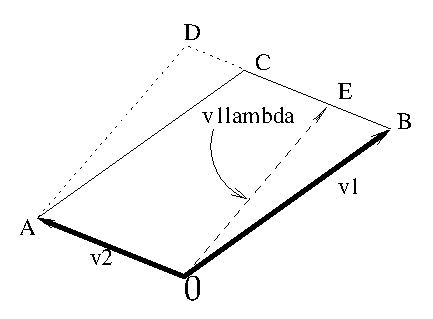
\includegraphics[width=3in]{v1v2-vol}
\par\end{centering}
\caption{The area of the parallelogram $0ACB$ spanned by $\mathbf{a}$ and
$\mathbf{b}$ is equal to the area of the parallelogram $0ADE$ spanned
by $\mathbf{a}$ and $\mathbf{b}+\alpha\mathbf{a}$ due to the equality
of areas $ACD$ and $0BE$.\label{fig:The-area-of1}}
\end{figure}


\subparagraph{Proof:}

The first property is a straightforward consequence of the sign rule
in the definition of $A$.

Proving the second property requires considering the cases $\lambda>0$
and $\lambda<0$ separately. If $\lambda>0$ then the orientation
of the pair $\left(\mathbf{a},\mathbf{b}\right)$ remains the same
and then it is clear that the property holds: When we rescale $\mathbf{a}$
by $\lambda$, the parallelogram is stretched and its area increases
by factor $\lambda$. If $\lambda<0$ then the orientation of the
parallelogram is reversed and the oriented area changes sign.

To prove the sum law, we consider  two cases: either $\mathbf{c}$
is parallel to $\mathbf{a}$ or it is not. If $\mathbf{c}$ is parallel
to $\mathbf{a}$, say $\mathbf{c}=\alpha\mathbf{a}$, we use Fig.~\ref{fig:The-area-of1}
to show that $A(\mathbf{a},\mathbf{b}+\lambda\mathbf{a})=A(\mathbf{a},\mathbf{b})$,
which yields the desired statement since $A(\mathbf{a},\lambda\mathbf{a})=0$.
If $\mathbf{c}$ is not parallel to $\mathbf{a}$, we use Fig.~\ref{fig:The-area-of2}
to show that $A(\mathbf{a},\mathbf{b}+\mathbf{c})=A(\mathbf{a},\mathbf{b})+A(\mathbf{a},\mathbf{c})$.
Analogous geometric constructions can be made for different possible
orientations of the vectors $\mathbf{a}$, $\mathbf{b}$, $\mathbf{c}$.\hfill{}$\blacksquare$

\begin{figure}
\begin{centering}
\psfrag{A}{$A$} \psfrag{B}{$B$} \psfrag{D}{$D$} \psfrag{C}{$C$} \psfrag{F}{$F$} \psfrag{E}{$E$}  \psfrag{a}{$\mathbf{a}$} \psfrag{b}{$\mathbf{b}$} \psfrag{c}{$\mathbf{c}$}\psfrag{b+c}{$\mathbf{b}+\mathbf{c}$}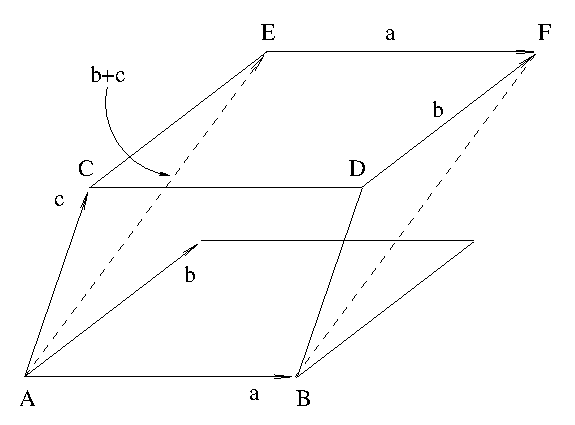
\includegraphics[width=3in]{2darea}
\par\end{centering}
\caption{The area of the parallelogram spanned by $\mathbf{a}$ and $\mathbf{b}$
(equal to the area of $CEFD$) plus the area of the parallelogram
spanned by $\mathbf{a}$ and $\mathbf{c}$ (the area of $ACDB$) equals
the area of the parallelogram spanned by $\mathbf{a}$ and $\mathbf{b}+\mathbf{c}$
(the area of $AEFB$) because of the equality of the areas of $ACE$
and $BDF$.\label{fig:The-area-of2}}
\end{figure}

It is relatively easy to compute the oriented area because of its
algebraic properties. Suppose the vectors $\mathbf{a}$ and $\mathbf{b}$
are given through their components in a standard basis $\left\{ \mathbf{e}_{1},\mathbf{e}_{2}\right\} $,
for instance 
\[
\mathbf{a}=\alpha_{1}\mathbf{e}_{1}+\alpha_{2}\mathbf{e}_{2},\quad\mathbf{b}=\beta_{1}\mathbf{e}_{1}+\beta_{2}\mathbf{e}_{2}.
\]
We assume, of course, that the vectors $\mathbf{e}_{1}$ and $\mathbf{e}_{2}$
are orthogonal to each other and have unit length, as is appropriate
in a Euclidean space. We also assume that the right angle is measured
from $\mathbf{e}_{1}$ to $\mathbf{e}_{2}$ in the counter-clockwise
direction, so that $A(\mathbf{e}_{1},\mathbf{e}_{2})=+1$. Then we
use the Statement and the properties $A(\mathbf{e}_{1},\mathbf{e}_{1})=0$,
$A(\mathbf{e}_{1},\mathbf{e}_{2})=1$, $A(\mathbf{e}_{2},\mathbf{e}_{2})=0$
to compute
\begin{align*}
A(\mathbf{a},\mathbf{b}) & =A(\alpha_{1}\mathbf{e}_{1}+\alpha_{2}\mathbf{e}_{2},\beta_{1}\mathbf{e}_{1}+\beta_{2}\mathbf{e}_{2})\\
 & =\alpha_{1}\beta_{2}A(\mathbf{e}_{1},\mathbf{e}_{2})+\alpha_{2}\beta_{1}A(\mathbf{e}_{2},\mathbf{e}_{1})\\
 & =\alpha_{1}\beta_{2}-\alpha_{2}\beta_{1}.
\end{align*}

The ordinary (unoriented) area is then obtained as the absolute value
of the oriented area, $Ar(\mathbf{a},\mathbf{b})=\left|A(\mathbf{a},\mathbf{b})\right|$.
It turns out that the oriented area, due to its strict linearity properties,
is a much more convenient and powerful construction than the unoriented
area.

\subsection{Parallelograms in $\mathbb{R}^{3}$ and in $\mathbb{R}^{n}$ \label{subsec:Area-of-two-dimensional-parallelograms}}

Let us now work in the Euclidean space $\mathbb{R}^{3}$ with a standard
basis $\left\{ \mathbf{e}_{1},\mathbf{e}_{2},\mathbf{e}_{3}\right\} $.
We can similarly try to characterize the area of a parallelogram spanned
by two vectors $\mathbf{a}$, $\mathbf{b}$. It is, however, not possible
to characterize the orientation of the area simply by a sign. We also
cannot use a geometric construction such as that in Fig.~\ref{fig:The-area-of2};
in fact it is \emph{not true} in three dimensions that the area spanned
by $\mathbf{a}$ and $\mathbf{b}+\mathbf{c}$ is equal to the sum
of $Ar(\mathbf{a},\mathbf{b})$ and $Ar(\mathbf{a},\mathbf{c})$.
Can we still define some kind of ``oriented area'' that obeys the
sum law?

Let us consider Fig.~\ref{fig:The-area-of2} as a figure showing
the \emph{projection} of the areas of the three parallelograms onto
some coordinate plane, say, the plane of the basis vectors $\left\{ \mathbf{e}_{1},\mathbf{e}_{2}\right\} $.
It is straightforward to see that the projections of the areas obey
the sum law as oriented areas.

\paragraph{Statement:}

Let $\mathbf{a},\mathbf{b}$ be two vectors in $\mathbb{R}^{3}$,
and let $P(\mathbf{a},\mathbf{b})$ be the parallelogram spanned by
these vectors. Denote by $P(\mathbf{a},\mathbf{b})_{\mathbf{e}_{1},\mathbf{e}_{2}}$
the parallelogram within the coordinate plane $\text{Span}\left\{ \mathbf{e}_{1},\mathbf{e}_{2}\right\} $
obtained by projecting $P(\mathbf{a},\mathbf{b})$ onto that coordinate
plane, and similarly for the other two coordinate planes. Denote by
$A(\mathbf{a},\mathbf{b})_{\mathbf{e}_{1},\mathbf{e}_{2}}$ the oriented
area of $P(\mathbf{a},\mathbf{b})_{\mathbf{e}_{1},\mathbf{e}_{2}}$.
Then $A(\mathbf{a},\mathbf{b})_{\mathbf{e}_{1},\mathbf{e}_{2}}$ is
a bilinear, antisymmetric function of $\mathbf{a}$ and $\mathbf{b}$.

\subparagraph{Proof:}

The projection onto the coordinate plane of $\mathbf{e}_{1},\mathbf{e}_{2}$
is a linear transformation. Hence, the vector $\mathbf{a}+\lambda\mathbf{b}$
is projected onto the sum of the projections of $\mathbf{a}$ and
$\lambda\mathbf{b}$. Then we apply the arguments in the proof of
Statement~\ref{subsec:Two-dimensional-oriented} to the \emph{projections}
of the vectors; in particular, Figs.~\ref{fig:The-area-of1} and~\ref{fig:The-area-of2}
are interpreted as showing the projections of all vectors onto the
coordinate plane $\mathbf{e}_{1},\mathbf{e}_{2}$. It is then straightforward
to see that all the properties of the oriented area hold for the projected
oriented areas. Details left as exercise.\hfill{}$\blacksquare$

It is therefore convenient to consider the oriented areas of the three
projections --- $A(\mathbf{a},\mathbf{b})_{\mathbf{e}_{1},\mathbf{e}_{2}}$,
$A(\mathbf{a},\mathbf{b})_{\mathbf{e}_{2},\mathbf{e}_{3}}$, $A(\mathbf{a},\mathbf{b})_{\mathbf{e}_{3},\mathbf{e}_{1}}$
--- as three components of a \emph{vector-valued} area $A(\mathbf{a},\mathbf{b})$
of the parallelogram spanned by $\mathbf{a},\mathbf{b}$. Indeed,
it can be shown that these three projected areas coincide with the
three Euclidean components of the vector product $\mathbf{a}\times\mathbf{b}$.
The vector product is the traditional way such areas are represented
in geometry: the vector $\mathbf{a}\times\mathbf{b}$ represents at
once the magnitude of the area and the orientation of the parallelogram.
One computes the unoriented area of a parallelogram as the length
of the vector $\mathbf{a}\times\mathbf{b}$ representing the oriented
area,
\[
Ar(\mathbf{a},\mathbf{b})=\left[A(\mathbf{a},\mathbf{b})_{\mathbf{e}_{1},\mathbf{e}_{2}}^{2}+A(\mathbf{a},\mathbf{b})_{\mathbf{e}_{2},\mathbf{e}_{3}}^{2}+A(\mathbf{a},\mathbf{b})_{\mathbf{e}_{3},\mathbf{e}_{1}}^{2}\right]^{\frac{1}{2}}.
\]

However, the vector product cannot be generalized to all higher-dimen\-sion\-al
spaces. Luckily, the vector product does not play an essential role
in the construction of the oriented area. 

Instead of working with the vector product, we will generalize the
idea of projecting the parallelogram onto coordinate planes. Consider
a parallelogram spanned by vectors $\mathbf{a},\mathbf{b}$ in an
$n$-dimen\-sion\-al Euclidean space $V$ with the standard basis
$\left\{ \mathbf{e}_{1},...,\mathbf{e}_{n}\right\} $. While in three-dimen\-sion\-al
space we had just three projections (onto the coordinate planes $xy$,
$xz$, $yz$), in an $n$-dimen\-sion\-al space we have $\frac{1}{2}n(n-1)$
coordinate planes, which can be denoted by $\text{Span}\left\{ \mathbf{e}_{i},\mathbf{e}_{j}\right\} $
(with $1\leq i<j\leq n$). We may construct the $\frac{1}{2}n(n-1)$
projections of the parallelogram onto these coordinate planes. Each
of these projections has an oriented area; that area is a bilinear,
antisymmetric number-valued function of the vectors $\mathbf{a},\mathbf{b}$.
(The proof of the Statement above does not use the fact that the space
is \emph{three}-dimen\-sion\-al!) We may then regard these $\frac{1}{2}n(n-1)$
numbers as the components of a vector representing the oriented area
of the parallelogram. It is clear that all these components are needed
in order to describe the actual geometric \emph{orientation} of the
parallelogram in the $n$-dimen\-sion\-al space.

We arrived at the idea that the oriented area of the parallelogram
spanned by $\mathbf{a},\mathbf{b}$ is an antisymmetric, bilinear
function $A(\mathbf{a},\mathbf{b})$ whose value is a vector with
$\frac{1}{2}n(n-1)$ components, i.e.~a vector \emph{in a new space}
--- the ``space of oriented areas,'' as it were. This space is
$\frac{1}{2}n(n-1)$-dimen\-sion\-al. We will construct this space
explicitly below; it is the space of bivectors, to be denoted by $\wedge^{2}V$. 

We will see that the unoriented area of the parallelogram is computed
as the \emph{length} of the vector $A(\mathbf{a},\mathbf{b})$, i.e.~as
the square root of the sum of squares of the areas of the projections
of the parallelogram onto the coordinate planes. This is a generalization
of the Pythagoras theorem to areas in higher-dimen\-sion\-al spaces.

The analogy between ordinary vectors and vector-val\-ued areas can
be understood visually as follows. A straight line segment in an $n$-dimen\-sion\-al
space is represented by a vector whose $n$ components (in an orthonormal
basis) are the signed lengths of the $n$ projections of the line
segment onto the coordinate axes. (The components are \emph{signed},
or \emph{oriented}, i.e.~taken with a negative sign if the orientation
of the vector is opposite to the orientation of the axis.) The length
of a straight line segment, i.e.~the length of the vector $\mathbf{v}$,
is then computed as $\sqrt{\left\langle \mathbf{v},\mathbf{v}\right\rangle }$.
The scalar product $\left\langle \mathbf{v},\mathbf{v}\right\rangle $
is equal to the sum of squared lengths of the projections because
we are using an orthonormal basis. A parallelogram in space is represented
by a vector $\psi$ whose ${n \choose 2}$ components are the \emph{oriented}
areas of the ${n \choose 2}$ projections of the parallelogram onto
the coordinate planes. (The vector $\psi$ belongs to the space of
oriented areas, not to the original $n$-dimen\-sion\-al space.)
The numerical value of the area of the parallelogram is then computed
as $\sqrt{\left\langle \psi,\psi\right\rangle }$. The scalar product
$\left\langle \psi,\psi\right\rangle $ in the space of oriented areas
is equal to the sum of squared areas of the projections because the
${n \choose 2}$ unit areas in the coordinate planes are an orthonormal
basis (according to the definition of the scalar product in the space
of oriented areas).

The generalization of the Pythagoras theorem holds not only for areas
but also for higher-dimen\-sion\-al volumes. A general proof of
this theorem will be given in Sec.~\ref{proof-of-pythagoras}, using
the exterior product and several other constructions to be developed
below.

\section{Exterior product\label{subsec:Definition-of-the-exterior}}

In the previous section I motivated the introduction of the antisymmetric
product by showing its connection to areas and volumes. In this section
I will give the definition and work out the properties of the exterior
product in a purely algebraic manner, without using any geometric
intuition. This will enable us to work with vectors in arbitrary dimensions,
to obtain many useful results, and eventually also to appreciate more
fully the geometric significance of the exterior product. 

As explained in Sec.~\ref{subsec:Area-of-two-dimensional-parallelograms},
it is possible to represent the oriented area of a parallelogram by
a vector in some auxiliary space. The oriented area is much more convenient
to work with because it is a \emph{bilinear} function of the vectors
$\mathbf{a}$ and $\mathbf{b}$ (this is explained in detail in Sec.~\ref{subsec:Motivation-for-exterior}).
``Product'' is another word for ``bilinear function.'' We have
also seen that the oriented area is an \emph{antisymmetric} function
of the vectors $\mathbf{a}$ and $\mathbf{b}$.

In three dimensions, an oriented area is represented by the cross
product $\mathbf{a}\times\mathbf{b}$, which is indeed an antisymmetric
and bilinear product. So we expect that the oriented area in higher
dimensions can be represented by some kind of new antisymmetric product
of $\mathbf{a}$ and $\mathbf{b}$; let us denote this product (to
be defined below) by $\mathbf{a}\wedge\mathbf{b}$, pronounced ``a
wedge b.'' The value of $\mathbf{a}\wedge\mathbf{b}$ will be a vector
in a \emph{new} vector space. We will also construct this new space
explicitly.

\subsection{Definition of exterior product}

Like the tensor product space, the space of exterior products can
be defined solely by its algebraic properties. We can consider the
space of \emph{formal} \emph{expressions} like $\mathbf{a}\wedge\mathbf{b}$,
$3\mathbf{a}\wedge\mathbf{b}+2\mathbf{c}\wedge\mathbf{d}$, etc.,
and \emph{require} the properties of an antisymmetric, bilinear product
to hold.

Here is a more formal definition of the exterior product space: We
will construct an antisymmetric product ``by hand,'' using the tensor
product space.

\paragraph{Definition 1:}

Given a vector space $V$, we define a new vector space $V\wedge V$
called the \textbf{exterior product}\index{exterior product} (or
antisymmetric tensor product, or alternating product, or \textbf{wedge
product}\index{wedge product}) of two copies of $V$. The space $V\wedge V$
is the subspace in $V\otimes V$ consisting of all \textbf{antisymmetric}
tensors, i.e.~tensors of the form
\[
\mathbf{v}_{1}\otimes\mathbf{v}_{2}-\mathbf{v}_{2}\otimes\mathbf{v}_{1},\quad\mathbf{v}_{1,2}\in V,
\]
and all linear combinations of such tensors. The exterior product
of two vectors $\mathbf{v}_{1}$ and $\mathbf{v}_{2}$ is the expression
shown above; it is obviously an antisymmetric and bilinear function
of $\mathbf{v}_{1}$ and $\mathbf{v}_{2}$.

For example, here is one particular element from $V\wedge V$, which
we write in two different ways using the axioms of the tensor product:
\begin{align}
\left(\mathbf{u}+\mathbf{v}\right)\otimes\left(\mathbf{v}+\mathbf{w}\right)-\left(\mathbf{v}+\mathbf{w}\right)\otimes\left(\mathbf{u}+\mathbf{v}\right)=\mathbf{u}\otimes\mathbf{v}-\mathbf{v}\otimes\mathbf{u}\nonumber \\
+\mathbf{u}\otimes\mathbf{w}-\mathbf{w}\otimes\mathbf{u}+\mathbf{v}\otimes\mathbf{w}-\mathbf{w}\otimes\mathbf{v}\in V\wedge V.\label{eq:uvw calc 1}
\end{align}


\subparagraph{Remark:}

A tensor $\mathbf{v}_{1}\otimes\mathbf{v}_{2}\in V\otimes V$ is not
equal to the tensor $\mathbf{v}_{2}\otimes\mathbf{v}_{1}$ if $\mathbf{v}_{1}\neq\mathbf{v}_{2}$.
This is so because there is no identity among the axioms of the tensor
product that would allow us to exchange the factors $\mathbf{v}_{1}$
and $\mathbf{v}_{2}$ in the expression $\mathbf{v}_{1}\otimes\mathbf{v}_{2}$.

\paragraph{Exercise 1:}

Prove that the ``exchange map'' $\hat{T}\left(\mathbf{v}_{1}\otimes\mathbf{v}_{2}\right)\equiv\mathbf{v}_{2}\otimes\mathbf{v}_{1}$
is a canonically defined, linear map of $V\otimes V$ into itself.
Show that $\hat{T}$ has only two eigenvalues which are $\pm1$. Give
examples of eigenvectors with eigenvalues $+1$ and $-1$. Show that
the subspace $V\wedge V\subset V\otimes V$ is the eigenspace of the
exchange operator $\hat{T}$ with eigenvalue $-1$

\emph{Hint:} $\hat{T}\hat{T}=\hat{1}_{V\otimes V}$. Consider tensors
of the form $\mathbf{u}\otimes\mathbf{v}\pm\mathbf{v}\otimes\mathbf{u}$
as candidate eigenvectors of $\hat{T}$.\hfill{}$\blacksquare$

It is quite cumbersome to perform calculations in the tensor product
notation as we did in Eq.~(\ref{eq:uvw calc 1}). So let us write
the exterior product as $\mathbf{u}\wedge\mathbf{v}$ instead of $\mathbf{u}\otimes\mathbf{v}-\mathbf{v}\otimes\mathbf{u}$.
It is then straightforward to see that the ``wedge'' symbol $\wedge$
indeed works like an anti-commutative multiplication, as we intended.
The rules of computation are summarized in the following statement.

\paragraph{Statement 1:}

One may save time and write $\mathbf{u}\otimes\mathbf{v}-\mathbf{v}\otimes\mathbf{u}\equiv\mathbf{u}\wedge\mathbf{v}\in V\wedge V$,
and the result of any calculation will be correct, as long as one
follows the rules:
\begin{align}
\mathbf{u}\wedge\mathbf{v} & =-\mathbf{v}\wedge\mathbf{u},\label{eq:uv antisymm}\\
\left(\lambda\mathbf{u}\right)\wedge\mathbf{v} & =\lambda\left(\mathbf{u}\wedge\mathbf{v}\right),\\
\left(\mathbf{u}+\mathbf{v}\right)\wedge\mathbf{x} & =\mathbf{u}\wedge\mathbf{x}+\mathbf{v}\wedge\mathbf{x}.\label{eq:uv distrib}
\end{align}
It follows also that $\mathbf{u}\wedge\left(\lambda\mathbf{v}\right)=\lambda\left(\mathbf{u}\wedge\mathbf{v}\right)$
and that $\mathbf{v}\wedge\mathbf{v}=0$. (These identities hold for
any vectors $\mathbf{u},\mathbf{v}\in V$ and any scalars $\lambda\in\mathbb{K}$.)

\subparagraph{Proof:}

These properties are direct consequences of the axioms of the tensor
product when applied to antisymmetric tensors. For example, the calculation~(\ref{eq:uvw calc 1})
now requires a simple expansion of brackets,
\[
\left(\mathbf{u}+\mathbf{v}\right)\wedge\left(\mathbf{v}+\mathbf{w}\right)=\mathbf{u}\wedge\mathbf{v}+\mathbf{u}\wedge\mathbf{w}+\mathbf{v}\wedge\mathbf{w}.
\]
Here we removed the term $\mathbf{v}\wedge\mathbf{v}$ which vanishes
due to the antisymmetry of $\wedge$. Details left as exercise.\hfill{}$\blacksquare$

Elements of the space $V\wedge V$, such as $\mathbf{a}\wedge\mathbf{b}+\mathbf{c}\wedge\mathbf{d}$,
are sometimes called \textbf{bivectors}\index{bivector}.\footnote{It is important to note that a bivector is not necessarily expressible
as a single-term product of two vectors; see the Exercise at the end
of Sec.~\ref{subsec:Properties-of-the-ext-powers}.\index{single-term exterior products}} We will also want to define the exterior product of more than two
vectors. To define the exterior product of \emph{three} vectors, we
consider the subspace of $V\otimes V\otimes V$ that consists of antisymmetric
tensors of the form
\begin{align}
\mathbf{a}\otimes\mathbf{b}\otimes\mathbf{c}-\mathbf{b}\otimes\mathbf{a}\otimes\mathbf{c}+\mathbf{c}\otimes\mathbf{a}\otimes\mathbf{b}-\mathbf{c}\otimes\mathbf{b}\otimes\mathbf{a}\nonumber \\
+\mathbf{b}\otimes\mathbf{c}\otimes\mathbf{a}-\mathbf{a}\otimes\mathbf{c}\otimes\mathbf{b}\label{eq:antisym 3}
\end{align}
and linear combinations of such tensors. These tensors are called
\textbf{totally antisymmetric\index{totally antisymmetric}} because
they can be viewed as (tensor-valued) functions of the vectors $\mathbf{a},\mathbf{b},\mathbf{c}$
that change sign under exchange of any two vectors. The expression
in Eq.~(\ref{eq:antisym 3}) will be denoted for brevity by $\mathbf{a}\wedge\mathbf{b}\wedge\mathbf{c}$,
similarly to the exterior product of two vectors, $\mathbf{a}\otimes\mathbf{b}-\mathbf{b}\otimes\mathbf{a}$,
which is denoted for brevity by $\mathbf{a}\wedge\mathbf{b}$. Here
is a general definition.

\paragraph{Definition 2:}

The \textbf{exterior product\index{exterior product} of $k$ copies}
of $V$ (also called the \textbf{$k$-th exterior power} of $V$)
is denoted by $\wedge^{k}V$ and is defined as the subspace of totally
antisymmetric tensors within $V\otimes...\otimes V$. In the concise
notation, this is the space spanned by expressions of the form
\[
\mathbf{v}_{1}\wedge\mathbf{v}_{2}\wedge...\wedge\mathbf{v}_{k},\quad\mathbf{v}_{j}\in V,
\]
assuming that the properties of the wedge product (linearity and antisymmetry)
hold as given by Statement~1. For instance, 
\begin{equation}
\mathbf{u}\wedge\mathbf{v}_{1}\wedge...\wedge\mathbf{v}_{k}=\left(-1\right)^{k}\mathbf{v}_{1}\wedge...\wedge\mathbf{v}_{k}\wedge\mathbf{u}\label{eq:uv pull}
\end{equation}
(``pulling a vector through $k$ other vectors changes sign $k$
times'').\hfill{}$\blacksquare$

The previously defined space of bivectors is in this notation $V\wedge V\equiv\wedge^{2}V$.
A natural extension of this notation is $\wedge^{0}V=\mathbb{K}$
and $\wedge^{1}V=V$. I will also use the following ``wedge product''
notation,
\[
\bigwedge_{k=1}^{n}\mathbf{v}_{k}\equiv\mathbf{v}_{1}\wedge\mathbf{v}_{2}\wedge...\wedge\mathbf{v}_{n}.
\]

Tensors from the space $\wedge^{n}V$ are also called $n$-\textbf{vectors}\index{$n$-vectors}
or \textbf{antisymmetric tensors}\index{antisymmetric tensor} of
rank $n$.

\paragraph{Question:}

How to compute expressions containing multiple products such as $\mathbf{a}\wedge\mathbf{b}\wedge\mathbf{c}$?

\subparagraph{Answer:}

Apply the rules shown in Statement~1. For example, one can permute
adjacent vectors and change sign,
\[
\mathbf{a}\wedge\mathbf{b}\wedge\mathbf{c}=-\mathbf{b}\wedge\mathbf{a}\wedge\mathbf{c}=\mathbf{b}\wedge\mathbf{c}\wedge\mathbf{a},
\]
one can expand brackets,
\[
\mathbf{a}\wedge(\mathbf{x}+4\mathbf{y})\wedge\mathbf{b}=\mathbf{a}\wedge\mathbf{x}\wedge\mathbf{b}+4\mathbf{a}\wedge\mathbf{y}\wedge\mathbf{b},
\]
and so on. If the vectors $\mathbf{a},\mathbf{b},\mathbf{c}$ are
given as linear combinations of some basis vectors $\left\{ \mathbf{e}_{j}\right\} $,
we can thus reduce $\mathbf{a}\wedge\mathbf{b}\wedge\mathbf{c}$ to
a linear combination of exterior products of basis vectors, such as
$\mathbf{e}_{1}\wedge\mathbf{e}_{2}\wedge\mathbf{e}_{3}$, $\mathbf{e}_{1}\wedge\mathbf{e}_{2}\wedge\mathbf{e}_{4}$,
etc.

\paragraph{Question:}

The notation $\mathbf{a}\wedge\mathbf{b}\wedge\mathbf{c}$ suggests
that the exterior product is associative,
\[
\mathbf{a}\wedge\mathbf{b}\wedge\mathbf{c}=\left(\mathbf{a}\wedge\mathbf{b}\right)\wedge\mathbf{c}=\mathbf{a}\wedge(\mathbf{b}\wedge\mathbf{c}).
\]
How can we make sense of this?

\subparagraph{Answer:}

If we want to be pedantic, we need to define the exterior product
operation $\wedge$ between a single-term bivector $\mathbf{a}\wedge\mathbf{b}$
and a vector $\mathbf{c}$, such that the result is \emph{by} \emph{definition}
the 3-vector $\mathbf{a}\wedge\mathbf{b}\wedge\mathbf{c}$. We then
define the same operation on linear combinations of single-term bivectors,
\[
\left(\mathbf{a}\wedge\mathbf{b}+\mathbf{x}\wedge\mathbf{y}\right)\wedge\mathbf{c}\equiv\mathbf{a}\wedge\mathbf{b}\wedge\mathbf{c}+\mathbf{x}\wedge\mathbf{y}\wedge\mathbf{c}.
\]
Thus we have defined the exterior product between $\wedge^{2}V$ and
$V$, the result being a 3-vector from $\wedge^{3}V$. We then need
to verify that the results do not depend on the choice of the vectors
such as $\mathbf{a},\mathbf{b},\mathbf{x},\mathbf{y}$ in the representation
of a bivector: A different representation can be achieved only by
using the properties of the exterior product (i.e.~the axioms of
the tensor product), e.g.~we may replace $\mathbf{a}\wedge\mathbf{b}$
by $-\mathbf{b}\wedge\left(\mathbf{a}+\lambda\mathbf{b}\right)$.
It is easy to verify that any such replacements will not modify the
resulting 3-vector, e.g. 
\[
\mathbf{a}\wedge\mathbf{b}\wedge\mathbf{c}=-\mathbf{b}\wedge\left(\mathbf{a}+\lambda\mathbf{b}\right)\wedge\mathbf{c},
\]
again due to the properties of the exterior product. This consideration
shows that calculations with exterior products are consistent with
our algebraic intuition. We may indeed compute $\mathbf{a}\wedge\mathbf{b}\wedge\mathbf{c}$
as $\left(\mathbf{a}\wedge\mathbf{b}\right)\wedge\mathbf{c}$ or as
$\mathbf{a}\wedge\left(\mathbf{b}\wedge\mathbf{c}\right)$.

\paragraph{Example~1:}

Suppose we work in $\mathbb{R}^{3}$ and have vectors $\mathbf{a}=\left(0,\frac{1}{2},-\frac{1}{2}\right)$,
$\mathbf{b}=\left(2,-2,0\right)$, $\mathbf{c}=\left(-2,5,-3\right)$.
Let us compute various exterior products. Calculations are easier
if we introduce the basis $\left\{ \mathbf{e}_{1},\mathbf{e}_{2},\mathbf{e}_{3}\right\} $
explicitly:
\[
\mathbf{a}=\frac{1}{2}\left(\mathbf{e}_{2}-\mathbf{e}_{3}\right),\quad\mathbf{b}=2(\mathbf{e}_{1}-\mathbf{e}_{2}),\quad\mathbf{c}=-2\mathbf{e}_{1}+5\mathbf{e}_{2}-3\mathbf{e}_{3}.
\]
We compute the 2-vector $\mathbf{a}\wedge\mathbf{b}$ by using the
properties of the exterior product, such as $\mathbf{x}\wedge\mathbf{x}=0$
and $\mathbf{x}\wedge\mathbf{y}=-\mathbf{y}\wedge\mathbf{x}$, and
simply expanding the brackets as usual in algebra:
\begin{align*}
\mathbf{a}\wedge\mathbf{b} & =\frac{1}{2}\left(\mathbf{e}_{2}-\mathbf{e}_{3}\right)\wedge2\left(\mathbf{e}_{1}-\mathbf{e}_{2}\right)\\
 & =\left(\mathbf{e}_{2}-\mathbf{e}_{3}\right)\wedge\left(\mathbf{e}_{1}-\mathbf{e}_{2}\right)\\
 & =\mathbf{e}_{2}\wedge\mathbf{e}_{1}-\mathbf{e}_{3}\wedge\mathbf{e}_{1}-\mathbf{e}_{2}\wedge\mathbf{e}_{2}+\mathbf{e}_{3}\wedge\mathbf{e}_{2}\\
 & =-\mathbf{e}_{1}\wedge\mathbf{e}_{2}+\mathbf{e}_{1}\wedge\mathbf{e}_{3}-\mathbf{e}_{2}\wedge\mathbf{e}_{3}.
\end{align*}
The last expression is the result; note that now there is nothing
more to compute or to simplify. The expressions such as $\mathbf{e}_{1}\wedge\mathbf{e}_{2}$
are the basic expressions out of which the space $\mathbb{R}^{3}\wedge\mathbb{R}^{3}$
is built. Below (Sec.~\ref{subsec:Properties-of-the-ext-powers})
we will show formally that the set of these expressions is a basis
in the space $\mathbb{R}^{3}\wedge\mathbb{R}^{3}$.

Let us also compute the 3-vector $\mathbf{a}\wedge\mathbf{b}\wedge\mathbf{c}$,
\begin{align*}
 & \mathbf{a}\wedge\mathbf{b}\wedge\mathbf{c}=\left(\mathbf{a}\wedge\mathbf{b}\right)\wedge\mathbf{c}\\
 & =\left(-\mathbf{e}_{1}\wedge\mathbf{e}_{2}+\mathbf{e}_{1}\wedge\mathbf{e}_{3}-\mathbf{e}_{2}\wedge\mathbf{e}_{3}\right)\wedge(-2\mathbf{e}_{1}+5\mathbf{e}_{2}-3\mathbf{e}_{3}).
\end{align*}
When we expand the brackets here, terms such as $\mathbf{e}_{1}\wedge\mathbf{e}_{2}\wedge\mathbf{e}_{1}$
will vanish because 
\[
\mathbf{e}_{1}\wedge\mathbf{e}_{2}\wedge\mathbf{e}_{1}=-\mathbf{e}_{2}\wedge\mathbf{e}_{1}\wedge\mathbf{e}_{1}=0,
\]
so only terms containing all different vectors need to be kept, and
we find
\begin{align*}
\mathbf{a}\wedge\mathbf{b}\wedge\mathbf{c} & =3\mathbf{e}_{1}\wedge\mathbf{e}_{2}\wedge\mathbf{e}_{3}+5\mathbf{e}_{1}\wedge\mathbf{e}_{3}\wedge\mathbf{e}_{2}+2\mathbf{e}_{2}\wedge\mathbf{e}_{3}\wedge\mathbf{e}_{1}\\
 & =\left(3-5+2\right)\mathbf{e}_{1}\wedge\mathbf{e}_{2}\wedge\mathbf{e}_{3}=0.
\end{align*}
We note that all the terms are proportional to the 3-vector $\mathbf{e}_{1}\wedge\mathbf{e}_{2}\wedge\mathbf{e}_{3}$,
so only the coefficient in front of $\mathbf{e}_{1}\wedge\mathbf{e}_{2}\wedge\mathbf{e}_{3}$
was needed; then, by coincidence, that coefficient turned out to be
zero. So the result is the zero 3-vector.\hfill{}$\blacksquare$

\paragraph{Question:}

Our original goal was to introduce a bilinear, antisymmetric product
of vectors in order to obtain a geometric representation of oriented
areas. Instead, $\mathbf{a}\wedge\mathbf{b}$ was defined algebraically,
through tensor products. It is clear that $\mathbf{a}\wedge\mathbf{b}$
is antisymmetric and bilinear, but why does it represent an oriented
area?

\subparagraph{Answer:}

Indeed, it may not be immediately clear why oriented areas should
be elements of $V\wedge V$. We have seen that the oriented area $A(\mathbf{x},\mathbf{y})$
is an antisymmetric and bilinear function of the two vectors $\mathbf{x}$
and $\mathbf{y}$. Right now we have constructed the space $V\wedge V$
simply as the \emph{space of antisymmetric products}. By constructing
that space merely out of the axioms of the antisymmetric product,
we already covered \emph{every} \emph{possible} bilinear antisymmetric
product. This means that \emph{any} antisymmetric and bilinear function
of the two vectors $\mathbf{x}$ and $\mathbf{y}$ is proportional
to $\mathbf{x}\wedge\mathbf{y}$ or, more generally, is a \emph{linear}
\emph{function} of $\mathbf{x}\wedge\mathbf{y}$ (perhaps with values
in a different space). Therefore, the space of oriented areas (that
is, the space of linear combinations of $A(\mathbf{x},\mathbf{y})$
for various $\mathbf{x}$ and $\mathbf{y}$) is in any case mapped
to a subspace of $V\wedge V$. We have also seen that oriented areas
in $N$ dimensions can be represented through ${N \choose 2}$ projections,
which indicates that they are vectors in some ${N \choose 2}$-dimen\-sion\-al
space. We will see below that the space $V\wedge V$ has exactly this
dimension (Theorem~2 in Sec.~\ref{subsec:Properties-of-the-ext-powers}).
Therefore, we can expect that the space of oriented areas coincides
with $V\wedge V$. Below we will be working in a space $V$ with a
scalar product, where the notions of area and volume are well defined.
Then we will see (Sec.~\ref{subsec:Volumes-of-k-dimensional}) that
tensors from $V\wedge V$ and the higher exterior powers of $V$ indeed
correspond in a natural way to oriented areas, or more generally to
oriented volumes of a certain dimension.

\paragraph{Remark: Origin of the name ``exterior.''}

The construction of the exterior product\index{exterior product!origin of the name}
is a modern formulation of the ideas dating back to H. Grassmann (1844).
A 2-vector $\mathbf{a}\wedge\mathbf{b}$ is interpreted geometrically
as the oriented area of the parallelogram spanned by the vectors $\mathbf{a}$
and $\mathbf{b}$. Similarly, a 3-vector $\mathbf{a}\wedge\mathbf{b}\wedge\mathbf{c}$
represents the oriented 3-volume of a parallelepiped spanned by $\left\{ \mathbf{a},\mathbf{b},\mathbf{c}\right\} $.
Due to the antisymmetry of the exterior product, we have $(\mathbf{a}\wedge\mathbf{b})\wedge(\mathbf{a}\wedge\mathbf{c})=0$,
$(\mathbf{a}\wedge\mathbf{b}\wedge\mathbf{c})\wedge(\mathbf{b}\wedge\mathbf{d})=0$,
etc. We can interpret this geometrically by saying that the ``product''
of two volumes is zero if these volumes have a vector in common. This
motivated Grassmann to call his antisymmetric product ``exterior.''
In his reasoning, the product of two ``extensive quantities'' (such
as lines, areas, or volumes) is nonzero only when each of the two
quantities is geometrically ``to the exterior'' (outside) of the
other.

\paragraph{Exercise 2:}

Show that in a \emph{two}-dimensional space $V$, any 3-vector such
as $\mathbf{a}\wedge\mathbf{b}\wedge\mathbf{c}$ can be simplified
to the zero 3-vector. Prove the same for $n$-vectors in $N$-dimensional
spaces when $n>N$.\hfill{}$\blacksquare$

One can also consider the exterior powers of the \emph{dual} space
$V^{*}$. Tensors from $\wedge^{n}V^{*}$ are usually (for historical
reasons) called $n$-\textbf{forms}\index{$n$-forms} (rather than
``$n$-covectors'').

\paragraph{Question:}

Where is the star here, really? Is the space $\wedge^{n}\left(V^{*}\right)$
different from $\left(\wedge^{n}V\right)^{*}$?

\subparagraph{Answer:}

Good that you asked. These spaces are canonically isomorphic, but
there is a subtle technical issue worth mentioning. Consider an example:
$\mathbf{a}^{*}\wedge\mathbf{b}^{*}\in\wedge^{2}(V^{*})$ can act
upon $\mathbf{u}\wedge\mathbf{v}\in\wedge^{2}V$ by the standard tensor
product rule, namely $\mathbf{a}^{*}\otimes\mathbf{b}^{*}$ acts on
$\mathbf{u}\otimes\mathbf{v}$ as 
\[
\left(\mathbf{a}^{*}\otimes\mathbf{b}^{*}\right)\left(\mathbf{u}\otimes\mathbf{v}\right)=\mathbf{a}^{*}(\mathbf{u})\,\mathbf{b}^{*}(\mathbf{v}),
\]
so by using the definition of $\mathbf{a}^{*}\wedge\mathbf{b}^{*}$
and $\mathbf{u}\wedge\mathbf{v}$ through the tensor product, we find
\begin{align*}
\left(\mathbf{a}^{*}\wedge\mathbf{b}^{*}\right)\left(\mathbf{u}\wedge\mathbf{v}\right) & =\left(\mathbf{a}^{*}\otimes\mathbf{b}^{*}-\mathbf{b}^{*}\otimes\mathbf{a}^{*}\right)\left(\mathbf{u}\otimes\mathbf{v}-\mathbf{v}\otimes\mathbf{u}\right)\\
 & =2\mathbf{a}^{*}(\mathbf{u})\,\mathbf{b}^{*}(\mathbf{v})-2\mathbf{b}^{*}(\mathbf{u})\,\mathbf{a}^{*}(\mathbf{v}).
\end{align*}
We got a \textbf{combinatorial} \textbf{factor}\index{combinatorial factor}
2, that is, a factor that arises because we have \emph{two} permutations
of the set $\left(\mathbf{a},\mathbf{b}\right)$. With $\wedge^{n}\left(V^{*}\right)$
and $\left(\wedge^{n}V\right)^{*}$ we get a factor $n!$. It is not
always convenient to have this combinatorial factor. For example,
in a finite number field the number $n!$ might be \emph{equal to
zero} for large enough $n$. In these cases we could \emph{redefine}
the action of $\mathbf{a}^{*}\wedge\mathbf{b}^{*}$ on $\mathbf{u}\wedge\mathbf{v}$
as 
\[
\left(\mathbf{a}^{*}\wedge\mathbf{b}^{*}\right)\left(\mathbf{u}\wedge\mathbf{v}\right)\equiv\mathbf{a}^{*}(\mathbf{u})\,\mathbf{b}^{*}(\mathbf{v})-\mathbf{b}^{*}(\mathbf{u})\,\mathbf{a}^{*}(\mathbf{v}).
\]
 If we are not working in a finite number field, we are able to divide
by any integer, so we may keep combinatorial factors in the denominators
of expressions where such factors appear. For example, if $\left\{ \mathbf{e}_{j}\right\} $
is a basis in $V$ and $\omega=\mathbf{e}_{1}\wedge...\wedge\mathbf{e}_{N}$
is the corresponding basis tensor in the one-dimen\-sion\-al space
$\wedge^{N}V$, the dual basis tensor in $\left(\wedge^{N}V\right)^{*}$
could be defined by 
\[
\omega^{*}=\frac{1}{N!}\mathbf{e}_{1}^{*}\wedge...\wedge\mathbf{e}_{N}^{*},\quad\text{so that}\:\omega^{*}(\omega)=1.
\]
The need for such combinatorial factors is a minor technical inconvenience
that does not arise too often. We may give the following definition
that avoids dividing by combinatorial factors (but now we use permutations;
see Appendix~\ref{subsec:Properties-of-permutations}).

\paragraph{Definition 3:}

The action of a $k$-form $\mathbf{f}_{1}^{*}\wedge...\wedge\mathbf{f}_{k}^{*}$
on a $k$-vector $\mathbf{v}_{1}\wedge...\wedge\mathbf{v}_{k}$ is
defined by
\[
\sum_{\sigma}(-1)^{\left|\sigma\right|}\mathbf{f}_{1}^{*}(\mathbf{v}_{\sigma(1)})...\mathbf{f}_{k}^{*}(\mathbf{v}_{\sigma(k)}),
\]
where the summation is performed over all permutations $\sigma$ of
the ordered set $\left(1,...,k\right)$.

\paragraph{Example~2:}

With $k=3$ we have
\begin{align*}
 & (\mathbf{p}^{*}\wedge\mathbf{q}^{*}\wedge\mathbf{r}^{*})(\mathbf{a}\wedge\mathbf{b}\wedge\mathbf{c})\\
 & =\mathbf{p}^{*}(\mathbf{a})\mathbf{q}^{*}(\mathbf{b})\mathbf{r}^{*}(\mathbf{c})-\mathbf{p}^{*}(\mathbf{b})\mathbf{q}^{*}(\mathbf{a})\mathbf{r}^{*}(\mathbf{c})\\
 & +\mathbf{p}^{*}(\mathbf{b})\mathbf{q}^{*}(\mathbf{c})\mathbf{r}^{*}(\mathbf{a})-\mathbf{p}^{*}(\mathbf{c})\mathbf{q}^{*}(\mathbf{b})\mathbf{r}^{*}(\mathbf{a})\\
 & +\mathbf{p}^{*}(\mathbf{c})\mathbf{q}^{*}(\mathbf{a})\mathbf{r}^{*}(\mathbf{b})-\mathbf{p}^{*}(\mathbf{c})\mathbf{q}^{*}(\mathbf{b})\mathbf{r}^{*}(\mathbf{a}).
\end{align*}


\paragraph{Exercise 3:}

a) Show that $\mathbf{a}\wedge\mathbf{b}\wedge\omega=\omega\wedge\mathbf{a}\wedge\mathbf{b}$
where $\omega$ is any antisymmetric tensor (e.g.~$\omega=\mathbf{x}\wedge\mathbf{y}\wedge\mathbf{z}$).

b) Show that
\[
\omega_{1}\wedge\mathbf{a}\wedge\omega_{2}\wedge\mathbf{b}\wedge\omega_{3}=-\omega_{1}\wedge\mathbf{b}\wedge\omega_{2}\wedge\mathbf{a}\wedge\omega_{3},
\]
where $\omega_{1}$, $\omega_{2}$, $\omega_{3}$ are arbitrary antisymmetric
tensors and $\mathbf{a},\mathbf{b}$ are vectors. 

c) Due to antisymmetry,  $\mathbf{a}\wedge\mathbf{a}=0$ for any vector
$\mathbf{a}\in V$. Is it also true that $\omega\wedge\omega=0$ for
any bivector $\omega\in\wedge^{2}V$?

\subsection{{*} Symmetric tensor product}

\paragraph{Question:}

At this point it is still unclear why the antisymmetric definition
is at all useful. Perhaps we could define something else, say the
symmetric product, instead of the exterior product? We could try to
define a product, say $\mathbf{a}\odot\mathbf{b}$, with some other
property, such as
\[
\mathbf{a}\odot\mathbf{b}=2\mathbf{b}\odot\mathbf{a}.
\]


\subparagraph{Answer:}

This does not work because, for example, we would have
\[
\mathbf{b}\odot\mathbf{a}=2\mathbf{a}\odot\mathbf{b}=4\mathbf{b}\odot\mathbf{a},
\]
so all the ``$\odot$'' products would have to vanish.

We can define the \emph{symmetric} tensor product, $\otimes_{S}$,
with the property
\[
\mathbf{a}\otimes_{S}\mathbf{b}=\mathbf{b}\otimes_{S}\mathbf{a},
\]
but it is impossible to define anything else in a similar fashion.\footnote{This is a theorem due to Grassmann (1862).} 

The antisymmetric tensor product is the eigenspace (within $V\otimes V$)
of the exchange operator $\hat{T}$ with eigenvalue $-1$. That operator
has only eigenvectors with eigenvalues $\pm1$, so the only other
possibility is to consider the eigenspace with eigenvalue $+1$. This
eigenspace is spanned by symmetric tensors of the form $\mathbf{u}\otimes\mathbf{v}+\mathbf{v}\otimes\mathbf{u}$,
and can be considered as the space of symmetric tensor products. We
could write
\[
\mathbf{a}\otimes_{S}\mathbf{b}\equiv\mathbf{a}\otimes\mathbf{b}+\mathbf{b}\otimes\mathbf{a}
\]
and develop the properties of this product. However, it turns out
that the symmetric tensor product is much less useful for the purposes
of linear algebra than the antisymmetric subspace. This book derives
most of the results of linear algebra using the antisymmetric product
as the main tool!

\section{Properties of spaces $\wedge^{k}V$\label{sec:Properties-of-the-wedgekV}}

As we have seen, tensors from the space $V\otimes V$ are representable
by linear combinations of the form $\mathbf{a}\otimes\mathbf{b}+\mathbf{c}\otimes\mathbf{d}+...$,
but not \emph{uniquely} representable because one can transform one
such linear combination into another by using the axioms of the tensor
product. Similarly, $n$-vectors are not uniquely representable by
linear combinations of exterior products. For example,
\[
\mathbf{a}\wedge\mathbf{b}+\mathbf{a}\wedge\mathbf{c}+\mathbf{b}\wedge\mathbf{c}=(\mathbf{a}+\mathbf{b})\wedge(\mathbf{b}+\mathbf{c})
\]
 since $\mathbf{b}\wedge\mathbf{b}=0$. In other words, the 2-vector
$\omega\equiv\mathbf{a}\wedge\mathbf{b}+\mathbf{a}\wedge\mathbf{c}+\mathbf{b}\wedge\mathbf{c}$
has an alternative representation containing only a single-term exterior
product, $\omega=\mathbf{r}\wedge\mathbf{s}$ where $\mathbf{r}=\mathbf{a}+\mathbf{b}$
and $\mathbf{s}=\mathbf{b}+\mathbf{c}$.

\paragraph{Exercise:\index{single-term exterior products}}

Show that any 2-vector in a \emph{three}-dimen\-sion\-al space is
representable by a single-term exterior product, i.e.~to a 2-vector
of the form $\mathbf{a}\wedge\mathbf{b}$.

\emph{Hint}: Choose a basis $\left\{ \mathbf{e}_{1},\mathbf{e}_{2},\mathbf{e}_{3}\right\} $
and show that $\alpha\mathbf{e}_{1}\wedge\mathbf{e}_{2}+\beta\mathbf{e}_{1}\wedge\mathbf{e}_{3}+\gamma\mathbf{e}_{2}\wedge\mathbf{e}_{3}$
is equal to a single-term product.\hfill{}$\blacksquare$

What about higher-dimen\-sion\-al spaces? We will show (see the
Exercise at the end of Sec.~\ref{subsec:Properties-of-the-ext-powers})
that $n$-vectors cannot be in general reduced to a single-term product.
This is, however, always possible for $(N-1)$-vectors in an $N$-dimen\-sion\-al
space. (You showed this for $N=3$ in the exercise above.)

\paragraph{Statement:}

Any $(N-1)$-vector in an $N$-dimen\-sion\-al space can be written
as a single-term exterior product of the form $\mathbf{a}_{1}\wedge...\wedge\mathbf{a}_{N-1}$.

\subparagraph{Proof:}

We prove this by using induction in $N$. The basis of induction is
$N=2$, where there is nothing to prove. The induction step: Suppose
that the statement is proved for $(N-1)$-vectors in $N$-dimen\-sion\-al
spaces, we need to prove it for $N$-vectors in $(N+1)$-dimen\-sion\-al
spaces. Choose a basis $\left\{ \mathbf{e}_{1},...,\mathbf{e}_{N+1}\right\} $
in the space. Any $N$-vector $\omega$ can be written as a linear
combination of exterior product terms,
\begin{align*}
\omega & =\alpha_{1}\mathbf{e}_{2}\wedge...\wedge\mathbf{e}_{N+1}+\alpha_{2}\mathbf{e}_{1}\wedge\mathbf{e}_{3}\wedge...\wedge\mathbf{e}_{N+1}+...\\
 & \quad+\alpha_{N}\mathbf{e}_{1}\wedge...\wedge\mathbf{e}_{N-1}\wedge\mathbf{e}_{N+1}+\alpha_{N+1}\mathbf{e}_{1}\wedge...\wedge\mathbf{e}_{N},
\end{align*}
where $\left\{ \alpha_{i}\right\} $ are some constants. 

Note that any tensor $\omega\in\wedge^{N-1}V$ can be written in this
way simply by expressing every vector through the basis and by expanding
the exterior products. The result will be a linear combination of
the form shown above, containing at most $N+1$ single-term exterior
products of the form $\mathbf{e}_{1}\wedge...\wedge\mathbf{e}_{N}$,
$\mathbf{e}_{2}\wedge...\wedge\mathbf{e}_{N+1}$, and so on. We do
not yet know whether these single-term exterior products constitute
a linearly independent set; this will be established in Sec.~\ref{subsec:Properties-of-the-ext-powers}.
Presently, we will not need this property.

Now we would like to transform the expression above to a single term.
We move $\mathbf{e}_{N+1}$ outside brackets in the first $N$ terms:
\begin{align*}
\omega & =\big(\alpha_{1}\mathbf{e}_{2}\wedge...\wedge\mathbf{e}_{N}+...+\alpha_{N}\mathbf{e}_{1}\wedge...\wedge\mathbf{e}_{N-1}\big)\wedge\mathbf{e}_{N+1}\\
 & \qquad+\alpha_{N+1}\mathbf{e}_{1}\wedge...\wedge\mathbf{e}_{N}\\
 & \equiv\psi\wedge\mathbf{e}_{N+1}+\alpha_{N+1}\mathbf{e}_{1}\wedge...\wedge\mathbf{e}_{N},
\end{align*}
where in the last line we have introduced an auxiliary $(N-1)$-vector
$\psi$. If it happens that $\psi=0$, there is nothing left to prove.
Otherwise, at least one of the $\alpha_{i}$ must be nonzero; without
loss of generality, suppose that $\alpha_{N}\neq0$ and rewrite $\omega$
as 
\[
\omega=\psi\wedge\mathbf{e}_{N+1}+\alpha_{N+1}\mathbf{e}_{1}\wedge...\wedge\mathbf{e}_{N}=\psi\wedge\big(\mathbf{e}_{N+1}+\frac{\alpha_{N+1}}{\alpha_{N}}\mathbf{e}_{N}\big).
\]
Now we note that $\psi$ belongs to the space of $\left(N-1\right)$-vectors
over the $N$-dimen\-sion\-al subspace spanned by $\left\{ \mathbf{e}_{1},...,\mathbf{e}_{N}\right\} $.
By the inductive assumption, $\psi$ can be written as a single-term
exterior product, $\psi=\mathbf{a}_{1}\wedge...\wedge\mathbf{a}_{N-1}$,
of some vectors $\left\{ \mathbf{a}_{i}\right\} $. Denoting 
\[
\mathbf{a}_{N}\equiv\mathbf{e}_{N+1}+\frac{\alpha_{N+1}}{\alpha_{N}}\mathbf{e}_{N},
\]
we obtain 
\[
\omega=\mathbf{a}_{1}\wedge...\wedge\mathbf{a}_{N-1}\wedge\mathbf{a}_{N},
\]
i.e. $\omega$ can be represented as a single-term exterior product.\hfill{}$\blacksquare$ 

\subsection{Linear maps between spaces $\wedge^{k}V$\label{subsec:Linear-maps-between-spaces}}

Since the spaces $\wedge^{k}V$ are vector spaces, we may consider
linear maps between them. 

A simplest example is a map
\[
L_{\mathbf{a}}:\omega\mapsto\mathbf{a}\wedge\omega,
\]
mapping $\wedge^{k}V\rightarrow\wedge^{k+1}V$; here the vector $\mathbf{a}$
is \emph{fixed}. It is important to check that $L_{\mathbf{a}}$ is
a \emph{linear} map between these spaces. How do we check this? We
need to check that $L_{\mathbf{a}}$ maps a linear combination of
tensors into linear combinations; this is easy to see,
\begin{align*}
L_{\mathbf{a}} & (\omega+\lambda\omega^{\prime})=\mathbf{a}\wedge(\omega+\lambda\omega')\\
 & =\mathbf{a}\wedge\omega+\lambda\mathbf{a}\wedge\omega'=L_{\mathbf{a}}\omega+\lambda L_{\mathbf{a}}\omega'.
\end{align*}

Let us now fix a covector $\mathbf{a}^{*}$. A covector is a map $V\rightarrow\mathbb{K}$.
In Lemma~2 of Sec.~\ref{subsec:Dimension-of-tensor} we have used
covectors to define linear maps $\mathbf{a}^{*}:V\otimes W\rightarrow W$
according to Eq.~(\ref{eq:fg rule}), mapping $\mathbf{v}\otimes\mathbf{w}\mapsto\mathbf{a}^{*}\left(\mathbf{v}\right)\mathbf{w}$.
Now we will apply the analogous construction to exterior powers and
construct a map $V\wedge V\rightarrow V$. Let us denote this map
by $\iota_{\mathbf{a}^{*}}$. 

It would be incorrect to define the map $\iota_{\mathbf{a}^{*}}$
by the formula $\iota_{\mathbf{a}^{*}}(\mathbf{v}\wedge\mathbf{w})=\mathbf{a}^{*}\left(\mathbf{v}\right)\mathbf{w}$
because such a definition does not respect the antisymmetry of the
wedge product and thus violates the linearity condition, 
\[
\iota_{\mathbf{a}^{*}}\left(\mathbf{w}\wedge\mathbf{v}\right)\,{\lyxbuildrel!\above=}\,\iota_{\mathbf{a}^{*}}\left(\left(-1\right)\mathbf{v}\wedge\mathbf{w}\right)=-\iota_{\mathbf{a}^{*}}\left(\mathbf{v}\wedge\mathbf{w}\right)\neq\mathbf{a}^{*}(\mathbf{v})\mathbf{w}.
\]
So we need to act with $\mathbf{a}^{*}$ on \emph{each} of the vectors
in a wedge product and make sure that the correct minus sign comes
out. An acceptable formula for the map $\iota_{\mathbf{a}^{*}}:\wedge^{2}V\rightarrow V$
is
\[
\iota_{\mathbf{a}^{*}}\left(\mathbf{v}\wedge\mathbf{w}\right)\equiv\mathbf{a}^{*}\left(\mathbf{v}\right)\mathbf{w}-\mathbf{a}^{*}\left(\mathbf{w}\right)\mathbf{v}.
\]
(Please check that the linearity condition now holds!) This is how
we will define the map $\iota_{\mathbf{a}^{*}}$ on $\wedge^{2}V$.

Let us now extend $\iota_{\mathbf{a}^{*}}:\wedge^{2}V\rightarrow V$
to a map 
\[
\iota_{\mathbf{a}^{*}}:\wedge^{k}V\rightarrow\wedge^{k-1}V,
\]
defined as follows: 
\begin{align}
\iota_{\mathbf{a}^{*}}\mathbf{v} & \equiv\mathbf{a}^{*}(\mathbf{v}),\nonumber \\
\iota_{\mathbf{a}^{*}}(\mathbf{v}\wedge\omega) & \equiv\mathbf{a}^{*}(\mathbf{v})\omega-\mathbf{v}\wedge(\iota_{\mathbf{a}^{*}}\omega).\label{eq:inductive}
\end{align}
This definition is \emph{inductive}, i.e.~it shows how to define
$\iota_{\mathbf{a}^{*}}$ on $\wedge^{k}V$ if we know how to define
it on $\wedge^{k-1}V$. The action of $\iota_{\mathbf{a}^{*}}$ on
a sum of terms is defined by requiring  linearity, 
\[
\iota_{\mathbf{a}^{*}}\left(A+\lambda B\right)\equiv\iota_{\mathbf{a}^{*}}\left(A\right)+\lambda\iota_{\mathbf{a}^{*}}\left(B\right),\quad A,B\in\wedge^{k}V.
\]

We can convert this inductive definition into a more explicit formula:
if $\omega=\mathbf{v}_{1}\wedge...\wedge\mathbf{v}_{k}\in\wedge^{k}V$
then 
\begin{align*}
\iota_{\mathbf{a}^{*}} & (\mathbf{v}_{1}\wedge...\wedge\mathbf{v}_{k})\equiv\mathbf{a}^{*}(\mathbf{v}_{1})\mathbf{v}_{2}\wedge...\wedge\mathbf{v}_{k}-\mathbf{a}^{*}(\mathbf{v}_{2})\mathbf{v}_{1}\wedge\mathbf{v}_{3}\wedge...\wedge\mathbf{v}_{k}\\
 & +...+\left(-1\right)^{k-1}\mathbf{a}^{*}(\mathbf{v}_{k})\mathbf{v}_{1}\wedge...\wedge\mathbf{v}_{k-1}.
\end{align*}

This map is called the \textbf{interior product}\index{interior product}
or the \textbf{insertion} map\index{insertion map}. This is a useful
operation in  linear algebra. The insertion map $\iota_{\mathbf{a}^{*}}\psi$
``inserts'' the covector $\mathbf{a}^{*}$ into the tensor $\psi\in\wedge^{k}V$
by acting with $\mathbf{a}^{*}$ on each of the vectors in the exterior
product that makes up $\psi$.

Let us check formally that the insertion map is linear. 

\paragraph{Statement:}

The map $\iota_{\mathbf{a}^{*}}:\wedge^{k}V\rightarrow\wedge^{k-1}V$
for $1\leq k\leq N$ is a well-defined linear map, according to the
inductive definition.

\subparagraph{Proof:}

First, we need to check that it maps linear combinations into linear
combinations; this is quite easy to see by induction, using the fact
that $\mathbf{a}^{*}:V\rightarrow\mathbb{K}$ is linear. However,
this type of linearity is not sufficient; we also need to check that
the \emph{result} of the map, i.e.~the tensor $\iota_{\mathbf{a}^{*}}(\omega)$,
is defined \emph{independently} \emph{of} \emph{the} \emph{representation}
of $\omega$ through vectors such as $\mathbf{v}_{i}$. The problem
is, there are many such representations, for example some tensor $\omega\in\wedge^{3}V$
might be written using different vectors as 
\[
\omega=\mathbf{v}_{1}\wedge\mathbf{v}_{2}\wedge\mathbf{v}_{3}=\mathbf{v}_{2}\wedge(\mathbf{v}_{3}-\mathbf{v}_{1})\wedge(\mathbf{v}_{3}+\mathbf{v}_{2})\equiv\tilde{\mathbf{v}}_{1}\wedge\tilde{\mathbf{v}}_{2}\wedge\tilde{\mathbf{v}}_{3}.
\]
 We need to verify that any such equivalent representation yields
the same resulting tensor $\iota_{\mathbf{a}^{*}}(\omega)$, despite
the fact that the definition of $\iota_{\mathbf{a}^{*}}$ \emph{appears}
to depend on the choice of the vectors $\mathbf{v}_{i}$. Only then
will it be proved that $\iota_{\mathbf{a}^{*}}$ is a linear map $\wedge^{k}V\rightarrow\wedge^{k-1}V$.

An equivalent representation of a tensor $\omega$ can be obtained
only by using the properties of the exterior product, namely linearity
and antisymmetry. Therefore, we need to verify that $\iota_{\mathbf{a}^{*}}(\omega)$
does not change when we change the representation of $\omega$ in
these two ways: 1) expanding a linear combination,
\begin{equation}
(\mathbf{x}+\lambda\mathbf{y})\wedge...\mapsto\mathbf{x}\wedge...+\lambda\mathbf{y}\wedge...;\label{eq:change repr 1}
\end{equation}
2) interchanging the order of two vectors in the exterior product
and change the sign,
\begin{equation}
\mathbf{x}\wedge\mathbf{y}\wedge...\mapsto-\mathbf{y}\wedge\mathbf{x}\wedge...\label{eq:change repr 2}
\end{equation}
It is clear that $\mathbf{a}^{*}(\mathbf{x}+\lambda\mathbf{y})=\mathbf{a}^{*}(\mathbf{x})+\lambda\mathbf{a}^{*}(\mathbf{y})$;
it follows by induction that $\iota_{\mathbf{a}^{*}}\omega$ does
not change under a change of representation of the type~(\ref{eq:change repr 1}).
Now we consider the change of representation of the type~(\ref{eq:change repr 2}).
We have, by definition of $\iota_{\mathbf{a}^{*}}$,
\[
\iota_{\mathbf{a}^{*}}(\mathbf{v}_{1}\wedge\mathbf{v}_{2}\wedge\chi)=\mathbf{a}^{*}(\mathbf{v}_{1})\mathbf{v}_{2}\wedge\chi-\mathbf{a}^{*}(\mathbf{v}_{2})\mathbf{v}_{1}\wedge\chi+\mathbf{v}_{1}\wedge\mathbf{v}_{2}\wedge\iota_{\mathbf{a}^{*}}(\chi),
\]
where we have denoted by $\chi$ the rest of the exterior product.
It is clear from the above expression that 
\[
\iota_{\mathbf{a}^{*}}(\mathbf{v}_{1}\wedge\mathbf{v}_{2}\wedge\chi)=-\iota_{\mathbf{a}^{*}}(\mathbf{v}_{2}\wedge\mathbf{v}_{1}\wedge\chi)=\iota_{\mathbf{a}^{*}}(-\mathbf{v}_{2}\wedge\mathbf{v}_{1}\wedge\chi).
\]
This proves that $\iota_{\mathbf{a}^{*}}(\omega)$ does not change
under a change of representation of $\omega$ of the type~(\ref{eq:change repr 2}).
This concludes the proof.\hfill{}$\blacksquare$

\paragraph{Remark:}

It is apparent from the proof that the \emph{minus sign} in the inductive
definition~(\ref{eq:inductive}) is crucial for the linearity of
the map $\iota_{\mathbf{a}^{*}}$. Indeed, if we attempt to define
a map by a formula such as
\[
\mathbf{v}_{1}\wedge\mathbf{v}_{2}\mapsto\mathbf{a}^{*}(\mathbf{v}_{1})\mathbf{v}_{2}+\mathbf{a}^{*}(\mathbf{v}_{2})\mathbf{v}_{1},
\]
the result will \emph{not} be a linear map $\wedge^{2}V\rightarrow V$
despite the appearance of linearity. The correct formula must take
into account the fact that $\mathbf{v}_{1}\wedge\mathbf{v}_{2}=-\mathbf{v}_{2}\wedge\mathbf{v}_{1}$.

\paragraph{Exercise:}

Show by induction in $k$ that
\[
L_{\mathbf{x}}\iota_{\mathbf{a}^{*}}\omega+\iota_{\mathbf{a}^{*}}L_{\mathbf{x}}\omega=\mathbf{a}^{*}(\mathbf{x})\omega,\quad\forall\omega\in\wedge^{k}V.
\]
In other words, the linear operator $L_{\mathbf{x}}\iota_{\mathbf{a}^{*}}+\iota_{\mathbf{a}^{*}}L_{\mathbf{x}}:\wedge^{k}V\rightarrow\wedge^{k}V$
is simply the multiplication by the number $\mathbf{a}^{*}(\mathbf{x})$.

\paragraph{}

\subsection{Exterior product and linear dependence\label{subsec:Properties-of-the-ext-powers}}

The exterior product is useful in many ways. One powerful property
of the exterior product is its close relation to linear independence
of sets of vectors. For example, if $\mathbf{u}=\lambda\mathbf{v}$
then $\mathbf{u}\wedge\mathbf{v}=0$. More generally:

\paragraph{Theorem 1:}

A set $\left\{ \mathbf{v}_{1},...,\mathbf{v}_{k}\right\} $ of vectors
from $V$ is linearly independent if and only if $(\mathbf{v}_{1}\wedge\mathbf{v}_{2}\wedge...\wedge\mathbf{v}_{k})\neq0$,
i.e.~it is a nonzero tensor from $\wedge^{k}V$.

\subparagraph{Proof:}

If $\left\{ \mathbf{v}_{j}\right\} $ is linearly dependent then without
loss of generality we may assume that $\mathbf{v}_{1}$ is a linear
combination of other vectors, $\mathbf{v}_{1}=\sum_{j=2}^{k}\lambda_{j}\mathbf{v}_{j}$.
Then 
\begin{align*}
\mathbf{v}_{1}\wedge\mathbf{v}_{2}\wedge...\wedge\mathbf{v}_{k} & =\sum_{j=2}^{k}\lambda_{j}\mathbf{v}_{j}\wedge\mathbf{v}_{2}\wedge...\wedge\mathbf{v}_{j}\wedge...\wedge\mathbf{v}_{k}\\
 & =\sum_{j=2}^{k}\left(-1\right)^{j-1}\mathbf{v}_{2}\wedge...\mathbf{v}_{j}\wedge\mathbf{v}_{j}\wedge...\wedge\mathbf{v}_{k}=0.
\end{align*}
Conversely, we need to prove that the tensor $\mathbf{v}_{1}\wedge...\wedge\mathbf{v}_{k}\neq0$
if $\left\{ \mathbf{v}_{j}\right\} $ is linearly \emph{in}dependent.
The proof is by induction in $k$. The basis of induction is $k=1$:
if $\left\{ \mathbf{v}_{1}\right\} $ is linearly independent then
clearly $\mathbf{v}_{1}\neq0$. The induction step: Assume that the
statement is proved for $k-1$ and that $\left\{ \mathbf{v}_{1},...,\mathbf{v}_{k}\right\} $
is a linearly independent set. By Exercise~1 in Sec.~\ref{subsec:Dual-vector-space}
there exists a covector $\mathbf{f}^{*}\in V^{*}$ such that $\mathbf{f}^{*}\left(\mathbf{v}_{1}\right)=1$
and $\mathbf{f}^{*}\left(\mathbf{v}_{i}\right)=0$ for $2\leq i\leq k$.
Now we apply the interior product map $\iota_{\mathbf{f}^{*}}:\wedge^{k}V\rightarrow\wedge^{k-1}V$
constructed in Sec.~\ref{subsec:Linear-maps-between-spaces} to the
tensor $\mathbf{v}_{1}\wedge...\wedge\mathbf{v}_{k}$ and find 
\[
\iota_{\mathbf{f}^{*}}\left(\mathbf{v}_{1}\wedge...\wedge\mathbf{v}_{k}\right)=\mathbf{v}_{2}\wedge...\wedge\mathbf{v}_{k}.
\]
By the induction step, the linear independence of $k-1$ vectors $\left\{ \mathbf{v}_{2},...,\mathbf{v}_{k}\right\} $
entails $\mathbf{v}_{2}\wedge...\wedge\mathbf{v}_{k}\neq0$. The map
$\iota_{\mathbf{f}^{*}}$ is linear and cannot map a zero tensor into
a nonzero tensor, therefore $\mathbf{v}_{1}\wedge...\wedge\mathbf{v}_{k}\neq0$.\hfill{}$\blacksquare$

It is also important to know that any tensor from the highest exterior
power $\wedge^{N}V$ can be represented as just a \emph{single-term}\index{single-term exterior products}
exterior product of $N$ vectors. (Note that the same property for
$\wedge^{N-1}V$ was already established in Sec.~\ref{sec:Properties-of-the-wedgekV}.)

\paragraph{Lemma~1:}

For any tensor $\omega\in\wedge^{N}V$ there exist vectors $\left\{ \mathbf{v}_{1},...,\mathbf{v}_{N}\right\} $
such that $\omega=\mathbf{v}_{1}\wedge...\wedge\mathbf{v}_{N}$.

\subparagraph{Proof:}

If $\omega=0$ then there is nothing to prove, so we assume $\omega\neq0$.
By definition, the tensor $\omega$ has a representation as a sum
of \emph{several} exterior products, say 
\[
\omega=\mathbf{v}_{1}\wedge...\wedge\mathbf{v}_{N}+\mathbf{v}_{1}^{\prime}\wedge...\wedge\mathbf{v}_{N}^{\prime}+...
\]
Let us simplify this expression to just one exterior product. First,
let us omit any zero terms in this expression (for instance, $\mathbf{a}\wedge\mathbf{a}\wedge\mathbf{b}\wedge...=0$).
Then by Theorem~1 the set $\left\{ \mathbf{v}_{1},...,\mathbf{v}_{N}\right\} $
is linearly independent (or else the term $\mathbf{v}_{1}\wedge...\wedge\mathbf{v}_{N}$
would be zero). Hence, $\left\{ \mathbf{v}_{1},...,\mathbf{v}_{N}\right\} $
is a basis in $V$. All other vectors such as $\mathbf{v}_{i}^{\prime}$
can be decomposed as linear combinations of vectors in that basis.
Let us denote $\psi\equiv\mathbf{v}_{1}\wedge...\wedge\mathbf{v}_{N}$.
By expanding the brackets in exterior products such as $\mathbf{v}_{1}^{\prime}\wedge...\wedge\mathbf{v}_{N}^{\prime}$,
we will obtain every time the tensor $\psi$ with different coefficients.
Therefore, the final result of simplification will be that $\omega$
equals  $\psi$ multiplied with some coefficient. This is sufficient
to prove Lemma~1.\hfill{}$\blacksquare$

Now we would like to build a basis in the space $\wedge^{m}V$. For
this we need to determine which sets of tensors from $\wedge^{m}V$
are linearly independent within that space.

\paragraph{Lemma 2:}

If $\left\{ \mathbf{e}_{1},...,\mathbf{e}_{N}\right\} $ is a basis
in $V$ then any tensor $A\in\wedge^{m}V$ can be decomposed as a
linear combination of the tensors $\mathbf{e}_{k_{1}}\wedge\mathbf{e}_{k_{2}}\wedge...\wedge\mathbf{e}_{k_{m}}$
with some indices $k_{j}$, $1\leq j\leq m$.

\subparagraph{Proof:}

The tensor $A$ is a linear combination of expressions of the form
$\mathbf{v}_{1}\wedge...\wedge\mathbf{v}_{m}$, and each vector $\mathbf{v}_{i}\in V$
can be decomposed in the basis $\left\{ \mathbf{e}_{j}\right\} $.
Expanding the brackets around the wedges using the rules~(\ref{eq:uv antisymm})--(\ref{eq:uv distrib}),
we obtain a decomposition of an arbitrary tensor through the basis
tensors. For example, 
\begin{align*}
\left(\mathbf{e}_{1}+2\mathbf{e}_{2}\right)\wedge\left(\mathbf{e}_{1}-\mathbf{e}_{2}+\mathbf{e}_{3}\right)-2\left(\mathbf{e}_{2}-\mathbf{e}_{3}\right)\wedge\left(\mathbf{e}_{1}-\mathbf{e}_{3}\right)\\
=-\mathbf{e}_{1}\wedge\mathbf{e}_{2}-\mathbf{e}_{1}\wedge\mathbf{e}_{3}+4\mathbf{e}_{2}\wedge\mathbf{e}_{3}
\end{align*}
(please verify this yourself!).\hfill{}$\blacksquare$

By Theorem~1, all tensors $\mathbf{e}_{k_{1}}\wedge\mathbf{e}_{k_{2}}\wedge...\wedge\mathbf{e}_{k_{m}}$
constructed out of subsets of vectors from the basis $\left\{ \mathbf{e}_{1},...,\mathbf{e}_{k}\right\} $
are nonzero, and by Lemma~2 any tensor can be decomposed into a linear
combination of these tensors. But are these tensors a basis in the
space $\wedge^{m}V$? Yes:

\paragraph{Lemma 3:}

If $\left\{ \mathbf{v}_{1},...,\mathbf{v}_{n}\right\} $ is a linearly
independent set of vectors (not necessarily a basis in $V$ since
$n\leq N$), then:

\textbf{(1)} The set of ${n \choose 2}$ tensors
\[
\left\{ \mathbf{v}_{j}\wedge\mathbf{v}_{k},\:1\leq j<k\leq n\right\} \equiv\left\{ \mathbf{v}_{1}\wedge\mathbf{v}_{2},\mathbf{v}_{1}\wedge\mathbf{v}_{3},...,\mathbf{v}_{n-1}\wedge\mathbf{v}_{n}\right\} 
\]
is linearly independent in the space $\wedge^{2}V$. 

\textbf{(2)} The set of ${n \choose m}$ tensors
\[
\left\{ \mathbf{v}_{k_{1}}\wedge\mathbf{v}_{k_{2}}\wedge...\wedge\mathbf{v}_{k_{m}},\:1\leq k_{1}<k_{2}<...<k_{m}\leq n\right\} 
\]
 is linearly independent in the space $\wedge^{m}V$ for $2\leq m\leq n$.

\subparagraph{Proof:}

\textbf{(1)} The proof is similar to that of Lemma~3 in Sec.~\ref{subsec:Dimension-of-tensor}.
Suppose the set $\left\{ \mathbf{v}_{j}\right\} $ is linearly independent
but the set $\left\{ \mathbf{v}_{j}\wedge\mathbf{v}_{k}\right\} $
is linearly \emph{dependent}, so that there exists a linear combination
\[
\sum_{1\leq j<k\leq n}\lambda_{jk}\mathbf{v}_{j}\wedge\mathbf{v}_{k}=0
\]
with at least some $\lambda_{jk}\neq0$. Without loss of generality,
$\lambda_{12}\neq0$ (or else we can renumber the vectors $\mathbf{v}_{j}$).
There exists a covector $\mathbf{f}^{*}\in V^{*}$ such that $\mathbf{f}^{*}\left(\mathbf{v}_{1}\right)=1$
and $\mathbf{f}^{*}\left(\mathbf{v}_{i}\right)=0$ for $2\leq i\leq n$.
Apply the interior product with this covector to the above tensor,
\[
0=\iota_{\mathbf{f}^{*}}\left[\sum_{1\leq j<k\leq n}\lambda_{jk}\mathbf{v}_{j}\wedge\mathbf{v}_{k}\right]=\sum_{k=2}^{n}\lambda_{1k}\mathbf{v}_{k},
\]
therefore by linear independence of $\left\{ \mathbf{v}_{k}\right\} $
all $\lambda_{1k}=0$, contradicting the assumption $\lambda_{12}\neq0$.

\textbf{(2)} The proof of part (1) is straightforwardly generalized
to the space $\wedge^{m}V$, using induction in $m$. We have just
proved the basis of induction, $m=2$. Now the induction step: assume
that the statement is proved for $m-1$ and consider a set $\left\{ \mathbf{v}_{k_{1}}\wedge...\wedge\mathbf{v}_{k_{m}}\right\} $,
of tensors of rank $m$, where $\left\{ \mathbf{v}_{j}\right\} $
is a basis. Suppose that this set is linearly dependent; then there
is a linear combination 
\[
\omega\equiv\sum_{k_{1},...,k_{m}}\lambda_{k_{1}...k_{m}}\mathbf{v}_{k_{1}}\wedge...\wedge\mathbf{v}_{k_{m}}=0
\]
with some nonzero coefficients, e.g.~$\lambda_{12...m}\neq0$. There
exists a covector $\mathbf{f}^{*}$ such that $\mathbf{f}^{*}\left(\mathbf{v}_{1}\right)=1$
and $\mathbf{f}^{*}\left(\mathbf{v}_{i}\right)=0$ for $2\leq i\leq n$.
Apply this covector to the tensor $\omega$ and obtain $\iota_{\mathbf{f}^{*}}\omega=0$,
which yields a vanishing linear combination of tensors $\mathbf{v}_{k_{1}}\wedge...\wedge\mathbf{v}_{k_{m-1}}$
of rank $m-1$ with \emph{some} nonzero coefficients. But this contradicts
the induction assumption, which says that any set of tensors $\mathbf{v}_{k_{1}}\wedge...\wedge\mathbf{v}_{k_{m-1}}$
of rank $m-1$ is linearly independent.\hfill{}$\blacksquare$

Now we are ready to compute the dimension of $\wedge^{m}V$.

\paragraph{Theorem 2:}

The dimension of the space $\wedge^{m}V$ is 
\[
\dim\wedge^{m}V={N \choose m}=\frac{N!}{m!\left(N-m\right)!},
\]
 where $N\equiv\dim V$. For $m>N$ we have $\dim\wedge^{m}V=0$,
i.e.~the spaces $\wedge^{m}V$ for $m>N$ consist solely of the zero
tensor. 

\subparagraph{Proof:}

We will explicitly construct a basis in the space $\wedge^{m}V$.
First choose a basis $\left\{ \mathbf{e}_{1},...,\mathbf{e}_{N}\right\} $
in $V$. By Lemma~3, the set of ${N \choose m}$ tensors
\[
\left\{ \mathbf{e}_{k_{1}}\wedge\mathbf{e}_{k_{2}}\wedge...\wedge\mathbf{e}_{k_{m}},\:1\leq k_{1}<k_{2}<...<k_{m}\leq N\right\} 
\]
 is linearly independent, and by Lemma~2 any tensor $A\in\wedge^{m}V$
is a linear combination of these tensors. Therefore the set $\left\{ \mathbf{e}_{k_{1}}\wedge\mathbf{e}_{k_{2}}\wedge...\wedge\mathbf{e}_{k_{m}}\right\} $
is a basis in $\wedge^{m}V$. By Theorem~\ref{subsec:All-bases-have},
the dimension of space is equal to the number of vectors in any basis,
therefore $\dim\wedge^{m}N={N \choose m}$.

For $m>N$, the existence of a nonzero tensor $\mathbf{v}_{1}\wedge...\wedge\mathbf{v}_{m}$
contradicts Theorem~1: The set $\left\{ \mathbf{v}_{1},...,\mathbf{v}_{m}\right\} $
cannot be linearly independent since it has more vectors than the
dimension of the space. Therefore all such tensors are equal to zero
(more pedantically, to the \emph{zero} \emph{tensor}), which is thus
the only element of $\wedge^{m}V$ for every $m>N$.\hfill{}$\blacksquare$

\paragraph{Exercise 1:}

It is given that the set of four vectors $\left\{ \mathbf{a},\mathbf{b},\mathbf{c},\mathbf{d}\right\} $
is linearly independent. Show that the tensor $\omega\equiv\mathbf{a}\wedge\mathbf{b}+\mathbf{c}\wedge\mathbf{d}\in\wedge^{2}V$
\emph{cannot} be equal to a single-term\index{single-term exterior products}
exterior product of the form $\mathbf{x}\wedge\mathbf{y}$.

\emph{Outline of solution}: 

1. Constructive solution. There exists $\mathbf{f}^{*}\in V^{*}$
such that $\mathbf{f}^{*}(\mathbf{a})=1$ and $\mathbf{f}^{*}(\mathbf{b})=0$,
$\mathbf{f}^{*}(\mathbf{c})=0$, $\mathbf{f}^{*}(\mathbf{d})=0$.
Compute $\iota_{\mathbf{f}^{*}}\omega=\mathbf{b}$. If $\omega=\mathbf{x}\wedge\mathbf{y}$,
it will follow that a linear combination of $\mathbf{x}$ and $\mathbf{y}$
is equal to $\mathbf{b}$, i.e.~$\mathbf{b}$ belongs to the two-dimen\-sion\-al
space $\text{Span}\left\{ \mathbf{x},\mathbf{y}\right\} $. Repeat
this argument for the remaining three vectors ($\mathbf{a}$, $\mathbf{c}$,
$\mathbf{d}$) and obtain a contradiction.

2. Non-constructive solution. Compute $\omega\wedge\omega=2\mathbf{a}\wedge\mathbf{b}\wedge\mathbf{c}\wedge\mathbf{d}\neq0$
by linear independence of $\left\{ \mathbf{a},\mathbf{b},\mathbf{c},\mathbf{d}\right\} $.
If we could express $\omega=\mathbf{x}\wedge\mathbf{y}$ then we would
have $\omega\wedge\omega=0$.\hfill{}$\blacksquare$

\paragraph{Remark:}

While $\mathbf{a}\wedge\mathbf{b}$ is interpreted geometrically as
the oriented area of a parallelogram spanned by $\mathbf{a}$ and
$\mathbf{b}$, a general linear combination such as $\mathbf{a}\wedge\mathbf{b}+\mathbf{c}\wedge\mathbf{d}+\mathbf{e}\wedge\mathbf{f}$
does not have this interpretation (unless it can be reduced to a single-term
product $\mathbf{x}\wedge\mathbf{y}$). If not reducible to a single-term
product, $\mathbf{a}\wedge\mathbf{b}+\mathbf{c}\wedge\mathbf{d}$
can be interpreted only as a \emph{formal} linear combination of two
areas.

\paragraph{Exercise 2:}

Suppose that $\psi\in\wedge^{k}V$ and $\mathbf{x}\in V$ are such
that $\mathbf{x}\wedge\psi=0$ while $\mathbf{x}\neq0$. Show that
there exists $\chi\in\wedge^{k-1}V$ such that $\psi=\mathbf{x}\wedge\chi$.
Give an example where $\psi$ and $\chi$ are \emph{not} representable
as a single-term exterior product.

\emph{Outline of solution}: There exists $\mathbf{f}^{*}\in V^{*}$
such that $\mathbf{f}^{*}(\mathbf{x})=1$. Apply $\iota_{\mathbf{f}^{*}}$
to the given equality $\mathbf{x}\wedge\psi=0$:
\[
0\,{\lyxbuildrel!\above=}\,\iota_{\mathbf{f}^{*}}(\mathbf{x}\wedge\psi)=\psi-\mathbf{x}\wedge\iota_{\mathbf{f}^{*}}\psi,
\]
which means that $\psi=\mathbf{x}\wedge\chi$ with $\chi\equiv\iota_{\mathbf{f}^{*}}\psi$.
An example can be found with $\chi=\mathbf{a}\wedge\mathbf{b}+\mathbf{c}\wedge\mathbf{d}$
as in Exercise 1, and $\mathbf{x}$ such that the set $\{\mathbf{a},\mathbf{b},\mathbf{c},\mathbf{d},\mathbf{x}\}$
is linearly independent; then $\psi\equiv\mathbf{x}\wedge\psi$ is
also not reducible to a single-term product.

\subsection{Computing the dual basis\label{subsec:Computing-the-dual}}

The exterior product allows us to compute explicitly the dual basis\index{dual basis}
for a given basis.

We begin with some motivation. Suppose $\left\{ \mathbf{v}_{1},...,\mathbf{v}_{N}\right\} $
is a given basis; we would like to compute its dual basis. For instance,
the covector $\mathbf{v}_{1}^{*}$ of the dual basis is the linear
function such that $\mathbf{v}_{1}^{*}(\mathbf{x})$ is equal to the
coefficient at $\mathbf{v}_{1}$ in the decomposition of $\mathbf{x}$
in the basis $\left\{ \mathbf{v}_{j}\right\} $,
\[
\mathbf{x}=\sum_{i=1}^{N}x_{i}\mathbf{v}_{i};\quad\mathbf{v}_{1}^{*}(\mathbf{x})=x_{1}.
\]
We start from the observation that the tensor $\omega\equiv\mathbf{v}_{1}\wedge...\wedge\mathbf{v}_{N}$
is nonzero since $\left\{ \mathbf{v}_{j}\right\} $ is a basis. The
exterior product $\mathbf{x}\wedge\mathbf{v}_{2}\wedge...\wedge\mathbf{v}_{N}$
is equal to zero if $\mathbf{x}$ is a linear combination only of
$\mathbf{v}_{2}$, ..., $\mathbf{v}_{N}$, with a zero coefficient
$x_{1}$. This suggests that the exterior product of $\mathbf{x}$
with the $(N-1)$-vector $\mathbf{v}_{2}\wedge...\wedge\mathbf{v}_{N}$
is quite similar to the covector $\mathbf{v}_{1}^{*}$ we are looking
for. Indeed, let us compute
\[
\mathbf{x}\wedge\mathbf{v}_{2}\wedge...\wedge\mathbf{v}_{N}=x_{1}\mathbf{v}_{1}\wedge\mathbf{v}_{2}\wedge...\wedge\mathbf{v}_{N}=x_{1}\omega.
\]
Therefore, exterior multiplication with $\mathbf{v}_{2}\wedge...\wedge\mathbf{v}_{N}$
acts quite similarly to $\mathbf{v}_{1}^{*}$. To make the notation
more concise, let us introduce a special \textbf{complement}\index{Grassmann's complement}
operation\footnote{The complement operation was introduced by H. Grassmann (1844).}
denoted by a star: 
\[
*\left(\mathbf{v}_{1}\right)\equiv\mathbf{v}_{2}\wedge...\wedge\mathbf{v}_{N}.
\]
Then we can write $\mathbf{v}_{1}^{*}(\mathbf{x})\omega=\mathbf{x}\wedge*(\mathbf{v}_{1})$.
This equation can be used for computing $\mathbf{v}_{1}^{*}$: namely,
for any $\mathbf{x}\in V$ the number $\mathbf{v}_{1}^{*}(\mathbf{x})$
is equal to the constant $\lambda$ in the equation $\mathbf{x}\wedge*(\mathbf{v}_{1})=\lambda\omega$.
To make this kind of equation more convenient, let us write
\[
\lambda\equiv\mathbf{v}_{1}^{*}(\mathbf{x})=\frac{\mathbf{x}\wedge\mathbf{v}_{2}\wedge...\wedge\mathbf{v}_{N}}{\mathbf{v}_{1}\wedge\mathbf{v}_{2}\wedge...\wedge\mathbf{v}_{N}}=\frac{\mathbf{x}\wedge*(\mathbf{v}_{1})}{\omega},
\]
where the ``division'' of one tensor\index{dividing by tensor}
by another is to be understood as follows: We first compute the tensor
$\mathbf{x}\wedge*(\mathbf{v}_{1})$; this tensor is proportional
to the tensor $\omega$ since both belong to the one-dimen\-sion\-al
space $\wedge^{N}V$, so we can determine the number $\lambda$ such
that $\mathbf{x}\wedge*(\mathbf{v}_{1})=\lambda\omega$; the proportionality
coefficient $\lambda$ is then the result of the division of $\mathbf{x}\wedge*(\mathbf{v}_{1})$
by $\omega$.

For $\mathbf{v}_{2}$ we have
\[
\mathbf{v}_{1}\wedge\mathbf{x}\wedge\mathbf{v}_{3}\wedge...\wedge\mathbf{v}_{N}=x_{2}\omega=\mathbf{v}_{2}^{*}(\mathbf{x})\omega.
\]
 If we would like to have $x_{2}\omega=\mathbf{x}\wedge*(\mathbf{v}_{2})$,
we need to add an extra minus sign and define
\[
*\left(\mathbf{v}_{2}\right)\equiv-\mathbf{v}_{1}\wedge\mathbf{v}_{3}\wedge...\wedge\mathbf{v}_{N}.
\]
Then we indeed obtain $\mathbf{v}_{2}^{*}(\mathbf{x})\omega=\mathbf{x}\wedge*(\mathbf{v}_{2})$. 

It is then clear that we can define the tensors $*(\mathbf{v}_{i})$
for $i=1,...,N$ in this way. The tensor $*(\mathbf{v}_{i})$ is obtained
from $\omega$ by removing the vector $\mathbf{v}_{i}$ and by adding
a sign that corresponds to shifting the vector $\mathbf{v}_{i}$ to
the left position in the exterior product. The ``complement'' map,
$*:V\rightarrow\wedge^{N-1}V$, satisfies $\mathbf{v}_{j}\wedge*(\mathbf{v}_{j})=\omega$
for each \emph{basis} vector $\mathbf{v}_{j}$. (Once defined on the
basis vectors, the complement map can be then extended to all vectors
from $V$ by requiring linearity. However, we will apply the complement
operation only to basis vectors right now.)

With these definitions, we may express the dual basis as
\[
\mathbf{v}_{i}^{*}(\mathbf{x})\omega=\mathbf{x}\wedge*(\mathbf{v}_{i}),\quad\mathbf{x}\in V,\:i=1,...,N.
\]


\paragraph{Remark:}

The notation $*(\mathbf{v}_{i})$ suggests that e.g.~$*(\mathbf{v}_{1})$
is some operation applied to $\mathbf{v}_{1}$ and is a function only
of the vector $\mathbf{v}_{1}$, but this is not so: The ``complement''
of a vector depends on the entire basis and not merely on the single
vector! Also, the property $\mathbf{v}_{1}\wedge*(\mathbf{v}_{1})=\omega$
is not sufficient to define the tensor $*\mathbf{v}_{1}$. The proper
definition of $*(\mathbf{v}_{i})$ is the tensor obtained from $\omega$
by removing $\mathbf{v}_{i}$ as just explained.

\paragraph{Example:}

In the space $\mathbb{R}^{2}$, let us compute the dual basis to the
basis $\left\{ \mathbf{v}_{1},\mathbf{v}_{2}\right\} $ where $\mathbf{v}_{1}={2 \choose 1}$
and $\mathbf{v}_{2}={-1 \choose 1}$.

Denote by $\mathbf{e}_{1}$ and $\mathbf{e}_{2}$ the standard basis
vectors ${1 \choose 0}$ and ${0 \choose 1}$. We first compute the
2-vector 
\[
\omega=\mathbf{v}_{1}\wedge\mathbf{v}_{2}=\left(2\mathbf{e}_{1}+\mathbf{e}_{2}\right)\wedge\left(-\mathbf{e}_{1}+\mathbf{e}_{2}\right)=3\mathbf{e}_{1}\wedge\mathbf{e}_{2}.
\]
 The ``complement'' operation for the basis $\left\{ \mathbf{v}_{1},\mathbf{v}_{2}\right\} $
gives $*(\mathbf{v}_{1})=\mathbf{v}_{2}$ and $*(\mathbf{v}_{2})=-\mathbf{v}_{1}$.
We now define the covectors $\mathbf{v}_{1,2}^{*}$ by their action
on arbitrary vector $\mathbf{x}\equiv x_{1}\mathbf{e}_{1}+x_{2}\mathbf{e}_{2}$,
\begin{align*}
\mathbf{v}_{1}^{*}(\mathbf{x})\omega & =\mathbf{x}\wedge\mathbf{v}_{2}=\left(x_{1}\mathbf{e}_{1}+x_{2}\mathbf{e}_{2}\right)\wedge\left(-\mathbf{e}_{1}+\mathbf{e}_{2}\right)\\
 & =\left(x_{1}+x_{2}\right)\mathbf{e}_{1}\wedge\mathbf{e}_{2}=\frac{x_{1}+x_{2}}{3}\omega,\\
\mathbf{v}_{2}^{*}(\mathbf{x})\omega & =-\mathbf{x}\wedge\mathbf{v}_{1}=-\left(x_{1}\mathbf{e}_{1}+x_{2}\mathbf{e}_{2}\right)\wedge\left(2\mathbf{e}_{1}+\mathbf{e}_{2}\right)\\
 & =\left(-x_{1}+2x_{2}\right)\mathbf{e}_{1}\wedge\mathbf{e}_{2}=\frac{-x_{1}+2x_{2}}{3}\omega.
\end{align*}
Therefore, $\mathbf{v}_{1}^{*}=\frac{1}{3}\mathbf{e}_{1}^{*}+\frac{1}{3}\mathbf{e}_{2}^{*}$
and $\mathbf{v}_{2}^{*}=-\frac{1}{3}\mathbf{e}_{1}^{*}+\frac{2}{3}\mathbf{e}_{2}^{*}$.

\paragraph{Question:}

Can we define the complement operation for all $\mathbf{x}\in V$
by the equation $\mathbf{x}\wedge*(\mathbf{x})=\omega$ where $\omega\in\wedge^{N}V$
is a fixed tensor? Does the complement really depend on the entire
basis? Or perhaps a choice of $\omega$ is sufficient?

\subparagraph{Answer: }

No, yes, no. Firstly, $*(\mathbf{x})$ is not uniquely specified by
that equation alone, since $\mathbf{x}\wedge A=\omega$ defines $A$
only up to tensors of the form $\mathbf{x}\wedge...$; secondly, the
equation $\mathbf{x}\wedge*(\mathbf{x})=\omega$ indicates that $*(\lambda\mathbf{x})=\frac{1}{\lambda}\,*\negmedspace(\mathbf{x})$,
so the complement map would not be linear if defined like that. It
is important to keep in mind that the complement map requires an entire
basis for its definition and depends not only on the choice of a tensor
$\omega$, but also on the choice of all the basis vectors. For example,
in two dimensions we have $*(\mathbf{e}_{1})=\mathbf{e}_{2}$; it
is clear that $*(\mathbf{e}_{1})$ depends on the choice of $\mathbf{e}_{2}$!

\paragraph{Remark:}

The situation is different when the vector space is equipped with
a scalar product (see Sec.~\ref{subsec:The-vector-product} below).
In that case, one usually chooses an \emph{orthonormal} basis to define
the complement map; then the complement map is called the \textbf{Hodge\index{Hodge star}
star}. It turns out that the Hodge star is independent of the choice
of the basis as long as the basis is orthonormal with respect to the
given scalar product, and as long as the orientation of the basis
is unchanged (i.e.~as long as the tensor $\omega$ does not change
sign). In other words, the Hodge star operation is invariant under
orthogonal and orientation-preserving transformations of the basis;
these transformations preserve the tensor $\omega$. So the Hodge
star operation depends not quite on the detailed choice of the basis,
but rather on the choice of the scalar product and on the orientation
of the basis (the sign of $\omega$). However, right now we are working
with a general space without a scalar product. In this case, the complement
map depends on the entire basis.

\subsection{Gaussian elimination}

\paragraph{Question:}

How much computational effort is actually needed to compute the exterior
product of $n$ vectors? It looks easy in two or three dimensions,
but in $N$ dimensions the product of $n$ vectors $\left\{ \mathbf{x}_{1},...,\mathbf{x}_{n}\right\} $
gives expressions such as
\[
\bigwedge_{i=1}^{n}\mathbf{x}_{n}=\left(x_{11}\mathbf{e}_{1}+...+x_{1N}\mathbf{e}_{N}\right)\wedge...\wedge\left(x_{n1}\mathbf{e}_{1}+...+x_{nN}\mathbf{e}_{N}\right),
\]
which will be reduced to an exponentially large number (of order $N^{n}$)
of elementary tensor products when we expand all brackets.

\subparagraph{Answer:}

Of course, expanding all brackets is not the best way to compute long
exterior products. We can instead use a procedure similar to the Gaussian
elimination\index{Gaussian elimination} for computing determinants.
The key observation is that
\[
\mathbf{x}_{1}\wedge\mathbf{x}_{2}\wedge...=\mathbf{x}_{1}\wedge\left(\mathbf{x}_{2}-\lambda\mathbf{x}_{1}\right)\wedge...
\]
for any number $\lambda$, and that it is easy to compute an exterior
product of the form
\[
(\alpha_{1}\mathbf{e}_{1}+\alpha_{2}\mathbf{e}_{2}+\alpha_{3}\mathbf{e}_{3})\wedge(\beta_{2}\mathbf{e}_{2}+\beta_{3}\mathbf{e}_{3})\wedge\mathbf{e}_{3}=\alpha_{1}\beta_{2}\mathbf{e}_{1}\wedge\mathbf{e}_{2}\wedge\mathbf{e}_{3}.
\]
It is easy to compute this exterior product because the second vector
($\beta_{2}\mathbf{e}_{2}+\beta_{3}\mathbf{e}_{3}$) does not contain
the basis vector $\mathbf{e}_{1}$ and the third vector does not contain
$\mathbf{e}_{1}$ or $\mathbf{e}_{2}$. So we can simplify the computation
of a long exterior product if we rewrite 
\begin{align*}
 & \bigwedge_{i=1}^{n}\mathbf{x}_{n}=\mathbf{x}_{1}\wedge\tilde{\mathbf{x}}_{2}\wedge...\wedge\tilde{\mathbf{x}}_{n}\\
 & \equiv\mathbf{x}_{1}\wedge(\mathbf{x}_{2}-\lambda_{11}\mathbf{x}_{1})\wedge...\wedge\left(\mathbf{x}_{n}-\lambda_{n1}\mathbf{x}_{1}-...-\lambda_{n-1,n-1}\mathbf{x}_{n-1}\right),
\end{align*}
where the coefficients $\left\{ \lambda_{ij}\,|\,1\leq i\leq n-1,\;1\leq j\leq i\right\} $
are chosen appropriately such that the vector $\tilde{\mathbf{x}}_{2}\equiv\mathbf{x}_{2}-\lambda_{11}\mathbf{x}_{1}$
does not contain the basis vector $\mathbf{e}_{1}$, and generally
the vector 
\[
\tilde{\mathbf{x}}_{k}\equiv\mathbf{x}_{k}-\lambda_{k1}\mathbf{x}_{1}-...-\lambda_{k-1,k-1}\mathbf{x}_{k-1}
\]
 does not contain the basis vectors $\mathbf{e}_{1}$,..., $\mathbf{e}_{k-1}$.
(That is, these basis vectors have been ``eliminated'' from the
vector $\mathbf{x}_{k}$, hence the name of the method.) Eliminating
$\mathbf{e}_{1}$ from $\mathbf{x}_{2}$ can be done with $\lambda_{11}=\frac{x_{21}}{x_{11}}$,
which is possible provided that $x_{11}\neq0$; if $x_{11}=0$, we
need to renumber the vectors $\left\{ \mathbf{x}_{j}\right\} $. If
none of them contains $\mathbf{e}_{1}$, we skip $\mathbf{e}_{1}$
and proceed with $\mathbf{e}_{2}$ instead. Elimination of other basis
vectors proceeds similarly. After performing this algorithm, we will
either find that some vector $\tilde{\mathbf{x}}_{k}$ is itself zero,
which means that the entire exterior product vanishes, or we will
find the product of vectors of the form
\[
\tilde{\mathbf{x}}_{1}\wedge...\wedge\tilde{\mathbf{x}}_{n},
\]
 where the vectors $\tilde{\mathbf{x}}_{i}$ are linear combinations
of $\mathbf{e}_{i}$, ..., $\mathbf{e}{}_{N}$ (not containing $\mathbf{e}_{1}$,
..., $\mathbf{e}_{i}$). 

If $n=N$, the product can be evaluated immediately since the last
vector, $\tilde{\mathbf{x}}_{N}$, is proportional to $\mathbf{e}_{N}$,
so
\begin{align*}
\tilde{\mathbf{x}}_{1}\wedge...\wedge\tilde{\mathbf{x}}_{n} & =\left(c_{11}\mathbf{e}_{1}+...\right)\wedge...\wedge(c_{nn}\mathbf{e}_{N})\\
 & =c_{11}c_{22}...c_{nn}\mathbf{e}_{1}\wedge...\wedge\mathbf{e}_{N}.
\end{align*}
 The computation is somewhat longer if $n<N$, so that 
\[
\tilde{\mathbf{x}}_{n}=c_{nn}\mathbf{e}_{n}+...+c_{nN}\mathbf{e}_{N}.
\]
In that case, we may eliminate, say, $\mathbf{e}_{n}$ from $\tilde{\mathbf{x}}_{1}$,
..., $\tilde{\mathbf{x}}_{n-1}$ by subtracting a multiple of $\tilde{\mathbf{x}}_{n}$
from them, but we cannot simplify the product any more; at that point
we need to expand the last bracket (containing $\tilde{\mathbf{x}}_{n}$)
and write out the terms.

\paragraph{Example 1: }

We will calculate the exterior product
\begin{align*}
 & \mathbf{a}\wedge\mathbf{b}\wedge\mathbf{c}\\
 & \equiv(7\mathbf{e}_{1}-8\mathbf{e}_{2}+\mathbf{e}_{3})\wedge(\mathbf{e}_{1}-2\mathbf{e}_{2}-15\mathbf{e}_{3})\wedge(2\mathbf{e}_{1}-5\mathbf{e}_{2}-\mathbf{e}_{3}).
\end{align*}
We will eliminate $\mathbf{e}_{1}$ from $\mathbf{a}$ and $\mathbf{c}$
(just to keep the coefficients simpler):
\begin{align*}
 & \mathbf{a}\wedge\mathbf{b}\wedge\mathbf{c}=(\mathbf{a}-7\mathbf{b})\wedge\mathbf{b}\wedge(\mathbf{c}-2\mathbf{b})\\
 & =(6\mathbf{e}_{2}+106\mathbf{e}_{3})\wedge\mathbf{b}\wedge(-\mathbf{e}_{2}+29\mathbf{e}_{3})\\
 & \equiv\mathbf{a}_{1}\wedge\mathbf{b}\wedge\mathbf{c}_{1}.
\end{align*}
Now we eliminate $\mathbf{e}_{2}$ from $\mathbf{a}_{1}$, and then
the product can be evaluated quickly:
\begin{align*}
 & \mathbf{a}\wedge\mathbf{b}\wedge\mathbf{c}=\mathbf{a}_{1}\wedge\mathbf{b}\wedge\mathbf{c}_{1}=(\mathbf{a}_{1}+6\mathbf{c}_{1})\wedge\mathbf{b}\wedge\mathbf{c}_{1}\\
 & =(280\mathbf{e}_{3})\wedge(\mathbf{e}_{1}-2\mathbf{e}_{2}-5\mathbf{e}_{3})\wedge(-\mathbf{e}_{2}+9\mathbf{e}_{3})\\
 & =280\mathbf{e}_{3}\wedge\mathbf{e}_{1}\wedge(-\mathbf{e}_{2})=-280\mathbf{e}_{1}\wedge\mathbf{e}_{2}\wedge\mathbf{e}_{3}.
\end{align*}


\paragraph{Example 2:}

Consider
\begin{align*}
 & \mathbf{a}\wedge\mathbf{b}\wedge\mathbf{c}\equiv(\mathbf{e}_{1}+2\mathbf{e}_{2}-\mathbf{e}_{3}+\mathbf{e}_{4})\\
 & \quad\wedge(2\mathbf{e}_{1}+\mathbf{e}_{2}-\mathbf{e}_{3}+3\mathbf{e}_{4})\wedge(-\mathbf{e}_{1}-\mathbf{e}_{2}+\mathbf{e}_{4}).
\end{align*}
We eliminate $\mathbf{e}_{1}$ and then $\mathbf{e}_{2}$:
\begin{align*}
 & \mathbf{a}\wedge\mathbf{b}\wedge\mathbf{c}=\mathbf{a}\wedge(\mathbf{b}-2\mathbf{a})\wedge(\mathbf{c}+\mathbf{a})\\
 & =\mathbf{a}\wedge\left(-3\mathbf{e}_{2}+\mathbf{e}_{3}+\mathbf{e}_{4}\right)\wedge\left(\mathbf{e}_{2}-\mathbf{e}_{3}+2\mathbf{e}_{4}\right)\\
 & \equiv\mathbf{a}\wedge\mathbf{b}_{1}\wedge\mathbf{c}_{1}=\mathbf{a}\wedge(\mathbf{b}_{1}+3\mathbf{c}_{1})\wedge\mathbf{c}_{1}\\
 & =\mathbf{a}\wedge(-2\mathbf{e}_{3}+7\mathbf{e}_{4})\wedge\mathbf{c}_{1}\equiv\mathbf{a}\wedge\mathbf{b}_{2}\wedge\mathbf{c}_{1}.
\end{align*}
We can now eliminate $\mathbf{e}_{3}$ from $\mathbf{a}$ and $\mathbf{c}_{1}$:
\begin{align*}
 & \mathbf{a}\wedge\mathbf{b}_{2}\wedge\mathbf{c}_{1}=(\mathbf{a}-\frac{1}{2}\mathbf{b}_{2})\wedge\mathbf{b}_{2}\wedge(\mathbf{c}_{1}-\frac{1}{2}\mathbf{b}_{2})\equiv\mathbf{a}_{2}\wedge\mathbf{b}_{2}\wedge\mathbf{c}_{2}\\
 & =(\mathbf{e}_{1}+2\mathbf{e}_{2}-\frac{5}{2}\mathbf{e}_{4})\wedge(-2\mathbf{e}_{3}+7\mathbf{e}_{4})\wedge(\mathbf{e}_{2}-\frac{3}{2}\mathbf{e}_{4}).
\end{align*}
Now we cannot eliminate any more vectors, so we expand the last bracket
and simplify the result by omitting exterior products of equal vectors:
\begin{align*}
 & \,\mathbf{a}_{2}\wedge\mathbf{b}_{2}\wedge\mathbf{c}_{2}=\mathbf{a}_{2}\wedge\mathbf{b}_{2}\wedge\mathbf{e}_{2}-\frac{3}{2}\mathbf{a}_{2}\wedge\mathbf{b}_{2}\wedge\mathbf{e}_{4}\\
 & =\left(\mathbf{e}_{1}-\frac{5}{2}\mathbf{e}_{4}\right)\wedge(-2\mathbf{e}_{3}+7\mathbf{e}_{4})\wedge\mathbf{e}_{2}-\frac{3}{2}(\mathbf{e}_{1}+2\mathbf{e}_{2})\wedge(-2\mathbf{e}_{3})\wedge\mathbf{e}_{4}\\
 & =2\mathbf{e}_{1}\wedge\mathbf{e}_{2}\wedge\mathbf{e}_{3}-7\mathbf{e}_{1}\wedge\mathbf{e}_{2}\wedge\mathbf{e}_{4}+3\mathbf{e}_{1}\wedge\mathbf{e}_{3}\wedge\mathbf{e}_{4}+\mathbf{e}_{2}\wedge\mathbf{e}_{3}\wedge\mathbf{e}_{4}.
\end{align*}
 

\subsection{Rank of a set of vectors\label{subsec:Rank-of-a-set-of-vectors}}

We have defined the rank of a map (Sec.~\ref{subsec:Linear-maps-between-different-spaces})
as the dimension of the image of the map, and we have seen that the
rank is equal to the minimum number of tensor product terms needed
to represent the map as a tensor. An analogous concept can be introduced
for sets of vectors.

\paragraph{Definition:}

If $S=\left\{ \mathbf{v}_{1},...,\mathbf{v}_{n}\right\} $ is a set
of vectors (where $n$ is not necessarily smaller than the dimension
$N$ of space), the \textbf{rank} of the set $S$ is the dimension
of the subspace spanned by the vectors $\left\{ \mathbf{v}_{1},...,\mathbf{v}_{n}\right\} $.
Written as a formula,
\[
\text{rank}\,(S)=\dim\,\text{Span}\,S.
\]

The rank of a set $S$ is equal to the maximum number of vectors in
any linearly independent subset of $S$. For example, consider the
set $\left\{ 0,\mathbf{v},2\mathbf{v},3\mathbf{v}\right\} $ where
$\mathbf{v}\neq0$. The rank of this set is 1 since these four vectors
span a one-dimen\-sion\-al subspace,
\[
\text{Span}\left\{ 0,\mathbf{v},2\mathbf{v},3\mathbf{v}\right\} =\text{Span}\left\{ \mathbf{v}\right\} .
\]
Any subset of $S$ having two or more vectors is linearly dependent.

We will now show how to use the exterior product for computing the
rank of a given (finite) set $S=\left\{ \mathbf{v}_{1},...,\mathbf{v}_{n}\right\} $. 

According to Theorem~1 in Sec.~\ref{subsec:Properties-of-the-ext-powers},
the set $S$ is linearly independent if and only if $\mathbf{v}_{1}\wedge...\wedge\mathbf{v}_{n}\neq0$.
So we first compute the tensor $\mathbf{v}_{1}\wedge...\wedge\mathbf{v}_{n}$.
If this tensor is nonzero then the set $S$ is linearly independent,
and the rank of $S$ is equal to $n$. If, on the other hand, $\mathbf{v}_{1}\wedge...\wedge\mathbf{v}_{n}=0$,
the rank is less than $n$. We can determine the rank of $S$ by the
following procedure. First, we assume that all $\mathbf{v}_{j}\neq0$
(any zero vectors can be omitted without changing the rank of $S$).
Then we compute $\mathbf{v}_{1}\wedge\mathbf{v}_{2}$; if the result
is zero, we may omit $\mathbf{v}_{2}$ since $\mathbf{v}_{2}$ is
proportional to $\mathbf{v}_{1}$ and try $\mathbf{v}_{1}\wedge\mathbf{v}_{3}$.
If $\mathbf{v}_{1}\wedge\mathbf{v}_{2}\neq0$, we try $\mathbf{v}_{1}\wedge\mathbf{v}_{2}\wedge\mathbf{v}_{3}$,
and so on. The procedure can be formulated using induction in the
obvious way. Eventually we will arrive at a subset $\{\mathbf{v}_{i_{1}},...,\mathbf{v}_{i_{k}}\}\subset S$
such that $\mathbf{v}_{i_{1}}\wedge...\wedge...\mathbf{v}_{i_{k}}\neq0$
but $\mathbf{v}_{i_{1}}\wedge...\wedge...\mathbf{v}_{i_{k}}\wedge\mathbf{v}_{j}=0$
for any other $\mathbf{v}_{j}$. Thus, there are no linearly independent
subsets of $S$ having $k+1$ or more vectors. Then the rank of $S$
is equal to $k$. 

The subset $\{\mathbf{v}_{i_{1}},...,\mathbf{v}_{i_{k}}\}$ is built
by a procedure that depends on the order in which the vectors $\mathbf{v}_{j}$
are selected. However, the next statement says that the resulting
subspace spanned by $\{\mathbf{v}_{i_{1}},...,\mathbf{v}_{i_{k}}\}$
is the same regardless of the order of vectors $\mathbf{v}_{j}$.
Hence, the subset $\{\mathbf{v}_{i_{1}},...,\mathbf{v}_{i_{k}}\}$
yields a basis in $\text{Span}\,S$. 

\paragraph{Statement: }

Suppose a set $S$ of vectors has rank $k$ and contains \emph{two}
different linearly independent subsets, say $S_{1}=\left\{ \mathbf{v}_{1},...,\mathbf{v}_{k}\right\} $
and $S_{2}=\left\{ \mathbf{u}_{1},...,\mathbf{u}_{k}\right\} $, both
having $k$ vectors (but no linearly independent subsets having $k+1$
or more vectors). Then the tensors $\mathbf{v}_{1}\wedge...\wedge\mathbf{v}_{k}$
and $\mathbf{u}_{1}\wedge...\wedge\mathbf{u}_{k}$ are proportional
to each other (as tensors from $\wedge^{k}V$).

\subparagraph{Proof:}

The tensors $\mathbf{v}_{1}\wedge...\wedge\mathbf{v}_{k}$ and $\mathbf{u}_{1}\wedge...\wedge\mathbf{u}_{k}$
are both nonzero by Theorem~1 in Sec.~\ref{subsec:Properties-of-the-ext-powers}.
We will now show that it is possible to replace $\mathbf{v}_{1}$
by one of the vectors from the set $S_{2}$, say $\mathbf{u}_{l}$,
such that the new tensor $\mathbf{u}_{l}\wedge\mathbf{v}_{2}\wedge...\wedge\mathbf{v}_{k}$
is nonzero and proportional to the original tensor $\mathbf{v}_{1}\wedge...\wedge\mathbf{v}_{k}$.
It will follow that this procedure can be repeated for every other
vector $\mathbf{v}_{i}$, until we replace all $\mathbf{v}_{i}$'s
by some $\mathbf{u}_{i}$'s and thus prove that the tensors $\mathbf{v}_{1}\wedge...\wedge\mathbf{v}_{k}$
and $\mathbf{u}_{1}\wedge...\wedge\mathbf{u}_{k}$ are proportional
to each other.

It remains to prove that the vector $\mathbf{v}_{1}$ can be replaced.
We need to find a suitable vector $\mathbf{u}_{l}$. Let $\mathbf{u}_{l}$
be one of the vectors from $S_{2}$, and let us check whether $\mathbf{v}_{1}$
could be replaced by $\mathbf{u}_{l}$. We first note that $\mathbf{v}_{1}\wedge...\wedge\mathbf{v}_{k}\wedge\mathbf{u}_{l}=0$
since there are no linearly independent subsets of $S$ having $k+1$
vectors. Hence the set $\left\{ \mathbf{v}_{1},...,\mathbf{v}_{k},\mathbf{u}_{l}\right\} $
is linearly \emph{dependent}. It follows (since the set $\left\{ \mathbf{v}_{i}\,|\,i=1,...,k\right\} $
was linearly independent before we added $\mathbf{u}_{l}$ to it)
that $\mathbf{u}_{l}$ can be expressed as a linear combination of
the $\mathbf{v}_{i}$'s with some coefficients $\alpha_{i}$:
\[
\mathbf{u}_{l}=\alpha_{1}\mathbf{v}_{1}+...+\alpha_{k}\mathbf{v}_{k}.
\]
If $\alpha_{1}\neq0$ then we will have
\[
\mathbf{u}_{l}\wedge\mathbf{v}_{2}\wedge...\wedge\mathbf{v}_{k}=\alpha_{1}\mathbf{v}_{1}\wedge\mathbf{v}_{2}\wedge...\wedge\mathbf{v}_{k}.
\]
The new tensor is nonzero and proportional to the old tensor, so we
can replace $\mathbf{v}_{1}$ by $\mathbf{u}_{l}$. 

However, it could also happen that $\alpha_{1}=0$. In that case we
need to choose a different vector $\mathbf{u}_{l'}\in S_{2}$ such
that the corresponding coefficient $\alpha_{1}$ is nonzero. It remains
to prove that such a choice is possible. If this were impossible then
all $\mathbf{u}_{i}$'s would have been expressible as linear combinations
of $\mathbf{v}_{i}$'s with zero coefficients at the vector $\mathbf{v}_{1}$.
In that case, the exterior product $\mathbf{u}_{1}\wedge...\wedge\mathbf{u}_{k}$
would be equal to a linear combination of exterior products of vectors
$\mathbf{v}_{i}$ with $i=2,...,k$. These exterior products contain
$k$ vectors among which only $\left(k-1\right)$ vectors are different.
Such exterior products are all equal to zero. However, this contradicts
the assumption $\mathbf{u}_{1}\wedge...\wedge\mathbf{u}_{k}\neq0$.
Therefore, at least one vector $\mathbf{u}_{l}$ exists such that
$\alpha_{1}\neq0$, and the required replacement is always possible.\hfill{}$\blacksquare$

\paragraph{Remark:}

It follows from the above Statement that the subspace spanned by $S$
can be uniquely characterized by a nonzero tensor such as $\mathbf{v}_{1}\wedge...\wedge\mathbf{v}_{k}$
in which the constituents --- the vectors $\mathbf{v}_{1}$,...,
$\mathbf{v}_{k}$ --- form a basis in the subspace $\text{Span}\,S$.
It does not matter which linearly independent subset we choose for
this purpose. We also have a computational procedure for determining
the subspace $\text{Span}\,S$ together with its dimension. Thus,
we find that a $k$-dimen\-sion\-al subspace is adequately specified
by selecting a nonzero tensor $\omega\in\wedge^{k}V$ of the form
$\omega=\mathbf{v}_{1}\wedge...\wedge\mathbf{v}_{k}$. For a given
subspace, this tensor $\omega$ is unique up to a nonzero constant
factor. Of course, the decomposition of $\omega$ into an exterior
product of vectors $\left\{ \mathbf{v}_{i}\,|\,i=1,...,k\right\} $
is not unique, but any such decomposition yields a set $\left\{ \mathbf{v}_{i}\,|\,i=1,...,k\right\} $
spanning the same subspace. 

\paragraph{Exercise 1:}

Let $\left\{ \mathbf{v}_{1},...,\mathbf{v}_{n}\right\} $ be a linearly
independent set of vectors, $\omega\equiv\mathbf{v}_{1}\wedge...\wedge\mathbf{v}_{n}\neq0$,
and $\mathbf{x}$ be a given vector such that $\omega\wedge\mathbf{x}=0$.
Show that $\mathbf{x}$ belongs to the subspace $\text{Span}\left\{ \mathbf{v}_{1},...,\mathbf{v}_{n}\right\} $. 

\paragraph{Exercise 2:}

Given a nonzero covector $\mathbf{f}^{*}$ and a vector $\mathbf{n}$
such that $\mathbf{f}^{*}(\mathbf{n})\neq0$, show that the operator
$\hat{P}$ defined by
\[
\hat{P}\mathbf{x}=\mathbf{x}-\mathbf{n}\frac{\mathbf{f}^{*}(\mathbf{x})}{\mathbf{f}^{*}(\mathbf{n})}
\]
 is a projector\index{projector} onto the subspace $\mathbf{f}^{*\perp}$,
i.e.~that $\mathbf{f}^{*}(\hat{P}\mathbf{x})=0$ for all $\mathbf{x}\in V$.
Show that
\[
(\hat{P}\mathbf{x})\wedge\mathbf{n}=\mathbf{x}\wedge\mathbf{n},\quad\forall\mathbf{x}\in V.
\]


\subsection{Exterior product in index notation\label{subsec:Exterior-product-in-index}}

Here I show how to perform calculations with the exterior product
using the index notation\index{exterior product!in index notation}
(see Sec.~\ref{subsec:Index-notation}), although I will not use
this later because the index-free notation is more suitable for the
purposes of this book. 

Let us choose a basis $\left\{ \mathbf{e}_{j}\right\} $ in $V$;
then the dual basis $\left\{ \mathbf{e}_{j}^{*}\right\} $ in $V$
and the basis $\left\{ \mathbf{e}_{k_{1}}\wedge...\wedge\mathbf{e}_{k_{m}}\right\} $
in $\wedge^{m}V$ are fixed. By definition, the exterior product of
two vectors $\mathbf{u}$ and $\mathbf{v}$ is 
\[
A\equiv\mathbf{u}\wedge\mathbf{v}=\mathbf{u}\otimes\mathbf{v}-\mathbf{v}\otimes\mathbf{u},
\]
 therefore it is written in the index notation as $A^{ij}=u^{i}v^{j}-u^{j}v^{i}$.
Note that the matrix $A^{ij}$ is antisymmetric: $A^{ij}=-A^{ji}$.

Another example: The 3-vector $\mathbf{u}\wedge\mathbf{v}\wedge\mathbf{w}$
can be expanded in the basis as
\[
\mathbf{u}\wedge\mathbf{v}\wedge\mathbf{w}=\sum_{i,j,k=1}^{N}B^{ijk}\mathbf{e}_{i}\wedge\mathbf{e}_{j}\wedge\mathbf{e}_{k}.
\]
What is the relation between the components $u^{i}$, $v^{i}$, $w^{i}$
of the vectors and the components $B^{ijk}$? A direct calculation
yields
\begin{equation}
B^{ijk}=u^{i}v^{j}w^{k}-u^{i}v^{k}w^{j}+u^{k}v^{i}w^{j}-u^{k}w^{j}v^{i}+u^{j}w^{k}v^{i}-u^{j}w^{i}w^{k}.\label{eq:Bijk formula}
\end{equation}
In other words, every permutation of the set $\left(i,j,k\right)$
of indices enters with the sign corresponding to the parity of that
permutation. 

\paragraph{Remark:}

Readers familiar with the standard definition of the matrix determinant
will recognize a formula quite similar to the determinant of a $3\times3$
matrix. The connection between determinants and exterior products
will be fully elucidated in Chapter~\ref{sec:Determinants-and-all}.

\paragraph{Remark:}

The ``three-dimen\-sion\-al array'' $B^{ijk}$ is antisymmetric
with respect to \emph{any} pair of indices: 
\[
B^{ijk}=-B^{jik}=-B^{ikj}=...
\]
Such arrays are called \textbf{totally antisymmetric\index{totally antisymmetric}}.\hfill{}$\blacksquare$

The formula~(\ref{eq:Bijk formula}) for the components $B^{ijk}$
of $\mathbf{u}\wedge\mathbf{v}\wedge\mathbf{w}$ is not particularly
convenient and cannot be easily generalized. We will now rewrite Eq.~(\ref{eq:Bijk formula})
in a different form that will be more suitable for expressing exterior
products of arbitrary tensors.

Let us first consider the exterior product of three vectors as a map
$\hat{E}:V\otimes V\otimes V\rightarrow\wedge^{3}V$. This map is
linear and can be represented, in the index notation, in the following
way:
\[
u^{i}v^{j}w^{k}\mapsto\left(\mathbf{u}\wedge\mathbf{v}\wedge\mathbf{w}\right)^{ijk}=\sum_{l,m,n}E_{lmn}^{ijk}u^{l}v^{m}w^{n},
\]
where the array $E_{lmn}^{ijk}$ is the component representation of
the map $E$. Comparing with the formula~(\ref{eq:Bijk formula}),
we find that $E_{lmn}^{ijk}$ can be expressed through the Kronecker
$\delta$-symbol as
\[
E_{lmn}^{ijk}=\delta_{l}^{i}\delta_{m}^{j}\delta_{n}^{k}-\delta_{l}^{i}\delta_{m}^{k}\delta_{n}^{j}+\delta_{l}^{k}\delta_{m}^{i}\delta_{n}^{j}-\delta_{l}^{k}\delta_{m}^{j}\delta_{n}^{i}+\delta_{l}^{j}\delta_{m}^{k}\delta_{n}^{i}-\delta_{l}^{j}\delta_{m}^{i}\delta_{n}^{k}.
\]
 It is now clear that the exterior product of two vectors can be also
written as
\[
(\mathbf{u}\wedge\mathbf{v})^{ij}=\sum_{l,m}E_{lm}^{ij}u^{l}v^{m},
\]
where
\[
E_{lm}^{ij}=\delta_{l}^{i}\delta_{m}^{j}-\delta_{l}^{j}\delta_{m}^{i}.
\]
By analogy, the map $\hat{E}:V\otimes...\otimes V\rightarrow\wedge^{n}V$
(for $2\leq n\leq N$) can be represented in the index notation by
the array of components $E_{j_{1}...j_{n}}^{i_{1}...i_{n}}$. This
array is totally antisymmetric with respect to all the indices $\left\{ i_{s}\right\} $
and separately with respect to all $\left\{ j_{s}\right\} $. Using
this array, the exterior product of two general antisymmetric tensors,
say $\phi\in\wedge^{m}V$ and $\psi\in\wedge^{n}V$, such that $m+n\leq N$,
can be represented in the index notation by
\[
(\phi\wedge\psi)^{i_{1}...i_{m+n}}=\frac{1}{m!n!}\sum_{(j_{s},k_{s})}E_{j_{1}...j_{m}k_{1}...k_{n}}^{i_{1}...i_{m+n}}\phi^{j_{1}...j_{m}}\psi^{k_{1}...k_{n}}.
\]
The combinatorial factor $m!n!$ is needed to compensate for the $m!$
equal terms arising from the summation over $\left(j_{1},...,j_{m}\right)$
due to the fact that $\phi^{j_{1}...j_{m}}$ is totally antisymmetric,
and similarly for the $n!$ equal terms arising from the summation
over $\left(k_{1},...,k_{m}\right)$.

It is useful to have a general formula for the array $E_{j_{1}...j_{n}}^{i_{1}...i_{n}}$.
One way to define it is
\[
E_{j_{1}...j_{n}}^{i_{1}...i_{n}}=\begin{cases}
\left(-1\right)^{\left|\sigma\right|} & \text{ if }\left(i_{1},...,i_{n}\right)\text{ is a permutation }\sigma\text{ of }\left(j_{1},...,j_{n}\right);\\
0 & \text{ otherwise}.
\end{cases}
\]
We will now show how one can express $E_{j_{1}...j_{n}}^{i_{1}...i_{n}}$
through the Levi-Civita symbol $\varepsilon$.

The \textbf{Levi-Civita symbol}\index{Levi-Civita symbol} is defined
as a totally antisymmetric array with $N$ indices, whose values are
$0$ or $\pm1$ according to the formula 
\[
\varepsilon^{i_{1}...i_{N}}=\begin{cases}
\left(-1\right)^{\left|\sigma\right|} & \text{ if }\left(i_{1},...,i_{N}\right)\text{ is a permutation }\sigma\text{ of }\left(1,...,N\right);\\
0 & \text{otherwise.}
\end{cases}
\]
Comparing this with the definition of $E_{j_{1}...j_{n}}^{i_{1}...i_{n}}$,
we notice that
\[
\varepsilon^{i_{1}...i_{N}}=E_{1...N}^{i_{1}...i_{N}}.
\]
Depending on convenience, we may write $\varepsilon$ with upper or
lower indices since $\varepsilon$ is just an array of numbers in
this calculation. 

In order to express $E_{j_{1}...j_{n}}^{i_{1}...i_{n}}$ through $\varepsilon^{i_{1}...i_{N}}$,
we obviously need to use at least two copies of $\varepsilon$ ---
one with upper and one with lower indices. Let us therefore consider
the expression
\begin{equation}
\tilde{E}_{j_{1}...j_{n}}^{i_{1}...i_{n}}\equiv\sum_{k_{1},...,k_{N-n}}\varepsilon^{i_{1}...i_{n}k_{1}...k_{N-n}}\varepsilon_{j_{1}...j_{n}k_{1}...k_{N-n}},\label{eq:E tilda def}
\end{equation}
where the summation is performed \emph{only} over the $N-n$ indices
$\left\{ k_{s}\right\} $. This expression has $2n$ free indices
$i_{1}$, ..., $i_{n}$ and $j_{1}$, ..., $j_{n}$, and is totally
antisymmetric in these free indices (since $\varepsilon$ is totally
antisymmetric in all indices). 

\paragraph{Statement:}

The exterior product operator $E_{j_{1}...j_{n}}^{i_{1}...i_{n}}$
is expressed through the Levi-Civita symbol as
\begin{equation}
E_{j_{1}...j_{n}}^{i_{1}...i_{n}}=\frac{1}{\left(N-n\right)!}\tilde{E}_{j_{1}...j_{n}}^{i_{1}...i_{n}},\label{eq:E def}
\end{equation}
where $\tilde{E}$ is defined by Eq.~(\ref{eq:E tilda def}).

\subparagraph{Proof:}

Let us compare the values of $E_{j_{1}...j_{n}}^{i_{1}...i_{n}}$
and $\tilde{E}_{j_{1}...j_{n}}^{i_{1}...i_{n}}$, where the indices
$\left\{ i_{s}\right\} $ and $\left\{ j_{s}\right\} $ have some
fixed values. There are two cases: either the set $\left(i_{1},...,i_{n}\right)$
is a permutation of the set $\left(j_{1},...,j_{n}\right)$; in that
case we may denote this permutation by $\sigma$; or $\left(i_{1},...,i_{n}\right)$
is not a permutation of $\left(j_{1},...,j_{n}\right)$. 

Considering the case when a permutation $\sigma$ brings $\left(j_{1},...,j_{n}\right)$
into $\left(i_{1},...,i_{n}\right)$, we find that the symbols $\varepsilon$
in Eq.~(\ref{eq:E tilda def}) will be nonzero only if the indices
$\left(k_{1},...,k_{N-n}\right)$ are a permutation of the complement
of the set $\left(i_{1},...,i_{n}\right)$. There are $\left(N-n\right)!$
such permutations, each contributing the same value to the sum in
Eq.~(\ref{eq:E tilda def}). Hence, we may write\footnote{In the equation below, I have put the warning ``no sums'' for clarity:
A summation over all repeated indices is often \emph{implicitly} assumed
in the index notation.} the sum as 
\[
\tilde{E}_{j_{1}...j_{n}}^{i_{1}...i_{n}}=\left(N-n\right)!\,\varepsilon^{i_{1}...i_{n}k_{1}...k_{N-n}}\varepsilon_{j_{1}...j_{n}k_{1}...k_{N-n}}\text{ (no sums!)},
\]
where the indices $\left\{ k_{s}\right\} $ are chosen such that the
values of $\varepsilon$ are nonzero. Since 
\[
\sigma\left(j_{1},...,j_{n}\right)=\left(i_{1},...,i_{n}\right),
\]
we may permute the first $n$ indices in $\varepsilon_{j_{1}...j_{n}k_{1}...k_{N-n}}$
\begin{align*}
\tilde{E}_{j_{1}...j_{n}}^{i_{1}...i_{n}} & =\left(N-n\right)!(-1)^{\left|\sigma\right|}\varepsilon^{i_{1}...i_{n}k_{1}...k_{N-n}}\varepsilon_{i_{1}...i_{n}k_{1}...k_{N-n}}\text{ (no sums!)}\\
 & =\left(N-n\right)!(-1)^{\left|\sigma\right|}.
\end{align*}
(In the last line, we replaced the squared $\varepsilon$ by $1$.)
Thus, the required formula for $\tilde{E}$ is valid in the first
case.

In the case when $\sigma$ does not exist, we note that
\[
\tilde{E}_{j_{1}...j_{n}}^{i_{1}...i_{n}}=0,
\]
because in that case one of the $\varepsilon$'s in Eq.~(\ref{eq:E tilda def})
will have at least some indices equal and thus will be zero. Therefore
$\tilde{E}$ and $E$ are equal to zero for the same sets of indices.\hfill{}$\blacksquare$

Note that the formula for the top exterior power ($n=N$) is simple
and involves no summations and no combinatorial factors:
\[
E_{j_{1}...j_{N}}^{i_{1}...i_{N}}=\varepsilon^{i_{1}...i_{N}}\varepsilon_{j_{1}...j_{N}}.
\]


\paragraph{Exercise:}

The operator $\hat{E}:V\otimes V\otimes V\rightarrow\wedge^{3}V$
can be considered within the subspace $\wedge^{3}V\subset V\otimes V\otimes V$,
which yields an operator $\hat{E}:\wedge^{3}V\rightarrow\wedge^{3}V$.
Show that in this subspace,
\[
\hat{E}=3!\,\hat{1}_{\wedge^{3}V}.
\]
Generalize to $\wedge^{n}V$ in the natural way. 

\emph{Hint}: Act with $\hat{E}$ on $\mathbf{a}\wedge\mathbf{b}\wedge\mathbf{c}$.

\paragraph{Remark:}

As a rule, a summation of the Levi-Civita symbol $\varepsilon$ with
any antisymmetric tensor (e.g.~another $\varepsilon$) gives rise
to a combinatorial factor $n!$ when the summation goes over $n$
indices.

\subsection{{*} Exterior algebra (Grassmann algebra)}

The formalism of exterior algebra is used e.g.~in physical theories
of quantum fermionic fields and supersymmetry.

\paragraph{Definition:}

An \textbf{algebra}\index{algebra} is a vector space with a distributive
multiplication. In other words, ${\cal A}$ is an algebra if it is
a vector space over a field $\mathbb{K}$ and if for any $a,b\in{\cal A}$
their product $ab\in{\cal A}$ is defined, such that $a\left(b+c\right)=ab+ac$
and $\left(a+b\right)c=ac+bc$ and $\lambda\left(ab\right)=\left(\lambda a\right)b=a\left(\lambda b\right)$
for $\lambda\in\mathbb{K}$. An algebra is called \textbf{commutative}
if $ab=ba$ for all $a,b$. 

The properties of the multiplication in an algebra can be summarized
by saying that for any fixed element $a\in{\cal A}$, the transformations
$x\mapsto ax$ and $x\mapsto xa$ are linear maps of the algebra into
itself.

\paragraph{Examples of algebras:}
\begin{enumerate}
\item All $N\times N$ matrices with coefficients from $\mathbb{K}$ are
a $N^{2}$-dimen\-sion\-al algebra. The multiplication is defined
by the usual matrix multiplication formula. This algebra is not commutative
because not all matrices commute. 
\item The field $\mathbb{K}$ is a one-dimen\-sion\-al algebra over itself.
(Not a very exciting example.) This algebra is commutative.
\end{enumerate}

\paragraph{Statement:}

If $\omega\in\wedge^{m}V$ then we can define the map $L_{\omega}:\wedge^{k}V\rightarrow\wedge^{k+m}V$
by the formula
\[
L_{\omega}\left(\mathbf{v}_{1}\wedge...\wedge\mathbf{v}_{k}\right)\equiv\omega\wedge\mathbf{v}_{1}\wedge...\wedge\mathbf{v}_{k}.
\]
For elements of $\wedge^{0}V\equiv\mathbb{K}$, we define $L_{\lambda}\omega\equiv\lambda\omega$
and also $L_{\omega}\lambda\equiv\lambda\omega$ for any $\omega\in\wedge^{k}V$,
$\lambda\in\mathbb{K}$. Then the map $L_{\omega}$ is linear for
any $\omega\in\wedge^{m}V$, $0\leq m\leq N$.

\subparagraph{Proof: }

Left as exercise.\hfill{}$\blacksquare$

\paragraph{Definition: }

The \textbf{exterior algebra}\index{exterior algebra} (also called
the \textbf{Grassmann algebra}\index{Grassmann algebra}) based on
a vector space $V$ is the space $\wedge V$ defined as the direct
sum, 
\[
\wedge V\equiv\mathbb{K}\oplus V\oplus\wedge^{2}V\oplus...\oplus\wedge^{N}V,
\]
with the multiplication defined by the map $L$, which is extended
to the whole of $\wedge V$ by linearity.

For example, if $\mathbf{u},\mathbf{v}\in V$ then $1+\mathbf{u}\in\wedge V$,
\[
A\equiv3-\mathbf{v}+\mathbf{u}-2\mathbf{v}\wedge\mathbf{u}\in\wedge V,
\]
and
\[
L_{1+\mathbf{u}}A=\left(1+\mathbf{u}\right)\wedge\left(3-\mathbf{v}+\mathbf{u}-2\mathbf{v}\wedge\mathbf{u}\right)=3-\mathbf{v}+4\mathbf{u}-\mathbf{v}\wedge\mathbf{u}.
\]
Note that we still write the symbol $\wedge$ to denote multiplication
in $\wedge V$ although now it is not necessarily anticommutative;
for instance, $1\wedge x=x\wedge1=x$ for any $x$ in this algebra.

\paragraph{Remark: }

The summation in expressions such as $1+\mathbf{u}$ above is \emph{formal}
in the usual sense: $1+\mathbf{u}$ is not a new vector or a new tensor,
but an element of a \emph{new} \emph{space}. The exterior algebra
is thus the space of formal linear combinations of numbers, vectors,
2-vectors, etc., all the way to $N$-vectors.\hfill{}$\blacksquare$

Since $\wedge V$ is a direct sum of $\wedge^{0}V$, $\wedge^{1}V$,
etc., the elements of $\wedge V$ are sums of scalars, vectors, bivectors,
etc., i.e.~of objects having a definite ``grade'' --- scalars
being ``of grade'' 0, vectors of grade 1, and generally $k$-vectors
being of grade $k$. It is easy to see that $k$-vectors and $l$-vectors
either commute or anticommute, for instance
\begin{align*}
\left(\mathbf{a}\wedge\mathbf{b}\right)\wedge\mathbf{c} & =\mathbf{c}\wedge\left(\mathbf{a}\wedge\mathbf{b}\right),\\
\left(\mathbf{a}\wedge\mathbf{b}\wedge\mathbf{c}\right)\wedge1 & =1\wedge\left(\mathbf{a}\wedge\mathbf{b}\wedge\mathbf{c}\right),\\
\left(\mathbf{a}\wedge\mathbf{b}\wedge\mathbf{c}\right)\wedge\mathbf{d} & =-\mathbf{d}\wedge\left(\mathbf{a}\wedge\mathbf{b}\wedge\mathbf{c}\right).
\end{align*}
The general law of commutation and anticommutation can be written
as 
\[
\omega_{k}\wedge\omega_{l}=\left(-1\right)^{kl}\omega_{l}\wedge\omega_{k},
\]
where $\omega_{k}\in\wedge^{k}V$ and $\omega_{l}\in\wedge^{l}V$.
However, it is important to note that sums of elements having different
grades, such as $1+\mathbf{a}$, are elements of $\wedge V$ that
do \emph{not} have a definite grade, because they do not belong to
any single subspace $\wedge^{k}V\subset\wedge V$. Elements that do
not have a definite grade can of course still be multiplied within
$\wedge V$, but they \emph{neither} commute \emph{nor} anticommute,
for example:
\begin{align*}
\left(1+\mathbf{a}\right)\wedge\left(1+\mathbf{b}\right) & =1+\mathbf{a}+\mathbf{b}+\mathbf{a}\wedge\mathbf{b},\\
\left(1+\mathbf{b}\right)\wedge\left(1+\mathbf{a}\right) & =1+\mathbf{a}+\mathbf{b}-\mathbf{a}\wedge\mathbf{b}.
\end{align*}
So $\wedge V$ is a \emph{noncommutative} (but associative) algebra.
Nevertheless, the fact that elements of $\wedge V$ having a pure
grade either commute or anticommute is important, so this kind of
algebra is called a \textbf{graded algebra}\index{graded algebra}.

\paragraph{Exercise 1:}

Compute the dimension of the algebra $\wedge V$ as a vector space,
if $\dim V=N$.

\subparagraph{Answer: }

$\dim\left(\wedge V\right)=\sum_{i=0}^{N}{N \choose i}=2^{N}$.

\paragraph{Exercise 2:}

Suppose that an element $x\in\wedge V$ is a sum of elements of \emph{pure
even} grade, e.g.~$x=1+\mathbf{a}\wedge\mathbf{b}$. Show that $x$
commutes with any other element of $\wedge V$. 

\paragraph{Exercise 3:}

Compute $\exp\left(\mathbf{a}\right)$ and $\exp\left(\mathbf{a}\wedge\mathbf{b}+\mathbf{c}\wedge\mathbf{d}\right)$
by writing the Taylor series using the multiplication within the algebra
$\wedge V$.

\emph{Hint}: Simplify the expression $\exp(x)=1+x+\frac{1}{2}x\wedge x+...$
for the particular $x$ as given.

\subparagraph{Answer: }

$\exp\left(\mathbf{a}\right)=1+\mathbf{a}$; 
\[
\exp\left(\mathbf{a}\wedge\mathbf{b}+\mathbf{c}\wedge\mathbf{d}\right)=1+\mathbf{a}\wedge\mathbf{b}+\mathbf{c}\wedge\mathbf{d}+\mathbf{a}\wedge\mathbf{b}\wedge\mathbf{c}\wedge\mathbf{d}.
\]


\chapter{Basic applications \label{sec:Determinants-and-all}}

In this section we will consider finite-dimen\-sion\-al vector spaces
$V$ without a scalar product. We will denote by $N$ the dimen\-sion\-ality
of $V$, i.e.~$N=\dim V$.

\section{Determinants through permutations: the hard way}

In textbooks on linear algebra, the following definition is found.

\paragraph{Definition D0:}

The \textbf{determinant}\index{determinant} of a square $N\times N$
matrix $A_{ij}$ is the number
\begin{equation}
\det(A_{ij})\equiv\sum_{\sigma}\left(-1\right)^{\left|\sigma\right|}A_{\sigma(1)1}...A_{\sigma(N)N},\label{eq:detA bad}
\end{equation}
where the summation goes over all permutations $\sigma:\left(1,...,N\right)\mapsto\left(k_{1},...,k_{N}\right)$
of the ordered set $\left(1,...,N\right)$, and the parity function
$\left|\sigma\right|$ is equal to $0$ if the permutation $\sigma$
is even and to $1$ if it is odd. (An \textbf{even} permutation is
reducible to an even number of elementary exchanges of adjacent numbers;
for instance, the permutation $\left(1,3,2\right)$ is odd while $\left(3,1,2\right)$
is even. See Appendix~\ref{subsec:Properties-of-permutations} if
you need to refresh your knowledge of permutations.)

Let us illustrate Eq.~(\ref{eq:detA bad}) with $2\times2$ and $3\times3$
matrices. Since there are only two permutations of the set $\left(1,2\right)$,
namely
\[
\left(1,2\right)\mapsto\left(1,2\right)\;\text{and}\;\left(1,2\right)\mapsto\left(2,1\right),
\]
 and six permutations of the set $\left(1,2,3\right)$, namely
\[
\left(1,2,3\right),\left(1,3,2\right),\left(2,1,3\right),\left(2,3,1\right),\left(3,1,2\right),\left(3,2,1\right),
\]
we can write explicit formulas for these determinants: 
\begin{align*}
\det\left(\begin{array}{cc}
a_{11} & a_{12}\\
a_{21} & a_{22}
\end{array}\right) & =a_{11}a_{22}-a_{21}a_{12};\\
\det\left(\begin{array}{ccc}
a_{11} & a_{12} & a_{13}\\
a_{21} & a_{22} & a_{23}\\
a_{31} & a_{32} & a_{33}
\end{array}\right) & =a_{11}a_{22}a_{33}-a_{11}a_{32}a_{23}-a_{21}a_{12}a_{33}\\
 & +a_{21}a_{32}a_{13}+a_{31}a_{12}a_{23}-a_{31}a_{22}a_{13}.
\end{align*}
We note that the determinant of an $N\times N$ matrix has $N!$ terms
in this type of formula, because there are $N!$ different permutations
of the set $\left(1,...,N\right)$. A numerical evaluation of the
determinant of a large matrix using this formula is prohibitively
long.

Using the definition D0 and the properties of permutations, one can
directly prove various properties of determinants, for instance their
antisymmetry with respect to exchanges of matrix rows or columns,
and finally the relevance of $\det(A_{ij})$ to linear equations $\sum_{j}A_{ij}x_{j}=a_{i}$,
as well as the important property 
\[
\det\left(AB\right)=\left(\det A\right)\left(\det B\right).
\]
Deriving these properties in this way will require long calculations.

\paragraph{Question:}

To me, definition D0 seems unmotivated and strange. It is not clear
why this complicated combination of matrix elements has any useful
properties at all. Even if so then maybe there exists another complicated
combination of matrix elements that is even more useful? 

\subparagraph{Answer: }

Yes, indeed: There exist other complicated combinations that are also
useful. All this is best understood if we do not begin by studying
the definition~(\ref{eq:detA bad}). Instead, we will proceed in
a coordinate-free manner and build upon geometric intuition. 

We will interpret the matrix $A_{jk}$ not as a ``table of numbers''
but as a coordinate representation of a linear transformation $\hat{A}$
in some vector space $V$ with respect to some given basis. We will
define an action of the operator $\hat{A}$ on the exterior product
space $\wedge^{N}V$ in a certain way. That action will allow us to
understand the properties and the uses of determinants without long
calculations. 

Another useful interpretation of the matrix $A_{jk}$ is to regard
it as a table of components of a \emph{set} of $N$ vectors $\mathbf{v}_{1},...,\mathbf{v}_{N}$
in a given basis $\left\{ \mathbf{e}_{j}\right\} $, that is,
\[
\mathbf{v}_{j}=\sum_{k=1}^{N}A_{jk}\mathbf{e}_{k},\quad j=1,...,N.
\]
The determinant of the matrix $A_{jk}$ is then naturally related
to the exterior product $\mathbf{v}_{1}\wedge...\wedge\mathbf{v}_{N}$.
This construction is especially useful for solving linear equations.

These constructions and related results occupy the present chapter.
Most of the derivations are straightforward and short but require
some facility with calculations involving the exterior product. I
recommend that you repeat all the calculations yourself.

\paragraph{Exercise:}

If $\left\{ \mathbf{v}_{1},...,\mathbf{v}_{N}\right\} $ are $N$
vectors and $\sigma$ is a permutation of the ordered set $(1,...,N)$,
show that
\[
\mathbf{v}_{1}\wedge...\wedge\mathbf{v}_{N}=\left(-1\right)^{\left|\sigma\right|}\mathbf{v}_{\sigma(1)}\wedge...\wedge\mathbf{v}_{\sigma(N)}.
\]


\section{The space $\wedge^{N}V$ and oriented volume\label{subsec:The-highest-exterior}}

Of all the exterior power spaces $\wedge^{k}V$ ($k=1,2,...$), the
last nontrivial space is $\wedge^{N}V$ where $N\equiv\dim V$, for
it is impossible to have a nonzero exterior product of $\left(N+1\right)$
or more vectors. In other words, the spaces $\wedge^{N+1}V$, $\wedge^{N+2}V$
etc.~are all zero-dimen\-sion\-al and thus do not contain any nonzero
tensors.

By Theorem~2 from Sec.~\ref{subsec:Properties-of-the-ext-powers},
the space $\wedge^{N}V$ is one-dimen\-sion\-al. Therefore, all
nonzero tensors from $\wedge^{N}V$ are proportional to each other.
Hence, any nonzero tensor $\omega_{1}\in\wedge^{N}V$ can serve as
a basis tensor in $\wedge^{N}V$. 

The space $\wedge^{N}V$ is extremely useful because it is so simple
and yet is directly related to determinants and volumes; this idea
will be developed now. We begin by considering an example. 

\paragraph{Example:}

In a two-dimen\-sion\-al space $V$, let us choose a basis $\left\{ \mathbf{e}_{1},\mathbf{e}_{2}\right\} $
and consider two arbitrary vectors $\mathbf{v}_{1}$ and $\mathbf{v}_{2}$.
These vectors can be decomposed in the basis as
\[
\mathbf{v}_{1}=a_{11}\mathbf{e}_{1}+a_{12}\mathbf{e}_{2},\;\mathbf{v}_{2}=a_{21}\mathbf{e}_{1}+a_{22}\mathbf{e}_{2},
\]
where $\left\{ a_{ij}\right\} $ are some coefficients. Let us now
compute the 2-vector $\mathbf{v}_{1}\wedge\mathbf{v}_{2}\in\wedge^{2}V$:
\begin{align*}
\mathbf{v}_{1}\wedge\mathbf{v}_{2} & =\left(a_{11}\mathbf{e}_{1}+a_{12}\mathbf{e}_{2}\right)\wedge\left(a_{21}\mathbf{e}_{1}+a_{22}\mathbf{e}_{2}\right)\\
 & =a_{11}a_{22}\mathbf{e}_{1}\wedge\mathbf{e}_{2}+a_{12}a_{21}\mathbf{e}_{2}\wedge\mathbf{e}_{1}\\
 & =\left(a_{11}a_{22}-a_{12}a_{21}\right)\mathbf{e}_{1}\wedge\mathbf{e}_{2}.
\end{align*}
We may observe that firstly, the 2-vector $\mathbf{v}_{1}\wedge\mathbf{v}_{2}$
is proportional to $\mathbf{e}_{1}\wedge\mathbf{e}_{2}$, and secondly,
the proportionality coefficient is equal to the determinant of the
matrix $a_{ij}$.

If we compute the exterior product $\mathbf{v}_{1}\wedge\mathbf{v}_{2}\wedge\mathbf{v}_{3}$
of three vectors in a 3-dimen\-sion\-al space, we will similarly
notice that the result is proportional to $\mathbf{e}_{1}\wedge\mathbf{e}_{2}\wedge\mathbf{e}_{3}$,
and the proportionality coefficient is again equal to the determinant
of the matrix $a_{ij}$.\hfill{}$\blacksquare$

Let us return to considering a general, $N$-dimen\-sion\-al space
$V$. The examples just given motivate us to study $N$-vectors (i.e.~tensors
from the top exterior power space $\wedge^{N}V$) and their relationships
of the form $\mathbf{v}_{1}\wedge...\wedge\mathbf{v}_{N}=\lambda\mathbf{e}_{1}\wedge...\wedge\mathbf{e}_{N}$.

By Lemma~1 from Sec.~\ref{subsec:Properties-of-the-ext-powers},
every nonzero element of $\wedge^{N}V$ must be of the form $\mathbf{v}_{1}\wedge...\wedge\mathbf{v}_{N}$,
where the set $\left\{ \mathbf{v}_{1},...,\mathbf{v}_{N}\right\} $
is linearly independent and thus a basis in $V$. Conversely, each
basis $\left\{ \mathbf{v}_{j}\right\} $ in $V$ yields a nonzero
tensor $\mathbf{v}_{1}\wedge...\wedge\mathbf{v}_{N}\in\wedge^{N}V$.
This tensor has a useful geometric interpretation because, in some
sense, it represents the \emph{volume} of the $N$-dimen\-sion\-al
parallelepiped spanned by the vectors $\left\{ \mathbf{v}_{j}\right\} $.
I will now explain this idea.

A rigorous definition of ``volume'' in $N$-dimen\-sion\-al space
requires much background work in geometry and measure theory; I am
not prepared to explain all this here. However, we can motivate the
interpretation of the tensor $\mathbf{v}_{1}\wedge...\wedge\mathbf{v}_{N}$
as the volume by appealing to the visual notion of the volume of a
parallelepiped.\footnote{In this text, we do not actually need a mathematically rigorous notion
of ``volume'' --- it is used purely to develop geometrical intuition.
All formulations and proofs in this text are completely algebraic.}

\paragraph{Statement: }

Consider an $N$-dimen\-sion\-al space $V$ where the ($N$-dimen\-sion\-al)
volume of solid bodies can be computed through some reasonable\footnote{Here by ``reasonable'' I mean that the volume has the usual properties:
for instance, the volume of a body consisting of two parts equals
the sum of the volumes of the parts. An example of such procedure
would be the $N$-fold integral $\int dx_{1}...\int dx_{N}$, where
$x_{j}$ are coordinates of points in an orthonormal basis.} geometric procedure. Then:

\textbf{(1)} Two parallelepipeds spanned by the sets of vectors $\left\{ \mathbf{u}_{1},\mathbf{u}_{2},...,\mathbf{u}_{N}\right\} $
and $\left\{ \mathbf{v}_{1},\mathbf{v}_{2},...,\mathbf{v}_{N}\right\} $
have equal volumes if and only if the corresponding tensors from $\wedge^{N}V$
are equal up to a sign,
\begin{equation}
\mathbf{u}_{1}\wedge...\wedge\mathbf{u}_{N}=\pm\mathbf{v}_{1}\wedge...\wedge\mathbf{v}_{N}.\label{eq:v1 eq v2}
\end{equation}
Here ``two bodies have equal volumes'' means (in the style of ancient
Greek geometry) that the bodies can be cut into suitable pieces, such
that the volumes are found to be identical by inspection after a rearrangement
of the pieces.

\textbf{(2)} If $\mathbf{u}_{1}\wedge...\wedge\mathbf{u}_{N}=\lambda\mathbf{v}_{1}\wedge...\wedge\mathbf{v}_{N}$,
where $\lambda\in\mathbb{K}$ is a number, $\lambda\neq0$, then the
volumes of the two parallelepipeds differ by a factor of $\left|\lambda\right|$.

To prove these statements, we will use the following lemma.

\paragraph{Lemma:}

In an $N$-dimen\-sion\-al space:

\textbf{(1)} The volume of a parallelepiped spanned by $\left\{ \lambda\mathbf{v}_{1},\mathbf{v}_{2}...,\mathbf{v}_{N}\right\} $
is $\lambda$ times greater than that of $\left\{ \mathbf{v}_{1},\mathbf{v}_{2},...,\mathbf{v}_{N}\right\} $.

\textbf{(2)} Two parallelepipeds spanned by the sets of vectors $\left\{ \mathbf{v}_{1},\mathbf{v}_{2},...,\mathbf{v}_{N}\right\} $
and $\left\{ \mathbf{v}_{1}+\lambda\mathbf{v}_{2},\mathbf{v}_{2},...,\mathbf{v}_{N}\right\} $
have equal volume.

\subparagraph{Proof of Lemma:}

\textbf{(1)} This is clear from geometric considerations: When a parallelepiped
is stretched $\lambda$ times in one direction, its volume must increase
by the factor $\lambda$. \textbf{(2)} First, we ignore the vectors
$\mathbf{v}_{3}$,...,$\mathbf{v}_{N}$ and consider the two-dimen\-sion\-al
plane containing $\mathbf{v}_{1}$ and $\mathbf{v}_{2}$. In Fig.~\ref{cap:v1v2-vol}
one can see that the parallelograms spanned by $\left\{ \mathbf{v}_{1},\mathbf{v}_{2}\right\} $
and by $\left\{ \mathbf{v}_{1}+\lambda\mathbf{v}_{2},\mathbf{v}_{2}\right\} $
can be cut into appropriate pieces to demonstrate the equality of
their area. Now, we consider the $N$-dimen\-sion\-al volume (a
three-dimen\-sion\-al example is shown in Fig.~\ref{fig:Parallelepipeds}).
Similarly to the two-dimen\-sion\-al case, we find that the $N$-dimen\-sion\-al
parallelepipeds spanned by $\{\mathbf{v}_{1},\mathbf{v}_{2},...,\mathbf{v}_{N}\}$
and by $\{\mathbf{v}_{1}+\lambda\mathbf{v}_{2},\mathbf{v}_{2},...,\mathbf{v}_{N}\}$
have equal $N$-dimen\-sion\-al volume. \hfill{}$\blacksquare$

\begin{figure}
\begin{centering}
\psfrag{0}{$0$}\psfrag{A}{$A$} \psfrag{B}{$B$} \psfrag{D}{$D$} \psfrag{C}{$C$} \psfrag{E}{$E$} \psfrag{v1}{$\mathbf{v}_1$} \psfrag{v2}{$\mathbf{v}_2$} \psfrag{v1lambda}{$\mathbf{v}_1+\lambda\mathbf{v}_2$}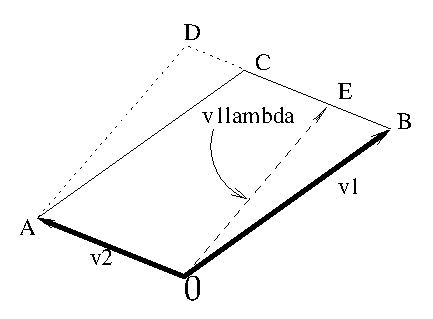
\includegraphics[width=2.2in]{v1v2-vol}
\par\end{centering}
\caption{The area of the parallelogram $0ACB$ spanned by $\left\{ \mathbf{v}_{1},\mathbf{v}_{2}\right\} $
is equal to the area of the parallelogram $0ADE$ spanned by $\left\{ \mathbf{v}_{1}+\lambda\mathbf{v}_{2},\mathbf{v}_{2}\right\} $.\label{cap:v1v2-vol}}
\end{figure}

\begin{figure}
\begin{centering}
\psfrag{apluslb}{$\mathbf{a}$} \psfrag{b}{$\mathbf{b}$} \psfrag{c}{$\mathbf{c}$} \psfrag{a}{$\mathbf{a}+\lambda\mathbf{b}$}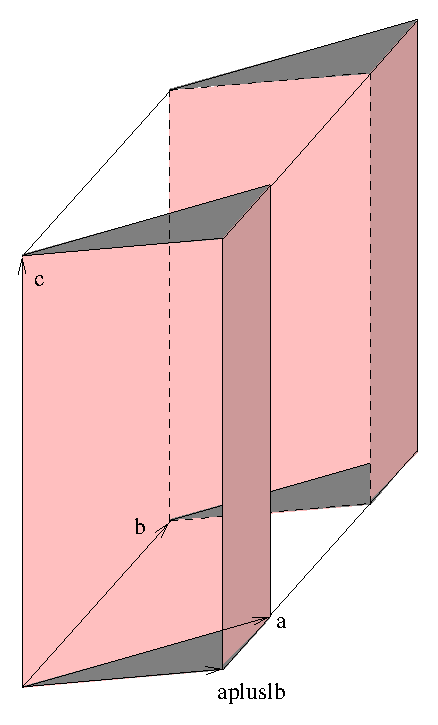
\includegraphics[width=2.2in]{3dparallelepiped_1}
\par\end{centering}
\caption{Parallelepipeds spanned by $\left\{ \mathbf{a},\mathbf{b},\mathbf{c}\right\} $
and by $\left\{ \mathbf{a}+\lambda\mathbf{b},\mathbf{b},\mathbf{c}\right\} $
have equal volume since the volumes of the shaded regions are equal.\label{fig:Parallelepipeds}}
\end{figure}


\paragraph{Proof of Statement:}

\textbf{(1)} To prove that the volumes are equal when the tensors
are equal, we will transform the first basis $\left\{ \mathbf{u}_{1},\mathbf{u}_{2},...,\mathbf{u}_{N}\right\} $
into the second basis $\left\{ \mathbf{v}_{1},\mathbf{v}_{2},...,\mathbf{v}_{N}\right\} $
by a sequence of transformations of two types: either we will multiply
one of the vectors $\mathbf{v}_{j}$ by a number $\lambda$, or add
$\lambda\mathbf{v}_{j}$ to another vector $\mathbf{v}_{k}$. We first
need to demonstrate that any basis can be transformed into any other
basis by this procedure. To demonstrate this, recall the proof of
Theorem~\ref{subsec:All-bases-have} in which vectors from the first
basis were systematically replaced by vectors of the second one. Each
replacement can be implemented by a certain sequence of replacements
of the kind $\mathbf{u}_{j}\rightarrow\lambda\mathbf{u}_{j}$ or $\mathbf{u}_{j}\rightarrow\mathbf{u}_{j}+\lambda\mathbf{u}_{i}$.
Note that the tensor $\mathbf{u}_{1}\wedge...\wedge\mathbf{u}_{N}$
changes in the same way as the volume under these replacements: The
tensor $\mathbf{u}_{1}\wedge...\wedge\mathbf{u}_{N}$ gets multiplied
by $\lambda$ after $\mathbf{u}_{j}\rightarrow\lambda\mathbf{u}_{j}$
and remains unchanged after $\mathbf{u}_{j}\rightarrow\mathbf{u}_{j}+\lambda\mathbf{u}_{i}$.
At the end of the replacement procedure, the basis $\left\{ \mathbf{u}_{j}\right\} $
becomes the basis $\left\{ \mathbf{v}_{j}\right\} $ (up to the ordering
of vectors), while the volume is multiplied by the same factor as
the tensor $\mathbf{u}_{1}\wedge...\wedge\mathbf{u}_{N}$. The ordering
of the vectors in the set $\left\{ \mathbf{v}_{j}\right\} $ can be
changed with possibly a sign change in the tensor $\mathbf{u}_{1}\wedge...\wedge\mathbf{u}_{N}$.
Therefore the statement~(\ref{eq:v1 eq v2}) is equivalent to the
assumption that the volumes of $\left\{ \mathbf{v}_{j}\right\} $
and $\left\{ \mathbf{u}_{j}\right\} $ are equal. \textbf{(2)} A transformation
$\mathbf{v}_{1}\rightarrow\lambda\mathbf{v}_{1}$ increases the volume
by a factor of $\left|\lambda\right|$ and makes the two tensors equal,
therefore the volumes differ by a factor of $\left|\lambda\right|$.\hfill{}$\blacksquare$

Let us now consider the interpretation of the above Statement. Suppose
we somehow know that the parallelepiped spanned by the vectors $\left\{ \mathbf{u}_{1},...,\mathbf{u}_{N}\right\} $
has unit volume. Given this knowledge, the volume of any other parallelepiped
spanned by some other vectors $\left\{ \mathbf{v}_{1},...,\mathbf{v}_{N}\right\} $
is easy to compute. Indeed, we can compute the tensors $\mathbf{u}_{1}\wedge...\wedge\mathbf{u}_{N}$
and $\mathbf{v}_{1}\wedge...\wedge\mathbf{v}_{N}$. Since the space
$\wedge^{N}V$ is one-dimen\-sion\-al, these two tensors must be
proportional to each other. By expanding the vectors $\mathbf{v}_{j}$
in the basis $\left\{ \mathbf{u}_{j}\right\} $, it is straightforward
to compute the coefficient $\lambda$ in the relationship
\[
\mathbf{v}_{1}\wedge...\wedge\mathbf{v}_{N}=\lambda\mathbf{u}_{1}\wedge...\wedge\mathbf{u}_{N}.
\]
The Statement now says that the volume of a parallelepiped spanned
by the vectors $\left\{ \mathbf{v}_{1},...,\mathbf{v}_{N}\right\} $
is equal to $\left|\lambda\right|$. 

\paragraph{Exercise 1:}

The volume of a parallelepiped spanned by vectors $\mathbf{a}$, $\mathbf{b}$,
$\mathbf{c}$ is equal to 19. Compute the volume of a parallelepiped
spanned by the vectors $2\mathbf{a}-\mathbf{b}$, $\mathbf{c}+3\mathbf{a}$,
$\mathbf{b}$.

\subparagraph{Solution:}

Since $\left(2\mathbf{a}-\mathbf{b}\right)\wedge\left(\mathbf{c}+3\mathbf{a}\right)\wedge\mathbf{b}=2\mathbf{a}\wedge\mathbf{c}\wedge\mathbf{b}=-2\mathbf{a}\wedge\mathbf{b}\wedge\mathbf{c}$,
the volume is 38 (twice 19; we ignored the minus sign since we are
interested only in the absolute value of the volume).\hfill{}$\blacksquare$

It is also clear that the tensor $\mathbf{v}_{1}\wedge...\wedge\mathbf{v}_{N}$
allows us only to \emph{compare} the volumes of two parallelepipeds;
we cannot determine the volume of one parallelepiped taken by itself.
A tensor such as $\mathbf{v}_{1}\wedge...\wedge\mathbf{v}_{N}$ can
be used to determine the numerical value of the volume only if we
can compare it with another given tensor, $\mathbf{u}_{1}\wedge...\wedge\mathbf{u}_{N}$,
which (\emph{by} \emph{assumption}) corresponds to a parallelepiped
of unit volume. A choice of a ``reference'' tensor $\mathbf{u}_{1}\wedge...\wedge\mathbf{u}_{N}$
can be made, for instance, if we are given a basis in $V$; without
this choice, there is no natural map from $\wedge^{N}V$ to numbers
($\mathbb{K}$). In other words, the space $\wedge^{N}V$ is \emph{not
canonically isomorphic} to the space $\mathbb{K}$ (even though both
$\wedge^{N}V$ and $\mathbb{K}$ are one-dimen\-sion\-al vector
spaces). Indeed, a canonical isomorphism between $\wedge^{N}V$ and
$\mathbb{K}$ would imply that the element $1\in\mathbb{K}$ has a
corresponding canonically defined tensor $\omega_{1}\in\wedge^{N}V$.
In that case there would be some basis $\left\{ \mathbf{e}_{j}\right\} $
in $V$ such that $\mathbf{e}_{1}\wedge...\wedge\mathbf{e}_{N}=\omega_{1}$,
which indicates that the basis $\left\{ \mathbf{e}_{j}\right\} $
is in some sense ``preferred'' or ``natural.'' However, there
is no ``natural'' or ``preferred'' choice of basis in a vector
space $V$, unless some additional structure is given (such as a scalar
product). Hence, no canonical choice of $\omega_{1}\in\wedge^{N}V$
is possible. 

\paragraph{Remark:}

When a scalar product is defined in $V$, there is a preferred choice
of basis, namely an orthonormal basis $\left\{ \mathbf{e}_{j}\right\} $
such that $\left\langle \mathbf{e}_{i},\mathbf{e}_{j}\right\rangle =\delta_{ij}$
(see Sec.~\ref{subsec:Vector-spaces-with-scalar-product}). Since
the length of each of the basis vectors is 1, and the basis vectors
are orthogonal to each other, the volume of the parallelepiped spanned
by $\left\{ \mathbf{e}_{j}\right\} $ is equal to $1$. (This is the
usual Euclidean definition of volume.) Then the tensor $\omega_{1}\equiv\bigwedge_{j=1}^{N}\mathbf{e}_{j}$
can be computed using this basis and used as a unit volume tensor.
We will see below (Sec.~\ref{proof-of-pythagoras}) that this tensor
does not depend on the choice of the orthonormal basis, up to the
orientation. The isomorphism between $\wedge^{N}V$ and $\mathbb{K}$
is then fixed (up to the sign), thanks to the scalar product.\hfill{}$\blacksquare$

In the absence of a scalar product, one can say that the \emph{value
of the volume} in an abstract vector space is not a number but a tensor
from the space $\wedge^{N}V$. It is sufficient to regard the element
$\mathbf{v}_{1}\wedge...\wedge\mathbf{v}_{N}\in\wedge^{N}V$ as the
\emph{definition} of the ``$\wedge^{N}V$-valued volume'' of the
parallelepiped spanned by $\left\{ \mathbf{v}_{j}\right\} $. The
space $\wedge^{N}V$ is one-dimen\-sion\-al, so the ``tensor-valued
volume'' has the familiar properties we expect (it is ``almost a
number''). One thing is unusual about this ``volume'': It is \textbf{oriented},
that is, it changes sign if we exchange the order of two vectors from
the set $\left\{ \mathbf{v}_{j}\right\} $. 

\paragraph{Exercise 2:}

Suppose $\left\{ \mathbf{u}_{1},...,\mathbf{u}_{N}\right\} $ is a
basis in $V$. Let $\mathbf{x}$ be some vector whose components in
the basis $\left\{ \mathbf{u}_{j}\right\} $ are given, $\mathbf{x}=\sum_{j}\alpha_{j}\mathbf{u}_{j}$.
Compute the (tensor-valued) volume of the parallelepiped spanned by
$\left\{ \mathbf{u}_{1}+\mathbf{x},...,\mathbf{u}_{N}+\mathbf{x}\right\} $.
\emph{}\\
\emph{Hints:} Use the linearity property, $\left(\mathbf{a}+\mathbf{x}\right)\wedge...=\mathbf{a}\wedge...+\mathbf{x}\wedge...$,
and notice the simplification 
\[
\mathbf{x}\wedge(\mathbf{a}+\mathbf{x})\wedge(\mathbf{b}+\mathbf{x})\wedge...\wedge(\mathbf{c}+\mathbf{x})=\mathbf{x}\wedge\mathbf{a}\wedge\mathbf{b}\wedge...\wedge\mathbf{c}.
\]


\subparagraph{Answer:}

The volume tensor is 
\[
\left(\mathbf{u}_{1}+\mathbf{x}\right)\wedge...\wedge\left(\mathbf{u}_{N}+\mathbf{x}\right)=\left(1+\alpha_{1}+...+\alpha_{N}\right)\mathbf{u}_{1}\wedge...\wedge\mathbf{u}_{N}.
\]


\paragraph{Remark: tensor-valued area\index{tensor-valued area}. }

The idea that the volume is ``oriented'' can be understood perhaps
more intuitively by considering the area of the parallelogram spanned
by two vectors $\mathbf{a}$, $\mathbf{b}$ in the familiar 3-dimen\-sion\-al
space. It is customary to draw the vector product $\mathbf{a}\times\mathbf{b}$
as the representation of this area, since the length $\left|\mathbf{a}\times\mathbf{b}\right|$
is equal to the area, and the direction of $\mathbf{a}\times\mathbf{b}$
is normal to the area. Thus, the vector $\mathbf{a}\times\mathbf{b}$
can be understood as the ``oriented area'' of the parallelogram.
However, note that the direction of the vector $\mathbf{a}\times\mathbf{b}$
depends not only on the angular orientation of the parallelogram in
space, but also on the order of the vectors $\mathbf{a}$, $\mathbf{b}$.
The 2-vector $\mathbf{a}\wedge\mathbf{b}$ is the natural analogue
of the vector product $\mathbf{a}\times\mathbf{b}$ in higher-dimen\-sion\-al
spaces. Hence, it is algebraically natural to regard the tensor $\mathbf{a}\wedge\mathbf{b}\in\wedge^{2}V$
as the ``tensor-valued'' representation of the area of the parallelogram
spanned by $\left\{ \mathbf{a},\mathbf{b}\right\} $. 

Consider now a parallelogram spanned by $\mathbf{a},\mathbf{b}$ in
a \emph{two}-dimen\-sion\-al plane. We can still represent the oriented
area of this parallelogram by the vector product $\mathbf{a}\times\mathbf{b}$,
where we imagine that the plane is embedded in a three-dimen\-sion\-al
space. The area of the parallelogram does not have a nontrivial angular
orientation any more since the vector product $\mathbf{a}\times\mathbf{b}$
is always orthogonal to the plane; the only feature left from the
orientation is the positive or negative sign of $\mathbf{a}\times\mathbf{b}$
relative to an arbitrarily chosen vector $\mathbf{n}$ normal to the
plane. Hence, we may say that the sign of the oriented volume of a
parallelepiped is the only remnant of the angular orientation of the
parallelepiped in space when the dimension of the parallelepiped is
equal to the dimension of space. (See Sec.~\ref{subsec:Motivation-for-exterior}
for more explanations about the geometrical interpretation of volume
in terms of exterior product.)\hfill{}$\blacksquare$


\section{Determinants of operators\label{subsec:The-determinant-def}}

Let $\hat{A}\in\textrm{End }V$ be a linear operator. Consider its
action on tensors from the space $\wedge^{N}V$ defined in the following
way, $\mathbf{v}_{1}\wedge...\wedge...\mathbf{v}_{N}\mapsto\hat{A}\mathbf{v}_{1}\wedge...\wedge\hat{A}\mathbf{v}_{N}$.
I denote this operation by $\wedge^{N}\hat{A}^{N}$, so 
\[
\wedge^{N}\hat{A}^{N}\left(\mathbf{v}_{1}\wedge...\wedge\mathbf{v}_{N}\right)\equiv(\hat{A}\mathbf{v}_{1})\wedge...\wedge(\hat{A}\mathbf{v}_{N}).
\]
The notation $\wedge^{N}\hat{A}^{N}$ underscores the fact that there
are $N$ copies of $\hat{A}$ acting simultaneously.

We have just defined $\wedge^{N}\hat{A}^{N}$ on single-term products
$\mathbf{v}_{1}\wedge...\wedge\mathbf{v}_{N}$; the action of $\wedge^{N}\hat{A}^{N}$
on linear combinations of such products is obtained by requiring linearity. 

Let us verify that $\wedge^{N}\hat{A}^{N}$ is a linear map; it is
sufficient to check that it is compatible with the exterior product
axioms:
\begin{align*}
\hat{A}(\mathbf{v}+\lambda\mathbf{u})\wedge\hat{A}\mathbf{v}_{2}\wedge...\wedge\hat{A}\mathbf{v}_{N} & =\hat{A}\mathbf{v}\wedge\hat{A}\mathbf{v}_{2}\wedge...\wedge\hat{A}\mathbf{v}_{N}\\
 & +\lambda\hat{A}\mathbf{u}\wedge\hat{A}\mathbf{v}_{2}\wedge...\wedge\hat{A}\mathbf{v}_{N}\;;\\
\hat{A}\mathbf{v}_{1}\wedge\hat{A}\mathbf{v}_{2}\wedge...\wedge\hat{A}\mathbf{v}_{N} & =-\hat{A}\mathbf{v}_{2}\wedge\hat{A}\mathbf{v}_{1}\wedge...\wedge\hat{A}\mathbf{v}_{N}\:.
\end{align*}
Therefore, $\wedge^{N}\hat{A}^{N}$ is now defined as a linear operator
$\wedge^{N}V\rightarrow\wedge^{N}V$.

By Theorem~2 in Sec.~\ref{subsec:Properties-of-the-ext-powers},
the space $\wedge^{N}V$ is one-dimen\-sion\-al. So $\wedge^{N}\hat{A}^{N}$,
being a linear operator in a one-dimen\-sion\-al space, must act
simply as multiplication by a number. (\emph{Every} linear operator
in a one-dimen\-sion\-al space must act as multiplication by a number!)
Thus we can write
\[
\wedge^{N}\hat{A}^{N}=\alpha\hat{1}_{\wedge^{N}V},
\]
where $\alpha\in\mathbb{K}$ is a number which is somehow associated
with the operator $\hat{A}$. What is the significance of this number
$\alpha$? This number is actually equal to the \emph{determinant}
of the operator $\hat{A}$ as given by Definition~D0. But let us
pretend that we do not know anything about determinants; it is very
convenient to use this construction to \emph{define} the determinant
and to derive its properties.

\paragraph{Definition D1:}

The \textbf{determinant}\index{determinant} $\det\hat{A}$ of an
operator $\hat{A}\in\textrm{End }V$ is the number by which any nonzero
tensor $\omega\in\wedge^{N}V$ is multiplied when $\wedge^{N}\hat{A}^{N}$
acts on it:
\begin{equation}
(\wedge^{N}\hat{A}^{N})\omega=(\det\hat{A})\omega.\label{eq:det def}
\end{equation}
In other words, $\wedge^{N}A^{N}=(\det\hat{A})\hat{1}_{\wedge^{N}V}$.

We can immediately put this definition to use; here are the first
results.

\paragraph{Statement 1:}

The determinant of a product is the product of determinants: $\det(\hat{A}\hat{B})=(\det\hat{A})(\det\hat{B})$. 

\subparagraph{Proof:}

Act with $\wedge^{N}\hat{A}^{N}$ and then with $\wedge^{N}\hat{B}^{N}$
on a nonzero tensor $\omega\in\wedge^{N}V$. Since these operators
act as multiplication by a number, the result is the multiplication
by the product of these numbers. We thus have
\[
(\wedge^{N}\hat{A}^{N})(\wedge^{N}\hat{B}^{N})\omega=(\wedge^{N}\hat{A}^{N})(\det\hat{B})\omega=(\det\hat{A})(\det\hat{B})\omega.
\]
On the other hand, for $\omega=\mathbf{v}_{1}\wedge...\wedge\mathbf{v}_{N}$
we have
\begin{align*}
(\wedge^{N}\hat{A}^{N})(\wedge^{N}\hat{B}^{N})\omega & =(\wedge^{N}\hat{A}^{N})\hat{B}\mathbf{v}_{1}\wedge...\wedge\hat{B}\mathbf{v}_{N}\\
 & =\hat{A}\hat{B}\mathbf{v}_{1}\wedge...\wedge\hat{A}\hat{B}\mathbf{v}_{N}=\wedge^{N}(\hat{A}\hat{B})^{N}\omega\\
 & =(\det(\hat{A}\hat{B}))\omega.
\end{align*}
Therefore, $\det(\hat{A}\hat{B})=(\det\hat{A})(\det\hat{B})$.\hfill{}$\blacksquare$

\paragraph{Exercise 1:}

Prove that $\det(\lambda\hat{A})=\lambda^{N}\det\hat{A}$ for any
$\lambda\in\mathbb{K}$ and $\hat{A}\in\textrm{End }V$.

Now let us clarify the relation between the determinant and the volume.
We will prove that the determinant of a transformation $\hat{A}$
is the coefficient by which the volume of parallelepipeds will grow
when we act with $\hat{A}$ on the vector space. After proving this,
I will \emph{derive} the relation~(\ref{eq:detA bad}) for the determinant
through the matrix coefficients of $\hat{A}$ in some basis; it will
follow that the formula~(\ref{eq:detA bad}) gives the same results
in any basis. 

\paragraph{Statement 2:}

When a parallelepiped spanned by the vectors $\left\{ \mathbf{v}_{1},...,\mathbf{v}_{N}\right\} $
is transformed by a linear operator $\hat{A}$, so that $\mathbf{v}_{j}\mapsto\hat{A}\mathbf{v}_{j}$,
the volume of the parallelepiped grows by the factor $|\det\hat{A}\,|$.

\subparagraph{Proof: }

Suppose the volume of the parallelepiped spanned by the vectors $\left\{ \mathbf{v}_{1},...,\mathbf{v}_{N}\right\} $
is $v$. The transformed parallelepiped is spanned by vectors $\{\hat{A}\mathbf{v}_{1},...,\hat{A}\mathbf{v}_{N}\}$.
According to the definition of the determinant, $\det\hat{A}$ is
a number such that
\[
\hat{A}\mathbf{v}_{1}\wedge...\wedge\hat{A}\mathbf{v}_{N}=(\det\hat{A})\mathbf{v}_{1}\wedge...\wedge\mathbf{v}_{N}.
\]
By Statement~\ref{subsec:The-highest-exterior}, the volume of the
transformed parallelepiped is $|\det\hat{A}\,|$ times the volume
of the original parallelepiped.\hfill{}$\blacksquare$

If we consider the oriented (i.e.~tensor-valued) volume, we find
that it grows by the factor $\det\hat{A}$ (without the absolute value).
Therefore we could define the determinant also in the following way:

\paragraph{Definition D2:}

The determinant $\det\hat{A}$ of a linear transformation $\hat{A}$
is the number by which the \emph{oriented} volume of any parallelepiped
grows after the transformation. (One is then obliged to prove that
this number does not depend on the choice of the initial parallelepiped!
We just proved this in Statement~1 using an algebraic definition
D1 of the determinant.) 

With this definition of the determinant, the property 
\[
\det(\hat{A}\hat{B})=(\det\hat{A})(\det\hat{B})
\]
 is easy to understand: The composition of the transformations $\hat{A}$
and $\hat{B}$ multiplies the volume by the product of the individual
volume growth factors $\det\hat{A}$ and $\det\hat{B}$.

Finally, here is a derivation of the formula~(\ref{eq:detA bad})
from Definition~D1.

\paragraph{Statement 3:}

If $\left\{ \mathbf{e}_{j}\right\} $ is any basis in $V$, $\left\{ \mathbf{e}_{j}^{*}\right\} $
is the dual basis, and a linear operator $\hat{A}$ is represented
by a tensor, 
\begin{equation}
\hat{A}=\sum_{j,k=1}^{N}A_{jk}\mathbf{e}_{j}\otimes\mathbf{e}_{k}^{*},\label{eq:A op as tensor}
\end{equation}
 then the determinant of $\hat{A}$ is given by the formula~(\ref{eq:detA bad}).

\subparagraph{Proof: }

The operator $\hat{A}$ defined by Eq.~(\ref{eq:A op as tensor})
acts on the basis vectors $\left\{ \mathbf{e}_{j}\right\} $ as follows,
\[
\hat{A}\mathbf{e}_{k}=\sum_{j=1}^{N}A_{jk}\mathbf{e}_{j}.
\]
 A straightforward calculation is all that is needed to obtain the
formula for the determinant. I first consider the case $N=2$ as an
illustration:
\begin{align*}
\wedge^{2}\hat{A}^{2}\left(\mathbf{e}_{1}\wedge\mathbf{e}_{2}\right) & =\hat{A}\mathbf{e}_{1}\wedge\hat{A}\mathbf{e}_{2}\\
 & =\left(A_{11}\mathbf{e}_{1}+A_{21}\mathbf{e}_{2}\right)\wedge\left(A_{12}\mathbf{e}_{1}+A_{22}\mathbf{e}_{2}\right)\\
 & =A_{11}A_{22}\mathbf{e}_{1}\wedge\mathbf{e}_{2}+A_{21}A_{12}\mathbf{e}_{2}\wedge\mathbf{e}_{1}\\
 & =\left(A_{11}A_{22}-A_{12}A_{21}\right)\mathbf{e}_{1}\wedge\mathbf{e}_{2}.
\end{align*}
Hence $\det\hat{A}=A_{11}A_{22}-A_{12}A_{21}$, in agreement with
the usual formula.

Now I consider the general case. The action of $\wedge^{N}\hat{A}^{N}$
on the basis element $\mathbf{e}_{1}\wedge...\wedge\mathbf{e}_{N}\in\wedge^{N}V$
is
\begin{align}
\wedge^{N}\hat{A}^{N}\left(\mathbf{e}_{1}\wedge...\wedge\mathbf{e}_{N}\right) & =\hat{A}\mathbf{e}_{1}\wedge...\wedge\hat{A}\mathbf{e}_{N}\nonumber \\
=\left(\sum_{j_{1}=1}^{N}A_{j_{1}1}\mathbf{e}_{j_{1}}\right) & \wedge...\wedge\left(\sum_{j_{N}=1}^{N}A_{j_{N}N}\mathbf{e}_{j_{N}}\right)\nonumber \\
=\sum_{j_{1}=1}^{N}...\sum_{j_{N}=1}^{N} & A_{j_{1}1}\mathbf{e}_{j_{1}}\wedge...\wedge A_{j_{N}N}\mathbf{e}_{j_{N}}\nonumber \\
=\sum_{j_{1}=1}^{N}...\sum_{j_{N}=1}^{N} & (A_{j_{1}1}...A_{j_{N}N})\mathbf{e}_{j_{1}}\wedge...\wedge\mathbf{e}_{j_{N}}.\label{eq:last permutation}
\end{align}
In the last sum, the only nonzero terms are those in which the indices
$j_{1}$, ..., $j_{N}$ do not repeat; in other words, $\left(j_{1},...,j_{N}\right)$
is a \emph{permutation} of the set (1, ..., $N$). Let us therefore
denote this permutation by $\sigma$ and write $\sigma(1)\equiv j_{1}$,
..., $\sigma(N)\equiv j_{N}$. Using the antisymmetry of the exterior
product and the definition of the parity $\left|\sigma\right|$ of
the permutation $\sigma$, we can express
\[
\mathbf{e}_{j_{1}}\wedge...\wedge\mathbf{e}_{j_{N}}=\mathbf{e}_{\sigma(1)}\wedge...\wedge\mathbf{e}_{\sigma(N)}=\left(-1\right)^{\left|\sigma\right|}\mathbf{e}_{1}\wedge...\wedge\mathbf{e}_{N}.
\]
Now we can rewrite the last line in Eq.~(\ref{eq:last permutation})
in terms of sums over all permutations $\sigma$ instead of sums over
all $\left\{ j_{1},...,j_{N}\right\} $: 
\begin{align*}
\wedge^{N}\hat{A}^{N}\left(\mathbf{e}_{1}\wedge...\wedge\mathbf{e}_{N}\right)= & \sum_{\sigma}A_{\sigma(1)1}...A_{\sigma(N)N}\mathbf{e}_{\sigma(1)}\wedge...\wedge\mathbf{e}_{\sigma(N)}\\
=\sum_{\sigma}A_{\sigma(1)1}...A_{\sigma(N)N} & \left(-1\right)^{\left|\sigma\right|}\mathbf{e}_{1}\wedge...\wedge\mathbf{e}_{N}.
\end{align*}
Thus we have reproduced the formula~(\ref{eq:detA bad}).\hfill{}$\blacksquare$

We have seen three equivalent definitions of the determinant, each
with its own advantages: first, a direct but complicated definition~(\ref{eq:detA bad})
in terms of matrix coefficients; second, an elegant but abstract definition~(\ref{eq:det def})
that depends on the construction of the exterior product; third, an
intuitive and visual definition in terms of the volume which, however,
is based on the geometric notion of ``volume of an $N$-dimen\-sion\-al
domain'' rather than on purely algebraic constructions. All three
definitions are equivalent when applied to linear operators in finite-dimen\-sion\-al
spaces.

\subsection{Examples: computing  determinants}

\paragraph{Question:}

We have been working with operators more or less in the same way as
with matrices, like in Eq.~(\ref{eq:A op as tensor}). What is the
advantage of the coord\-in\-ate-free approach if we are again computing
with the elements of matrices?

\subparagraph{Answer:}

In some cases, there is no other way except to represent an operator
in some basis through a matrix such as $A_{ij}$. However, in many
cases an interesting operator can be represented \emph{geometrically},
i.e.~without choosing a basis. It is often useful to express an operator
in a basis-free manner because this yields some nontrivial information
that would otherwise be obscured by an unnecessary (or wrong) choice
of basis. It is useful to be able to employ both the basis-free and
the component-based techniques. Here are some examples where we compute
determinants of operators defined without a basis.

\paragraph{Example 1:}

Operators of the form $\hat{1}_{V}+\mathbf{a}\otimes\mathbf{b}^{*}$
are useful in geometry because they can represent reflections or projections
with respect to an axis or a plane if $\mathbf{a}$ and $\mathbf{b}^{*}$
are chosen appropriately. For instance, if $\mathbf{b}^{*}\neq0$,
we can define a \textbf{hyperplane}\index{hyperplane} $H_{\mathbf{b}^{*}}\subset V$
as the subspace annihilated by the covector $\mathbf{b}^{*}$, i.e.~the
subspace consisting of vectors $\mathbf{v}\in V$ such that $\mathbf{b}^{*}\left(\mathbf{v}\right)=0$.
If a vector $\mathbf{a}\in V$ is such that $\mathbf{b}^{*}\left(\mathbf{a}\right)\neq0$,
i.e.~$\mathbf{a}\not\in H_{\mathbf{b}^{*}}$, then 
\[
\hat{P}\equiv\hat{1}_{V}-\frac{1}{\mathbf{b}^{*}\left(\mathbf{a}\right)}\mathbf{a}\otimes\mathbf{b}^{*}
\]
is a projector\index{projector} onto $H_{\mathbf{b}^{*}}$, while
the operator
\[
\hat{R}\equiv\hat{1}_{V}-\frac{2}{\mathbf{b}^{*}\left(\mathbf{a}\right)}\mathbf{a}\otimes\mathbf{b}^{*}
\]
describes a \textbf{mirror} \textbf{reflection}\index{mirror reflection}
with respect to the hyperplane $H_{\mathbf{b}^{*}}$, in the sense
that $\mathbf{v}+\hat{R}\mathbf{v}\in H_{\mathbf{b}^{*}}$ for any
$\mathbf{v}\in V$.\hfill{}$\blacksquare$

The following statement shows how to calculate determinants of such
operators. For instance, with the above definitions we would find
$\det\hat{P}=0$ and $\det\hat{R}=-1$ by a direct application of
Eq.~(\ref{eq:det lambda ab}).

\paragraph{Statement: }

Let $\mathbf{a}\in V$ and $\mathbf{b}^{*}\in V^{*}$. Then
\begin{equation}
\det\left(\hat{1}_{V}+\mathbf{a}\otimes\mathbf{b}^{*}\right)=1+\mathbf{b}^{*}\left(\mathbf{a}\right).\label{eq:det lambda ab}
\end{equation}


\subparagraph{Proof:}

If $\mathbf{b}^{*}=0$, the formula is trivial, so we assume that
$\mathbf{b}^{*}\neq0$. Then we need to consider two cases: $\mathbf{b}^{*}(\mathbf{a})\neq0$
or $\mathbf{b}^{*}(\mathbf{a})=0$; however, the final formula~(\ref{eq:det lambda ab})
is the same in both cases. 

Case 1. By Statement~\ref{subsec:Dual-vector-space}, if $\mathbf{b}^{*}\left(\mathbf{a}\right)\neq0$
there exists a basis $\left\{ \mathbf{a},\mathbf{v}_{2},...,\mathbf{v}_{N}\right\} $
such that $\mathbf{b}^{*}\left(\mathbf{v}_{i}\right)=0$ for $2\leq i\leq N$,
where $N=\dim V$. Then we compute the determinant by applying the
operator $\wedge^{N}\left(\hat{1}_{V}+\mathbf{a}\otimes\mathbf{b}^{*}\right)^{N}$
to the tensor $\mathbf{a}\wedge\mathbf{v}_{2}\wedge...\wedge\mathbf{v}_{N}$:
since
\begin{align*}
\left(\hat{1}_{V}+\mathbf{a}\otimes\mathbf{b}^{*}\right)\mathbf{a} & =\left(1+\mathbf{b}^{*}\left(\mathbf{a}\right)\right)\mathbf{a},\\
\left(\hat{1}_{V}+\mathbf{a}\otimes\mathbf{b}^{*}\right)\mathbf{v}_{i} & =\mathbf{v}_{i},\quad i=2,...,N,
\end{align*}
we get
\begin{align*}
\wedge^{N}\left(\hat{1}_{V}+\mathbf{a}\otimes\mathbf{b}^{*}\right)^{N}\mathbf{a}\wedge\mathbf{v}_{2}\wedge...\wedge\mathbf{v}_{N}\\
=\left(1+\mathbf{b}^{*}\left(\mathbf{a}\right)\right)\mathbf{a}\wedge\mathbf{v}_{2}\wedge...\wedge\mathbf{v}_{N}.
\end{align*}
Therefore $\det\left(\hat{1}_{V}+\mathbf{a}\otimes\mathbf{b}^{*}\right)=1+\mathbf{b}^{*}\left(\mathbf{a}\right)$,
as required.

Case 2. If $\mathbf{b}^{*}\left(\mathbf{a}\right)=0$, we will show
that $\det\left(\hat{1}_{V}+\mathbf{a}\otimes\mathbf{b}^{*}\right)=1$.
We cannot choose the basis $\left\{ \mathbf{a},\mathbf{v}_{2},...,\mathbf{v}_{N}\right\} $
as in case 1, so we need to choose another basis. There exists some
vector $\mathbf{w}\in V$ such that $\mathbf{b}^{*}\left(\mathbf{w}\right)\neq0$
because by assumption $\mathbf{b}^{*}\neq0$. It is clear that $\left\{ \mathbf{w},\mathbf{a}\right\} $
is a linearly independent set: otherwise we would have $\mathbf{b}^{*}(\mathbf{w})=0$.
Therefore, we can complete this set to a basis $\left\{ \mathbf{w},\mathbf{a},\mathbf{v}_{3},...,\mathbf{v}_{N}\right\} $.
Further, the vectors $\mathbf{v}_{3},...,\mathbf{v}_{N}$ can be chosen
such that $\mathbf{b}^{*}\left(\mathbf{v}_{i}\right)=0$ for $3\leq i\leq N$.
Now we compute the determinant by acting with the operator $\wedge^{N}\left(\hat{1}_{V}+\mathbf{a}\otimes\mathbf{b}^{*}\right)^{N}$
on the tensor $\mathbf{a}\wedge\mathbf{w}\wedge\mathbf{v}_{3}\wedge...\wedge\mathbf{v}_{N}$:
since
\begin{align*}
\left(\hat{1}_{V}+\mathbf{a}\otimes\mathbf{b}^{*}\right)\mathbf{a} & =\mathbf{a},\\
\left(\hat{1}_{V}+\mathbf{a}\otimes\mathbf{b}^{*}\right)\mathbf{w} & =\mathbf{w}+\mathbf{b}^{*}\left(\mathbf{w}\right)\mathbf{a},\\
\left(\hat{1}_{V}+\mathbf{a}\otimes\mathbf{b}^{*}\right)\mathbf{v}_{i} & =\mathbf{v}_{i},\quad i=3,...,N,
\end{align*}
we get
\begin{align*}
\wedge^{N}\left(\hat{1}_{V}+\mathbf{a}\otimes\mathbf{b}^{*}\right)^{N}\mathbf{a}\wedge\mathbf{w}\wedge\mathbf{v}_{3}\wedge...\wedge\mathbf{v}_{N}\\
=\mathbf{a}\wedge\left(\mathbf{w}+\mathbf{b}^{*}\left(\mathbf{w}\right)\mathbf{a}\right)\wedge\mathbf{v}_{3}\wedge...\wedge\mathbf{v}_{N}\\
=\mathbf{a}\wedge\mathbf{w}\wedge\mathbf{v}_{3}\wedge...\wedge\mathbf{v}_{N}.
\end{align*}
Therefore $\det\left(\hat{1}_{V}+\mathbf{a}\otimes\mathbf{b}^{*}\right)=1$.\hfill{}$\blacksquare$

\paragraph{Exercise 1: }

In a similar way, prove the following statement: If $\mathbf{a}_{i}\in V$
and $\mathbf{b}_{i}^{*}\in V^{*}$ for $1\leq i\leq n<N$ are such
that $\mathbf{b}_{i}^{*}\left(\mathbf{a}_{j}\right)=0$ for all $i>j$,
then
\[
\det\,\bigg(\hat{1}_{V}+\sum_{i=1}^{n}\mathbf{a}_{i}\otimes\mathbf{b}_{i}^{*}\bigg)\,=\prod_{i=1}^{n}\left(1+\mathbf{b}_{i}^{*}\left(\mathbf{a}_{i}\right)\right).
\]


\paragraph{Exercise 2: }

Consider the three-dimen\-sion\-al space of polynomials $p(x)$
in the variable $x$ of degree at most 2 with real coefficients. The
operators $\hat{A}$ and $\hat{B}$ are defined by 
\begin{align*}
(\hat{A}p)(x) & \equiv p(x)+x\frac{dp(x)}{dx},\\
(\hat{B}p)(x) & \equiv x^{2}p(1)+2p(x).
\end{align*}
Check that these operators are linear. Compute the determinants of
$\hat{A}$ and $\hat{B}$.

\subparagraph{Solution: }

The operators are linear because they are expressed as formulas containing
$p(x)$ linearly. Let us use the underbar to distinguish the polynomials
$\underbar{1}$, $\underbar{x}$ from numbers such as 1. A convenient
basis tensor of the 3rd exterior power is $\underbar{1}\wedge\underbar{x}\wedge\underbar{x}^{2}$,
so we perform the calculation, 
\begin{align*}
(\det\hat{A})(\underbar{1}\wedge\underbar{x}\wedge\underbar{x}^{2}) & =(\hat{A}\underbar{1})\wedge(\hat{A}\underbar{x})\wedge(\hat{A}\underbar{x}^{2})\\
=\underbar{1}\wedge(2\underbar{x})\wedge(3\underbar{x}^{2}) & =6(\underbar{1}\wedge\underbar{x}\wedge\underbar{x}^{2}),
\end{align*}
and find that $\det\hat{A}=6$. Similarly we find $\det\hat{B}=12$.\hfill{}$\blacksquare$

\paragraph{Exercise 3:}

Suppose the space $V$ is decomposed into a direct sum of $U$ and
$W$, and an operator $\hat{A}$ is such that $U$ and $W$ are invariant
subspaces ($\hat{A}\mathbf{x}\in U$ for all $\mathbf{x}\in U$, and
the same for $W$). Denote by $\hat{A}_{U}$ the restriction of the
operator $\hat{A}$ to the subspace $U$. Show that
\[
\det\hat{A}=(\det\hat{A}_{U})(\det\hat{A}_{W}).
\]

\emph{Hint}: Choose a basis in $V$ as the union of a basis in $U$
and a basis in $W$. In this basis, the operator $\hat{A}$ is represented
by a \textbf{block-diagonal\index{block-diagonal matrix}} matrix.

\section{Determinants of square tables\label{subsec:Determinants-of-square}}

Note that the determinant formula~(\ref{eq:detA bad}) applies to
\emph{any} square matrix, without referring to any transformations
in any vector spaces. Sometimes it is useful to compute the determinants
of matrices that do not represent linear transformations. Such matrices
are really just \emph{tables of numbers}. The properties of determinants
of course remain the same whether or not the matrix represents a linear
transformation in the context of the problem we are solving. The geometric
construction of the determinant through the space $\wedge^{N}V$ is
useful because it helps us understand heuristically where the properties
of the determinant come from. 

Given just a square table of numbers, it is often useful to \emph{introduce}
a linear transformation corresponding to the matrix in some (conveniently
chosen) basis; this often helps solve problems. An example frequently
used in linear algebra is a matrix consisting of the components of
some vectors in a basis. Suppose $\left\{ \mathbf{e}_{j}\,|\,j=1,...,N\right\} $
is a basis and $\left\{ \mathbf{v}_{j}\,|\,j=1,...,N\right\} $ are
some vectors. Since each of the $\mathbf{v}_{j}$ can be decomposed
through the basis $\left\{ \mathbf{e}_{j}\right\} $, say 
\[
\mathbf{v}_{i}=\sum_{j=1}^{N}v_{ij}\mathbf{e}_{j},\quad i=1,...,N,
\]
we may consider the coefficients $v_{ij}$ as a square matrix. This
matrix, at first glance, does not represent a linear transformation;
it's just a square-shaped table of the coefficients $v_{ij}$. However,
let us \emph{define} a linear operator $\hat{A}$ by the condition
that $\hat{A}\mathbf{e}_{i}=\mathbf{v}_{i}$ for all $i=1,...,N$.
This condition defines $\hat{A}\mathbf{x}$ for any vector $\mathbf{x}$
if we assume the linearity of $\hat{A}$ (see Exercise~2 in Sec.~\ref{subsec:Examples-of-linear-maps}).
The operator $\hat{A}$ has the following matrix representation with
respect to the basis $\left\{ \mathbf{e}_{i}\right\} $ and the dual
basis $\left\{ \mathbf{e}_{i}^{*}\right\} $:
\[
\hat{A}=\sum_{i=1}^{N}\mathbf{v}_{i}\otimes\mathbf{e}_{i}^{*}=\sum_{i=1}^{N}\sum_{j=1}^{N}v_{ij}\mathbf{e}_{j}\otimes\mathbf{e}_{i}^{*}.
\]
So the matrix $v_{ji}$ (the transpose of $v_{ij}$) is the matrix
representing the transformation $\hat{A}$. Let us consider the determinant
of this transformation:
\[
(\det\hat{A})\mathbf{e}_{1}\wedge...\wedge\mathbf{e}_{N}=\hat{A}\mathbf{e}_{1}\wedge...\wedge\hat{A}\mathbf{e}_{N}=\mathbf{v}_{1}\wedge...\wedge\mathbf{v}_{N}.
\]
The determinant of the matrix $v_{ji}$ is thus equal to the determinant
of the transformation $\hat{A}$. Hence, the computation of the determinant
of the matrix $v_{ji}$ is equivalent to the computation of the tensor
$\mathbf{v}_{1}\wedge...\wedge\mathbf{v}_{N}\in\wedge^{N}V$ and its
comparison with the basis tensor $\mathbf{e}_{1}\wedge...\wedge\mathbf{e}_{N}$.
We have thus proved the following statement.

\paragraph{Statement 1: }

The determinant\index{determinant} of the matrix $v_{ji}$ made up
by the components of the vectors $\left\{ \mathbf{v}_{j}\right\} $
in a basis $\left\{ \mathbf{e}_{j}\right\} $ ($j=1,...,N$) is the
number $C$ defined as the coefficient in the tensor equality
\[
\mathbf{v}_{1}\wedge...\wedge\mathbf{v}_{N}=C\mathbf{e}_{1}\wedge...\wedge\mathbf{e}_{N}.
\]


\paragraph{Corollary:}

The determinant of a matrix does not change when a multiple of one
row is added to another row. The determinant is linear as a function
of each row. The determinant changes sign when two rows are exchanged.

\subparagraph{Proof:}

We consider the matrix $v_{ij}$ as the table of coefficients of vectors
$\left\{ \mathbf{v}_{j}\right\} $ in a basis $\left\{ \mathbf{e}_{j}\right\} $,
as explained above. Since
\[
(\det v_{ji})\mathbf{e}_{1}\wedge...\wedge\mathbf{e}_{N}=\mathbf{v}_{1}\wedge...\wedge\mathbf{v}_{N},
\]
we need only to examine the properties of the tensor $\omega\equiv\mathbf{v}_{1}\wedge...\wedge\mathbf{v}_{N}$
under various replacements. When a multiple of row $k$ is added to
another row $j$, we replace $\mathbf{v}_{j}\mapsto\mathbf{v}_{j}+\lambda\mathbf{v}_{k}$
for fixed $j,k$; then the tensor $\omega$ does not change,
\[
\mathbf{v}_{1}\wedge...\wedge\mathbf{v}_{j}\wedge...\wedge\mathbf{v}_{N}=\mathbf{v}_{1}\wedge...\wedge\left(\mathbf{v}_{j}+\lambda\mathbf{v}_{k}\right)\wedge...\wedge\mathbf{v}_{N},
\]
 hence the determinant of $v_{ij}$ does not change. To show that
the determinant is linear as a function of each row, we consider the
replacement $\mathbf{v}_{j}\mapsto\mathbf{u}+\lambda\mathbf{v}$ for
fixed $j$; the tensor $\omega$ is then equal to the sum of the tensors
$\mathbf{v}_{1}\wedge...\wedge\mathbf{u}\wedge...\wedge\mathbf{v}_{N}$
and $\lambda\mathbf{v}_{1}\wedge...\wedge\mathbf{v}\wedge...\wedge\mathbf{v}_{N}$.
Finally, exchanging the rows $k$ and $l$ in the matrix $v_{ij}$
corresponds to exchanging the vectors $\mathbf{v}_{k}$ and $\mathbf{v}_{l}$,
and then the tensor $\omega$ changes sign.\hfill{}$\blacksquare$

It is an important property that matrix transposition leaves the determinant
unchanged.

\paragraph{Statement 2:}

The determinant of the transposed operator is unchanged: 
\[
\det\hat{A}^{T}=\det\hat{A}.
\]


\subparagraph{Proof:}

I give two proofs, one based on Definition~D0 and the properties
of permutations, another entirely coordinate-free --- based on Definition~D1
of the determinant and definition~\ref{par:Definition:transpose}
of the transposed operator.

\emph{First proof}: According to Definition~D0, the determinant of
the transposed matrix $A_{ji}$ is given by the formula 
\begin{equation}
\det(A_{ji})\equiv\sum_{\sigma}\left(-1\right)^{\left|\sigma\right|}A_{1,\sigma(1)}...A_{N,\sigma(N)},\label{eq:det transpose 0}
\end{equation}
so the only difference between $\det(A_{ij})$ and $\det(A_{ji})$
is the order of indices in the products of matrix elements, namely
$A_{\sigma(i),i}$ instead of $A_{i,\sigma(i)}$. We can show that
the sum in Eq.~(\ref{eq:det transpose 0}) consists of exactly the
same terms as the sum in Eq.~(\ref{eq:detA bad}), only the terms
occur in a different order. This is sufficient to prove that $\det(A_{ij})=\det(A_{ji})$.

The sum in Eq.~(\ref{eq:det transpose 0}) consists of terms of the
form $A_{1,\sigma(1)}...A_{N,\sigma(N)}$, where $\sigma$ is some
permutation. We may reorder factors in this term,
\[
A_{1,\sigma(1)}...A_{N,\sigma(N)}=A_{\sigma^{\prime}(1),1}...A_{\sigma^{\prime}(N),N},
\]
where $\sigma'$ is another permutation such that $A_{i,\sigma(i)}=A_{\sigma^{\prime}(i),i}$
for $i=1,...,N$. This is achieved when $\sigma'$ is the permutation
inverse to $\sigma$, i.e.~we need to use $\sigma^{\prime}\equiv\sigma^{-1}$.
Since there exists precisely one inverse permutation $\sigma^{-1}$
for each permutation $\sigma$, we may transform the sum in Eq.~(\ref{eq:det transpose 0})
into a sum over all inverse permutations $\sigma'$; each permutation
will still enter exactly once into the new sum. Since the parity of
the inverse permutation $\sigma^{-1}$ is the same as the parity of
$\sigma$ (see Statement~3 in Appendix~\ref{subsec:Properties-of-permutations}),
the factor $\left(-1\right)^{|\sigma|}$ will remain unchanged. Therefore,
the sum will remain the same.

\emph{Second proof}: The transposed operator is defined as
\[
(\hat{A}^{T}\mathbf{f}^{*})(\mathbf{x})=\mathbf{f}^{*}(\hat{A}\mathbf{x}),\quad\forall\mathbf{f}^{*}\in V^{*},\;\mathbf{x}\in V.
\]
In order to compare the determinants $\det\hat{A}$ and $\det(\hat{A}^{T})$
according to Definition~D1, we need to compare the numbers $\wedge^{N}\hat{A}^{N}$
and $\wedge^{N}(\hat{A}^{T})^{N}$. 

Let us choose nonzero tensors $\omega\in\wedge^{N}V$ and $\omega^{*}\in\wedge^{N}V^{*}$.
By Lemma~1 in Sec.~\ref{subsec:Properties-of-the-ext-powers}, these
tensors have representations of the form $\omega=\mathbf{v}_{1}\wedge...\wedge\mathbf{v}_{N}$
and $\omega^{*}=\mathbf{f}_{1}^{*}\wedge...\wedge\mathbf{f}_{N}^{*}$.
We have 
\[
(\det\hat{A})\mathbf{v}_{1}\wedge...\wedge\mathbf{v}_{N}=\hat{A}\mathbf{v}_{1}\wedge...\wedge\hat{A}\mathbf{v}_{N}.
\]
Now we would like to relate this expression with the analogous expression
for $\hat{A}^{T}$. In order to use the definition of $\hat{A}^{T}$,
we need to act on the vectors $\hat{A}\mathbf{v}_{i}$ by the covectors
$\mathbf{f}_{j}^{*}$. Therefore, we act with the $N$-form $\omega^{*}\in\wedge^{N}V^{*}\cong(\wedge^{N}V)^{*}$
on the $N$-vector $\wedge^{N}\hat{A}^{N}\omega\in\wedge^{N}V$ (this
canonical action was defined by Definition~3 in Sec.~\ref{subsec:Definition-of-the-exterior}).
Since this action is linear, we find
\[
\omega^{*}(\wedge^{N}\hat{A}^{N}\omega)=(\det\hat{A})\omega^{*}(\omega).
\]
(Note that $\omega^{*}(\omega)\neq0$ since by assumption the tensors
$\omega$ and $\omega^{*}$ are nonzero.) On the other hand, 
\begin{align*}
\omega^{*}\big({\wedge^{N}\hat{A}^{N}}\omega\big) & =\sum_{\sigma}(-1)^{\left|\sigma\right|}\mathbf{f}_{1}^{*}(\hat{A}\mathbf{v}_{\sigma(1)})...\mathbf{f}_{N}^{*}(\hat{A}\mathbf{v}_{\sigma(N)})\\
 & =\sum_{\sigma}(-1)^{\left|\sigma\right|}(\hat{A}^{T}\mathbf{f}_{1}^{*})(\mathbf{v}_{\sigma(1)})...(\hat{A}^{T}\mathbf{f}_{N}^{*})(\mathbf{v}_{\sigma(N)})\\
 & =\big({\wedge^{N}(\hat{A}^{T})^{N}}\omega^{*}\big)(\omega)=(\det\hat{A}^{T})\omega^{*}(\omega).
\end{align*}
Hence $\det\hat{A}^{T}=\det\hat{A}$.\hfill{}$\blacksquare$

\paragraph{Exercise{*} (Laplace expansion\index{Laplace expansion}):}

As shown in the Corollary above, the determinant of the matrix $v_{ij}$
is a linear function of each of the vectors $\left\{ \mathbf{v}_{i}\right\} $.
Consider $\det(v_{ij})$ as a linear function of the first vector,
$\mathbf{v}_{1}$; this function is a \emph{covector} that we may
temporarily denote by $\mathbf{f}_{1}^{*}$. Show that $\mathbf{f}_{1}^{*}$
can be represented in the dual basis $\left\{ \mathbf{e}_{j}^{*}\right\} $
as
\[
\mathbf{f}_{1}^{*}=\sum_{i=1}^{N}\left(-1\right)^{i-1}B_{1i}\mathbf{e}_{i}^{*},
\]
where the coefficients $B_{1i}$ are \textbf{minors}\index{minor}
of the matrix $v_{ij}$, that is, determinants of the matrix $v_{ij}$
from which row 1 and column $i$ have been deleted.

\subparagraph{Solution:}

Consider one of the coefficients, for example $B_{11}\equiv\mathbf{f}_{1}^{*}(\mathbf{e}_{1})$.
This coefficient can be determined from the tensor equality
\begin{equation}
\mathbf{e}_{1}\wedge\mathbf{v}_{2}\wedge...\wedge\mathbf{v}_{N}=B_{11}\mathbf{e}_{1}\wedge...\wedge\mathbf{e}_{N}.\label{eq:laplace}
\end{equation}
We could reduce $B_{11}$ to a determinant of an $(N-1)\times(N-1)$
matrix if we could cancel $\mathbf{e}_{1}$ on both sides of Eq.~(\ref{eq:laplace}).
We would be able to cancel $\mathbf{e}_{1}$ if we had a tensor equality
of the form 
\[
\mathbf{e}_{1}\wedge\psi=B_{11}\mathbf{e}_{1}\wedge\mathbf{e}_{2}\wedge...\wedge\mathbf{e}_{N},
\]
 where the ($N-1$)-vector $\psi$ were proportional to $\mathbf{e}_{2}\wedge...\wedge\mathbf{e}_{N}$.
However, $\mathbf{v}_{2}\wedge...\wedge\mathbf{v}_{N}$ in Eq.~(\ref{eq:laplace})
is not necessarily proportional to $\mathbf{e}_{2}\wedge...\wedge\mathbf{e}_{N}$;
so we need to transform Eq.~(\ref{eq:laplace}) to a suitable form.
In order to do this, we transform the vectors $\mathbf{v}_{i}$ into
vectors that belong to the subspace spanned by $\left\{ \mathbf{e}_{2},...,\mathbf{e}_{N}\right\} $.
We subtract from each $\mathbf{v}_{i}$ ($i=2,...,N$) a suitable
multiple of $\mathbf{e}_{1}$ and define the vectors $\tilde{\mathbf{v}}_{i}$
($i=2,...,N$) such that $\mathbf{e}_{1}^{*}(\tilde{\mathbf{v}}_{i})=0$:
\[
\tilde{\mathbf{v}}_{i}\equiv\mathbf{v}_{i}-\mathbf{e}_{1}^{*}(\mathbf{v}_{i})\mathbf{e}_{1},\quad i=2,...,N.
\]
Then $\tilde{\mathbf{v}}_{i}\in\text{Span}\left\{ \mathbf{e}_{2},...,\mathbf{e}_{N}\right\} $
and also 
\[
\mathbf{e}_{1}\wedge\mathbf{v}_{2}\wedge...\wedge\mathbf{v}_{N}=\mathbf{e}_{1}\wedge\tilde{\mathbf{v}}_{2}\wedge...\wedge\tilde{\mathbf{v}}_{N}.
\]
 Now Eq.~(\ref{eq:laplace}) is rewritten as
\[
\mathbf{e}_{1}\wedge\tilde{\mathbf{v}}_{2}\wedge...\wedge\tilde{\mathbf{v}}_{N}=B_{11}\mathbf{e}_{1}\wedge\mathbf{e}_{2}\wedge...\wedge\mathbf{e}_{N}.
\]
Since $\tilde{\mathbf{v}}_{i}\in\text{Span}\left\{ \mathbf{e}_{2},...,\mathbf{e}_{N}\right\} $,
the tensors $\tilde{\mathbf{v}}_{2}\wedge...\wedge\tilde{\mathbf{v}}_{N}$
and $\mathbf{e}_{2}\wedge...\wedge\mathbf{e}_{N}$ are proportional
to each other. Now we are allowed to cancel $\mathbf{e}_{1}$ and
obtain 
\[
\tilde{\mathbf{v}}_{2}\wedge...\wedge\tilde{\mathbf{v}}_{N}=B_{11}\mathbf{e}_{2}\wedge...\wedge\mathbf{e}_{N}.
\]
Note that the vectors $\tilde{\mathbf{v}}_{i}$ have the first components
equal to zero. In other words, $B_{11}$ is equal to the determinant
of the matrix $v_{ij}$ from which row 1 (i.e.~the vector $\mathbf{v}_{1}$)
and column 1 (the coefficients at $\mathbf{e}_{1}$) have been deleted.
The coefficients $B_{1j}$ for $j=2,...,N$ are calculated similarly.\hfill{}$\blacksquare$

\subsection{{*} Index notation for $\wedge^{N}V$ and determinants\label{subsec:Index-notation-for-determinants}}

Let us see how determinants are written in the index notation.

In order to use the index notation, we need to fix a basis $\left\{ \mathbf{e}_{j}\right\} $
and represent each vector and each tensor by their components in that
basis. Determinants are related to the space $\wedge^{N}V$. Let us
consider a set of vectors $\{\mathbf{v}_{1},...,\mathbf{v}_{N}\}$
and the tensor 
\[
\psi\equiv\mathbf{v}_{1}\wedge...\wedge\mathbf{v}_{N}\in\wedge^{N}V.
\]
Since the space $\wedge^{N}V$ is one-dimen\-sion\-al and its basis
consists of the single tensor $\mathbf{e}_{1}\wedge...\wedge\mathbf{e}_{N}$,
the index representation of $\psi$ consists, in principle, of the
single number $C$ in a formula such as
\[
\psi=C\mathbf{e}_{1}\wedge...\wedge\mathbf{e}_{N}.
\]
 However, it is more convenient to use a totally antisymmetric array
of numbers having $N$ indices, $\psi^{i_{1}...i_{N}}$, so that
\[
\psi=\frac{1}{N!}\sum_{i_{1},...,i_{N}=1}^{N}\psi^{i_{1}...i_{N}}\mathbf{e}_{i_{1}}\wedge...\wedge\mathbf{e}_{i_{N}}.
\]
Then the coefficient $C$ is $C\equiv\psi^{12...N}$. In the formula
above, the combinatorial factor $N!$ compensates the fact that we
are summing an antisymmetric product of vectors with a totally antisymmetric
array of coefficients. 

To write such arrays more conveniently, one can use Levi-Civita symbol
$\varepsilon^{i_{1}...i_{N}}$ (see Sec.~\ref{subsec:Exterior-product-in-index}).\index{Levi-Civita symbol}
It is clear that any other totally antisymmetric array of numbers
with $N$ indices, such as $\psi^{i_{1}...i_{N}}$, is proportional
to $\varepsilon^{i_{1}...i_{N}}$: For indices $\left\{ i_{1},...,i_{N}\right\} $
that correspond to a permutation $\sigma$ we have 
\[
\psi^{i_{1}...i_{N}}=\psi^{12...N}(-1)^{\left|\sigma\right|},
\]
and hence
\[
\psi^{i_{1}...i_{N}}=(\psi^{12...N})\varepsilon^{i_{1}...i_{N}}.
\]

How to compute the index representation of $\psi$ given the array
$v_{j}^{k}$ of the components of the vectors $\left\{ \mathbf{v}_{j}\right\} $?
We need to represent the tensor 
\[
\psi\equiv\sum_{\sigma}\left(-1\right)^{\left|\sigma\right|}\mathbf{v}_{\sigma(1)}\otimes\mathbf{v}_{\sigma(2)}\otimes...\otimes\mathbf{v}_{\sigma(N)}.
\]
Hence, we can use the Levi-Civita symbol and write
\begin{align*}
\psi^{12...N} & =\sum_{\sigma}\left(-1\right)^{\left|\sigma\right|}v_{\sigma(1)}^{1}\otimes v_{\sigma(2)}^{2}\otimes...\otimes v_{\sigma(N)}^{N}\\
 & =\sum_{i_{1},...,i_{N}=1}^{N}\varepsilon^{i_{1}...i_{N}}v_{i_{1}}^{1}...v_{i_{N}}^{N}.
\end{align*}
The component $\psi^{12...N}$ is the only number we need to represent
$\psi$ in the basis $\left\{ \mathbf{e}_{j}\right\} $.

The Levi-Civita symbol itself can be seen as the index representation
of the tensor 
\[
\omega\equiv\mathbf{e}_{1}\wedge...\wedge\mathbf{e}_{N}
\]
 in the basis $\left\{ \mathbf{e}_{j}\right\} $. (The components
of $\omega$ in a different basis will, of course, differ from $\varepsilon^{i_{1}...i_{N}}$
by a constant factor.)

Now let us construct the index representation of the determinant of
an operator $\hat{A}$. The operator is given by its matrix $A_{j}^{i}$
and acts on a vector $\mathbf{v}$ with components $v^{i}$ yielding
a vector $\mathbf{u}\equiv\hat{A}\mathbf{v}$ with components
\[
u^{k}=\sum_{i=1}^{N}A_{i}^{k}v^{i}.
\]
Hence, the operator $\wedge^{N}\hat{A}^{N}$ acting on $\psi$ yields
an antisymmetric tensor whose component with the indices $k_{1}...k_{N}$
is
\begin{align*}
\left[(\wedge^{N}\hat{A}^{N})\psi\right]^{k_{1}...k_{N}} & =\left[\hat{A}\mathbf{v}_{1}\wedge...\wedge\hat{A}\mathbf{v}_{N}\right]^{k_{1}...k_{N}}\\
 & =\sum_{i_{s},j_{s}}\varepsilon^{i_{1}...i_{N}}A_{j_{1}}^{k_{1}}v_{i_{1}}^{j_{1}}...A_{j_{N}}^{k_{N}}v_{i_{N}}^{j_{N}}.
\end{align*}
Since the tensor $\wedge^{N}\hat{A}^{N}\psi$ is proportional to $\psi$
with the coefficient $\det\hat{A}$, the same proportionality holds
for the components of these tensors:
\begin{align*}
\sum_{i_{s},j_{s}}\varepsilon^{i_{1}...i_{N}}A_{j_{1}}^{k_{1}}v_{i_{1}}^{j_{1}}...A_{j_{N}}^{k_{N}}v_{i_{N}}^{j_{N}} & =(\det\hat{A})\psi^{k_{1}...k_{N}}\\
 & =(\det\hat{A})\sum_{i_{s}}\varepsilon^{i_{1}...i_{N}}v_{i_{1}}^{k_{1}}...v_{i_{N}}^{k_{N}}.
\end{align*}
The relation above must hold for arbitrary vectors $\left\{ \mathbf{v}_{j}\right\} $.
This is sufficient to derive a formula for $\det\hat{A}$. Since $\left\{ \mathbf{v}_{j}\right\} $
are arbitrary, we may select $\left\{ \mathbf{v}_{j}\right\} $ as
the basis vectors $\left\{ \mathbf{e}_{j}\right\} $, so that $v_{i}^{k}=\delta_{i}^{k}$.
Substituting this into the equation above, we find
\[
\sum_{i_{s},j_{s}}\varepsilon^{i_{1}...i_{N}}A_{i_{1}}^{k_{1}}...A_{i_{N}}^{k_{N}}=(\det\hat{A})\varepsilon^{k_{1}...k_{N}}.
\]
We can now solve for $\det\hat{A}$ by multiplying with another Levi-Civita
symbol $\varepsilon_{k_{1}...k_{N}}$, written this time with lower
indices to comply with the summation convention, and summing over
all $k_{s}$. By elementary combinatorics (there are $N!$ possibilities
to choose the indices $k_{1}$, ..., $k_{N}$ such that they are all
different), we have
\[
\sum_{k_{1},...,k_{N}}\varepsilon_{k_{1}...k_{N}}\varepsilon^{k_{1}...k_{N}}=N!,
\]
and therefore
\[
\det(\hat{A})=\frac{1}{N!}\sum_{i_{s},k_{s}}\varepsilon_{k_{1}...k_{N}}\varepsilon^{i_{1}...i_{N}}A_{i_{1}}^{k_{1}}...A_{i_{N}}^{k_{N}}.
\]
This formula can be seen as the index representation of 
\[
\det\hat{A}=\omega^{*}(\wedge^{N}\hat{A}^{N}\omega),
\]
where $\omega^{*}\in(\wedge^{N}V)^{*}$ is the tensor dual to $\omega$
and such that $\omega^{*}(\omega)=1$. The components of $\omega^{*}$
are
\[
\frac{1}{N!}\varepsilon_{k_{1}...k_{N}}.
\]

We have shown how the index notation can express calculations with
determinants and tensors in the space $\wedge^{N}V$. Such calculations
in the index notation are almost always more cumbersome than in the
index-free notation.

\section{Solving linear equations\label{subsec:Condition-for-solvability}}

Determinants allow us to ``determine'' whether a system of linear
equations has solutions. I will now explain this using exterior products.
I will also show how to use exterior products for actually finding
the solutions of linear equations when they exist.

A system of $N$ linear equations for $N$ unknowns $x_{1}$, ...,
$x_{N}$ can be written in the matrix form,
\begin{equation}
\sum_{j=1}^{N}A_{ij}x_{j}=b_{i},\quad i=1,...,N.\label{eq:linear system}
\end{equation}
Here $A_{ij}$ is a given matrix of coefficients, and the $N$ numbers
$b_{i}$ are also given.

The first step in studying Eq.~(\ref{eq:linear system}) is to interpret
it in a geometric way, so that $A_{ij}$ is not merely a ``table
of numbers'' but a geometric object. We introduce an $N$-dimen\-sion\-al
vector space $V=\mathbb{R}^{N}$, in which a basis $\left\{ \mathbf{e}_{i}\right\} $
is fixed. There are two options (both will turn out to be useful).
The first option is to interpret $A_{ij}$, $b_{j}$, and $x_{j}$
as the coefficients representing some linear operator $\hat{A}$ and
some vectors $\mathbf{b},\mathbf{x}$ in the basis $\left\{ \mathbf{e}_{j}\right\} $:
\[
\hat{A}\equiv\sum_{i,j=1}^{N}A_{ij}\mathbf{e}_{i}\otimes\mathbf{e}_{j}^{*},\quad\mathbf{b}\equiv\sum_{j=1}^{N}b_{j}\mathbf{e}_{j},\quad\mathbf{x}\equiv\sum_{j=1}^{N}x_{j}\mathbf{e}_{j}.
\]
Then we reformulate Eq.~(\ref{eq:linear system}) as the vector equation
\begin{equation}
\hat{A}\mathbf{x}=\mathbf{b},\label{eq:Ax equals a}
\end{equation}
from which we would like to find the unknown vector $\mathbf{x}$. 

The second option is to interpret $A_{ij}$ as the components of a
\emph{set} of $N$ vectors $\left\{ \mathbf{a}_{1},...,\mathbf{a}_{N}\right\} $
with respect to the basis, 
\[
\mathbf{a}_{j}\equiv\sum_{i=1}^{N}A_{ij}\mathbf{e}_{i},\quad j=1,...,N,
\]
to define $\mathbf{b}$ as before,
\[
\mathbf{b}\equiv\sum_{j=1}^{N}b_{j}\mathbf{e}_{j},
\]
and to rewrite Eq.~(\ref{eq:linear system}) as an equation expressing
$\mathbf{b}$ as a linear combination of $\left\{ \mathbf{a}_{j}\right\} $
with unknown coefficients $\left\{ x_{j}\right\} $, 
\begin{equation}
\sum_{j=1}^{N}x_{j}\mathbf{a}_{j}=\mathbf{b}.\label{eq:x a equals b}
\end{equation}
In this interpretation, $\left\{ x_{j}\right\} $ is just a set of
$N$ unknown numbers. These numbers could be interpreted the set of
components of the vector $\mathbf{b}$ in the basis $\left\{ \mathbf{a}_{j}\right\} $
if $\left\{ \mathbf{a}_{j}\right\} $ were actually a basis, which
is not necessarily the case.

\subsection{Existence of solutions\label{subsec:Existence-of-solutions}}

Let us begin with the first interpretation, Eq.~(\ref{eq:Ax equals a}).
When does Eq.~(\ref{eq:Ax equals a}) have solutions? The solution
certainly exists when the operator $\hat{A}$ is \textbf{invertible},
i.e.~the \textbf{inverse} \textbf{operator}\index{inverse operator}
$\hat{A}^{-1}$ exists such that $\hat{A}\hat{A}^{-1}=\hat{A}^{-1}\hat{A}=\hat{1}_{V}$;
then the solution is found as $\mathbf{x}=\hat{A}^{-1}\mathbf{b}$.
The condition for the existence of $\hat{A}^{-1}$ is that the determinant
of $\hat{A}$ is nonzero. When the determinant of $\hat{A}$ is zero,
the solution may or may not exist, and the solution is more complicated.
I will give a proof of these statements based on the new definition
D1 of the determinant. 

\paragraph{Theorem 1: }

If $\det\hat{A}\neq0$, the equation $\hat{A}\mathbf{x}=\mathbf{b}$
has a unique solution $\mathbf{x}$ for any $\mathbf{b}\in V$. There
exists a linear operator $\hat{A}^{-1}$ such that the solution $\mathbf{x}$
is expressed as $\mathbf{x}=\hat{A}^{-1}\mathbf{b}$.

\subparagraph{Proof:}

Suppose $\left\{ \mathbf{e}_{i}\,|\,i=1,...,N\right\} $ is a basis
in $V$. It follows from $\det\hat{A}\neq0$ that 
\[
\wedge^{N}\hat{A}^{N}\left(\mathbf{e}_{1}\wedge...\wedge\mathbf{e}_{N}\right)=(\hat{A}\mathbf{e}_{1})\wedge...\wedge(\hat{A}\mathbf{e}_{N})\neq0.
\]
By Theorem~1 of Sec.~\ref{subsec:Properties-of-the-ext-powers},
the set of vectors $\{\hat{A}\mathbf{e}_{1},...,\hat{A}\mathbf{e}_{N}\}$
is linearly independent and therefore is a basis in $V$. Thus there
exists a unique set of coefficients $\left\{ c_{i}\right\} $ such
that 
\[
\mathbf{b}=\sum_{i=1}^{N}c_{i}(\hat{A}\mathbf{e}_{i}).
\]
Then due to linearity of $\hat{A}$ we have 
\[
\mathbf{b}=\hat{A}\sum_{i=1}^{N}c_{i}\mathbf{e}_{i};
\]
in other words, the solution of the equation $\hat{A}\mathbf{x}=\mathbf{b}$
is $\mathbf{x}\equiv\sum_{i=1}^{N}c_{i}\mathbf{e}_{i}$. Since the
coefficients $\left\{ c_{i}\right\} $ are determined uniquely, the
solution $\mathbf{x}$ is unique.

The solution $\mathbf{x}$ can be expressed as a function of $\mathbf{b}$
as follows. Since $\{\hat{A}\mathbf{e}_{i}\}$ is a basis, there exists
the corresponding dual basis, which we may denote by $\left\{ \mathbf{v}_{j}^{*}\right\} $.
Then the coefficients $c_{i}$ can be expressed as $c_{i}=\mathbf{v}_{i}^{*}(\mathbf{b})$,
and the vector $\mathbf{x}$ as
\[
\mathbf{x}=\sum_{i=1}^{N}c_{i}\mathbf{e}_{i}=\sum_{i=1}^{N}\mathbf{e}_{i}\mathbf{v}_{i}^{*}(\mathbf{b})=\big(\sum_{i=1}^{N}\mathbf{e}_{i}\otimes\mathbf{v}_{i}^{*}\big)\mathbf{b}\equiv\hat{A}^{-1}\mathbf{b}.
\]
This shows explicitly that the operator $\hat{A}^{-1}$ exists and
is linear.\hfill{}$\blacksquare$

\paragraph{Corollary:}

If $\det\hat{A}\neq0$, the equation $\hat{A}\mathbf{v}=0$ has only
the (trivial) solution $\mathbf{v}=0$.

\subparagraph{Proof: }

The zero vector $\mathbf{v}=0$ is a solution of $\hat{A}\mathbf{v}=0$.
By the above theorem the solution of that equation is unique, thus
there are no other solutions.\hfill{}$\blacksquare$

\paragraph{Theorem 2 (existence of eigenvectors): }

If $\det\hat{A}=0$, there exists at least one eigenvector with eigenvalue
0, that is, at least one nonzero vector $\mathbf{v}$ such that $\hat{A}\mathbf{v}=0$.

\subparagraph{Proof:}

Choose a basis $\left\{ \mathbf{e}_{j}\right\} $ and consider the
set $\{\hat{A}\mathbf{e}_{1},...,\hat{A}\mathbf{e}_{N}\}$. This set
must be linearly dependent since 
\[
\hat{A}\mathbf{e}_{1}\wedge...\wedge\hat{A}\mathbf{e}_{N}=(\det\hat{A})\mathbf{e}_{1}\wedge...\wedge\mathbf{e}_{N}=0.
\]
 Hence, there must exist at least one linear combination $\sum_{i=1}^{N}\lambda_{i}\hat{A}\mathbf{e}_{i}=0$
with $\lambda_{i}$ not all zero. Then the vector $\mathbf{v}\equiv\sum_{i=1}^{N}\lambda_{i}\mathbf{e}_{i}$
is nonzero and satisfies $\hat{A}\mathbf{v}=0$.\hfill{}$\blacksquare$

\paragraph{Remark:}

If $\det\hat{A}=0$, there \emph{may} exist more than one eigenvector
$\mathbf{v}$ such that $\hat{A}\mathbf{v}=0$; more detailed analysis
is needed to fully determine the eigenspace of zero eigenvalue, but
we found that at least one eigenvector $\mathbf{v}$ exists. If $\det\hat{A}=0$
then the equation $\hat{A}\mathbf{x}=\mathbf{b}$ with $\mathbf{b}\neq0$
may still have solutions, although not for every $\mathbf{b}$. Moreover,
when a solution $\mathbf{x}$ exists it will \emph{not} be unique
because  $\mathbf{x}+\lambda\mathbf{v}$ is another solution if $\mathbf{x}$
is one. The full analysis of solvability of the equation $\hat{A}\mathbf{x}=\mathbf{b}$
when $\det\hat{A}=0$ is more complicated (see the end of Sec.~\ref{subsec:Kramers-rule}).\hfill{}$\blacksquare$

Once the inverse operator $\hat{A}^{-1}$ is determined, it is easy
to compute solutions of any number of equations $\hat{A}\mathbf{x}=\mathbf{b}_{1}$,
$\hat{A}\mathbf{x}=\mathbf{b}_{2}$, etc., for any number of vectors
$\mathbf{b}_{1}$, $\mathbf{b}_{2}$, etc. However, if we only need
to solve \emph{one} such equation, $\hat{A}\mathbf{x}=\mathbf{b}$,
then computing the full inverse operator is too much work: We have
to determine the entire dual basis $\left\{ \mathbf{v}_{j}^{*}\right\} $
and construct the operator $\hat{A}^{-1}=\sum_{i=1}^{N}\mathbf{e}_{i}\otimes\mathbf{v}_{i}^{*}$.
 An easier method is then provided by Kramer's rule.

\subsection{Kramer's rule and beyond\label{subsec:Kramers-rule}}

We will now use the second interpretation, Eq.~(\ref{eq:x a equals b}),
of a linear system. This equation claims that $\mathbf{b}$ is a linear
combination of the $N$ vectors of the set $\left\{ \mathbf{a}_{1},...,\mathbf{a}_{N}\right\} $.
Clearly, this is true for any $\mathbf{b}$ if $\left\{ \mathbf{a}_{1},...,\mathbf{a}_{N}\right\} $
is a basis in $V$; in that case, the solution $\left\{ x_{j}\right\} $
exists and is unique because the dual basis, $\left\{ \mathbf{a}_{j}^{*}\right\} $,
exists and allows us to write the solution as
\[
x_{j}=\mathbf{a}_{j}^{*}(\mathbf{b}).
\]
 On the other hand, when $\left\{ \mathbf{a}_{1},...,\mathbf{a}_{N}\right\} $
is not a basis in $V$ it is not certain that some given vector $\mathbf{b}$
is a linear combination of $\mathbf{a}_{j}$. In that case, the solution
$\left\{ x_{j}\right\} $ may or may not exist, and when it exists
it will not be unique.

We first consider the case where $\left\{ \mathbf{a}_{j}\right\} $
is a basis in $V$. In this case, the solution $\left\{ x_{j}\right\} $
exists, and we would like to determine it more explicitly. We recall
that an explicit computation of the dual basis was shown in Sec.~\ref{subsec:Computing-the-dual}.
Motivated by the constructions given in that section, we consider
the tensor
\[
\omega\equiv\mathbf{a}_{1}\wedge...\wedge\mathbf{a}_{N}\in\wedge^{N}V
\]
and additionally the $N$ tensors $\left\{ \omega_{j}\,|\,j=1,...,N\right\} $,
defined by
\begin{equation}
\omega_{j}\equiv\mathbf{a}_{1}\wedge...\wedge\mathbf{a}_{j-1}\wedge\mathbf{b}\wedge\mathbf{a}_{j+1}\wedge...\wedge\mathbf{a}_{N}\in\wedge^{N}V.\label{eq:omega j def}
\end{equation}
The tensor $\omega_{j}$ is the exterior product of all the vectors
$\mathbf{a}_{1}$ to $\mathbf{a}_{N}$ except that $\mathbf{a}_{j}$
is replaced by $\mathbf{b}$. Since we know that the solution $x_{j}$
exists, we can substitute $\mathbf{b}=\sum_{i=1}^{N}x_{i}\mathbf{a}_{i}$
into Eq.~(\ref{eq:omega j def}) and find
\[
\omega_{j}=\mathbf{a}_{1}\wedge...\wedge x_{j}\mathbf{a}_{j}\wedge...\wedge\mathbf{a}_{N}=x_{j}\omega.
\]
Since $\left\{ \mathbf{a}_{j}\right\} $ is a basis, the tensor $\omega\in\wedge^{N}V$
is nonzero (Theorem~1 in Sec.~\ref{subsec:Properties-of-the-ext-powers}).
Hence $x_{j}$ ($j=1,...,N$) can be computed as the coefficient of
proportionality between $\omega_{j}$ and $\omega$: 
\[
x_{j}=\frac{\omega_{j}}{\omega}=\frac{\mathbf{a}_{1}\wedge...\wedge\mathbf{a}_{j-1}\wedge\mathbf{b}\wedge\mathbf{a}_{j+1}\wedge...\wedge\mathbf{a}_{N}}{\mathbf{a}_{1}\wedge...\wedge\mathbf{a}_{N}}.
\]
As before, the ``division'' of tensors\index{dividing by tensor}
means that the nonzero tensor $\omega$ is to be factored out of the
numerator and canceled with the denominator, leaving a number. 

This formula represents \textbf{Kramer's rule\index{Kramer's rule}},
which yields explicitly the coefficients $x_{j}$ necessary to represent
a vector $\mathbf{b}$ through vectors $\left\{ \mathbf{a}_{1},...,\mathbf{a}_{N}\right\} $.
In its matrix formulation, Kramer's rule says that $x_{j}$ is equal
to the determinant of the modified matrix $A_{ij}$ where the $j$-th
column has been replaced by the column $(b_{1},...,b_{N})$, divided
by the determinant of the unmodified $A_{ij}$. 

It remains to consider the case where $\left\{ \mathbf{a}_{j}\right\} $
is \emph{not} a basis in $V$. We have seen in Statement~\ref{subsec:Rank-of-a-set-of-vectors}
that there exists a maximal nonzero exterior product of some linearly
independent subset of $\left\{ \mathbf{a}_{j}\right\} $; this subset
can be found by trying various exterior products of the $\mathbf{a}_{j}$'s.
Let us now denote by $\omega$ this maximal exterior product. Without
loss of generality, we may renumber the $\mathbf{a}_{j}$'s so that
$\omega=\mathbf{a}_{1}\wedge...\wedge\mathbf{a}_{r}$, where $r$
is the rank of the set $\left\{ \mathbf{a}_{j}\right\} $. If the
equation $\sum_{j=1}^{n}x_{j}\mathbf{a}_{j}=\mathbf{b}$ has a solution
then $\mathbf{b}$ is expressible as a linear combination of the $\mathbf{a}_{j}$'s;
thus we must have $\omega\wedge\mathbf{b}=0$. We can check whether
$\omega\wedge\mathbf{b}=0$ since we have already computed $\omega$.
If we find that $\omega\wedge\mathbf{b}\neq0$ we know that the equation
$\sum_{j=1}^{n}x_{j}\mathbf{a}_{j}=\mathbf{b}$ has \emph{no} \emph{solutions}. 

If we find that $\omega\wedge\mathbf{b}=0$ then we can conclude that
the vector $\mathbf{b}$ belongs to the subspace $\text{Span}\,\{\mathbf{a}_{1},...,\mathbf{a}_{r}\}$,
and so the equation $\sum_{j=1}^{n}x_{j}\mathbf{a}_{j}=\mathbf{b}$
\emph{has} solutions, --- in fact infinitely many of them. To determine
all solutions, we will note that the set $\left\{ \mathbf{a}_{1},...,\mathbf{a}_{r}\right\} $
is linearly independent, so $\mathbf{b}$ is uniquely represented
as a linear combination of the vectors $\mathbf{a}_{1},...,\mathbf{a}_{r}$.
In other words, there is a unique solution of the form
\[
x_{i}^{(1)}=(x_{1}^{(1)},...,x_{r}^{(1)},0,...,0)
\]
that may have nonzero coefficients $x_{1}^{(1)},...,x_{r}^{(1)}$
only up to the component number $r$, after which $x_{i}^{(1)}=0$
($r+1\leq i\leq n$). To obtain the coefficients $x_{i}^{(1)}$, we
use Kramer's rule for the subspace $\text{Span}\,\{\mathbf{a}_{1},...,\mathbf{a}_{r}\}$:
\[
x_{i}^{(1)}=\frac{\mathbf{a}_{1}\wedge...\wedge\mathbf{a}_{j-1}\wedge\mathbf{b}\wedge\mathbf{a}_{j+1}\wedge...\wedge\mathbf{a}_{r}}{\mathbf{a}_{1}\wedge...\wedge\mathbf{a}_{r}}.
\]
We can now obtain the general solution of the equation $\sum_{j=1}^{n}x_{j}\mathbf{a}_{j}=\mathbf{b}$
by adding to the solution $x_{i}^{(1)}$ an arbitrary solution $x_{i}^{(0)}$
of the homogeneous equation, $\sum_{j=1}^{n}x_{j}^{(0)}\mathbf{a}_{j}=0$.
The solutions of the homogeneous equation build a subspace that can
be determined as an eigenspace of the operator $\hat{A}$ as considered
in the previous subsection. We can also determine the homogeneous
solutions using the method of this section, as follows.

We decompose the vectors $\mathbf{a}_{r+1},...,\mathbf{a}_{n}$ into
linear combinations of $\mathbf{a}_{1}$, ..., $\mathbf{a}_{r}$ again
by using Kramer's rule:
\begin{align*}
\mathbf{a}_{k} & =\sum_{j=1}^{r}\alpha_{kj}\mathbf{a}_{j},\quad k=r+1,...,n,\\
\alpha_{kj} & \equiv\frac{\mathbf{a}_{1}\wedge...\wedge\mathbf{a}_{j-1}\wedge\mathbf{a}_{k}\wedge\mathbf{a}_{j+1}\wedge...\wedge\mathbf{a}_{r}}{\mathbf{a}_{1}\wedge...\wedge\mathbf{a}_{r}}.
\end{align*}
Having computed the coefficients $\alpha_{kj}$, we determine the
$\left(n-r\right)$-dimen\-sion\-al space of homogeneous solutions.
This space is spanned by the $\left(n-r\right)$ solutions that can
be chosen, for example, as follows:
\begin{align*}
x_{i}^{(0)(r+1)} & =(\alpha_{(r+1)1},...,\alpha_{(r+1)r},-1,0,...,0),\\
x_{i}^{(0)(r+2)} & =(\alpha_{(r+2)1},...,\alpha_{(r+2)r},0,-1,...,0),\\
 & ...\\
x_{i}^{(0)(n)} & =(\alpha_{n1},...,\alpha_{nr},0,0,...,-1).
\end{align*}
Finally, the solution of the equation $\sum_{j=1}^{n}x_{j}\mathbf{a}_{j}=\mathbf{b}$
can be written as
\[
x_{i}=x_{i}^{(1)}+\sum_{k=r+1}^{n}\beta_{k}x_{i}^{(0)(k)},\quad i=1,...,n,
\]
where $\left\{ \beta_{k}\,|\,k=r+1,...n\right\} $ are \emph{arbitrary}
coefficients. The formula above explicitly contains $\left(n-r\right)$
arbitrary constants and is called the general solution of $\sum_{i=1}^{n}x_{i}\mathbf{a}_{i}=\mathbf{b}$.
(The \textbf{general solution}\index{general solution} of something
is a formula with arbitrary constants that describes all solutions.) 

\paragraph{Example: }

Consider the linear system
\begin{align*}
2x+y & =1\\
2x+2y+z & =4\\
y+z & =3
\end{align*}
Let us apply the procedure above to this system. We interpret this
system as the vector equation $x\mathbf{a}+y\mathbf{b}+z\mathbf{c}=\mathbf{p}$
where $\mathbf{a}=\left(2,2,0\right)$, $\mathbf{b}=\left(1,2,1\right)$,
$\mathbf{c}=\left(0,1,1\right)$, and $\mathbf{p}=\left(1,4,3\right)$
are given vectors. Introducing an explicit basis $\left\{ \mathbf{e}_{1},\mathbf{e}_{2},\mathbf{e}_{3}\right\} $,
we compute (using elimination) 
\begin{align*}
\mathbf{a}\wedge\mathbf{b} & =\left(2\mathbf{e}_{1}+2\mathbf{e}_{2}\right)\wedge\left(\mathbf{e}_{1}+2\mathbf{e}_{2}+\mathbf{e}_{3}\right)\\
 & =2\left(\mathbf{e}_{1}+\mathbf{e}_{2}\right)\wedge\left(\mathbf{e}_{1}+2\mathbf{e}_{2}+\mathbf{e}_{3}\right)\\
 & =2\left(\mathbf{e}_{1}+\mathbf{e}_{2}\right)\wedge\left(\mathbf{e}_{2}+\mathbf{e}_{3}\right)=\mathbf{a}\wedge\mathbf{c}.
\end{align*}
Therefore $\mathbf{a}\wedge\mathbf{b}\wedge\mathbf{c}=0$, and the
maximal nonzero exterior product can be chosen as $\omega\equiv\mathbf{a}\wedge\mathbf{b}$.
Now we check whether the vector $\mathbf{p}$ belongs to the subspace
$\text{Span}\,\left\{ \mathbf{a},\mathbf{b}\right\} $:
\begin{align*}
\omega\wedge\mathbf{p} & =2\left(\mathbf{e}_{1}+\mathbf{e}_{2}\right)\wedge\left(\mathbf{e}_{2}+\mathbf{e}_{3}\right)\wedge\left(\mathbf{e}_{1}+4\mathbf{e}_{2}+3\mathbf{e}_{3}\right)\\
 & =2\left(\mathbf{e}_{1}+\mathbf{e}_{2}\right)\wedge\left(\mathbf{e}_{2}+\mathbf{e}_{3}\right)\wedge3(\mathbf{e}_{2}+\mathbf{e}_{3})=0.
\end{align*}
Therefore, $\mathbf{p}$ can be represented as a linear combination
of $\mathbf{a}$ and $\mathbf{b}$. To determine the coefficients,
we use Kramer's rule: $\mathbf{p}=\alpha\mathbf{a}+\beta\mathbf{b}$
where
\begin{align*}
\alpha & =\frac{\mathbf{p}\wedge\mathbf{b}}{\mathbf{a}\wedge\mathbf{b}}=\frac{\left(\mathbf{e}_{1}+4\mathbf{e}_{2}+3\mathbf{e}_{3}\right)\wedge\left(\mathbf{e}_{1}+2\mathbf{e}_{2}+\mathbf{e}_{3}\right)}{2\left(\mathbf{e}_{1}+\mathbf{e}_{2}\right)\wedge\left(\mathbf{e}_{2}+\mathbf{e}_{3}\right)}\\
 & =\frac{-2\mathbf{e}_{1}\wedge\mathbf{e}_{2}-2\mathbf{e}_{1}\wedge\mathbf{e}_{3}-2\mathbf{e}_{2}\wedge\mathbf{e}_{3}}{2\left(\mathbf{e}_{1}\wedge\mathbf{e}_{2}+\mathbf{e}_{1}\wedge\mathbf{e}_{3}+\mathbf{e}_{2}\wedge\mathbf{e}_{3}\right)}=-1;\\
\beta & =\frac{\mathbf{a}\wedge\mathbf{p}}{\mathbf{a}\wedge\mathbf{b}}=\frac{2\left(\mathbf{e}_{1}+\mathbf{e}_{2}\right)\wedge\left(\mathbf{e}_{1}+4\mathbf{e}_{2}+3\mathbf{e}_{3}\right)}{2\left(\mathbf{e}_{1}+\mathbf{e}_{2}\right)\wedge\left(\mathbf{e}_{2}+\mathbf{e}_{3}\right)}\\
 & =\frac{3\mathbf{e}_{1}\wedge\mathbf{e}_{2}+3\mathbf{e}_{1}\wedge\mathbf{e}_{3}+3\mathbf{e}_{2}\wedge\mathbf{e}_{3}}{\mathbf{e}_{1}\wedge\mathbf{e}_{2}+\mathbf{e}_{1}\wedge\mathbf{e}_{3}+\mathbf{e}_{2}\wedge\mathbf{e}_{3}}=3.
\end{align*}
Therefore, $\mathbf{p}=-\mathbf{a}+3\mathbf{b}$; thus the inhomogeneous
solution is $\mathbf{x}^{(1)}=\left(-1,3,0\right)$. 

To determine the space of homogeneous solutions, we decompose $\mathbf{c}$
into a linear combination of $\mathbf{a}$ and $\mathbf{b}$ by the
same method; the result is $\mathbf{c}=-\frac{1}{2}\mathbf{a}+\mathbf{b}$.
So the space of homogeneous solutions is spanned by the single solution
\[
x_{i}^{(0)(1)}=\left(-{\textstyle \frac{1}{2}},1,-1\right).
\]
Finally, we write the general solution as
\[
x_{i}=x_{i}^{(1)}+\beta x_{i}^{(0)(1)}=\left(-1-{\textstyle \frac{1}{2}}\beta,3+\beta,-\beta\right),
\]
where $\beta$ is an arbitrary constant.\hfill{}$\blacksquare$

\paragraph{Remark:}

In the calculations of the coefficients according to Kramer's rule
the numerators and the denominators always contain the same tensor,
such as $\mathbf{e}_{1}\wedge\mathbf{e}_{2}+\mathbf{e}_{1}\wedge\mathbf{e}_{3}+\mathbf{e}_{2}\wedge\mathbf{e}_{3}$,
multiplied by a constant factor. We have seen this in the above examples.
This is guaranteed to happen in every case; it is impossible that
a numerator should contain $\mathbf{e}_{1}\wedge\mathbf{e}_{2}+\mathbf{e}_{1}\wedge\mathbf{e}_{3}+2\mathbf{e}_{2}\wedge\mathbf{e}_{3}$
or some other tensor not proportional to $\omega$. Therefore, in
practical calculations it is sufficient to compute just one coefficient,
say at $\mathbf{e}_{1}\wedge\mathbf{e}_{2}$, in both the numerator
and the denominator.

\paragraph{Exercise:}

Techniques based on Kramer's rule can be applied also to non-square
systems. Consider the system
\begin{align*}
x+y & =1\\
y+z & =1
\end{align*}
This system has infinitely many solutions. Determine the general solution.

\subparagraph{Answer:}

For example, the general solution can be written as 
\[
x_{i}=\left(1,0,1\right)+\alpha\left(1,-1,1\right),
\]
 where $\alpha$ is an arbitrary number.

\section{Vandermonde matrix\label{subsec:The-Vandermonde-matrix}}

The \textbf{Vandermonde} \textbf{matrix}\index{Vandermonde matrix}
is defined by
\[
\text{Vand}\,(x_{1},...,x_{N})\equiv\left(\begin{array}{cccc}
1 & 1 & \cdots & 1\\
x_{1} & x_{2} &  & x_{N}\\
x_{1}^{2} & x_{2}^{2} &  & x_{N}^{2}\\
\vdots & \vdots & \ddots\\
x_{1}^{N-1} & x_{2}^{N-1} & \cdots & x_{N}^{N-1}
\end{array}\right).
\]
It is a curious matrix that is useful in several ways. A classic result
is an explicit formula for the determinant of this matrix. Let us
first compute the determinant for a Vandermonde matrix of small size.

\paragraph{Exercise 1: }

Verify that the Vandermonde determinants for $N=2$ and $N=3$ are
as follows,
\[
\left|\begin{array}{cc}
1 & 1\\
x & y
\end{array}\right|=y-x;\quad\left|\begin{array}{ccc}
1 & 1 & 1\\
x & y & z\\
x^{2} & y^{2} & z^{2}
\end{array}\right|=\left(y-x\right)\left(z-x\right)\left(z-y\right).
\]

It now appears plausible from these examples that the determinant
that we denote by $\det\,(\text{Vand}(x_{1},...,x_{N}))$ is equal
to the product of the pairwise differences between all the $x_{i}$'s.

\paragraph{Statement 1:}

The determinant of the Vandermonde matrix is given by 
\begin{align}
 & \det\,(\text{Vand}\,(x_{1},...,x_{N}))\nonumber \\
 & =\left(x_{2}-x_{1}\right)\left(x_{3}-x_{1}\right)...\left(x_{N}-x_{N-1}\right)\nonumber \\
 & =\prod_{1\leq i<j\leq N}(x_{j}-x_{i}).\label{eq:Vandermonde formula 1}
\end{align}


\subparagraph{Proof:}

Let us represent the Vandermonde matrix as a table of the components
of a set of $N$ vectors $\left\{ \mathbf{v}_{j}\right\} $ with respect
to some basis $\left\{ \mathbf{e}_{j}\right\} $. Looking at the Vandermonde
matrix, we find that the components of the vector $\mathbf{v}_{1}$
are $\left(1,1,...,1\right)$, so
\[
\mathbf{v}_{1}=\mathbf{e}_{1}+...+\mathbf{e}_{N}.
\]
The components of the vector $\mathbf{v}_{2}$ are $\left(x_{1},x_{2},...,x_{N}\right)$;
the components of the vector $\mathbf{v}_{3}$ are $\left(x_{1}^{2},x_{2}^{2},...,x_{N}^{2}\right)$.
Generally, the vector $\mathbf{v}_{j}$ ($j=1,...,N$) has components
$(x_{1}^{j-1},...,x_{N}^{j-1})$. It is convenient to introduce a
linear operator $\hat{A}$ such that $\hat{A}\mathbf{e}_{1}=x_{1}\mathbf{e}_{1}$,
..., $\hat{A}\mathbf{e}_{N}=x_{N}\mathbf{e}_{N}$; in other words,
the operator $\hat{A}$ is diagonal in the basis $\left\{ \mathbf{e}_{j}\right\} $,
and $\mathbf{e}_{j}$ is an eigenvector of $\hat{A}$ with the eigenvalue
$x_{j}$. A tensor representation of $\hat{A}$ is
\[
\hat{A}=\sum_{j=1}^{N}x_{j}\mathbf{e}_{j}\otimes\mathbf{e}_{j}^{*}.
\]
Then we have a short formula for $\mathbf{v}_{j}$:
\[
\mathbf{v}_{j}=\hat{A}^{j-1}\mathbf{u},\quad j=1,...,N;\quad\mathbf{u}\equiv\mathbf{v}_{1}=\mathbf{e}_{1}+...+\mathbf{e}_{N}.
\]
According to Statement 1 of Sec.~\ref{subsec:Determinants-of-square},
the determinant of the Vandermonde matrix is equal to the coefficient
$C$ in the equation
\[
\mathbf{v}_{1}\wedge...\wedge\mathbf{v}_{N}=C\mathbf{e}_{1}\wedge...\wedge\mathbf{e}_{N}.
\]
So our purpose now is to determine $C$. Let us use the formula for
$\mathbf{v}_{j}$ to rewrite
\begin{equation}
\mathbf{v}_{1}\wedge...\wedge\mathbf{v}_{N}=\mathbf{u}\wedge\hat{A}\mathbf{u}\wedge\hat{A}^{2}\mathbf{u}\wedge...\wedge\hat{A}^{N-1}\mathbf{u}.\label{eq:product 3}
\end{equation}
Now we use the following trick: since $\mathbf{a}\wedge\mathbf{b}=\mathbf{a}\wedge\left(\mathbf{b}+\lambda\mathbf{a}\right)$
for any $\lambda$, we may replace 
\[
\mathbf{u}\wedge\hat{A}\mathbf{u}=\mathbf{u}\wedge(\hat{A}\mathbf{u}+\lambda\mathbf{u})=\mathbf{u}\wedge(\hat{A}+\lambda\hat{1})\mathbf{u}.
\]
Similarly, we may replace the factor $\hat{A}^{2}\mathbf{u}$ by $(\hat{A}^{2}+\lambda_{1}\hat{A}+\lambda_{2})\mathbf{u}$,
with arbitrary coefficients $\lambda_{1}$ and $\lambda_{2}$. We
may pull this trick in every factor in the tensor product~(\ref{eq:product 3})
starting from the second factor. In effect, we may replace $\hat{A}^{k}$
by an arbitrary polynomial $p_{k}(\hat{A})$ of degree $k$ as long
as the coefficient at $\hat{A}^{k}$ remains 1. (Such polynomials
are called \textbf{monic} \textbf{polynomials}.)\index{monic polynomial}
So we obtain
\begin{align*}
 & \mathbf{u}\wedge\hat{A}\mathbf{u}\wedge\hat{A}^{2}\mathbf{u}\wedge...\wedge\hat{A}^{N-1}\mathbf{u}\\
 & =\mathbf{u}\wedge p_{1}(\hat{A})\mathbf{u}\wedge p_{2}(\hat{A})\hat{A}\mathbf{u}\wedge...\wedge p_{N-1}(\hat{A})\mathbf{u}.
\end{align*}
Since we may choose the monic polynomials $p_{j}(\hat{A})$ arbitrarily,
we would like to choose them such that the formula is simplified as
much as possible.

Let us first choose the polynomial $p_{N-1}$ because that polynomial
has the highest degree ($N-1$) and so affords us the most freedom.
Here comes another trick: If we choose 
\[
p_{N-1}(x)\equiv\left(x-x_{1}\right)\left(x-x_{2}\right)...\left(x-x_{N-1}\right),
\]
then the operator $p_{N-1}(\hat{A})$ will be much simplified: 
\[
p_{N-1}(\hat{A})\mathbf{e}_{N}=p_{N-1}(x_{N})\mathbf{e}_{N};\;p_{N-1}(\hat{A})\mathbf{e}_{j}=0,\quad j=1,...,N-1.
\]
Therefore $p_{N-1}(\hat{A})\mathbf{u}=p_{N-1}(x_{N})\mathbf{e}_{N}$.
Now we repeat this trick for the polynomial $p_{N-2}$, choosing
\[
p_{N-2}(x)\equiv\left(x-x_{1}\right)...\left(x-x_{N-2}\right)
\]
and finding 
\[
p_{N-2}(\hat{A})\mathbf{u}=p_{N-2}(x_{N-1})\mathbf{e}_{N-1}+p_{N-2}(x_{N})\mathbf{e}_{N}.
\]
We need to compute the exterior product, which simplifies: 
\begin{align*}
 & p_{N-2}(\hat{A})\mathbf{u}\wedge p_{N-1}(\hat{A})\mathbf{u}\\
 & =\left(p_{N-2}(x_{N-1})\mathbf{e}_{N-1}+p_{N-2}(x_{N})\mathbf{e}_{N}\right)\wedge p_{N-1}(x_{N})\mathbf{e}_{N}\\
 & =p_{N-2}(x_{N-1})\mathbf{e}_{N-1}\wedge p_{N-1}(x_{N})\mathbf{e}_{N}.
\end{align*}
Proceeding inductively in this fashion, we find
\begin{align*}
 & \mathbf{u}\wedge p_{1}(\hat{A})\mathbf{u}\wedge...\wedge p_{N-1}(\hat{A})\mathbf{u}\\
 & =\mathbf{u}\wedge p_{1}(x_{2})\mathbf{e}_{2}\wedge...\wedge p_{N-1}(x_{N})\mathbf{e}_{N}\\
 & =p_{1}(x_{2})...p_{N-1}(x_{N})\mathbf{e}_{1}\wedge...\wedge\mathbf{e}_{N},
\end{align*}
where we defined each monic polynomial $p_{j}(x)$ as
\[
p_{j}(x)\equiv(x-x_{1})...(x-x_{j}),\quad j=1,...,N-1.
\]
For instance, $p_{1}(x)=x-x_{1}$. The product of the polynomials,
\begin{align*}
 & p_{1}(x_{2})p_{2}(x_{3})...p_{N-1}(x_{N})\\
 & =\left(x_{2}-x_{1}\right)(x_{3}-x_{1})(x_{3}-x_{2})...(x_{N}-x_{N-1})\\
 & =\prod_{1\leq i<j\leq N}\left(x_{j}-x_{i}\right).
\end{align*}
yields the required formula~(\ref{eq:Vandermonde formula 1}).\hfill{}$\blacksquare$

\paragraph{Remark:}

This somewhat long argument explains the procedure of subtracting
various rows of the Vandermonde matrix from each other in order to
simplify the determinant. (The calculation appears long because I
have motivated every step, rather than just go through the equations.)
One can observe that the determinant of the Vandermonde matrix is
nonzero if and only if all the values $x_{j}$ are different. This
property allows one to prove the Vandermonde formula in a much more
elegant way.\footnote{I picked this up from a paper by C. Krattenthaler (see online \texttt{\small{}arxiv.org/abs/math.co/9902004})
where many other special determinants are evaluated using similar
techniques.} Namely, one can notice that the expression $\mathbf{v}_{1}\wedge...\wedge\mathbf{v}_{N}$
is a polynomial in $x_{j}$ of degree not more than $\frac{1}{2}N(N-1)$;
that this polynomial is equal to zero unless every $x_{j}$ is different;
therefore this polynomial must be equal to Eq.~(\ref{eq:Vandermonde formula 1})
times a constant. To find that constant, one computes explicitly the
coefficient at the term $x_{2}x_{3}^{2}...x_{N}^{N-1}$, which is
equal to 1, hence the constant is 1.\hfill{}$\blacksquare$

In the next two subsections we will look at two interesting applications
of the Vandermonde matrix.

\subsection{Linear independence of eigenvectors\label{subsec:Linear-independence-of-eigenvectors}}

\paragraph{Statement:}

Suppose that the vectors $\mathbf{e}_{1}$, ..., $\mathbf{e}_{n}$
are nonzero and are eigenvectors of an operator $\hat{A}$ with \emph{all}
\emph{different} eigenvalues $\lambda_{1}$, ..., $\lambda_{n}$.
Then the set $\left\{ \mathbf{e}_{1},...,\mathbf{e}_{n}\right\} $
is linearly independent. (The number $n$ may be less than the dimension
$N$ of the vector space $V$; the statement holds also for infinite-dimen\-sion\-al
spaces).

\subparagraph{Proof. }

Let us show that the set $\left\{ \mathbf{e}_{j}\,|\,j=1,...,n\right\} $
is linearly independent. By definition of linear independence, we
need to show that $\sum_{j=1}^{n}c_{j}\mathbf{e}_{j}=0$ is possible
only if all the coefficients $c_{j}$ are equal to zero. Let us denote
$\mathbf{u}=\sum_{j=1}^{n}c_{j}\mathbf{e}_{j}$ and assume that $\mathbf{u}=0$.
Consider the vectors $\mathbf{u}$, $\hat{A}\mathbf{u}$, ..., $\hat{A}^{n-1}\mathbf{u}$;
by assumption all these vectors are equal to zero. The condition that
these vectors are equal to zero is a system of vector equations that
looks like this,
\begin{align*}
c_{1}\mathbf{e}_{1}+...+c_{n}\mathbf{e}_{n} & =0,\\
c_{1}\lambda_{1}\mathbf{e}_{1}+...+c_{n}\lambda_{n}\mathbf{e}_{n} & =0,\\
...\\
c_{1}\lambda_{1}^{n-1}\mathbf{e}_{1}+...+c_{n}\lambda_{n}^{n-1}\mathbf{e}_{n} & =0.
\end{align*}
This system of equations can be written in a matrix form with the
Vandermonde matrix,
\[
\left(\begin{array}{cccc}
1 & 1 & \cdots & 1\\
\lambda_{1} & \lambda_{2} &  & \lambda_{n}\\
\vdots & \vdots & \ddots\\
\lambda_{1}^{n-1} & \lambda_{2}^{n-1} & \cdots & \lambda_{n}^{n-1}
\end{array}\right)\left[\begin{array}{c}
c_{1}\mathbf{e}_{1}\\
c_{2}\mathbf{e}_{2}\\
\vdots\\
c_{n}\mathbf{e}_{n}
\end{array}\right]=\left[\begin{array}{c}
0\\
0\\
\vdots\\
0
\end{array}\right].
\]
Since the eigenvalues $\lambda_{j}$ are (by assumption) all different,
the determinant of the Vandermonde matrix is nonzero. Therefore, this
system of equations has only the trivial solution, $c_{j}\mathbf{e}_{j}=0$
for all $j$. Since $\mathbf{e}_{j}\neq0$, it is necessary that all
$c_{j}=0$, $j=1,...n$.\hfill{}$\blacksquare$

\paragraph{Exercise:}

Show that we are justified in using the matrix method for solving
a system of equations with \emph{vector-valued} unknowns $c_{i}\mathbf{e}_{i}$.

\emph{Hint}: Act with an arbitrary covector $\mathbf{f}^{*}$ on all
the equations.

\subsection{Polynomial interpolation}

The task of \textbf{polynomial interpolation}\index{polynomial interpolation}
consists of finding a polynomial  that passes through specified points.

\paragraph{Statement:}

If the numbers $x_{1}$, ..., $x_{N}$ are all different and numbers
$y_{1}$, ..., $y_{N}$ are arbitrary then there exists a unique polynomial
$p(x)$ of degree at most $N-1$ that has values $y_{j}$ at the points
$x_{j}$ ($j=1,...,N$).

\subparagraph{Proof. }

Let us try to determine the coefficients of the polynomial $p(x)$.
We write a polynomial with unknown coefficients, 
\[
p(x)=p_{0}+p_{1}x+...+p_{N-1}x^{N-1},
\]
and obtain a system of $N$ linear equations, $p(x_{j})=y_{j}$ ($j=1,...,N$),
for the $N$ unknowns $p_{j}$. The crucial observation is that this
system of equations has the Vandermonde matrix. For example, with
$N=3$ we have three equations,
\begin{align*}
p(x_{1})=p_{0}+p_{1}x_{1}+p_{2}x_{1}^{2} & =y_{1},\\
p(x_{2})=p_{0}+p_{1}x_{2}+p_{2}x_{2}^{2} & =y_{2},\\
p(x_{3})=p_{0}+p_{1}x_{3}+p_{2}x_{3}^{2} & =y_{3},
\end{align*}
which can be rewritten in the matrix form as
\[
\left(\begin{array}{ccc}
1 & x_{1} & x_{1}^{2}\\
1 & x_{2} & x_{2}^{2}\\
1 & x_{3} & x_{3}^{2}
\end{array}\right)\left[\begin{array}{c}
p_{0}\\
p_{1}\\
p_{2}
\end{array}\right]=\left[\begin{array}{c}
y_{1}\\
y_{2}\\
y_{3}
\end{array}\right].
\]
Since the determinant of the Vandermonde matrix is nonzero as long
as all $x_{j}$ are different, these equations always have a unique
solution $\left\{ p_{j}\right\} $. Therefore the required polynomial
always exists and is unique.\hfill{}$\blacksquare$

\paragraph{Question:}

The polynomial $p(x)$ \emph{exists}, but how can I write it explicitly? 

\subparagraph{Answer:}

One possibility is the \textbf{Lagrange interpolating polynomial}\index{Lagrange polynomial};
let us illustrate the idea on an example with three points:
\begin{align*}
p(x) & =y_{1}\frac{\left(x-x_{2}\right)\left(x-x_{3}\right)}{\left(x_{1}-x_{2}\right)\left(x_{1}-x_{3}\right)}+y_{2}\frac{\left(x-x_{1}\right)\left(x-x_{3}\right)}{\left(x_{2}-x_{1}\right)\left(x_{2}-x_{3}\right)}\\
 & \quad+y_{3}\frac{\left(x-x_{1}\right)\left(x-x_{2}\right)}{\left(x_{3}-x_{1}\right)\left(x_{3}-x_{2}\right)}.
\end{align*}
It is easy to check directly that this polynomial indeed has values
$p(x_{i})=y_{i}$ for $i=1,2,3$. However, other (equivalent, but
computationally more efficient) formulas are used in numerical calculations. 

\section{Multilinear actions in exterior powers\label{subsec:Extensions-of-an}}

As we have seen, the action of $\hat{A}$ on the exterior power $\wedge^{N}V$
by 
\[
\mathbf{v}_{1}\wedge...\wedge\mathbf{v}_{N}\mapsto\hat{A}\mathbf{v}_{1}\wedge...\wedge\hat{A}\mathbf{v}_{N}
\]
has been very useful. However, this is not the only way $\hat{A}$
can act on an $N$-vector. Let us explore other possibilities; we
will later see that they have their uses as well. 

A straightforward generalization is to promote an operator $\hat{A}\in\textrm{End }V$
to a linear operator in the space $\wedge^{k}V$, $k<N$ (rather than
in the top exterior power $\wedge^{N}V$). We denote this by $\wedge^{k}\hat{A}^{k}$:
\[
(\wedge^{k}\hat{A}^{k})\mathbf{v}_{1}\wedge...\wedge\mathbf{v}_{k}=\hat{A}\mathbf{v}_{1}\wedge...\wedge\hat{A}\mathbf{v}_{k}.
\]
This is, of course, a linear map of $\wedge^{k}\hat{A}^{k}$ to itself
(but not any more a mere multiplication by a scalar!). For instance,
in $\wedge^{2}V$ we have
\[
(\wedge^{2}\hat{A}^{2})\mathbf{u}\wedge\mathbf{v}=\hat{A}\mathbf{u}\wedge\hat{A}\mathbf{v}.
\]
However, this is not the only possibility. We could, for instance,
define another map of $\wedge^{2}V$ to itself like this, 
\[
\mathbf{u}\wedge\mathbf{v}\mapsto(\hat{A}\mathbf{u})\wedge\mathbf{v}+\mathbf{u}\wedge(\hat{A}\mathbf{v}).
\]
This map is \emph{linear} \emph{in} $\hat{A}$ (as well as being a
linear map of $\wedge^{2}V$ to itself), so I denote this map by $\wedge^{2}\hat{A}^{1}$
to emphasize that it contains $\hat{A}$ only linearly. I call such
maps \textbf{extensions\index{extensions of operators to wedge^{k}V@extensions of operators to $\wedge^{k}V$}
of} $\hat{A}$ to the exterior power space $\wedge^{2}V$ (this is
not a standard terminology). 

It turns out that operators of this kind play an important role in
many results related to determinants. Let us now generalize the examples
given above. We denote by $\wedge^{m}\hat{A}^{k}$ a linear map $\wedge^{m}V\rightarrow\wedge^{m}V$
that acts on $\mathbf{v}_{1}\wedge...\wedge\mathbf{v}_{m}$ by producing
a sum of terms with $k$ copies of $\hat{A}$ in each term. For instance,
\begin{align*}
\wedge^{2}\hat{A}^{1}\left(\mathbf{a}\wedge\mathbf{b}\right) & \equiv\hat{A}\mathbf{a}\wedge\mathbf{b}+\mathbf{a}\wedge\hat{A}\mathbf{b};\\
\wedge^{3}\hat{A}^{3}\left(\mathbf{a}\wedge\mathbf{b}\wedge\mathbf{c}\right) & \equiv\hat{A}\mathbf{a}\wedge\hat{A}\mathbf{b}\wedge\hat{A}\mathbf{c};\\
\wedge^{3}\hat{A}^{2}\left(\mathbf{a}\wedge\mathbf{b}\wedge\mathbf{c}\right) & \equiv\hat{A}\mathbf{a}\wedge\hat{A}\mathbf{b}\wedge\mathbf{c}+\hat{A}\mathbf{a}\wedge\mathbf{b}\wedge\hat{A}\mathbf{c}\\
 & \quad+\mathbf{a}\wedge\hat{A}\mathbf{b}\wedge\hat{A}\mathbf{c}.
\end{align*}
More generally, we can write
\begin{align*}
\wedge^{k}\hat{A}^{k}\left(\mathbf{v}_{1}\wedge...\wedge\mathbf{v}_{k}\right) & =\hat{A}\mathbf{v}_{1}\wedge...\wedge\hat{A}\mathbf{v}_{k};\\
\wedge^{k}\hat{A}^{1}\left(\mathbf{v}_{1}\wedge...\wedge\mathbf{v}_{k}\right) & =\sum_{j=1}^{k}\mathbf{v}_{1}\wedge...\wedge\hat{A}\mathbf{v}_{j}\wedge...\wedge\mathbf{v}_{k};\\
\wedge^{k}\hat{A}^{m}\left(\mathbf{v}_{1}\wedge...\wedge\mathbf{v}_{k}\right) & =\sum_{\begin{array}{c}
s_{1},...,s_{k}=0,1\\
\sum_{j}s_{j}=m
\end{array}}\hat{A}^{s_{1}}\mathbf{v}_{1}\wedge...\wedge\hat{A}^{s_{k}}\mathbf{v}_{k}.
\end{align*}
In the last line, the sum is over all integers $s_{j}$, each being
either 0 or 1, so that $\hat{A}^{s_{j}}$ is either $\hat{1}$ or
$\hat{A}$, and the total power of $\hat{A}$ is $m$.

So far we defined the action of $\wedge^{m}\hat{A}^{k}$ only on tensors
of the form $\mathbf{v}_{1}\wedge...\wedge\mathbf{v}_{m}\in\wedge^{m}V$.
Since an arbitrary element of $\wedge^{m}V$ is a linear combination
of such ``elementary'' tensors, and since we intend $\wedge^{m}\hat{A}^{k}$
to be a linear map, we define the action of $\wedge^{m}\hat{A}^{k}$
on every element of $\wedge^{m}V$ using linearity. For example,
\[
\wedge^{2}\hat{A}^{2}\left(\mathbf{a}\wedge\mathbf{b}+\mathbf{c}\wedge\mathbf{d}\right)\equiv\hat{A}\mathbf{a}\wedge\hat{A}\mathbf{b}+\hat{A}\mathbf{c}\wedge\hat{A}\mathbf{d}.
\]
By now it should be clear that the extension $\wedge^{m}\hat{A}^{k}$
is indeed a linear map $\wedge^{m}V\rightarrow\wedge^{m}V$. Here
is a formal definition. 

\paragraph{Definition:}

For a linear operator $\hat{A}$ in $V$, the \textbf{$k$-linear
extension\index{extensions of operators to wedge^{k}V@extensions of operators to $\wedge^{k}V$}}
of $\hat{A}$ \textbf{to the space} $\wedge^{m}V$ is a linear transformation
$\wedge^{m}V\rightarrow\wedge^{m}V$ denoted by $\wedge^{m}\hat{A}^{k}$
and defined by the formula
\begin{equation}
\wedge^{m}\hat{A}^{k}\bigl(\bigwedge_{j=1}^{m}\mathbf{v}_{j}\bigr)=\negmedspace\sum_{\left(s_{1},...,s_{m}\right)}\negmedspace\bigwedge_{j=1}^{m}\hat{A}^{s_{j}}\mathbf{v}_{j},\;s_{j}=0\,\textrm{ or }1,\,\,\sum_{j=1}^{m}s_{j}=k.\label{eq:lambda m a k def}
\end{equation}
In words: To describe the action of $\wedge^{m}\hat{A}^{k}$ on a
term $\mathbf{v}_{1}\wedge...\wedge\mathbf{v}_{m}\in\wedge^{m}V$,
we sum over all possible ways to act with $\hat{A}$ on the various
vectors $\mathbf{v}_{j}$ from the term $\mathbf{v}_{1}\wedge...\wedge\mathbf{v}_{m}$,
where $\hat{A}$ appears exactly $k$ times. The action of $\wedge^{m}\hat{A}^{k}$
on a linear combination of terms is by definition the linear combination
of the actions on each term. Also by definition we set $\wedge^{m}\hat{A}^{0}\equiv\hat{1}_{\wedge^{m}V}$
and $\wedge^{m}\hat{A}^{k}\equiv\hat{0}_{\wedge^{m}V}$ for $k<0$
or $k>m$ or $m>N$. The meaningful values of $m$ and $k$ for $\wedge^{m}\hat{A}^{k}$
are thus $0\leq k\leq m\leq N$.

\paragraph{Example:}

Let the operator $\hat{A}$ and the vectors $\mathbf{a},\mathbf{b},\mathbf{c}$
be such that $\hat{A}\mathbf{a}=0$, $\hat{A}\mathbf{b}=2\mathbf{b}$,
$\hat{A}\mathbf{c}=\mathbf{b}+\mathbf{c}$. We can then apply the
various extensions of the operator $\hat{A}$ to various tensors.
For instance,
\begin{align*}
\wedge^{2}\hat{A}^{1}(\mathbf{a}\wedge\mathbf{b}) & =\hat{A}\mathbf{a}\wedge\mathbf{b}+\mathbf{a}\wedge\hat{A}\mathbf{b}=2\mathbf{a}\wedge\mathbf{b},\\
\wedge^{2}\hat{A}^{2}(\mathbf{a}\wedge\mathbf{b}) & =\hat{A}\mathbf{a}\wedge\hat{A}\mathbf{b}=0,\\
\wedge^{3}\hat{A}^{2}(\mathbf{a}\wedge\mathbf{b}\wedge\mathbf{c}) & =\mathbf{a}\wedge\hat{A}\mathbf{b}\wedge\hat{A}\mathbf{c}=\mathbf{a}\wedge2\mathbf{b}\wedge\mathbf{c}=2(\mathbf{a}\wedge\mathbf{b}\wedge\mathbf{c})
\end{align*}
(in the last line, we dropped terms containing $\hat{A}\mathbf{a}$).

Before we move on to see why the operators $\wedge^{m}\hat{A}^{k}$
are useful, let us obtain some basic properties of these operators.

\paragraph{Statement 1:}

The $k$-linear extension of $\hat{A}$ is a linear operator in the
space $\wedge^{m}V$.

\subparagraph{Proof:}

To prove the linearity of the map, we need to demonstrate not only
that $\wedge^{m}\hat{A}^{k}$ maps linear combinations into linear
combinations (this is obvious), but also that the result of the action
of $\wedge^{m}\hat{A}^{k}$ on a tensor $\omega\in\wedge^{m}V$ does
not depend on the particular representation of $\omega$ through terms
of the form $\mathbf{v}_{1}\wedge...\wedge\mathbf{v}_{m}$. Thus we
need to check that 
\[
\wedge^{m}\hat{A}^{k}\left(\omega\wedge\mathbf{v}_{1}\wedge\mathbf{v}_{2}\wedge\omega'\right)=-{\wedge^{m}\hat{A}^{k}}\left(\omega\wedge\mathbf{v}_{2}\wedge\mathbf{v}_{1}\wedge\omega'\right),
\]
where $\omega$ and $\omega'$ are arbitrary tensors such that $\omega\wedge\mathbf{v}_{1}\wedge\mathbf{v}_{2}\wedge\omega'\in\wedge^{m}V$.
But this property is a simple consequence of the definition of $\wedge^{m}\hat{A}^{k}$
which can be verified by explicit computation.\hfill{}$\blacksquare$

\paragraph{Statement 2:}

For any two operators $\hat{A},\hat{B}\in\textrm{End }V$, we have
\[
\wedge^{m}{(\hat{A}\hat{B})}^{m}=\bigl(\wedge^{m}\hat{A}^{m}\bigr)\bigl(\wedge^{m}\hat{B}^{m}\bigr).
\]
 For example, 
\begin{align*}
 & \wedge^{2}{(\hat{A}\hat{B})}^{2}\left(\mathbf{u}\wedge\mathbf{v}\right)=\hat{A}\hat{B}\mathbf{u}\wedge\hat{A}\hat{B}\mathbf{v}\\
 & \quad=\wedge^{2}\hat{A}^{2}(\hat{B}\mathbf{u}\wedge\hat{B}\mathbf{v})=\wedge^{2}\hat{A}^{2}\bigl(\wedge^{2}\hat{B}^{2}\bigr)\left(\mathbf{u}\wedge\mathbf{v}\right).
\end{align*}


\subparagraph{Proof:}

This property is a direct consequence of the definition of the operator
$\wedge^{k}\hat{A}^{k}$:
\[
\wedge^{k}\hat{A}^{k}\left(\mathbf{v}_{1}\wedge...\wedge\mathbf{v}_{k}\right)=\hat{A}\mathbf{v}_{1}\wedge\hat{A}\mathbf{v}_{2}\wedge...\wedge\hat{A}\mathbf{v}_{k}=\bigwedge_{j=1}^{k}\hat{A}\mathbf{v}_{j},
\]
 therefore 
\begin{align*}
\wedge^{m}{(\hat{A}\hat{B})}^{m}\bigl(\bigwedge_{j=1}^{k}\mathbf{v}_{j}\bigr) & =\bigwedge_{j=1}^{k}\hat{A}\hat{B}\mathbf{v}_{j},\\
\wedge^{m}\hat{A}^{m}\wedge^{m}\hat{B}^{m}\bigl(\bigwedge_{j=1}^{k}\mathbf{v}_{j}\bigr) & =\wedge^{m}\hat{A}^{m}\bigl(\bigwedge_{j=1}^{k}\hat{B}\mathbf{v}_{j}\bigr)=\bigwedge_{j=1}^{k}\hat{A}\hat{B}\mathbf{v}_{j}.
\end{align*}
\hfill{}$\blacksquare$

\paragraph{Statement 3:}

The operator $\wedge^{m}\hat{A}^{k}$ is $k$-linear in $\hat{A}$,
\[
\wedge^{m}(\lambda\hat{A})^{k}=\lambda^{k}(\wedge^{m}\hat{A}^{k}).
\]
For this reason, $\wedge^{m}\hat{A}^{k}$ is called a $k$-linear
extension.

\subparagraph{Proof: }

This follows directly from the definition of the operator $\wedge^{m}\hat{A}^{k}$.\hfill{}$\blacksquare$

Finally, a formula that will be useful later (you can skip to Sec.~\ref{subsec:The-trace}
if you would rather see how $\wedge^{m}\hat{A}^{k}$ is used).

\paragraph{Statement 4:}

The following identity holds for any $\hat{A}\in\textrm{End }V$ and
for any vectors $\left\{ \mathbf{v}_{j}\,|\,1\leq j\leq m\right\} $
and $\mathbf{u}$,
\begin{align*}
\bigl[\wedge^{m}\hat{A}^{k}\left(\mathbf{v}_{1}\wedge...\wedge\mathbf{v}_{m}\right)\bigr]\wedge\mathbf{u}+\bigl[\wedge^{m}\hat{A}^{k-1}\left(\mathbf{v}_{1}\wedge...\wedge\mathbf{v}_{m}\right)\bigr]\wedge(\hat{A}\mathbf{u})\\
=\wedge^{m+1}\hat{A}^{k}\left(\mathbf{v}_{1}\wedge...\wedge\mathbf{v}_{m}\wedge\mathbf{u}\right).
\end{align*}
For example,
\begin{equation}
\wedge^{2}\hat{A}^{2}\left(\mathbf{u}\wedge\mathbf{v}\right)\wedge\mathbf{w}+\wedge^{2}\hat{A}^{1}\left(\mathbf{u}\wedge\mathbf{v}\right)\wedge\hat{A}\mathbf{w}=\wedge^{3}\hat{A}^{2}\left(\mathbf{u}\wedge\mathbf{v}\wedge\mathbf{w}\right).\label{eq:example 223}
\end{equation}


\subparagraph{Proof: }

By definition, $\wedge^{m+1}\hat{A}^{k}\left(\mathbf{v}_{1}\wedge...\wedge\mathbf{v}_{m}\wedge\mathbf{u}\right)$
is a sum of terms where $\hat{A}$ acts $k$ times on the vectors
$\mathbf{v}_{j}$ and $\mathbf{u}$. We can gather all terms containing
$\hat{A}\mathbf{u}$ and separately all terms containing $\mathbf{u}$,
and we will get the required expressions. Here is an explicit calculation
for the given example:
\begin{align*}
\wedge^{2}\hat{A}^{2}\left(\mathbf{u}\wedge\mathbf{v}\right)\wedge\mathbf{w} & =\hat{A}\mathbf{u}\wedge\hat{A}\mathbf{v}\wedge\mathbf{w};\\
\wedge^{2}\hat{A}^{1}\left(\mathbf{u}\wedge\mathbf{v}\right)\wedge\hat{A}\mathbf{w} & =\bigl(\hat{A}\mathbf{u}\wedge\mathbf{v}+\mathbf{u}\wedge\hat{A}\mathbf{v}\bigr)\wedge\hat{A}\mathbf{w}.
\end{align*}
The formula~(\ref{eq:example 223}) follows. 

It should now be clear how the proof proceeds in the general case.
A formal proof using Eq.~(\ref{eq:lambda m a k def}) is as follows.
Applying Eq.~(\ref{eq:lambda m a k def}), we need to sum over $s_{1}$,
..., $s_{m+1}$. We can consider terms where $s_{m+1}=0$ separately
from terms where $s_{m+1}=1$:
\begin{align*}
\wedge^{m+1}\hat{A}^{k}\left(\mathbf{v}_{1}\wedge...\wedge\mathbf{v}_{m}\wedge\mathbf{u}\right) & =\sum_{\left(s_{1},...,s_{m}\right);\sum s_{j}=k}\bigl(\bigwedge_{j=1}^{m}\hat{A}^{s_{j}}\mathbf{v}_{j}\bigr)\wedge\mathbf{u}\\
+\sum_{\left(s_{1},...,s_{m}\right);\sum s_{j}=k-1} & \bigl(\bigwedge_{j=1}^{m}\hat{A}^{s_{j}}\mathbf{v}_{j}\bigr)\wedge\hat{A}\mathbf{u}\\
=\bigl[\wedge^{m}\hat{A}^{k}\left(\mathbf{v}_{1}\wedge...\wedge\mathbf{v}_{m}\right)\bigr]\wedge\mathbf{u} & +\bigl[\wedge^{m}\hat{A}^{k-1}\left(\mathbf{v}_{1}\wedge...\wedge\mathbf{v}_{m}\right)\bigr]\wedge\hat{A}\mathbf{u}.
\end{align*}
 \hfill{}$\blacksquare$

\subsection{{*} Index notation}

Let us briefly note how the multilinear action such as $\wedge^{m}\hat{A}^{k}$
can be expressed in the index notation.

Suppose that the operator $\hat{A}$ has the index representation
$A_{i}^{j}$ in a fixed basis. The operator $\wedge^{m}\hat{A}^{k}$
acts in the space $\wedge^{m}V$; tensors $\psi$ in that space are
represented in the index notation by totally antisymmetric arrays
with $m$ indices, such as $\psi^{i_{1}...i_{m}}$. An operator $\hat{B}\in\text{End}\left(\wedge^{m}V\right)$
must be therefore represented by an array with $2m$ indices, $B_{i_{1}...i_{m}}^{j_{1}...j_{m}}$,
which is totally antisymmetric with respect to the indices $\left\{ i_{s}\right\} $
and separately with respect to $\left\{ j_{s}\right\} $. 

Let us begin with $\wedge^{m}\hat{A}^{m}$ as the simplest case. The
action of $\wedge^{m}\hat{A}^{m}$ on $\psi$ is written in the index
notation as 
\[
[\wedge^{m}\hat{A}^{m}\psi]^{i_{1}...i_{m}}=\sum_{j_{1},...,j_{m}=1}^{N}A_{j_{1}}^{i_{1}}...A_{j_{m}}^{i_{m}}\psi^{j_{1}...j_{m}}.
\]
This array is totally antisymmetric in $i_{1}$, ..., $i_{m}$ as
usual.

Another example is the action of $\wedge^{m}\hat{A}^{1}$ on $\psi$:
\[
[\wedge^{m}\hat{A}^{1}\psi]^{i_{1}...i_{m}}=\sum_{s=1}^{m}\sum_{j=1}^{N}A_{j}^{i_{s}}\psi^{i_{1}...i_{s-1}ji_{s+1}...i_{m}}.
\]
In other words, $\hat{A}$ acts only on the $s^{\text{th}}$ index
of $\psi$, and we sum over all $s$.

In this way, every $\wedge^{m}\hat{A}^{k}$ can be written in the
index notation, although the expressions become cumbersome.

\section{Trace\label{subsec:The-trace}}

The \textbf{trace} \index{trace}of a square matrix $A_{jk}$ is defined
as the sum of its diagonal elements, $\textrm{Tr}A\equiv\sum_{j=1}^{n}A_{jj}$.
This definition is quite simple at first sight. However, if this definition
is taken as fundamental then one is left with many questions. Suppose
$A_{jk}$ is the representation of a linear transformation in a basis;
is the number $\textrm{Tr}A$ independent of the basis? Why is this
particular combination of the matrix elements useful? (Why not compute
the sum of the elements of $A_{jk}$ along the other diagonal of the
square, $\sum_{j=1}^{n}A_{(n+1-j)j}$?)

To clarify the significance of the trace, I will give two other definitions
of the trace: one through the canonical linear map $V\otimes V^{*}\rightarrow\mathbb{K}$,
and another using the exterior powers construction, quite similar
to the definition of the determinant in Sec.~\ref{subsec:The-determinant-def}.

\paragraph{Definition Tr1:}

The trace $\textrm{Tr}A$ of a tensor $A\equiv\sum_{k}\mathbf{v}_{k}\otimes\mathbf{f}_{k}^{*}\in V\otimes V^{*}$
is the number canonically defined by the formula
\begin{equation}
\textrm{Tr}A=\sum_{k}\mathbf{f}_{k}^{*}\left(\mathbf{v}_{k}\right).\label{eq:tr def 0}
\end{equation}
If we represent the tensor $A$ through the basis tensors $\mathbf{e}_{j}\otimes\mathbf{e}_{k}^{*}$,
where $\left\{ \mathbf{e}_{j}\right\} $ is some basis and $\left\{ \mathbf{e}_{k}^{*}\right\} $
is its dual basis,
\[
A=\sum_{j=1}^{N}\sum_{k=1}^{N}A_{jk}\mathbf{e}_{j}\otimes\mathbf{e}_{k}^{*},
\]
then $\mathbf{e}_{k}^{*}(\mathbf{e}_{j})=\delta_{ij}$, and it follows
that 
\[
\textrm{Tr}A=\sum_{j,k=1}^{N}A_{jk}\mathbf{e}_{k}^{*}(\mathbf{e}_{j})=\sum_{j,k=1}^{N}A_{jk}\delta_{kj}=\sum_{j=1}^{N}A_{jj},
\]
 in agreement with the traditional definition.

\paragraph{Exercise 1:}

Show that the trace (according to Definition Tr1) does not depend
on the choice of the tensor decomposition $A=\sum_{k}\mathbf{v}_{k}\otimes\mathbf{f}_{k}^{*}$.\hfill{}$\blacksquare$

Here is another definition of the trace.

\paragraph{Definition Tr2:}

The \textbf{trace} $\textrm{Tr}\hat{A}$ of an operator $\hat{A}\in\textrm{End }V$
is the number by which any nonzero tensor $\omega\in\wedge^{N}V$
is multiplied when $\wedge^{N}\hat{A}^{1}$ acts on it:
\begin{equation}
(\wedge^{N}\hat{A}^{1})\omega=(\textrm{Tr}\hat{A})\omega,\quad\forall\omega\in\wedge^{N}V.\label{eq:tr def}
\end{equation}
Alternatively written, 
\[
\wedge^{N}\hat{A}^{1}=(\textrm{Tr}\hat{A})\hat{1}_{\wedge^{N}V}.
\]

First we will show that the definition Tr2 is equivalent to the traditional
definition of the trace. Recall that, according to the definition
of $\wedge^{N}\hat{A}^{1}$,
\begin{align*}
\wedge^{N}\hat{A}^{1}\left(\mathbf{v}_{1}\wedge...\wedge\mathbf{v}_{N}\right) & =\hat{A}\mathbf{v}_{1}\wedge\mathbf{v}_{2}\wedge...\wedge\mathbf{v}_{N}+...\\
 & +\mathbf{v}_{1}\wedge...\wedge\mathbf{v}_{N-1}\wedge\hat{A}\mathbf{v}_{N}.
\end{align*}


\paragraph{Statement 1:}

If $\left\{ \mathbf{e}_{j}\right\} $ is any basis in $V$, $\left\{ \mathbf{e}_{j}^{*}\right\} $
is the dual basis, and a linear operator $\hat{A}$ is represented
by a tensor $\hat{A}=\sum_{j,k=1}^{N}A_{jk}\mathbf{e}_{j}\otimes\mathbf{e}_{k}^{*}$,
then the trace of $\hat{A}$ computed according to Eq.~(\ref{eq:tr def})
will agree with the formula $\textrm{Tr}\hat{A}=\sum_{j=1}^{N}A_{jj}$.

\subparagraph{Proof:}

The operator $\hat{A}$ acts on the basis vectors $\left\{ \mathbf{e}_{j}\right\} $
as follows,
\[
\hat{A}\mathbf{e}_{k}=\sum_{j=1}^{N}A_{jk}\mathbf{e}_{j}.
\]
Therefore $\mathbf{e}_{1}\wedge...\wedge\hat{A}\mathbf{e}_{j}\wedge...\wedge\mathbf{e}_{N}=A_{jj}\mathbf{e}_{1}\wedge...\wedge\mathbf{e}_{N}$,
and definition~(\ref{eq:tr def}) gives 
\begin{align*}
(\textrm{Tr}\hat{A})\,\mathbf{e}_{1}\wedge...\wedge\mathbf{e}_{N} & =\sum_{j=1}^{N}\mathbf{e}_{1}\wedge...\wedge\hat{A}\mathbf{e}_{j}\wedge...\wedge\mathbf{e}_{N}\\
 & =\big(\sum_{j=1}^{N}A_{jj}\big)\,\mathbf{e}_{1}\wedge...\wedge\mathbf{e}_{N}.
\end{align*}
Thus $\textrm{Tr}\hat{A}=\sum_{j=1}^{N}A_{jj}$. \hfill{}$\blacksquare$

Now we prove some standard properties of the trace. 

\paragraph{Statement 2:}

For any operators $\hat{A},\hat{B}\in\textrm{End }V$:

\textbf{(1)} $\textrm{Tr}(\hat{A}+\hat{B})=\textrm{Tr}\hat{A}+\textrm{Tr}\hat{B}$.

\textbf{(2)} $\textrm{Tr}(\hat{A}\hat{B})=\textrm{Tr}(\hat{B}\hat{A})$.

\subparagraph{Proof: }

The formula~(\ref{eq:tr def 0}) allows one to derive these properties
more easily, but I will give proofs using the definition~(\ref{eq:tr def}).

\textbf{(1)} Since 
\begin{align*}
\mathbf{e}_{1}\wedge...\wedge(\hat{A}+\hat{B})\mathbf{e}_{j}\wedge...\wedge\mathbf{e}_{N} & =\mathbf{e}_{1}\wedge...\wedge\hat{A}\mathbf{e}_{j}\wedge...\wedge\mathbf{e}_{N}\\
 & \quad+\mathbf{e}_{1}\wedge...\wedge\hat{B}\mathbf{e}_{j}\wedge...\wedge\mathbf{e}_{N},
\end{align*}
 from the definition of $\wedge^{N}\hat{A}^{1}$ we easily obtain
$\wedge^{N}(\hat{A}+\hat{B})^{1}=\wedge^{N}\hat{A}^{1}+\wedge^{N}\hat{B}^{1}$.

\textbf{(2)} Since $\wedge^{N}\hat{A}^{1}$ and $\wedge^{N}\hat{B}^{1}$
are operators in one-dimen\-sion\-al space $\wedge^{N}V$, they
commute, that is 
\[
(\wedge^{N}\hat{A}^{1})(\wedge^{N}\hat{B}^{1})=(\wedge^{N}\hat{B}^{1})(\wedge^{N}\hat{A}^{1})=(\textrm{Tr}\hat{A})(\textrm{Tr}\hat{B})\hat{1}_{\wedge^{N}V}.
\]
 Now we explicitly compute the composition $(\wedge^{N}\hat{A}^{1})(\wedge^{N}\hat{B}^{1})$
acting on $\mathbf{e}_{1}\wedge....\wedge\mathbf{e}_{N}$. First,
an example with $N=2$,
\begin{align*}
(\wedge^{N}\hat{A}^{1})(\wedge^{N}\hat{B}^{1})\left(\mathbf{e}_{1}\wedge\mathbf{e}_{2}\right) & =\wedge^{N}\hat{A}^{1}(\hat{B}\mathbf{e}_{1}\wedge\mathbf{e}_{2}+\mathbf{e}_{1}\wedge\hat{B}\mathbf{e}_{2})\\
 & =\hat{A}\hat{B}\mathbf{e}_{1}\wedge\mathbf{e}_{2}+\hat{B}\mathbf{e}_{1}\wedge\hat{A}\mathbf{e}_{2}\\
 & +\hat{A}\mathbf{e}_{1}\wedge\hat{B}\mathbf{e}_{2}+\mathbf{e}_{1}\wedge\hat{A}\hat{B}\mathbf{e}_{2}\\
=\wedge^{N}(\hat{A}\hat{B})^{1}\mathbf{e}_{1}\wedge\mathbf{e}_{2} & +\hat{A}\mathbf{e}_{1}\wedge\hat{B}\mathbf{e}_{2}+\hat{B}\mathbf{e}_{1}\wedge\hat{A}\mathbf{e}_{2}.
\end{align*}
 Now the general calculation:
\begin{align*}
(\wedge^{N}\hat{A}^{1})(\wedge^{N}\hat{B}^{1})\mathbf{e}_{1}\wedge....\wedge\mathbf{e}_{N} & =\sum_{j=1}^{N}\mathbf{e}_{1}\wedge...\wedge\hat{A}\hat{B}\mathbf{e}_{j}\wedge...\wedge\mathbf{e}_{N}\\
+\sum_{j=1}^{N}\sum_{\begin{array}{c}
k=1\\
(k\neq j)
\end{array}}^{N} & \mathbf{e}_{1}\wedge...\wedge\hat{A}\mathbf{e}_{j}\wedge...\wedge\hat{B}\mathbf{e}_{k}\wedge...\wedge\mathbf{e}_{N}.
\end{align*}
The second sum is symmetric in $\hat{A}$ and $\hat{B}$, therefore
the identity
\[
(\wedge^{N}\hat{A}^{1})(\wedge^{N}\hat{B}^{1})\mathbf{e}_{1}\wedge....\wedge\mathbf{e}_{N}=(\wedge^{N}\hat{B}^{1})(\wedge^{N}\hat{A}^{1})\mathbf{e}_{1}\wedge....\wedge\mathbf{e}_{N}
\]
entails
\[
\sum_{j=1}^{N}\mathbf{e}_{1}\wedge...\wedge\hat{A}\hat{B}\mathbf{e}_{j}\wedge...\wedge\mathbf{e}_{N}=\sum_{j=1}^{N}\mathbf{e}_{1}\wedge...\wedge\hat{B}\hat{A}\mathbf{e}_{j}\wedge...\wedge\mathbf{e}_{N},
\]
that is $\textrm{Tr}(\hat{A}\hat{B})=\textrm{Tr}(\hat{B}\hat{A})$.\hfill{}$\blacksquare$

\paragraph{Exercise 2:}

The operator $\hat{L}_{\mathbf{b}}$ acts on the entire exterior algebra
$\wedge V$ and is defined by $\hat{L}_{\mathbf{b}}:\omega\mapsto\mathbf{b}\wedge\omega$,
where $\omega\in\wedge V$ and $\mathbf{b}\in V$. Compute the trace
of this operator. \emph{Hint:} Use Definition Tr1 of the trace.

\subparagraph{Answer: }

$\textrm{Tr}\hat{L}_{\mathbf{b}}=0$. 

\paragraph{Exercise 3:}

Suppose $\hat{A}\hat{A}=0$; show that $\textrm{Tr}\hat{A}=0$ and
$\det\hat{A}=0$.

\subparagraph{Solution: }

We see that $\det\hat{A}=0$ because $0=\det(\hat{A}\hat{A})=(\det\hat{A})^{2}$.
Now we apply the operator $\wedge^{N}\hat{A}^{1}$ to a nonzero tensor
$\omega=\mathbf{v}_{1}\wedge...\wedge\mathbf{v}_{N}\in\wedge^{N}V$
twice in a row:
\begin{align*}
(\wedge^{N}\hat{A}^{1})(\wedge^{N}\hat{A}^{1})\omega & =(\textrm{Tr}\hat{A})^{2}\omega\\
=(\wedge^{N}\hat{A}^{1}) & \sum_{j=1}^{N}\mathbf{v}_{1}\wedge...\wedge\hat{A}\mathbf{v}_{j}\wedge...\wedge\mathbf{v}_{N}\\
=\sum_{i=1}^{N}\sum_{j=1}^{N} & \mathbf{v}_{1}\wedge...\wedge\hat{A}\mathbf{v}_{i}\wedge...\wedge\hat{A}\mathbf{v}_{j}\wedge...\wedge\mathbf{v}_{N}\\
 & =2(\wedge^{N}\hat{A}^{2})\omega.
\end{align*}
(In this calculation, we omitted the terms containing $\hat{A}\hat{A}\mathbf{v}_{i}$
since $\hat{A}\hat{A}=0$.) Using this trick, we can prove by induction
that for $1\leq k\leq N$
\[
{(\textrm{Tr}\hat{A})}^{k}\omega=(\wedge^{N}\hat{A}^{1})^{k}\omega=k!(\wedge^{N}\hat{A}^{k})\omega.
\]
Note that $\wedge^{N}\hat{A}^{N}$ multiplies by the determinant of
$\hat{A}$, which is zero. Therefore $(\textrm{Tr}\hat{A})^{N}=N!(\det\hat{A})=0$
and so $\textrm{Tr}\hat{A}=0$.\hfill{}$\blacksquare$

\section{Characteristic polynomial\label{subsec:The-characteristic-polynomial}}

\paragraph{Definition:}

The \textbf{characteristic polynomial} $Q_{\hat{A}}\left(x\right)$
of an operator $\hat{A}\in\textrm{End }V$ is defined as
\[
Q_{\hat{A}}\left(x\right)\equiv\det\bigl(\hat{A}-x\hat{1}_{V}\bigr).
\]
This is a polynomial of degree $N$ in the variable $x$.

\paragraph{Example 1:}

The characteristic polynomial of the operator $a\hat{1}_{V}$, where
$a\in\mathbb{K}$, is
\[
Q_{a\hat{1}_{V}}\left(x\right)=\left(a-x\right)^{N}.
\]
Setting $a=0$, we find that the characteristic polynomial of the
zero operator $\hat{0}_{V}$ is simply $\left(-x\right)^{N}$.

\paragraph{Example 2:}

Consider a \textbf{diagonalizable}\index{diagonalizable operator}
operator $\hat{A}$, i.e.~an operator having a basis $\left\{ \mathbf{v}_{1},...,\mathbf{v}_{N}\right\} $
of eigenvectors with eigenvalues $\lambda_{1},...,\lambda_{N}$ (the
eigenvalues are not necessarily all different). This operator can
be then written in a tensor form as
\[
\hat{A}=\sum_{i=1}^{N}\lambda_{i}\mathbf{v}_{i}\otimes\mathbf{v}_{i}^{*},
\]
where $\left\{ \mathbf{v}_{i}^{*}\right\} $ is the basis dual to
$\left\{ \mathbf{v}_{i}\right\} $. The characteristic polynomial
of this operator is found from
\begin{align*}
\det(\hat{A}-x\hat{1})\mathbf{v}_{1}\wedge...\wedge\mathbf{v}_{N} & =(\hat{A}\mathbf{v}_{1}-x\mathbf{v}_{1})\wedge...\wedge(\hat{A}\mathbf{v}_{N}-x\mathbf{v}_{N})\\
 & =\left(\lambda_{1}-x\right)\mathbf{v}_{1}\wedge...\wedge\left(\lambda_{N}-x\right)\mathbf{v}_{N}.
\end{align*}
Hence
\[
Q_{\hat{A}}(x)=\left(\lambda_{1}-x\right)...\left(\lambda_{N}-x\right).
\]
Note also that the trace of a diagonalizable operator is equal to
the sum of the eigenvalues, $\text{Tr}\,\hat{A}=\lambda_{1}+...+\lambda_{N}$,
and the determinant is equal to the product of the eigenvalues, $\det\hat{A}=\lambda_{1}\lambda_{2}...\lambda_{N}$.
This can be easily verified by direct calculations in the eigenbasis
of $\hat{A}$.

\paragraph{Exercise 1:}

If an operator $\hat{A}$ has the characteristic polynomial $Q_{\hat{A}}\left(x\right)$
then what is the characteristic polynomial of the operator $a\hat{A}$,
where $a\in\mathbb{K}$ is a scalar?

\subparagraph{Answer: }

\[
Q_{a\hat{A}}\left(x\right)=a^{N}Q_{\hat{A}}\left(a^{-1}x\right).
\]
Note that the right side of the above formula does \emph{not} actually
contain $a$ in the denominator because of the prefactor $a^{N}$.\hfill{}$\blacksquare$

The principal use of the characteristic polynomial is to determine
the eigenvalues of linear operators. We remind the reader that a polynomial
$p(x)$ of degree $N$ has $N$ roots if we count each root with its
algebraic multiplicity; the number of different roots may be smaller
than $N$. A root $\lambda$ has \textbf{algebraic} \textbf{multiplicity\index{algebraic multiplicity}}
$k$ if $p(x)$ contains a factor $\left(x-\lambda\right)^{k}$ but
not a factor $\left(x-\lambda\right)^{k+1}$. For example, the polynomial
\[
p(x)=(x-3)^{2}(x-1)=x^{3}-7x^{2}+15x-9
\]
has two distinct roots, $x=1$ and $x=3$, and the root $x=3$ has
multiplicity 2. If we count each root with its multiplicity, we will
find that the polynomial $p(x)$ has 3 roots (``not all of them different''
as we would say in this case). 

\paragraph{Theorem 1:}

\textbf{a}) The set of all the roots of the characteristic polynomial
$Q_{\hat{A}}(x)$ is the same as the set of all the eigenvalues of
the operator $\hat{A}$.

\textbf{b}) The \textbf{geometric multiplicity}\index{geometric multiplicity}
of an eigenvalue $\lambda$ (i.e.~the dimension of the space of all
eigenvectors with the given eigenvalue $\lambda$) is at least 1 but
not larger than the algebraic multiplicity of a root $\lambda$ in
the characteristic polynomial.

\subparagraph{Proof:}

\textbf{a}) By definition, an eigenvalue of an operator $\hat{A}$
is such a number $\lambda\in\mathbb{K}$ that there exists at least
one vector $\mathbf{v}\in V$, $\mathbf{v}\neq0$, such that $\hat{A}\mathbf{v}=\lambda\mathbf{v}$.
This equation is equivalent to $(\hat{A}-\lambda\hat{1}_{V})\mathbf{v}=0$.
By Corollary~\ref{subsec:Condition-for-solvability}, there would
be no solutions $\mathbf{v}\neq0$ unless $\det(\hat{A}-\lambda\hat{1}_{V})=0$.
It follows that all eigenvalues $\lambda$ must be roots of the characteristic
polynomial. Conversely, if $\lambda$ is a root then $\det(\hat{A}-\lambda\hat{1}_{V})=0$
and hence the vector equation $(\hat{A}-\lambda\hat{1}_{V})\mathbf{v}=0$
will have at least one nonzero solution $\mathbf{v}$ (see Theorem~2
in Sec.~\ref{subsec:Condition-for-solvability}).

\textbf{b}) Suppose $\left\{ \mathbf{v}_{1},...,\mathbf{v}_{k}\right\} $
is a basis in the eigenspace of eigenvalue $\lambda_{0}$. We need
to show that $\lambda_{0}$ is a root of $Q_{\hat{A}}(x)$ with multiplicity
at least $k$. We may obtain a basis in the space $V$ as $\left\{ \mathbf{v}_{1},...,\mathbf{v}_{k},\mathbf{e}_{k+1},...,\mathbf{e}_{N}\right\} $
by adding suitable new vectors $\left\{ \mathbf{e}_{j}\right\} $,
$j=k+1$, ..., $N$. Now compute the characteristic polynomial:
\begin{align*}
 & Q_{\hat{A}}(x)(\mathbf{v}_{1}\wedge...\wedge\mathbf{v}_{k}\wedge\mathbf{e}_{k+1}\wedge...\wedge\mathbf{e}_{N})\\
 & =(\hat{A}-x\hat{1})\mathbf{v}_{1}\wedge...\wedge(\hat{A}-x\hat{1})\mathbf{v}_{k}\\
 & \qquad\wedge(\hat{A}-x\hat{1})\mathbf{e}_{k+1}\wedge...\wedge(\hat{A}-x\hat{1})\mathbf{e}_{N}\\
 & =\left(\lambda_{0}-x\right)^{k}\mathbf{v}_{1}\wedge...\wedge\mathbf{v}_{k}\wedge(\hat{A}-x\hat{1})\mathbf{e}_{k+1}\wedge...\wedge(\hat{A}-x\hat{1})\mathbf{e}_{N}.
\end{align*}
It follows that $Q_{\hat{A}}(x)$ contains the factor $\left(\lambda_{0}-x\right)^{k}$,
which means that $\lambda_{0}$ is a root of $Q_{\hat{A}}(x)$ of
multiplicity at least $k$.\hfill{}$\blacksquare$

\paragraph{Remark:}

If an operator's characteristic polynomial has a root $\lambda_{0}$
of algebraic multiplicity $k$, it may or may not have a $k$-dimen\-sion\-al
eigenspace for the eigenvalue $\lambda_{0}$. We only know that $\lambda_{0}$
is an eigenvalue, i.e.~that the eigenspace is at least one-dimen\-sion\-al.
\hfill{}$\blacksquare$

Theorem~1 shows that all the eigenvalues $\lambda$ of an operator
$\hat{A}$ can be computed as roots of the equation $Q_{\hat{A}}(\lambda)=0$,
which is called the \textbf{characteristic equation}\index{characteristic equation}
for the operator $\hat{A}$.

Now we will demonstrate that the coefficients of the characteristic
polynomial $Q_{\hat{A}}(x)$ are related in a simple way to the operators
$\wedge^{N}\hat{A}^{k}$. First we need an auxiliary calculation to
derive an explicit formula for determinants of operators of the form
$\hat{A}-\lambda\hat{1}_{V}$.

\paragraph{Lemma 1:}

For any $\hat{A}\in\textrm{End }V$, we have
\[
\wedge^{N}(\hat{A}+\hat{1}_{V})^{N}=\sum_{r=0}^{N}(\wedge^{N}\hat{A}^{r}).
\]
 More generally, for $0\leq q\leq p\leq N$, we have
\begin{equation}
\wedge^{p}(\hat{A}+\hat{1}_{V})^{q}=\sum_{r=0}^{q}{p-r \choose p-q}(\wedge^{p}\hat{A}^{r}).\label{eq:a+1 formula}
\end{equation}


\subparagraph{Proof:}

I first give some examples, then prove the most useful case $p=q$,
and then show a proof of Eq.~(\ref{eq:a+1 formula}) for arbitrary
$p$ and $q$. 

For $p=q=2$, we compute
\begin{align*}
\wedge^{2}(\hat{A}+\hat{1}_{V})^{2}\mathbf{a}\wedge\mathbf{b} & =(\hat{A}+\hat{1}_{V})\mathbf{a}\wedge(\hat{A}+\hat{1}_{V})\mathbf{b}\\
 & =\hat{A}\mathbf{a}\wedge\hat{A}\mathbf{b}+\hat{A}\mathbf{a}\wedge\mathbf{b}+\mathbf{a}\wedge\hat{A}\mathbf{b}+\mathbf{a}\wedge\mathbf{b}\\
 & =[\wedge^{2}\hat{A}^{2}+\wedge^{2}\hat{A}^{1}+\wedge^{2}\hat{A}^{0}]\left(\mathbf{a}\wedge\mathbf{b}\right).
\end{align*}
This can be easily generalized to arbitrary $p=q$: The action of
the operator $\wedge^{p}(\hat{A}+\hat{1}_{V})^{p}$ on $\mathbf{e}_{1}\wedge...\wedge\mathbf{e}_{p}$
is
\[
\wedge^{p}(\hat{A}+\hat{1}_{V})^{p}\mathbf{e}_{1}\wedge...\wedge\mathbf{e}_{p}=(\hat{A}+\hat{1}_{V})\mathbf{e}_{1}\wedge...\wedge(\hat{A}+\hat{1}_{V})\mathbf{e}_{p},
\]
and we can expand the brackets to find first \emph{one} term with
$p$ operators $\hat{A}$, then $p$ terms with $\left(p-1\right)$
operators $\hat{A}$, etc., and finally one term with no operators
$\hat{A}$ acting on the vectors $\mathbf{e}_{j}$. All terms which
contain $r$ operators $\hat{A}$ (with $0\leq r\leq p$) are those
appearing in the definition of the operator $\wedge^{p}\hat{A}^{r}$.
Therefore 
\[
\wedge^{p}(\hat{A}+\hat{1}_{V})^{p}=\sum_{r=0}^{p}(\wedge^{p}\hat{A}^{r}).
\]
This is precisely the formula~(\ref{eq:a+1 formula}) because in
the particular case $p=q$ the combinatorial coefficient is trivial,
\[
{p-r \choose p-q}={p-r \choose 0}=1.
\]

Now we consider the general case $0\leq q\leq p$. First an example:
for $p=2$ and $q=1$, we compute
\begin{align*}
\wedge^{2}(\hat{A}+\hat{1}_{V})^{1}\mathbf{a}\wedge\mathbf{b} & =(\hat{A}+\hat{1}_{V})\mathbf{a}\wedge\mathbf{b}+\mathbf{a}\wedge(\hat{A}+\hat{1}_{V})\mathbf{b}\\
 & =2\mathbf{a}\wedge\mathbf{b}+\hat{A}\mathbf{a}\wedge\mathbf{b}+\mathbf{a}\wedge\hat{A}\mathbf{b}\\
 & =\left[{\textstyle {2 \choose 1}}(\wedge^{2}\hat{A}^{0})+{\textstyle {2 \choose 0}}(\wedge^{2}\hat{A}^{1})\right]\mathbf{a}\wedge\mathbf{b},
\end{align*}
since ${2 \choose 1}=2$ and ${2 \choose 0}=1$.

To prove the formula~(\ref{eq:a+1 formula}) in the general case,
we use induction. The basis of induction consists of the trivial case
($p\geq0$, $q=0$) where all operators $\wedge^{0}\hat{A}^{p}$ with
$p\geq1$ are zero operators, and of the case $p=q$, which was already
proved. Now we will prove the induction step $\left(p,q\right)\&\left(p,q+1\right)\Rightarrow\left(p+1,q+1\right)$.
Figure~\ref{fig:Deriving-Lemma-1} indicates why this induction step
is sufficient to prove the statement for all $0\leq q\leq p\leq N$.

Let $\mathbf{v}\in V$ be an arbitrary vector and $\omega\in\wedge^{p}V$
be an arbitrary tensor. The induction step is proved by the following
chain of equations,
\begin{align*}
 & \wedge^{p+1}(\hat{A}+\hat{1}_{V})^{q+1}\left(\mathbf{v}\wedge\omega\right)\\
 & ^{(1)}=(\hat{A}+\hat{1}_{V})\mathbf{v}\wedge\left[\wedge^{p}(\hat{A}+\hat{1}_{V})^{q}\omega\right]+\mathbf{v}\wedge\left[\wedge^{p}(\hat{A}+\hat{1}_{V})^{q+1}\omega\right]\\
 & ^{(2)}=\hat{A}\mathbf{v}\wedge\sum_{r=0}^{q}{p-r \choose p-q}(\wedge^{p}\hat{A}^{r})\omega+\mathbf{v}\wedge\sum_{r=0}^{q}{p-r \choose p-q}(\wedge^{p}\hat{A}^{r})\omega\\
 & \qquad+\mathbf{v}\wedge\sum_{r=0}^{q+1}{p-r \choose p-q-1}(\wedge^{p}\hat{A}^{r})\omega\\
 & ^{(3)}=\hat{A}\mathbf{v}\wedge\sum_{k=1}^{q+1}{p-k+1 \choose p-q}(\wedge^{p}\hat{A}^{k-1})\omega\\
 & \qquad+\mathbf{v}\wedge\sum_{r=0}^{q+1}\left[{p-r \choose p-q-1}+{p-r \choose p-q}\right](\wedge^{p}\hat{A}^{r})\omega\\
 & ^{(4)}=\sum_{k=0}^{q+1}{p-k+1 \choose p-q}\left\{ \hat{A}\mathbf{v}\wedge\left[\wedge^{p}\hat{A}^{k-1}\omega\right]+\mathbf{v}\wedge\left[\wedge^{p}\hat{A}^{k}\omega\right]\right\} \\
 & ^{(1)}=\sum_{k=0}^{q+1}{p-k+1 \choose p-q}(\wedge^{p+1}\hat{A}^{k})\left(\mathbf{v}\wedge\omega\right),
\end{align*}
where $^{(1)}$ is Statement~4 of Sec.~\ref{subsec:Extensions-of-an},
$^{(2)}$ uses the induction step assumptions for $\left(p,q\right)$
and $\left(p,q+1\right)$, $^{(3)}$ is the relabeling $r=k-1$ and
rearranging terms (note that the summation over $0\leq r\leq q$ was
formally extended to $0\leq r\leq q+1$ because the term with $r=q+1$
vanishes), and $^{(4)}$ is by the binomial identity
\[
{n \choose m-1}+{n \choose m}={n+1 \choose m}
\]
and a further relabeling $r\rightarrow k$ in the preceding summation.\hfill{}$\blacksquare$

\begin{figure}
\begin{centering}
\psfrag{0}{$0$} \psfrag{1}{$1$} \psfrag{2}{$2$} \psfrag{3}{$3$} \psfrag{4}{$4$} \psfrag{p}{$p$}\psfrag{q}{$q$}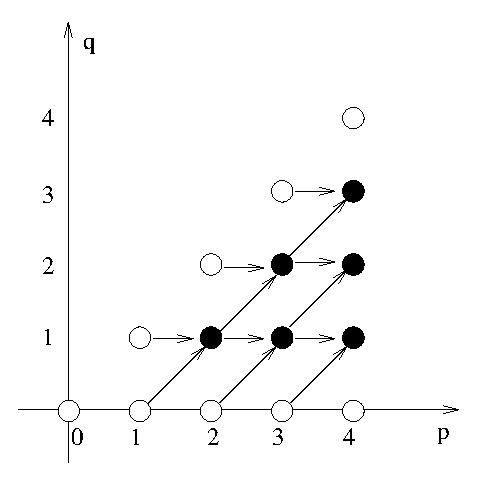
\includegraphics[width=1.5in]{indstep}
\par\end{centering}
\caption{Deriving Lemma~1 by induction. White circles correspond to the basis
of induction. Black circles are reached by induction steps.\label{fig:Deriving-Lemma-1}}
\end{figure}


\paragraph{Corollary:}

For any $\hat{A}\in\textrm{End }V$ and $\alpha\in\mathbb{K}$,
\[
\wedge^{p}(\hat{A}+\alpha\hat{1}_{V})^{q}=\sum_{r=0}^{q}\alpha^{q-r}{p-r \choose p-q}(\wedge^{p}\hat{A}^{r}).
\]


\subparagraph{Proof:}

By Statement~3 of Sec.~\ref{subsec:Extensions-of-an}, $\wedge^{p}(\alpha\hat{A})^{q}=\alpha^{q}(\wedge^{p}\hat{A}^{q})$.
Set $\hat{A}=\alpha\hat{B}$, where $\hat{B}$ is an auxiliary operator,
and compute
\begin{align*}
\wedge^{p}(\alpha\hat{B}+\alpha\hat{1}_{V})^{q} & =\alpha^{q}\wedge^{p}(\hat{B}+\hat{1}_{V})^{q}=\alpha^{q}\sum_{r=0}^{q}{p-r \choose p-q}(\wedge^{p}\hat{B}^{r})\\
 & =\sum_{r=0}^{q}\alpha^{q-r}{p-r \choose p-q}(\wedge^{p}(\alpha\hat{B})^{r})\\
 & =\sum_{r=0}^{q}\alpha^{q-r}{p-r \choose p-q}(\wedge^{p}\hat{A}^{r}).
\end{align*}
\hfill{}$\blacksquare$

\paragraph{Theorem 2:}

The coefficients $q_{m}(\hat{A})$, $1\leq m\leq N$ of the characteristic
polynomial, defined by 
\[
Q_{\hat{A}}\left(\lambda\right)=\left(-\lambda\right)^{N}+\sum_{k=0}^{N-1}\left(-1\right)^{k}q_{N-k}(\hat{A})\lambda^{k},
\]
are the numbers corresponding to the operators $\wedge^{N}\hat{A}^{m}\in\textrm{End}(\wedge^{N}V)$:
\[
q_{m}(\hat{A})\hat{1}_{\wedge^{N}V}=\wedge^{N}\hat{A}^{m}.
\]
In particular, $q_{N}(\hat{A})=\det\hat{A}$ and $q_{1}(\hat{A})=\textrm{Tr}\hat{A}$.
More compactly, the statement can be written as
\[
Q_{\hat{A}}\left(\lambda\right)\hat{1}_{\wedge^{N}V}=\sum_{k=0}^{N}\left(-\lambda\right)^{N-k}(\wedge^{N}\hat{A}^{k}).
\]


\subparagraph{Proof:}

This is now a consequence of Lemma~1 and its Corollary, where we
set $p=q=N$ and obtain
\[
\wedge^{N}(\hat{A}-\lambda\hat{1}_{V})^{N}=\sum_{r=0}^{N}\left(-\lambda\right)^{N-r}(\wedge^{N}\hat{A}^{r}).
\]
 \hfill{}$\blacksquare$

\paragraph{Exercise 1:}

\label{par:Trace relation1}Show that the characteristic polynomial
of an operator $\hat{A}$ in a \emph{three-dimen\-sion\-al} space
$V$ can be written as
\[
Q_{\hat{A}}(\lambda)=\det\hat{A}-{\textstyle \frac{1}{2}}\big[(\text{Tr}\hat{A})^{2}-\text{Tr}(\hat{A}^{2})\big]\lambda+(\text{Tr}\hat{A})\lambda^{2}-\lambda^{3}.
\]


\subparagraph{Solution:}

The first and the third coefficients of $Q_{\hat{A}}(\lambda)$ are,
as usual, the determinant and the trace of $\hat{A}$. The second
coefficient is equal to $-{\wedge^{3}\hat{A}^{2}}$, so we need to
show that
\[
\wedge^{3}\hat{A}^{2}=\frac{1}{2}\big[(\text{Tr}\hat{A})^{2}-\text{Tr}(\hat{A}^{2})\big].
\]
We apply the operator $\wedge^{3}\hat{A}^{1}$ twice to a tensor $\mathbf{a}\wedge\mathbf{b}\wedge\mathbf{c}$
and calculate:
\begin{align*}
 & (\text{Tr}\hat{A})^{2}\mathbf{a}\wedge\mathbf{b}\wedge\mathbf{c}=(\wedge^{3}\hat{A}^{1})(\wedge^{3}\hat{A}^{1})(\mathbf{a}\wedge\mathbf{b}\wedge\mathbf{c})\\
 & =(\wedge^{3}\hat{A}^{1})(\hat{A}\mathbf{a}\wedge\mathbf{b}\wedge\mathbf{c}+\mathbf{a}\wedge\hat{A}\mathbf{b}\wedge\mathbf{c}+\mathbf{a}\wedge\mathbf{b}\wedge\hat{A}\mathbf{c})\\
 & =\hat{A}^{2}\mathbf{a}\wedge\mathbf{b}\wedge\mathbf{c}+2\hat{A}\mathbf{a}\wedge\hat{A}\mathbf{b}\wedge\mathbf{c}+\mathbf{a}\wedge\hat{A}^{2}\mathbf{b}\wedge\mathbf{c}\\
 & +2\hat{A}\mathbf{a}\wedge\mathbf{b}\wedge\hat{A}\mathbf{c}+2\mathbf{a}\wedge\hat{A}\mathbf{b}\wedge\hat{A}\mathbf{c}+\mathbf{a}\wedge\mathbf{b}\wedge\hat{A}^{2}\mathbf{c}\\
 & =\big[\text{Tr}(\hat{A}^{2})+2\wedge^{3}\hat{A}^{2}\big]\mathbf{a}\wedge\mathbf{b}\wedge\mathbf{c}.
\end{align*}
Then the desired formula follows.\hfill{}$\blacksquare$

\paragraph{Exercise 2 (general trace relations):}

\index{trace relations}Generalize the result of Exercise~1 to $N$
dimensions:

a) Show that 
\[
\wedge^{N}\hat{A}^{2}={\textstyle \frac{1}{2}}\big[(\text{Tr}\hat{A})^{2}-\text{Tr}(\hat{A}^{2})\big].
\]

b){*} Show that all coefficients $\wedge^{N}\hat{A}^{k}$ ($k=1,...,N$)
can be expressed as polynomials in $\text{Tr}\hat{A}$, $\text{Tr}(\hat{A}^{2})$,
..., $\text{Tr}(\hat{A}^{N})$.

\emph{Hint}: Define a ``mixed'' operator $\wedge^{N}(\hat{A}^{n})^{j}\hat{A}^{k}$
as a sum of exterior products containing $j$ times $\hat{A}^{n}$
and $k$ times $\hat{A}$; for example,
\begin{align*}
 & \big[{\wedge^{3}(\hat{A}^{2})^{1}\hat{A}^{1}}\big]\mathbf{a}\wedge\mathbf{b}\wedge\mathbf{c}\equiv\hat{A}^{2}\mathbf{a}\wedge(\hat{A}\mathbf{b}\wedge\mathbf{c}+\mathbf{b}\wedge\hat{A}\mathbf{c})\\
 & +\hat{A}\mathbf{a}\wedge(\hat{A}^{2}\mathbf{b}\wedge\mathbf{c}+\mathbf{b}\wedge\hat{A}^{2}\mathbf{c})+\mathbf{a}\wedge(\hat{A}^{2}\mathbf{b}\wedge\hat{A}\mathbf{c}+\hat{A}\mathbf{b}\wedge\hat{A}^{2}\mathbf{c}).
\end{align*}
By applying several operators $\wedge^{N}\hat{A}^{k}$ and $\text{Tr}(\hat{A}^{k})$
to an exterior product, derive identities connecting these operators
and $\wedge^{N}\hat{A}^{k}$: 
\begin{align*}
(\wedge^{N}\hat{A}^{1})(\wedge^{N}\hat{A}^{k}) & =(k+1)\wedge^{N}\hat{A}^{k+1}+\wedge^{N}(\hat{A}^{2})^{1}\hat{A}^{k-1},\\
\text{Tr}(\hat{A}^{k})\text{Tr}(\hat{A}) & =\text{Tr}(\hat{A}^{k+1})+\wedge^{N}(\hat{A}^{k})^{1}\hat{A}^{1},
\end{align*}
for $k=2,...,N-1$. Using these identities, show by induction that
operators of the form $\wedge^{N}\hat{A}^{k}$ ($k=1,...,N$) can
be all expressed through $\text{Tr}\hat{A}$, $\text{Tr}(\hat{A}^{2})$,
..., $\text{Tr}(\hat{A}^{N-1})$ as polynomials. 

As an example, here is the trace relation for $\wedge^{N}\hat{A}^{3}$:
\[
\wedge^{N}\hat{A}^{3}={\textstyle \frac{1}{6}}(\text{Tr}\hat{A})^{3}-{\textstyle \frac{1}{2}}(\text{Tr}\hat{A})\text{Tr}(\hat{A}^{2})+{\textstyle \frac{1}{3}}\text{Tr}(\hat{A}^{3}).
\]
Note that in three dimensions this formula directly yields the determinant
of $\hat{A}$ expressed through traces of powers of $\hat{A}$. Below
(Sec.~\ref{subsec:General-trace-relations}) we will derive a formula
for the general trace relation.\hfill{}$\blacksquare$

Since operators in $\wedge^{N}V$ act as multiplication by a number,
it is convenient to omit $\hat{1}_{\wedge^{N}V}$ and regard expressions
such as $\wedge^{N}\hat{A}^{k}$ as simply numbers. More formally,
there is a canonical isomorphism between $\textrm{End}\left(\wedge^{N}V\right)$
and $\mathbb{K}$ (even though there is no canonical isomorphism between
$\wedge^{N}V$ and $\mathbb{K}$).

\paragraph{Exercise 3:}

Give an explicit formula for the canonical isomorphism: a) between
$\left(\wedge^{k}V\right)^{*}$ and $\wedge^{k}(V^{*})$; b) between
$\textrm{End}\left(\wedge^{N}V\right)$ and $\mathbb{K}$. 

\subparagraph{Answer:}

a) A tensor $\mathbf{f}_{1}^{*}\wedge...\wedge\mathbf{f}_{k}^{*}\in\wedge^{k}(V^{*})$
acts as a linear function on a tensor $\mathbf{v}_{1}\wedge...\wedge\mathbf{v}_{k}\in\wedge^{k}V$
by the formula
\[
\left(\mathbf{f}_{1}^{*}\wedge...\wedge\mathbf{f}_{k}^{*}\right)\left(\mathbf{v}_{1}\wedge...\wedge\mathbf{v}_{k}\right)\equiv\det(A_{jk}),
\]
where $A_{jk}$ is the square matrix defined by $A_{jk}\equiv\mathbf{f}_{j}^{*}(\mathbf{v}_{k})$.

b) Since $(\wedge^{N}V)^{*}$ is canonically isomorphic to $\wedge^{N}(V^{*})$,
an operator $\hat{N}\in\textrm{End}\left(\wedge^{N}V\right)$ can
be represented by a tensor 
\[
\hat{N}=\left(\mathbf{v}_{1}\wedge...\wedge\mathbf{v}_{N}\right)\otimes\left(\mathbf{f}_{1}^{*}\wedge...\wedge\mathbf{f}_{N}^{*}\right)\in\left(\wedge^{N}V\right)\otimes\left(\wedge^{N}V^{*}\right).
\]
The isomorphism maps $\hat{N}$ into the number $\det(A_{jk})$, where
$A_{jk}$ is the square matrix defined by $A_{jk}\equiv\mathbf{f}_{j}^{*}(\mathbf{v}_{k})$.\hfill{}$\blacksquare$

\paragraph{Exercise 4:}

Show that an operator $\hat{A}\in\textrm{End }V$ and its canonical
transpose operator $\hat{A}^{T}\in\textrm{End }V^{*}$ have the same
characteristic polynomials.

\emph{Hint}: Consider the operator $(\hat{A}-x\hat{1}_{V})^{T}$.\hfill{}$\blacksquare$

\paragraph{Exercise 5:}

Given an operator $\hat{A}$ of rank $r<N$, show that $\wedge^{N}\hat{A}^{k}=0$
for $k\geq r+1$ but $\wedge^{N}\hat{A}^{r}\neq0$.

\emph{Hint}: If $\hat{A}$ has rank $r<N$ then $\hat{A}\mathbf{v}_{1}\wedge...\wedge\hat{A}\mathbf{v}_{r+1}=0$
for any set of vectors $\left\{ \mathbf{v}_{1},...,\mathbf{v}_{r+1}\right\} $. 

\subsection{Nilpotent operators}

There are many operators with the same characteristic polynomial.
In particular, there are many operators which have the simplest possible
characteristic polynomial, $Q_{0}(x)=\left(-x\right)^{N}$. Note that
the zero operator has this characteristic polynomial. We will now
see how to describe all such operators $\hat{A}$ that $Q_{\hat{A}}(x)=\left(-x\right)^{N}$.

\paragraph{Definition:}

An operator $\hat{A}\in\textrm{End }V$ is \textbf{nilpotent}\index{nilpotent}
if there exists an integer $p\geq1$ such that $(\hat{A})^{p}=\hat{0}$,
where $\hat{0}$ is the zero operator and $(\hat{A})^{p}$ is the
$p$-th power of the operator $\hat{A}$.

\paragraph{Examples:}

a) The operator defined by the matrix $\left(\begin{array}{cc}
0 & \alpha\\
0 & 0
\end{array}\right)$ in some basis $\left\{ \mathbf{e}_{1},\mathbf{e}_{2}\right\} $ is
nilpotent for any number $\alpha$. This operator can be expressed
in tensor form as $\alpha\mathbf{e}_{1}\otimes\mathbf{e}_{2}^{*}$.

b) In the space of polynomials of degree at most $n$ in the variable
$x$, the linear operator $\frac{d}{dx}$ is nilpotent because the
$(n+1)$-th power of this operator will evaluate the $\left(n+1\right)$-th
derivative, which is zero on any polynomial of degree at most $n$.\hfill{}$\blacksquare$

\paragraph{Statement:}

If $\hat{A}$ is a nilpotent operator then $\hat{Q}_{\hat{A}}\left(x\right)=\left(-x\right)^{N}$.

\subparagraph{Proof:}

First an example: suppose that $N=2$ and that $\hat{A}^{3}=0$. By
Theorem~2, the coefficients of the characteristic polynomial of the
operator $\hat{A}$ correspond to the operators $\wedge^{N}\hat{A}^{k}$.
We need to show that all these operators are equal to zero.

Consider, for instance, $\wedge^{2}\hat{A}^{2}=q_{2}\hat{1}_{\wedge^{2}V}$.
This operator raised to the power $3$ acts on a tensor $\mathbf{a}\wedge\mathbf{b}\in\wedge^{2}V$
as
\[
{\big({\wedge^{2}\hat{A}^{2}}\big)}^{3}\mathbf{a}\wedge\mathbf{b}=\hat{A}^{3}\mathbf{a}\wedge\hat{A}^{3}\mathbf{b}=0
\]
since $\hat{A}^{3}=0$. On the other hand, 
\[
{\big({\wedge^{2}\hat{A}^{2}}\big)}^{3}\mathbf{a}\wedge\mathbf{b}=\left(q_{2}\right)^{3}\mathbf{a}\wedge\mathbf{b}.
\]
 Therefore $q_{2}=0$. Now consider $\wedge^{2}\hat{A}^{1}$ to the
power $3$,
\[
{\big({\wedge^{2}\hat{A}^{1}}\big)}^{3}\mathbf{a}\wedge\mathbf{b}=\hat{A}^{2}\mathbf{a}\wedge\hat{A}\mathbf{b}+\hat{A}\mathbf{a}\wedge\hat{A}^{2}\mathbf{b}
\]
(all other terms vanish because $\hat{A}^{3}=0$). It is clear that
the operator $\wedge^{2}\hat{A}^{1}$ to the power $6$ vanishes because
there will be at least a third power of $\hat{A}$ acting on each
vector. Therefore $q_{1}=0$ as well.

Now a general argument. Let $p$ be a positive integer such that $\hat{A}^{p}=0$,
and consider the $(pN)$-th power of the operator $\wedge^{N}\hat{A}^{k}$
for some $k\geq1$. We will prove that $(\wedge^{N}\hat{A}^{k})^{pN}=\hat{0}$.
Since $\wedge^{N}\hat{A}^{k}$ is a multiplication by a number, from
$(\wedge^{N}\hat{A}^{k})^{pN}=0$ it will follow that $\wedge^{N}\hat{A}^{k}$
is a zero operator in $\wedge^{N}V$ for all $k\geq1$. If all the
coefficients $q_{k}$ of the characteristic polynomial vanish, we
will have $Q_{\hat{A}}\left(x\right)=\left(-x\right)^{N}$.

To prove that $(\wedge^{N}\hat{A}^{k})^{pN}=\hat{0}$, consider the
action of the operator $(\wedge^{N}\hat{A}^{k})^{pN}$ on a tensor
$\mathbf{e}_{1}\wedge...\wedge\mathbf{e}_{N}\in\wedge^{N}V$. By definition
of $\wedge^{N}\hat{A}^{k}$, this operator is a sum of terms of the
form
\[
\hat{A}^{s_{1}}\mathbf{e}_{1}\wedge...\wedge\hat{A}^{s_{N}}\mathbf{e}_{N},
\]
where $s_{j}=0$ or $s_{j}=1$ are chosen such that $\sum_{j=1}^{N}s_{j}=k$.
Therefore, the same operator raised to the power $pN$ is expressed
as
\begin{equation}
(\wedge^{N}\hat{A}^{k})^{pN}=\sum_{(s_{1},...,s_{n})}\hat{A}^{s_{1}}\mathbf{e}_{1}\wedge...\wedge\hat{A}^{s_{N}}\mathbf{e}_{N},\label{eq:sum pN}
\end{equation}
where now $s_{j}$ are non-negative integers, $0\leq s_{j}\leq pN$,
such that $\sum_{j=1}^{N}s_{j}=kpN$. It is impossible that all $s_{j}$
in Eq.~(\ref{eq:sum pN}) are less than $p$, because then we would
have $\sum_{j=1}^{N}s_{j}<Np$, which would contradict the condition
$\sum_{j=1}^{N}s_{j}=kpN$ (since $k\geq1$ by construction). So each
term of the sum in Eq.~(\ref{eq:sum pN}) contains at least a $p$-th
power of $\hat{A}$. Since $(\hat{A})^{p}=0$, each term in the sum
in Eq.~(\ref{eq:sum pN}) vanishes. Hence $(\wedge^{N}\hat{A}^{k})^{pN}=0$
as required.\hfill{}$\blacksquare$

\paragraph{Remark:}

The converse statement is also true: If the characteristic polynomial
of an operator $\hat{A}$ is $Q_{\hat{A}}(x)=\left(-x\right)^{N}$
then $\hat{A}$ is nilpotent. This follows easily from the Cayley-Hamilton
theorem (see below), which states that $Q_{\hat{A}}(\hat{A})=0$,
so we obtain immediately $(\hat{A})^{N}=0$, i.e.~the operator $\hat{A}$
is nilpotent. We find that one cannot distinguish a nilpotent operator
from the zero operator by looking only at the characteristic polynomial.

\chapter{Advanced applications}

In this chapter we work in an $N$-dimen\-sion\-al vector space
over a number field $\mathbb{K}$. 

\section{The space $\wedge^{N-1}V$}

So far we have been using only the top exterior power, $\wedge^{N}V$.
The next-to-top exterior power space, $\wedge^{N-1}V$, has the same
dimension as $V$ and is therefore quite useful since it is a space,
in some special sense, associated with $V$. We will now find several
important uses of this space. 

\subsection{Exterior transposition of operators\label{subsec:The-next-to-top-exterior}}

We have seen that a linear operator in the space $\wedge^{N}V$ is
equivalent to multiplication by a number. We can reformulate this
statement by saying that the space of linear operators in $\wedge^{N}V$
is canonically isomorphic to $\mathbb{K}$. Similarly, the space of
linear operators in $\wedge^{N-1}V$ is canonically isomorphic to
$\text{End}\,V$, the space of linear operators in $V$. The isomorphism
map will be denoted by the superscript $^{\wedge T}$. We will begin
by defining this map explicitly.

\paragraph{Question:}

What is a nontrivial example of a linear operator in $\wedge^{N-1}V$?

\subparagraph{Answer:}

Any operator of the form $\wedge^{N-1}\hat{A}^{p}$ with $1\leq p\leq N-1$
and $\hat{A}\in\text{End}\,V$. In this book, operators constructed
in this way will be the only instance of operators in $\wedge^{N-1}V$. 

\paragraph{Definition:}

If $\hat{X}\in\textrm{End}\,V$ is a given linear operator then the
\textbf{exterior} \textbf{transpose}\index{exterior transposition}
operator
\[
\hat{X}^{\wedge T}\in\textrm{End}\left(\wedge^{N-1}V\right)
\]
 is canonically defined by the formula 
\[
\big(\hat{X}^{\wedge T}\omega\big)\wedge\mathbf{v}\equiv\omega\wedge\hat{X}\mathbf{v},
\]
which must hold for all $\omega\in\wedge^{N-1}V$ and all $\mathbf{v}\in V$.
If $\hat{Y}\in\text{End}(\wedge^{N-1}V)$ is a linear operator then
its exterior transpose $\hat{Y}^{\wedge T}\in\text{End}\,V$ is defined
by the formula
\[
\omega\wedge\big(\hat{Y}^{\wedge T}\mathbf{v}\big)\equiv(\hat{Y}\omega)\wedge\mathbf{v},\quad\forall\omega\in\wedge^{N-1}V,\;\mathbf{v}\in V.
\]

We need to check that the definition makes sense, i.e.~that the operators
defined by these formulas exist and are uniquely defined.

\paragraph{Statement 1:}

The exterior transpose operators are well-defined, i.e.~they exist,
are unique, and are linear operators in the respective spaces. The
exterior transposition has the linearity property
\[
(\hat{A}+\lambda\hat{B})^{\wedge T}=\hat{A}^{\wedge T}+\lambda\hat{B}^{\wedge T}.
\]
If $\hat{X}\in\textrm{End}\,V$ is an exterior transpose of $\hat{Y}\in\text{End}\left(\wedge^{N-1}V\right)$,
i.e.~$\hat{X}=\hat{Y}^{\wedge T}$, then also conversely $\hat{Y}=\hat{X}^{\wedge T}$.

\subparagraph{Proof:}

We need to show that the formula 
\[
\big(\hat{X}^{\wedge T}\omega\big)\wedge\mathbf{v}\equiv\omega\wedge\hat{X}\mathbf{v}
\]
actually defines an operator $\hat{X}^{\wedge T}$ uniquely when $\hat{X}\in\textrm{End}\,V$
is a given operator. Let us fix a tensor $\omega\in\wedge^{N-1}V$;
to find $\hat{X}^{\wedge T}\omega$ we need to determine a tensor
$\psi\in\wedge^{N-1}V$ such that $\psi\wedge\mathbf{v}=\omega\wedge\hat{X}\mathbf{v}$
for all $\mathbf{v}\in V$. When we find such a $\psi$, we will also
show that it is unique; then we will have shown that $\hat{X}^{\wedge T}\omega\equiv\psi$
is well-defined.

An explicit computation of the tensor $\psi$ can be performed in
terms of a basis $\left\{ \mathbf{e}_{1},...,\mathbf{e}_{N}\right\} $
in $V$. A basis in the space $\wedge^{N-1}V$ is formed by the set
of $N$ tensors of the form $\boldsymbol{\omega}_{i}\equiv\mathbf{e}_{1}\wedge...\wedge\mathbf{e}_{i-1}\wedge\mathbf{e}_{i+1}\wedge...\wedge\mathbf{e}_{N}$,
that is, $\boldsymbol{\omega}_{i}$ is the exterior product of the
basis vectors without the vector $\mathbf{e}_{i}$ ($1\leq i\leq N$).
In the notation of Sec.~\ref{subsec:Computing-the-dual}, we have
$\boldsymbol{\omega}_{i}=*(\mathbf{e}_{i})(-1)^{i-1}$. It is sufficient
to determine the components of $\psi$ in this basis,
\[
\psi=\sum_{i=1}^{N}c_{i}\boldsymbol{\omega}_{i}.
\]
 Taking the exterior product of $\psi$ with $\mathbf{e}_{i}$, we
find that only the term with $c_{i}$ survives,
\[
\psi\wedge\mathbf{e}_{i}=(-1)^{N-i}c_{i}\mathbf{e}_{1}\wedge...\wedge\mathbf{e}_{N}.
\]
Therefore, the coefficient $c_{i}$ is uniquely determined from the
condition 
\[
c_{i}\mathbf{e}_{1}\wedge...\wedge\mathbf{e}_{N}=(-1)^{N-i}\psi\wedge\mathbf{e}_{i}{\lyxbuildrel!\above=}(-1)^{N-i}\omega\wedge\hat{X}\mathbf{e}_{i}.
\]
Since the operator $\hat{X}$ is given, we know all $\hat{X}\mathbf{e}_{i}$
and can compute $\omega\wedge\hat{X}\mathbf{e}_{i}\in\wedge^{N}V$.
So we find that every coefficient $c_{i}$ is uniquely determined.

It is seen from the above formula that each coefficient $c_{i}$ depends
linearly on the operator $\hat{X}$. Therefore the linearity property
holds,
\[
(\hat{A}+\lambda\hat{B})^{\wedge T}=\hat{A}^{\wedge T}+\lambda\hat{B}^{\wedge T}.
\]

The linearity of the operator $\hat{X}^{\wedge T}$ follows straightforwardly
from the identity
\begin{align*}
\big(\hat{X}^{\wedge T}(\omega+\lambda\omega^{\prime})\big)\wedge\mathbf{v} & {\lyxbuildrel!\above=}\left(\omega+\lambda\omega^{\prime}\right)\wedge\hat{X}\mathbf{v}\\
 & =\omega\wedge\hat{X}\mathbf{v}+\lambda\omega^{\prime}\wedge\hat{X}\mathbf{v}\\
 & {\lyxbuildrel!\above=}(\hat{X}^{\wedge T}\omega)\wedge\mathbf{v}+\lambda(\hat{X}^{\wedge T}\omega^{\prime})\wedge\mathbf{v}.
\end{align*}
In the same way we prove the existence, the uniqueness, and the linearity
of the exterior transpose of an operator from $\text{End}(\wedge^{N-1}V)$.
It is then clear that the transpose of the transpose is again the
original operator. Details left as exercise.\hfill{}$\blacksquare$

\paragraph{Remark:}

Note that the space $\wedge^{N-1}V$ is has the same dimension as
$V$ but is \emph{not} canonically isomorphic to $V$. Rather, an
element $\psi\in\wedge^{N-1}V$ naturally acts by exterior multiplication
on a vector $\mathbf{v}\in V$ and yields a tensor from $\wedge^{N}V$,
i.e.~$\psi$ is a linear map $V\rightarrow\wedge^{N}V$, and we may
express this as $\wedge^{N-1}V\cong V^{*}\otimes\wedge^{N}V$. Nevertheless,
as we will now show, the exterior transpose map allows us to establish
that the space of linear operators in $\wedge^{N-1}V$ is canonically
isomorphic to the space of linear operators in $V$. We will use this
isomorphism extensively in the following sections. A formal statement
follows.

\paragraph{Statement~2:}

The spaces $\textrm{End}(\wedge^{N-1}V)$ and $\textrm{End}\,V$ are
canonically isomorphic. 

\subparagraph{Proof:}

The map $^{\wedge T}$ between these spaces is one-to-one since no
two different operators are mapped to the same operator. If two different
operators $\hat{A},\hat{B}$ had the same exterior transpose, we would
have $(\hat{A}-\hat{B})^{\wedge T}=0$ and yet $\hat{A}-\hat{B}\neq0$.
There exists at least one $\omega\in\wedge^{N-1}V$ and $\mathbf{v}\in V$
such that $\omega\wedge(\hat{A}-\hat{B})\mathbf{v}\neq0$, and then
\[
0=\big((\hat{A}-\hat{B})^{\wedge T}\omega\big)\wedge\mathbf{v}=\omega\wedge(\hat{A}-\hat{B})\mathbf{v}\neq0,
\]
which is a contradiction. The map $^{\wedge T}$ is linear (Statement~1).
Therefore, it is an isomorphism between the vector spaces $\textrm{End}\left(\wedge^{N-1}V\right)$
and $\textrm{End}\,V$.\hfill{}$\blacksquare$

A generalization of Statement~1 is the following.

\paragraph{Exercise 1: }

Show that the spaces $\textrm{End}(\wedge^{k}V)$ and $\textrm{End}(\wedge^{N-k}V)$
are canonically isomorphic ($1\leq k<N$). Specifically, if $\hat{X}\in\textrm{End}(\wedge^{k}V)$
then the linear operator $\hat{X}^{\wedge T}\in\textrm{End}(\wedge^{N-k}V)$
is uniquely defined by the formula 
\[
\big(\hat{X}^{\wedge T}\omega_{N-k}\big)\wedge\omega_{k}\equiv\omega_{N-k}\wedge\hat{X}\omega_{k},
\]
which must hold for arbitrary tensors $\omega_{k}\in\wedge^{k}V$,
$\omega_{N-k}\in\wedge^{N-k}V$.

\paragraph{Remark:}

It follows that the exterior transpose of $\wedge^{N}\hat{A}^{N}\in\text{End}\left(\wedge^{N}V\right)$
is mapped by the canonical isomorphism to an element of $\text{End}\,\mathbb{K}$,
that is, a multiplication by a number. This is precisely the map we
have been using in the previous section to define the determinant.
In this notation, we have
\[
\det\hat{A}\equiv\big({\wedge^{N}\hat{A}^{N}}{\big)}^{\wedge T}.
\]
Here we identify $\text{End}\,\mathbb{K}$ with $\mathbb{K}$.

\paragraph{Exercise 2:}

For any operators $\hat{A},\hat{B}\in\text{End}\left(\wedge^{k}V\right)$,
show that
\[
(\hat{A}\hat{B})^{\wedge T}=\hat{B}^{\wedge T}\hat{A}^{\wedge T}.
\]


\subsection{{*} Index notation\label{subsec:-Index-notation for exterior transposition}}

Let us see how the exterior transposition\index{exterior transposition!in index notation}
is expressed in the index notation. (Below we will not use the resulting
formulas.)

If an operator $\hat{A}\in\text{End}\,V$ is given in the index notation
by a matrix $A_{i}^{j}$, the exterior transpose $\hat{A}^{\wedge T}\in\text{End}\left(\wedge^{N-1}V\right)$
is represented by an array $B_{i_{1}...i_{N-1}}^{j_{1}...j_{N-1}}$,
which is totally antisymmetric with respect to its $N-1$ lower and
upper indices separately. The action of the operator $\hat{B}\equiv\hat{A}^{\wedge T}$
on a tensor $\psi\in\wedge^{N-1}V$ is written in the index notation
as
\[
\sum_{i_{s}}B_{i_{1}...i_{N-1}}^{j_{1}...j_{N-1}}\psi^{i_{1}...i_{N-1}}.
\]
(Here we did not introduce any combinatorial factors; the factor $\left(N-1\right)!$
will therefore appear at the end of the calculation.)

By definition of the exterior transpose, for any vector $\mathbf{v}\in V$
and for any $\psi\in\wedge^{N-1}V$ we must have
\[
(\hat{B}\psi)\wedge\mathbf{v}=\psi\wedge(\hat{A}\mathbf{v}).
\]
Using the index representation of the exterior product through the
projection operators $\hat{E}$ (see Sec.~\ref{subsec:Exterior-product-in-index}),
we represent the equation above in the the index notation as 
\begin{align*}
 & \sum_{i,i_{s},j_{s}}E_{j_{1}...j_{N-1}i}^{k_{1}...k_{N}}(B_{i_{1}...i_{N-1}}^{j_{1}...j_{N-1}}\psi^{i_{1}...i_{N-1}})v^{i}\\
 & \;=\sum_{j_{s},i,j}E_{j_{1}...j_{N-1}j}^{k_{1}...k_{N}}\psi^{j_{1}...j_{N-1}}(A_{i}^{j}v^{i}).
\end{align*}
We may simplify this to 
\begin{align*}
 & \sum_{i,i_{s},j_{s}}\varepsilon_{j_{1}...j_{N-1}i}(B_{i_{1}...i_{N-1}}^{j_{1}...j_{N-1}}\psi^{i_{1}...i_{N-1}})v^{i}\\
 & \;=\sum_{i_{s},i,j}\varepsilon_{i_{1}...i_{N-1}j}\psi^{i_{1}...i_{N-1}}(A_{i}^{j}v^{i}),
\end{align*}
because $E_{j_{1}...j_{N}}^{k_{1}...k_{N}}=\varepsilon_{j_{1}...j_{N}}\varepsilon^{k_{1}...k_{N}}$,
and we may cancel the common factor $\varepsilon^{k_{1}...k_{N}}$
whose indices are not being summed over. 

Since the equation above should hold for arbitrary $\psi^{i_{1}...i_{N-1}}$
and $v^{i}$, the equation with the corresponding \emph{free} indices
$i_{s}$ and $i$ should hold: 
\begin{equation}
\sum_{j_{s}}\varepsilon_{j_{1}...j_{N-1}i}B_{i_{1}...i_{N-1}}^{j_{1}...j_{N-1}}=\sum_{j}\varepsilon_{i_{1}...i_{N-1}j}A_{i}^{j}.\label{eq:B A connection}
\end{equation}
This equation can be solved for $B$ as follows. We note that the
$\varepsilon$ symbol in the left-hand side of Eq.~(\ref{eq:B A connection})
has one free index, $i$. Let us therefore multiply with an additional
$\varepsilon$ and sum over that index; this will yield the projection
operator $\hat{E}$ (see Sec.~\ref{subsec:Exterior-product-in-index}).
Namely, we multiply both sides of Eq.~(\ref{eq:B A connection})
with $\varepsilon^{k_{1}...k_{N-1}i}$ and sum over $i$:
\begin{align*}
\sum_{j,i}\varepsilon^{k_{1}...k_{N-1}i}\varepsilon_{i_{1}...i_{N-1}j}A_{i}^{j} & =\sum_{j_{s},i}\varepsilon^{k_{1}...k_{N-1}i}\varepsilon_{j_{1}...j_{N-1}i}B_{i_{1}...i_{N-1}}^{j_{1}...j_{N-1}}\\
 & =\sum_{j_{s}}E_{j_{1}...j_{N-1}}^{k_{1}...k_{N-1}}B_{i_{1}...i_{N-1}}^{j_{1}...j_{N-1}},
\end{align*}
where in the last line we used the definition~(\ref{eq:E tilda def})--(\ref{eq:E def})
of the operator $\hat{E}$. Now we note that the right-hand side is
the index representation of the product of the operators $\hat{E}$
and $\hat{B}$ (both operators act in $\wedge^{N-1}V$). The left-hand
side is also an operator in $\wedge^{N-1}V$; denoting this operator
for brevity by $\hat{X}$, we rewrite the equation as
\[
\hat{E}\hat{B}=\hat{X}\in\text{End}\left(\wedge^{N-1}V\right).
\]
Using the property 
\[
\hat{E}=(N-1)!\hat{1}_{\wedge^{N-1}V}
\]
(see Exercise in Sec.~\ref{subsec:Exterior-product-in-index}), we
may solve the equation $\hat{E}\hat{B}=\hat{X}$ for $\hat{B}$ as
\[
\hat{B}=\frac{1}{(N-1)!}\hat{X}.
\]
Hence, the components of $\hat{B}\equiv\hat{A}^{\wedge T}$ are expressed
as
\[
B_{i_{1}...i_{N-1}}^{k_{1}...k_{N-1}}=\frac{1}{(N-1)!}\sum_{j,i}\varepsilon^{k_{1}...k_{N-1}i}\varepsilon_{i_{1}...i_{N-1}j}A_{i}^{j}.
\]

An analogous formula holds for the exterior transpose of an operator
in $\wedge^{n}V$, for any $n=2,...,N$. I give the formula without
proof and illustrate it by an example.

\paragraph{Statement:}

If $\hat{A}\in\text{End}\left(\wedge^{n}V\right)$ is given by its
components $A_{i_{1}...i_{n}}^{j_{1}...j_{n}}$ then the components
of $\hat{A}^{\wedge T}$ are
\begin{align*}
 & \big(\hat{A}^{\wedge T}\big)_{l_{1}...l_{N-n}}^{k_{1}...k_{N-n}}\\
 & \;=\frac{1}{n!(N-n)!}\sum_{j_{s},i_{s}}\varepsilon^{k_{1}...k_{N-n}i_{1}...i_{n}}\varepsilon_{l_{1}...l_{N-n}j_{1}...j_{n}}A_{i_{1}...i_{n}}^{j_{1}...j_{n}}.
\end{align*}


\paragraph{Example:}

Consider the exterior transposition $\hat{A}^{\wedge T}$ of the identity
operator $\hat{A}\equiv\hat{1}_{\wedge^{2}V}$. The components of
the identity operator are given by
\[
A_{i_{1}i_{2}}^{j_{1}j_{2}}=\delta_{i_{1}}^{j_{1}}\delta_{i_{2}}^{j_{2}},
\]
so the components of $\hat{A}^{\wedge T}$ are
\begin{align*}
\big(\hat{A}^{\wedge T}\big)_{l_{1}...l_{N-2}}^{k_{1}...k_{N-2}} & =\frac{1}{2!(N-2)!}\sum_{j_{s},i_{s}}\varepsilon^{k_{1}...k_{N-2}i_{1}i_{2}}\varepsilon_{l_{1}...l_{N-2}j_{1}j_{2}}A_{i_{1}i_{2}}^{j_{1}j_{2}}\\
 & =\frac{1}{2!(N-2)!}\sum_{i_{1},i_{2}}\varepsilon^{k_{1}...k_{N-2}i_{1}i_{2}}\varepsilon_{l_{1}...l_{N-2}i_{1}i_{2}}.
\end{align*}
Let us check that this array of components is the same as that representing
the operator $\hat{1}_{\wedge^{N-2}V}$. We note that the expression
above is the same as
\[
\frac{1}{\left(N-2\right)!}E_{l_{1}...l_{N-2}}^{k_{1}...k_{N-2}},
\]
where the numbers $E_{l_{1}...l_{n}}^{k_{1}...k_{n}}$ are defined
by Eqs.~(\ref{eq:E tilda def})--(\ref{eq:E def}). Since the operator
$\hat{E}$ in $\wedge^{N-2}V$ is equal to $\left(N-2\right)!\hat{1}_{\wedge^{N-2}V}$,
we obtain that
\[
\hat{A}^{\wedge T}=\hat{1}_{\wedge^{N-2}V}
\]
as required.

\section{Algebraic complement (adjoint) and beyond}

In Sec.~\ref{subsec:The-determinant-def} we defined the determinant
and derived various useful properties by considering, essentially,
the exterior transpose of ${\wedge^{N}\hat{A}^{p}}$ with $1\leq p\leq N$
(although we did not introduce this terminology back then). We have
just seen that the exterior transposition can be defined more generally
--- as a map from $\text{End}(\wedge^{k}V)$ to $\text{End}(\wedge^{N-k}V)$.
We will see in this section that the exterior transposition of the
operators ${\wedge^{N-1}\hat{A}^{p}}$ with $1\leq p\leq N-1$ yields
operators acting in $V$ that are quite useful as well.

\subsection{Definition of algebraic complement\label{subsec:The-algebraic-complement}}

While we proved that operators like $(\wedge^{N-1}\hat{A}^{p})^{\wedge T}$
are well-defined, we still have not obtained any explicit formulas
for these operators. We will now compute these operators explicitly
because they play an important role in the further development of
the theory. It will turn out that every operator of the form $(\wedge^{N-1}\hat{A}^{p})^{\wedge T}$
is a \emph{polynomial} in $\hat{A}$ with coefficients that are known
if we know the characteristic polynomial of $\hat{A}$. 

\paragraph{Example 1:}

Let us compute $(\wedge^{N-1}\hat{A}^{1})^{\wedge T}$. We consider,
as a first example, a three-dimen\-sion\-al ($N=3$) vector space
$V$ and a linear operator $\hat{A}\in\text{End}\,V$. We are interested
in the operator $(\wedge^{2}\hat{A}^{1})^{\wedge T}$. By definition
of the exterior transpose, 
\begin{align*}
\mathbf{a}\wedge\mathbf{b}\wedge(\wedge^{2}\hat{A}^{1})^{\wedge T}\mathbf{c} & =\big((\wedge^{2}\hat{A}^{1})(\mathbf{a}\wedge\mathbf{b})\big)\wedge\mathbf{c}\\
 & =\hat{A}\mathbf{a}\wedge\mathbf{b}\wedge\mathbf{c}+\mathbf{a}\wedge\hat{A}\mathbf{b}\wedge\mathbf{c}.
\end{align*}
We recognize a fragment of the operator $\wedge^{3}\hat{A}^{1}$ and
write 
\begin{align*}
(\wedge^{3}\hat{A}^{1})(\mathbf{a}\wedge\mathbf{b}\wedge\mathbf{c}) & =\hat{A}\mathbf{a}\wedge\mathbf{b}\wedge\mathbf{c}+\mathbf{a}\wedge\hat{A}\mathbf{b}\wedge\mathbf{c}+\mathbf{a}\wedge\mathbf{b}\wedge\hat{A}\mathbf{c}\\
 & =(\text{Tr}\,\hat{A})\mathbf{a}\wedge\mathbf{b}\wedge\mathbf{c},
\end{align*}
since this operator acts as multiplication by the trace of $\hat{A}$
(Section~\ref{subsec:The-trace}). It follows that
\begin{align*}
\mathbf{a}\wedge\mathbf{b}\wedge(\wedge^{2}\hat{A}^{1})^{\wedge T}\mathbf{c} & =(\text{Tr}\,\hat{A})\mathbf{a}\wedge\mathbf{b}\wedge\mathbf{c}-\mathbf{a}\wedge\mathbf{b}\wedge\hat{A}\mathbf{c}\\
 & =\mathbf{a}\wedge\mathbf{b}\wedge\big((\text{Tr}\,\hat{A})\mathbf{c}-\hat{A}\mathbf{c}\big).
\end{align*}
Since this must hold for arbitrary $\mathbf{a},\mathbf{b},\mathbf{c}\in V$,
it follows that
\[
(\wedge^{2}\hat{A}^{1})^{\wedge T}=(\text{Tr}\,\hat{A})\hat{1}_{V}-\hat{A}.
\]
Thus we have computed the operator $(\wedge^{2}\hat{A}^{1})^{\wedge T}$
in terms of $\hat{A}$ and the trace of $\hat{A}$. 

\paragraph{Example 2:}

Let us now consider the operator $(\wedge^{2}\hat{A}^{2})^{\wedge T}$.
We have
\[
\mathbf{a}\wedge\mathbf{b}\wedge(\wedge^{2}\hat{A}^{2})^{\wedge T}\mathbf{c}=\big((\wedge^{2}\hat{A}^{2})(\mathbf{a}\wedge\mathbf{b})\big)\wedge\mathbf{c}=\hat{A}\mathbf{a}\wedge\hat{A}\mathbf{b}\wedge\mathbf{c}.
\]
We recognize a fragment of the operator $\wedge^{3}\hat{A}^{2}$ and
write 
\[
(\wedge^{3}\hat{A}^{2})(\mathbf{a}\wedge\mathbf{b}\wedge\mathbf{c})=\hat{A}\mathbf{a}\wedge\hat{A}\mathbf{b}\wedge\mathbf{c}+\mathbf{a}\wedge\hat{A}\mathbf{b}\wedge\hat{A}\mathbf{c}+\hat{A}\mathbf{a}\wedge\mathbf{b}\wedge\hat{A}\mathbf{c}.
\]
Therefore,
\begin{align*}
\mathbf{a}\wedge\mathbf{b}\wedge(\wedge^{2}\hat{A}^{2})^{\wedge T}\mathbf{c} & =(\wedge^{3}\hat{A}^{2})(\mathbf{a}\wedge\mathbf{b}\wedge\mathbf{c})\\
 & -(\mathbf{a}\wedge\hat{A}\mathbf{b}+\hat{A}\mathbf{a}\wedge\mathbf{b})\wedge\hat{A}\mathbf{c}\\
^{(1)}=(\wedge^{3}\hat{A}^{2})(\mathbf{a}\wedge\mathbf{b}\wedge\mathbf{c}) & -\mathbf{a}\wedge\mathbf{b}\wedge(\wedge^{2}\hat{A}^{1})^{\wedge T}\hat{A}\mathbf{c}\\
=\mathbf{a}\wedge\mathbf{b}\wedge & \big({\wedge^{3}\hat{A}^{2}}-(\wedge^{2}\hat{A}^{1})^{\wedge T}\hat{A}\big)\mathbf{c},
\end{align*}
where $^{(1)}$ used the definition of the operator $(\wedge^{2}\hat{A}^{1})^{\wedge T}$.
It follows that 
\begin{align*}
(\wedge^{2}\hat{A}^{2})^{\wedge T} & =(\wedge^{3}\hat{A}^{2})\hat{1}_{V}-(\wedge^{2}\hat{A}^{1})^{\wedge T}\hat{A}\\
 & =(\wedge^{3}\hat{A}^{2})\hat{1}_{V}-(\text{Tr}\,\hat{A})\hat{A}+\hat{A}\hat{A}.
\end{align*}
Thus we have expressed the operator $(\wedge^{2}\hat{A}^{2})^{\wedge T}$
as a \emph{polynomial} \emph{in} $\hat{A}$. Note that $\wedge^{3}\hat{A}^{2}$
is the second coefficient of the characteristic polynomial of $\hat{A}$.

\paragraph{Exercise~1:}

Consider a three-dimen\-sion\-al space $V$, a linear operator $\hat{A}$,
and show that
\[
(\wedge^{2}\hat{A}^{2})^{\wedge T}\hat{A}\mathbf{v}=(\det\hat{A})\mathbf{v},\quad\forall\mathbf{v}\in V.
\]

\emph{Hint}: Consider $\mathbf{a}\wedge\mathbf{b}\wedge(\wedge^{2}\hat{A}^{2})^{\wedge T}\hat{A}\mathbf{c}=\hat{A}\mathbf{a}\wedge\hat{A}\mathbf{b}\wedge\hat{A}\mathbf{c}$.\hfill{}$\blacksquare$

These examples are straightforwardly generalized. We will now express
every operator of the form $(\wedge^{N-1}\hat{A}^{p})^{\wedge T}$
as a polynomial in $\hat{A}$. For brevity, we introduce the notation
\[
\hat{A}_{(k)}\equiv(\wedge^{N-1}\hat{A}^{N-k})^{\wedge T},\quad1\leq k\leq N-1.
\]


\paragraph{Lemma~1:}

For any operator $\hat{A}\in\textrm{End }V$ and for an integer $p$,
$1\leq p\leq N$, the following formula holds as an identity of operators
in $V$:
\[
{\big({\wedge^{N-1}\hat{A}^{p-1}}\big)}^{\wedge T}\hat{A}+{\big({\wedge^{N-1}\hat{A}^{p}}\big)}^{\wedge T}=(\wedge^{N}\hat{A}^{p})\hat{1}_{V}.
\]
Here, in order to provide a meaning for this formula in cases $p=1$
and $p=N$, we define $\wedge^{N-1}\hat{A}^{N}\equiv\hat{0}$ and
$\wedge^{N-1}\hat{A}^{0}\equiv\hat{1}$. In the shorter notation,
this is
\[
\hat{A}_{(k)}\hat{A}+\hat{A}_{(k-1)}=(\wedge^{N}\hat{A}^{N-k+1})\hat{1}_{V}.
\]
Note that $\wedge^{N}\hat{A}^{N-k+1}\equiv q_{k-1}$, where $q_{j}$
are the coefficients of the characteristic polynomial of $\hat{A}$
(see Sec.~\ref{subsec:The-characteristic-polynomial}).

\subparagraph{Proof:}

We use Statement~4 in Sec.~\ref{subsec:Extensions-of-an} with $\omega\equiv\mathbf{v}_{1}\wedge...\wedge\mathbf{v}_{N-1}$,
$m\equiv N-1$ and $k\equiv p$:
\[
\bigl(\wedge^{N-1}\hat{A}^{p}\omega\bigr)\wedge\mathbf{u}+\bigl(\wedge^{N-1}\hat{A}^{p-1}\omega\bigr)\wedge(\hat{A}\mathbf{u})=\wedge^{N}\hat{A}^{p}\left(\omega\wedge\mathbf{u}\right).
\]
This holds for $1\leq p\leq N-1$. Applying the definition of the
exterior transpose, we find
\[
\omega\wedge\bigl(\wedge^{N-1}\hat{A}^{p}{\bigr)}^{\wedge T}\mathbf{u}+\omega\wedge\bigl(\wedge^{N-1}\hat{A}^{p-1}{\bigr)}^{\wedge T}\hat{A}\mathbf{u}=(\wedge^{N}\hat{A}^{p})\omega\wedge\mathbf{u}.
\]
Since this holds for all $\omega\in\wedge^{N-1}V$ and $\mathbf{u}\in V$,
we obtain the required formula,
\[
\bigl(\wedge^{N-1}\hat{A}^{p}\bigr)^{\wedge T}+\omega\wedge\bigl(\wedge^{N-1}\hat{A}^{p-1}\bigr)^{\wedge T}\hat{A}=(\wedge^{N}\hat{A}^{p})\hat{1}_{V}.
\]
It remains to verify the case $p=N$. In that case we compute directly,
\begin{align*}
\bigl(\wedge^{N-1}\hat{A}^{N-1}\omega\bigr)\wedge(\hat{A}\mathbf{u}) & =\hat{A}\mathbf{v}_{1}\wedge...\wedge\hat{A}\mathbf{v}_{N-1}\wedge\hat{A}\mathbf{u}\\
 & =\wedge^{N}\hat{A}^{N}\left(\omega\wedge\mathbf{u}\right).
\end{align*}
Hence, 
\[
\big({\wedge^{N-1}\hat{A}^{N-1}}\big)^{\wedge T}\hat{A}=(\wedge^{N}\hat{A}^{N})\hat{1}_{V}\equiv(\det\hat{A})\hat{1}_{V}.
\]
\hfill{}$\blacksquare$

\paragraph{Remark:}

In these formulas we interpret the operators $\wedge^{N}\hat{A}^{p}\in\text{End}\left(\wedge^{N}V\right)$
as simply numbers multiplying some operators. This is justified since
$\wedge^{N}V$ is one-dimen\-sion\-al, and linear operators in it
act as multiplication by numbers. In other words, we implicitly use
the canonical isomorphism $\text{End}\left(\wedge^{N}V\right)\cong\mathbb{K}$.\hfill{}$\blacksquare$

\paragraph{Exercise 2:}

Use induction in $p$ (for $1\leq p\leq N-1$) and Lemma~1 to express
$\hat{A}_{(k)}$ explicitly as polynomials in $\hat{A}$: 
\[
\hat{A}_{(N-p)}\equiv{\big({\wedge^{N-1}\hat{A}^{p}}\big)}^{\wedge T}=\sum_{k=0}^{p}\left(-1\right)^{k}(\wedge^{N}\hat{A}^{p-k}){(\hat{A})}^{k}.
\]
\emph{Hint}: Start applying Lemma~1 with $p=1$ and $\hat{A}_{(N)}\equiv\hat{1}$.\hfill{}$\blacksquare$

Using the coefficients $q_{k}\equiv\wedge^{N}\hat{A}^{N-k}$ of the
characteristic polynomial, the result of Exercise~2 can be rewritten
as
\begin{align*}
{\big({\wedge^{N-1}\hat{A}^{1}}\big)}^{\wedge T}\equiv\hat{A}_{(N-1)} & =q_{N-1}\hat{1}_{V}-\hat{A},\\
{\big({\wedge^{N-1}\hat{A}^{2}}\big)}^{\wedge T}\equiv\hat{A}_{(N-2)} & =q_{N-2}\hat{1}_{V}-q_{N-1}\hat{A}+(\hat{A})^{2},\\
... & ...,\\
{\big({\wedge^{N-1}\hat{A}^{N-1}}\big)}^{\wedge T}\equiv\hat{A}_{(1)} & =q_{1}\hat{1}_{V}+q_{2}(-\hat{A})+...\\
 & +q_{N-1}(-\hat{A})^{N-2}+(-\hat{A})^{N-1}.
\end{align*}
Note that the characteristic polynomial of $\hat{A}$ is 
\[
Q_{\hat{A}}(\lambda)=q_{0}+q_{1}(-\lambda)+...+q_{N-1}{(-\lambda)}^{N-1}+(-\lambda)^{N}.
\]
Thus the operators denoted by $\hat{A}_{(k)}$ are computed as suitable
``fragments''' of the characteristic polynomial into which $\hat{A}$
is substituted instead of $\lambda$.

\paragraph{Exercise 3:{*}}

Using the definition of exterior transpose for general exterior powers
(Exercise~1 in Sec.~\ref{subsec:The-next-to-top-exterior}), show
that for $1\leq k\leq N-1$ and $1\leq p\leq k$ the following identity
holds, 
\[
\sum_{q=0}^{p}{\big({\wedge^{N-k}\hat{A}^{p-q}}\big)}^{\wedge T}(\wedge^{k}\hat{A}^{q})=(\wedge^{N}\hat{A}^{p})\hat{1}_{\wedge^{k}V}.
\]
Deduce that the operators ${\big({\wedge^{N-k}\hat{A}^{p}}\big)}^{\wedge T}$
can be expressed as polynomials in the (mutually commuting) operators
$\wedge^{k}\hat{A}^{j}$ ($1\leq j\leq k$).

\emph{Hint}s: Follow the proof of Statement~4 in Sec.~\ref{subsec:Extensions-of-an}.
The idea is to apply both sides to $\omega_{k}\wedge\omega_{N-k}$,
where $\omega_{k}\equiv\mathbf{v}_{1}\wedge...\wedge\mathbf{v}_{k}$
and $\omega_{N-k}=\mathbf{v}_{N-k+1}\wedge...\wedge\mathbf{v}_{N}$.
Since $\wedge^{N}\hat{A}^{p}$ acts on $\omega_{k}\wedge\omega_{N-k}$
by distributing $p$ copies of $\hat{A}$ among the $N$ vectors $\mathbf{v}_{j}$,
one needs to show that the same terms will occur when one first distributes
$q$ copies of $\hat{A}$ among the first $k$ vectors and $p-q$
copies of $\hat{A}$ among the last $N-k$ vectors, and then sums
over all $q$ from $0$ to $p$. Once the identity is proved, one
can use induction to express the operators ${\big({\wedge^{N-k}\hat{A}^{p}}\big)}^{\wedge T}$.
For instance, the identity with $k=2$ and $p=1$ yields
\[
{\big({\wedge^{N-2}\hat{A}^{0}}\big)}^{\wedge T}(\wedge^{2}\hat{A}^{1})+{\big({\wedge^{N-2}\hat{A}^{1}}\big)}^{\wedge T}(\wedge^{2}\hat{A}^{0})=(\wedge^{N}\hat{A}^{1})\hat{1}_{\wedge^{k}V}.
\]
Therefore
\[
{\big({\wedge^{N-2}\hat{A}^{1}}\big)}^{\wedge T}=(\text{Tr}\hat{A})\hat{1}_{\wedge^{k}V}-\wedge^{2}\hat{A}^{1}.
\]
Similarly, with $k=2$ and $p=2$ we find
\begin{align*}
{\big({\wedge^{N-2}\hat{A}^{2}}\big)}^{\wedge T}\negmedspace & =(\wedge^{N}\hat{A}^{2})\hat{1}_{\wedge^{k}V}-{\big({\wedge^{N-2}\hat{A}^{1}}\big)}^{\wedge T}(\wedge^{2}\hat{A}^{1})-\wedge^{2}\hat{A}^{2}\\
 & =(\wedge^{N}\hat{A}^{2})\hat{1}_{\wedge^{k}V}-(\text{Tr}\hat{A})(\wedge^{2}\hat{A}^{1})+(\wedge^{2}\hat{A}^{1})^{2}-\wedge^{2}\hat{A}^{2}.
\end{align*}
It follows by induction that all the operators ${\big({\wedge^{N-k}\hat{A}^{p}}\big)}^{\wedge T}$
are expressed as polynomials in $\wedge^{k}\hat{A}^{j}$.\hfill{}$\blacksquare$

At the end of the proof of Lemma~1 we have obtained a curious relation,
\[
\big({\wedge^{N-1}\hat{A}^{N-1}}\big)^{\wedge T}\hat{A}=(\det\hat{A})\hat{1}_{V}.
\]
If $\det\hat{A}\neq0$, we may divide by it and immediately find the
following result.

\paragraph{Lemma~2: }

If $\det\hat{A}\neq0$, the inverse operator satisfies 
\[
\hat{A}^{-1}=\frac{1}{\det\hat{A}}\big({\wedge^{N-1}\hat{A}^{N-1}}\big)^{\wedge T}.
\]

Thus we are able to express the inverse operator $\hat{A}^{-1}$ as
a \emph{polynomial} in $\hat{A}$. If $\det\hat{A}=0$ then the operator
$\hat{A}$ has no inverse, but the operator $\big({\wedge^{N-1}\hat{A}^{N-1}}\big)^{\wedge T}$
is still well-defined and sufficiently useful to deserve a special
name.

\paragraph{Definition:}

The \textbf{algebraic complement\index{algebraic complement}} (also
called the \textbf{adjoint}\index{adjoint}) of $\hat{A}$ is the
operator
\[
\tilde{\hat{A}}\equiv{\big({\wedge^{N-1}\hat{A}^{N-1}}\big)}^{\wedge T}\in\text{End}\,V.
\]


\paragraph{Exercise 4:}

Compute the algebraic complement of the operator $\hat{A}=\mathbf{a}\otimes\mathbf{b}^{*}$,
where $\mathbf{a}\in V$ and $\mathbf{b}\in V^{*}$, and $V$ is an
$N$-dimen\-sion\-al space ($N\geq2$). 

\subparagraph{Answer: }

Zero if $N\geq3$. For $N=2$ we use Example~1 to compute 
\[
(\wedge^{1}\hat{A}^{1})^{\wedge T}=(\text{Tr}\,\hat{A})\hat{1}-\hat{A}=\mathbf{b}^{*}(\mathbf{a})\hat{1}-\mathbf{a}\otimes\mathbf{b}^{*}.
\]


\paragraph{Exercise 5:}

For the operator $\hat{A}=\mathbf{a}\otimes\mathbf{b}^{*}$ in $N$-dimen\-sion\-al
space, as in Exercise~4, show that $\big({\wedge^{N-1}\hat{A}^{p}}\big)^{\wedge T}=0$
for $p\geq2$.

\subsection{Algebraic complement of a matrix}

The algebraic complement is usually introduced in terms of matrix
determinants. Namely, one takes a matrix $A_{ij}$ and deletes the
column number $k$ and the row number $l$. Then one computes the
determinant of the resulting matrix and multiplies by $(-1)^{k+l}$.
The result is the element $B_{kl}$ of the matrix that is the algebraic
complement of $A_{ij}$. I will now show that our definition is equivalent
to this one, if we interpret matrices as coefficients of linear operators
in a basis.

\paragraph{Statement:}

Let $\hat{A}\in\text{End}\,V$ and let $\left\{ \mathbf{e}_{j}\right\} $
be a basis in $V$. Let $A_{ij}$ be the matrix of the operator $\hat{A}$
in this basis. Let $\hat{B}=\big({\wedge^{N-1}\hat{A}^{N-1}}\big)^{\wedge T}$
and let $B_{kl}$ be the matrix of $\hat{B}$ in the same basis. Then
$B_{kl}$ is equal to $\left(-1\right)^{k+l}$ times the determinant
of the matrix obtained from $A_{ij}$ by deleting the column number
$k$ and the row number $l$.

\subparagraph{Proof:}

Given an operator $\hat{B}$, the matrix element $B_{kl}$ in the
basis $\left\{ \mathbf{e}_{j}\right\} $ can be computed as the coefficient
in the following relation (see Sec.~\ref{subsec:Computing-the-dual}),
\[
B_{kl}\mathbf{e}_{1}\wedge...\wedge\mathbf{e}_{N}=\mathbf{e}_{1}\wedge...\wedge\mathbf{e}_{k-1}\wedge(\hat{B}\mathbf{e}_{l})\wedge\mathbf{e}_{k+1}\wedge...\wedge\mathbf{e}_{N}.
\]
 Since $\hat{B}=\big({\wedge^{N-1}\hat{A}^{N-1}}\big)^{\wedge T}$,
we have
\[
B_{kl}\mathbf{e}_{1}\wedge...\wedge\mathbf{e}_{N}=\hat{A}\mathbf{e}_{1}\wedge...\wedge\hat{A}\mathbf{e}_{k-1}\wedge\mathbf{e}_{l}\wedge\hat{A}\mathbf{e}_{k+1}\wedge...\wedge\hat{A}\mathbf{e}_{N}.
\]
Now the right side can be expressed as the determinant of another
operator, call it $\hat{X}$,
\begin{align*}
B_{kl}\mathbf{e}_{1}\wedge...\wedge\mathbf{e}_{N} & =(\det\hat{X})\mathbf{e}_{1}\wedge...\wedge\mathbf{e}_{N}\\
=\hat{X}\mathbf{e}_{1}\wedge & ...\wedge\hat{X}\mathbf{e}_{k-1}\wedge\hat{X}\mathbf{e}_{k}\wedge\hat{X}\mathbf{e}_{k+1}\wedge...\wedge\hat{X}\mathbf{e}_{N},
\end{align*}
if we define $\hat{X}$ as an operator such that $\hat{X}\mathbf{e}_{k}\equiv\mathbf{e}_{l}$
while on other basis vectors $\hat{X}\mathbf{e}_{j}\equiv\hat{A}\mathbf{e}_{j}$
($j\neq k$). Having defined $\hat{X}$ in this way, we have $B_{kl}=\det\hat{X}$. 

We can now determine the matrix $X_{ij}$ representing $\hat{X}$
in the basis $\left\{ \mathbf{e}_{j}\right\} $. By the definition
of the matrix representation of operators,
\[
\hat{A}\mathbf{e}_{j}=\sum_{i=1}^{N}A_{ij}\mathbf{e}_{i},\quad\hat{X}\mathbf{e}_{j}=\sum_{i=1}^{N}X_{ij}\mathbf{e}_{i},\quad1\leq j\leq N.
\]
It follows that $X_{ij}=A_{ij}$ for $j\neq k$ while $X_{ik}=\delta_{il}$
($1\leq i\leq N$), which means that the entire $k$-th column in
the matrix $A_{ij}$ has been replaced by a column containing zeros
except for a single nonzero element $X_{lk}=1$. 

It remains to show that the determinant of the matrix $X_{ij}$ is
equal to $\left(-1\right)^{k+l}$ times the determinant of the matrix
obtained from $A_{ij}$ by deleting column $k$ and row $l$. We may
move in the matrix $X_{ij}$ the $k$-th column to the first column
and the $l$-th row to the first row, without changing the order of
any other rows and columns. This produces the sign factor $\left(-1\right)^{k+l}$
but otherwise does not change the determinant. The result is
\begin{align*}
B_{kl} & =\det\hat{X}=\left(-1\right)^{k+l}\det\left|\begin{array}{cccc}
1 & X_{12} & ... & X_{1N}\\
0 & * & * & *\\
\vdots & * & * & *\\
0 & * & * & *
\end{array}\right|\\
 & =\left(-1\right)^{k+l}\det\left|\begin{array}{ccc}
* & * & *\\
* & * & *\\
* & * & *
\end{array}\right|,
\end{align*}
where the stars represent the matrix obtained from $A_{ij}$ by deleting
column $k$ and row $l$, and the numbers $X_{12}$, ..., $X_{1N}$
do not enter the determinant. This is the result we needed.\hfill{}$\blacksquare$

\paragraph{Exercise 5:{*}}

Show that the matrix representation of the algebraic complement can
be written through the Levi-Civita symbol\index{Levi-Civita symbol}
$\varepsilon$ as 
\[
\tilde{A}_{k}^{i}=\frac{1}{(N-1)!}\sum_{i_{2},...,i_{N}}\sum_{k_{2},...,k_{N}}\varepsilon_{kk_{2}...k_{N}}\varepsilon^{ii_{2}...i_{N}}A_{i_{2}}^{k_{2}}...A_{i_{N}}^{k_{N}}.
\]
\emph{Hint}: See Sections~\ref{subsec:Index-notation-for-determinants}
and \ref{subsec:-Index-notation for exterior transposition}.

\subsection{Further properties and generalizations\label{subsec:Properties-of-the-algebraic-complement}}

In our approach, the algebraic complement $\tilde{\hat{A}}$ of an
operator $\hat{A}$ comes from considering the set of $N-1$ operators
\[
\hat{A}_{(k)}\equiv\big({\wedge^{N-1}\hat{A}^{N-k}}\big)^{\wedge T},\quad1\leq k\leq N-1.
\]
(For convenience we might define $\hat{A}_{(N)}\equiv\hat{1}_{V}$.) 

The operators  $\hat{A}_{(k)}$ can be expressed as polynomials in
$\hat{A}$ through the identity (Lemma~1 in Sec.~\ref{subsec:The-algebraic-complement})
\[
\hat{A}_{(k)}\hat{A}+\hat{A}_{(k-1)}=q_{k-1}\hat{1},\quad q_{j}\equiv\wedge^{N}\hat{A}^{N-j}.
\]
The numbers $q_{j}$ introduced here are the coefficients of the characteristic
polynomial of $\hat{A}$; for instance, $\det\hat{A}\equiv q_{0}$
and $\text{Tr}\hat{A}\equiv q_{N-1}$. It follows by induction (Exercise~2
in Sec.~\ref{subsec:The-algebraic-complement}) that
\begin{align*}
\hat{A}_{(N-k)} & =q_{N-k}\hat{1}-q_{N-k+1}\hat{A}+...\\
 & \quad+q_{N-1}(-\hat{A})^{k-1}+(-\hat{A})^{k}.
\end{align*}
The algebraic complement is $\tilde{\hat{A}}\equiv\hat{A}_{1}$, but
it appears natural to study the properties of all the operators $\hat{A}_{(k)}$.
(The operators $\hat{A}_{(k)}$ do not seem to have an established
name for $k\geq2$.)

\paragraph{Statement~1:}

The coefficients of the characteristic polynomial of the algebraic
complement, $\tilde{\hat{A}}$, are
\[
\wedge^{N}\tilde{\hat{A}}^{k}=(\det\hat{A})^{k-1}(\wedge^{N}\hat{A}^{N-k})\equiv q_{0}^{k-1}q_{k}.
\]
For instance, 
\begin{align*}
\text{Tr}\,\tilde{\hat{A}} & =\wedge^{N}\tilde{\hat{A}}^{1}=q_{1}=\wedge^{N}\hat{A}^{N-1},\\
\det\tilde{\hat{A}} & =\wedge^{N}\tilde{\hat{A}}^{N}=q_{0}^{N-1}q_{N}=(\det\hat{A})^{N-1}.
\end{align*}


\subparagraph{Proof:}

Let us first assume that $\det\hat{A}\equiv q_{0}\neq0$. We use the
property $\hat{A}\tilde{\hat{A}}=q_{0}\hat{1}$ (Lemma~2 in Sec.~\ref{subsec:The-algebraic-complement})
and the multiplicativity of determinants to find
\begin{align*}
\det(\tilde{\hat{A}}-\lambda\hat{1})q_{0} & =\det(q_{0}\hat{1}-\lambda\hat{A})=(-\lambda)^{N}\det(\hat{A}-\frac{q_{0}}{\lambda}\hat{1})\\
 & =(-\lambda^{N})Q_{\hat{A}}(\frac{q_{0}}{\lambda}),
\end{align*}
hence the characteristic polynomial of $\tilde{\hat{A}}$ is 
\begin{align*}
Q_{\tilde{\hat{A}}}(\lambda) & \equiv\det(\tilde{\hat{A}}-\lambda\hat{1})=\frac{(-\lambda^{N})}{q_{0}}Q_{\hat{A}}(\frac{q_{0}}{\lambda})\\
 & =\frac{(-\lambda)^{N}}{q_{0}}\left[\left(-\frac{q_{0}}{\lambda}\right)^{N}+q_{N-1}\left(-\frac{q_{0}}{\lambda}\right)^{N-1}+...+q_{0}\right]\\
 & =(-\lambda)^{N}+q_{1}(-\lambda)^{N-1}+q_{2}q_{0}\left(-\lambda\right)^{N-2}+...+q_{0}^{N-1}.
\end{align*}
This agrees with the required formula. 

It remains to prove the case $q_{0}\equiv\det\hat{A}=0$. Although
this result could be achieved as a limit of nonzero $q_{0}$ with
$q_{0}\rightarrow0$, it is instructive to see a direct proof without
using the assumption $q_{0}\neq0$ or taking limits.

Consider a basis $\left\{ \mathbf{v}_{j}\right\} $ in $V$ and the
expression
\[
(\wedge^{N}\tilde{\hat{A}}^{k})\mathbf{v}_{1}\wedge...\wedge\mathbf{v}_{N}.
\]
This expression contains ${N \choose k}$ terms of the form
\[
\tilde{\hat{A}}\mathbf{v}_{1}\wedge...\wedge\tilde{\hat{A}}\mathbf{v}_{k}\wedge\mathbf{v}_{k+1}\wedge...\wedge\mathbf{v}_{N},
\]
where $\tilde{\hat{A}}$ is applied only to $k$ vectors. Using the
definition of $\tilde{\hat{A}}$, we can rewrite such a term as follows.
First, we use the definition of $\tilde{\hat{A}}$ to write
\[
\tilde{\hat{A}}\mathbf{v}_{1}\wedge\psi=\mathbf{v}_{1}\wedge\big({\wedge^{N-1}\hat{A}^{N-1}}\big)\psi,
\]
for any $\psi\in\wedge^{N-1}V$. In our case, we use
\[
\psi\equiv\tilde{\hat{A}}\mathbf{v}_{2}\wedge...\wedge\tilde{\hat{A}}\mathbf{v}_{k}\wedge\mathbf{v}_{k+1}\wedge...\wedge\mathbf{v}_{N}
\]
and find
\[
\tilde{\hat{A}}\mathbf{v}_{1}\wedge\psi=\mathbf{v}_{1}\wedge\hat{A}\tilde{\hat{A}}\mathbf{v}_{2}\wedge...\wedge\hat{A}\tilde{\hat{A}}\mathbf{v}_{k}\wedge\hat{A}\mathbf{v}_{k+1}\wedge...\wedge\hat{A}\mathbf{v}_{N}.
\]
By assumption $q_{0}=0$, hence $\hat{A}\tilde{\hat{A}}=0=\tilde{\hat{A}}\hat{A}$
(since $\tilde{\hat{A}}$, being a polynomial in $\hat{A}$, commutes
with $\hat{A}$) and thus 
\[
(\wedge^{N}\tilde{\hat{A}}^{k})\mathbf{v}_{1}\wedge...\wedge\mathbf{v}_{N}=0,\quad k\geq2.
\]
For $k=1$ we find
\[
\tilde{\hat{A}}\mathbf{v}_{1}\wedge\psi=\mathbf{v}_{1}\wedge\hat{A}\mathbf{v}_{2}\wedge...\wedge\hat{A}\mathbf{v}_{N}.
\]
Summing $N$ such terms, we obtain the same expression as that in
the definition of $\wedge^{N}\hat{A}^{N-1}$, hence
\[
(\wedge^{N}\tilde{\hat{A}}^{1})\mathbf{v}_{1}\wedge...\wedge\mathbf{v}_{N}=\wedge^{N}\hat{A}^{N-1}\mathbf{v}_{1}\wedge...\wedge\mathbf{v}_{N}.
\]
This concludes the proof for the case $\det\hat{A}=0$.\hfill{}$\blacksquare$

\paragraph{Exercise:{*}}

Suppose that $\hat{A}$ has the \textbf{simple} eigenvalue $\lambda=0$
(i.e.~this eigenvalue has multiplicity 1). Show that the algebraic
complement, $\tilde{\hat{A}}$, has rank 1, and that the image of
$\tilde{\hat{A}}$ is the one-dimen\-sion\-al subspace $\text{Span}\left\{ \mathbf{v}\right\} $.

\emph{Hint}: An operator has rank 1 if its image is one-dimen\-sion\-al.
The eigenvalue $\lambda=0$ has multiplicity 1 if $\wedge^{N}\hat{A}^{N-1}\neq0$.
Choose a basis consisting of the eigenvector $\mathbf{v}$ and $N-1$
other vectors $\mathbf{u}_{2}$, ..., $\mathbf{u}_{N}$. Show that
\[
\tilde{\hat{A}}\mathbf{v}\wedge\mathbf{u}_{2}\wedge...\wedge\mathbf{u}_{N}=\wedge^{N}\hat{A}^{N-1}(\mathbf{v}\wedge\mathbf{u}_{2}\wedge...\wedge\mathbf{u}_{N})\neq0,
\]
while 
\[
\mathbf{v}\wedge\mathbf{u}_{2}\wedge...\wedge\tilde{\hat{A}}\mathbf{u}_{j}\wedge...\wedge\mathbf{u}_{N}=0,\quad2\leq j\leq N.
\]
Consider other expressions, such as
\[
\tilde{\hat{A}}\mathbf{v}\wedge\mathbf{v}\wedge\mathbf{u}_{3}\wedge...\wedge\mathbf{u}_{N}\;\text{or}\;\tilde{\hat{A}}\mathbf{u}_{j}\wedge\mathbf{v}\wedge\mathbf{u}_{3}\wedge...\wedge\mathbf{u}_{N},
\]
and finally deduce that the image of $\tilde{\hat{A}}$ is precisely
the one-dimen\-sion\-al subspace $\text{Span}\left\{ \mathbf{v}\right\} $.\hfill{}$\blacksquare$

Now we will demonstrate a useful property of the operators $\hat{A}_{(k)}$.

\paragraph{Statement 2:}

The trace of $\hat{A}_{(k)}$ satisfies 
\[
\frac{\text{Tr}\hat{A}_{(k)}}{k}=\wedge^{N}\hat{A}^{N-k}\equiv q_{k}.
\]


\subparagraph{Proof:}

Consider the action of $\wedge^{N}\hat{A}^{N-k}$ on a basis tensor
$\omega\equiv\mathbf{v}_{1}\wedge...\wedge\mathbf{v}_{N}$; the result
is a sum of ${N \choose N-k}$ terms,
\begin{align*}
\wedge^{N}\hat{A}^{N-k}\omega & =\hat{A}\mathbf{v}_{1}\wedge...\wedge\hat{A}\mathbf{v}_{N-k}\wedge\mathbf{v}_{N-k+1}\wedge...\wedge\mathbf{v}_{N}\\
 & \quad+(\text{permutations}).
\end{align*}
 Consider now the action of $\text{Tr}\hat{A}_{(k)}$ on $\omega$,
\begin{align*}
\text{Tr}\hat{A}_{(k)}\omega & =\wedge^{N}[\hat{A}_{(k)}]^{1}\omega\\
 & =\sum_{j=1}^{N}\mathbf{v}_{1}\wedge...\wedge\hat{A}_{(k)}\mathbf{v}_{j}\wedge...\wedge\mathbf{v}_{N}.
\end{align*}
Using the definition of $\hat{A}_{(k)}$, we rewrite 
\begin{align*}
 & \mathbf{v}_{1}\wedge...\wedge\hat{A}_{(k)}\mathbf{v}_{j}\wedge...\wedge\mathbf{v}_{N}\\
 & =\hat{A}\mathbf{v}_{1}\wedge...\wedge\hat{A}\mathbf{v}_{N-k}\wedge\mathbf{v}_{N-k+1}\wedge...\wedge\mathbf{v}_{j}\wedge...\wedge\mathbf{v}_{N}\\
 & \quad+(\text{permutations not including }\hat{A}\mathbf{v}_{j}).
\end{align*}
After summing over $j$, we will obtain all the same terms as were
present in the expression for $\wedge^{N}\hat{A}^{N-k}\omega$, but
each term will occur several times. We can show that each term will
occur exactly $k$ times. For instance, the term
\[
\hat{A}\mathbf{v}_{1}\wedge...\wedge\hat{A}\mathbf{v}_{N-k}\wedge\mathbf{v}_{N-k+1}\wedge...\wedge\mathbf{v}_{j}\wedge...\wedge\mathbf{v}_{N}
\]
 will occur $k$ times in the expression for $\text{Tr}\hat{A}_{(k)}\omega$
because it will be generated once by each of the terms
\[
\mathbf{v}_{1}\wedge...\wedge\hat{A}_{(k)}\mathbf{v}_{j}\wedge...\wedge\mathbf{v}_{N}
\]
 with $N-k+1\leq j\leq N$. The same argument holds for every other
term. Therefore
\[
\text{Tr}\hat{A}_{(k)}\omega=k\,(\wedge^{N}\hat{A}^{N-k})\omega=kq_{k}\omega.
\]
Since this holds for any $\omega\in\wedge^{N}V$, we obtain the required
statement.\hfill{}$\blacksquare$

\paragraph{Remark:}

We have thus computed the trace of every operator $\hat{A}_{(k)}$,
as well as the characteristic polynomial of $\hat{A}_{(1)}\equiv\tilde{\hat{A}}$.
Computing the entire characteristic polynomial of each $\hat{A}_{k}$
is certainly possible but will perhaps lead to cumbersome expressions.\hfill{}$\blacksquare$

An interesting application of Statement~2 is the following algorithm
for computing the characteristic polynomial of an operator.\footnote{I found this algorithm in an online note by W. Kahan, ``\emph{Jordan's
normal form}'' (downloaded from \texttt{\footnotesize{}http://www.cs.berkeley.edu/\textasciitilde wkahan/MathH110/jordan.pdf}
on October 6, 2009). Kahan attributes this algorithm to Leverrier,
Souriau, Frame, and Faddeev.} This algorithm is more economical compared with the computation of
$\det(\hat{A}-\lambda\hat{1})$ via permutations, and requires only
operator (or matrix) multiplications and the computation of a trace.

\paragraph{Statement 3: (Leverrier's algorithm)}

\index{Leverrier's algorithm}The coefficients $\wedge^{N}\hat{A}^{k}\equiv q_{N-k}$
($1\leq k\leq N$) of the characteristic polynomial of an operator
$\hat{A}$ can be computed together with the operators $\hat{A}_{(j)}$
by starting with $\hat{A}_{(N)}\equiv\hat{1}_{V}$ and using the descending
recurrence relation for $j=N-1$, ..., $0$: 
\begin{align}
q_{j} & =\frac{1}{N-j}\text{Tr}\,[\hat{A}\hat{A}_{(j+1)}],\nonumber \\
\hat{A}_{(j)} & =q_{j}\hat{1}-\hat{A}\hat{A}_{(j+1)}.\label{eq:Aq Leverrier}
\end{align}
At the end of the calculation, we will have
\[
q_{0}=\det\hat{A},\quad\hat{A}_{(1)}=\tilde{\hat{A}},\quad\hat{A}_{(0)}=0.
\]


\subparagraph{Proof:}

At the beginning of the recurrence, we have
\[
j=N-1,\quad q_{N-1}=\frac{1}{N-j}\text{Tr}\,[\hat{A}\hat{A}_{(j+1)}]=\text{Tr}\hat{A},
\]
which is correct. The recurrence relation~(\ref{eq:Aq Leverrier})
for $\hat{A}_{(j)}$ coincides with the result of Lemma~1 in Sec.~\ref{subsec:The-algebraic-complement}
and thus yields at each step $j$ the correct operator $\hat{A}_{(j)}$
--- as long as $q_{j}$ was computed correctly at that step. So it
remains to verify that $q_{j}$ is computed correctly. Taking the
trace of Eq.~(\ref{eq:Aq Leverrier}) and using $\text{Tr}\,\hat{1}=N$,
we get
\[
\text{Tr}\,[A\hat{A}_{(j+1)}]=Nq_{j}-\text{Tr}\hat{A}_{(j)}.
\]
We now substitute for $\text{Tr}\hat{A}_{(j)}$ the result of Statement~2
and find
\[
\text{Tr}\,[A\hat{A}_{(j+1)}]=Nq_{j}-jq_{j}=\left(N-j\right)q_{j}.
\]
Thus $q_{j}$ is also computed correctly from the previously known
$\hat{A}_{(j+1)}$ at each step $j$.\hfill{}$\blacksquare$

\paragraph{Remark:}

This algorithm provides another illustration for the ``trace relations\index{trace relations}''
(see Exercises 1 and 2 in Sec.~\ref{subsec:The-characteristic-polynomial}),
i.e.~for the fact that the coefficients $q_{j}$ of the characteristic
polynomial of $\hat{A}$ can be expressed as polynomials in the traces
of $\hat{A}$ and its powers. These expressions will be obtained in
Sec.~\ref{subsec:General-trace-relations}.

\section{Cayley-Hamilton theorem and beyond}

The characteristic polynomial of an operator $\hat{A}$ has roots
$\lambda$ that are eigenvalues of $\hat{A}$. It turns out that we
can substitute $\hat{A}$ as an operator into the characteristic polynomial,
and the result is the zero operator, as if $\hat{A}$ were one of
its eigenvalues. In other words, $\hat{A}$ satisfies (as an operator)
its own characteristic equation.

\paragraph{Theorem 1 (Cayley-Hamilton)\index{Cayley-Hamilton theorem}:}

If $Q_{\hat{A}}\left(\lambda\right)\equiv\det(\hat{A}-\lambda\hat{1}_{V})$
is the characteristic polynomial of the operator $\hat{A}$ then $Q_{\hat{A}}(\hat{A})=\hat{0}_{V}$.

\subparagraph{Proof:}

The coefficients of the characteristic polynomial are $\wedge^{N}\hat{A}^{m}$.
When we substitute the operator $\hat{A}$ into $Q_{\hat{A}}(\lambda)$,
we obtain the operator
\[
Q_{\hat{A}}(\hat{A})=(\det\hat{A})\hat{1}_{V}+(\wedge^{N}\hat{A}^{N-1})(-\hat{A})+...+(-\hat{A})^{N}.
\]
We note that this expression is similar to that for the algebraic
complement of $\hat{A}$ (see Exercise~2 in Sec.~\ref{subsec:The-algebraic-complement}),
so 
\begin{align*}
Q_{\hat{A}}(\hat{A}) & =(\det\hat{A})\hat{1}_{V}+\big({\wedge^{N}\hat{A}^{N-1}}+...+(-\hat{A})^{N-1}\big)(-\hat{A})\\
 & =(\det\hat{A})\hat{1}_{V}-(\wedge^{N-1}\hat{A}^{N-1})^{\wedge T}\hat{A}=\hat{0}_{V}
\end{align*}
by Lemma~1 in Sec.~\ref{subsec:The-algebraic-complement}. Hence
$Q_{\hat{A}}(\hat{A})=\hat{0}_{V}$ for any operator $\hat{A}$.\hfill{}$\blacksquare$

\paragraph{Remark:}

While it is true that the characteristic polynomial vanishes on $\hat{A}$,
it is not necessarily the simplest such polynomial. A polynomial of
a lower degree may vanish on $\hat{A}$. A trivial example of this
is given by an operator $\hat{A}=\alpha\hat{1}$, that is, the identity
operator times a constant $\alpha$. The characteristic polynomial
of $\hat{A}$ is $Q_{\hat{A}}(\lambda)=\left(\alpha-\lambda\right)^{N}$.
In agreement with the Cayley-Hamilton theorem, $(\alpha\hat{1}-\hat{A})^{N}=\hat{0}$.
However, the simpler polynomial $p(\lambda)=\lambda-\alpha$ also
has the property $p(\hat{A})=\hat{0}$. We will look into this at
the end of Sec.~\ref{subsec:The-Jordan-canonical}.\hfill{}$\blacksquare$

We have derived the Cayley-Hamilton theorem by considering the exterior
transpose of $\wedge^{N-1}\hat{A}^{N-1}$. A generalization is found
if we similarly use the operators of the form ${\big({\wedge^{a}\hat{A}^{b}}\big)}^{\wedge T}$.

\paragraph{Theorem 2 (Cayley-Hamilton in $\wedge^{k}V$):}

\index{Cayley-Hamilton theorem!generalization}  For any operator
$\hat{A}$ in $V$ and for $1\leq k\leq N$, $1\leq p\leq N$, the
following identity holds,
\begin{equation}
\sum_{q=0}^{p}{\big({\wedge^{N-k}\hat{A}^{p-q}}\big)}^{\wedge T}(\wedge^{k}\hat{A}^{q})=(\wedge^{N}\hat{A}^{p})\hat{1}_{\wedge^{k}V}.\label{eq:identity p q}
\end{equation}
In this identity, we set $\wedge^{k}\hat{A}^{0}\equiv\hat{1}_{\wedge^{k}V}$
and $\wedge^{k}\hat{A}^{r}\equiv0$ for $r>k$. Explicit expressions
can be derived for all operators ${\big({\wedge^{N-k}\hat{A}^{p}}\big)}^{\wedge T}$
as polynomials in the (mutually commuting) operators $\wedge^{k}\hat{A}^{j}$,
$1\leq j\leq k$. (See Exercise~3 in Sec.~\ref{subsec:The-algebraic-complement}.)
Hence, there exist $k$ identically vanishing oper\-ator-val\-ued
polynomials involving $\wedge^{k}\hat{A}^{j}$. (In the ordinary Cay\-ley-Ham\-il\-ton
theorem, we have $k=1$ and a single polynomial $Q_{\hat{A}}(\hat{A})$
that identically vanishes as an operator in $V\equiv\wedge^{1}V$.)
The coefficients of those polynomials will be known functions of $\hat{A}$. 

\subparagraph{Proof:}

Let us fix $k$ and first write Eq.~(\ref{eq:identity p q}) for
$1\leq p\leq N-k$. These $N-k$ equations are all of the form
\[
{\big({\wedge^{N-k}\hat{A}^{p}}\big)}^{\wedge T}+\left[...\right]=(\wedge^{N}\hat{A}^{p})\hat{1}_{\wedge^{k}V},\quad1\leq p\leq N-k.
\]
In the $p$-th equation, the omitted terms in square brackets contain
only the operators ${\big({\wedge^{N-k}\hat{A}^{r}}\big)}^{\wedge T}$
with $r<p$ and $\wedge^{k}\hat{A}^{q}$ with $1\leq q\leq k$. Therefore,
these equations can be used to express ${\big({\wedge^{N-k}\hat{A}^{p}}\big)}^{\wedge T}$
for $1\leq p\leq N-k$ through the operators $\wedge^{k}\hat{A}^{q}$
explicitly as polynomials. Substituting these expressions into Eq.~(\ref{eq:identity p q}),
we obtain $k$ identically vanishing polynomials in the $k$ operators
$\wedge^{k}\hat{A}^{q}$ (with $1\leq q\leq k$). These polynomials
can be considered as a system of polynomial equations in the variables
$\hat{\alpha}_{q}\equiv\wedge^{k}\hat{A}^{q}$. (As an exercise, you
may verify that all the operators $\hat{\alpha}_{q}$ commute.) \hfill{}$\blacksquare$

The following two examples illustrate Theorem~2 in three and four
dimensions.

\paragraph{Example 1:}

Suppose $V$ is a three-dimen\-sion\-al space ($N=3$) and an operator
$\hat{A}$ is given. The ordinary Cayley-Hamilton theorem is obtained
from Theorem~2 with $k=1$, 
\[
q_{0}-q_{1}\hat{A}+q_{2}\hat{A}^{2}-\hat{A}^{3}=0,
\]
where $q_{j}\equiv\wedge^{N}\hat{A}^{N-j}$ are the coefficients of
the characteristic polynomial of $\hat{A}$. The generalization of
the Cayley-Hamilton theorem is obtained with $k=2$ (the only remaining
case $k=3$ will not yield interesting results). 

We write the identity~(\ref{eq:identity p q}) for $k=2$ and $p=1$,
2, 3. Using the properties $\wedge^{k}\hat{A}^{k+j}=0$ (with $j>0$)
and $\wedge^{k}\hat{A}^{0}=\hat{1}$, we get the following three identities
of operators in $\wedge^{2}V$:
\begin{align*}
\big({\wedge^{1}\hat{A}^{1}}\big)^{\wedge T} & +{\wedge^{2}\hat{A}^{1}}=q_{2}\hat{1}_{\wedge^{2}V},\\
\big({\wedge^{1}\hat{A}^{1}}\big)^{\wedge T}(\wedge^{2}\hat{A}^{1}) & +{\wedge^{2}\hat{A}^{2}}=q_{1}\hat{1}_{\wedge^{2}V},\\
\big({\wedge^{1}\hat{A}^{1}}\big)^{\wedge T}(\wedge^{2}\hat{A}^{2}) & =q_{0}\hat{1}_{\wedge^{2}V}.
\end{align*}
Let us denote for brevity $\hat{\alpha}_{1}\equiv\wedge^{2}\hat{A}^{1}$
and $\hat{\alpha}_{2}\equiv\wedge^{2}\hat{A}^{2}$. Expressing $\big({\wedge^{1}\hat{A}^{1}}\big)^{\wedge T}$
through $\hat{\alpha}_{1}$ from the first line above and substituting
into the last two lines, we find
\begin{align*}
\hat{\alpha}_{2} & =q_{1}\hat{1}-q_{2}\hat{\alpha}_{1}+\hat{\alpha}_{1}^{2},\\
(q_{2}\hat{1}-\hat{\alpha}_{1})\hat{\alpha}_{2} & =q_{0}\hat{1}.
\end{align*}
We can now express $\hat{\alpha}_{2}$ through $\hat{\alpha}_{1}$
and substitute into the last equation to find
\[
\hat{\alpha}_{1}^{3}-2q_{2}\hat{\alpha}_{1}^{2}+(q_{1}+q_{2}^{2})\hat{\alpha}_{1}-(q_{1}q_{2}-q_{0})\hat{1}=0.
\]
Thus, the generalization of the Cayley-Hamilton theorem in $\wedge^{2}V$
yields an identically vanishing polynomial in $\wedge^{2}\hat{A}^{1}\equiv\hat{\alpha}_{1}$
with coefficients that are expressed through $q_{j}$. 

\paragraph{Question: }

Is this the characteristic polynomial of $\hat{\alpha}_{1}$?

\subparagraph{Answer:}

I do not know! It could be since it has the correct degree. However,
not every polynomial $p(x)$ such that $p(\hat{\alpha})=0$ for some
operator $\hat{\alpha}$ is the characteristic polynomial of $\hat{\alpha}$.

\paragraph{Example 2:}

Let us now consider the case $N=4$ and $k=2$. We use Eq.~(\ref{eq:identity p q})
with $p=1,2,3,4$ and obtain the following four equations,
\begin{align*}
(\wedge^{2}\hat{A}^{1})^{\wedge T}+{\wedge^{2}\hat{A}^{1}} & =(\wedge^{4}\hat{A}^{1})\hat{1}_{\wedge^{2}V},\\
(\wedge^{2}\hat{A}^{2})^{\wedge T}+(\wedge^{2}\hat{A}^{1})^{\wedge T}({\wedge^{2}\hat{A}^{1}})+{\wedge^{2}\hat{A}^{2}} & =(\wedge^{4}\hat{A}^{2})\hat{1}_{\wedge^{2}V},\\
(\wedge^{2}\hat{A}^{2})^{\wedge T}({\wedge^{2}\hat{A}^{1}})+(\wedge^{2}\hat{A}^{1})^{\wedge T}({\wedge^{2}\hat{A}^{2}}) & =(\wedge^{4}\hat{A}^{3})\hat{1}_{\wedge^{2}V},\\
(\wedge^{2}\hat{A}^{2})^{\wedge T}({\wedge^{2}\hat{A}^{2}}) & =(\wedge^{4}\hat{A}^{4})\hat{1}_{\wedge^{2}V}.
\end{align*}
Let us denote, as before, $q_{j}={\wedge^{4}\hat{A}^{4-j}}$ (with
$0\leq j\leq3$) and $\hat{\alpha}_{r}\equiv{\wedge^{2}\hat{A}^{r}}$
(with $r=1,2$). Using the first two equations above, we can then
express $({\wedge^{2}\hat{A}^{r}})^{\wedge T}$ through $\hat{\alpha}_{r}$
and substitute into the last two equations. We obtain
\begin{align*}
(\wedge^{2}\hat{A}^{1})^{\wedge T} & =q_{3}\hat{1}-\hat{\alpha}_{1},\\
(\wedge^{2}\hat{A}^{2})^{\wedge T} & =q_{2}\hat{1}+\hat{\alpha}_{1}^{2}-q_{3}\hat{\alpha}_{1}-\hat{\alpha}_{2},
\end{align*}
and finally
\begin{align*}
(q_{2}\hat{1}+\hat{\alpha}_{1}^{2}-q_{3}\hat{\alpha}_{1}-\hat{\alpha}_{2})\hat{\alpha}_{1}+(q_{3}\hat{1}-\hat{\alpha}_{1})\hat{\alpha}_{2} & =q_{1}\hat{1},\\
(q_{2}\hat{1}+\hat{\alpha}_{1}^{2}-q_{3}\hat{\alpha}_{1}-\hat{\alpha}_{2})\hat{\alpha}_{2} & =q_{0}\hat{1}.
\end{align*}
One cannot express $\hat{\alpha}_{2}$ directly through $\hat{\alpha}_{1}$
using these last equations. However, one can show (for instance, using
a computer algebra program\footnote{This can be surely done by hand, but I have not yet learned the Gr�bner
basis technique necessary to do this, so I cannot show the calculation
here.}) that there exists an identically vanishing polynomial of degree
6 in $\hat{\alpha}_{1}$, namely $p(\hat{\alpha}_{1})=0$ with
\begin{align*}
p(x) & \equiv x^{6}-3q_{3}x^{5}+\left(2q_{2}+3q_{3}^{2}\right)x^{4}-\left(4q_{2}q_{3}+q_{3}^{3}\right)x^{3}\\
 & \;+\left(q_{2}^{2}-4q_{0}+q_{1}q_{3}+2q_{2}q_{3}^{2}\right)x^{2}-\left(q_{1}q_{3}^{2}+q_{2}^{2}q_{3}-4q_{0}q_{3}\right)x\\
 & \;+q_{1}q_{2}q_{3}-q_{0}q_{3}^{2}-q_{1}^{2}.
\end{align*}
The coefficients of $p(x)$ are known functions of the coefficients
$q_{j}$ of the characteristic polynomial of $\hat{A}$. Note that
the space $\wedge^{2}V$ has dimension 6 in this example; the polynomial
$p(x)$ has the same degree.

\paragraph{Question:}

In both examples we found an identically vanishing polynomial in $\wedge^{k}\hat{A}^{1}$.
Is there a general formula for the coefficients of this polynomial?

\subparagraph{Answer: }

I do not know!

\section{Functions of operators\label{subsec:Functions-of-operators}}

We will now consider some calculations with operators.

Let $\hat{A}\in\text{End}\,V$. Since linear operators can be multiplied,
it is straightforward to evaluate $\hat{A}\hat{A}\equiv\hat{A}^{2}$
and other powers of $\hat{A}$, as well as arbitrary polynomials in
$\hat{A}$. For example, the operator $\hat{A}$ can be substituted
instead of $x$ into the polynomial $p(x)=2+3x+4x^{2}$; the result
is the operator $\hat{2}+3\hat{A}+4\hat{A}^{2}\equiv p(\hat{A})$. 

\paragraph{Exercise:}

For a linear operator $\hat{A}$ and an arbitrary polynomial $p(x)$,
show that $p(\hat{A})$ has the same eigenvectors as $\hat{A}$ (although
perhaps with different eigenvalues). \hfill{}$\blacksquare$

Another familiar function of $\hat{A}$ is the inverse operator, $\hat{A}^{-1}$.
Clearly, we can evaluate a polynomial in $\hat{A}^{-1}$ as well (if
$\hat{A}^{-1}$ exists). It is interesting to ask whether we can evaluate
an arbitrary function of $\hat{A}$; for instance, whether we can
raise $\hat{A}$ to a non-integer power, or compute $\exp(\hat{A})$,
$\ln(\hat{A})$, $\cos(\hat{A})$. Generally, can we substitute $\hat{A}$
instead of $x$ in an arbitrary function $f(x)$ and evaluate an oper\-ator-valued
function $f(\hat{A})$? If so, how to do this in practice?

\subsection{Definitions. Formal power series}

The answer is that \emph{sometimes} we can. There are two situations
when $f(\hat{A})$ makes sense, i.e.~can be defined and has reasonable
properties. 

The first situation is when $\hat{A}$ is \textbf{diagonalizable}\index{diagonalizable operator},
i.e.~there exists a basis $\left\{ \mathbf{e}_{i}\right\} $ such
that every basis vector is an eigenvector of $\hat{A}$,
\[
\hat{A}\mathbf{e}_{i}=\lambda_{i}\mathbf{e}_{i}.
\]
In this case, we simply define $f(\hat{A})$ as the linear operator
that acts on the basis vectors as follows,
\[
f(\hat{A})\mathbf{e}_{i}\equiv f(\lambda_{i})\mathbf{e}_{i}.
\]


\paragraph{Definition 1:}

Given a function $f(x)$ and a diagonalizable linear operator
\[
\hat{A}=\sum_{i=1}^{N}\lambda_{i}\mathbf{e}_{i}\otimes\mathbf{e}_{i}^{*},
\]
the function $f(\hat{A})$ is the linear operator defined by 
\[
f(\hat{A})\equiv\sum_{i=1}^{N}f(\lambda_{i})\,\mathbf{e}_{i}\otimes\mathbf{e}_{i}^{*},
\]
provided that $f(x)$ is well-defined at the points $x=\lambda_{i}$,
$i=1,...,N$.

This definition might appear to be ``cheating'' since we simply
substituted the eigenvalues into $f(x)$, rather than evaluate the
operator $f(\hat{A})$ in some ``natural'' way. However, the result
is reasonable since we, in effect, define $f(\hat{A})$ separately
in each eigenspace $\text{Span}\,\{\mathbf{e}_{i}\}$ where $\hat{A}$
acts as multiplication by $\lambda_{i}$. It is natural to define
$f(\hat{A})$ in each eigenspace as multiplication by $f(\lambda_{i})$. 

The second situation is when $f(x)$ is an \textbf{analytic} \textbf{function}\index{analytic function},
that is, a function represented by a power series 
\[
f(x)=\sum_{n=0}^{\infty}c_{n}x^{n},
\]
such that the series converges to the value $f(x)$ for some $x$.
Further, we need this series to converge for a sufficiently wide range
of values of $x$ such that all eigenvalues of $\hat{A}$ are within
that range. Then one can show that the oper\-ator-valued series
\[
f(\hat{A})=\sum_{n=0}^{\infty}c_{n}(\hat{A})^{n}
\]
converges. The technical details of this proof are beyond the scope
of this book; one needs to define the limit of a sequence of operators
and other notions studied in functional analysis. Here is a simple
argument that gives a condition for convergence. Suppose that the
operator $\hat{A}$ is diagonalizable and has eigenvalues $\lambda_{i}$
and the corresponding eigenvectors $\mathbf{v}_{i}$ ($i=1,...,N$)
such that $\left\{ \mathbf{v}_{i}\right\} $ is a basis and $\hat{A}$
has a tensor representation
\[
\hat{A}=\sum_{i=1}^{N}\lambda_{i}\mathbf{v}_{i}\otimes\mathbf{v}_{i}^{*}.
\]
Note that
\[
\hat{A}^{n}=\left[\sum_{i=1}^{N}\lambda_{i}\mathbf{v}_{i}\otimes\mathbf{v}_{i}^{*}\right]^{n}=\sum_{i=1}^{N}\lambda_{i}^{n}\mathbf{v}_{i}\otimes\mathbf{v}_{i}^{*}
\]
 due to the property of the dual basis, $\mathbf{v}_{i}^{*}(\mathbf{v}_{j})=\delta_{ij}$.
So if the series $\sum_{n=0}^{\infty}c_{n}x^{n}$ converges for every
eigenvalue $x=\lambda_{i}$ of the operator $\hat{A}$ then the tensor-valued
series also converges and yields a new tensor
\begin{align*}
\sum_{n=0}^{\infty}c_{n}(\hat{A})^{n} & =\sum_{n=0}^{\infty}c_{n}\sum_{i=1}^{N}\lambda_{i}^{n}\mathbf{v}_{i}\otimes\mathbf{v}_{i}^{*}\\
 & =\sum_{i=1}^{N}\left[\sum_{n=0}^{\infty}c_{n}\lambda^{n}\right]\mathbf{v}_{i}\otimes\mathbf{v}_{i}^{*}.
\end{align*}
This argument indicates at least one case where the oper\-ator-valued
power series surely converges.

Instead of performing an in-depth study of oper\-ator-valued power
series, I will restrict myself to considering ``formal power series''
containing a parameter $t$, that is, infinite power series in $t$
considered without regard for convergence. Let us discuss this idea
in more detail.

By definition, a \textbf{formal power series}\index{formal power series}
(FPS) is an infinite sequence of numbers $\left(c_{0},c_{1},c_{2},...\right)$.
This sequence, however, is written as if it were a power series in
a parameter $t$, 
\[
c_{0}+c_{1}t+c_{2}t^{2}+...=\sum_{n=0}^{\infty}c_{n}t^{n}.
\]
It appears that we need to calculate the sum of the above series.
However, while we manipulate an FPS, we \emph{do not} assign any value
to $t$ and thus do not have to consider the issue of convergence
of the resulting infinite series. Hence, we work with an FPS as with
an algebraic expression containing a variable $t$, an expression
that we do not evaluate (although we may simplify it). These expressions
can be manipulated term by term, so that, for example, the sum and
the product of two FPS are always defined; the result is another FPS.
Thus, the notation for FPS should be understood as a convenient shorthand
that simplifies working with FPS, rather than an actual sum of an
infinite series. At the same time, the notation for FPS makes it easy
to evaluate the actual infinite series when the need arises. Therefore,
any results obtained using FPS will hold whenever the series converges.

Now I will use the formal power series to define $f(t\hat{A})$.

\paragraph{Definition 2:}

Given an analytic function $f(x)$ shown above and a linear operator
$\hat{A}$, the function $f(t\hat{A})$ denotes the oper\-ator-valued
formal power series
\[
f(t\hat{A})\equiv\sum_{n=0}^{\infty}c_{n}(\hat{A})^{n}t^{n}.
\]
(According to the definition of formal power series, the variable
$t$ is a parameter that does not have a value and serves only to
label the terms of the series.)

One can define the derivative of a formal power series, \emph{without}
using the notion of a limit (and without discussing convergence).

\paragraph{Definition 3:}

The \textbf{derivative} $\partial_{t}$ of a formal power series $\sum_{k}a_{k}t^{k}$
is another formal power series defined by
\[
\partial_{t}\big(\sum_{k=0}^{\infty}a_{k}t^{k}\big)\equiv\sum_{k=0}^{\infty}\left(k+1\right)a_{k+1}t^{k}.
\]

This definition gives us the usual properties of the derivative. For
instance, it is obvious that $\partial_{t}$ is a linear operator
in the space of formal power series. Further, we have the important
distributive property:

\paragraph{Statement 1:}

The Leibniz rule,
\[
\partial_{t}\left[f(t)g(t)\right]=\left[\partial_{t}f(t)\right]g(t)+f(t)\left[\partial_{t}g(t)\right],
\]
holds for formal power series.

\subparagraph{Proof:}

Since $\partial_{t}$ is a linear operation, it is sufficient to check
that the Leibniz rule holds for single terms, $f(t)=t^{a}$ and $g(t)=t^{b}$.
Details left as exercise.\hfill{}$\blacksquare$

This definition of $f(t\hat{A})$ has reasonable and expected properties,
such as:

\paragraph{Exercise:}

For an analytic function $f(x)$, show that 
\[
f(\hat{A})\hat{A}=\hat{A}f(\hat{A})
\]
 and that
\[
\frac{d}{dt}f(t\hat{A})=\hat{A}f^{\prime}(\hat{A})
\]
for an analytic function $f(x)$. Here both sides are interpreted
as formal power series. Deduce that $f(\hat{A})g(\hat{A})=g(\hat{A})f(\hat{A})$
for any two analytic functions $f(x)$ and $g(x)$.

\emph{Hint}: Linear operations with formal power series must be performed
term by term (by definition). So it is sufficient to consider a single
term in $f(x)$, such as $f(x)=x^{a}$.\hfill{}$\blacksquare$

Now we can show that the two definitions of the oper\-ator-valued
function $f(\hat{A})$ agree when both are applicable. 

\paragraph{Statement 2: }

If $f(x)$ is an analytic function and $\hat{A}$ is a diagonalizable
operator then the two definitions agree, i.e.~for $f(x)=\sum_{n=0}^{\infty}c_{n}x^{n}$
and $\hat{A}=\sum_{i=1}^{N}\lambda_{i}\mathbf{e}_{i}\otimes\mathbf{e}_{i}^{*}$
we have the equality of formal power series, 
\begin{equation}
\sum_{n=0}^{\infty}c_{n}(t\hat{A})^{n}=\sum_{i=1}^{N}f(t\lambda_{i})\,\mathbf{e}_{i}\otimes\mathbf{e}_{i}^{*}.\label{eq:term identity}
\end{equation}


\subparagraph{Proof:}

It is sufficient to prove that the terms multiplying $t^{n}$ coincide
for each $n$. We note that the square of $\hat{A}$ is
\begin{align*}
\left(\sum_{i=1}^{N}\lambda_{i}\mathbf{e}_{i}\otimes\mathbf{e}_{i}^{*}\right)^{2} & =\left(\sum_{i=1}^{N}\lambda_{i}\mathbf{e}_{i}\otimes\mathbf{e}_{i}^{*}\right)\left(\sum_{j=1}^{N}\lambda_{j}\mathbf{e}_{j}\otimes\mathbf{e}_{j}^{*}\right)\\
 & =\sum_{i=1}^{N}\lambda_{i}^{2}\mathbf{e}_{i}\otimes\mathbf{e}_{i}^{*}
\end{align*}
because $\mathbf{e}_{i}^{*}(\mathbf{e}_{j})=\delta_{ij}$. In this
way we can compute any power of $\hat{A}$. Therefore, the term in
the left side of Eq.~(\ref{eq:term identity}) is 
\[
c_{n}t^{n}(\hat{A})^{n}=c_{n}t^{n}\left(\sum_{i=1}^{N}\lambda_{i}\mathbf{e}_{i}\otimes\mathbf{e}_{i}^{*}\right)^{n}=c_{n}t^{n}\sum_{i=1}^{N}\lambda_{i}^{n}\mathbf{e}_{i}\otimes\mathbf{e}_{i}^{*},
\]
which coincides with the term at $t^{n}$ in the right side.\hfill{}$\blacksquare$

\subsection{Computations: Sylvester's method}

Now that we know when an oper\-ator-valued function $f(\hat{A})$
is defined, how can we actually compute the operator $f(\hat{A})$?
The first definition requires us to diagonalize $\hat{A}$ (this is
already a lot of work since we need to determine every eigenvector).
Moreover, Definition~1 does not apply when $\hat{A}$ is non-diagonalizable.
On the other hand, Definition~2 requires us to evaluate infinitely
many terms of a  power series. Is there a simpler way?

There is a situation when $f(\hat{A})$ can be computed without such
effort. Let us first consider a simple example where the operator
$\hat{A}$ happens to be a projector\index{projector}, $(\hat{A})^{2}=\hat{A}$.
In this case, any power of $\hat{A}$ is again equal to $\hat{A}$.
It is then easy to compute a power series in $\hat{A}$:
\[
\sum_{n=0}^{\infty}c_{n}(\hat{A})^{n}=c_{0}\hat{1}+\bigl(\sum_{n=1}^{\infty}c_{n}\bigr)\hat{A}.
\]
In this way we can compute any analytic function of $\hat{A}$ (as
long as the series $\sum_{n=1}^{\infty}c_{n}$ converges). For example,
\begin{align*}
\cos\hat{A} & =\hat{1}-\frac{1}{2!}(\hat{A})^{2}+\frac{1}{4!}(\hat{A})^{4}-...=\hat{1}-\frac{1}{2!}\hat{A}+\frac{1}{4!}\hat{A}-...\\
 & =(1-\frac{1}{2!}+\frac{1}{4!}-...)\hat{A}+\hat{1}-\hat{A}\\
 & =\left[(\cos1)-1\right]\hat{A}+\hat{1}.
\end{align*}


\paragraph{Remark:}

In the above computation, we obtained a formula that \emph{expresses}
\emph{the} \emph{end result} \emph{through} $\hat{A}$. We have that
formula even though we do not know an explicit form of the operator
$\hat{A}$ --- not even the dimension of the space where $\hat{A}$
acts or whether $\hat{A}$ is diagonalizable. We do not need to know
any eigenvectors of $\hat{A}$. We only use the given fact that $\hat{A}^{2}=\hat{A}$,
and we are still able to find a useful result. If such an operator
$\hat{A}$ is given explicitly, we can substitute it into the formula
\[
\cos\hat{A}=\left[(\cos1)-1\right]\hat{A}+\hat{1}
\]
to obtain an explicit expression for $\cos\hat{A}$. Note also that
the result is a formula \emph{linear} in $\hat{A}$.

\paragraph{Exercise 1:}

a) Given that $(\hat{P})^{2}=\hat{P}$, express ($\lambda\hat{1}-\hat{P})^{-1}$
and $\exp\hat{P}$ through $\hat{P}$. Assume that $\left|\lambda\right|>1$
so that the Taylor series for $f(x)=(\lambda-x)^{-1}$ converges for
$x=1$. 

b) It is known only that $(\hat{A})^{2}=\hat{A}+2$. Determine the
possible eigenvalues of $\hat{A}$. Show that any analytic function
of $\hat{A}$ can be reduced to the form $\alpha\hat{1}+\beta\hat{A}$
with some suitable coefficients $\alpha$ and $\beta$. Express $(\hat{A})^{3}$,
$(\hat{A})^{4}$, and $\hat{A}^{-1}$ as linear functions of $\hat{A}$.

\emph{Hint}: Write $\hat{A}^{-1}=\alpha\hat{1}+\beta\hat{A}$ with
unknown $\alpha,\beta$. Write $\hat{A}\hat{A}^{-1}=\hat{1}$ and
simplify to determine $\alpha$ and $\beta$.

\paragraph{Exercise 2:}

The operator $\hat{A}$ is such that $\hat{A}^{3}+\hat{A}=0$. Compute
$\exp(\lambda\hat{A})$ as a quadratic polynomial of $\hat{A}$ (here
$\lambda$ is a fixed number).\hfill{}$\blacksquare$

Let us now consider a more general situation. Suppose we know the
characteristic polynomial $Q_{\hat{A}}(\lambda)$ of $\hat{A}$. The
characteristic polynomial has the form
\[
Q_{\hat{A}}(\lambda)=\left(-\lambda\right)^{N}+\sum_{k=0}^{N-1}\left(-1\right)^{k}q_{N-k}\lambda^{k},
\]
where $q_{i}$ ($i=1,...,N$) are known coefficients. The Cayley-Hamilton
theorem indicates that $\hat{A}$ satisfies the polynomial identity,
\[
(\hat{A})^{N}=-\sum_{k=0}^{N-1}q_{N-k}\left(-1\right)^{N-k}(\hat{A})^{k}.
\]
It follows that any power of $\hat{A}$ larger than $N-1$ can be
expressed as a linear combination of smaller powers of $\hat{A}$.
Therefore, a power series in $\hat{A}$ can be reduced to a polynomial
$p(\hat{A})$ of degree not larger than $N-1$. The task of computing
an arbitrary function $f(\hat{A})$ is then reduced to the task of
determining the $N$ coefficients of $p(x)\equiv p_{0}+...+p_{N-1}x^{n-1}$.
Once the coefficients of that polynomial are found, the function can
be evaluated as $f(\hat{A})=p(\hat{A})$ for any operator $\hat{A}$
that has the given characteristic polynomial.

Determining the coefficients of the polynomial $p(\hat{A})$ might
appear to be difficult because one can get rather complicated formulas
when one converts an arbitrary power of $\hat{A}$ to smaller powers.
This work can be avoided if the eigenvalues of $\hat{A}$ are known,
by using the \textbf{method of Sylvester}\index{Sylvester's method},
which I will now explain.

The present task is to calculate $f(\hat{A})$ --- equivalently,
the polynomial $p(\hat{A})$ --- when the characteristic polynomial
$Q_{\hat{A}}(\lambda)$ is known. The characteristic polynomial has
order $N$ and hence has $N$ (complex) roots, counting each root
with its multiplicity. The eigenvalues $\lambda_{i}$ of the operator
$\hat{A}$ are roots of its characteristic polynomial, and there exists
\emph{at least one} eigenvector $\mathbf{v}_{i}$ for each $\lambda_{i}$
(Theorem~1 in Sec.~\ref{subsec:The-characteristic-polynomial}).
Knowing the characteristic polynomial $Q_{\hat{A}}(\lambda)$, we
may determine its roots $\lambda_{i}$. 

Let us first assume that the roots $\lambda_{i}$ ($i=1,...,N$) are
\emph{all} \emph{different}\textbf{.} Then we have $N$ different
eigenvectors $\mathbf{v}_{i}$. The set $\left\{ \mathbf{v}_{i}\,|\,i=1,...,N\right\} $
is linearly independent (Statement~1 in Sec.~\ref{subsec:Linear-independence-of-eigenvectors})
and hence is a basis in $V$; that is, $\hat{A}$ is diagonalizable.
We will not actually need to determine the eigenvectors $\mathbf{v}_{i}$;
it will be sufficient that they exist. Let us now apply the function
$f(\hat{A})$ to each of these $N$ eigenvectors: we must have
\[
f(\hat{A})\mathbf{v}_{i}=f(\lambda_{i})\mathbf{v}_{i}.
\]
On the other hand, we may express 
\[
f(\hat{A})\mathbf{v}_{i}=p(\hat{A})\mathbf{v}_{i}=p(\lambda_{i})\mathbf{v}_{i}.
\]
Since the set $\left\{ \mathbf{v}_{i}\right\} $ is linearly independent,
the vanishing linear combination 
\[
\sum_{i=1}^{N}\left[f(\lambda_{i})-p(\lambda_{i})\right]\mathbf{v}_{i}=0
\]
must have all vanishing coefficients; hence we obtain a system of
$N$ equations for $N$ unknowns $\{p_{0},...,p_{N-1}\}$:
\[
p_{0}+p_{1}\lambda_{i}+...+p_{N-1}\lambda_{i}^{N-1}=f(\lambda_{i}),\quad i=1,...,N.
\]
Note that this system of equations has the Vandermonde matrix (Sec.~\ref{subsec:The-Vandermonde-matrix}).
Since by assumption all $\lambda_{i}$'s are different, the determinant
of this matrix is nonzero, therefore the solution $\{p_{0},...,p_{N-1}\}$
exists and is unique. The polynomial $p(x)$ is the interpolating
polynomial for $f(x)$ at the points $x=\lambda_{i}$ ($i=1,...,N$). 

We have proved the following theorem:

\paragraph{Theorem 1:}

If the roots $\{\lambda_{1},...,\lambda_{N}\}$ of the characteristic
polynomial of $\hat{A}$ are all different, a function of $\hat{A}$
can be computed as $f(\hat{A})=p(\hat{A})$, where $p(x)$ is the
interpolating polynomial for $f(x)$ at the $N$ points $\left\{ \lambda_{1},...,\lambda_{N}\right\} $.

\paragraph{Exercise 3:}

It is given that the operator $\hat{A}$ has the characteristic polynomial
$Q_{\hat{A}}(\lambda)=\lambda^{2}-\lambda+6$. Determine the eigenvalues
of $\hat{A}$ and calculate $\exp(\hat{A})$ as a linear expression
in $\hat{A}$.

If we know that an operator $\hat{A}$ satisfies a certain operator
equation, say $(\hat{A})^{2}-\hat{A}+6=0$, then it is not necessary
to know the characteristic polynomial in order to compute functions
$f(\hat{A})$. It can be that the characteristic polynomial has a
high order due to many repeated eigenvalues; however, as far as analytic
functions are concerned, all that matters is the possibility to reduce
high powers of $\hat{A}$ to low powers. This possibility can be provided
by a polynomial of a lower degree than the characteristic polynomial. 

In the following theorem, we will determine $f(\hat{A})$ knowing
only \emph{some} polynomial $Q(x)$ for which $p(\hat{A})=0$.

\paragraph{Theorem 2:}

Suppose that a linear operator $\hat{A}$ and a polynomial $Q(x)$
are such that $Q(\hat{A})=0$, and assume that the equation $Q(\lambda)=0$
has all distinct roots $\lambda_{i}$ ($i=1,...,n$), where $n$ is
not necessarily equal to the dimension $N$ of the vector space. Then
an analytic function $f(\hat{A})$ can be computed as
\[
f(\hat{A})=p(\hat{A}),
\]
where $p(x)$ is the interpolating polynomial for the function $f(x)$
at the points $x=\lambda_{i}$ ($i=1,...,n$).

\subparagraph{Proof:}

The polynomial $p(x)$ is defined uniquely by substituting $x^{k}$
with $k\geq n$ through lower powers of $x$ in the series for $f(x)$,
using the equation $p(x)=0$. Consider the operator $\hat{A}_{1}$
that acts as multiplication by $\lambda_{1}$. This operator satisfies
$p(\hat{A}_{1})=0$, and so $f(\hat{A}_{1})$ is simplified to the
same polynomial $p(\hat{A}_{1})$. Hence we must have $f(\hat{A}_{1})=p(\hat{A}_{1})$.
However, $f(\hat{A}_{1})$ is simply the operator of multiplication
by $f(\lambda_{1})$. Hence, $p(x)$ must be equal to $f(x)$ when
evaluated at $x=\lambda_{1}$. Similarly, we find that $p(\lambda_{i})=f(\lambda_{i})$
for $i=1,...,n$. The interpolating polynomial for $f(x)$ at the
points $x=\lambda_{i}$ ($i=1,...,n$) is unique and has degree $n-1$.
Therefore, this polynomial must be equal to $p(x)$.\hfill{}$\blacksquare$

It remains to develop a procedure for the case when \emph{not} \emph{all}
roots $\lambda_{i}$ of the polynomial $Q(\lambda)$ are different.
To be specific, let us assume that $\lambda_{1}=\lambda_{2}$ and
that all other eigenvalues are different. In this case we will first
solve an auxiliary problem where $\lambda_{2}=\lambda_{1}+\varepsilon$
and then take the limit $\varepsilon\rightarrow0$. The equations
determining the coefficients of the polynomial $p(x)$ are
\[
p(\lambda_{1})=f(\lambda_{1}),\quad p(\lambda_{1}+\varepsilon)=f(\lambda_{1}+\varepsilon),\;p(\lambda_{3})=f(\lambda_{3}),\;...
\]
Subtracting the first equation from the second and dividing by $\varepsilon$,
we find
\[
\frac{p(\lambda_{1}+\varepsilon)-p(\lambda_{1})}{\varepsilon}=\frac{f(\lambda_{1}+\varepsilon)-f(\lambda_{1})}{\varepsilon}.
\]
In the limit $\varepsilon\rightarrow0$ this becomes
\[
p^{\prime}(\lambda_{1})=f^{\prime}(\lambda_{1}).
\]
 Therefore, the polynomial $p(x)$ is determined by the requirements
that \emph{
\[
p(\lambda_{1})=f(\lambda_{1}),\;p^{\prime}(\lambda_{1})=f^{\prime}(\lambda_{1}),\;p(\lambda_{3})=f(\lambda_{3}),\;...
\]
}If \emph{three} roots coincide, say $\lambda_{1}=\lambda_{2}=\lambda_{3}$,
we introduce two auxiliary parameters $\varepsilon_{2}$ and $\varepsilon_{3}$
and first obtain the three equations
\begin{align*}
p(\lambda_{1}) & =f(\lambda_{1}),\;p(\lambda_{1}+\varepsilon_{2})=f(\lambda_{1}+\varepsilon_{2}),\\
 & p(\lambda_{1}+\varepsilon_{2}+\varepsilon_{3})=f(\lambda_{1}+\varepsilon_{2}+\varepsilon_{3}).
\end{align*}
Subtracting the equations and taking the limit $\varepsilon_{2}\rightarrow0$
as before, we find
\[
p(\lambda_{1})=f(\lambda_{1}),\;p^{\prime}(\lambda_{1})=f^{\prime}(\lambda_{1}),\;p^{\prime}(\lambda_{1}+\varepsilon_{3})=f^{\prime}(\lambda_{1}+\varepsilon_{3}).
\]
Subtracting now the second equation from the third and taking the
limit $\varepsilon_{3}\rightarrow0$, we find $p^{\prime\prime}(\lambda_{1})=f^{\prime\prime}(\lambda_{1})$.
Thus we have proved the following.

\paragraph{Theorem 3:}

If a linear operator $\hat{A}$ satisfies a polynomial operator equation
$Q(\hat{A})=0$, such that the equation $Q(\lambda)=0$ has roots
$\lambda_{i}$ ($i=1,...,n$) with multiplicities $m_{i}$,
\[
Q(\lambda)=\text{const}\cdot\left(\lambda-\lambda_{1}\right)^{m_{1}}...\left(\lambda-\lambda_{n}\right)^{m_{n}},
\]
 an analytic function $f(\hat{A})$ can be computed as
\[
f(\hat{A})=p(\hat{A}),
\]
where $p(x)$ is the polynomial determined by the conditions 
\begin{align*}
p(\lambda_{i}) & =f(\lambda_{i}),\;p^{\prime}(\lambda_{i})=f^{\prime}(\lambda_{i}),\;...,\\
 & \left.\frac{d^{m_{i}-1}p(x)}{dx^{m_{i}-1}}\right|_{x=\lambda_{i}}=\left.\frac{d^{m_{i}-1}f(x)}{dx^{m_{i}-1}}\right|_{x=\lambda_{i}},\quad i=1,...,n.
\end{align*}

Theorems 1 to 3, which comprise Sylvester's method\index{Sylvester's method},
allow us to compute functions of an operator when only the eigenvalues
are known, without determining any eigenvectors and without assuming
that the operator is diagonalizable.

\subsection{{*} Square roots of operators}

In the previous section we have seen that functions of operators can
be sometimes computed explicitly. However, our methods work either
for diagonalizable operators $\hat{A}$ or for functions $f(x)$ given
by a power series that converges for every eigenvalue of the operator
$\hat{A}$. If these conditions are not met, functions of operators
may not exist or may not be uniquely defined. As an example where
these problems arise, we will briefly consider the task of computing
the square root of a given operator.

Given an operator $\hat{A}$ we would like to define its square root
as an operator $\hat{B}$ such that $\hat{B}^{2}=\hat{A}$. For a
diagonalizable operator $\hat{A}=\sum_{i=1}^{N}\lambda_{i}\mathbf{e}_{i}\otimes\mathbf{e}_{i}^{*}$
(where $\left\{ \mathbf{e}_{i}\right\} $ is an eigenbasis and $\left\{ \mathbf{e}_{i}^{*}\right\} $
is the dual basis) we can easily find a suitable $\hat{B}$ by writing
\[
\hat{B}\equiv\sum_{i=1}^{N}\sqrt{\lambda_{i}}\mathbf{e}_{i}\otimes\mathbf{e}_{i}^{*}.
\]
 Note that the numeric square root $\sqrt{\lambda_{i}}$ has an ambiguous
sign; so with each possible choice of sign for each $\sqrt{\lambda_{i}}$,
we obtain a possible choice of $\hat{B}$. (Depending on the problem
at hand, there might be a natural way of fixing the signs; for instance,
if all $\lambda_{i}$ are positive then it might be useful to choose
also all $\sqrt{\lambda_{i}}$ as positive.) The ambiguity of signs
is expected; what is unexpected is that there could be many other
operators $\hat{B}$ satisfying $\hat{B}^{2}=\hat{A}$, as the following
example shows. 

\paragraph{Example~1:}

Let us compute the square root of the identity operator in a two-dimen\-sion\-al
space. We look for $\hat{B}$ such that $\hat{B}^{2}=\hat{1}$. Straightforward
solutions are $\hat{B}=\pm\hat{1}$. However, consider the following
operator,
\[
\hat{B}\equiv\left(\begin{array}{cc}
a & b\\
c & -a
\end{array}\right),\quad\hat{B}^{2}=\left(\begin{array}{cc}
a^{2}+bc & 0\\
0 & a^{2}+bc
\end{array}\right)=\left(a^{2}+bc\right)\hat{1}.
\]
 This $\hat{B}$ satisfies $\hat{B}^{2}=\hat{1}$ for any $a,b,c\in\mathbb{C}$
as long as $a^{2}+bc=1$. The square root is quite ambiguous for the
identity operator!\hfill{}$\blacksquare$

We will now perform a simple analysis of square roots of operators
in two- and three-dimen\-sion\-al spaces using the Cayley-Hamilton
theorem.

Let us assume that $\hat{B}^{2}=\hat{A}$, where $\hat{A}$ is a given
operator, and denote for brevity $a\equiv\text{Tr}\hat{A}$ and $b\equiv\text{Tr}\hat{B}$
(where $a$ is given but $b$ is still unknown). In two dimensions,
any operator $\hat{B}$ satisfies the characteristic equation
\[
\hat{B}^{2}-(\text{Tr}\hat{B})\hat{B}+(\det\hat{B})\hat{1}=0.
\]
Taking the trace of this equation, we can express the determinant
as
\[
\det\hat{B}=\frac{1}{2}(\text{Tr}\hat{B})^{2}-\frac{1}{2}\text{Tr}(\hat{B}^{2})
\]
and hence 
\begin{equation}
b\hat{B}=\hat{A}+\frac{b^{2}-a}{2}\hat{1}.\label{eq:B ans 2D}
\end{equation}
This equation will yield an explicit formula for $\hat{B}$ through
$\hat{A}$ if we only determine the value of the constant $b$ such
that $b\neq0$. Squaring the above equation and taking the trace,
we find
\[
b^{4}-2b^{2}a+c=0,\quad c\equiv2\text{Tr}(\hat{A}^{2})-a^{2}=a^{2}-4\det\hat{A}.
\]
Hence, we obtain up to \emph{four} possible solutions for $b$,
\begin{equation}
b=\pm\sqrt{a\pm\sqrt{a^{2}-c}}=\pm\sqrt{\text{Tr}\hat{A}\pm2\sqrt{\det\hat{A}}}.\label{eq:b equ}
\end{equation}
Each value of $b$ such that $b\neq0$ yield possible operators $\hat{B}$
through Eq.~(\ref{eq:B ans 2D}). Denoting by $s_{1}=\pm1$ and $s_{2}=\pm1$
the two free choices of signs in Eq.~(\ref{eq:b equ}), we may write
the general solution (assuming $b\neq0$) as
\begin{equation}
\hat{B}=s_{1}\frac{\hat{A}+s_{2}\sqrt{\det\hat{A}}\hat{1}}{\sqrt{\text{Tr}\hat{A}+2s_{2}\sqrt{\det\hat{A}}}}.\label{eq:B ans 2D new}
\end{equation}
 It is straightforward to verify (using the Cayley-Hamilton theorem
for $\hat{A}$) that every such $\hat{B}$ indeed satisfies $\hat{B}^{2}=\hat{A}$.

Note also that $\hat{B}$ is expressed as a \emph{linear} polynomial
in $\hat{A}$. Due to the Cayley-Hamilton theorem, any analytic function
of $\hat{A}$ reduces to a linear polynomial in the two-dimen\-sion\-al
case. Hence, we can view Eq.~(\ref{eq:B ans 2D new}) as a formula
yielding the \emph{analytic} solutions of the equation $\hat{B}^{2}=\hat{A}$.

If $b=0$ is a solution of Eq.~(\ref{eq:b equ}) then we must consider
the possibility that solutions $\hat{B}$ with $b\equiv\text{Tr}\,\hat{B}=0$
may exist. In that case, Eq.~(\ref{eq:B ans 2D}) indicates that
$\hat{A}$ plus a multiple of $\hat{1}$ must be equal to the zero
operator. Note that Eq.~(\ref{eq:B ans 2D}) is a \emph{necessary}
consequence of $\hat{B}^{2}=\hat{A}$, obtained only by assuming that
$\hat{B}$ exists. Hence, when $\hat{A}$ is \emph{not} proportional
to the identity operator, no solutions $\hat{B}$ with $\text{Tr}\,\hat{B}=0$
can exist. On the other hand, if $\hat{A}$ \emph{is} proportional
to $\hat{1}$, solutions with $\text{Tr}\,\hat{B}=0$ exist but the
present method does not yield these solutions. (Note that this method
can only yield solutions $\hat{B}$ that are linear combinations of
the operator $\hat{A}$ and the identity operator!) It is easy to
see that the operators from Example~1 fall into this category, with
$\text{Tr}\hat{B}=0$. There are no other solutions except those shown
in Example~1 because in that example we have obtained all possible
traceless solutions.

Another interesting example is found when $\hat{A}$ is a nilpotent
(but nonzero).

\paragraph{Example 2:}

Consider a nilpotent operator $\hat{A}_{1}=\left(\begin{array}{cc}
0 & 1\\
0 & 0
\end{array}\right)$. In that case, both the trace and the determinant of $\hat{A}_{1}$
are equal to zero; it follows that $b=0$ is the only solution of
Eq.~(\ref{eq:b equ}). However, $\hat{A}_{1}$ is not proportional
to the identity operator. Hence, a square root of $\hat{A}_{1}$ \emph{does}
\emph{not} \emph{exist}.

\paragraph{Remark:}

This problem with the nonexistence of the square root is not the same
as the nonexistence of $\sqrt{-1}$ within real numbers; the square
root of $\hat{A}_{1}$ does not exist even if we allow complex numbers!
The reason is that the existence of $\sqrt{\hat{A}_{1}}$ would be
\emph{algebraically} \emph{inconsistent} (because it would contradict
the Cayley-Hamilton theorem).\hfill{}$\blacksquare$

Let us summarize our results so far. In two dimensions, the general
calculation of a square root of a given operator $\hat{A}$ proceeds
as follows: If $\hat{A}$ is proportional to the identity operator,
we have various solutions of the form shown in Example~1. (Not every
one of these solutions may be relevant for the problem at hand, but
they exist.) If $\hat{A}$ is not proportional to the identity operator,
we solve Eq.~(\ref{eq:b equ}) and obtain up to four possible values
of $b$. If the only solution is $b=0$, the square root of $\hat{A}$
does not exist. Otherwise, every \emph{nonzero} value of $b$ yields
a solution $\hat{B}$ according to Eq.~(\ref{eq:B ans 2D}), and
there are no other solutions.

\paragraph{Example~3: }

We would like to determine a square root of the operator 
\[
\hat{A}=\left(\begin{array}{cc}
1 & 3\\
0 & 4
\end{array}\right).
\]
We compute $\det\hat{A}=4$ and $a=\text{Tr}\hat{A}=5$. Hence Eq.~(\ref{eq:b equ})
gives four nonzero values, 
\[
b=\pm\sqrt{5\pm4}=\left\{ \pm1,\pm3\right\} .
\]
Substituting these values of $b$ into Eq.~(\ref{eq:B ans 2D}) and
solving for $\hat{B}$, we compute the four possible square roots
\[
\hat{B}=\pm\left(\begin{array}{cc}
1 & 1\\
0 & 2
\end{array}\right),\quad\hat{B}=\pm\left(\begin{array}{cc}
-1 & 3\\
0 & 2
\end{array}\right).
\]
Since $b=0$ is not a solution, while $\hat{A}\neq\lambda\hat{1}$,
there are no other square roots.

\paragraph{Exercise 1:}

Consider a diagonalizable operator represented in a certain basis
by the matrix
\[
\hat{A}=\left(\begin{array}{cc}
\lambda^{2} & 0\\
0 & \mu^{2}
\end{array}\right),
\]
where $\lambda$ and $\mu$ are any complex numbers, possibly zero,
such that $\lambda^{2}\neq\mu^{2}$. Use Eqs.~(\ref{eq:B ans 2D})--(\ref{eq:b equ})
to show that the possible square roots are 
\[
\hat{B}=\left(\begin{array}{cc}
\pm\lambda & 0\\
0 & \pm\mu
\end{array}\right).
\]
and that there are no other square roots.\hfill{}$\blacksquare$

\paragraph{Exercise 2:}

Obtain all possible square roots of the zero operator in two dimensions.\hfill{}$\blacksquare$

Let us now consider a given operator $\hat{A}$ in a \emph{three}-dimen\-sion\-al
space and assume that there exists $\hat{B}$ such that $\hat{B}^{2}=\hat{A}$.
We will be looking for a formula expressing $\hat{B}$ as a polynomial
in $\hat{A}$. As we have seen, this will certainly not give \emph{every}
possible solution $\hat{B}$, but we do expect to get the interesting
solutions that can be expressed as \emph{analytic} functions of $\hat{A}$. 

As before, we denote $a\equiv\text{Tr}\hat{A}$ and $b\equiv\text{Tr}\hat{B}$.
The Cayley-Hamilton theorem for $\hat{B}$ together with Exercise~1
in Sec.~\ref{par:Trace relation1} (page~\pageref{par:Trace relation1})
yields a simplified equation,
\begin{align}
0 & =\hat{B}^{3}-b\hat{B}^{2}+s\hat{B}-(\det\hat{B})\hat{1}\nonumber \\
 & =(\hat{A}+s\hat{1})\hat{B}-b\hat{A}-(\det\hat{B})\hat{1},\label{eq:ABsb}\\
s & \equiv\frac{b^{2}-a}{2}.\nonumber 
\end{align}
Note that $\det\hat{B}=\pm\sqrt{\det\hat{A}}$ and hence can be considered
known. Moving $\hat{B}$ to another side in Eq.~(\ref{eq:ABsb})
and squaring the resulting equation, we find 
\[
(\hat{A}^{2}+2s\hat{A}+s^{2}\hat{1})\hat{A}=(b\hat{A}+(\det\hat{B})\hat{1})^{2}.
\]
Expanding the brackets and using the Cayley-Hamilton theorem for $\hat{A}$
in the form
\[
\hat{A}^{3}-a\hat{A}^{2}+p\hat{A}-(\det\hat{A})\hat{1}=0,
\]
where the coefficient $p$ can be expressed as
\[
p=\frac{1}{2}(a^{2}-\text{Tr}(\hat{A}^{2})),
\]
we obtain after simplifications
\[
(s^{2}-p-2b\det\hat{B})\hat{A}=0.
\]
This yields a fourth-order polynomial equation for $b$,
\[
\left(\frac{b^{2}-a}{2}\right)^{2}-p-2b\det\hat{B}=0.
\]
This equation can be solved, in principle. Since $\det\hat{B}$ has
up to \emph{two} possible values, $\det\hat{B}=\pm\sqrt{\det\hat{A}}$,
we can then determine \emph{up to eight} possible values of $b$ (and
the corresponding values of $s$).

Now we use a trick to express $\hat{B}$ as a function of $\hat{A}$.
We rewrite Eq.~(\ref{eq:ABsb}) as
\[
\hat{A}\hat{B}=-s\hat{B}+b\hat{A}+(\det\hat{B})\hat{1}
\]
and multiply both sides by $\hat{B}$, substituting $\hat{A}\hat{B}$
back into the equation,
\begin{align*}
\hat{A}^{2}+s\hat{A} & =b\hat{A}\hat{B}+(\det\hat{B})\hat{B}\\
 & =b[-s\hat{B}+b\hat{A}+(\det\hat{B})\hat{1}]+(\det\hat{B})\hat{B}.
\end{align*}
The last line yields 
\[
\hat{B}=\frac{1}{(\det\hat{B})-sb}[\hat{A}^{2}+(s-b^{2})\hat{A}-b(\det\hat{B})\hat{1}].
\]
This is the final result, provided that the denominator $(\det\hat{B}-sb)$
does not vanish. In case this denominator vanishes, the present method
cannot yield a formula for $\hat{B}$ in terms of $\hat{A}$.

\paragraph{Exercise 3:{*}}

Verify that the square root of a diagonalizable operator, 
\[
\hat{A}=\left(\begin{array}{ccc}
p^{2} & 0 & 0\\
0 & q^{2} & 0\\
0 & 0 & r^{2}
\end{array}\right),
\]
where $p^{2},q^{2},r^{2}\in\mathbb{C}$ are all different, can be
determined using this approach, which yields the eight possibilities
\[
\hat{B}=\left(\begin{array}{ccc}
\pm p & 0 & 0\\
0 & \pm q & 0\\
0 & 0 & \pm r
\end{array}\right).
\]

\emph{Hint}: Rather than trying to solve the fourth-order equation
for $b$ directly (a cumbersome task), one can just verify, by substituting
into the equation, that the eight values $b=\pm p\pm q\pm r$ (with
all the possible choices of signs) are roots of that equation.

\paragraph{Exercise 4:{*}\protect\footnote{This is motivated by the article by R. Capovilla, J. Dell, and T.
Jacobson, \emph{Classical and Quantum Gravity} \textbf{8} (1991),
pp.~59--73; see p. 63 in that article.}}

It is given that a three-dimen\-sion\-al operator $\hat{A}$ satisfies
\[
\text{Tr}\,(\hat{A}^{2})=\frac{1}{2}(\text{Tr}\,\hat{A})^{2},\quad\det\hat{A}\neq0.
\]
Show that there exists $\hat{B}$, unique up to a sign, such that
$\text{Tr}\,\hat{B}=0$ and $\hat{B}^{2}=\hat{A}$.

\subparagraph{Answer:}

\[
\hat{B}=\pm\frac{1}{\sqrt{\det\hat{A}}}\big[\hat{A}^{2}-\frac{1}{2}(\text{Tr}\,\hat{A})\hat{A}\big].
\]


\section{Formulas of Jacobi and Liouville\label{sec:Formulas-of-Jacobi-and-Liouville}}

\paragraph{Definition:}

The \textbf{Liouville formula}\index{Liouville formula} is the identity
\begin{equation}
\det(\exp\hat{A})=\exp(\textrm{Tr}\hat{A}),\label{eq:Liouville}
\end{equation}
where $\hat{A}$ is a linear operator and $\exp\hat{A}$ is defined
by the power series,
\[
\exp\hat{A}\equiv\sum_{n=0}^{\infty}\frac{1}{n!}(\hat{A})^{n}.
\]


\paragraph{Example:}

Consider a \textbf{diagonalizable}\index{diagonalizable operator}
operator $\hat{A}$ (an operator such that there exists an eigenbasis
$\left\{ \mathbf{e}_{i}\,|\,i=1,...,N\right\} $) and denote by $\lambda_{i}$
the eigenvalues, so that $\hat{A}\mathbf{e}_{i}=\lambda_{i}\mathbf{e}_{i}$.
(The eigenvalues $\lambda_{i}$ are not necessarily all different.)
Then we have $(\hat{A})^{n}\mathbf{e}_{i}=\lambda_{i}^{n}\mathbf{e}_{i}$
and therefore
\[
(\exp\hat{A})\mathbf{e}_{i}=\sum_{n=0}^{\infty}\frac{1}{n!}(\hat{A})^{n}\mathbf{e}_{i}=\sum_{n=0}^{\infty}\frac{1}{n!}\lambda_{i}^{n}\mathbf{e}_{i}=e^{\lambda_{i}}\mathbf{e}_{i}.
\]
The trace of $\hat{A}$ is $\text{Tr}\hat{A}=\sum_{i=1}^{N}\lambda_{i}$
and the determinant is $\det\hat{A}=\prod_{i=1}^{N}\lambda_{i}$.
Hence we can easily verify the Liouville formula,
\[
\det(\exp\hat{A})=e^{\lambda_{1}}...e^{\lambda_{N}}=\exp(\lambda_{1}+...+\lambda_{n})=\exp(\text{Tr}\hat{A}).
\]
However, the Liouville formula is valid also for non-diagonalizable
operators.\hfill{}$\blacksquare$

The formula~(\ref{eq:Liouville}) is useful in several areas of mathematics
and physics. A proof of Eq.~(\ref{eq:Liouville}) for matrices can
be given through the use of the Jordan canonical form\index{Jordan canonical form}
of the matrix, which is a powerful but complicated construction that
actually is not needed to derive the Liouville formula. We will derive
it using oper\-ator-valued differential equations for power series.
A useful by-product is a formula for the derivative of the determinant.

\paragraph{Theorem 1 (Liouville's formula\index{Liouville formula}):}

For an operator $\hat{A}$ in a finite-dimen\-sion\-al space $V$,
\begin{equation}
\det\exp(t\hat{A})=\exp(t\textrm{Tr}\hat{A}).\label{eq:Liouville t}
\end{equation}
Here both sides are understood as \textbf{formal power series}\index{formal power series}
in the variable $t$, e.g.
\[
\exp(t\hat{A})\equiv\sum_{n=0}^{\infty}\frac{t^{n}}{n!}(\hat{A})^{n},
\]
i.e.~an infinite series considered without regard for convergence
(Sec.~\ref{subsec:Functions-of-operators}). 

\paragraph{Remark:}

Although we establish Theorem~1 only in the sense of equality of
formal power series, the result is useful because both sides of Eq.~(\ref{eq:Liouville t})
will be equal whenever both series converge. Since the series for
$\exp(x)$ converges for all $x$, one expects that Eq.~(\ref{eq:Liouville t})
has a wide range of applicability. In particular, it holds for any
operator in finite dimensions.\hfill{}$\blacksquare$

The idea of the proof will be to represent both sides of Eq.~(\ref{eq:Liouville t})
as power series in $t$ satisfying some differential equation. First
we figure out how to solve differential equations for formal power
series. Then we will guess a suitable differential equation that will
enable us to prove the theorem.

\paragraph{Lemma 1:}

The operator-valued function $\hat{F}(t)\equiv\exp(t\hat{A})$ is
the unique solution of the differential equation
\[
\partial_{t}\hat{F}(t)=\hat{F}(t)\,\hat{A},\quad\hat{F}\left(t=0\right)=\hat{1}_{V},
\]
where both sides of the equation are understood as formal power series.

\subparagraph{Proof:}

The initial condition means that 
\[
\hat{F}(t)=\hat{1}+\hat{F}_{1}t+\hat{F}_{2}t^{2}+...,
\]
where $\hat{F}_{1}$, $\hat{F}_{2}$, ..., are some operators. Then
we equate terms with equal powers of $t$ in the differential equation,
which yields $\hat{F}_{j+1}=\frac{1}{j}\hat{F}_{j}\hat{A}$, $j=1,2,...$,
and so we obtain the desired exponential series.\hfill{}$\blacksquare$

\paragraph{Lemma 2:}

If $\phi(t)$ and $\psi(t)$ are power series in $t$ with coefficients
from $\wedge^{m}V$ and $\wedge^{n}V$ respectively, then the Leibniz
rule holds,
\[
\partial_{t}\left(\phi\wedge\psi\right)=\left(\partial_{t}\phi\right)\wedge\psi+\phi\wedge\left(\partial_{t}\psi\right).
\]


\subparagraph{Proof:}

Since the derivative of formal power series, as defined above, is
a linear operation, it is sufficient to verify the statement in the
case when $\phi=t^{a}\omega_{1}$ and $\psi=t^{b}\omega_{2}$. Then
we find
\begin{align*}
\partial_{t}\left(\phi\wedge\psi\right) & =\left(a+b\right)t^{a+b-1}\omega_{1}\wedge\omega_{2},\\
\left(\partial_{t}\phi\right)\wedge\psi+\phi\wedge\left(\partial_{t}\psi\right) & =at^{a-1}\omega_{1}\wedge t^{b}\omega_{2}+t^{a}\omega_{1}\wedge bt^{b-1}\omega_{2}.
\end{align*}
\hfill{}$\blacksquare$

\paragraph{Lemma 3:}

The inverse to a formal power series $\phi(t)$ exists (as a formal
power series) if and only if $\phi(0)\neq0$.

\subparagraph{Proof:}

The condition $\phi(0)\neq0$ means that we can express $\phi(t)=\phi(0)+t\psi(t)$
where $\psi(t)$ is another power series. Then we can use the identity
of formal power series,
\[
1=\left(1+x\right)\left[\sum_{n=0}^{\infty}\left(-1\right)^{n}x^{n}\right],
\]
to express $1/\phi(t)$ as a formal power series, 
\[
\frac{1}{\phi(t)}=\frac{1}{\phi(0)+t\psi(t)}=\sum_{n=0}^{\infty}\left(-1\right)^{n}\left[\phi(0)\right]^{-n-1}\left[t\psi(t)\right]^{n}.
\]
Since each term $\left[t\psi(t)\right]^{n}$ is expanded into a series
that starts with $t^{n}$, we can compute each term of $1/\phi(t)$
by adding finitely many other terms, i.e.~the above equation does
specify a well-defined formal power series.\hfill{}$\blacksquare$

\paragraph{Corollary:}

If $\hat{A}(t)$ is an operator-valued formal power series, the inverse
to $\hat{A}(t)$ exists (as a formal power series) if and only if
$\det\hat{A}(0)\neq0$.

The next step towards guessing the differential equation is to compute
the derivative of a determinant.

\paragraph{Lemma 4 (Jacobi's formula\index{Jacobi formula}):}

If $\hat{A}(t)$ is an oper\-ator-valued formal power series such
that the inverse $\hat{A}^{-1}(t)$ exists, we have 
\begin{equation}
\partial_{t}\det\hat{A}(t)=(\det\hat{A})\textrm{Tr}\,[\hat{A}^{-1}\partial_{t}\hat{A}]=\textrm{Tr}\,[(\det\hat{A})\hat{A}^{-1}\partial_{t}\hat{A}].\label{eq:pre Liouville 1}
\end{equation}
If the inverse does not exist, we need to replace $\det\hat{A}\cdot\hat{A}^{-1}$
in Eq.~(\ref{eq:pre Liouville 1}) by the algebraic complement, 
\[
\tilde{\hat{A}}\equiv\big({\wedge^{N-1}\hat{A}^{N-1}}\big)^{\wedge T}
\]
 (see Sec.~\ref{subsec:The-algebraic-complement}), so that we obtain
the formula of Jacobi,
\[
\partial_{t}\det\hat{A}=\text{Tr}\,[\tilde{\hat{A}}\,\partial_{t}\hat{A}].
\]


\subparagraph{Proof of Lemma~4:}

A straightforward calculation using Lemma~2 gives
\begin{align*}
\big(\partial_{t}\det\hat{A}(t)\big)\mathbf{v}_{1}\wedge... & \wedge\mathbf{v}_{N}=\partial_{t}[\hat{A}\mathbf{v}_{1}\wedge...\wedge\hat{A}\mathbf{v}_{N}]\\
 & =\sum_{k=1}^{N}\hat{A}\mathbf{v}_{1}\wedge...\wedge(\partial_{t}\hat{A})\mathbf{v}_{k}\wedge...\wedge\hat{A}\mathbf{v}_{N}.
\end{align*}
Now we use the definition of the algebraic complement operator to
rewrite
\[
\hat{A}\mathbf{v}_{1}\wedge...\wedge(\partial_{t}\hat{A})\mathbf{v}_{k}\wedge...\wedge\hat{A}\mathbf{v}_{N}=\mathbf{v}_{1}\wedge...\wedge(\tilde{\hat{A}}\,\partial_{t}\hat{A}\mathbf{v}_{k})\wedge...\wedge\mathbf{v}_{N}.
\]
Hence
\begin{align*}
(\partial_{t}\det\hat{A})\mathbf{v}_{1}\wedge...\wedge\mathbf{v}_{N} & =\sum_{k=1}^{N}\mathbf{v}_{1}\wedge...\wedge(\tilde{\hat{A}}\,\partial_{t}\hat{A}\mathbf{v}_{k})\wedge...\wedge\mathbf{v}_{N}\\
 & =\wedge^{N}(\tilde{\hat{A}}\,\partial_{t}\hat{A})^{1}\mathbf{v}_{1}\wedge...\wedge\mathbf{v}_{N}\\
 & =\text{Tr}\,[\tilde{\hat{A}}\,\partial_{t}\hat{A}]\mathbf{v}_{1}\wedge...\wedge\mathbf{v}_{N}.
\end{align*}
Therefore $\partial_{t}\det\hat{A}=\text{Tr}\,[\tilde{\hat{A}}\,\partial_{t}\hat{A}]$.
When $\hat{A}^{-1}$ exists, we may express $\tilde{\hat{A}}$ through
the inverse matrix, $\tilde{\hat{A}}=(\det\hat{A})\hat{A}^{-1}$,
and obtain Eq.~(\ref{eq:pre Liouville 1}). 

\subparagraph{Proof of Theorem 1:}

It follows from Lemma~3 that $\hat{F}^{-1}(t)$ exists since $\hat{F}(0)=\hat{1}$,
and it follows from Lemma~4 that the oper\-ator-valued function
$\hat{F}(t)=\exp(t\hat{A})$ satisfies the differential equation
\[
\partial_{t}\det\hat{F}(t)=\det\hat{F}(t)\cdot\textrm{Tr}[\hat{F}^{-1}\partial_{t}\hat{F}].
\]
From Lemma~1, we have $\hat{F}^{-1}\partial_{t}\hat{F}=\hat{F}^{-1}\hat{F}\hat{A}=\hat{A}$,
therefore
\[
\partial_{t}\det\hat{F}(t)=\det\hat{F}(t)\cdot\textrm{Tr}\hat{A}.
\]
This is a differential equation for the number-valued formal power
series $f(t)\equiv\det\hat{F}(t)$, with the initial condition $f(0)=1$.
The solution (which we may still regard as a formal power series)
is
\[
f(t)=\exp(t\textrm{Tr}\hat{A}).
\]
Therefore
\[
\det\hat{F}(t)\equiv\det\exp(t\hat{A})=\exp(t\textrm{Tr}\hat{A}).
\]
\hfill{}$\blacksquare$

\paragraph{Exercise 1: (generalized Liouville's formula)}

If $\hat{A}\in\textrm{End }V$ and $p\leq N\equiv\dim V$, show that
\[
\wedge^{p}(\exp t\hat{A})^{p}=\exp\big(t(\wedge^{p}\hat{A}^{1})\big),
\]
where both sides are understood as formal power series of operators
in $\wedge^{p}V$. (The Liouville formula is a special case with $p=N$.)

\paragraph{Exercise 2:{*} (Sylvester's theorem)}

For any two linear maps $\hat{A}:V\rightarrow W$ and $\hat{B}:W\rightarrow V$,
we have well-defined composition maps $\hat{A}\hat{B}\in\text{End }W$
and $\hat{B}\hat{A}\in\text{End }V$. Then
\[
\det(\hat{1}_{V}+\hat{B}\hat{A})=\det(\hat{1}_{W}+\hat{A}\hat{B}).
\]
Note that the operators at both sides act in different spaces.

\emph{Hint}: Introduce a real parameter $t$ and consider the functions
$f(t)\equiv\det(1+t\hat{A}\hat{B})$, $g(t)\equiv\det(1+t\hat{B}\hat{A})$.
These functions are polynomials of finite degree in $t$. Consider
the differential equation for these functions; show that $f(t)$ satisfies
\[
\frac{df}{dt}=f(t)\text{Tr}\,[\hat{A}\hat{B}(1+t\hat{A}\hat{B})^{-1}],
\]
and similarly for $g$. Expand in series in $t$ and use the identities
$\text{Tr}\,(\hat{A}\hat{B})=\text{Tr}\,(\hat{B}\hat{A})$, $\text{Tr}\,(\hat{A}\hat{B}\hat{A}\hat{B})=\text{Tr}\,(\hat{B}\hat{A}\hat{B}\hat{A})$,
etc. Then show that $f$ and $g$ are solutions of the same differential
equation, with the same conditions at $t=0$. Therefore, show that
these functions are identical as formal power series. Since $f$ and
$g$ are actually polynomials in $t$, they must be equal.

\subsection{Derivative of characteristic polynomial}

Jacobi's formula expresses the derivative of the determinant, $\partial_{t}\det\hat{A}$,
in terms of the derivative $\partial_{t}\hat{A}$ of the operator
$\hat{A}$. The determinant is the last coefficient $q_{0}$ of the
characteristic polynomial of $\hat{A}$. It is possible to obtain
similar formulas for the derivatives of all other coefficients of
the characteristic polynomial.

\paragraph{Statement:}

The derivative of the coefficient
\[
q_{k}\equiv\wedge^{N}\hat{A}^{N-k}
\]
 of the characteristic polynomial of $\hat{A}$ is expressed (for
$0\leq k\leq N-1$) as 
\[
\partial_{t}q_{k}=\text{Tr}\,\big[(\wedge^{N-1}\hat{A}^{N-k-1})^{\wedge T}\partial_{t}\hat{A}\big].
\]
Note that the first operator in the brackets is the one we denoted
by $\hat{A}_{(k+1)}$ in Sec.~\ref{subsec:Properties-of-the-algebraic-complement},
so we can write
\[
\partial_{t}q_{k}=\text{Tr}\,[\hat{A}_{(k+1)}\partial_{t}\hat{A}].
\]


\subparagraph{Proof:}

We apply the operator $\partial_{t}(\wedge^{N}\hat{A}^{N-k})$ to
the tensor $\omega\equiv\mathbf{v}_{1}\wedge...\wedge\mathbf{v}_{N}$,
where $\left\{ \mathbf{v}_{j}\right\} $ is a basis. We assume that
the vectors $\mathbf{v}_{j}$ do not depend on $t$, so we can compute
\[
\big[\partial_{t}(\wedge^{N}\hat{A}^{N-k})\big]\omega=\partial_{t}\big[{\wedge^{N}\hat{A}^{N-k}}\omega\big].
\]
 The result is a sum of terms such as
\[
\hat{A}\mathbf{v}_{1}\wedge...\wedge\hat{A}\mathbf{v}_{N-k-1}\wedge\partial_{t}\hat{A}\mathbf{v}_{N-k}\wedge\mathbf{v}_{N-k+1}\wedge...\wedge\mathbf{v}_{N}
\]
and other terms obtained by permuting the vectors $\mathbf{v}_{j}$
(without introducing any minus signs!). The total number of these
terms is equal to $N{N-1 \choose N-k-1}$, since we need to choose
a single vector to which $\partial_{t}\hat{A}$ will apply, and then
$\left(N-k-1\right)$ vectors to which $\hat{A}$ will apply, among
the $(N-1)$ remaining vectors. Now consider the expression
\[
\text{Tr}\,\big[(\wedge^{N-1}\hat{A}^{N-k-1})^{\wedge T}\partial_{t}\hat{A}\big]\omega.
\]
This expression is the sum of terms such as
\[
\hat{A}_{(k+1)}\partial_{t}\hat{A}\mathbf{v}_{1}\wedge\mathbf{v}_{2}\wedge...\wedge\mathbf{v}_{N}
\]
and other terms with permuted vectors $\mathbf{v}_{j}$. There will
be $N$ such terms, since we choose one vector out of $N$ to apply
the operator $\hat{A}_{(k+1)}\partial_{t}\hat{A}$. Using the definition
of $\hat{A}_{(k+1)}$, we write
\begin{align*}
 & \hat{A}_{(k+1)}\partial_{t}\hat{A}\mathbf{v}_{1}\wedge\mathbf{v}_{2}\wedge...\wedge\mathbf{v}_{N}\\
 & \;=\partial_{t}\hat{A}\mathbf{v}_{1}\wedge\big[{\wedge^{N-1}\hat{A}^{N-k-1}}\big](\mathbf{v}_{2}\wedge...\wedge\mathbf{v}_{N})\\
 & \;=\partial_{t}\hat{A}\mathbf{v}_{1}\wedge\hat{A}\mathbf{v}_{2}\wedge...\wedge\hat{A}\mathbf{v}_{N-k}\wedge\mathbf{v}_{N-k+1}\wedge...\wedge\mathbf{v}_{N}+...,
\end{align*}
where in the last line we omitted all other permutations of the vectors.
(There will be ${N-1 \choose N-k-1}$ such permutations.) It follows
that the tensor expressions 
\[
\partial_{t}q_{k}\omega\equiv\partial_{t}(\wedge^{N}\hat{A}^{N-k})\omega
\]
 and $\text{Tr}\,[\hat{A}_{(k+1)}\partial_{t}\hat{A}]\omega$ consist
of the same terms; thus they are equal,
\[
\partial_{t}q_{k}\omega=\text{Tr}\,[\hat{A}_{(k+1)}\partial_{t}\hat{A}]\omega.
\]
Since this holds for any $\omega\in\wedge^{N}V$, we obtain the required
statement.\hfill{}$\blacksquare$

\paragraph{Exercise:}

Assuming that $\hat{A}(t)$ is invertible, derive a formula for the
derivative of the algebraic complement, $\partial_{t}\tilde{\hat{A}}$.

\emph{Hint}: Compute $\partial_{t}$ of both sides of the identity
$\tilde{\hat{A}}\hat{A}=(\det\hat{A})\hat{1}$.

\subparagraph{Answer:}

\[
\partial_{t}\tilde{\hat{A}}=\frac{\text{Tr}\,[\tilde{\hat{A}}\partial_{t}\hat{A}]\tilde{\hat{A}}-\tilde{\hat{A}}(\partial_{t}\hat{A})\tilde{\hat{A}}}{\det\hat{A}}.
\]


\paragraph{Remark:}

Since $\tilde{\hat{A}}$ is a polynomial in $\hat{A}$, 
\[
\tilde{\hat{A}}=q_{1}-q_{2}\hat{A}+...+q_{N-1}(-\hat{A})^{N-2}+(-\hat{A})^{N-1},
\]
all derivatives of $\tilde{\hat{A}}$ may be expressed directly as
polynomials in $\hat{A}$ and derivatives of $\hat{A}$, even when
$\hat{A}$ is not invertible. Explicit expressions not involving $\hat{A}^{-1}$
are cumbersome --- for instance, the derivative of a polynomial in
$\hat{A}$ will contain expressions like 
\[
\partial_{t}(\hat{A}^{3})=(\partial_{t}\hat{A})\hat{A}^{2}+\hat{A}(\partial_{t}\hat{A})\hat{A}+\hat{A}^{2}\partial_{t}\hat{A}.
\]
Nevertheless, these expressions can be derived using the known formulas
for $\partial_{t}q_{k}$ and $\hat{A}_{(k)}$.\hfill{}$\blacksquare$

\subsection{Derivative of a simple eigenvalue}

Suppose an operator $\hat{A}$ is a function of a parameter $t$;
we will consider $\hat{A}(t)$ as a formal power series (FPS). Then
the eigenvectors and the eigenvalues of $\hat{A}$ are also functions
of $t$. We can obtain a simple formula for the derivative of an eigenvalue
$\lambda$ if it is an eigenvalue of multiplicity 1. It will be sufficient
to know the eigenvalue $\lambda$ and the algebraic complement of
$\hat{A}-\lambda\hat{1}$; we do not need to know any eigenvectors
of $\hat{A}$ explicitly, nor the other eigenvalues. 

\paragraph{Statement:}

Suppose $\hat{A}(t)$ is an operator-valued formal power series and
$\lambda(0)$ is a simple eigenvalue, i.e.~an eigenvalue of $\hat{A}(0)$
having multiplicity 1. We also assume that there exists an FPS $\lambda(t)$
and a vector-val\-ued FPS $\mathbf{v}(t)$ such that $\hat{A}\mathbf{v}=\lambda\mathbf{v}$
in the sense of formal power series. Then the following identity of
FPS holds,
\begin{align*}
\partial_{t}\lambda & =\frac{\text{Tr}\,(\tilde{\hat{B}}\partial_{t}\hat{A})}{\wedge^{N}\hat{B}^{N-1}}=\frac{\text{Tr}\,(\tilde{\hat{B}}\partial_{t}\hat{A})}{\text{Tr}\,\tilde{\hat{B}}},\\
\hat{B}(t) & \equiv\hat{A}(t)-\lambda(t)\hat{1}_{V}.
\end{align*}
The number 
\[
\text{Tr}\tilde{\hat{B}}(0)\equiv\left.\wedge^{N}\hat{B}^{N-1}\right|_{t=0}\neq0
\]
 if and only if $\lambda(0)$ is a simple eigenvalue.

\subparagraph{Proof:}

We consider the derivative $\partial_{t}$ of the identity $\det\hat{B}=0$:
\begin{align*}
0 & =\partial_{t}\det\hat{B}=\text{Tr}\,(\tilde{\hat{B}}\partial_{t}\hat{B})=\text{Tr}\,[\tilde{\hat{B}}(\partial_{t}\hat{A}-\hat{1}\partial_{t}\lambda)]\\
 & =\text{Tr}\,(\tilde{\hat{B}}\partial_{t}\hat{A})-(\text{Tr}\,\tilde{\hat{B}})\partial_{t}\lambda.
\end{align*}
We have from Statement~1 in Sec.~\ref{subsec:Properties-of-the-algebraic-complement}
the relation 
\[
\text{Tr}\,\tilde{\hat{B}}=\wedge^{N}\hat{B}^{N-1}
\]
for any operator $\hat{B}$. Since (by assumption) $\text{Tr}\tilde{\hat{B}}(t)\neq0$
at $t=0$, we may divide by $\text{Tr}\tilde{\hat{B}}(t)$ because
$1/\text{Tr}\tilde{\hat{B}}(t)$ is a well-defined FPS (Lemma~3 in
Sec.~\ref{sec:Formulas-of-Jacobi-and-Liouville}). Hence, we have
\[
\partial_{t}\lambda=\frac{\text{Tr}\,(\tilde{\hat{B}}\partial_{t}\hat{A})}{\text{Tr}\,\tilde{\hat{B}}}=\frac{\text{Tr}\,(\tilde{\hat{B}}\partial_{t}\hat{A})}{\wedge^{N}\hat{B}^{N-1}}.
\]
The condition $\wedge^{N}\hat{B}^{N-1}\neq0$ is equivalent to
\[
\frac{\partial}{\partial\mu}Q_{\hat{B}}(\mu)\neq0\quad\text{at}\,\mu=0,
\]
which is the same as the condition that $\mu=0$ is a simple zero
of the characteristic polynomial of $\hat{B}\equiv\hat{A}-\lambda\hat{1}$.\hfill{}$\blacksquare$

\paragraph{Remark: }

If $\hat{A}(t)$, say, at $t=0$ has an eigenvalue $\lambda(0)$ of
multiplicity higher than 1, the formula derived in Statement~1 does
not apply, and the analysis requires knowledge of the eigenvectors.
For example, the eigenvalue $\lambda(0)$ could have multiplicity
2 because there are two eigenvalues $\lambda_{1}(t)$ and $\lambda_{2}(t)$,
corresponding to different eigenvectors, which are accidentally equal
at $t=0$. One cannot compute $\partial_{t}\lambda$ without specifying
which of the two eigenvalues, $\lambda_{1}(t)$ or $\lambda_{2}(t)$,
needs to be considered, i.e.~without specifying the corresponding
eigenvectors $\mathbf{v}_{1}(t)$ or $\mathbf{v}_{2}(t)$. Here I
do not consider these more complicated situations but restrict attention
to the case of a simple eigenvalue.

\subsection{General trace relations\index{trace relations}\label{subsec:General-trace-relations}}

We have seen in Sec.~\ref{subsec:The-characteristic-polynomial}
(Exercises 1 and 2) that the coefficients of the characteristic polynomial
of an operator $\hat{A}$ can be expressed by algebraic formulas through
the $N$ traces $\text{Tr}\hat{A}$, ..., $\text{Tr}(\hat{A}^{N})$,
and we called these formulas ``trace relations.'' We will now compute
the coefficients in the trace relations in the general case.

We are working with a given operator $\hat{A}$ in an $N$-dimensional
space.

\paragraph{Statement:}

We denote for brevity $q_{k}\equiv\wedge^{N}\hat{A}^{k}$ and $t_{k}\equiv\text{Tr}(\hat{A}^{k})$,
where $k=1,2,...$, and set $q_{k}\equiv0$ for $k>N$. Then all $q_{k}$
can be expressed as polynomials in $t_{k}$, and these polynomials
are equal to the coefficients at $x^{k}$ of the formal power series
\[
\exp\left(G(x)\right)\equiv\exp\left[t_{1}x-t_{2}\frac{x^{2}}{2}+...+\left(-1\right)^{n-1}t_{n}\frac{x^{n}}{n}+...\right]\equiv\sum_{k=1}^{\infty}x^{k}q_{k}
\]
by collecting the powers of the formal variable $x$ up to the desired
order.

\subparagraph{Proof:}

Consider the expression $\det(\hat{1}+x\hat{A})$ as a formal power
series in $x$. By the Liouville formula, we have the following identity
of formal power series,
\begin{align*}
\ln\det(\hat{1}+x\hat{A}) & =\text{Tr}\left[\ln(\hat{1}+x\hat{A})\right]\\
 & =\text{Tr}\left[x\hat{A}-\frac{x^{2}}{2}\hat{A}^{2}+...+\left(-1\right)^{n-1}\frac{x^{n}}{n}\hat{A}^{n}+...\right]\\
 & =xt_{1}-\frac{x^{2}}{2}t_{2}+...+\left(-1\right)^{n-1}t_{n}\frac{x^{n}}{n}+...,
\end{align*}
where we substituted the power series for the logarithm function and
used the notation $t_{k}\equiv\text{Tr}(\hat{A}^{k})$. Therefore,
we have 
\[
\det(\hat{1}+x\hat{A})=\exp\left(G(x)\right)
\]
as the identity of  formal power series. On the other hand, $\det(\hat{1}+x\hat{A})$
is actually a \emph{polynomial} of degree $N$ in $x$, i.e.~a formal
power series that has all zero coefficients from $x^{N+1}$ onwards.
The coefficients of this polynomial are found by using $x\hat{A}$
instead of $\hat{A}$ in Lemma~1 of Sec.~\ref{subsec:The-characteristic-polynomial}:
\[
\det(\hat{1}+x\hat{A})=1+q_{1}x+...+q_{N}x^{N}.
\]
Therefore, the coefficient at $x^{k}$ in the formal power series
$\exp G(x)$ is indeed equal to $q_{k}$ for $k=1,...,N$. (The coefficients
at $x^{k}$ for $k>N$ are all zero!)\hfill{}$\blacksquare$

\paragraph{Example:}

Expanding the given series up to terms of order $x^{4}$, we find
after some straightforward calculations
\begin{align*}
G(x) & =t_{1}x+\frac{t_{1}^{2}-t_{2}}{2}x^{2}+\left[\frac{t_{1}^{3}}{6}-\frac{t_{1}t_{2}}{2}+\frac{t_{3}}{3}\right]x^{3}\\
 & +\left[\frac{t_{1}^{4}}{24}-\frac{t_{1}^{2}t_{2}}{4}+\frac{t_{2}^{2}}{8}+\frac{t_{1}t_{3}}{3}-\frac{t_{4}}{4}\right]x^{4}+O(x^{5}).
\end{align*}
Replacing $t_{j}$ with $\text{Tr}(\hat{A}^{j})$ and collecting the
terms at the $k$-th power of $x$, we obtain the $k$-th trace relation.
For example, the trace relation for $k=4$ is
\begin{align*}
\wedge^{N}\hat{A}^{4} & =\frac{1}{24}(\text{Tr}\hat{A})^{4}-\frac{1}{4}\text{Tr}(\hat{A}^{2})(\text{Tr}\hat{A})^{2}+\frac{1}{8}\left[\text{Tr}(\hat{A}^{2})\right]^{2}\\
 & +\frac{1}{3}\text{Tr}(\hat{A}^{3})\text{Tr}\hat{A}-\frac{1}{4}\text{Tr}(\hat{A}^{4}).
\end{align*}
Note that this formula is valid for all $N$, even for $N<4$; in
the latter case, $\wedge^{N}\hat{A}^{4}=0$.

\section{Jordan canonical form\label{subsec:The-Jordan-canonical}}

We have seen in Sec.~\ref{subsec:The-characteristic-polynomial}
that the eigenvalues of a linear operator are the roots of the characteristic
polynomial, and that there exists \emph{at least one} eigenvector
corresponding to each eigenvalue. In this section we will assume that
the total number of roots of the characteristic polynomial, counting
the algebraic multiplicity, is equal to $N$ (the dimension of the
space). This is the case, for instance, when the field $\mathbb{K}$
is that of the complex numbers ($\mathbb{C}$); otherwise not all
polynomials will have roots belonging to $\mathbb{K}$. 

The dimension of the eigenspace corresponding to an eigenvalue $\lambda$
(the \textbf{geometric multiplicity}\index{geometric multiplicity})
is not larger than the algebraic multiplicity of the root $\lambda$
in the characteristic polynomial (Theorem~1 in Sec.~\ref{subsec:The-characteristic-polynomial}).
The geometric multiplicity is in any case not less than 1 because
at least one eigenvector exists (Theorem~2 in Sec.~\ref{subsec:Existence-of-solutions}).
However, it may happen that the algebraic multiplicity of an eigenvalue
$\lambda$ is larger than 1 but the geometric multiplicity is strictly
smaller than the algebraic multiplicity. For example, an operator
given in some basis by the matrix 
\[
\left(\begin{array}{cc}
0 & 1\\
0 & 0
\end{array}\right)
\]
has only one eigenvector corresponding to the eigenvalue $\lambda=0$
of algebraic multiplicity 2. Note that this has nothing to do with
missing real roots of algebraic equations; this operator has only
one eigenvector even if we allow complex eigenvectors. In this case,
the operator is not diagonalizable because there are insufficiently
many eigenvectors to build a basis. The theory of the Jordan canonical
form explains the structure of the operator in this case and finds
a suitable basis that contains all the eigenvectors and also some
additional vectors (called the \textbf{root} \textbf{vectors}), such
that the given operator has a particularly simple form when expressed
through that basis. This form is block-diag\-onal and consists of
\textbf{Jordan} \textbf{cells}\index{Jordan cell}, which are square
matrices such as
\[
\left(\begin{array}{ccc}
\lambda & 1 & 0\\
0 & \lambda & 1\\
0 & 0 & \lambda
\end{array}\right),
\]
and similarly built matrices of higher dimension.

To perform the required analysis, it is convenient to consider each
eigenvalue of a given operator separately and build the required basis
gradually. Since the procedure is somewhat long, we will organize
it by steps. The result of the procedure will be a construction of
a basis (the \textbf{Jordan basis}\index{Jordan basis}) in which
the operator $\hat{A}$ has the Jordan canonical form.

\paragraph{Step 0: Set up the initial basis.}

Let $\hat{A}\in\text{End}\,V$ be a linear operator having the eigenvalues
$\lambda_{1}$,...,$\lambda_{n}$, and let us consider the first eigenvalue
$\lambda_{1}$; suppose $\lambda_{1}$ has algebraic multiplicity
$m$. If the geometric multiplicity of $\lambda_{1}$ is also equal
to $m$, we can choose a linearly independent set of $m$ basis eigenvectors
$\left\{ \mathbf{v}_{1},...,\mathbf{v}_{m}\right\} $ and continue
to work with the next eigenvalue $\lambda_{2}$. If the geometric
multiplicity of $\lambda_{1}$ is less than $m$, we can only choose
a set of $r<m$ basis eigenvectors $\left\{ \mathbf{v}_{1},...,\mathbf{v}_{r}\right\} $.

In either case, we have found a set of eigenvectors with eigenvalue
$\lambda_{1}$ that spans the entire eigenspace. We can repeat Step~0
for every eigenvalue $\lambda_{i}$ and obtain the spanning sets of
eigenvectors. The resulting set of eigenvectors can be completed to
a basis in $V$. At the end of Step~0, we have a basis $\left\{ \mathbf{v}_{1},...,\mathbf{v}_{k},\mathbf{u}_{k+1},...,\mathbf{u}_{N}\right\} $,
where the vectors $\mathbf{v}_{i}$ are eigenvectors of $\hat{A}$
and the vectors $\mathbf{u}_{i}$ are chosen arbitrarily --- as long
as the result is a basis in $V$. By construction, any eigenvector
of $\hat{A}$ is a linear combination of the $\mathbf{v}_{i}$'s.
If the eigenvectors $\mathbf{v}_{i}$ are sufficiently numerous as
to make a basis in $V$ without any $\mathbf{u}_{i}$'s, the operator
$\hat{A}$ is diagonalizable and its Jordan basis is the eigenbasis;
the procedure is finished. We need to proceed with the next steps
only in the case when the eigenvectors $\mathbf{v}_{i}$ do not yet
span the entire space $V$, so the Jordan basis is not yet determined.

\paragraph{Step 1: Determine a root vector.}

We will now concentrate on an eigenvalue $\lambda_{1}$ for which
the geometric multiplicity $r$ is less than the algebraic multiplicity
$m$. At the previous step, we have found a basis containing all the
eigenvectors needed to span every eigenspace. The basis presently
has the form $\left\{ \mathbf{v}_{1},...,\mathbf{v}_{r},\mathbf{u}_{r+1},...,\mathbf{u}_{N}\right\} $,
where $\left\{ \mathbf{v}_{i}\,|\,1\leq i\leq r\right\} $ span the
eigenspace of the eigenvalue $\lambda_{1}$, and $\left\{ \mathbf{u}_{i}\,|\,r+1\leq i\leq N\right\} $
are either eigenvectors of $\hat{A}$ corresponding to other eigenvalues,
or other basis vectors. Without loss of generality, we may assume
that $\lambda_{1}=0$ (otherwise we need to consider temporarily the
operator $\hat{A}-\lambda_{1}\hat{1}_{V}$, which has all the same
eigenvectors as $\hat{A}$). Since the operator $\hat{A}$ has eigenvalue
0 with algebraic multiplicity $m$, the characteristic polynomial
has the form $Q_{\hat{A}}(\lambda)=\lambda^{m}\tilde{q}(\lambda)$,
where $\tilde{q}(\lambda)$ is some other polynomial. Since the coefficients
of the characteristic polynomial are proportional to the operators
$\wedge^{N}\hat{A}^{k}$ for $1\leq k\leq N$, we find that 
\[
\wedge^{N}\hat{A}^{N-m}\neq0,\;\text{while}\;\wedge^{N}\hat{A}^{N-k}=0,\quad0\leq k<m.
\]
In other words, we have found that several operators of the form $\wedge^{N}\hat{A}^{N-k}$
vanish. Let us now try to obtain some information about the vectors
$\mathbf{u}_{i}$ by considering the action of these operators on
the $N$-vector 
\[
\omega\equiv\mathbf{v}_{1}\wedge...\wedge\mathbf{v}_{r}\wedge\mathbf{u}_{r+1}\wedge...\wedge\mathbf{u}_{N}.
\]
The result must be zero; for instance, we have 
\[
(\wedge^{N}\hat{A}^{N})\omega=\hat{A}\mathbf{v}_{1}\wedge...=0
\]
 since $\hat{A}\mathbf{v}_{1}=0$. We do not obtain any new information
by considering the operator $\wedge^{N}\hat{A}^{N}$ because the application
of $\wedge^{N}\hat{A}^{N}$ on $\omega$ acts with $\hat{A}$ on $\mathbf{v}_{i}$,
which immediately yields zero. A nontrivial result can be obtained
only if we do not act with $\hat{A}$ on \emph{any} of the $r$ eigenvectors
$\mathbf{v}_{i}$. Thus, we turn to considering the operators $\wedge^{N}\hat{A}^{N-k}$
with $k\geq r$; these operators involve sufficiently few powers of
$\hat{A}$ so that $\wedge^{N}\hat{A}^{N-k}\omega$ may avoid containing
any terms $\hat{A}\mathbf{v}_{i}$.

The first such operator is
\[
0{\lyxbuildrel!\above=}(\wedge^{N}\hat{A}^{N-r})\omega=\mathbf{v}_{1}\wedge...\wedge\mathbf{v}_{r}\wedge\hat{A}\mathbf{u}_{r+1}\wedge...\wedge\hat{A}\mathbf{u}_{N}.
\]
It follows that the set $\{\mathbf{v}_{1},...,\mathbf{v}_{r},\hat{A}\mathbf{u}_{r+1},...,\hat{A}\mathbf{u}_{N}\}$
is linearly dependent, so there exists a vanishing linear combination
\begin{equation}
\sum_{i=1}^{r}c_{i}\mathbf{v}_{i}+\sum_{i=r+1}^{N}c_{i}\hat{A}\mathbf{u}_{i}=0\label{eq:vanishing linear combination}
\end{equation}
with at least some $c_{i}\neq0$. Let us define the vectors 
\[
\tilde{\mathbf{v}}\equiv\sum_{i=1}^{r}c_{i}\mathbf{v}_{i},\quad\mathbf{x}\equiv-\sum_{i=r+1}^{N}c_{i}\mathbf{u}_{i},
\]
so that Eq.~(\ref{eq:vanishing linear combination}) is rewritten
as $\hat{A}\mathbf{x}=\tilde{\mathbf{v}}$. Note that $\mathbf{x}\neq0$,
for otherwise we would have $\sum_{i=1}^{r}c_{i}\mathbf{v}_{i}=0$,
which contradicts the linear independence of the set $\left\{ \mathbf{v}_{1},...,\mathbf{v}_{r}\right\} $.
Further, the vector $\tilde{\mathbf{v}}$ cannot be equal to zero,
for otherwise we would have $\hat{A}\mathbf{x}=0$, so there would
exist an additional eigenvector $\mathbf{x}\neq0$ that is not a linear
combination of $\mathbf{v}_{i}$, which is impossible since (by assumption)
the set $\left\{ \mathbf{v}_{1},...,\mathbf{v}_{r}\right\} $ spans
the entire subspace of all eigenvectors with eigenvalue 0. Therefore,
$\tilde{\mathbf{v}}\neq0$, so at least one of the coefficients $\left\{ c_{i}\,|\,1\leq i\leq r\right\} $
is nonzero. Without loss of generality, we assume that $c_{1}\neq0$.
Then we can replace $\mathbf{v}_{1}$ by $\tilde{\mathbf{v}}$ in
the basis; the set $\left\{ \tilde{\mathbf{v}},\mathbf{v}_{2},...,\mathbf{v}_{r},\mathbf{u}_{r+1},...,\mathbf{u}_{N}\right\} $
is still a basis because
\begin{align*}
\tilde{\mathbf{v}}\wedge\mathbf{v}_{2}\wedge...\wedge\mathbf{v}_{r} & =(c_{1}\mathbf{v}_{1}+...)\wedge\mathbf{v}_{2}\wedge...\wedge\mathbf{v}_{r}\\
 & =c_{1}\mathbf{v}_{1}\wedge\mathbf{v}_{2}\wedge...\wedge\mathbf{v}_{r}\neq0.
\end{align*}
 Similarly, at least one of the coefficients $\left\{ c_{i}\,|\,r+1\leq i\leq N\right\} $
is nonzero. We would like to replace one of the $\mathbf{u}_{i}$'s
in the basis by $\mathbf{x}$; it is possible to replace $\mathbf{u}_{i}$
by $\mathbf{x}$ as long as $c_{i}\neq0$. However, we do not wish
to remove from the basis any of the eigenvectors corresponding to
other eigenvalues; so we need to choose the index $i$ such that $\mathbf{u}_{i}$
is not one of the other eigenvectors and at the same time $c_{i}\neq0$.
This choice is possible; for were it impossible, the vector $\mathbf{x}$
were a linear combination of other eigenvectors of $\hat{A}$ (all
having nonzero eigenvalues), so $\hat{A}\mathbf{x}$ is again a linear
combination of those eigenvectors, which contradicts the equations
$\hat{A}\mathbf{x}=\tilde{\mathbf{v}}$ and $\hat{A}\tilde{\mathbf{v}}=0$
because $\tilde{\mathbf{v}}$ is linearly independent of all other
eigenvectors. Therefore, we can choose a vector $\mathbf{u}_{i}$
that is not an eigenvector and such that $\mathbf{x}$ can be replaced
by $\mathbf{u}_{i}$. Without loss of generality, we may assume that
this vector is $\mathbf{u}_{r+1}$. The new basis, $\left\{ \tilde{\mathbf{v}},\mathbf{v}_{2},...,\mathbf{v}_{r},\mathbf{x},\mathbf{u}_{r+2},...,\mathbf{u}_{N}\right\} $
is still linearly independent because
\[
\tilde{\omega}\equiv\tilde{\mathbf{v}}\wedge\mathbf{v}_{2}\wedge...\wedge\mathbf{v}_{r}\wedge\mathbf{x}\wedge\mathbf{u}_{r+2}...\wedge\mathbf{u}_{N}\neq0
\]
due to $c_{r+1}\neq0$. Renaming now $\tilde{\mathbf{v}}\rightarrow\mathbf{v}_{1}$,
$\mathbf{x}\rightarrow\mathbf{x}_{1}$, and $\tilde{\omega}\rightarrow\omega$,
we obtain a new basis $\left\{ \mathbf{v}_{1},...,\mathbf{v}_{r},\mathbf{x}_{1},\mathbf{u}_{r+2},...,\mathbf{u}_{N}\right\} $
such that $\mathbf{v}_{i}$ are eigenvectors ($\hat{A}\mathbf{v}_{i}=0$)
and $\hat{A}\mathbf{x}_{1}=\mathbf{v}_{1}$. The vector $\mathbf{x}_{1}$
is called a \textbf{root vector\index{root vector}} of order 1 corresponding
to the given eigenvalue $\lambda_{1}=0$. Eventually the Jordan basis\index{Jordan basis}
will contain all the root vectors as well as all the eigenvectors
for each eigenvalue. So our goal is to determine all the root vectors.

\paragraph{Example 1:}

The operator $\hat{A}=\mathbf{e}_{1}\otimes\mathbf{e}_{2}^{*}$ in
a two-dimen\-sion\-al space has an eigenvector $\mathbf{e}_{1}$
with eigenvalue 0 and a root vector $\mathbf{e}_{2}$ (of order 1)
so that $\hat{A}\mathbf{e}_{2}=\mathbf{e}_{1}$ and $\hat{A}\mathbf{e}_{1}=0$.
The matrix representation of $\hat{A}$ in the basis $\left\{ \mathbf{e}_{1},\mathbf{e}_{2}\right\} $
is 
\[
\hat{A}=\left(\begin{array}{cc}
0 & 1\\
0 & 0
\end{array}\right).
\]


\paragraph{Step 2: Determine other root vectors.}

If $r+1=m$ then we are finished with the eigenvalue $\lambda_{1}$;
there are no more operators $\wedge^{N}\hat{A}^{N-k}$ that vanish,
and we cannot extract any more information. Otherwise $r+1<m$, and
we will continue by considering the operator $\wedge^{N}\hat{A}^{N-r-1}$,
which vanishes as well:
\[
0=(\wedge^{N}\hat{A}^{N-r-1})\omega=\mathbf{v}_{1}\wedge...\wedge\mathbf{v}_{r}\wedge\mathbf{x}_{1}\wedge\hat{A}\mathbf{u}_{r+2}\wedge...\wedge\hat{A}\mathbf{u}_{N}.
\]
(Note that $\mathbf{v}_{1}\wedge\hat{A}\mathbf{x}_{1}=0$, so in writing
$(\wedge^{N}\hat{A}^{N-r-1})\omega$ we omit the terms where $\hat{A}$
acts on $\mathbf{v}_{i}$ or on $\mathbf{x}_{1}$ and write only the
term where the operators $\hat{A}$ act on the $N-r-1$ vectors $\mathbf{u}_{i}$.)
As before, it follows that there exists a vanishing linear combination
\begin{equation}
\sum_{i=1}^{r}c_{i}\mathbf{v}_{i}+c_{r+1}\mathbf{x}_{1}+\sum_{i=r+2}^{N}c_{i}\hat{A}\mathbf{u}_{i}=0.\label{eq:combination 2}
\end{equation}
We introduce the auxiliary vectors 
\[
\tilde{\mathbf{v}}\equiv\sum_{i=1}^{r}c_{i}\mathbf{v}_{i},\quad\mathbf{x}\equiv-\sum_{i=r+2}^{N}c_{i}\mathbf{u}_{i},
\]
and rewrite Eq.~(\ref{eq:combination 2}) as 
\begin{equation}
\hat{A}\mathbf{x}=c_{r+1}\mathbf{x}_{1}+\tilde{\mathbf{v}}.\label{eq:A tilde x v}
\end{equation}
 As before, we find that $\mathbf{x}\neq0$. There are now two possibilities:
either $c_{r+1}=0$ or $c_{r+1}\neq0$. If $c_{r+1}=0$ then $\mathbf{x}$
is another root vector of order 1. As before, we show that one of
the vectors $\mathbf{v}_{i}$ (but not $\mathbf{v}_{1}$) may be replaced
by $\tilde{\mathbf{v}}$, and one of the vectors $\mathbf{u}_{i}$
(but not one of the other eigenvectors or root vectors) may be replaced
by $\mathbf{x}$. After renaming the vectors ($\tilde{\mathbf{v}}\rightarrow\mathbf{v}_{i}$
and $\mathbf{x}\rightarrow\mathbf{x}_{2}$), the result is a new basis
\begin{equation}
\left\{ \mathbf{v}_{1},...,\mathbf{v}_{r},\mathbf{x}_{1},\mathbf{x}_{2},\mathbf{u}_{r+3},...,\mathbf{u}_{N}\right\} ,\label{eq:Jordan basis 0}
\end{equation}
such that $\hat{A}\mathbf{x}_{1}=\mathbf{v}_{1}$ and $\hat{A}\mathbf{x}_{2}=\mathbf{v}_{2}$.
It is important to keep the information that $\mathbf{x}_{1}$ and
$\mathbf{x}_{2}$ are root vectors of order 1.

The other possibility is that $c_{r+1}\neq0$. Without loss of generality,
we may assume that $c_{r+1}=1$ (otherwise we divide Eq.~(\ref{eq:A tilde x v})
by $c_{r+1}$ and redefine $\mathbf{x}$ and $\tilde{\mathbf{v}}$).
In this case $\mathbf{x}$ is a root vector of order 2; according
to Eq.~(\ref{eq:A tilde x v}), acting with $\hat{A}$ on $\mathbf{x}$
yields a root vector of order $1$ and a linear combination of some
eigenvectors. We will modify the basis again in order to simplify
the action of $\hat{A}$; namely, we redefine $\tilde{\mathbf{x}}_{1}\equiv\mathbf{x}_{1}+\tilde{\mathbf{v}}$
so that $\hat{A}\mathbf{x}=\tilde{\mathbf{x}}_{1}$. The new vector
$\tilde{\mathbf{x}}_{1}$ is still a root vector of order 1 because
it satisfies $\hat{A}\tilde{\mathbf{x}}_{1}=\mathbf{v}_{1}$, and
the vector $\mathbf{x}_{1}$ in the basis may be replaced by $\tilde{\mathbf{x}}_{1}$.
As before, one of the $\mathbf{u}_{i}$'s can be replaced by $\mathbf{x}$.
Renaming $\tilde{\mathbf{x}}_{1}\rightarrow\mathbf{x}_{1}$ and $\mathbf{x}\rightarrow\mathbf{x}_{2}$,
we obtain the basis
\[
\left\{ \mathbf{v}_{1},...,\mathbf{v}_{r},\mathbf{x}_{1},\mathbf{x}_{2},\mathbf{u}_{r+3},...,\mathbf{u}_{N}\right\} ,
\]
 where now we record that $\mathbf{x}_{2}$ is a root vector of order
2.

The procedure of determining the root vectors can be continued in
this fashion until all the root vectors corresponding to the eigenvalue
0 are found. The end result will be a basis of the form
\[
\left\{ \mathbf{v}_{1},...,\mathbf{v}_{r},\mathbf{x}_{1},...,\mathbf{x}_{m-r},\mathbf{u}_{m+1},...,\mathbf{u}_{N}\right\} ,
\]
 where $\{\mathbf{v}_{i}\}$ are eigenvectors, $\{\mathbf{x}_{i}\}$
are root vectors of various orders, and $\{\mathbf{u}_{i}\}$ are
the vectors that do not belong to this eigenvalue.

Generally, a root vector of order $k$ for the eigenvalue $\lambda_{1}=0$
is a vector $\mathbf{x}$ such that $(\hat{A})^{k}\mathbf{x}=0$.
However, we have constructed the root vectors such that they come
in ``chains,'' for example $\hat{A}\mathbf{x}_{2}=\mathbf{x}_{1}$,
$\hat{A}\mathbf{x}_{1}=\mathbf{v}_{1}$, $\hat{A}\mathbf{v}_{1}=0$.
Clearly, this is the simplest possible arrangement of basis vectors.
There are at most $r$ chains for a given eigenvalue because each
eigenvector $\mathbf{v}_{i}$ ($i=1,...,r$) may have an associated
chain of root vectors. Note that the root chains for an eigenvalue
$\lambda\neq0$ have the form $\hat{A}\mathbf{v}_{1}=\lambda\mathbf{v}_{1}$,
$\hat{A}\mathbf{x}_{1}=\lambda\mathbf{x}_{1}+\mathbf{v}_{1}$, $\hat{A}\mathbf{x}_{2}=\lambda\mathbf{x}_{2}+\mathbf{x}_{1}$,
etc.

\paragraph{Example 2:}

An operator given by the matrix
\[
\hat{A}=\left(\begin{array}{ccc}
20 & 1 & 0\\
0 & 20 & 1\\
0 & 0 & 20
\end{array}\right)
\]
has an eigenvector $\mathbf{e}_{1}$ with eigenvalue $\lambda=20$
and the root vectors $\mathbf{e}_{2}$ (of order 1) and $\mathbf{e}_{3}$
(of order 2) since $\hat{A}\mathbf{e}_{1}=20\mathbf{e}_{1}$, $\hat{A}\mathbf{e}_{2}=20\mathbf{e}_{2}+\mathbf{e}_{1}$,
and $\hat{A}\mathbf{e}_{3}=20\mathbf{e}_{3}+\mathbf{e}_{2}$. A tensor
representation of $\hat{A}$ is 
\[
\hat{A}=\mathbf{e}_{1}\otimes\left(20\mathbf{e}_{1}^{*}+\mathbf{e}_{2}^{*}\right)+\mathbf{e}_{2}\otimes\left(20\mathbf{e}_{2}^{*}+\mathbf{e}_{3}^{*}\right)+20\mathbf{e}_{3}\otimes\mathbf{e}_{3}^{*}.
\]


\paragraph{Step 3: Proceed to other eigenvalues.}

At Step 2, we determined all the root vectors for one eigenvalue $\lambda_{1}$.
The eigenvectors and the root vectors belonging to a given eigenvalue
$\lambda_{1}$ span a subspace called the \textbf{Jordan cell}\index{Jordan cell}
for that eigenvalue. We then repeat the same analysis (Steps~1 and
2) for another eigenvalue and determine the corresponding Jordan cell.
Note that it is impossible that a root vector for one eigenvalue is
at the same time an eigenvector or a root vector for another eigenvalue;
the Jordan cells have zero intersection. During the construction,
we guarantee that we are not replacing any root vectors or eigenvectors
found for the previous eigenvalues. Therefore, the final result is
a basis of the form 
\begin{equation}
\left\{ \mathbf{v}_{1},...,\mathbf{v}_{r},\mathbf{x}_{1},...,\mathbf{x}_{N-r}\right\} ,\label{eq:Jordan basis}
\end{equation}
where $\{\mathbf{v}_{i}\}$ are the various eigenvectors and $\{\mathbf{x}_{i}\}$
are the corresponding root vectors of various orders.

\paragraph{Definition:}

The \textbf{Jordan basis}\index{Jordan basis} of an operator $\hat{A}$
is a basis of the form~(\ref{eq:Jordan basis}) such that $\mathbf{v}_{i}$
are eigenvectors and $\mathbf{x}_{i}$ are root vectors. For each
root vector $\mathbf{x}$ corresponding to an eigenvalue $\lambda$
we have $\hat{A}\mathbf{x}=\lambda\mathbf{x}+\mathbf{y}$, where $\mathbf{y}$
is either an eigenvector or a root vector belonging to the same eigenvalue.

The construction in this section constitutes a proof of the following
statement.

\paragraph{Theorem 1:}

Any linear operator $\hat{A}$ in a vector space over $\mathbb{C}$
admits a Jordan basis.

\paragraph{Remark:}

The assumption that the vector space is over \emph{complex} numbers
$\mathbb{C}$ is necessary in order to be sure that every polynomial
has as many roots (counting with the algebraic multiplicity) as its
degree. If we work in a vector space over $\mathbb{R}$, the construction
of the Jordan basis will be complete only for operators whose characteristic
polynomial has only real roots. Otherwise we will be able to construct
Jordan cells only for real eigenvalues.

\paragraph{Example 3:}

An operator $\hat{A}$ defined by the matrix
\[
\hat{A}=\left(\begin{array}{ccc}
0 & 1 & 0\\
0 & 0 & 1\\
0 & 0 & 0
\end{array}\right)
\]
in a basis $\left\{ \mathbf{e}_{1},\mathbf{e}_{2},\mathbf{e}_{3}\right\} $
can be also written in the tensor notation as
\[
\hat{A}=\mathbf{e}_{1}\otimes\mathbf{e}_{2}^{*}+\mathbf{e}_{2}\otimes\mathbf{e}_{3}^{*}.
\]
The characteristic polynomial of $\hat{A}$ is $Q_{\hat{A}}(\lambda)=\left(-\lambda\right)^{3}$,
so there is only one eigenvalue, $\lambda_{1}=0$. The algebraic multiplicity
of $\lambda_{1}$ is 3. However, there is only one eigenvector, namely
$\mathbf{e}_{1}$. The vectors $\mathbf{e}_{2}$ and $\mathbf{e}_{3}$
are root vectors since $\hat{A}\mathbf{e}_{3}=\mathbf{e}_{2}$ and
$\hat{A}\mathbf{e}_{2}=\mathbf{e}_{1}$. Note also that the operator
$\hat{A}$ is nilpotent, $\hat{A}^{3}=0$.

\paragraph{Example 4:}

An operator $\hat{A}$ defined by the matrix
\[
\hat{A}=\left(\begin{array}{ccccc}
6 & 1 & 0 & 0 & 0\\
0 & 6 & 0 & 0 & 0\\
0 & 0 & 6 & 0 & 0\\
0 & 0 & 0 & 7 & 0\\
0 & 0 & 0 & 0 & 7
\end{array}\right)
\]
 has the characteristic polynomial $Q_{\hat{A}}(\lambda)=\left(6-\lambda\right)^{3}\left(7-\lambda\right)^{2}$
and two eigenvalues, $\lambda_{1}=6$ and $\lambda_{2}=7$. The algebraic
multiplicity of $\lambda_{1}$ is 3. However, there are only \emph{two}
eigenvectors for the eigenvalue $\lambda_{1}$, namely $\mathbf{e}_{1}$
and $\mathbf{e}_{3}$. The vector $\mathbf{e}_{2}$ is a root vector
of order 1 for the eigenvalue $\lambda_{1}$ since 
\[
\hat{A}\mathbf{e}_{2}=\left(\begin{array}{ccccc}
6 & 1 & 0 & 0 & 0\\
0 & 6 & 0 & 0 & 0\\
0 & 0 & 6 & 0 & 0\\
0 & 0 & 0 & 7 & 0\\
0 & 0 & 0 & 0 & 7
\end{array}\right)\left[\begin{array}{c}
0\\
1\\
0\\
0\\
0
\end{array}\right]=\left[\begin{array}{c}
1\\
6\\
0\\
0\\
0
\end{array}\right]=6\mathbf{e}_{2}+\mathbf{e}_{1}.
\]
The algebraic multiplicity of $\lambda_{2}$ is 2, and there are two
eigenvectors for $\lambda_{2}$, namely $\mathbf{e}_{4}$ and $\mathbf{e}_{5}$.
The vectors $\left\{ \mathbf{e}_{1},\mathbf{e}_{2},\mathbf{e}_{3}\right\} $
span the Jordan cell for the eigenvalue $\lambda_{1}$, and the vectors
$\left\{ \mathbf{e}_{4},\mathbf{e}_{5}\right\} $ span the Jordan
cell for the eigenvalue $\lambda_{2}$.

\paragraph{Exercise 1:}

Show that root vectors of order $k$ (with $k\geq1$) belonging to
eigenvalue $\lambda$ are at the same time eigenvectors of the operator
($\hat{A}-\lambda\hat{1})^{k+1}$ with eigenvalue 0. (This gives another
constructive procedure for determining the root vectors.)

\subsection{Minimal polynomial}

Recalling the Cayley-Hamilton theorem, we note that the characteristic
polynomial for the operator $\hat{A}$ in Example~4 in the previous
subsection vanishes on $\hat{A}$:
\[
(6-\hat{A})^{3}(7-\hat{A})^{2}=0.
\]
However, there is a polynomial of a lower degree that also vanishes
on $\hat{A}$, namely $p(x)=\left(6-x\right)^{2}(7-x)$. 

Let us consider the operator $\hat{A}$ in Example~3 in the previous
subsection. Its characteristic polynomial is $\left(-\lambda\right)^{3}$,
and it is clear that $(\hat{A})^{2}\neq0$ but ($\hat{A})^{3}=0$.
Hence there is no lower-degree polynomial $p(x)$ that makes $\hat{A}$
vanish; the minimal polynomial is $\lambda^{3}$. 

Let us also consider the operator
\[
\hat{B}=\left(\begin{array}{ccccc}
2 & 0 & 0 & 0 & 0\\
0 & 2 & 0 & 0 & 0\\
0 & 0 & 1 & 0 & 0\\
0 & 0 & 0 & 1 & 0\\
0 & 0 & 0 & 0 & 1
\end{array}\right).
\]
The characteristic polynomial of this operator is $\left(2-\lambda\right)^{2}\left(1-\lambda\right)^{3}$,
but it is clear that the following simpler polynomial, $p(x)=\left(2-x\right)\left(1-x\right)$,
also vanishes on $\hat{B}$. If we are interested in the lowest-degree
polynomial that vanishes on $\hat{B}$, we do not need to keep higher
powers of the factors $\left(2-\lambda\right)$ and $\left(1-\lambda\right)$
that appear in the characteristic polynomial. 

We may ask: what is the polynomial $p(x)$ of a smallest degree such
that $p(\hat{A})=0$? Is this polynomial unique?

\paragraph{Definition:}

The \textbf{minimal polynomial\index{minimal polynomial}} for an
operator $\hat{A}$ is a monic polynomial $p(x)$ such that $p(\hat{A})=0$
and that no polynomial $\tilde{p}(x)$ of lower degree satisfies $\tilde{p}(\hat{A})=0$.

\paragraph{Exercise 1:}

Suppose that the characteristic polynomial of $\hat{A}$ is given
as 
\[
Q_{\hat{A}}(\lambda)=\left(\lambda_{1}-\lambda\right)^{n_{1}}(\lambda_{2}-\lambda)^{n_{2}}...(\lambda_{s}-\lambda)^{n_{s}}.
\]
Suppose that the Jordan canonical form of $\hat{A}$ includes Jordan
cells for eigenvalues $\lambda_{1},...,\lambda_{s}$ such that the
largest-order root vector for $\lambda_{i}$ has order $r_{i}$ ($i=1,...,s$).
Show that the polynomial of degree $r_{1}+...+r_{s}$ defined by
\[
p(x)\equiv(-1)^{r_{1}+...+r_{s}}\left(\lambda_{1}-\lambda\right)^{r_{1}}...\left(\lambda_{s}-\lambda\right)^{r_{s}}
\]
is monic and satisfies $p(\hat{A})=0$. If $\tilde{p}(x)$ is another
polynomial of the same degree as $p(x)$ such that $\tilde{p}(\hat{A})=0$,
show that $\tilde{p}(x)$ is proportional to $p(x)$. Show that no
polynomial $q(x)$ of lower degree can satisfy $q(\hat{A})=0$. Hence,
$p(x)$ is the minimal polynomial for $\hat{A}$.

\emph{Hint}: It suffices to prove these statements for a single Jordan
cell.\hfill{}$\blacksquare$

We now formulate a criterion that shows whether a given operator $\hat{A}$
is diagonalizable.

\paragraph{Definition:}

A polynomial $p(x)$ of degree $n$ is \textbf{square-free}\index{square-free polynomial}
if all $n$ roots of $p(x)$ have algebraic multiplicity 1, in other
words, 
\[
p(x)=c\left(x-x_{1}\right)...\left(x-x_{n}\right)
\]
 where all $x_{i}$ ($i=1,...,n$) are different. If a polynomial
\[
q(x)=c\left(x-x_{1}\right)^{s_{1}}...\left(x-x_{m}\right)^{s_{m}}
\]
 is not square-free (i.e.~some $s_{i}\neq1$), its \textbf{square-free
reduction} is the polynomial
\[
\tilde{q}(x)=c\left(x-x_{1}\right)...\left(x-x_{m}\right).
\]


\paragraph{Remark: }

In order to compute the square-free reduction of a given polynomial
$q(x)$, one does \emph{not} need to obtain the roots $x_{i}$ of
$q(x)$. Instead, it suffices to consider the derivative $q^{\prime}(x)$
and to note that $q^{\prime}(x)$ and $q(x)$ have common factors
only if $q(x)$ is not square-free, and moreover, the common factors
are exactly the factors that we need to remove from $q(x)$ to make
it square-free. Therefore, one computes the greatest common divisor
of $q(x)$ and $q^{\prime}(x)$ using the Euclidean algorithm and
then divides $q(x)$ by $\text{gcd}\left(q,q^{\prime}\right)$ to
obtain the square-free reduction $\tilde{q}(x)$.

\paragraph{Theorem~2:}

An operator $\hat{A}$ is diagonalizable\index{diagonalizable operator}
if and only if $p(\hat{A})=0$ where $p(\lambda)$ is the square-free
reduction of the characteristic polynomial $Q_{\hat{A}}(\lambda)$.

\paragraph{Proof:}

The Jordan canonical form of $\hat{A}$ may contain several Jordan
cells corresponding to different eigenvalues. Suppose that the set
of the eigenvalues of $\hat{A}$ is $\left\{ \lambda_{i}\,|\,i=1,...,n\right\} $,
where $\lambda_{i}$ are all different and have algebraic multiplicities
$s_{i}$; then the characteristic polynomial of $\hat{A}$ is
\[
Q_{\hat{A}}(x)=\left(\lambda_{1}-x\right)^{s_{1}}...\left(\lambda_{n}-x\right)^{s_{n}},
\]
and its square-free reduction is the polynomial
\[
p(x)=\left(\lambda_{1}-x\right)...\left(\lambda_{n}-x\right).
\]
If the operator $\hat{A}$ is diagonalizable, its eigenvectors $\left\{ \mathbf{v}_{j}\,|\,j=1,...,N\right\} $
are a basis in $V$. Then $p(\hat{A})\mathbf{v}_{j}=0$ for all $j=1,...,N$.
It follows that $p(\hat{A})=\hat{0}$ as an operator. If the operator
$\hat{A}$ is not diagonalizable, there exists at least one nontrivial
Jordan cell with root vectors. Without loss of generality, let us
assume that this Jordan cell corresponds to $\lambda_{1}$. Then there
exists a root vector $\mathbf{x}$ such that $\hat{A}\mathbf{x}=\lambda_{1}\mathbf{x}+\mathbf{v}_{1}$
while $\hat{A}\mathbf{v}_{1}=\lambda_{1}\mathbf{v}_{1}$. Then we
can compute $(\lambda_{1}-\hat{A})\mathbf{x}=-\mathbf{v}_{1}$ and
\begin{align*}
p(\hat{A})\mathbf{x} & =(\lambda_{1}-\hat{A})...(\lambda_{n}-\hat{A})\mathbf{x}\\
 & \,{\lyxbuildrel(1)\above=}\,(\lambda_{n}-\hat{A})...(\lambda_{2}-\hat{A})(\lambda_{1}-\hat{A})\mathbf{x}\\
 & \,{\lyxbuildrel(2)\above=}\,-\left(\lambda_{n}-\lambda_{1}\right)...\left(\lambda_{2}-\lambda_{1}\right)\mathbf{v}_{1}\neq0,
\end{align*}
where in ${\lyxbuildrel(1)\above=}$ we used the fact that operators
$(\lambda_{i}-\hat{A})$ all commute with each other, and in ${\lyxbuildrel(2)\above=}$
we used the property of an eigenvector, $q(\hat{A})\mathbf{v}_{1}=q(\lambda_{1})\mathbf{v}_{1}$
for any polynomial $q(x)$. Thus we have shown that $p(\hat{A})$
gives a nonzero vector on $\mathbf{x}$, which means that $p(\hat{A})$
is a nonzero operator.\hfill{}$\blacksquare$

\paragraph{Exercise 2:}

a) It is given that the characteristic polynomial of an operator $\hat{A}$
(in a complex vector space) is $\lambda^{3}+1$. Prove that the operator
$\hat{A}$ is invertible and diagonalizable. 

b) It is given that the operator $\hat{A}$ satisfies the equation
$\hat{A}^{3}=\hat{A}^{2}$. Is $\hat{A}$ invertible? Is $\hat{A}$
diagonalizable? (If not, give explicit counterexamples, e.g., in a
2-dimen\-sion\-al space.) 

\paragraph{Exercise 3:}

A given operator $\hat{A}$ has a Jordan cell $\text{Span}\,\{\mathbf{v}_{1},...,\mathbf{v}_{k}\}$
with eigenvalue $\lambda$. Let 
\[
p(x)=p_{0}+p_{1}x+...+p_{s}x^{s}
\]
 be an arbitrary, fixed polynomial, and consider the operator $\hat{B}\equiv p(\hat{A})$.
Show that $\text{Span}\,\{\mathbf{v}_{1},...,\mathbf{v}_{k}\}$ is
a subspace of \emph{some} Jordan cell of the operator $\hat{B}$ (although
the eigenvalue of that cell may be different). Show that the orders
of the root vectors of $\hat{B}$ are not larger than those of $\hat{A}$.

\emph{Hint}: Consider for simplicity $\lambda=0$. The vectors $\mathbf{v}_{j}$
belong to the eigenvalue $p_{0}\equiv p(0)$ of the operator $\hat{B}$.
The statement that $\left\{ \mathbf{v}_{j}\right\} $ are within a
Jordan cell for $\hat{B}$ is equivalent to 
\[
\mathbf{v}_{1}\wedge...\wedge(\hat{B}-p_{0}\hat{1})\mathbf{v}_{i}\wedge...\wedge\mathbf{v}_{k}=0\quad\text{for}\:i=1,...,k.
\]
If $\mathbf{v}_{1}$ is an eigenvector of $\hat{A}$ with eigenvalue
$\lambda=0$ then it is also an eigenvector of $\hat{B}$ with eigenvalue
$p_{0}$. If $\mathbf{x}$ is a root vector of order 1 such that $\hat{A}\mathbf{x}=\mathbf{v}_{1}$
then $\hat{B}\mathbf{x}=p_{0}\mathbf{x}+p_{1}\mathbf{v}$, which means
that $\mathbf{x}$ could be a root vector of order 1 or an eigenvector
of $\hat{B}$ depending on whether $p_{1}=0$. Similarly, one can
show that the root chains of $\hat{B}$ are sub-chains of the root
chains $\hat{A}$ (i.e.~the root chains can only get shorter).

\paragraph{Example 5:}

A nonzero nilpotent operator $\hat{A}$ such that $\hat{A}^{1000}=0$
may have root vectors of orders up to 999. The operator $\hat{B}\equiv\hat{A}^{500}$
satisfies $\hat{B}^{2}=0$ and thus can have root vectors only up
to order 1. More precisely, the root vectors of $\hat{A}$ of orders
1 through 499 are eigenvectors of $\hat{B}$, while root vectors of
$\hat{A}$ of orders 500 through 999 are root vectors of $\hat{B}$
of order 1. However, the Jordan cells of these operators are the same
(the entire space $V$ is a Jordan cell with eigenvalue 0). Also,
$\hat{A}$ is not expressible as a polynomial in $\hat{B}$.\hfill{}$\blacksquare$

Exercise~3 gives a \emph{necessary} condition for being able to express
an operator $\hat{B}$ as a polynomial in $\hat{A}$: It is necessary
to determine whether the Jordan cells of $\hat{A}$ and $\hat{B}$
are ``compatible'' in the sense of Exercise~3. If $\hat{A}$'s
Jordan cells cannot be embedded as subspaces within $\hat{B}$'s Jordan
cells, or if $\hat{B}$ has a root chain that is not a sub-chain of
some root chain of $\hat{A}$, then $\hat{B}$ cannot be a polynomial
in $\hat{A}$. 

Determining a \emph{sufficient} condition for the existence of $p(x)$
for arbitrary $\hat{A}$ and $\hat{B}$ is a complicated task, and
I do not consider it here. The following exercise shows how to do
this in a particularly simple case.

\paragraph{Exercise 4:}

Two operators $\hat{A}$ and $\hat{B}$ are diagonalizable in the
same eigenbasis $\left\{ \mathbf{v}_{1},...,\mathbf{v}_{N}\right\} $
with eigenvalues $\lambda_{1}$, ..., $\lambda_{n}$ and $\mu_{1}$,
..., $\mu_{n}$ that all have multiplicity 1. Show that $\hat{B}=p(\hat{A})$
for some polynomial $p(x)$ of degree at most $N-1$.

\emph{Hint}: We need to map the eigenvalues $\left\{ \lambda_{j}\right\} $
into $\left\{ \mu_{j}\right\} $. Choose the polynomial $p(x)$ that
maps $p(\lambda_{j})=\mu_{j}$ for $j=1,...,N$. Such a polynomial
surely exists and is unique if we restrict to polynomials of degree
not more than $N-1$.\hfill{}$\blacksquare$

\section{{*} Construction of projectors onto Jordan cells}

We now consider the problem of determining the Jordan cells. It turns
out that we can write a general expression for a projector onto a
single Jordan cell of an operator $\hat{A}$. The projector is expressed
as a polynomial in $\hat{A}$ with known coefficients. (Note that
$\hat{A}$ may or may not be diagonalizable.) 

The required projector $\hat{P}$ can be viewed as an operator that
has the same Jordan cells as $\hat{A}$ but the eigenvalues are $1$
for a single chosen Jordan cell and $0$ for all other Jordan cells.
One way to construct the projector $\hat{P}$ is to look for a polynomial
in $\hat{A}$ such that the eigenvalues and the Jordan cells are mapped
as desired. Some examples of this were discussed at the end of the
previous subsection; however, the construction required a complete
knowledge of the Jordan canonical form of $\hat{A}$ with all eigenvectors
and root vectors. We will consider a different method of computing
the projector $\hat{P}$. With this method, we only need to know the
characteristic polynomial of $\hat{A}$, a single eigenvalue, and
the \emph{algebraic} multiplicity of the chosen eigenvalue. We will
develop this method beginning with the simplest case.

\paragraph{Statement 1:}

If the characteristic polynomial $Q\left(\lambda\right)$ of an operator
$\hat{A}$ has a zero $\lambda=\lambda_{0}$ of multiplicity 1, i.e.~if
$Q(\lambda_{0})=0$ and $Q'(\lambda_{0})\neq0$, then the operator
$\hat{P}_{\lambda_{0}}$ defined by
\[
\hat{P}_{\lambda_{0}}\equiv-\frac{1}{Q^{\prime}(\lambda_{0})}{\big[{\wedge^{N-1}(\hat{A}-\lambda_{0}\hat{1}_{V})^{N-1}}\big]}^{\wedge T}
\]
is a projector\index{projector} onto the one-dimen\-sion\-al eigenspace
of the eigenvalue $\lambda_{0}$. The prefactor can be computed also
as $-Q^{\prime}(\lambda_{0})=\wedge^{N}(\hat{A}-\lambda_{0}\hat{1}_{V})^{N-1}$.

\subparagraph{Proof:}

We denote $\hat{P}\equiv\hat{P}_{\lambda_{0}}$ for brevity. We will
first show that for any vector $\mathbf{x}$, the vector $\hat{P}\mathbf{x}$
is an eigenvector of $\hat{A}$ with eigenvalue $\lambda_{0}$, i.e.~that
the image of $\hat{P}$ is a subspace of the $\lambda_{0}$-eigenspace.
Then it will be sufficient to show that $\hat{P}\mathbf{v}_{0}=\mathbf{v}_{0}$
for an eigenvector $\mathbf{v}_{0}$; it will follow that $\hat{P}\hat{P}=\hat{P}$
and so it will be proved that $\hat{P}$ is a projector onto the eigenspace.

Without loss of generality, we may set $\lambda_{0}=0$ (or else we
consider the operator $\hat{A}-\lambda_{0}\hat{1}_{V}$ instead of
$\hat{A}$). Then we have $\det\hat{A}=0$, while the number $\wedge^{N}\hat{A}^{N-1}$
is equal to the last-but-one coefficient in the characteristic polynomial,
which is the same as $-Q^{\prime}(\lambda_{0})$ and is nonzero. Thus
we set
\[
\hat{P}=\frac{1}{\wedge^{N}\hat{A}^{N-1}}\big({\wedge^{N-1}\hat{A}^{N-1}}\big)^{\wedge T}=\frac{1}{\wedge^{N}\hat{A}^{N-1}}\tilde{\hat{A}}
\]
and note that by Lemma~1 in Sec.~\ref{subsec:The-algebraic-complement}
\[
\hat{P}\hat{A}=\frac{1}{\wedge^{N}\hat{A}^{N-1}}(\det\hat{A})\hat{1}_{V}=\hat{0}_{V}.
\]
Since $\hat{P}$ is a polynomial in $\hat{A}$, we have $\hat{P}\hat{A}=\hat{A}\hat{P}=0$.
Therefore $\hat{A}(\hat{P}\mathbf{x})=0$ for all $\mathbf{x}\in V$,
so $\textrm{im}\hat{P}$ is indeed a subspace of the eigenspace of
the eigenvalue $\lambda_{0}=0$. 

It remains to show that $\hat{P}\mathbf{v}_{0}=\mathbf{v}_{0}$ for
an eigenvector $\mathbf{v}_{0}$ such that $\hat{A}\mathbf{v}_{0}=0$.
This is verified by a calculation: We use Lemma~1 in Sec.~~\ref{subsec:The-algebraic-complement},
which is the identity
\[
\big({\wedge^{N-1}\hat{A}^{N-n}}\big)^{\wedge T}\hat{A}+\big({\wedge^{N-1}\hat{A}^{N-n+1}}\big)^{\wedge T}=(\wedge^{N}\hat{A}^{N-n+1})\hat{1}_{V}
\]
valid for all $n=1$, ..., $N$, and apply both sides to the vector
$\mathbf{v}_{0}$ with $n=2$:
\[
\big({\wedge^{N-1}\hat{A}^{N-2}}\big)^{\wedge T}\hat{A}\mathbf{v}_{0}+\big({\wedge^{N-1}\hat{A}^{N-1}}\big)^{\wedge T}\mathbf{v}_{0}=(\wedge^{N}\hat{A}^{N-1})\mathbf{v}_{0},
\]
which yields the required formula, 
\[
\frac{\big({\wedge^{N-1}\hat{A}^{N-1}}\big)^{\wedge T}\mathbf{v}_{0}}{\wedge^{N}\hat{A}^{N-1}}=\mathbf{v}_{0},
\]
since $\hat{A}\mathbf{v}_{0}=0$. Therefore, $\hat{P}\mathbf{v}_{0}=\mathbf{v}_{0}$
as required.\hfill{}$\blacksquare$

\paragraph{Remark:}

The projector $\hat{P}_{\lambda_{0}}$ is a polynomial in $\hat{A}$
with coefficients that are known if the characteristic polynomial
$Q(\lambda)$ is known. The quantity $Q'(\lambda_{0})$ is also an
algebraically constructed object that can be calculated without taking
derivatives. More precisely, the following formula holds.

\paragraph{Exercise 1:}

If $\hat{A}$ is any operator in $V$, prove that
\begin{align}
\left(-1\right)^{k}\frac{\partial^{k}}{\partial\lambda^{k}}Q_{\hat{A}}\left(\lambda\right) & \equiv\left(-1\right)^{k}\frac{\partial^{k}}{\partial\lambda^{k}}\wedge^{N}(\hat{A}-\lambda\hat{1}_{V})^{N}\nonumber \\
 & =k!\wedge^{N}(\hat{A}-\lambda\hat{1}_{V})^{N-k}.\label{eq:Q prime formula}
\end{align}


\subparagraph{Solution:}

An easy calculation. For example, with $k=2$ and $N=2$,
\begin{align*}
\frac{\partial^{2}}{\partial\lambda^{2}}\wedge^{2}(\hat{A}-\lambda\hat{1}_{V})^{2}\mathbf{u}\wedge\mathbf{v} & =\frac{\partial^{2}}{\partial\lambda^{2}}\left[(\hat{A}-\lambda\hat{1}_{V})\mathbf{u}\wedge(\hat{A}-\lambda\hat{1}_{V})\mathbf{v}\right]\\
 & =2\mathbf{u}\wedge\mathbf{v}.
\end{align*}
The formula~(\ref{eq:Q prime formula}) shows that the derivatives
of the characteristic polynomial are algebraically defined quantities
with a polynomial dependence on the operator $\hat{A}$.\hfill{}$\blacksquare$

\paragraph{Example 1:}

We illustrate this construction of the projector in a two-dimen\-sion\-al
space for simplicity. Let $V$ be a space of polynomials in $x$ of
degree at most 1, i.e.~polynomials of the form $\alpha+\beta x$
with $\alpha,\beta\in\mathbb{C}$, and consider the linear operator
$\hat{A}=x\frac{d}{dx}$ in this space. The basis in $V$ is $\{\underbar{1},\underbar{x}\}$,
where we use an underbar to distinguish the \emph{polynomials} $\underbar{1}$
and $\underbar{x}$ from \emph{numbers} such as 1. We first determine
the characteristic polynomial,
\[
Q_{\hat{A}}(\lambda)=\det(\hat{A}-\lambda\hat{1})=\frac{(\hat{A}-\lambda)\underbar{1}\wedge(\hat{A}-\lambda)\underbar{x}}{\underbar{1}\wedge\underbar{x}}=-\lambda(1-\lambda).
\]
Let us determine the projector onto the eigenspace of $\lambda=0$.
We have $\wedge^{2}\hat{A}^{1}=-Q^{\prime}(0)=1$ and 
\[
\hat{P}_{0}=-\frac{1}{Q^{\prime}(0)}\big({\wedge^{1}\hat{A}^{1}}\big)^{\wedge T}=(\wedge^{2}\hat{A}^{1})\hat{1}-\hat{A}=\hat{1}-x\frac{d}{dx}.
\]
Since $\hat{P}_{0}\underbar{1}=\underbar{1}$ while $\hat{P}_{0}\underbar{x}=0$,
the image of $\hat{P}$ is the subspace spanned by $\underbar{1}$.
Hence, the eigenspace of $\lambda=0$ is $\text{Span}\{\underbar{1}\}$.\hfill{}$\blacksquare$

What if the eigenvalue $\lambda_{0}$ has an algebraic multiplicity
larger than 1? Let us first consider the easier case when the geometric
multiplicity is equal to the algebraic multiplicity.

\paragraph{Statement 2:}

If $\lambda_{0}$ is an eigenvalue of both geometric and algebraic
multiplicity $n$ then the operator $\hat{P}_{\lambda_{0}}^{(n)}$
defined by
\begin{equation}
\hat{P}_{\lambda_{0}}^{(n)}\equiv{\big[{\wedge^{N}\hat{A}^{N-n}}\big]}^{-1}{\big[{\wedge^{N-1}(\hat{A}-\lambda_{0}\hat{1}_{V})^{N-n}}\big]}^{\wedge T}\label{eq:P lambda n}
\end{equation}
is a projector onto the subspace of eigenvectors with eigenvalue $\lambda_{0}$.

\subparagraph{Proof:}

As in the proof of Statement~1, we first show that the image $(\text{im}\,\hat{P}_{\lambda_{0}}^{(n)})$
is a subspace of the $\lambda_{0}$-eigenspace of $\hat{A}$, and
then show that any eigenvector $\mathbf{v}_{0}$ of $\hat{A}$ with
eigenvalue $\lambda_{0}$ satisfies $\hat{P}_{\lambda_{0}}^{(n)}\mathbf{v}_{0}=\mathbf{v}_{0}$.
Let us write $\hat{P}\equiv\hat{P}_{\lambda_{0}}^{(n)}$ for brevity.

We first need to show that $(\hat{A}-\lambda_{0}\hat{1})\hat{P}=0$.
Since by assumption $\lambda_{0}$ has algebraic multiplicity $n$,
the characteristic polynomial is of the form $Q_{\hat{A}}(\lambda)=\left(\lambda_{0}-\lambda\right)^{n}p(\lambda)$,
where $p(\lambda)$ is another polynomial such that $p(\lambda_{0})\neq0$.
Without loss of generality we set $\lambda_{0}=0$. With $\lambda_{0}=0$,
the factor $\left(-\lambda^{n}\right)$ in the characteristic polynomial
means that many of its coefficients $q_{k}\equiv\wedge^{N}\hat{A}^{N-k}$
are equal to zero: $q_{k}=0$ for $k=0$, ..., $n-1$ but $q_{n}\neq0$.
(Thus the denominator in Eq.~(\ref{eq:P lambda n}) is nonzero.) 

By Lemma~1 in Sec.~\ref{subsec:The-algebraic-complement}, for every
$k=1$, ..., $N$ we have the identity
\[
\big({\wedge^{N-1}\hat{A}^{N-k}}\big)^{\wedge T}\hat{A}+\big({\wedge^{N-1}\hat{A}^{N-k+1}}\big)^{\wedge T}=(\wedge^{N}\hat{A}^{N-k+1})\hat{1}_{V}.
\]
We can rewrite this as
\begin{equation}
\hat{A}_{(k)}\hat{A}+\hat{A}_{(k-1)}=q_{k-1}\hat{1},\label{eq:A identity}
\end{equation}
where we denoted, as before,
\[
\hat{A}_{(k)}\equiv\big({\wedge^{N-1}\hat{A}^{N-k}}\big)^{\wedge T}.
\]
Setting $k=n$, we find
\[
\hat{A}_{(n)}\hat{A}=q_{n}\hat{P}^{(n)}\hat{A}=0.
\]
Since $q_{n}\neq0$, we find $\hat{P}\hat{A}=0$. Since $\hat{P}$
is a polynomial in $\hat{A}$, it commutes with $\hat{A}$, so $\hat{P}\hat{A}=\hat{A}\hat{P}=0$.
Hence the image of $\hat{P}$ is a subspace of the eigenspace of $\hat{A}$
with $\lambda_{0}=0$.

Now it remains to show that all $\mathbf{v}_{i}$'s are eigenvectors
of $\hat{P}$ with eigenvalue 1. We set $k=n+1$ in Eq.~(\ref{eq:A identity})
and obtain
\[
\hat{A}_{(n+1)}\hat{A}\mathbf{v}_{i}+\hat{A}_{(n)}\mathbf{v}_{i}=q_{n}\mathbf{v}_{i}.
\]
Since $\hat{A}\mathbf{v}_{i}=0$, it follows that $\hat{A}_{(n)}\mathbf{v}_{i}=q_{n}\mathbf{v}_{i}$.
Therefore $\hat{P}\mathbf{v}_{1}=\mathbf{v}_{1}$.\hfill{}$\blacksquare$

It remains to consider the case when the geometric multiplicity of
$\lambda_{0}$ is less than the algebraic multiplicity, i.e.~if there
exist some root vectors.

\paragraph{Statement 3:}

We work with an operator $\hat{A}$ whose characteristic polynomial
is known,
\[
Q_{\hat{A}}(\lambda)=q_{0}+\left(-\lambda\right)q_{1}+...+\left(-\lambda\right)^{N-1}q_{N-1}+\left(-\lambda\right)^{N}.
\]
Without loss of generality, we assume that $\hat{A}$ has an eigenvalue
$\lambda_{0}=0$ of algebraic multiplicity $n\geq1$. The geometric
multiplicity of $\lambda_{0}$ may be less than or equal to $n$.
(For nonzero eigenvalues $\lambda_{0}$, we consider the operator
$\hat{A}-\lambda_{0}\hat{1}$ instead of $\hat{A}$.)

\textbf{(1)} A projector onto the Jordan cell of dimension $n$ belonging
to eigenvalue $\lambda_{0}$ is given by the operator 
\begin{equation}
\hat{P}_{\lambda_{0}}\equiv\sum_{k=1}^{n}c_{k}\hat{A}_{(k)}=\hat{1}+\sum_{k=1}^{n}\sum_{i=n}^{N-k}c_{k}q_{i+k}(-\hat{A})^{i},\label{eq:projector jordan cell general}
\end{equation}
where 
\[
\hat{A}_{(k)}\equiv(\wedge^{N-1}\hat{A}^{N-k})^{\wedge T},\quad1\leq k\leq N-1,
\]
and $c_{1}$, ..., $c_{n}$ are the numbers that solve the system
of equations 
\[
\left(\begin{array}{ccccc}
q_{n} & q_{n+1} & q_{n+2} & \cdots & q_{2n-1}\\
0 & q_{n} & q_{n+1} & \cdots & q_{2n-2}\\
\vdots & 0 & \ddots & \ddots & \vdots\\
0 & \vdots & \ddots & q_{n} & q_{n+1}\\
0 & 0 & \cdots & 0 & q_{n}
\end{array}\right)\left[\begin{array}{c}
c_{1}\\
c_{2}\\
\vdots\\
c_{n-1}\\
c_{n}
\end{array}\right]=\left[\begin{array}{c}
0_{\,}\\
0_{\,}\\
\vdots\\
0_{\,}\\
1_{\,}
\end{array}\right].
\]
For convenience, we have set $q_{N}\equiv1$ and $q_{i}\equiv0$ for
$i>N$.

\textbf{(2)} No polynomial in $\hat{A}$ can be a projector onto the
subspace of \emph{eigenvectors} within the Jordan cell (rather than
a projector onto the entire Jordan cell) when the geometric multiplicity
is strictly less than the algebraic.

\subparagraph{Proof:}

\textbf{(1)} The Jordan cell consists of all vectors $\mathbf{x}$
such that $\hat{A}^{n}\mathbf{x}=0$. We proceed as in the proof of
Statement~2, starting from Eq.~(\ref{eq:A identity}). By induction
in $k$, starting from $k=1$ until $k=n$, we obtain
\begin{align*}
\hat{A}\hat{A}_{(1)} & =q_{0}\hat{1}=0,\\
\hat{A}^{2}\hat{A}_{(2)}+\hat{A}\hat{A}_{(1)} & =\hat{A}q_{1}\hat{1}=0\;\Rightarrow\;\hat{A}^{2}\hat{A}_{(2)}=0,\\
...,\quad & \Rightarrow\;\hat{A}^{n}\hat{A}_{(n)}=0.
\end{align*}
So we find $\hat{A}^{n}\hat{A}_{(k)}=0$ for all $k$ ($1\leq k\leq n$).
Since $\hat{P}_{\lambda_{0}}$ is by construction equal to a linear
combination of these $\hat{A}_{(k)}$, we have $\hat{A}^{n}\hat{P}_{\lambda_{0}}=0$,
i.e.~the image of $\hat{P}_{\lambda_{0}}$ is contained in the Jordan
cell. 

It remains to prove that the Jordan cell is also \emph{contained}
in the image of $\hat{P}_{\lambda_{0}}$, that is, to show that $\hat{A}^{n}\mathbf{x}=0$
implies $\hat{P}_{\lambda_{0}}\mathbf{x}=\mathbf{x}$. We use the
explicit formulas for $\hat{A}_{(k)}$ that can be obtained by induction
from Eq.~(\ref{eq:A identity}) starting with $k=N$: we have $\hat{A}_{(N)}=0$,
$\hat{A}_{(N-1)}=q_{N-1}\hat{1}-\hat{A}$, and finally
\begin{equation}
\hat{A}_{(k)}=q_{k}\hat{1}-q_{k+1}\hat{A}+...+q_{N}{(-\hat{A})}^{N-k}=\sum_{i=0}^{N-k}q_{k+i}(-\hat{A})^{i},\quad k\geq1.\label{eq:Ak explicit}
\end{equation}
The operator $\hat{P}_{\lambda_{0}}$ is a linear combination of $\hat{A}_{(k)}$
with $1\leq k\leq n$. The Jordan cell of dimension $n$ consists
of all $\mathbf{x}\in V$ such that $\hat{A}^{n}\mathbf{x}=0$. Therefore,
while computing $\hat{P}_{\lambda_{0}}\mathbf{x}$ for any $\mathbf{x}$
such that $\hat{A}^{n}\mathbf{x}=0$, we can restrict the summation
over $i$ to $0\leq i\leq n-1$,
\[
\hat{P}_{\lambda_{0}}\mathbf{x}=\sum_{k=1}^{n}c_{k}\sum_{i=0}^{N-k}q_{k+i}(-\hat{A})^{i}\mathbf{x}=\sum_{k=1}^{n}\sum_{i=0}^{n-1}c_{k}q_{k+i}(-\hat{A})^{i}\mathbf{x}.
\]
We would like to choose the coefficients $c_{k}$ such that the sum
above contains only the term $(-\hat{A})^{0}\mathbf{x}=\mathbf{x}$
with coefficient 1, while all other powers of $\hat{A}$ will enter
with zero coefficient. In other words, we require that
\begin{equation}
\sum_{k=1}^{n}\sum_{i=0}^{n-1}c_{k}q_{k+i}(-\hat{A})^{i}=\hat{1}\label{eq:ck condition}
\end{equation}
identically as polynomial in $\hat{A}$. This will happen if the coefficients
$c_{k}$ satisfy 
\begin{align*}
\sum_{k=1}^{n}c_{k}q_{k} & =1,\\
\sum_{k=1}^{n}c_{k}q_{k+i} & =0,\quad i=1,...,n-1.
\end{align*}
This system of equations for the unknown coefficients $c_{k}$ can
be rewritten in matrix form as 
\[
\left(\begin{array}{ccccc}
q_{n} & q_{n+1} & q_{n+2} & \cdots & q_{2n-1}\\
q_{n-1} & q_{n} & q_{n+1} & \cdots & q_{2n-2}\\
\vdots & q_{n-1} & \ddots & \ddots & \vdots\\
q_{2} & \vdots & \ddots & q_{n} & q_{n+1}\\
q_{1} & q_{2} & \cdots & q_{n-1} & q_{n}
\end{array}\right)\left[\begin{array}{c}
c_{1}\\
c_{2}\\
\vdots\\
c_{n-1}\\
c_{n}
\end{array}\right]=\left[\begin{array}{c}
0_{\,}\\
0_{\,}\\
\vdots\\
0_{\,}\\
1_{\,}
\end{array}\right].
\]
However, it is given that $\lambda_{0}=0$ is a root of multiplicity
$n$, therefore $q_{0}=...=q_{n-1}=0$ while $q_{n}\neq0$. Therefore,
the system of equations has the triangular form as given in Statement~3.
Its solution is unique since $q_{n}\neq0$. Thus, we are able to choose
$c_{k}$ such that $\hat{P}_{\lambda_{0}}\mathbf{x}=\mathbf{x}$ for
any $\mathbf{x}$ within the Jordan cell.

The formula for $\hat{P}_{\lambda_{0}}$ can be simplified by writing
\[
\hat{P}_{\lambda_{0}}=\sum_{k=1}^{n}\left[\sum_{i=0}^{n-1}c_{k}q_{k+i}(-\hat{A})^{i}+\sum_{i=n}^{N-k}c_{k}q_{k+i}(-\hat{A})^{i}\right].
\]
The first sum yields $\hat{1}$ by Eq.~(\ref{eq:ck condition}),
and so we obtain Eq.~(\ref{eq:projector jordan cell general}).

\textbf{(2)} A simple counterexample is the (non-diagonalizable) operator
\[
\hat{A}=\left(\begin{array}{cc}
0 & 1\\
0 & 0
\end{array}\right)=\mathbf{e}_{1}\otimes\mathbf{e}_{2}^{*}.
\]
This operator has a Jordan cell with eigenvalue 0 spanned by the basis
vectors $\mathbf{e}_{1}$ and $\mathbf{e}_{2}$. The eigenvector with
eigenvalue $0$ is $\mathbf{e}_{1}$, and a possible projector onto
this eigenvector is $\hat{P}=\mathbf{e}_{1}\otimes\mathbf{e}_{1}^{*}$.
However, no polynomial in $\hat{A}$ can yield $\hat{P}$ or any other
projector only onto $\mathbf{e}_{1}$. This can be seen as follows.
We note that $\hat{A}\hat{A}=0$, and thus any polynomial in $\hat{A}$
can be rewritten as $a_{0}\hat{1}_{V}+a_{1}\hat{A}$. However, if
an operator of the form $a_{0}\hat{1}_{V}+a_{1}\hat{A}$ is a projector,
and $\hat{A}\hat{A}=0$, then we can derive that $a_{0}^{2}=a_{0}$
and $a_{1}=2a_{0}a_{1}$, which forces $a_{0}=1$ and $a_{1}=0$.
Therefore the only result of a polynomial formula can be the projector
$\mathbf{e}_{1}\otimes\mathbf{e}_{1}^{*}+\mathbf{e}_{2}\otimes\mathbf{e}_{2}^{*}$
onto the entire Jordan cell.\hfill{}$\blacksquare$

\paragraph{Example 2:}

Consider the space of polynomials in $x$ and $y$ of degree at most
1, i.e.~the space spanned by $\{\underbar{1},\underbar{x},\underbar{y}\}$,
and the operator
\[
\hat{A}=x\frac{\partial}{\partial x}+\frac{\partial}{\partial y}.
\]
The characteristic polynomial of $\hat{A}$ is found as
\begin{align*}
Q_{\hat{A}}(\lambda) & =\frac{(\hat{A}-\lambda)\underbar{1}\wedge(\hat{A}-\lambda)\underbar{x}\wedge(\hat{A}-\lambda)\underbar{y}}{\underbar{1}\wedge\underbar{x}\wedge\underbar{y}}\\
 & =\lambda^{2}-\lambda^{3}\equiv q_{0}-q_{1}\lambda+q_{2}\lambda^{2}-q_{3}\lambda^{3}.
\end{align*}
Hence $\lambda=0$ is an eigenvalue of algebraic multiplicity 2. It
is easy to guess the eigenvectors, $\mathbf{v}_{1}=\underbar{1}$
($\lambda=0$) and $\mathbf{v}_{2}=\underbar{x}$ ($\lambda=1)$,
as well as the root vector $\mathbf{v}_{3}=\underbar{y}$ ($\lambda=0$).
However, let us pretend that we do not know the Jordan basis, and
instead determine the projector $\hat{P}_{0}$ onto the Jordan cell
belonging to the eigenvalue $\lambda_{0}=0$ using Statement~3 with
$n=2$ and $N=3$. 

We have $q_{0}=q_{1}=0$, $q_{2}=q_{3}=1$. The system of equations
for the coefficients $c_{k}$ is
\begin{align*}
q_{2}c_{1}+q_{3}c_{2} & =0,\\
q_{2}c_{2} & =1,
\end{align*}
and the solution is $c_{1}=-1$ and $c_{2}=1$. We note that in our
example,
\[
\hat{A}^{2}=x\frac{\partial}{\partial x}.
\]
So we can compute the projector $\hat{P}_{0}$ by using Eq.~(\ref{eq:projector jordan cell general}):
\begin{align*}
\hat{P}_{0} & =\hat{1}+\sum_{k=1}^{2}\sum_{i=2}^{3-k}c_{k}q_{i+k}(-\hat{A})^{i}\\
 & =\hat{1}+c_{1}q_{3}\hat{A}^{2}=\hat{1}-x\frac{\partial}{\partial x}.
\end{align*}
(The summation over $k$ and $i$ collapses to a single term $k=1$,
$i=2$.) The image of $\hat{P}_{0}$ is $\text{Span}\left\{ \underbar{1},\underbar{y}\right\} $,
and we have $\hat{P}_{0}\hat{P}_{0}=\hat{P}_{0}$. Hence $\hat{P}_{0}$
is indeed a projector onto the Jordan cell $\text{Span}\,\{\underbar{1},\underbar{y}\}$
that belongs to the eigenvalue $\lambda=0$.

\paragraph{Exercise 2:}

Suppose the operator $\hat{A}$ has eigenvalue $\lambda_{0}$ with
algebraic multiplicity $n$. Show that one can choose a basis $\left\{ \mathbf{v}_{1},...,\mathbf{v}_{n},\mathbf{e}_{n+1},...,\mathbf{e}_{N}\right\} $
such that $\mathbf{v}_{i}$ are eigenvalues or root vectors belonging
to the eigenvalue $\lambda_{0}$, and $\mathbf{e}_{j}$ are such that
the vectors $(\hat{A}-\lambda_{0}\hat{1})\mathbf{e}_{j}$ (with $j=n+1$,...,$N$)
belong to the subspace $\text{Span}\left\{ \mathbf{e}_{n+1},...,\mathbf{e}_{N}\right\} $.
Deduce that the subspace $\text{Span}\left\{ \mathbf{e}_{n+1},...,\mathbf{e}_{N}\right\} $
is mapped one-to-one onto itself by the operator $\hat{A}-\lambda_{0}\hat{1}$.

\emph{Hint}: Assume that the Jordan canonical form of $\hat{A}$ is
known. Show that
\[
\wedge^{N-n}(\hat{A}-\lambda_{0}\hat{1})^{N-n}(\mathbf{e}_{n+1}\wedge...\wedge\mathbf{e}_{N})\neq0.
\]
(Otherwise, a linear combination of $\mathbf{e}_{j}$ is an eigenvector
with eigenvalue $\lambda_{0}$.)

\paragraph{Remark:}

Operators of the form 
\begin{equation}
\hat{R}_{k}\equiv{\big[{\wedge^{N-1}(\hat{A}-\lambda_{0}\hat{1}_{V})^{N-k}}\big]}^{\wedge T}\label{eq:general op k}
\end{equation}
with $k\leq n$ are used in the construction of projectors onto the
Jordan cell. What if we use Eq.~(\ref{eq:general op k}) with other
values of $k$? It turns out that the resulting operators are not
projectors. If $k\geq n$, the operator $\hat{R}_{k}$ does not map
into the Jordan cell. If $k<n$, the operator $\hat{R}_{k}$ does
not map onto the \emph{entire} Jordan cell but rather onto a subspace
of the Jordan cell; the image of $\hat{R}_{k}$ contains eigenvectors
or root vectors of a certain order. An example of this property will
be shown in Exercise~3.

\paragraph{Exercise 3:}

Suppose an operator $\hat{A}$ has an eigenvalue $\lambda_{0}$ with
algebraic multiplicity $n$ and geometric multiplicity $n-1$. This
means (according to the theory of the Jordan canonical form) that
there exist $n-1$ eigenvectors and \emph{one} root vector of order
1. Let us denote that root vector by $\mathbf{x}_{1}$ and let $\mathbf{v}_{2},...,\mathbf{v}_{n}$
be the $\left(n-1\right)$ eigenvectors with eigenvalue $\lambda_{0}$.
Moreover, let us choose $\mathbf{v}_{2}$ such that $\hat{A}\mathbf{v}_{1}=\lambda_{0}\mathbf{x}_{1}+\mathbf{v}_{2}$
(i.e.~the vectors $\mathbf{x}_{1},\mathbf{v}_{2}$ are a root chain).
Show that the operator $\hat{R}_{k}$ given by the formula~(\ref{eq:general op k}),
with $k=n-1$, satisfies
\begin{align*}
\hat{R}_{n-1}\mathbf{x}_{1} & =\text{const}\cdot\mathbf{v}_{2};\quad\hat{R}_{n-1}\mathbf{v}_{j}=0,\quad j=2,...,n;\\
\hat{R}_{n-1}\mathbf{e}_{j} & =0,\quad j=n+1,...,N.
\end{align*}
In other words, the image of the operator $\hat{R}_{n-1}$ contains
only the eigenvector $\mathbf{v}_{2}$; that is, the image contains
the eigenvector related to a root vector of order 1.

\emph{Hint}: Use a basis of the form $\left\{ \mathbf{x}_{1},\mathbf{v}_{2},...,\mathbf{v}_{n},\mathbf{e}_{n+1},...,\mathbf{e}_{N}\right\} $
as in Exercise~2. 

\chapter{Scalar product }

Until now we did not use any scalar product in our vector spaces.
In this chapter we explore the properties of spaces with a scalar
product. The exterior product techniques  are especially powerful
when used together with a scalar product. 

\section{Vector spaces with scalar product\label{subsec:Vector-spaces-with-scalar-product}}

As you already know, the scalar product of vectors is related to the
geometric notions of angle and length. These notions are most useful
in vector spaces over \emph{real} numbers, so in most of this chapter
I will assume that $\mathbb{K}$ is a field where it makes sense to
compare numbers (i.e.~the comparison $x>y$ is defined and has the
usual properties) and where statements such as $\lambda^{2}\geq0$
($\forall\lambda\in\mathbb{K}$) hold. (Scalar products in complex
spaces are defined in a different way and will be considered in Sec.~\ref{subsec:Scalar-product-for-complex}.)

In order to understand the properties of spaces with a scalar product,
it is helpful to define the scalar product in a purely algebraic way,
without any geometric constructions. The geometric interpretation
will be developed subsequently.

The scalar product of two vectors is a \emph{number}, i.e.~the scalar
product maps a pair of vectors into a number. We will denote the scalar
product by $\left\langle \mathbf{u},\mathbf{v}\right\rangle $, or
sometimes by writing it in a functional form, $S\left(\mathbf{u},\mathbf{v}\right)$.

A scalar product must be compatible with the linear structure of the
vector space, so it cannot be an arbitrary map. The precise definition
is the following.

\paragraph{Definition:}

A map $B:V\times V\rightarrow\mathbb{K}$ is a \textbf{bilinear form}
in a vector space $V$ if for any vectors $\mathbf{u},\mathbf{v},\mathbf{w}\in V$
and for any $\lambda\in\mathbb{K}$,
\begin{align*}
B\left(\mathbf{u},\mathbf{v}+\lambda\mathbf{w}\right) & =B\left(\mathbf{u},\mathbf{v}\right)+\lambda B\left(\mathbf{u},\mathbf{w}\right),\\
B\left(\mathbf{v}+\lambda\mathbf{w},\mathbf{u}\right) & =B\left(\mathbf{v},\mathbf{u}\right)+\lambda B\left(\mathbf{w},\mathbf{u}\right).
\end{align*}
A bilinear form $B$ is \textbf{symmetric} if $B\left(\mathbf{v},\mathbf{w}\right)=B\left(\mathbf{w},\mathbf{v}\right)$
for any \textbf{$\mathbf{v}$}, $\mathbf{w}$. A bilinear form is
\textbf{nondegenerate} if for any nonzero vector $\mathbf{v}\neq0$
there exists another vector $\mathbf{w}$ such that $B\left(\mathbf{v},\mathbf{w}\right)\neq0$.
A bilinear form is \textbf{positive-definite} if $B\left(\mathbf{v},\mathbf{v}\right)>0$
for all nonzero vectors $\mathbf{v}\neq0$. 

A \textbf{scalar product} in $V$ is a nondegenerate, positive-definite,
symmetric bilinear form $S:V\times V\rightarrow\mathbb{K}$. The action
of the scalar product on pairs of vectors is also denoted by $\left\langle \mathbf{v},\mathbf{w}\right\rangle \equiv S\left(\mathbf{v},\mathbf{w}\right)$.
A finite-dimen\-sion\-al vector space over $\mathbb{R}$ with a
scalar product is called a \textbf{Euclidean} \textbf{space}\index{Euclidean space}.
The \textbf{length}\index{length of a vector} of a vector $\mathbf{v}$
is the non-neg\-at\-i\-ve number $\sqrt{\left\langle \mathbf{v},\mathbf{v}\right\rangle }$.
(This number is also called the \textbf{norm} of $\mathbf{v}$.)\hfill{}$\blacksquare$

Verifying that a map $S:V\times V\rightarrow\mathbb{K}$ is a scalar
product in $V$ requires proving that $S$ is a bilinear form satisfying
certain properties. For instance, the zero function $B\left(\mathbf{v},\mathbf{w}\right)=0$
is symmetric but is not a scalar product because it is degenerate. 

\paragraph{Remark:}

The above definition of the scalar product is an ``abstract definition''
because it does not specify any particular scalar product in a given
vector space. To specify a scalar product, one usually gives an explicit
formula for computing $\left\langle \mathbf{a},\mathbf{b}\right\rangle $.
In the same space $V$, one could consider different scalar products.

\paragraph{Example 1:}

In the space $\mathbb{R}^{n}$, the standard scalar product is
\begin{equation}
\left\langle \left(x_{1},...,x_{N}\right),\left(y_{1},...,y_{N}\right)\right\rangle \equiv\sum_{j=1}^{N}x_{j}y_{j}.\label{eq:standard scalar product}
\end{equation}
Let us verify that this defines a symmetric, nondegenerate, and positive-definite
bilinear form. This is a bilinear form because it depends linearly
on each $x_{j}$ and on each $y_{j}$. This form is symmetric because
it is invariant under the interchange of $x_{j}$ with $y_{j}$. This
form is nondegenerate because for any $\mathbf{x}\neq0$ at least
one of $x_{j}$, say $x_{1}$, is nonzero; then the scalar product
of $\mathbf{x}$ with the vector $\mathbf{w}\equiv\left(1,0,0,...,0\right)$
is nonzero. So for any $\mathbf{x}\neq0$ there exists $\mathbf{w}$
such that $\left\langle \mathbf{x},\mathbf{w}\right\rangle \neq0$,
which is the nondegeneracy property. Finally, the scalar product is
positive-definite because for any nonzero $\mathbf{x}$ there is at
least one nonzero $x_{j}$ and thus 
\[
\left\langle \mathbf{x},\mathbf{x}\right\rangle =\left\langle \left(x_{1},...,x_{N}\right),\left(x_{1},...,x_{N}\right)\right\rangle \equiv\sum_{j=1}^{N}x_{j}^{2}>0.
\]


\paragraph{Remark:}

The fact that a bilinear form is nondegenerate does not mean that
it must always be nonzero on any two vectors. It is perfectly possible
that $\left\langle \mathbf{a},\mathbf{b}\right\rangle =0$ while $\mathbf{a}\neq0$
and $\mathbf{b}\neq0$. In the usual Euclidean space, this would mean
that $\mathbf{a}$ and $\mathbf{b}$ are orthogonal to each other.
Nondegeneracy means that no vector is orthogonal to \emph{every} other
vector. It is also \emph{impossible} that $\left\langle \mathbf{a},\mathbf{a}\right\rangle =0$
while $\mathbf{a}\neq0$ (this contradicts the positive-definiteness).

\paragraph{Example 2:}

Consider the space $\text{End}\,V$ of linear operators in $V$. We
can define a bilinear form in the space $\text{End}\,V$ as follows:
For any two operators $\hat{A},\hat{B}\in\text{End}\,V$ we set $\langle\hat{A},\hat{B}\rangle\equiv\text{Tr}(\hat{A}\hat{B})$.
This bilinear form is \emph{not} posit\-ive-def\-in\-ite. For example,
if there is an operator $\hat{J}$ such that $\hat{J}^{2}=-\hat{1}_{V}$
then $\text{Tr}(\hat{J}\hat{J})=-N<0$ while $\text{Tr}(\hat{1}\hat{1})=N>0$,
so neither $\text{Tr}(\hat{A}\hat{B})$ nor $-\text{Tr}(\hat{A}\hat{B})$
can be posit\-ive-def\-in\-ite. (See Exercise~4 in Sec.~\ref{subsec:Correspondence-between-vectors}
below for more information.)

\paragraph{Remark:}

Bilinear forms that are not positive-def\-in\-ite (or even degenerate)
are sometimes useful as ``pseudo-scalar products.'' We will not
discuss these cases here.

\paragraph{Exercise 1:}

Prove that two vectors are equal, $\mathbf{u}=\mathbf{v}$, if and
only if $\left\langle \mathbf{u},\mathbf{x}\right\rangle =\left\langle \mathbf{v},\mathbf{x}\right\rangle $
for all vectors $\mathbf{x}\in V$. 

\emph{Hint}: Consider the vector $\mathbf{u}-\mathbf{v}$ and the
definition of nondegeneracy of the scalar product.

\subparagraph{Solution:}

If $\mathbf{u}-\mathbf{v}=0$ then by the linearity of the scalar
product $\left\langle \mathbf{u}-\mathbf{v},\mathbf{x}\right\rangle =0=\left\langle \mathbf{u},\mathbf{x}\right\rangle -\left\langle \mathbf{v},\mathbf{x}\right\rangle $.
Conversely, suppose that $\mathbf{u}\neq\mathbf{v}$; then $\mathbf{u}-\mathbf{v}\neq0$,
and (by definition of nondegeneracy of the scalar product) there exists
a vector $\mathbf{x}$ such that $\left\langle \mathbf{u}-\mathbf{v},\mathbf{x}\right\rangle \neq0$.
\hfill{}$\blacksquare$

\paragraph{Exercise 2:}

Prove that two linear operators $\hat{A}$ and $\hat{B}$ are equal
as operators, $\hat{A}=\hat{B}$, if and only if $\langle\hat{A}\mathbf{x},\mathbf{y}\rangle=\langle\hat{B}\mathbf{x},\mathbf{y}\rangle$
for all vectors $\mathbf{x},\mathbf{y}\in V$. 

\emph{Hint}: Consider the vector $\hat{A}\mathbf{x}-\hat{B}\mathbf{x}$.\hfill{}$\blacksquare$

\subsection{Orthonormal bases\label{subsec:Orthonormal-bases}}

A scalar product defines an important property of a basis in $V$.

\paragraph{Definition: }

A set of vectors $\left\{ \mathbf{e}_{1},...,\mathbf{e}_{k}\right\} $
in a space $V$ is \textbf{orthonormal} with respect to the scalar
product if
\[
\left\langle \mathbf{e}_{i},\mathbf{e}_{j}\right\rangle =\delta_{ij},\quad1\leq i,j\leq k.
\]
 If an orthonormal set $\left\{ \mathbf{e}_{j}\right\} $ is a basis
in $V$, it is called an \textbf{orthonormal basis}\index{orthonormal basis}.

\paragraph{Example 2:}

In the space $\mathbb{R}^{N}$ of $N$-tuples of real numbers $\left(x_{1},...,x_{N}\right)$,
the natural scalar product is defined by the formula~(\ref{eq:standard scalar product}).
Then the standard basis in $\mathbb{R}^{N}$, i.e.~the basis consisting
of vectors $\left(1,0,...,0\right)$, $\left(0,1,0,...,0\right)$,
..., $\left(0,...,0,1\right)$, is orthonormal with respect to this
scalar product.\hfill{}$\blacksquare$

The standard properties of orthonormal bases are summarized in the
following theorems.

\paragraph{Statement: }

Any orthonormal set of vectors is linearly independent.

\subparagraph{Proof:}

If an orthonormal set $\left\{ \mathbf{e}_{1},...,\mathbf{e}_{k}\right\} $
is linearly dependent, there exist numbers $\lambda_{j}$, not all
equal to zero, such that
\[
\sum_{j=1}^{k}\lambda_{j}\mathbf{e}_{j}=0.
\]
By assumption, there exists an index $s$ such that $\lambda_{s}\neq0$;
then the scalar product of the above sum with $\mathbf{e}_{s}$ yields
a contradiction, 
\[
0=\left\langle 0,\mathbf{e}_{s}\right\rangle =\left\langle \sum_{j=1}^{k}\lambda_{j}\mathbf{e}_{j}\,,\,\mathbf{e}_{s}\right\rangle =\sum_{j=1}^{k}\delta_{js}\lambda_{j}=\lambda_{s}\neq0.
\]
Hence, any orthonormal set is linearly independent (although it is
not necessarily a basis).\hfill{}$\blacksquare$

\paragraph{Theorem 1:}

Assume that $V$ is a finite-dimen\-sion\-al vector space with a
scalar product and $\mathbb{K}$ is a field where one can compute
square roots (i.e.~for any $\lambda\in\mathbb{K}$, $\lambda>0$
there exists another number $\mu\equiv\sqrt{\lambda}\in\mathbb{K}$
such that $\lambda=\mu^{2}$). Then there exists an orthonormal basis
in $V$.

\subparagraph{Proof:}

We can build a basis by the standard orthogonalization procedure (the
\textbf{Gram-Schmidt} \textbf{procedure}\index{Gram-Schmidt procedure}).
This procedure uses induction to determine a sequence of orthonormal
sets $\left\{ \mathbf{e}_{1},...,\mathbf{e}_{k}\right\} $ for $k=1,$
..., $N$. 

Basis of induction: Choose any nonzero vector $\mathbf{v}\in V$ and
compute $\left\langle \mathbf{v},\mathbf{v}\right\rangle $; since
$\mathbf{v}\neq0$, we have $\left\langle \mathbf{v},\mathbf{v}\right\rangle >0$,
so $\sqrt{\left\langle \mathbf{v},\mathbf{v}\right\rangle }$ exists,
and we can define $\mathbf{e}_{1}$ by 
\[
\mathbf{e}_{1}\equiv\frac{\mathbf{v}}{\sqrt{\left\langle \mathbf{v},\mathbf{v}\right\rangle }}.
\]
It follows that $\left\langle \mathbf{e}_{1},\mathbf{e}_{1}\right\rangle =1$.

Induction step: If $\left\{ \mathbf{e}_{1},...,\mathbf{e}_{k}\right\} $
is an orthonormal set, we need to find a vector $\mathbf{e}_{k+1}$
such that $\left\{ \mathbf{e}_{1},...,\mathbf{e}_{k},\mathbf{e}_{k+1}\right\} $
is again an orthonormal set. To find a suitable vector $\mathbf{e}_{k+1}$,
we first take any vector $\mathbf{v}$ such that the set $\left\{ \mathbf{e}_{1},...,\mathbf{e}_{k},\mathbf{v}\right\} $
is linearly independent; such $\mathbf{v}$ exists if $k<N$, while
for $k=N$ there is nothing left to prove. Then we define a new vector
\[
\mathbf{w}\equiv\mathbf{v}-\sum_{j=1}^{k}\left\langle \mathbf{e}_{j},\mathbf{v}\right\rangle \mathbf{e}_{j}.
\]
This vector has the property $\left\langle \mathbf{e}_{j},\mathbf{w}\right\rangle =0$
for $1\leq j\leq k$. We have $\mathbf{w}\neq0$ because (by construction)
$\mathbf{v}$ is not a linear combination of $\mathbf{e}_{1}$, ...,
$\mathbf{e}_{k}$; therefore $\left\langle \mathbf{w},\mathbf{w}\right\rangle >0$.
Finally, we define 
\[
\mathbf{e}_{k+1}\equiv\frac{\mathbf{w}}{\sqrt{\left\langle \mathbf{w},\mathbf{w}\right\rangle }},
\]
so that $\left\langle \mathbf{e}_{k+1},\mathbf{e}_{k+1}\right\rangle =1$;
then the set $\left\{ \mathbf{e}_{1},...,\mathbf{e}_{k},\mathbf{e}_{k+1}\right\} $
is orthonormal. So the required set $\left\{ \mathbf{e}_{1},...,\mathbf{e}_{k+1}\right\} $
is now constructed.\hfill{}$\blacksquare$

\paragraph{Question:}

What about number fields $\mathbb{K}$ where the square root does
not exist, for example the field of rational numbers $\mathbb{Q}$?

\subparagraph{Answer:}

In that case, an orthonormal basis may or may not exist. For example,
suppose that we consider vectors in $\mathbb{Q}^{2}$ and the scalar
product 
\[
\left\langle (x_{1},x_{2}),(y_{1},y_{2})\right\rangle =x_{1}y_{1}+5x_{2}y_{2}.
\]
Then we cannot normalize the vectors: there exists no vector $\mathbf{x}\equiv\left(x_{1},x_{2}\right)\in\mathbb{Q}^{2}$
such that $\left\langle \mathbf{x},\mathbf{x}\right\rangle =x_{1}^{2}+5x_{2}^{2}=1$.
The proof of this is similar to the ancient proof of the irrationality
of $\sqrt{2}$. Thus, there exists no orthonormal basis in this space
with this scalar product.

\paragraph{Theorem 2:}

If $\left\{ \mathbf{e}_{j}\right\} $ is an orthonormal basis then
any vector $\mathbf{v}\in V$ is expanded according to the formula
\[
\mathbf{v}=\sum_{j=1}^{N}v_{j}\mathbf{e}_{j},\quad v_{j}\equiv\left\langle \mathbf{e}_{j},\mathbf{v}\right\rangle .
\]
In other words, the $j$-th component of the vector $\mathbf{v}$
in the basis $\left\{ \mathbf{e}_{1},...,\mathbf{e}_{N}\right\} $
is equal to the scalar product $\left\langle \mathbf{e}_{j},\mathbf{v}\right\rangle $.

\subparagraph{Proof:}

Compute the scalar product $\left\langle \mathbf{e}_{j},\mathbf{v}\right\rangle $
and obtain $v_{j}\equiv\left\langle \mathbf{e}_{j},\mathbf{v}\right\rangle $.\hfill{}$\blacksquare$

\paragraph{Remark:}

Theorem~2 shows that the components of a vector in an orthonormal
basis can be computed quickly. As we have seen before, the component
$v_{j}$ of a vector $\mathbf{v}$ in the basis $\left\{ \mathbf{e}_{j}\right\} $
is given by the covector $\mathbf{e}_{j}^{*}$ from the dual basis,
$v_{j}=\mathbf{e}_{j}^{*}(\mathbf{v})$. Hence, the dual basis $\left\{ \mathbf{e}_{j}^{*}\right\} $
consists of linear functions 
\begin{equation}
\mathbf{e}_{j}^{*}:\mathbf{x}\mapsto\left\langle \mathbf{e}_{j},\mathbf{x}\right\rangle .
\end{equation}
 In contrast, determining the dual basis for a general (non-orthonormal)
basis requires a complicated construction, such as that given in Sec.~\ref{subsec:Computing-the-dual}. 

\paragraph{Corollary:}

If $\left\{ \mathbf{e}_{1},...,\mathbf{e}_{N}\right\} $ is an arbitrary
basis in $V$, there exists a scalar product with respect to which
$\left\{ \mathbf{e}_{j}\right\} $ is an orthonormal basis. 

\subparagraph{Proof:}

Let $\left\{ \mathbf{e}_{1}^{*},...,\mathbf{e}_{N}^{*}\right\} $
be the dual basis in $V^{*}$. The required scalar product is defined
by the bilinear form
\[
S\left(\mathbf{u},\mathbf{v}\right)=\sum_{j=1}^{N}\mathbf{e}_{j}^{*}\left(\mathbf{u}\right)\,\mathbf{e}_{j}^{*}\left(\mathbf{v}\right).
\]
 It is easy to show that the basis $\left\{ \mathbf{e}_{j}\right\} $
is orthonormal with respect to the bilinear form $S$, namely $S(\mathbf{e}_{i},\mathbf{e}_{j})=\delta_{ij}$
(where $\delta_{ij}$ is the Kronecker symbol\index{Kronecker symbol}).
It remains to prove that $S$ is nondegenerate and positive-definite.
To prove the nondegeneracy: Suppose that $\mathbf{u}\neq0$; then
we can decompose $\mathbf{u}$ in the basis $\left\{ \mathbf{e}_{j}\right\} $,
\[
\mathbf{u}=\sum_{j=1}^{N}u_{j}\mathbf{e}_{j}.
\]
There will be at least one nonzero coefficient $u_{s}$, thus $S\left(\mathbf{e}_{s},\mathbf{u}\right)=u_{s}\neq0$.
To prove that $S$ is positive-definite, compute 
\[
S\left(\mathbf{u},\mathbf{u}\right)=\sum_{j=1}^{N}u_{j}^{2}>0
\]
as long as at least one coefficient $u_{j}$ is nonzero.\hfill{}$\blacksquare$

\paragraph{Exercise 1:}

Let $\left\{ \mathbf{v}_{1},...,\mathbf{v}_{N}\right\} $ be a basis
in $V$, and let $\left\{ \mathbf{e}_{1},...,\mathbf{e}_{N}\right\} $
be an orthonormal basis. Show that the linear operator
\[
\hat{A}\mathbf{x}\equiv\sum_{i=1}^{N}\left\langle \mathbf{e}_{i},\mathbf{x}\right\rangle \mathbf{v}_{i}
\]
maps the basis $\left\{ \mathbf{e}_{i}\right\} $ into the basis $\left\{ \mathbf{v}_{i}\right\} $.

\paragraph{Exercise 2:}

Let $\left\{ \mathbf{v}_{1},...,\mathbf{v}_{n}\right\} $ with $n<N$
be a linearly independent set (not necessarily orthonormal). Show
that this set can be completed to a basis $\left\{ \mathbf{v}_{1},...,\mathbf{v}_{n},\mathbf{e}_{n+1},...,\mathbf{e}_{N}\right\} $
in $V$, such that every vector $\mathbf{e}_{j}$ ($j=n+1,...,N$)
is orthogonal to every vector $\mathbf{v}_{i}$ ($i=1,...,n$).

\emph{Hint}: Follow the proof of Theorem~1 but begin the Gram-Schmidt
procedure at step $n$, without orthogonalizing the vectors $\mathbf{v}_{i}$.

\paragraph{Exercise 3:}

Let $\left\{ \mathbf{e}_{1},...,\mathbf{e}_{N}\right\} $ be an orthonormal
basis, and let $v_{i}\equiv\left\langle \mathbf{v},\mathbf{e}_{i}\right\rangle $.
Show that
\[
\left\langle \mathbf{v},\mathbf{v}\right\rangle =\sum_{i=1}^{N}\left|v_{i}\right|^{2}.
\]


\paragraph{Exercise 4:}

Consider the space of polynomials of degree at most 2 in the variable
$x$. Let us define the scalar product of two polynomials $p_{1}(x)$
and $p_{2}(x)$ by the formula
\[
\left\langle p_{1},p_{2}\right\rangle =\frac{1}{2}\int_{-1}^{1}p_{1}(x)p_{2}(x)dx.
\]
Find a linear polynomial $q_{1}(x)$ and a quadratic polynomial $q_{2}(x)$
such that $\left\{ \underbar{1},q_{1},q_{2}\right\} $ is an orthonormal
basis in this space.

\paragraph{Remark:}

Some of the properties of the scalar product are related in an essential
way to the assumption that we are working with real numbers. As an
example of what could go wrong if we naively extended the same results
to complex vector spaces, let us consider a vector $\mathbf{x}=\left(1,\text{i}\right)\in\mathbb{C}^{2}$
and compute its scalar product with itself by the formula
\[
\left\langle \mathbf{x},\mathbf{x}\right\rangle =x_{1}^{2}+x_{2}^{2}=1^{2}+\text{i}^{2}=0.
\]
Hence we have a nonzero vector whose ``length'' is zero. To correct
this problem when working with complex numbers, one usually considers
a different kind of scalar product designed for complex vector spaces.
For instance, the scalar product in $\mathbb{C}^{n}$ is defined by
the formula
\[
\left\langle (x_{1},...,x_{n}),\,(y_{1},...,y_{n})\right\rangle =\sum_{j=1}^{n}x_{j}^{*}y_{j},
\]
 where $x_{j}^{*}$ is the complex conjugate of the component $x_{j}$.
This scalar product is called \textbf{Hermitian}\index{Hermitian scalar product}
and has the property
\[
\left\langle \mathbf{x},\mathbf{y}\right\rangle =\left\langle \mathbf{y},\mathbf{x}\right\rangle ^{*},
\]
that is, it is not symmetric but becomes complex-conjugated when the
order of vectors is interchanged. According to this scalar product,
we have for the vector $\mathbf{x}=\left(1,\text{i}\right)\in\mathbb{C}^{2}$
a sensible result, 
\[
\left\langle \mathbf{x},\mathbf{x}\right\rangle =x_{1}^{*}x_{1}+x_{2}^{*}x_{2}=\left|1\right|^{2}+\left|\text{i}\right|^{2}=2.
\]
 More generally, for $\mathbf{x}\neq0$
\[
\left\langle \mathbf{x},\mathbf{x}\right\rangle =\sum_{i=1}^{N}\left|x_{i}\right|^{2}>0.
\]
 In this text, I will use this kind of scalar product only once (Sec.~\ref{subsec:Scalar-product-for-complex}). 

\subsection{Correspondence between vectors and covectors \label{subsec:Correspondence-between-vectors}}

Let us temporarily consider the scalar product $\left\langle \mathbf{v},\mathbf{x}\right\rangle $
as a function of $\mathbf{x}$ for a \emph{fixed} $\mathbf{v}$. We
may denote this function by $\mathbf{f}^{*}$. So $\mathbf{f}^{*}:\mathbf{x}\mapsto\left\langle \mathbf{v},\mathbf{x}\right\rangle $
is a linear map $V\rightarrow\mathbb{K}$, i.e.~(by definition) an
element of $V^{*}$. Thus, a covector $\mathbf{f}^{*}\in V^{*}$ is
determined for every $\mathbf{v}$. Therefore we have defined a map
$V\rightarrow V^{*}$ whereby a vector $\mathbf{v}$ is mapped to
the covector $\mathbf{f}^{*}$, which is defined by its action on
vectors $\mathbf{x}$ as follows,
\begin{equation}
\mathbf{v}\mapsto\mathbf{f}^{*};\quad\mathbf{f}^{*}\left(\mathbf{x}\right)\equiv\left\langle \mathbf{v},\mathbf{x}\right\rangle ,\quad\forall\mathbf{x}\in V.\label{eq:v vstar iso}
\end{equation}
This map is an isomorphism between $V$ and $V^{*}$ (not a canonical
one, since it depends on the choice of the scalar product), as the
following statement shows.

\paragraph{Statement 1:}

A nondegenerate bilinear form $B:V\otimes V\rightarrow\mathbb{K}$
defines an isomorphism $V\rightarrow V^{*}$ by the formula $\mathbf{v}\mapsto\mathbf{f}^{*}$,
$\mathbf{f}^{*}(\mathbf{x})\equiv B(\mathbf{v},\mathbf{x})$.

\subparagraph{Proof:}

We need to show that the map $\hat{B}:V\rightarrow V^{*}$ is a linear
one-to-one (bijective) map. Linearity easily follows from the bilinearity
of $B$. Bijectivity requires that no two different vectors are mapped
into one and the same covector, and that any covector is an image
of some vector. If two vectors $\mathbf{u}\neq\mathbf{v}$ are mapped
into one covector $\mathbf{f}^{*}$ then $\hat{B}\left(\mathbf{u}-\mathbf{v}\right)=\mathbf{f}^{*}-\mathbf{f}^{*}=0\in V^{*}$,
in other words, $B\left(\mathbf{u}-\mathbf{v},\mathbf{x}\right)=0$
for all $\mathbf{x}$. However, from the nondegeneracy of $B$ it
follows that there exists $\mathbf{x}\in V$ such that $B\left(\mathbf{u}-\mathbf{v},\mathbf{x}\right)\neq0$,
which gives a contradiction. Finally, consider a basis $\left\{ \mathbf{v}_{j}\right\} $
in $V$. Its image $\{\hat{B}\mathbf{v}_{1},...,\hat{B}\mathbf{v}_{N}\}$
must be a linearly independent set in $V^{*}$ because a vanishing
linear combination 
\[
\sum_{k}\lambda_{k}\hat{B}\mathbf{v}_{k}=0=\hat{B}\big(\sum_{k}\lambda_{k}\mathbf{v}_{k}\big)
\]
 entails $\sum_{k}\lambda_{k}\mathbf{v}_{k}=0$ (we just proved that
a nonzero vector cannot be mapped into the zero covector). Therefore
$\{\hat{B}\mathbf{v}_{1},...,\hat{B}\mathbf{v}_{N}\}$ is a basis
in $V^{*}$, and any covector $\mathbf{f}^{*}$ is a linear combination
\[
\mathbf{f}^{*}=\sum_{k}f_{k}^{*}\hat{B}\mathbf{v}_{k}=\hat{B}\big(\sum_{k}f_{k}^{*}\mathbf{v}_{k}\big).
\]
 It follows that any vector $\mathbf{f}^{*}$ is an image of some
vector from $V$. Thus $\hat{B}$ is a one-to-one map.\hfill{}$\blacksquare$

Let us show explicitly how to use the scalar product in order to map
vectors to covectors and vice versa.

\paragraph{Example:}

We use the scalar product as the bilinear form $B$, so $B(\mathbf{x},\mathbf{y})\equiv\left\langle \mathbf{x},\mathbf{y}\right\rangle $.
Suppose $\left\{ \mathbf{e}_{j}\right\} $ is an orthonormal basis.
What is the covector $\hat{B}\mathbf{e}_{1}$? By Eq.~(\ref{eq:v vstar iso}),
this covector acts on an arbitrary vector $\mathbf{x}$ as 
\[
\hat{B}\mathbf{e}_{1}(\mathbf{x})=\left\langle \mathbf{e}_{1},\mathbf{x}\right\rangle \equiv x_{1},
\]
where $x_{1}$ is the first component of the vector $\mathbf{x}$
in the basis $\left\{ \mathbf{e}_{j}\right\} $, i.e.~$\mathbf{x}=\sum_{i=1}^{N}x_{i}\mathbf{e}_{i}$.
We find that $\hat{B}\mathbf{e}_{1}$ is the same as the covector
$\mathbf{e}_{1}^{*}$ from the basis $\left\{ \mathbf{e}_{j}^{*}\right\} $
dual to $\left\{ \mathbf{e}_{j}\right\} $.

Suppose $\mathbf{f}^{*}\in V^{*}$ is a given covector. What is its
pre-image $\hat{B}^{-1}\mathbf{f}^{*}\in V$? It is a vector $\mathbf{v}$
such that $\mathbf{f}^{*}(\mathbf{x})=\left\langle \mathbf{v},\mathbf{x}\right\rangle $
for any $\mathbf{x}\in V$. In order to determine $\mathbf{v}$, let
us substitute the basis vectors $\mathbf{e}_{j}$ instead of $\mathbf{x}$;
we then obtain
\[
\mathbf{f}^{*}(\mathbf{e}_{j})=\left\langle \mathbf{v},\mathbf{e}_{j}\right\rangle .
\]
Since the covector $\mathbf{f}^{*}$ is given, the numbers $\mathbf{f}^{*}(\mathbf{e}_{j})$
are known, and hence 
\[
\mathbf{v}=\sum_{i=1}^{n}\mathbf{e}_{j}\left\langle \mathbf{v},\mathbf{e}_{j}\right\rangle =\sum_{i=1}^{N}\mathbf{e}_{j}\,\mathbf{f}^{*}(\mathbf{e}_{j}).
\]
\hfill{}$\blacksquare$

Bilinear forms can be viewed as elements of the space $V^{*}\otimes V^{*}$.

\paragraph{Statement 2:}

All bilinear forms in $V$ constitute a vector space  canonically
isomorphic to $V^{*}\otimes V^{*}$. A basis $\left\{ \mathbf{e}_{j}\right\} $
is orthonormal with respect to the bilinear form 
\[
B\equiv\sum_{j=1}^{N}\mathbf{e}_{j}^{*}\otimes\mathbf{e}_{j}^{*}.
\]


\subparagraph{Proof:}

Left as exercise.\hfill{}$\blacksquare$

\paragraph{Exercise 1:}

Let $\left\{ \mathbf{v}_{1},...,\mathbf{v}_{N}\right\} $ be a basis
in $V$ (not necessarily orthonormal), and denote by $\left\{ \mathbf{v}_{i}^{*}\right\} $
the dual basis to $\left\{ \mathbf{v}_{i}\right\} $. The dual basis
is a basis in $V^{*}$. Now, we can map $\left\{ \mathbf{v}_{i}^{*}\right\} $
into a basis $\left\{ \mathbf{u}_{i}\right\} $ in $V$ using the
covector-vector correspondence. Show that $\left\langle \mathbf{v}_{i},\mathbf{u}_{j}\right\rangle =\delta_{ij}$.
Use this formula to show that this construction, applied to an orthonormal
basis $\left\{ \mathbf{e}_{i}\right\} $, yields again the same basis
$\left\{ \mathbf{e}_{i}\right\} $.

\emph{Hint}: If vectors $\mathbf{x}$ and $\mathbf{y}$ have the same
scalar products $\left\langle \mathbf{v}_{i},\mathbf{x}\right\rangle =\left\langle \mathbf{v}_{i},\mathbf{y}\right\rangle $
(for $i=1,...,N$) then $\mathbf{x}=\mathbf{y}$.

\paragraph{Exercise 2:}

Let $\left\{ \mathbf{v}_{1},...,\mathbf{v}_{N}\right\} $ be a given
(not necessarily orthonormal) basis in $V$, and denote by $\left\{ \mathbf{v}_{i}^{*}\right\} $
the dual basis to $\left\{ \mathbf{v}_{i}\right\} $. Due to the vector-covector
correspondence, $\left\{ \mathbf{v}_{i}^{*}\right\} $ is mapped into
a basis $\left\{ \mathbf{u}_{j}\right\} $ in $V$, so the tensor
\[
\hat{1}_{V}\equiv\sum_{i=1}^{N}\mathbf{v}_{i}\otimes\mathbf{v}_{i}^{*}
\]
is mapped into a bilinear form $B$ acting as
\[
B(\mathbf{x},\mathbf{y})=\sum_{i=1}^{N}\left\langle \mathbf{v}_{i},\mathbf{x}\right\rangle \left\langle \mathbf{u}_{i},\mathbf{y}\right\rangle .
\]
 Show that this bilinear form coincides with the scalar product, i.e.
\[
B(\mathbf{x},\mathbf{y})=\left\langle \mathbf{x},\mathbf{y}\right\rangle ,\quad\forall\mathbf{x},\mathbf{y}\in V.
\]

\emph{Hint}: Since $\sum_{i=1}^{N}\mathbf{v}_{i}\otimes\mathbf{v}_{i}^{*}=\hat{1}_{V}$,
we have $\sum_{i=1}^{N}\mathbf{v}_{i}\left\langle \mathbf{u}_{i},\mathbf{y}\right\rangle =\mathbf{y}$.

\paragraph{Exercise 3:}

If a scalar product $\left\langle \cdot,\cdot\right\rangle $ is given
in $V$, a scalar product $\left\langle \cdot,\cdot\right\rangle _{*}$
can be constructed also in $V^{*}$ as follows: Given any two covectors
$\mathbf{f}^{*},\mathbf{g}^{*}\in V^{*}$, we map them into vectors
$\mathbf{u},\mathbf{v}\in V$ and then define 
\[
\left\langle \mathbf{f}^{*},\mathbf{g}^{*}\right\rangle _{*}\equiv\left\langle \mathbf{u},\mathbf{v}\right\rangle .
\]
Show that this scalar product is bilinear and positive-definite if
$\left\langle \cdot,\cdot\right\rangle $ is. For an orthonormal basis
$\left\{ \mathbf{e}_{j}\right\} $, show that the dual basis $\left\{ \mathbf{e}_{j}^{*}\right\} $
in $V^{*}$ is also orthonormal with respect to this scalar product.

\paragraph{Exercise 4:{*}}

Consider the space $\text{End}\,V$ of linear operators in a vector
space $V$ with $\dim V\geq2$. A bilinear form in the space $\text{End}\,V$
is defined as follows: for any two operators $\hat{A},\hat{B}\in\text{End}\,V$
we set $\langle\hat{A},\hat{B}\rangle\equiv\text{Tr}(\hat{A}\hat{B})$.
Show that $\langle\hat{A},\hat{B}\rangle$ is bilinear, symmetric,
and nondegenerate, but \emph{not} positive-def\-in\-ite.

\emph{Hint}: To show nondegeneracy, consider a nonzero operator $\hat{A}$;
there exists $\mathbf{v}\in V$ such that $\hat{A}\mathbf{v}\neq0$,
and then one can choose $\mathbf{f}^{*}\in V^{*}$ such that $\mathbf{f}^{*}(\hat{A}\mathbf{v})\neq0$;
then define $\hat{B}\equiv\mathbf{v}\otimes\mathbf{f}^{*}$ and verify
that $\langle\hat{A},\hat{B}\rangle$ is nonzero. To show that the
scalar product is not positive-definite, consider $\hat{C}=\mathbf{v}\otimes\mathbf{f}^{*}+\mathbf{w}\otimes\mathbf{g}^{*}$
and choose the vectors and the covectors appropriately so that $\text{Tr}(\hat{C}^{2})<0$. 

\subsection{{*} Example: bilinear forms on $V\oplus V^{*}$}

If $V$ is a vector space then the space $V\oplus V^{*}$ has \emph{two}
canonically defined bilinear forms that could be useful under certain
circumstances (when positive-definiteness is not required). This construction
is used in abstract algebra, and I mention it here as an example of
a purely algebraic and basis-free definition of a bilinear form.

If $\left(\mathbf{u},\mathbf{f}^{*}\right)$ and $\left(\mathbf{v},\mathbf{g}^{*}\right)$
are two elements of $V\oplus V^{*}$, a canonical bilinear form is
defined by the formula
\begin{equation}
\left\langle \left(\mathbf{u},\mathbf{f}^{*}\right),\left(\mathbf{v},\mathbf{g}^{*}\right)\right\rangle =\mathbf{f}^{*}\left(\mathbf{v}\right)+\mathbf{g}^{*}\left(\mathbf{u}\right).\label{eq:scalar product vv}
\end{equation}

This formula does \emph{not} define a positive-definite bilinear form
because 
\[
\left\langle \left(\mathbf{u},\mathbf{f}^{*}\right),\left(\mathbf{u},\mathbf{f}^{*}\right)\right\rangle =2\mathbf{f}^{*}\left(\mathbf{u}\right),
\]
which can be positive, negative, or zero for some $\left(\mathbf{u},\mathbf{f}^{*}\right)\in V\oplus V^{*}$.

\paragraph{Statement: }

The bilinear form defined by Eq.~(\ref{eq:scalar product vv}) is
symmetric and nondegenerate.

\subparagraph{Proof:}

The symmetry is obvious from Eq.~(\ref{eq:scalar product vv}). Then
for any nonzero vector $\left(\mathbf{u},\mathbf{f}^{*}\right)$ we
need to find a vector $\left(\mathbf{v},\mathbf{g}^{*}\right)$ such
that $\left\langle \left(\mathbf{u},\mathbf{f}^{*}\right),\left(\mathbf{v},\mathbf{g}^{*}\right)\right\rangle \neq0$.
By assumption, either $\mathbf{u}\neq0$ or $\mathbf{f}^{*}\neq0$
or both. If $\mathbf{u}\neq0$, there exists a covector $\mathbf{g}^{*}$
such that $\mathbf{g}^{*}\left(\mathbf{u}\right)\neq0$; then we choose
$\mathbf{v}=0$. If $\mathbf{f}^{*}\neq0$, there exists a vector
$\mathbf{v}$ such that $\mathbf{f}^{*}\left(\mathbf{v}\right)\neq0$,
and then we choose $\mathbf{g}^{*}=0$. Thus the nondegeneracy is
proved. \hfill{}$\blacksquare$

Alternatively, there is a canonically defined \emph{antisymmetric}
bilinear form (or 2-form),
\[
\left\langle \left(\mathbf{u},\mathbf{f}^{*}\right),\left(\mathbf{v},\mathbf{g}^{*}\right)\right\rangle =\mathbf{f}^{*}\left(\mathbf{v}\right)-\mathbf{g}^{*}\left(\mathbf{u}\right).
\]
This bilinear form is also nondegenerate (the same proof goes through
as for the symmetric bilinear form above). Nevertheless, none of the
two bilinear forms can serve as a scalar product: the former lacks
positive-definiteness, the latter is antisymmetric rather than symmetric. 

\subsection{Scalar product in index notation}

In the index notation, the scalar product tensor $S\in V^{*}\otimes V^{*}$
is represented by a matrix $S_{ij}$ (with lower indices), and so
the scalar product of two vectors is written as
\[
\left\langle \mathbf{u},\mathbf{v}\right\rangle =u^{i}v^{j}S_{ij}.
\]
Alternatively, one uses the vector-to-covector map $\hat{S}:V\rightarrow V^{*}$
and writes
\[
\left\langle \mathbf{u},\mathbf{v}\right\rangle =\mathbf{u}^{*}\left(\mathbf{v}\right)=u_{i}v^{i},
\]
where the covector $\mathbf{u}^{*}$ is defined by
\[
\mathbf{u}^{*}\equiv\hat{S}\mathbf{u}\,\,\Rightarrow\,\,u_{i}\equiv S_{ij}u^{j}.
\]
Typically, in the index notation one uses the same symbol to denote
a vector, $u^{i}$, and the corresponding covector, $u_{i}$. This
is unambiguous as long as the scalar product is fixed.

\section{Orthogonal subspaces}

From now on, we work in a real, $N$-dimen\-sion\-al vector space
$V$ equipped with a scalar product.

We call two subspaces $V_{1}\subset V$ and $V_{2}\subset V$ \textbf{orthogonal}
if every vector from $V_{1}$ is orthogonal to every vector from $V_{2}$.
An important example of orthogonal subspaces is given by the construction
of the orthogonal complement.

\paragraph{Definition:}

The set of vectors orthogonal to a given vector $\mathbf{v}$ is denoted
by $\mathbf{v}^{\perp}$ and is called the \textbf{orthogonal} \textbf{complement}\index{orthogonal complement}
of the vector $\mathbf{v}$. Written as a formula:
\[
\mathbf{v}^{\perp}=\left\{ \mathbf{x}\,|\,\mathbf{x}\in V,\,\left\langle \mathbf{x},\mathbf{v}\right\rangle =0\right\} .
\]
 Similarly, the set of vectors orthogonal to each of the vectors $\left\{ \mathbf{v}_{1},...,\mathbf{v}_{n}\right\} $
is denoted by $\left\{ \mathbf{v}_{1},...,\mathbf{v}_{n}\right\} ^{\perp}$.

\paragraph{Examples:}

If $\left\{ \mathbf{e}_{1},\mathbf{e}_{2},\mathbf{e}_{3},\mathbf{e}_{4}\right\} $
is an orthonormal basis in $V$ then the subspace $\text{Span}\left\{ \mathbf{e}_{1},\mathbf{e}_{3}\right\} $
is orthogonal to the subspace $\text{Span}\left\{ \mathbf{e}_{2},\mathbf{e}_{4}\right\} $
because any linear combination of $\mathbf{e}_{1}$ and $\mathbf{e}_{3}$
is orthogonal to any linear combination of $\mathbf{e}_{2}$ and $\mathbf{e}_{4}$.
The orthogonal complement of $\mathbf{e}_{1}$ is 
\[
\mathbf{e}_{1}^{\perp}=\text{Span}\left\{ \mathbf{e}_{2},\mathbf{e}_{3},\mathbf{e}_{4}\right\} .
\]


\paragraph{Statement 1:}

\textbf{(1)} The orthogonal complement $\left\{ \mathbf{v}_{1},...,\mathbf{v}_{n}\right\} ^{\perp}$
is a subspace of $V$.

\textbf{(2)} Every vector from the subspace $\text{Span}\left\{ \mathbf{v}_{1},...,\mathbf{v}_{n}\right\} $
is orthogonal to every vector from $\left\{ \mathbf{v}_{1},...,\mathbf{v}_{n}\right\} ^{\perp}$.

\subparagraph{Proof:}

\textbf{(1)} If two vectors $\mathbf{x},\mathbf{y}$ belong to $\left\{ \mathbf{v}_{1},...,\mathbf{v}_{n}\right\} ^{\perp}$,
it means that $\left\langle \mathbf{v}_{i},\mathbf{x}\right\rangle =0$
and $\left\langle \mathbf{v}_{i},\mathbf{y}\right\rangle =0$ for
$i=1,...,n$. Since the scalar product is linear, it follows that
\[
\left\langle \mathbf{v}_{i},\,\mathbf{x}+\lambda\mathbf{y}\right\rangle =0,\quad i=1,...,n.
\]
Therefore, any linear combination of $\mathbf{x}$ and $\mathbf{y}$
also belongs to $\left\{ \mathbf{v}_{1},...,\mathbf{v}_{n}\right\} ^{\perp}$.
This is the same as to say that $\left\{ \mathbf{v}_{1},...,\mathbf{v}_{n}\right\} ^{\perp}$
is a subspace of $V$.

\textbf{(2)} Suppose $\mathbf{x}\in\text{Span}\left\{ \mathbf{v}_{1},...,\mathbf{v}_{n}\right\} $
and $\mathbf{y}\in\left\{ \mathbf{v}_{1},...,\mathbf{v}_{n}\right\} ^{\perp}$;
then we may express $\mathbf{x}=\sum_{i=1}^{n}\lambda_{i}\mathbf{v}_{i}$
with some coefficients $\lambda_{i}$, while $\left\langle \mathbf{v}_{i},\mathbf{y}\right\rangle =0$
for $i=1,...,n$. It follows from the linearity of the scalar product
that 
\[
\left\langle \mathbf{x},\mathbf{y}\right\rangle =\sum_{i=1}^{n}\left\langle \lambda_{i}\mathbf{v}_{i},\mathbf{y}\right\rangle =0.
\]
Hence, every such $\mathbf{x}$ is orthogonal to every such $\mathbf{y}$.\hfill{}$\blacksquare$

\paragraph{Definition:}

If $U\subset V$ is a given subspace, the \textbf{orthogonal} \textbf{complement}
$U^{\perp}$ is defined as the subspace of vectors that are orthogonal
to every vector from $U$. (It is easy to see that all these vectors
form a subspace.)

\paragraph{Exercise 1: }

Given a subspace $U\subset V$, we may choose a basis $\left\{ \mathbf{u}_{1},...,\mathbf{u}_{n}\right\} $
in $U$ and then construct the orthogonal complement $\left\{ \mathbf{u}_{1},...,\mathbf{u}_{n}\right\} ^{\perp}$
as defined above. Show that the subspace $\left\{ \mathbf{u}_{1},...,\mathbf{u}_{n}\right\} ^{\perp}$
is the same as $U^{\perp}$ independently of the choice of the basis
$\left\{ \mathbf{u}_{j}\right\} $ in $U$.\hfill{}$\blacksquare$

The space $V$ can be decomposed into a direct sum of orthogonal subspaces.


\paragraph{Statement 2:}

Given a subspace $U\subset V$, we can construct its orthogonal complement
$U^{\perp}\subset V$. Then $V=U\oplus U^{\perp}$; in other words,
every vector $\mathbf{x}\in V$ can be uniquely decomposed as $\mathbf{x}=\mathbf{u}+\mathbf{w}$
where $\mathbf{u}\in U$ and $\mathbf{w}\in U^{\perp}$.

\subparagraph{Proof:}

Choose a basis $\left\{ \mathbf{u}_{1},...,\mathbf{u}_{n}\right\} $
of $U$. If $n=N$, the orthogonal complement $U^{\perp}$ is the
zero-dimen\-sion\-al subspace, so there is nothing left to prove.
If $n<N$, we may choose some additional vectors $\mathbf{e}_{n+1}$,
..., $\mathbf{e}_{N}$ such that the set $\{\mathbf{u}_{1},...,\mathbf{u}_{n},\mathbf{e}_{n+1},...,\mathbf{e}_{N}\}$
is a basis in $V$ and \emph{every} vector $\mathbf{e}_{j}$ is orthogonal
to \emph{every} vector $\mathbf{u}_{i}$. Such a basis exists (see
Exercise~2 in Sec.~\ref{subsec:Orthonormal-bases}). Then every
vector $\mathbf{x}\in V$ can be decomposed as
\[
\mathbf{x}=\sum_{i=1}^{n}\lambda_{i}\mathbf{u}_{i}+\sum_{i=n+1}^{N}\mu_{i}\mathbf{e}_{i}\equiv\mathbf{u}+\mathbf{w}.
\]
This decomposition provides the required decomposition of $\mathbf{x}$
into two vectors. 

It remains to show that this decomposition is unique (in particular,
independent of the choice of bases). If there were two different such
decompositions, say $\mathbf{x}=\mathbf{u}+\mathbf{w}=\mathbf{u}^{\prime}+\mathbf{w}^{\prime}$,
we would have 
\[
0\,{\lyxbuildrel!\above=}\left\langle \mathbf{u}-\mathbf{u}^{\prime}+\mathbf{w}-\mathbf{w}^{\prime},\mathbf{y}\right\rangle ,\quad\forall\mathbf{y}\in V.
\]
Let us now show that $\mathbf{u}=\mathbf{u}^{\prime}$ and $\mathbf{w}=\mathbf{w}^{\prime}$:
Taking an arbitrary $\mathbf{y}\in U$, we have $\left\langle \mathbf{w}-\mathbf{w}^{\prime},\mathbf{y}=0\right\rangle $
and hence find that $\mathbf{u}-\mathbf{u}^{\prime}$ is orthogonal
to $\mathbf{y}$. It means that the vector $\mathbf{u}-\mathbf{u}^{\prime}\in U$
is orthogonal to \emph{every} vector $\mathbf{y}\in U$, e.g.~to
$\mathbf{y}\equiv\mathbf{u}-\mathbf{u}^{\prime}$; since the scalar
product of a nonzero vector with itself cannot be equal to zero, we
must have $\mathbf{u}-\mathbf{u}^{\prime}=0$. Similarly, by taking
an arbitrary $\mathbf{z}\in U^{\perp}$, we find that $\mathbf{w}-\mathbf{w}^{\prime}$
is orthogonal to $\mathbf{z}$, hence we must have $\mathbf{w}-\mathbf{w}^{\prime}=0$.\hfill{}$\blacksquare$

An important operation is the orthogonal projection onto a subspace.

\paragraph{Statement 3:}

There are many projectors onto a given subspace $U\subset V$, but
only one projector $\hat{P}_{U}$ that preserves the scalar product
with vectors from $U$. Namely, there exists a unique linear operator
$\hat{P}_{U}$, called the \textbf{orthogonal} \textbf{projector}\index{orthogonal projection}
onto the subspace $U$, such that
\begin{align*}
\hat{P}_{U}\hat{P}_{U}=\hat{P}_{U};\quad(\hat{P}_{U}\mathbf{x})\in U\:\text{for}\,\forall\mathbf{x}\in V & \quad\text{--- projection property};\\
\langle\hat{P}_{U}\mathbf{x},\mathbf{a}\rangle=\left\langle \mathbf{x},\mathbf{a}\right\rangle ,\;\forall\mathbf{x}\in V,\:\mathbf{a}\in U & \quad\text{--- preserves }\left\langle \cdot,\cdot\right\rangle .
\end{align*}


\paragraph{Remark: }

The name ``orthogonal projections'' (this is quite different from
``orthogonal transformations'' defined in the next section!) comes
from a geometric analogy: Projecting a three-dimen\-sion\-al vector
orthogonally onto a plane means that the projection does not add to
the vector any components parallel to the plane. The vector is ``cast
down'' in the direction normal to the plane. The projection modifies
a vector $\mathbf{x}$ by adding to it some vector orthogonal to the
plane; this modification preserves the scalar products of $\mathbf{x}$
with vectors in the plane. Perhaps a better word would be ``normal
projection\index{normal projection}.''

\paragraph{Proof:}

Suppose $\left\{ \mathbf{u}_{1},...,\mathbf{u}_{n}\right\} $ is a
basis in the subspace $U$, and assume that $n<N$ (or else $U=V$
and there exists only one projector onto $U$, namely the identity
operator, which preserves the scalar product, so there is nothing
left to prove). We may complete the basis $\left\{ \mathbf{u}_{1},...,\mathbf{u}_{n}\right\} $
of $U$ to a basis $\left\{ \mathbf{u}_{1},...,\mathbf{u}_{n},\mathbf{e}_{n+1},...,\mathbf{e}_{N}\right\} $
in the entire space $V$. Let $\left\{ \mathbf{u}_{1}^{*},...,\mathbf{u}_{n}^{*},\mathbf{e}_{n+1}^{*},...,\mathbf{e}_{N}^{*}\right\} $
be the corresponding dual basis. Then a projector onto $U$ can be
defined by
\[
\hat{P}=\sum_{i=1}^{n}\mathbf{u}_{i}\otimes\mathbf{u}_{i}^{*},
\]
that is, $\hat{P}\mathbf{x}$ simply omits the components of the vector
$\mathbf{x}$ parallel to any $\mathbf{e}_{j}$ ($j=n+1,...,N$).
For example, the operator $\hat{P}$ maps the linear combination $\lambda\mathbf{u}_{1}+\mu\mathbf{e}_{n+1}$
to $\lambda\mathbf{u}_{1}$, omitting the component parallel to $\mathbf{e}_{n+1}$.
There are infinitely many ways of choosing $\left\{ \mathbf{e}_{j}\,|\,j=n+1,...,N\right\} $;
for instance, one can add to $\mathbf{e}_{n+1}$ an arbitrary linear
combination of $\left\{ \mathbf{u}_{j}\right\} $ and obtain another
possible choice of $\mathbf{e}_{n+1}$. Hence there are infinitely
many possible projectors onto $U$. 

While all these projectors satisfy the projection property, not all
of them preserve the scalar product. The orthogonal projector is the
one obtained from a particular completion of the basis, namely such
that every vector $\mathbf{e}_{j}$ is orthogonal to every vector
$\mathbf{u}_{i}$. Such a basis exists (see Exercise~2 in Sec.~\ref{subsec:Orthonormal-bases}).
Using the construction shown above, we obtain a projector that we
will denote $\hat{P}_{U}$. We will now show that this projector is
unique and satisfies the scalar product preservation property.

The scalar product is preserved for the following reason. For any
$\mathbf{x}\in V$, we have a unique decomposition $\mathbf{x}=\mathbf{u}+\mathbf{w}$,
where $\mathbf{u}\in U$ and $\mathbf{w}\in U^{\perp}$. The definition
of $\hat{P}_{U}$ guarantees that $\hat{P}_{U}\mathbf{x}=\mathbf{u}$.
Hence 
\[
\left\langle \mathbf{x},\mathbf{a}\right\rangle =\left\langle \mathbf{u}+\mathbf{w},\mathbf{a}\right\rangle =\left\langle \mathbf{u},\mathbf{a}\right\rangle =\langle\hat{P}_{U}\mathbf{x},\mathbf{a}\rangle,\quad\forall\mathbf{x}\in V,\:\mathbf{a}\in U.
\]

Now the uniqueness: If there were two projectors $\hat{P}_{U}$ and
$\hat{P}_{U}^{\prime}$, both satisfying the scalar product preservation
property, then 
\[
\langle(\hat{P}_{U}-\hat{P}_{U}^{\prime})\mathbf{x},\mathbf{u}\rangle=0\quad\forall\mathbf{x}\in V,\:\mathbf{u}\in U.
\]
For a given $\mathbf{x}\in V$, the vector $\mathbf{y}\equiv(\hat{P}_{U}-\hat{P}_{U}^{\prime})\mathbf{x}$
belongs to $U$ and is orthogonal to every vector in $U$. Therefore
$\mathbf{y}=0$. It follows that $(\hat{P}_{U}-\hat{P}_{U}^{\prime})\mathbf{x}=0$
for any $\mathbf{x}\in V$, i.e.~the operator $(\hat{P}_{U}-\hat{P}_{U}^{\prime})$
is equal to zero.\hfill{}$\blacksquare$

\paragraph{Example:}

Given a nonzero vector $\mathbf{v}\in V$, let us construct the orthogonal
projector onto the subspace $\mathbf{v}^{\perp}$. It seems (judging
from the proof of Statement~3) that we need to chose a basis in $\mathbf{v}^{\perp}$.
However, the projector (as we know) is in fact independent of the
choice of the basis and can be constructed as follows:
\[
\hat{P}_{\mathbf{v}^{\perp}}\mathbf{x}\equiv\mathbf{x}-\mathbf{v}\frac{\left\langle \mathbf{v},\mathbf{x}\right\rangle }{\left\langle \mathbf{v},\mathbf{v}\right\rangle }.
\]
It is easy to check that this is indeed a projector onto $\mathbf{v}^{\perp}$,
namely we can check that $\langle\hat{P}_{\mathbf{v}^{\perp}}\mathbf{x},\mathbf{v}\rangle=0$
for all $\mathbf{x}\in V$, and that $\mathbf{v}^{\perp}$ is an invariant
subspace under $\hat{P}_{\mathbf{v}^{\perp}}$.

\paragraph{Exercise 2:}

Construct an orthogonal projector $\hat{P}_{\mathbf{v}}$ onto the
space spanned by the vector $\mathbf{v}$.

\emph{Answer}: $\hat{P}_{\mathbf{v}}\mathbf{x}=\mathbf{v}\frac{\left\langle \mathbf{v},\mathbf{x}\right\rangle }{\left\langle \mathbf{v},\mathbf{v}\right\rangle }$.

\subsection{Affine hyperplanes}

Suppose $\mathbf{n}\in V$ is a given vector and $\alpha$ a given
number. The set of vectors $\mathbf{x}$ satisfying the equation
\[
\left\langle \mathbf{n},\mathbf{x}\right\rangle =\alpha
\]
 is called an \textbf{affine} \textbf{hyperplane}\index{affine hyperplane}.
Note that an affine hyperplane is not necessarily a subspace of $V$
because $\mathbf{x}=0$ does not belong to the hyperplane when $\alpha\neq0$.

The geometric interpretation of a hyperplane follows from the fact
that the difference of any two vectors $\mathbf{x}_{1}$ and $\mathbf{x}_{2}$,
both belonging to the hyperplane, satisfies
\[
\left\langle \mathbf{n},\mathbf{x}_{1}-\mathbf{x}_{2}\right\rangle =0.
\]
Hence, all vectors in the hyperplane can be represented as a sum of
one such vector, say $\mathbf{x}_{0}$, and an arbitrary vector orthogonal
to $\mathbf{n}$. Geometrically, this means that the hyperplane is
orthogonal to the vector $\mathbf{n}$ and may be shifted from the
origin.

\paragraph{Example:}

Let us consider an affine hyperplane given by the equation $\left\langle \mathbf{n},\mathbf{x}\right\rangle =1$,
and let us compute the shortest vector belonging to the hyperplane.
Any vector $\mathbf{x}\in V$ can be written as
\[
\mathbf{x}=\lambda\mathbf{n}+\mathbf{b},
\]
where $\mathbf{b}$ is some vector such that $\left\langle \mathbf{n},\mathbf{b}\right\rangle =0$.
If $\mathbf{x}$ belongs to the hyperplane, we have
\[
1=\left\langle \mathbf{n},\mathbf{x}\right\rangle =\left\langle \mathbf{n},\lambda\mathbf{n}+\mathbf{b}\right\rangle =\lambda\left\langle \mathbf{n},\mathbf{n}\right\rangle .
\]
Hence, we must have
\[
\lambda=\frac{1}{\left\langle \mathbf{n},\mathbf{n}\right\rangle }.
\]
The squared length of $\mathbf{x}$ is then computed as
\begin{align*}
\left\langle \mathbf{x},\mathbf{x}\right\rangle  & =\lambda^{2}\left\langle \mathbf{n},\mathbf{n}\right\rangle +\left\langle \mathbf{b},\mathbf{b}\right\rangle \\
 & =\frac{1}{\left\langle \mathbf{n},\mathbf{n}\right\rangle }+\left\langle \mathbf{b},\mathbf{b}\right\rangle \geq\frac{1}{\left\langle \mathbf{n},\mathbf{n}\right\rangle }.
\end{align*}
The inequality becomes an equality when $\mathbf{b}=0$, i.e.~when
$\mathbf{x}=\lambda\mathbf{n}$. Therefore, the smallest possible
length of $\mathbf{x}$ is equal to $\sqrt{\lambda}$, which is equal
to the inverse length of $\mathbf{n}$.

\paragraph{Exercise:}

Compute the shortest distance between two parallel hyperplanes defined
by equations $\left\langle \mathbf{n},\mathbf{x}\right\rangle =\alpha$
and $\left\langle \mathbf{n},\mathbf{x}\right\rangle =\beta$.

\subparagraph{Answer:}

\[
\frac{\left|\alpha-\beta\right|}{\sqrt{\left\langle \mathbf{n},\mathbf{n}\right\rangle }}.
\]


\section{Orthogonal transformations}

\paragraph{Definition:}

An operator $\hat{A}$ is called an \textbf{orthogonal transformation}
with respect to the scalar product $\left\langle ,\right\rangle $
if 
\[
\langle\hat{A}\mathbf{v},\hat{A}\mathbf{w}\rangle=\left\langle \mathbf{v},\mathbf{w}\right\rangle ,\quad\forall\mathbf{v},\mathbf{w}\in V.
\]
(We use the words ``transformation'' and ``operator'' interchangeably
since we are always working within the same vector space $V$.)

\subsection{Examples and properties\label{subsec:examples-Orthogonal-transformations}}

\paragraph{Example 1: }

Rotation by a fixed angle is an orthogonal transformation in a Euclidean
plane. It is easy to see that such a rotation preserves scalar products
(angles and lengths are preserved by a rotation). Let us define this
transformation by a formula. If $\left\{ \mathbf{e}_{1},\mathbf{e}_{2}\right\} $
is a positively oriented orthonormal basis in the Euclidean plane,
then we define the \textbf{rotation}\index{rotation} $\hat{R}_{\alpha}$
of the plane by angle $\alpha$ in the counter-clockwise direction
by 
\begin{align*}
\hat{R}_{\alpha}\mathbf{e}_{1} & \equiv\mathbf{e}_{1}\cos\alpha-\mathbf{e}_{2}\sin\alpha,\\
\hat{R}_{\alpha}\mathbf{e}_{2} & \equiv\mathbf{e}_{1}\sin\alpha+\mathbf{e}_{2}\cos\alpha.
\end{align*}
One can quickly verify that the transformed basis $\{\hat{R}_{\alpha}\mathbf{e}_{1},\hat{R}_{\alpha}\mathbf{e}_{2}\}$
is also an orthonormal basis; for example, 
\[
\langle\hat{R}_{\alpha}\mathbf{e}_{1},\hat{R}_{\alpha}\mathbf{e}_{1}\rangle=\left\langle \mathbf{e}_{1},\mathbf{e}_{1}\right\rangle \cos^{2}\alpha+\left\langle \mathbf{e}_{2},\mathbf{e}_{2}\right\rangle \sin^{2}\alpha=1.
\]


\paragraph{Example 2:}

Mirror reflections are also orthogonal transformations. A mirror reflection
with respect to the basis vector $\mathbf{e}_{1}$ maps a vector $\mathbf{x}=\lambda_{1}\mathbf{e}_{1}+\lambda_{2}\mathbf{e}_{2}+...+\lambda_{N}\mathbf{e}_{N}$
into $\hat{M}_{\mathbf{e}_{1}}\mathbf{x}=-\lambda_{1}\mathbf{e}_{1}+\lambda_{2}\mathbf{e}_{2}+...+\lambda_{N}\mathbf{e}_{N}$,
i.e.~only the first coefficient changes sign. A mirror reflection
with respect to an arbitrary axis $\mathbf{n}$ (where $\mathbf{n}$
is a \textbf{unit} vector, i.e.~$\left\langle \mathbf{n},\mathbf{n}\right\rangle =1$)
can be defined as the transformation
\[
\hat{M}_{\mathbf{n}}\mathbf{x}\equiv\mathbf{x}-2\left\langle \mathbf{n},\mathbf{x}\right\rangle \mathbf{n}.
\]
This transformation is interpreted geometrically as mirror reflection
with respect to the hyperplane $\mathbf{n}^{\perp}$.\hfill{}$\blacksquare$

An interesting fact is that orthogonality \emph{entails} linearity.

\paragraph{Statement 1:}

If a map $\hat{A}:V\rightarrow V$ is orthogonal then it is a linear
map, $\hat{A}\left(\mathbf{u}+\lambda\mathbf{v}\right)=\hat{A}\mathbf{u}+\lambda\hat{A}\mathbf{v}$.

\subparagraph{Proof:}

Consider an orthonormal basis $\left\{ \mathbf{e}_{1},...,\mathbf{e}_{N}\right\} $.
The set $\{\hat{A}\mathbf{e}_{1},...,\hat{A}\mathbf{e}_{N}\}$ is
orthonormal because 
\[
\langle\hat{A}\mathbf{e}_{i},\hat{A}\mathbf{e}_{j}\rangle=\left\langle \mathbf{e}_{i},\mathbf{e}_{j}\right\rangle =\delta_{ij}.
\]
By Theorem~1 of Sec.~\ref{subsec:Vector-spaces-with-scalar-product}
the set $\{\hat{A}\mathbf{e}_{1},...,\hat{A}\mathbf{e}_{N}\}$ is
linearly independent and is therefore an \emph{orthonormal} \emph{basis}
in $V$. Consider an arbitrary vector $\mathbf{v}\in V$ and its image
$\hat{A}\mathbf{v}$ after the transformation $\hat{A}$. By Theorem~2
of Sec.~\ref{subsec:Orthonormal-bases}, we can decompose $\mathbf{v}$
in the basis $\left\{ \mathbf{e}_{j}\right\} $ and $\hat{A}\mathbf{v}$
in the basis $\{\hat{A}\mathbf{e}_{j}\}$ as follows, 
\begin{align*}
\mathbf{v} & =\sum_{j=1}^{N}\left\langle \mathbf{e}_{j},\mathbf{v}\right\rangle \mathbf{e}_{j},\\
\hat{A}\mathbf{v} & =\sum_{j=1}^{N}\langle\hat{A}\mathbf{e}_{j},\hat{A}\mathbf{v}\rangle\,\hat{A}\mathbf{e}_{j}=\sum_{j=1}^{N}\left\langle \mathbf{e}_{j},\mathbf{v}\right\rangle \hat{A}\mathbf{e}_{j}.
\end{align*}
Any other vector $\mathbf{u}\in V$ can be similarly decomposed, and
so we obtain
\begin{align*}
\hat{A}\left(\mathbf{u}+\lambda\mathbf{v}\right) & =\sum_{j=1}^{N}\left\langle \mathbf{e}_{j},\mathbf{u}+\lambda\mathbf{v}\right\rangle \,\hat{A}\mathbf{e}_{j}\\
 & =\sum_{j=1}^{N}\left\langle \mathbf{e}_{j},\mathbf{u}\right\rangle \hat{A}\mathbf{e}_{j}+\lambda\sum_{j=1}^{N}\left\langle \mathbf{e}_{j},\mathbf{v}\right\rangle \hat{A}\mathbf{e}_{j}\\
 & =\hat{A}\mathbf{u}+\lambda\hat{A}\mathbf{v},\quad\forall\mathbf{u},\mathbf{v}\in V,\:\lambda\in\mathbb{K},
\end{align*}
showing that the map $\hat{A}$ is linear.\hfill{}$\blacksquare$

An orthogonal operator always maps an orthonormal basis into another
orthonormal basis (this was shown in the proof of Statement~1). The
following exercise shows that the converse is also true.

\paragraph{Exercise 1:}

Prove that a transformation is orthogonal if and only if it maps \emph{some}
orthonormal basis into another orthonormal basis. Deduce that any
orthogonal transformation is invertible.

\paragraph{Exercise 2:}

If a linear transformation $\hat{A}$ satisfies $\langle\hat{A}\mathbf{x},\hat{A}\mathbf{x}\rangle=\left\langle \mathbf{x},\mathbf{x}\right\rangle $
for all $\mathbf{x}\in V$, show that $\hat{A}$ is an orthogonal
transformation. (This shows how to check more easily whether a given
linear transformation is orthogonal.) 

\emph{Hint}: Substitute $\mathbf{x}=\mathbf{y}+\mathbf{z}$.

\paragraph{Exercise 3:}

Show that for any two orthonormal bases $\left\{ \mathbf{e}_{j}\,|\,j=1,...,N\right\} $
and $\left\{ \mathbf{f}_{j}\,|\,j=1,...,N\right\} $, there exists
an orthogonal operator $\hat{R}$ that maps the basis $\left\{ \mathbf{e}_{j}\right\} $
into the basis $\left\{ \mathbf{f}_{j}\right\} $, i.e.~$\hat{R}\mathbf{e}_{j}=\mathbf{f}_{j}$
for $j=1,...,N$. 

\emph{Hint}: A linear operator mapping $\left\{ \mathbf{e}_{j}\right\} $
into $\left\{ \mathbf{f}_{j}\right\} $ exists; show that this operator
is orthogonal.

\paragraph{Exercise 4:}

Prove that $\hat{M}_{\mathbf{n}}$ (as defined in Example~2) is an
orthogonal transformation by showing that $\langle\hat{M}_{\mathbf{n}}\mathbf{x},\hat{M}_{\mathbf{n}}\mathbf{x}\rangle=\left\langle \mathbf{x},\mathbf{x}\right\rangle $
for any $\mathbf{x}$.

\paragraph{Exercise 5:}

Consider the orthogonal transformations $\hat{R}_{\alpha}$ and $\hat{M}_{\mathbf{n}}$
and an orthonormal basis $\left\{ \mathbf{e}_{1},\mathbf{e}_{2}\right\} $
as defined in Examples~1 and 2. Show by a direct calculation that
\[
(\hat{R}_{\alpha}\mathbf{e}_{1})\wedge(\hat{R}_{\alpha}\mathbf{e}_{2})=\mathbf{e}_{1}\wedge\mathbf{e}_{2}
\]
 and that 
\[
(\hat{M}_{\mathbf{n}}\mathbf{e}_{1})\wedge(\hat{M}_{\mathbf{n}}\mathbf{e}_{2})=-\mathbf{e}_{1}\wedge\mathbf{e}_{2}.
\]
This is the same as to say that $\det\hat{R}_{\alpha}=1$ and $\det\hat{M}_{\mathbf{n}}=-1$.
This indicates that rotations preserve orientation while mirror reflections
reverse orientation.\hfill{}$\blacksquare$

\subsection{Transposition}

Another way to characterize orthogonal transformations is by using
transposed operators\index{transposed operator}. Recall that the
canonically defined transpose to $\hat{A}$ is $\hat{A}^{T}:V^{*}\rightarrow V^{*}$
(see Sec.~\ref{par:Definition:transpose}, p.~\pageref{par:Definition:transpose}
for a definition). In a (finite-dimen\-sion\-al) space with a scalar
product, the one-to-one correspondence between $V$ and $V^{*}$ means
that $\hat{A}^{T}$ can be identified with some operator acting in
$V$ (rather than in $V^{*}$). Let us also denote that operator by
$\hat{A}^{T}$ and call it the \textbf{transposed\index{transposed operator}}
to $\hat{A}$. (This transposition is not canonical but depends on
the scalar product.) We can formulate the definition of $\hat{A}^{T}$
as follows. 

\paragraph{Definition 1:}

In a finite-dimen\-sion\-al space with a scalar product, the \textbf{transposed}
operator $\hat{A}^{T}:V\rightarrow V$ is defined by
\[
\langle\hat{A}^{T}\mathbf{x},\mathbf{y}\rangle\equiv\langle\mathbf{x},\hat{A}\mathbf{y}\rangle,\quad\forall\mathbf{x},\mathbf{y}\in V.
\]


\paragraph{Exercise 1:}

Show that $(\hat{A}\hat{B})^{T}=\hat{B}^{T}\hat{A}^{T}$.

\paragraph{Statement 1:}

If $\hat{A}$ is orthogonal then $\hat{A}^{T}\hat{A}=\hat{1}_{V}$.

\paragraph{Proof: }

By definition of orthogonal transformation, $\langle\hat{A}\mathbf{x},\hat{A}\mathbf{y}\rangle=\langle\mathbf{x},\mathbf{y}\rangle$
for all $\mathbf{x},\mathbf{y}\in V$. Then we use the definition
of $\hat{A}^{T}$ and obtain 
\[
\langle\mathbf{x},\mathbf{y}\rangle=\langle\hat{A}\mathbf{x},\hat{A}\mathbf{y}\rangle=\langle\hat{A}^{T}\hat{A}\mathbf{x},\mathbf{y}\rangle.
\]
Since this holds for all $\mathbf{x},\mathbf{y}\in V$, we conclude
that $\hat{A}^{T}\hat{A}=\hat{1}_{V}$ (see Exercise~2 in Sec.~\ref{subsec:Vector-spaces-with-scalar-product}).\hfill{}$\blacksquare$

Let us now see how transposed operators appear in matrix form. Suppose
$\left\{ \mathbf{e}_{j}\right\} $ is an orthonormal basis in $V$;
then the operator $\hat{A}$ can be represented by some matrix $A_{ij}$
in this basis. Then the operator $\hat{A}^{T}$ is represented by
the matrix $A_{ji}$ in the same basis (i.e.~by the matrix transpose
of $A_{ij}$), as shown in the following exercise. (Note that the
operator $\hat{A}^{T}$ is \emph{not} represented by the transposed
matrix when the basis is not orthonormal.)

\paragraph{Exercise 2:}

Show that the operator $\hat{A}^{T}$ is represented by the transposed
matrix $A_{ji}$ in the same (orthonormal) basis in which the operator
$\hat{A}$ has the matrix $A_{ij}$. Deduce that $\det\hat{A}=\det\,(\hat{A}^{T})$. 

\subparagraph{Solution:}

The matrix element $A_{ij}$ with respect to an orthonormal basis
$\left\{ \mathbf{e}_{j}\right\} $ is the coefficient in the tensor
decomposition $\hat{A}=\sum_{i,j=1}^{N}A_{ij}\mathbf{e}_{i}\otimes\mathbf{e}_{j}^{*}$
and can be computed using the scalar product as
\[
A_{ij}=\langle\mathbf{e}_{i},\hat{A}\mathbf{e}_{j}\rangle.
\]
The transposed operator satisfies 
\[
\langle\mathbf{e}_{i},\hat{A}^{T}\mathbf{e}_{j}\rangle=\langle\hat{A}\mathbf{e}_{i},\mathbf{e}_{j}\rangle=A_{ji}.
\]
 Hence, the matrix elements of $\hat{A}^{T}$ are $A_{ji}$, i.e.~the
matrix elements of the transposed matrix. We know that $\det(A_{ji})=\det(A_{ij})$.
If the basis $\left\{ \mathbf{e}_{j}\right\} $ is not orthonormal,
the property $A_{ij}=\langle\mathbf{e}_{i},\hat{A}\mathbf{e}_{j}\rangle$
does not hold and the argument fails.\hfill{}$\blacksquare$

We have seen in Exercise~5 (Sec.~\ref{subsec:examples-Orthogonal-transformations})
that the determinants of some orthogonal transformations were equal
to $+1$ or $-1$. This is, in fact, a general property.

\paragraph{Statement~2:}

The determinant of an orthogonal transformation is equal to $1$ or
to $-1$.

\subparagraph{Proof:}

An orthogonal transformation $\hat{A}$ satisfies $\hat{A}^{T}\hat{A}=\hat{1}_{V}$.
Compute the determinant of both sides; since the determinant of the
transposed operator is equal to that of the original operator, we
have $(\det\hat{A})^{2}=1$.\hfill{}$\blacksquare$

\section{Applications of exterior product}

We will now apply the exterior product techniques to spaces with a
scalar product and obtain several important results. 

\subsection{Orthonormal bases, volume, and $\wedge^{N}V$ }

If an orthonormal basis $\left\{ \mathbf{e}_{j}\right\} $ is chosen,
we can consider a special tensor in $\wedge^{N}V$, namely
\[
\omega\equiv\mathbf{e}_{1}\wedge...\wedge\mathbf{e}_{N}.
\]
Since $\omega\neq0$, the tensor $\omega$ can be considered a basis
tensor in the one-dimen\-sion\-al space $\wedge^{N}V$. This choice
allows one to identify the space $\wedge^{N}V$ with scalars (the
one-dimen\-sion\-al space of numbers, $\mathbb{K}$). Namely, any
tensor $\tau\in\wedge^{N}V$ must be proportional to $\omega$ (since
$\wedge^{N}V$ is one-dimen\-sion\-al), so $\tau=t\omega$ where
$t\in\mathbb{K}$ is some number. The number $t$ corresponds uniquely
to each $\tau\in\wedge^{N}V$.

As we have seen before, tensors from $\wedge^{N}V$ have the interpretation
of oriented volumes. In this interpretation, $\omega$ represents
the volume of a parallelepiped spanned by the unit basis vectors $\left\{ \mathbf{e}_{j}\right\} $.
Since the vectors $\left\{ \mathbf{e}_{j}\right\} $ are orthonormal
and have unit length, it is reasonable to assume that they span a
\emph{unit} volume. Hence, the oriented volume represented by $\omega$
is equal to $\pm1$ depending on the orientation of the basis $\left\{ \mathbf{e}_{j}\right\} $.
The tensor $\omega$ is called the \textbf{unit volume tensor}.\index{unit volume tensor}

Once $\omega$ is fixed, the (oriented) volume of a parallelepiped
spanned by arbitrary vectors $\left\{ \mathbf{v}_{1},...,\mathbf{v}_{N}\right\} $
is equal to the constant $C$ in the equality
\begin{equation}
\mathbf{v}_{1}\wedge...\wedge\mathbf{v}_{N}=C\omega.\label{eq:v basis equ C}
\end{equation}
In our notation of ``tensor division,'' we can also write
\[
\text{Vol}\left\{ \mathbf{v}_{1},...,\mathbf{v}_{N}\right\} \equiv C=\frac{\mathbf{v}_{1}\wedge...\wedge\mathbf{v}_{N}}{\omega}.
\]

It might appear that $\omega$ is arbitrarily chosen and will change
when we select another orthonormal basis. However, it turns out that
the basis tensor $\omega$ does not actually depend on the choice
of the orthonormal basis, \emph{up to a sign}. (The sign of $\omega$
is necessarily ambiguous because one can always interchange, say,
$\mathbf{e}_{1}$ and $\mathbf{e}_{2}$ in the orthonormal basis,
and then the sign of $\omega$ will be flipped.) We will now prove
that a different orthonormal basis yields again either $\omega$ or
$-\omega$, depending on the order of vectors. In other words, $\omega$
depends on the choice of the scalar product but not on the choice
of an orthonormal basis, \emph{up} \emph{to} \emph{a sign}. 


\paragraph{Statement:}

Given two orthonormal bases $\left\{ \mathbf{e}_{j}\right\} $ and
$\left\{ \mathbf{f}_{j}\right\} $, let us define two tensors $\omega\equiv\mathbf{e}_{1}\wedge...\wedge\mathbf{e}_{N}$
and $\omega'\equiv\mathbf{f}_{1}\wedge...\wedge\mathbf{f}_{N}$. Then
$\omega'=\pm\omega$. 

\subparagraph{Proof:}

There exists an orthogonal transformation $\hat{R}$ that maps the
basis $\left\{ \mathbf{e}_{j}\right\} $ into the basis $\left\{ \mathbf{f}_{j}\right\} $,
i.e.~$\hat{R}\mathbf{e}_{j}=\mathbf{f}_{j}$ for $j=1,...,N$. Then
$\det\hat{R}=\pm1$ and thus 
\[
\omega'=\hat{R}\mathbf{e}_{1}\wedge...\wedge\hat{R}\mathbf{e}_{N}=(\det\hat{R})\omega=\pm\omega.
\]
 \hfill{}$\blacksquare$

The sign factor $\pm1$ in the definition of the unit-volume tensor
$\omega$ is an essential ambiguity that cannot be avoided; instead,
one simply chooses some orthonormal basis $\left\{ \mathbf{e}_{j}\right\} $,
computes $\omega\equiv\mathbf{e}_{1}\wedge...\wedge\mathbf{e}_{N}$,
and declares this $\omega$ to be ``positively oriented.'' Any other
nonzero $N$-vector $\psi\in\wedge^{N}V$ can then be compared with
$\omega$ as $\psi=C\omega$, yielding a constant $C\neq0$. If $C>0$
then $\psi$ is also ``positively oriented,'' otherwise $\psi$
is ``negatively oriented.'' Similarly, any given basis $\left\{ \mathbf{v}_{j}\right\} $
is then deemed to be ``positively oriented'' if Eq.~(\ref{eq:v basis equ C})
holds with $C>0$. Choosing $\omega$ is therefore called ``fixing
the \textbf{orientation of space}.''\index{orientation of space} 

\paragraph{Remark: right-hand rule\index{right-hand rule}.}

To fix the orientation of the basis in the 3-dimen\-sion\-al space,
frequently the ``right-hand rule'' is used: The thumb, the index
finger, and the middle finger of a relaxed \emph{right} \emph{hand}
are considered the ``positively oriented'' basis vectors $\left\{ \mathbf{e}_{1},\mathbf{e}_{2},\mathbf{e}_{3}\right\} $.
However, this is not really a definition in the mathematical sense
because the concept of ``fingers of a right hand'' is undefined
and actually \emph{cannot} be defined in geometric terms. In other
words, it is impossible to give a purely algebraic or geometric definition
of a ``positively oriented'' basis in terms of any properties of
the vectors $\left\{ \mathbf{e}_{j}\right\} $ alone! (Not to mention
that there is no human hand in $N$ dimensions.) However, once an
\emph{arbitrary} basis $\left\{ \mathbf{e}_{j}\right\} $ is selected
and declared to be ``positively oriented\index{positively orientated basis},''
we may look at any other basis $\left\{ \mathbf{v}_{j}\right\} $,
compute 
\[
C\equiv\frac{\mathbf{v}_{1}\wedge...\wedge\mathbf{v}_{N}}{\mathbf{e}_{1}\wedge...\wedge\mathbf{e}_{N}}=\frac{\mathbf{v}_{1}\wedge...\wedge\mathbf{v}_{N}}{\omega},
\]
and examine the sign of $C$. We will have $C\neq0$ since $\left\{ \mathbf{v}_{j}\right\} $
is a basis. If $C>0$, the basis $\left\{ \mathbf{v}_{j}\right\} $
is positively oriented. If $C<0$, we need to change the ordering
of vectors in $\left\{ \mathbf{v}_{j}\right\} $; for instance, we
may swap the first two vectors and use $\{\mathbf{v}_{2},\mathbf{v}_{1},\mathbf{v}_{3},...,\mathbf{v}_{N}\}$
as the positively oriented basis. In other words, ``a positive orientation
of space\index{orientation of space}'' simply means choosing a certain
ordering of vectors in each basis. As we have seen, it suffices to
choose the unit volume tensor $\omega$ (rather than a basis) to fix
the orientation of space. The choice of sign of $\omega$ is quite
arbitrary and does not influence the results of any calculations because
the tensor $\omega$ always appears on both sides of equations or
in a quadratic combination.\hfill{}$\blacksquare$

\subsection{Vector product in $\mathbb{R}^{3}$ and Levi-Civita symbol $\varepsilon$\label{subsec:The-vector-product}}

In the familiar three-dimen\-sion\-al Euclidean space, $V=\mathbb{R}^{3}$,
there is a vector product $\mathbf{a}\times\mathbf{b}$ and a scalar
product $\mathbf{a}\cdot\mathbf{b}$. We will now show how the vector
product can be expressed through the exterior product.

A positively oriented orthonormal basis $\left\{ \mathbf{e}_{1},\mathbf{e}_{2},\mathbf{e}_{3}\right\} $
defines the unit volume tensor $\omega\equiv\mathbf{e}_{1}\wedge\mathbf{e}_{2}\wedge\mathbf{e}_{3}$
in $\wedge^{3}V$. Due to the presence of the scalar product, $V$
can be identified with $V^{*}$, as we have seen. 

Further, the space $\wedge^{2}V$ can be identified with $V$ by the
following construction. A 2-vector $A\in\wedge^{2}V$ generates a
covector $\mathbf{f}^{*}$ by the formula
\[
\mathbf{f}^{*}(\mathbf{x})\equiv\frac{\mathbf{x}\wedge A}{\omega},\quad\forall\mathbf{x}\in V.
\]
Now the identification of vectors and covectors shows that $\mathbf{f}^{*}$
corresponds to a certain vector $\mathbf{c}$. Thus, a 2-vector $A\in\wedge^{2}V$
is mapped to a vector $\mathbf{c}\in V$. Let us denote this map by
the ``star'' symbol and write $\mathbf{c}=*A$. This map is called
the \textbf{Hodge star}\index{Hodge star}; it is a linear map $\wedge^{2}V\rightarrow V$.

\paragraph{Example 1:}

Let us compute $*(\mathbf{e}_{2}\wedge\mathbf{e}_{3})$. The 2-vector
$\mathbf{e}_{2}\wedge\mathbf{e}_{3}$ is mapped to the covector $\mathbf{f}^{*}$
defined by
\[
\mathbf{f}^{*}(\mathbf{x})\mathbf{e}_{1}\wedge\mathbf{e}_{2}\wedge\mathbf{e}_{3}\equiv\mathbf{x}\wedge\mathbf{e}_{2}\wedge\mathbf{e}_{3}=x_{1}\mathbf{e}_{1}\wedge\mathbf{e}_{2}\wedge\mathbf{e}_{3},
\]
where $\mathbf{x}$ is an arbitrary vector and $x_{1}\equiv\mathbf{e}_{1}^{*}(\mathbf{x})$
is the first component of $\mathbf{x}$ in the basis. Therefore $\mathbf{f}^{*}=\mathbf{e}_{1}^{*}$.
By the vector-covector correspondence, $\mathbf{f}^{*}$ is mapped
to the vector $\mathbf{e}_{1}$ since 
\[
x_{1}=\mathbf{e}_{1}^{*}(\mathbf{x})=\left\langle \mathbf{e}_{1},\mathbf{x}\right\rangle .
\]
 Therefore $*(\mathbf{e}_{2}\wedge\mathbf{e}_{3})=\mathbf{e}_{1}$. 

Similarly we compute $*(\mathbf{e}_{1}\wedge\mathbf{e}_{3})=-\mathbf{e}_{2}$
and $*(\mathbf{e}_{1}\wedge\mathbf{e}_{2})=\mathbf{e}_{3}$.\hfill{}$\blacksquare$

Generalizing Example~1 to a single-term product $\mathbf{a}\wedge\mathbf{b}$,
where $\mathbf{a}$ and $\mathbf{b}$ are vectors from $V$, we find
that the vector $\mathbf{c}=*(\mathbf{a}\wedge\mathbf{b})$ is equal
to the usually defined \textbf{vector} \textbf{product}\index{vector product}
or ``cross product'' $\mathbf{c}=\mathbf{a}\times\mathbf{b}$. We
note that the vector product depends on the choice of the \emph{orientation}
of the basis; exchanging the order of any two basis vectors will change
the sign of the tensor $\omega$ and hence will change the sign of
the vector product.

\paragraph{Exercise 1:}

The vector product in $\mathbb{R}^{3}$ is usually defined through
the components of vectors in an orthogonal basis, as in Eq.~(\ref{eq:3d vector product}).
Show that the definition 
\[
\mathbf{a}\times\mathbf{b}\equiv*(\mathbf{a}\wedge\mathbf{b})
\]
is equivalent to that.

\emph{Hint}: Since the vector product is bilinear, it is sufficient
to show that $*(\mathbf{a}\wedge\mathbf{b})$ is linear in both $\mathbf{a}$
and $\mathbf{b}$, and then to consider the pairwise vector products
$\mathbf{e}_{1}\times\mathbf{e}_{2}$, $\mathbf{e}_{2}\times\mathbf{e}_{3},$
$\mathbf{e}_{3}\times\mathbf{e}_{1}$ for an orthonormal basis $\left\{ \mathbf{e}_{1},\mathbf{e}_{2},\mathbf{e}_{3}\right\} $.
Some of these calculations were performed in Example~1.\hfill{}$\blacksquare$

The Hodge star is a one-to-one map because $*(\mathbf{a}\wedge\mathbf{b})=0$
if and only if $\mathbf{a}\wedge\mathbf{b}=0$. Hence, the inverse
map $V\rightarrow\wedge^{2}V$ exists. It is convenient to denote
the inverse map also by the same ``star'' symbol, so that we have
the map $*:V\rightarrow\wedge^{2}V$. For example, 
\begin{align*}
*(\mathbf{e}_{1}) & =\mathbf{e}_{2}\wedge\mathbf{e}_{3},\quad*(\mathbf{e}_{2})=-\mathbf{e}_{1}\wedge\mathbf{e}_{3},\\
**(\mathbf{e}_{1}) & =*(\mathbf{e}_{2}\wedge\mathbf{e}_{3})=\mathbf{e}_{1}.
\end{align*}
We may then write symbolically $**=\hat{1}$; here one of the stars
stands for the map $V\rightarrow\wedge^{2}V$, and the other star
is the map $\wedge^{2}V\rightarrow V$. 

The \textbf{triple product}\index{triple product} is defined by the
formula
\[
\left(\mathbf{a},\mathbf{b},\mathbf{c}\right)\equiv\left\langle \mathbf{a},\mathbf{b}\times\mathbf{c}\right\rangle .
\]
The triple product is fully antisymmetric,
\[
\left(\mathbf{a},\mathbf{b},\mathbf{c}\right)=-\left(\mathbf{b},\mathbf{a},\mathbf{c}\right)=-\left(\mathbf{a},\mathbf{c},\mathbf{b}\right)=+\left(\mathbf{c},\mathbf{a},\mathbf{b}\right)=...
\]
The geometric interpretation of the triple product is that of the
oriented volume of the parallelepiped spanned by the vectors $\mathbf{a}$,
$\mathbf{b}$, $\mathbf{c}$. This suggests a connection with the
exterior power $\wedge^{3}(\mathbb{R}^{3})$. 

Indeed, the triple product can be expressed through the exterior product.
We again use the tensor $\omega=\mathbf{e}_{1}\wedge\mathbf{e}_{2}\wedge\mathbf{e}_{3}$.
Since $\left\{ \mathbf{e}_{j}\right\} $ is an orthonormal basis,
the volume of the parallelepiped spanned by $\mathbf{e}_{1}$, $\mathbf{e}_{2}$,
\textbf{$\mathbf{e}_{3}$} is equal to $1$. Then we can express $\mathbf{a}\wedge\mathbf{b}\wedge\mathbf{c}$
as 
\[
\mathbf{a}\wedge\mathbf{b}\wedge\mathbf{c}=\left\langle \mathbf{a},*(\mathbf{b}\wedge\mathbf{c})\right\rangle \omega=\left\langle \mathbf{a},\mathbf{b}\times\mathbf{c}\right\rangle \omega=\left(\mathbf{a},\mathbf{b},\mathbf{c}\right)\omega.
\]
Therefore we may write
\[
\left(\mathbf{a},\mathbf{b,}\mathbf{c}\right)=\frac{\mathbf{a}\wedge\mathbf{b}\wedge\mathbf{c}}{\omega}.
\]

In the index notation, the triple product is written as
\[
\left(\mathbf{a},\mathbf{b},\mathbf{c}\right)\equiv\varepsilon_{jkl}a^{j}b^{k}c^{l}.
\]
Here the symbol $\varepsilon_{jkl}$ (the \textbf{Levi-Civita symbol}\index{Levi-Civita symbol})
is by definition $\varepsilon_{123}=1$ and $\varepsilon_{ijk}=-\varepsilon_{jik}=-\varepsilon_{ikj}$.
This antisymmetric array of numbers, $\varepsilon_{ijk}$, can be
also thought of as the index representation of the unit volume tensor
$\omega=\mathbf{e}_{1}\wedge\mathbf{e}_{2}\wedge\mathbf{e}_{3}$ because
\[
\omega=\mathbf{e}_{1}\wedge\mathbf{e}_{2}\wedge\mathbf{e}_{3}=\frac{1}{3!}\sum_{i,j,k=1}^{3}\varepsilon_{ijk}\mathbf{e}_{i}\wedge\mathbf{e}_{j}\wedge\mathbf{e}_{k}.
\]


\paragraph{Remark: Geometric interpretation. }

The Hodge star is useful in conjunction with the interpretation of
bivectors as oriented areas. If a bivector $\mathbf{a}\wedge\mathbf{b}$
represents the oriented area of a parallelogram spanned by the vectors
$\mathbf{a}$ and $\mathbf{b}$, then $*(\mathbf{a}\wedge\mathbf{b})$
is the vector $\mathbf{a}\times\mathbf{b}$, i.e.~the vector orthogonal
to the plane of the parallelogram whose length is numerically equal
to the area of the parallelogram. Conversely, if $\mathbf{n}$ is
a vector then $*(\mathbf{n})$ is a bivector that may represent some
parallelogram orthogonal to $\mathbf{n}$ with the appropriate area. 

Another geometric example is the computation of the intersection of
two planes: If $\mathbf{a}\wedge\mathbf{b}$ and $\mathbf{c}\wedge\mathbf{d}$
represent two parallelograms in space then 
\[
*\big([*(\mathbf{a}\wedge\mathbf{b})]\wedge[*(\mathbf{c}\wedge\mathbf{d})]\big)=(\mathbf{a}\times\mathbf{b})\times(\mathbf{c}\times\mathbf{d})
\]
is a vector parallel to the line of intersection of the two planes
containing the two parallelograms. While in three dimensions the Hodge
star yields the same results as the cross product, the advantage of
the Hodge star is that it is defined in any dimensions, as the next
section shows.\hfill{}$\blacksquare$

\subsection{Hodge star and Levi-Civita symbol in $N$ dimensions}

We would like to generalize our results to an $N$-dimen\-sion\-al
space. We begin by defining the unit volume tensor\index{unit volume tensor}
$\omega=\mathbf{e}_{1}\wedge...\wedge\mathbf{e}_{N}$, where $\left\{ \mathbf{e}_{j}\right\} $
is a positively oriented orthonormal basis. As we have seen, the tensor
$\omega$ is independent of the choice of the orthonormal basis $\left\{ \mathbf{e}_{j}\right\} $
and depends only on the scalar product and on the choice of the orientation
of space. (Alternatively, the choice of $\omega$ rather than $-\omega$
as the unit volume tensor defines the fact that the basis $\left\{ \mathbf{e}_{j}\right\} $
is positively oriented.) Below we will always assume that the orthonormal
basis $\left\{ \mathbf{e}_{j}\right\} $ is chosen to be positively
oriented.

The \textbf{Hodge star} is now defined as a linear map $V\rightarrow\wedge^{N-1}V$
through its action on the basis vectors,
\[
*(\mathbf{e}_{j})\equiv(-1)^{j-1}\mathbf{e}_{1}\wedge...\wedge\mathbf{e}_{j-1}\wedge\mathbf{e}_{j+1}\wedge...\wedge\mathbf{e}_{N},
\]
where we write the exterior product of all the basis vectors except
$\mathbf{e}_{j}$. To check the sign, we note the identity
\[
\mathbf{e}_{j}\wedge*(\mathbf{e}_{j})=\omega,\quad1\leq j\leq N.
\]


\paragraph{Remark:}

The Hodge star map depends on the scalar product and on the choice
of the orientation of the space $V$, i.e.~on the choice of the \emph{sign}
in the basis tensor $\omega\equiv\mathbf{e}_{1}\wedge...\wedge\mathbf{e}_{N}$,
but not on the choice of the vectors $\left\{ \mathbf{e}_{j}\right\} $
in a positively oriented orthonormal basis. This is in contrast with
the ``complement'' operation defined in Sec.~\ref{subsec:Computing-the-dual},
where the scalar product was not available: the ``complement'' operation
depends on the choice of \emph{every} vector in the basis. The ``complement''
operation is equivalent to the Hodge star only if we use an orthonormal
basis. 

Alternatively, given some basis $\left\{ \mathbf{v}_{j}\right\} $,
we may temporarily introduce a new scalar product such that $\left\{ \mathbf{v}_{j}\right\} $
is orthonormal. The ``complement'' operation\index{Grassmann's complement}
is then the same as the Hodge star defined with respect to the new
scalar product. The ``complement'' operation was introduced by H.
Grassmann (1844) long before the now standard definitions of vector
space and scalar product were developed.\hfill{}$\blacksquare$

The Hodge star\index{Hodge star!general definition} can be also defined
more generally as a map of $\wedge^{k}V$ to $\wedge^{N-k}V$. The
construction of the Hodge star map is as follows. We require that
it be a linear map. So it suffices to define the Hodge star on single-term
products of the form $\mathbf{a}_{1}\wedge...\wedge\mathbf{a}_{k}$.
The vectors $\left\{ \mathbf{a}_{i}\,|\,i=1,...,k\right\} $ define
a subspace of $V$, which we temporarily denote by $U\equiv\text{Span}\left\{ \mathbf{a}_{i}\right\} $.
Through the scalar product, we can construct the orthogonal complement
subspace $U^{\perp}$; this subspace consists of all vectors that
are orthogonal to every $\mathbf{a}_{i}$. Thus, $U$ is an $\left(N-k\right)$-dimen\-sion\-al
subspace of $V$. We can find a basis $\left\{ \mathbf{b}_{i}\,|\,i=k+1,...,N\right\} $
in $U^{\perp}$ such that 
\begin{equation}
\mathbf{a}_{1}\wedge...\wedge\mathbf{a}_{k}\wedge\mathbf{b}_{k+1}\wedge...\wedge\mathbf{b}_{N}=\omega.\label{eq:hodge star def}
\end{equation}
Then we define 
\[
*(\mathbf{a}_{1}\wedge...\wedge\mathbf{a}_{k})\equiv\mathbf{b}_{k+1}\wedge...\wedge\mathbf{b}_{N}\in\wedge^{N-k}V.
\]


\paragraph{Examples:}

\begin{align*}
*(\mathbf{e}_{1}\wedge\mathbf{e}_{3}) & =-\mathbf{e}_{2}\wedge\mathbf{e}_{4}\wedge...\wedge\mathbf{e}_{N};\\
*(1) & =\mathbf{e}_{1}\wedge...\wedge\mathbf{e}_{N};\quad*(\mathbf{e}_{1}\wedge...\wedge\mathbf{e}_{N})=1.
\end{align*}
The fact that we denote different maps by the same star symbol will
not cause confusion because in each case we will write the tensor
to which the Hodge star is applied.\hfill{}$\blacksquare$

Even though (by definition) $\mathbf{e}_{j}\wedge*(\mathbf{e}_{j})=\omega$
for the basis vectors $\mathbf{e}_{j}$, it is \emph{not} true that
$\mathbf{x}\wedge*(\mathbf{x})=\omega$ for any $\mathbf{x}\in V$.

\paragraph{Exercise 1:}

Show that $\mathbf{x}\wedge(*\mathbf{x})=\left\langle \mathbf{x},\mathbf{x}\right\rangle \omega$
for any $\mathbf{x}\in V$. Then set $\mathbf{x}=\mathbf{a}+\mathbf{b}$
and show (using $*\omega=1$) that 
\[
\left\langle \mathbf{a},\mathbf{b}\right\rangle =*(\mathbf{a}\wedge*\mathbf{b})=*(\mathbf{b}\wedge*\mathbf{a}),\quad\forall\mathbf{a},\mathbf{b}\in V.
\]


\paragraph{Statement:}

The Hodge star map $*:\wedge^{k}V\rightarrow\wedge^{N-k}V$, as defined
above, is independent of the choice of the basis in $U^{\perp}$.

\subparagraph{Proof:}

A different choice of basis in $U^{\perp}$, say $\left\{ \mathbf{b}_{i}^{\prime}\right\} $
instead of $\left\{ \mathbf{b}_{i}\right\} $, will yield a tensor
$\mathbf{b}_{k+1}^{\prime}\wedge...\wedge\mathbf{b}_{N}^{\prime}$
that is proportional to $\mathbf{b}_{k+1}\wedge...\wedge\mathbf{b}_{N}$.
The coefficient of proportionality is fixed by Eq.~(\ref{eq:hodge star def}).
Therefore, no ambiguity remains.\hfill{}$\blacksquare$

The insertion map\index{insertion map} $\iota_{\mathbf{a}^{*}}$
was defined in Sec.~\ref{subsec:Linear-maps-between-spaces} for
covectors $\mathbf{a}^{*}$. Due to the correspondence between vectors
and covectors, we may now use the insertion map with vectors. Namely,
we define 
\[
\iota_{\mathbf{x}}\psi\equiv\iota_{\mathbf{x}^{*}}\psi,
\]
where the covector $\mathbf{x}^{*}$ is defined by 
\[
\mathbf{x}^{*}(\mathbf{v})\equiv\left\langle \mathbf{x},\mathbf{v}\right\rangle ,\quad\forall\mathbf{v}\in V.
\]
For example, we then have
\[
\iota_{\mathbf{x}}(\mathbf{a}\wedge\mathbf{b})=\left\langle \mathbf{x},\mathbf{a}\right\rangle \mathbf{b}-\left\langle \mathbf{x},\mathbf{b}\right\rangle \mathbf{a}.
\]


\paragraph{Exercise 2:}

Show that $*(\mathbf{e}_{i})=\iota_{\mathbf{e}_{i}}\omega$ for basis
vectors $\mathbf{e}_{i}$. Deduce that $*\mathbf{x}=\iota_{\mathbf{x}}\omega$
for any $\mathbf{x}\in V$. 

\paragraph{Exercise 3:}

Show that
\[
*\mathbf{x}=\sum_{i=1}^{N}\left\langle \mathbf{x},\mathbf{e}_{i}\right\rangle \iota_{\mathbf{e}_{i}}\omega=\sum_{i=1}^{N}(\iota_{\mathbf{e}_{i}}\mathbf{x})(\iota_{\mathbf{e}_{i}}\omega).
\]
Here $\iota_{\mathbf{a}}\mathbf{b}\equiv\left\langle \mathbf{a},\mathbf{b}\right\rangle $.\hfill{}$\blacksquare$

In the previous section, we saw that $**\mathbf{e}_{1}=\mathbf{e}_{1}$
(in three dimensions). The following exercise shows what happens in
$N$ dimensions: we may get a minus sign.

\paragraph{Exercise 4:}

a) Given a vector $\mathbf{x}\in V$, define $\psi\in\wedge^{N-1}V$
as $\psi\equiv*\mathbf{x}$. Then show that 
\[
*\psi\equiv*(*\mathbf{x})=(-1)^{N-1}\mathbf{x}.
\]

b) Show that $**=(-1)^{k(N-k)}\hat{1}$ when applied to the space
$\wedge^{k}V$ or $\wedge^{N-k}V$.

\emph{Hint}: Since $*$ is a linear map, it is sufficient to consider
its action on a basis vector, say $\mathbf{e}_{1}$, or a basis tensor
$\mathbf{e}_{1}\wedge...\wedge\mathbf{e}_{k}\in\wedge^{k}V$, where
$\left\{ \mathbf{e}_{j}\right\} $ is an orthonormal basis.

\paragraph{Exercise 5:}

Suppose that $\mathbf{a}_{1}$, ..., $\mathbf{a}_{k}$, $\mathbf{x}\in V$
are such that $\left\langle \mathbf{x},\mathbf{a}_{i}\right\rangle =0$
for all $i=1,...,k$ while $\left\langle \mathbf{x},\mathbf{x}\right\rangle =1$.
The $k$-vector $\psi\in\wedge^{k}V$ is then defined as a function
of $t$ by
\[
\psi(t)\equiv\left(\mathbf{a}_{1}+t\mathbf{x}\right)\wedge...\wedge\left(\mathbf{a}_{k}+t\mathbf{x}\right).
\]
 Show that $t\partial_{t}\psi=\mathbf{x}\wedge\iota_{\mathbf{x}}\psi$.

\paragraph{Exercise 6:}

For $\mathbf{x}\in V$ and $\psi\in\wedge^{k}V$ ($1\leq k\leq N$),
the tensor $\iota_{\mathbf{x}}\psi\in\wedge^{k-1}V$ is called the
\textbf{interior product}\index{interior product} of $\mathbf{x}$
and $\psi$. Show that
\[
\iota_{\mathbf{x}}\psi=*(\mathbf{x}\wedge*\psi).
\]
(Note however that $\psi\wedge*\mathbf{x}=0$ for $k\geq2$.)

\paragraph{Exercise 7:}

a) Suppose $\mathbf{x}\in V$ and $\psi\in\wedge^{k}V$ are such that
$\mathbf{x}\wedge\psi=0$ while $\left\langle \mathbf{x},\mathbf{x}\right\rangle =1$.
Show that
\[
\psi=\mathbf{x}\wedge\iota_{\mathbf{x}}\psi.
\]
\emph{Hint}: Use Exercise 2 in Sec.~\ref{subsec:Properties-of-the-ext-powers}
with a suitable $\mathbf{f}^{*}$. 

b) For any $\psi\in\wedge^{k}V$, show that 
\[
\psi=\frac{1}{k}\sum_{j=1}^{N}\mathbf{e}_{j}\wedge\iota_{\mathbf{e}_{j}}\psi,
\]
where $\left\{ \mathbf{e}_{j}\right\} $ is an orthonormal basis.

\emph{Hint}: It suffices to consider $\psi=\mathbf{e}_{i_{1}}\wedge...\wedge\mathbf{e}_{i_{k}}$.\hfill{}$\blacksquare$

The Levi-Civita symbol\index{Levi-Civita symbol} $\varepsilon_{i_{1}...i_{N}}$
is defined in an $N$-dimen\-sion\-al space as the coordinate representation
of the unit volume tensor $\omega\equiv\mathbf{e}_{1}\wedge...\wedge\mathbf{e}_{N}\in\wedge^{N}V$
(see also Sections~\ref{subsec:Exterior-product-in-index} and \ref{subsec:Index-notation-for-determinants}).
When a scalar product is fixed, the tensor $\omega$ is unique up
to a sign; if we assume that $\omega$ corresponds to a positively
oriented basis, the Levi-Civita symbol is the index representation
of $\omega$ in \emph{any} positively oriented orthonormal basis.
It is  instructive to see how one writes the Hodge star in the index
notation using the Levi-Civita symbol. (I will write the summations
explicitly here, but keep in mind that in the physics literature the
summations are implicit.) 

Given an orthonormal basis $\left\{ \mathbf{e}_{j}\right\} $, the
natural basis in $\wedge^{k}V$ is the set of tensors $\left\{ \mathbf{e}_{i_{1}}\wedge...\wedge\mathbf{e}_{i_{k}}\right\} $
where all indices $i_{1},...,i_{k}$ are different (or else the exterior
product vanishes). Therefore, an arbitrary tensor $\psi\in\wedge^{k}V$
can be expanded in this basis as
\[
\psi=\frac{1}{k!}\sum_{i_{1},...,i_{k}=1}^{N}A^{i_{1}...i_{k}}\mathbf{e}_{i_{1}}\wedge...\wedge\mathbf{e}_{i_{k}},
\]
where $A^{i_{1}...i_{k}}$ are some scalar coefficients. I have included
the prefactor $1/k!$ in order to cancel the combinatorial factor
$k!$ that appears due to the summation over all the indices $i_{1},...,i_{k}$. 

Let us write the tensor $\psi\equiv*(\mathbf{e}_{1})$ in this way.
The corresponding coefficients $A^{i_{1}...i_{N-1}}$ are zero unless
the set of indices $(i_{1},...,i_{N-1})$ is a permutation of the
set $(2,3,...,N)$. This statement can be written more concisely as
\[
(*\mathbf{e}_{1})^{i_{1}...i_{N-1}}\equiv A^{i_{1}...i_{N-1}}=\varepsilon^{1i_{1}...i_{N-1}}.
\]
Generalizing to an arbitrary vector $\mathbf{x}=\sum_{j=1}^{N}x_{j}\mathbf{e}_{j}$,
we find
\[
(*\mathbf{x})^{i_{1}...i_{N-1}}\equiv\sum_{j=1}^{N}x^{j}(*\mathbf{e}_{j})^{i_{1}...i_{N-1}}=\sum_{i,j=1}^{N}x^{j}\delta_{ji}\varepsilon^{ii_{1}...i_{N-1}}.
\]


\paragraph{Remark:}

The extra Kronecker symbol above is introduced for consistency of
the notation (summing only over a pair of opposite indices). However,
this Kronecker symbol can be interpreted as the coordinate representation
of the scalar product in the orthonormal basis. This formula then
shows how to write the Hodge star in another basis: replace $\delta_{ji}$
with the matrix representation of the scalar product.\hfill{}$\blacksquare$

Similarly, we can write the Hodge star of an arbitrary $k$-vector
in the index notation through the $\varepsilon$ symbol. For example,
in a four-dimen\-sion\-al space one maps a 2-vector $\sum_{i,j}A^{ij}\mathbf{e}_{i}\wedge\mathbf{e}_{j}$
into
\[
*\big(\sum_{i,j}A^{ij}\mathbf{e}_{i}\wedge\mathbf{e}_{j}\big)=\sum_{k,l}B^{kl}\mathbf{e}_{k}\wedge\mathbf{e}_{l},
\]
where 
\[
B^{kl}\equiv\frac{1}{2!}\sum_{i,j,m,n}\delta^{km}\delta^{ln}\varepsilon_{ijmn}A^{ij}.
\]
A vector $\mathbf{v}=\sum_{i}v^{i}\mathbf{e}_{i}$ is mapped into
\[
*(\mathbf{v})=*\big(\sum_{i}v^{i}\mathbf{e}_{i}\big)=\frac{1}{3!}\sum_{i,j,k,l}\varepsilon_{ijkl}v^{i}\mathbf{e}_{j}\wedge\mathbf{e}_{k}\wedge\mathbf{e}_{l}.
\]
Note the combinatorial factors $2!$ and $3!$ appearing in these
formulas, according to the number of indices in $\varepsilon$ that
are being summed over.

\subsection{Reciprocal basis\label{subsec:Reciprocal-basis}}

Suppose $\left\{ \mathbf{v}_{1},...,\mathbf{v}_{N}\right\} $ is a
basis in $V$, not necessarily orthonormal. For any $\mathbf{x}\in V$,
we can compute the components of $\mathbf{x}$ in the basis $\left\{ \mathbf{v}_{j}\right\} $
by first computing the dual basis, $\left\{ \mathbf{v}_{j}^{*}\right\} $,
as in Sec.~\ref{subsec:Computing-the-dual}, and then writing
\[
\mathbf{x}=\sum_{i=1}^{N}x_{i}\mathbf{v}_{i},\quad x_{i}\equiv\mathbf{v}_{i}^{*}(\mathbf{x}).
\]
The scalar product in $V$ provides a vector-covector correspondence.
Hence, each $\mathbf{v}_{i}^{*}$ has a corresponding vector; let
us denote that vector temporarily by $\mathbf{u}_{i}$. We then obtain
a set of $N$ vectors, $\{\mathbf{u}_{1},...,\mathbf{u}_{N}\}$. By
definition of the vector-covector correspondence, the vector $\mathbf{u}_{i}$
is such that
\[
\left\langle \mathbf{u}_{i},\mathbf{x}\right\rangle =\mathbf{v}_{i}^{*}(\mathbf{x})\equiv x_{i},\quad\forall\mathbf{x}\in V.
\]
We will now show that the set $\{\mathbf{u}_{1},...,\mathbf{u}_{N}\}$
is a basis in $V$. It is called the \textbf{reciprocal basis}\index{reciprocal basis}
for the basis $\left\{ \mathbf{v}_{j}\right\} $. The reciprocal basis
is useful, in particular, because the components of a vector $\mathbf{x}$
in the basis $\left\{ \mathbf{v}_{j}\right\} $ are computed conveniently
through scalar products with the vectors $\left\{ \mathbf{u}_{j}\right\} $,
as shown by the formula above.

\paragraph{Statement 1:}

The set $\{\mathbf{u}_{1},...,\mathbf{u}_{N}\}$ is a basis in $V$. 

\subparagraph{Proof:}

We first note that
\[
\left\langle \mathbf{u}_{i},\mathbf{v}_{j}\right\rangle \equiv\mathbf{v}_{i}^{*}(\mathbf{v}_{j})=\delta_{ij}.
\]

We need to show that the set $\{\mathbf{u}_{1},...,\mathbf{u}_{N}\}$
is linearly independent. Suppose a vanishing linear combination exists,
\[
\sum_{i=1}^{N}\lambda_{i}\mathbf{u}_{i}=0,
\]
and take its scalar product with the vector $\mathbf{v}_{1}$,
\[
0=\big\langle\mathbf{v}_{1},\sum_{i=1}^{N}\lambda_{i}\mathbf{u}_{i}\big\rangle=\sum_{i=1}^{N}\lambda_{i}\delta_{1i}=\lambda_{1}.
\]
In the same way we show that all $\lambda_{i}$ are zero. A linearly
independent set of $N$ vectors in an $N$-dimen\-sion\-al space
is always a basis, hence $\left\{ \mathbf{u}_{j}\right\} $ is a basis.\hfill{}$\blacksquare$

\paragraph{Exercise 1:}

Show that computing the reciprocal basis to an \emph{orthonormal}
basis $\left\{ \mathbf{e}_{j}\right\} $ gives again the same basis
$\left\{ \mathbf{e}_{j}\right\} $.\hfill{}$\blacksquare$

The following statement shows that, in some sense, the reciprocal
basis is the ``inverse'' of the basis $\left\{ \mathbf{v}_{j}\right\} $.

\paragraph{Statement 2:}

The oriented volume of the parallelepiped spanned by $\left\{ \mathbf{u}_{j}\right\} $
is the inverse of that spanned by $\left\{ \mathbf{v}_{j}\right\} $.

\subparagraph{Proof:}

The volume of the parallelepiped spanned by $\left\{ \mathbf{u}_{j}\right\} $
is found as
\[
\text{Vol}\left\{ \mathbf{u}_{j}\right\} =\frac{\mathbf{u}_{1}\wedge...\wedge\mathbf{u}_{N}}{\mathbf{e}_{1}\wedge...\wedge\mathbf{e}_{N}},
\]
where $\left\{ \mathbf{e}_{j}\right\} $ is a positively oriented
orthonormal basis. Let us introduce an auxiliary transformation $\hat{M}$
that maps $\left\{ \mathbf{e}_{j}\right\} $ into $\left\{ \mathbf{v}_{j}\right\} $;
such a transformation surely exists and is invertible. Since $\hat{M}\mathbf{e}_{j}=\mathbf{v}_{j}$
($j=1,...,N$), we have
\[
\det\hat{M}=\frac{\hat{M}\mathbf{e}_{1}\wedge...\wedge\hat{M}\mathbf{e}_{N}}{\mathbf{e}_{1}\wedge...\wedge\mathbf{e}_{N}}=\frac{\mathbf{v}_{1}\wedge...\wedge\mathbf{v}_{N}}{\mathbf{e}_{1}\wedge...\wedge\mathbf{e}_{N}}=\text{Vol}\left\{ \mathbf{v}_{j}\right\} .
\]
Consider the transposed operator $\hat{M}^{T}$ (the transposition
is performed using the scalar product, see Definition~1 in Sec.~\ref{subsec:examples-Orthogonal-transformations}).
We can now show that $\hat{M}^{T}$ maps the dual basis $\left\{ \mathbf{u}_{j}\right\} $
into $\left\{ \mathbf{e}_{j}\right\} $. To show this, we consider
the scalar products 
\[
\langle\mathbf{e}_{i},\hat{M}^{T}\mathbf{u}_{j}\rangle=\langle\hat{M}\mathbf{e}_{i},\mathbf{u}_{j}\rangle=\left\langle \mathbf{v}_{i},\mathbf{u}_{j}\right\rangle =\delta_{ij}.
\]
Since the above is true for any $i,j=1,...,N$, it follows that $\hat{M}^{T}\mathbf{u}_{j}=\mathbf{e}_{j}$
as desired. 

Since $\det\hat{M}^{T}=\det\hat{M}$, we have 
\[
\mathbf{e}_{1}\wedge...\wedge\mathbf{e}_{N}=\hat{M}^{T}\mathbf{u}_{1}\wedge...\wedge\hat{M}^{T}\mathbf{u}_{N}=(\det\hat{M})\mathbf{u}_{1}\wedge...\wedge\mathbf{u}_{N}.
\]
It follows that 
\[
\text{Vol}\left\{ \mathbf{u}_{j}\right\} =\frac{\mathbf{u}_{1}\wedge...\wedge\mathbf{u}_{N}}{\mathbf{e}_{1}\wedge...\wedge\mathbf{e}_{N}}=\frac{1}{\det\hat{M}}=\frac{1}{\text{Vol}\left\{ \mathbf{v}_{j}\right\} }.
\]
\hfill{}$\blacksquare$

The vectors of the reciprocal basis can be also computed using the
Hodge star, as follows.

\paragraph{Exercise~2:}

Suppose that $\left\{ \mathbf{v}_{j}\right\} $ is a basis (not necessarily
orthonormal) and $\left\{ \mathbf{u}_{j}\right\} $ is its reciprocal
basis. Show that 
\[
\mathbf{u}_{1}=*(\mathbf{v}_{2}\wedge...\wedge\mathbf{v}_{N})\frac{\omega}{\mathbf{v}_{1}\wedge...\wedge\mathbf{v}_{N}},
\]
where $\omega\equiv\mathbf{e}_{1}\wedge...\wedge\mathbf{e}_{N}$,
$\left\{ \mathbf{e}_{j}\right\} $ is a positively oriented orthonormal
basis, and we use the Hodge star as a map from $\wedge^{N-1}V$ to
$V$.

\emph{Hint}: Use the formula for the dual basis (Sec.~\ref{subsec:Computing-the-dual}),
\[
\mathbf{v}_{1}^{*}(\mathbf{x})=\frac{\mathbf{x}\wedge\mathbf{v}_{2}\wedge...\wedge\mathbf{v}_{N}}{\mathbf{v}_{1}\wedge\mathbf{v}_{2}\wedge...\wedge\mathbf{v}_{N}},
\]
 and the property
\[
\left\langle \mathbf{x},\mathbf{u}\right\rangle \omega=\mathbf{x}\wedge*\mathbf{u}.
\]


\section{Scalar product in $\wedge^{k}V$}

In this section we will apply the techniques developed until now to
the problem of computing $k$-dimensional volumes. 

If a scalar product is given in $V$, one can naturally define a scalar
product also in each of the spaces $\wedge^{k}V$ ($k=2,...,N$).
We will show that this scalar product allows one to compute the ordinary
(number-valued) volumes represented by tensors from $\wedge^{k}V$.
This is fully analogous to computing the lengths of vectors through
the scalar product in $V$. A vector $\mathbf{v}$ in a Euclidean
space represents at once the orientation and the length of a straight
line segment between two points; the length is found as $\sqrt{\left\langle \mathbf{v},\mathbf{v}\right\rangle }$
using the scalar product in $V$. Similarly, a tensor $\psi=\mathbf{v}_{1}\wedge...\wedge\mathbf{v}_{k}\in\wedge^{k}V$
represents at once the orientation and the volume of a parallelepiped
spanned by the vectors $\left\{ \mathbf{v}_{j}\right\} $; the unoriented
volume of the parallelepiped will be found as $\sqrt{\left\langle \psi,\psi\right\rangle }$
using the scalar product in $\wedge^{k}V$.

We begin by considering the space $\wedge^{N}V$.

\subsection{Scalar product in $\wedge^{N}V$\label{subsec:Scalar-product-in-lambdaNv}}

Suppose $\left\{ \mathbf{u}_{j}\right\} $ and $\left\{ \mathbf{v}_{j}\right\} $
are two bases in $V$, not necessarily orthonormal, and consider the
pairwise scalar products
\[
G_{jk}\equiv\left\langle \mathbf{u}_{j},\mathbf{v}_{k}\right\rangle ,\quad j,k=1,...,N.
\]
The coefficients $G_{jk}$ can be arranged into a square-shaped table,
i.e.~into a \textbf{matrix}. The determinant of this matrix, $\det(G_{jk})$,
can be computed using Eq.~(\ref{eq:detA bad}). Now consider two
tensors $\omega_{1},\omega_{2}\in\wedge^{N}V$ defined as 
\[
\omega_{1}\equiv\mathbf{u}_{1}\wedge...\wedge\mathbf{u}_{N},\quad\omega_{2}\equiv\mathbf{v}_{1}\wedge...\wedge\mathbf{v}_{N}.
\]
 Then $\det(G_{jk})$, understood as a \emph{function} of the tensors
$\omega_{1}$ and $\omega_{2}$, is bilinear and symmetric, and thus
can be interpreted as the \textbf{scalar product} of $\omega_{1}$
and $\omega_{2}$. After some work proving the necessary properties,
we obtain a scalar product in the space $\wedge^{N}V$, given a scalar
product in $V$. 

\paragraph{Exercise 1:}

We try to define the scalar product\index{scalar product in wedge^{N}V@scalar product in $\wedge^{N}V$}
in the space $\wedge^{N}V$ as follows: Given a scalar product $\left\langle \cdot,\cdot\right\rangle $
in $V$ and given two tensors $\omega_{1},\omega_{2}\in\wedge^{N}V$,
we first represent these tensors \emph{in} \emph{some} \emph{way}
as products
\[
\omega_{1}\equiv\mathbf{u}_{1}\wedge...\wedge\mathbf{u}_{N},\quad\omega_{2}\equiv\mathbf{v}_{1}\wedge...\wedge\mathbf{v}_{N},
\]
where $\left\{ \mathbf{u}_{i}\right\} $ and $\left\{ \mathbf{v}_{i}\right\} $
are \emph{some} suitable sets of vectors, then consider the matrix
of pairwise scalar products $\left\langle \mathbf{u}_{i},\mathbf{v}_{j}\right\rangle $,
and finally define the scalar product $\left\langle \omega_{1},\omega_{2}\right\rangle $
as the determinant of that matrix: 
\[
\left\langle \omega_{1},\omega_{2}\right\rangle \equiv\det\left\langle \mathbf{u}_{i},\mathbf{v}_{j}\right\rangle .
\]
Prove that this definition really yields a symmetric bilinear form
in $\wedge^{N}V$, independently of the particular representation
of $\omega_{1},\omega_{2}$ through vectors.

\emph{Hint}: The known properties of the determinant show that $\left\langle \omega_{1},\omega_{2}\right\rangle $
is an antisymmetric and multilinear function of every $\mathbf{u}_{i}$
and $\mathbf{v}_{j}$. A linear transformation of the vectors $\left\{ \mathbf{u}_{i}\right\} $
that leaves $\omega_{1}$ constant will also leave $\left\langle \omega_{1},\omega_{2}\right\rangle $
constant. Therefore, it can be considered as a linear function of
the tensors $\omega_{1}$ and $\omega_{2}$. Symmetry follows from
$\det(G_{ij})=\det(G_{ji})$.

\paragraph{Exercise 2:}

Given an orthonormal basis $\left\{ \mathbf{e}_{j}\,|\,j=1,...,N\right\} $,
let us consider the unit volume tensor $\omega\equiv\mathbf{e}_{1}\wedge...\wedge\mathbf{e}_{N}\in\wedge^{N}V$.

a) Show that $\left\langle \omega,\omega\right\rangle =1$, where
the scalar product in $\wedge^{N}V$ is chosen according to the definition
in Exercise~1. 

b) Given a linear operator $\hat{A}$, show that $\det\hat{A}=\langle\omega,\wedge^{N}\hat{A}^{N}\omega\rangle$.

\paragraph{Exercise 3:}

For any $\phi,\psi\in\wedge^{N}V$, show that
\[
\left\langle \phi,\psi\right\rangle =\frac{\phi}{\omega}\,\frac{\psi}{\omega},
\]
where $\omega$ is the unit volume tensor. Deduce that $\left\langle \phi,\psi\right\rangle $
is a positive-definite bilinear form.

\paragraph{Statement:}

The volume of a parallelepiped spanned by vectors $\mathbf{v}_{1}$,
..., $\mathbf{v}_{N}$ is equal to $\sqrt{\det(G_{ij})}$, where $G_{ij}\equiv\left\langle \mathbf{v}_{i},\mathbf{v}_{j}\right\rangle $
is the matrix of the pairwise scalar products.

\subparagraph{Proof:}

If $\mathbf{v}_{1}\wedge...\wedge\mathbf{v}_{N}\neq0$, the set of
vectors $\left\{ \mathbf{v}_{j}\,|\,j=1,...,N\right\} $ is a basis
in $V$. Let us also choose some orthonormal basis $\left\{ \mathbf{e}_{j}\,|\,j=1,...,N\right\} $.
There exists a linear transformation $\hat{A}$ that maps the basis
$\left\{ \mathbf{e}_{j}\right\} $ into the basis $\left\{ \mathbf{v}_{j}\right\} $.
Then we have $\hat{A}\mathbf{e}_{j}=\mathbf{v}_{j}$ and hence
\[
G_{ij}=\left\langle \mathbf{v}_{i},\mathbf{v}_{j}\right\rangle =\langle\hat{A}\mathbf{e}_{i},\hat{A}\mathbf{e}_{j}\rangle=\langle\hat{A}^{T}\hat{A}\mathbf{e}_{i},\mathbf{e}_{j}\rangle.
\]
It follows that the matrix $G_{ij}$ is equal to the matrix representation
of the operator $\hat{A}^{T}\hat{A}$ in the basis $\left\{ \mathbf{e}_{j}\right\} $.
Therefore,
\[
\det(G_{ij})=\det(\hat{A}^{T}\hat{A})=(\det\hat{A})^{2}.
\]
Finally, we note that the volume $v$ of the parallelepiped spanned
by $\left\{ \mathbf{v}_{j}\right\} $ is the coefficient in the tensor
equality 
\[
v\mathbf{e}_{1}\wedge...\wedge\mathbf{e}_{N}=\mathbf{v}_{1}\wedge...\wedge\mathbf{v}_{N}=(\det\hat{A})\mathbf{e}_{1}\wedge...\wedge\mathbf{e}_{N}.
\]
 Hence $v^{2}=(\det\hat{A})^{2}=\det(G_{ij})$.\hfill{}$\blacksquare$

We have found that the (unoriented, i.e.~number-valued) $N$-dimensional
volume of a parallelepiped spanned by a set of $N$ vectors $\left\{ \mathbf{v}_{j}\right\} $
is expressed as $v=\sqrt{\left\langle \psi,\psi\right\rangle }$,
where $\psi\equiv\mathbf{v}_{1}\wedge...\wedge\mathbf{v}_{N}$ is
the tensor representing the oriented volume of the parallelepiped,
and $\left\langle \psi,\psi\right\rangle $ is the scalar product
in the space $\wedge^{N}V$. The expression $\left|\psi\right|\equiv\sqrt{\left\langle \psi,\psi\right\rangle }$
is naturally interpreted as the ``length'' of the tensor $\psi$.
In this way, we obtain a geometric interpretation of tensors $\psi\in\wedge^{N}V$
as oriented volumes of parallelepipeds: The tensor $\psi$ represents
at once the orientation of the parallelepiped and the magnitude of
the volume.

\subsection{Volumes of $k$-dimensional parallelepipeds\label{subsec:Volumes-of-k-dimensional}}

In a similar way we treat $k$-dimensional volumes. 

We begin by defining a scalar product in the spaces $\wedge^{k}V$
for $2\leq k\leq N$.\index{scalar product in wedge^{k}V@scalar product in $\wedge^{k}V$}
Let us choose an orthonormal basis $\left\{ \mathbf{e}_{j}\right\} $
in $V$ and consider the set of ${N \choose k}$ tensors 
\[
\omega_{i_{1}...i_{k}}\equiv\mathbf{e}_{i_{1}}\wedge...\wedge\mathbf{e}_{i_{k}}\in\wedge^{k}V.
\]
Since the set of these tensors (for all admissible sets of indices)
is a basis in $\wedge^{k}V$, it is sufficient to define the scalar
product of any two tensors $\omega_{i_{1}...i_{k}}$. It is natural
to define the scalar product such that $\omega_{i_{1}...i_{k}}$ are
\emph{orthonormal}: 
\begin{align*}
\left\langle \omega_{i_{1}...i_{k}},\:\omega_{i_{1}...i_{k}}\right\rangle  & =1,\\
\left\langle \omega_{i_{1}...i_{k}},\:\omega_{j_{1}...j_{k}}\right\rangle  & =0\quad\text{if}\quad\omega_{i_{1}...i_{k}}\neq\pm\omega_{j_{1}...j_{k}}.
\end{align*}
 For any two tensors $\psi_{1},\psi_{2}\in\wedge^{k}V$, we then define
$\left\langle \psi_{1},\psi_{2}\right\rangle $ by expressing $\psi_{1},\psi_{2}$
through the basis tensors $\omega_{i_{1}...i_{k}}$ and requiring
the bilinearity of the scalar product.

In the following exercise, we derive an explicit formula for the scalar
product $\left\langle \psi_{1},\psi_{2}\right\rangle $ through scalar
products of the constituent vectors.

\paragraph{Exercise 1:}

Use the definition above to prove that 
\begin{equation}
\left\langle \mathbf{u}_{1}\wedge...\wedge\mathbf{u}_{k},\mathbf{v}_{1}\wedge...\wedge\mathbf{v}_{k}\right\rangle =\det\left\langle \mathbf{u}_{i},\mathbf{v}_{j}\right\rangle .\label{eq:scalar product lkv}
\end{equation}
\emph{Hint}s: The right side of Eq.~(\ref{eq:scalar product lkv})
is a totally antisymmetric, linear function of every $\mathbf{u}_{i}$
due to the known properties of the determinant. Also, the function
is invariant under the interchange of $\mathbf{u}_{j}$ with $\mathbf{v}_{j}$.
The left side of Eq.~(\ref{eq:scalar product lkv}) has the same
symmetry and linearity properties. Therefore, it is sufficient to
verify Eq.~(\ref{eq:scalar product lkv}) when vectors $\mathbf{u}_{i}$
and $\mathbf{v}_{j}$ are chosen from the set of orthonormal basis
vectors $\left\{ \mathbf{e}_{j}\right\} $. Then $\mathbf{u}_{1}\wedge...\wedge\mathbf{u}_{k}$
and $\mathbf{v}_{1}\wedge...\wedge\mathbf{v}_{k}$ are among the basis
tensors $\omega_{i_{1}...i_{k}}$. Show that the matrix $\left\langle \mathbf{u}_{i},\mathbf{v}_{j}\right\rangle $
has at least one row or one column of zeros unless the sets $\left\{ \mathbf{u}_{i}\right\} $
and $\left\{ \mathbf{v}_{j}\right\} $ \emph{coincide} as unordered
sets of vectors, i.e.~unless
\[
\mathbf{u}_{1}\wedge...\wedge\mathbf{u}_{k}=\pm\mathbf{v}_{1}\wedge...\wedge\mathbf{v}_{k}.
\]
If the above does not hold, both sides of Eq.~(\ref{eq:scalar product lkv})
are zero. It remains to verify that both sides of Eq.~(\ref{eq:scalar product lkv})
are equal to 1 when we choose identical vectors $\mathbf{u}_{i}=\mathbf{v}_{i}$
from the orthonormal basis, for instance if $\mathbf{u}_{j}=\mathbf{v}_{j}=\mathbf{e}_{j}$
for $j=1,...,k$.\hfill{}$\blacksquare$

We now come back to the problem of computing the volume of a $k$-dimen\-sion\-al
parallelepiped spanned by vectors $\left\{ \mathbf{v}_{1},...,\mathbf{v}_{k}\right\} $
in an $n$-dimen\-sion\-al Euclidean space $\mathbb{R}^{n}$. In
Sec.~\ref{subsec:Area-of-two-dimensional-parallelograms} we considered
a parallelogram (i.e.~we had $k=2$), and we projected the parallelogram
onto the ${N \choose 2}$ coordinate planes to define a ``vector-valued''
area. We now generalize that construction to $k$-dimensional parallelepipeds.
We project the given parallelepiped onto each of the $k$-dimen\-sion\-al
coordinate hyperplanes in the space, which are the subspaces $\text{Span}\left\{ \mathbf{e}_{i_{1}},...,\mathbf{e}_{i_{k}}\right\} $
(with $1\leq i_{1}<...<i_{k}\leq n$). There will be ${N \choose k}$
such coordinate hyperplanes and, accordingly, we may determine the
${N \choose k}$ oriented $k$-dimen\-sion\-al volumes of these
projections. It is natural to view these numbers as the components
of the \emph{oriented volume} of the $k$-dimen\-sion\-al parallelepiped
in some basis in the ${N \choose k}$-dimen\-sion\-al ``space of
oriented volumes.'' As we have shown before, oriented volumes are
antisymmetric in the vectors $\mathbf{v}_{j}$. The space of all antisymmetric
combinations of $k$ vectors is, in our present notation, $\wedge^{k}V$.
Thus the oriented volume of the $k$-dimen\-sion\-al parallelepiped
is represented by the tensor $\mathbf{v}_{1}\wedge...\wedge\mathbf{v}_{k}\in\wedge^{k}V$.
The unoriented volume is computed as the ``length'' of the oriented
volume, defined via the scalar product in $\wedge^{k}V$.

\paragraph{Statement:}

The unoriented $k$-dimen\-sion\-al volume $v$ of a parallelepiped
span\-ned by $k$ vectors $\{\mathbf{v}_{1},...,\mathbf{v}_{k}\}$
is equal to $\sqrt{\left\langle \psi,\psi\right\rangle }$, where
$\psi\equiv\mathbf{v}_{1}\wedge...\wedge\mathbf{v}_{k}$ and $\left\langle \psi,\psi\right\rangle $
is the scalar product defined above.

\subparagraph{Proof:}

Consider the orthogonal projection of the given $k$-dimen\-sion\-al
parallelepiped onto some $k$-dimensional coordinate hyperplane, e.g.~onto
the hyperplane $\text{Span}\left\{ \mathbf{e}_{1},...,\mathbf{e}_{k}\right\} $.
Each vector $\mathbf{v}_{i}$ is projected orthogonally, i.e.~by
omitting the components of $\mathbf{v}_{i}$ at $\mathbf{e}_{k+1}$,
..., $\mathbf{e}_{N}$. Let us denote the projected vectors by $\tilde{\mathbf{v}}_{i}$
($i=1,...,k$). The projection is a $k$-dimensional parallelepiped
spanned by $\left\{ \tilde{\mathbf{v}}_{i}\right\} $ in the coordinate
hyperplane. Let us now restrict attention to the subspace $\text{Span}\left\{ \mathbf{e}_{1},...,\mathbf{e}_{k}\right\} $.
In this subspace, the oriented $k$-dimensional volume of the projected
parallelepiped is represented by the tensor $\tilde{\psi}\equiv\tilde{\mathbf{v}}_{1}\wedge...\wedge\tilde{\mathbf{v}}_{k}$.
By construction, $\tilde{\psi}$ is proportional to the unit volume
tensor in the subspace, $\tilde{\psi}=\lambda\mathbf{e}_{1}\wedge...\wedge\mathbf{e}_{k}$
for some $\lambda$. Therefore, the oriented $k$-dimen\-sion\-al
volume of the projected parallelepiped is equal to $\lambda$.

Let us now decompose the tensor $\psi$ into the basis tensors in
$\wedge^{k}V$,
\begin{align*}
\psi & =\sum_{1\leq i_{1}<...<i_{k}\leq N}c_{i_{1}...i_{k}}\omega_{i_{1}...i_{k}}\\
 & =c_{1...k}\mathbf{e}_{1}\wedge...\wedge\mathbf{e}_{k}+c_{13...(k+1)}\mathbf{e}_{1}\wedge\mathbf{e}_{3}\wedge...\wedge\mathbf{e}_{k+1}+...,
\end{align*}
where we have only written down the first two of the ${N \choose k}$
possible terms of the expansion. The projection of $\left\{ \mathbf{v}_{i}\right\} $
onto the hyperplane $\text{Span}\left\{ \mathbf{e}_{1},...,\mathbf{e}_{k}\right\} $
removes the components proportional to $\mathbf{e}_{k+1}$, ..., $\mathbf{e}_{N}$,
hence $\tilde{\psi}$ is equal to the first term $c_{1...k}\mathbf{e}_{1}\wedge...\wedge\mathbf{e}_{k}$.
Therefore, the oriented volume of the projection onto the hyperplane
$\text{Span}\left\{ \mathbf{e}_{1},...,\mathbf{e}_{k}\right\} $ is
equal to $c_{1...k}$.

By definition of the scalar product in $\wedge^{k}V$, all the basis
tensors $\omega_{i_{1}...i_{k}}$ are orthonormal. Hence, the coefficients
$c_{i_{1}...i_{k}}$ can be computed as
\[
c_{i_{1}...i_{k}}=\left\langle \psi,\mathbf{e}_{i_{1}}\wedge...\wedge\mathbf{e}_{i_{k}}\right\rangle \equiv\left\langle \psi,\omega_{i_{1}...i_{k}}\right\rangle .
\]
For brevity, we may introduce the \textbf{multi}-\textbf{index}\index{multi-index}
$I\equiv\left\{ i_{1},...,i_{k}\right\} $ and rewrite the above as
\[
c_{I}=\left\langle \psi,\omega_{I}\right\rangle .
\]
 Then the value $\left\langle \psi,\psi\right\rangle $ can be computed
as 
\begin{align*}
\left\langle \psi,\psi\right\rangle  & =\big\langle\sum_{I}c_{I}\omega_{I},\sum_{J}c_{J}\omega_{J}\big\rangle=\sum_{I,J}c_{I}c_{J}\left\langle \omega_{I},\omega_{J}\right\rangle \\
 & =\sum_{I,J}c_{I}c_{J}\delta_{IJ}=\sum_{I}\left|c_{I}\right|^{2}.
\end{align*}
 In other words, we have shown that $\left\langle \psi,\psi\right\rangle $
is equal to the sum of all ${N \choose k}$ squared projected volumes,
\[
\left\langle \psi,\psi\right\rangle =\sum_{1\leq i_{1}<...<i_{k}\leq N}\left|c_{i_{1}...i_{k}}\right|^{2}.
\]

It remains to show that $\sqrt{\left\langle \psi,\psi\right\rangle }$
is actually equal to the unoriented volume $v$ of the parallelepiped.
To this end, let us choose a new orthonormal basis $\left\{ \tilde{\mathbf{e}}_{j}\right\} $
($j=1,...,N$) such that every vector $\mathbf{v}_{i}$ ($i=1,...,k$)
lies entirely within the hyperplane spanned by the first $k$ basis
vectors. (This choice of basis is certainly possible, for instance,
by choosing an orthonormal basis in $\text{Span}\left\{ \mathbf{v}_{i}\right\} $
and then completing it to an orthonormal basis in $V$.) Then we will
have $\psi=\tilde{\lambda}\tilde{\mathbf{e}}_{1}\wedge...\wedge\tilde{\mathbf{e}}_{k}$,
i.e.~with zero coefficients for all other basis tensors. Restricting
attention to the subspace $\text{Span}\left\{ \tilde{\mathbf{e}}_{1},...,\tilde{\mathbf{e}}_{k}\right\} $,
we can use the results of Sec.~\ref{subsec:Scalar-product-in-lambdaNv}
to find that the volume $v$ is equal to $|\tilde{\lambda}|$. It
remains to show that $\sqrt{\left\langle \psi,\psi\right\rangle }=|\tilde{\lambda}|$.

The transformation from the old basis $\left\{ \mathbf{e}_{j}\right\} $
to $\left\{ \tilde{\mathbf{e}}_{j}\right\} $ can be performed using
a certain orthogonal transformation $\hat{R}$ such that $\hat{R}\mathbf{e}_{j}=\tilde{\mathbf{e}}_{j}$
($j=1,...,N)$. Since the scalar product in $\wedge^{k}V$ is defined
directly through scalar products of vectors in $V$ (Exercise~1)
and since $\hat{R}$ is orthogonal, we have for any $\left\{ \mathbf{a}_{i}\right\} $
and $\left\{ \mathbf{b}_{i}\right\} $ that 
\begin{align*}
 & \langle\hat{R}\mathbf{a}_{1}\wedge...\wedge\hat{R}\mathbf{a}_{k},\hat{R}\mathbf{b}_{1}\wedge...\wedge\hat{R}\mathbf{b}_{k}\rangle=\det\langle\hat{R}\mathbf{a}_{i},\hat{R}\mathbf{b}_{j}\rangle\\
 & \quad=\det\left\langle \mathbf{a}_{i},\mathbf{b}_{j}\right\rangle =\left\langle \mathbf{a}_{1}\wedge...\wedge\mathbf{a}_{k},\mathbf{b}_{1}\wedge...\wedge\mathbf{b}_{k}\right\rangle .
\end{align*}
 In other words, the operator $\wedge^{k}\hat{R}^{k}$ is an \emph{orthogonal}
\emph{transformation} in $\wedge^{k}V$. Therefore,
\begin{align*}
\psi & =\tilde{\lambda}\tilde{\mathbf{e}}_{1}\wedge...\wedge\tilde{\mathbf{e}}_{k}=\tilde{\lambda}\hat{R}\mathbf{e}_{1}\wedge...\wedge\hat{R}\mathbf{e}_{k}=\tilde{\lambda}\big({\wedge^{k}\hat{R}^{k}}\omega_{1...k}\big);\\
\left\langle \psi,\psi\right\rangle  & =\tilde{\lambda}^{2}\langle\wedge^{k}\hat{R}^{k}\omega_{1...k},\wedge^{k}\hat{R}^{k}\omega_{1...k}\rangle=\tilde{\lambda}^{2}\left\langle \omega_{1...k},\omega_{1...k}\right\rangle =\tilde{\lambda}^{2}.
\end{align*}
Therefore, $\sqrt{\left\langle \psi,\psi\right\rangle }=|\tilde{\lambda}|=v$
as required.\label{proof-of-pythagoras}\hfill{}$\blacksquare$

\paragraph{Remark:}

The scalar product in the space $\wedge^{k}V$ is related the $k$-dimen\-sion\-al
volume of a body embedded in the space $V$, in the same way as the
scalar product in $V$ is related to the length of a straight line
segment embedded in $V$. The tensor $\psi=\mathbf{v}_{1}\wedge...\wedge\mathbf{v}_{k}$
fully represents the orientation of the $k$-dimen\-sion\-al parallelepiped
spanned by the vectors $\left\{ \mathbf{v}_{1},...,\mathbf{v}_{k}\right\} $,
while the ``length'' $\sqrt{\left\langle \psi,\psi\right\rangle }$
of this tensor gives the numerical value of the volume of the parallelepiped.
This is a multidimensional generalization of the Pythagoras theorem
that is not easy to visualize! The techniques of exterior algebra
enables us to calculate these quantities without visualizing them.

\paragraph{Example 1:}

In a Euclidean space $\mathbb{R}^{4}$ with a standard orthonormal
basis $\left\{ \mathbf{e}_{j}\right\} $, a three-dimen\-sion\-al
parallelepiped is spanned by the given vectors 
\[
\mathbf{a}=\mathbf{e}_{1}+2\mathbf{e}_{2},\;\mathbf{b}=\mathbf{e}_{3}-\mathbf{e}_{1},\;\mathbf{c}=\mathbf{e}_{2}+\mathbf{e}_{3}+\mathbf{e}_{4}.
\]
We would like to determine the volume of the parallelepiped. We compute
the wedge product $\psi\equiv\mathbf{a}\wedge\mathbf{b}\wedge\mathbf{c}$
using Gaussian elimination,
\begin{align*}
\psi & =\left(\mathbf{e}_{1}+2\mathbf{e}_{2}\right)\wedge\left(\mathbf{e}_{3}-\mathbf{e}_{1}\right)\wedge\left(\mathbf{e}_{2}+\mathbf{e}_{3}+\mathbf{e}_{4}\right)\\
 & =\left(\mathbf{e}_{1}+2\mathbf{e}_{2}\right)\wedge\left(\mathbf{e}_{3}+2\mathbf{e}_{2}\right)\wedge\left(\mathbf{e}_{2}+\mathbf{e}_{3}+\mathbf{e}_{4}\right)\\
 & =\left[\left(\mathbf{e}_{1}+2\mathbf{e}_{2}\right)\wedge\mathbf{e}_{3}+2\mathbf{e}_{1}\wedge\mathbf{e}_{2}\right]\wedge\left({\textstyle \frac{1}{2}}\mathbf{e}_{3}+\mathbf{e}_{4}\right)\\
 & =\mathbf{e}_{1}\wedge\mathbf{e}_{2}\wedge\mathbf{e}_{3}+\mathbf{e}_{1}\wedge\mathbf{e}_{3}\wedge\mathbf{e}_{4}\\
 & \quad+2\mathbf{e}_{2}\wedge\mathbf{e}_{3}\wedge\mathbf{e}_{4}+2\mathbf{e}_{1}\wedge\mathbf{e}_{2}\wedge\mathbf{e}_{4}.
\end{align*}
We see that the volumes of the projections onto the four coordinate
hyperplanes are 1, 1, 2, 2. Therefore the numerical value of the volume
is
\[
v=\sqrt{\left\langle \psi,\psi\right\rangle }=\sqrt{1+1+4+4}=\sqrt{10}.
\]


\paragraph{Exercise 2:}

Show that the scalar product of two tensors $\psi_{1},\psi_{2}\in\wedge^{k}V$
can be expressed through the Hodge\index{Hodge star} star as 
\[
\left\langle \psi_{1},\psi_{2}\right\rangle =*\big(\psi_{1}\wedge*\psi_{2}\big)\quad\text{or as}\quad\left\langle \psi_{1},\psi_{2}\right\rangle =*\big(\psi_{2}\wedge*\psi_{1}\big),
\]
depending on whether $2k\leq N$ or $2k\geq N$.

\emph{Hint}: Since both sides are linear in $\psi_{1}$ and $\psi_{2}$,
it is sufficient to show that the relationship holds for basis tensors
$\omega_{i_{1}...i_{k}}\equiv\mathbf{e}_{i_{1}}\wedge...\wedge\mathbf{e}_{i_{k}}$.

\paragraph{Exercise 3: Intersection of hyperplanes\index{hyperplane}.}

Suppose $U_{1}$, ..., $U_{N-1}\subset V$ are some ($N-1$)-dimen\-sion\-al
subspaces (hyperplanes) in $V$. Each $U_{i}$ can be represented
by a tensor $\psi_{i}\in\wedge^{N-1}V$, e.g.~by choosing $\psi_{i}$
as the exterior product of all vectors in a basis in $U$. Define
the vector
\[
\mathbf{v}\equiv*\big[(*\psi_{1})\wedge...\wedge(*\psi_{N-1})\big].
\]
If $\mathbf{v}\neq0$, show that $\mathbf{v}$ belongs to the intersection
of all the ($N-1$)-dimen\-sion\-al hyperplanes.

\emph{Hint}: Show that $\mathbf{v}\wedge\psi_{i}=0$ for each $i=1,...,N-1$.
Use Exercise~2.

\paragraph{Exercise 4:}

Show that $\left\langle \mathbf{v},\mathbf{v}\right\rangle =\left\langle *\mathbf{v},*\mathbf{v}\right\rangle $
for $\mathbf{v}\in V$ (noting that $*\mathbf{v}\in\wedge^{N-1}V$
and using the scalar product in that space). Show more generally that
\[
\left\langle \psi_{1},\psi_{2}\right\rangle =\left\langle *\psi_{1},*\psi_{2}\right\rangle ,
\]
where $\psi_{1},\psi_{2}\in\wedge^{k}V$ and thus $*\psi_{1}$ and
$*\psi_{2}$ belong to $\wedge^{N-k}V$. Deduce that the Hodge star
is an orthogonal transformation in $\wedge^{N/2}V$ (if $N$ is even).

\emph{Hint}: Use Exercise 2.

\section{Scalar product for complex spaces\label{subsec:Scalar-product-for-complex}}

In complex spaces, one can get useful results if one defines the scalar
product in a different way. In this section we work in a complex vector
space $V$.

A \textbf{Hermitian}\index{Hermitian scalar product} \textbf{scalar}
\textbf{product} is a complex function of two vectors $\mathbf{a},\mathbf{b}\in V$
with the properties
\begin{align*}
\left\langle \mathbf{a},\lambda\mathbf{b}\right\rangle  & =\lambda\left\langle \mathbf{a},\mathbf{b}\right\rangle ,\quad\left\langle \lambda\mathbf{a},\mathbf{b}\right\rangle =\lambda^{*}\left\langle \mathbf{a},\mathbf{b}\right\rangle ,\\
\left\langle \mathbf{a}+\mathbf{b},\mathbf{c}\right\rangle  & =\left\langle \mathbf{a},\mathbf{c}\right\rangle +\left\langle \mathbf{b},\mathbf{c}\right\rangle ,\quad\left\langle \mathbf{b},\mathbf{a}\right\rangle =\left\langle \mathbf{a},\mathbf{b}\right\rangle ^{*},
\end{align*}
and nondegeneracy ($\forall\mathbf{a}\in V$, $\exists\mathbf{b}\in V$
such that $\left\langle \mathbf{a},\mathbf{b}\neq0\right\rangle $).
(Note that $\lambda^{*}$ in the formula above means the complex conjugate
to $\lambda$.) It follows that $\left\langle \mathbf{x},\mathbf{x}\right\rangle $
is real-valued. One usually also imposes the property $\left\langle \mathbf{x},\mathbf{x}\right\rangle >0$
for $\mathbf{x}\neq0$, which is positive-definiteness.

\paragraph{Remark:}

Note that the scalar product is not linear in the first argument because
we have the factor $\lambda^{*}$ instead of $\lambda$; one says
that it is \textbf{antilinear}. One can also define a Hermitian scalar
product that is linear in the \emph{first} argument but antilinear
in the second argument, i.e.~$\left\langle \mathbf{a},\lambda\mathbf{b}\right\rangle =\lambda^{*}\left\langle \mathbf{a},\mathbf{b}\right\rangle $
and $\left\langle \lambda\mathbf{a},\mathbf{b}\right\rangle =\lambda\left\langle \mathbf{a},\mathbf{b}\right\rangle $.
Here we follow the definition used in the physics literature. This
definition is designed to be compatible with the Dirac notation for
complex spaces (see Example 3 below).

\paragraph{Example 1:}

In the vector space $\mathbb{C}^{n}$, vectors are $n$-tuples of
complex numbers, $\mathbf{x}=\left(x_{1},...,x_{n}\right)$. A Hermitian
scalar product is defined by the formula
\[
\left\langle \mathbf{x},\mathbf{y}\right\rangle =\sum_{i=1}^{n}x_{i}^{*}y_{i}.
\]
This scalar product is nondegenerate and positive-definite. 

\paragraph{Example 2:}

Suppose we have a real, $N$-dimen\-sion\-al vector space $V$ with
an ordinary (real) scalar product $\left\langle \cdot,\cdot\right\rangle $.
We can construct a \emph{complex} vector space out of $V$ by the
following construction (called the \textbf{complexification}\index{complexification}
of $V$). First we consider the space $\mathbb{C}$ as a real, two-dimen\-sion\-al
vector space over $\mathbb{R}$. Then we consider the tensor product
$V\otimes\mathbb{C}$, still a vector space over $\mathbb{R}$. Elements
of $V\otimes\mathbb{C}$ are linear combinations of terms of the form
$\mathbf{v}\otimes\lambda$, where $\mathbf{v}\in V$ and $\lambda\in\mathbb{C}$.
However, the ($2N$-dimen\-sion\-al, real) vector space $V\otimes\mathbb{C}$
can be also viewed as a vector space over $\mathbb{C}$: the multiplication
of $\mathbf{v}\otimes\lambda$ by a complex number $z$ yields $\mathbf{v}\otimes(\lambda z)$.
Then $V\otimes\mathbb{C}$ is interpreted as an $N$-dimen\-sion\-al,
complex vector space. A Hermitian scalar product in this space is
defined by
\[
\left\langle \mathbf{a}\otimes\lambda,\mathbf{b}\otimes\mu\right\rangle \equiv\left\langle \mathbf{a},\mathbf{b}\right\rangle \lambda^{*}\mu.
\]
Here $\left\langle \mathbf{a},\mathbf{b}\right\rangle $ is the ordinary
(real) scalar product in $V$. It is easy to verify that the properties
of a Hermitian scalar product are satisfied by the above definition.\hfill{}$\blacksquare$

Using the Hermitian scalar product, one defines an orthonormal basis
and other constructions analogous to those defined using the ordinary
(real) scalar product. For instance, the Hermitian scalar product
allows one to identify vectors and covectors. 

\paragraph{Example 3:}

The vector-covector correspondence in complex spaces is slightly different
from that in real spaces. Consider a vector $\mathbf{v}\in V$; the
corresponding covector $\mathbf{f}^{*}:V\rightarrow\mathbb{C}$ may
be defined as
\[
\mathbf{f}^{*}(\mathbf{x})\equiv\left\langle \mathbf{v},\mathbf{x}\right\rangle \in\mathbb{C}.
\]
We denote the map $\mathbf{v}\mapsto\mathbf{f}^{*}$ by a dagger symbol,
called \textbf{Hermitian} \textbf{conjugation}\index{Hermitian conjugate},
so that $\left(\mathbf{v}\right)^{\dagger}=\mathbf{f}^{*}$. Due to
the antilinearity of the scalar product, we have the property
\[
\left(\lambda\mathbf{v}\right)^{\dagger}=\lambda^{*}\left(\mathbf{v}\right)^{\dagger}.
\]
In the Dirac notation, one denotes covectors by the ``bra'' symbols
such as $\left\langle v\right|$. One then may write
\[
\left(\left|v\right\rangle \right)^{\dagger}=\left\langle v\right|,
\]
i.e.~one uses the same label ``$v$'' inside the special brackets.
We then have 
\[
\left(\lambda\left|v\right\rangle \right)^{\dagger}=\lambda^{*}\left\langle v\right|.
\]
The Hermitian scalar product of vectors $\left|a\right\rangle $ and
$\left|b\right\rangle $ is equal to the action of $\left(\left|a\right\rangle \right)^{\dagger}$
on $\left|b\right\rangle $ and denoted $\left\langle a|b\right\rangle $.
Thus, the scalar product of $\left|a\right\rangle $ and $\lambda\left|b\right\rangle $
is equal to $\left\langle a\right|\lambda\left|b\right\rangle =\lambda\left\langle a|b\right\rangle $,
while the scalar product of $\lambda\left|a\right\rangle $ and $\left|b\right\rangle $
is equal to $\lambda^{*}\left\langle a|b\right\rangle $.\hfill{}$\blacksquare$

Similarly to the transposed operator $\hat{A}^{T}$, the \textbf{Hermitian}
\textbf{conjugate} operator\index{Hermitian conjugate} $\hat{A}^{\dagger}$
is defined by
\[
\langle\hat{A}^{\dagger}\mathbf{x},\mathbf{y}\rangle\equiv\langle\mathbf{x},\hat{A}\mathbf{y}\rangle,\quad\forall\mathbf{x},\mathbf{y}\in V.
\]
In an orthonormal basis, the matrix describing the Hermitian conjugate
operator $\hat{A}^{\dagger}$ is obtained from the matrix of $\hat{A}$
by transposing and complex conjugating each matrix element.

\paragraph{Example 4:}

In the space of linear operators $\text{End}\,V$, a bilinear form
can be defined by
\[
\langle\hat{A},\hat{B}\rangle\equiv\text{Tr}\,(\hat{A}^{\dagger}\hat{B}).
\]
As we will see in the next section (Exercise~2), this bilinear form
is a positive-definite scalar product in the space $\text{End}\,V$.\hfill{}$\blacksquare$

In the following sections, we consider some applications of the Hermitian
scalar product.

\subsection{Symmetric and Hermitian operators}

An operator $\hat{A}$ is \textbf{symmetric}\index{symmetric operator}
with respect to the scalar product if 
\[
\langle\mathbf{u},\hat{A}\mathbf{v}\rangle=\langle\hat{A}\mathbf{u},\mathbf{v}\rangle,\quad\forall\mathbf{u},\mathbf{v}\in V.
\]
 According to the definition of the transposed operator, the above
property is the same as $\hat{A}^{T}=\hat{A}$. 

The notion of a symmetric operator is suitable for a real vector space.
In a complex vector space, one uses Hermitian conjugation instead
of transposition: An operator $\hat{A}$ is called \textbf{Hermitian}\index{Hermitian operator}
if $\hat{A}^{\dagger}=\hat{A}$.

Symmetric as well as Hermitian operators often occur in applications
and have useful properties.

\paragraph{Statement 1:}

\textbf{a)} All eigenvalues of a Hermitian operator are real (have
zero imaginary part).

\textbf{b)} If $\hat{A}$ is a symmetric or Hermitian operator and
$\mathbf{v}_{1}$, $\mathbf{v}_{2}$ are eigenvectors of $\hat{A}$
corresponding to different eigenvalues $\lambda_{1}\neq\lambda_{2}$,
then $\mathbf{v}_{1}$ and $\mathbf{v}_{2}$ are orthogonal to each
other: $\left\langle \mathbf{v}_{1},\mathbf{v}_{2}\right\rangle =0$.

\subparagraph{Proof:}

\textbf{a)} If $\mathbf{v}$ is an eigenvector of a Hermitian operator
$\hat{A}$ with eigenvalue $\lambda$, we have
\begin{align*}
 & \langle\mathbf{v},\hat{A}\mathbf{v}\rangle=\left\langle \mathbf{v},\lambda\mathbf{v}\right\rangle =\lambda\left\langle \mathbf{v},\mathbf{v}\right\rangle \\
 & =\langle\hat{A}\mathbf{v},\mathbf{v}\rangle=\left\langle \lambda\mathbf{v},\mathbf{v}\right\rangle =\lambda^{*}\left\langle \mathbf{v},\mathbf{v}\right\rangle .
\end{align*}
Since $\left\langle \mathbf{v},\mathbf{v}\right\rangle \neq0$, we
have $\lambda=\lambda^{*}$, i.e.~$\lambda$ is purely real.

\textbf{b)} We compute
\begin{align*}
\langle\mathbf{v}_{1},\hat{A}\mathbf{v}_{2}\rangle & =\lambda_{2}\left\langle \mathbf{v}_{1},\mathbf{v}_{2}\right\rangle \\
 & \,{\lyxbuildrel!\above=}\,\langle\hat{A}\mathbf{v}_{1},\mathbf{v}_{2}\rangle=\lambda_{1}\left\langle \mathbf{v}_{1},\mathbf{v}_{2}\right\rangle .
\end{align*}
(In the case of Hermitian operators, we have used the fact that $\lambda_{1}$
is real.) Hence, either $\lambda_{1}=\lambda_{2}$ or $\left\langle \mathbf{v}_{1},\mathbf{v}_{2}\right\rangle =0$.\hfill{}$\blacksquare$

\paragraph{Statement 2: }

If $\hat{A}$ is either symmetric or Hermitian and has an eigenvector
$\mathbf{v}$, the subspace orthogonal to $\mathbf{v}$ is invariant
under $\hat{A}$.

\subparagraph{Proof:}

We need to show that $\left\langle \mathbf{x},\mathbf{v}\right\rangle =0$
entails $\langle\hat{A}\mathbf{x},\mathbf{v}\rangle=0$. We compute
\[
\langle\hat{A}\mathbf{x},\mathbf{v}\rangle=\langle\mathbf{x},\hat{A}\mathbf{v}\rangle=\lambda\left\langle \mathbf{x},\mathbf{v}\right\rangle =0.
\]
Hence, $\hat{A}\mathbf{x}$ also belongs to the subspace orthogonal
to $\mathbf{v}$.\hfill{}$\blacksquare$

\paragraph{Statement 3:}

A Hermitian operator is diagonalizable.

\subparagraph{Proof:}

We work in an $N$-dimen\-sion\-al space $V$. The characteristic
polynomial of an operator $\hat{A}$ has at least one (perhaps complex-valued)
root $\lambda$, which is an eigenvalue of $\hat{A}$, and thus there
exists at least one eigenvector $\mathbf{v}$ corresponding to $\lambda$.
By Statement~2, the subspace $\mathbf{v}^{\perp}$ (the orthogonal
complement of $\mathbf{v}$) is invariant under $\hat{A}$. The space
$V$ splits into a direct sum of $\text{Span}\left\{ \mathbf{v}\right\} $
and the subspace $\mathbf{v}^{\perp}$. We may consider the operator
$\hat{A}$ in that subspace; again we find that there exists at least
one eigenvector in $\mathbf{v}^{\perp}$. Continuing this argument,
we split the entire space into a direct sum of $N$ orthogonal eigenspaces.
Hence, there exist $N$ eigenvectors of $\hat{A}$.\hfill{}$\blacksquare$

\paragraph{Statement 4:}

A symmetric operator in a real $N$-dimen\-sion\-al vector space
is diagonalizable, i.e.~it has $N$ real eigenvectors with real eigenvalues.

\subparagraph{Proof:}

We cannot repeat the proof of Statement~3 literally, since we do
not know \emph{a priori} that the characteristic polynomial of a symmetric
operator has all real roots; this is something we need to prove. Therefore
we complexify the space $V$, i.e.~we consider the space $V\otimes\mathbb{C}$
as a vector space over $\mathbb{C}$. In this space, we introduce
a Hermitian scalar product as in Example~2 in Sec.~\ref{subsec:Scalar-product-for-complex}.
In the space $V\otimes\mathbb{C}$ there is a special notion of ``real''
vectors; these are vectors of the form $\mathbf{v}\otimes c$ with
real $c$.

The operator $\hat{A}$ is extended to the space $V\otimes\mathbb{C}$
by
\[
\hat{A}(\mathbf{v}\otimes c)\equiv(\hat{A}\mathbf{v})\otimes c.
\]
It is important to observe that the operator $\hat{A}$ transforms
real vectors into real vectors, and moreover that $\hat{A}$ is Hermitian
in $V\otimes\mathbb{C}$ if $\hat{A}$ is symmetric in $V$. Therefore,
$\hat{A}$ is diagonalizable in $V\otimes\mathbb{C}$ with real eigenvalues.

It remains to show that all the eigenvectors of $\hat{A}$ can be
chosen \emph{real}; this will prove that $\hat{A}$ is also diagonalizable
in the original space $V$. So far we only know that $\hat{A}$ has
$N$ eigenvectors in $V\otimes\mathbb{C}$. Any vector from $V\otimes\mathbb{C}$
can be transformed into the expression $\mathbf{u}\otimes1+\mathbf{v}\otimes\text{i}$
with $\mathbf{u},\mathbf{v}\in V$. Let us assume that $\mathbf{u}\otimes1+\mathbf{v}\otimes\text{i}$
is an eigenvector of $\hat{A}$ with eigenvalue $\lambda$. If $\mathbf{v}=0$,
the eigenvector is real, and there is nothing left to prove; so we
assume $\mathbf{v}\neq0$. Since $\lambda$ is real, we have
\begin{align*}
\hat{A}(\mathbf{u}\otimes1+\mathbf{v}\otimes\text{i}) & =(\hat{A}\mathbf{u})\otimes1+(\hat{A}\mathbf{v})\otimes\text{i}\\
 & \,{\lyxbuildrel!\above=}\,\lambda\mathbf{u}\otimes1+\lambda\mathbf{v}\otimes\text{i}.
\end{align*}
If both $\mathbf{u}\neq0$ and $\mathbf{v}\neq0$, it follows that
$\mathbf{u}$ and $\mathbf{v}$ are both eigenvectors of $\hat{A}$
with eigenvalue $\lambda$. Hence, the operator $\hat{A}$ in $V\otimes\mathbb{C}$
can be diagonalized by choosing the real eigenvectors as $\mathbf{u}\otimes1$
and $\mathbf{v}\otimes1$ instead of the complex eigenvector $\mathbf{u}\otimes1+\mathbf{v}\otimes\text{i}$.
If $\mathbf{u}=0$, we only need to replace the complex eigenvector
$\mathbf{v}\otimes\text{i}$ by the equivalent real eigenvector $\mathbf{v}\otimes1$.
We have thus shown that the eigenvectors of $\hat{A}$ in $V\otimes\mathbb{C}$
can be chosen real. \hfill{}$\blacksquare$

\paragraph{Exercise 1:}

If an operator $\hat{A}$ satisfies $\hat{A}^{\dagger}=-\hat{A}$,
it is called \textbf{anti-Her\-mit\-ian}\index{anti-Hermitian operator}.
Show that all eigenvalues of $\hat{A}$ are pure imaginary or zero,
that eigenvectors of $\hat{A}$ are orthogonal to each other, and
that $\hat{A}$ is diagonalizable.

\emph{Hint}: The operator $\hat{B}\equiv\text{i}\hat{A}$ is Hermitian;
use the properties of Hermitian operators (Statements~1,2,3).

\paragraph{Exercise 2:}

 Show that $\text{Tr}(\hat{A}^{T}\hat{A})>0$ for operators in a real
space with a scalar product, and $\text{Tr}(\hat{A}^{\dagger}\hat{A})>0$
for operators in a complex space with a Hermitian scalar product.
Deduce that $\langle\hat{A},\hat{B}\rangle\equiv\text{Tr}\,(\hat{A}^{T}\hat{B})$
and $\langle\hat{A},\hat{B}\rangle\equiv\text{Tr}\,(\hat{A}^{\dagger}\hat{B})$
are positive-definite scalar products in the spaces of operators (assuming
real or, respectively, complex space $V$ with a scalar product).

\emph{Hint}: Compute $\text{Tr}(\hat{A}^{T}\hat{A})$ or $\text{Tr}(\hat{A}^{\dagger}\hat{A})$
directly through components of $\hat{A}$ in an orthonormal basis.

\paragraph{Exercise 3:}

Show that the set of all Hermitian operators is a subspace of $\text{End}\,V$,
and the same for anti-Her\-mit\-ian operators. Then show that these
two subspaces are orthogonal to each other with respect to the scalar
product of Exercise~2.

\paragraph{Exercise 4:}

Consider the space $\text{End}\,V$ of linear operators and two of
its subspaces: the subspace of \textbf{traceless}\index{traceless operator}
operators (i.e.~operators $\hat{A}$ with $\text{Tr}\hat{A}=0$)
and the subspace of operators proportional to the identity (i.e.~operators
$\lambda\hat{1}_{V}$ for $\lambda\in\mathbb{R}$). Show that these
two subspaces are orthogonal with respect to the scalar products $\langle\hat{A},\hat{B}\rangle\equiv\text{Tr}(\hat{A}^{T}\hat{B})$
or $\langle\hat{A},\hat{B}\rangle\equiv\text{Tr}\,(\hat{A}^{\dagger}\hat{B})$. 

\subsection{Unitary transformations}

In complex spaces, the notion analogous to orthogonal transformations
is unitary transformations.

\paragraph{Definition:}

An operator is called \textbf{unitary}\index{unitary operator} if
it preserves the Hermitian scalar product:
\[
\langle\hat{A}\mathbf{x},\hat{A}\mathbf{y}\rangle=\left\langle \mathbf{x},\mathbf{y}\right\rangle ,\quad\forall\mathbf{x},\mathbf{y}\in V.
\]

It follows that a unitary operator $\hat{A}$ satisfies $\hat{A}^{\dagger}\hat{A}=\hat{1}$.

\paragraph{Exercise 2:}

If $\hat{A}$ is Hermitian, show that the operators $(1+\text{i}\hat{A})^{-1}(1-\text{i}\hat{A})$
and $\exp\,(\text{i}\hat{A})$ are unitary.

\emph{Hint}: The Hermitian conjugate of $f(\text{i}\hat{A})$ is $f(-\text{i}\hat{A}^{\dagger})$
if $f(z)$ is an analytic function. This can be shown by considering
each term in the power series for $f(z)$.

\paragraph{Exercise 3:}

Show that the determinant of a unitary operator is a complex number
$c$ such that $\left|c\right|=1$.

\emph{Hint}: First show that $\det(\hat{A}^{\dagger})$ is the complex
conjugate of $\det\hat{A}$.

\section{Antisymmetric operators \label{subsec:Antisymmetric-operators-and}}

In this and the following sections we work in a real vector space
$V$ in which a scalar product $\left\langle \cdot,\cdot\right\rangle $
is defined. The dimension of $V$ is $N\equiv\dim V$. 

An operator $\hat{A}$ is \textbf{antisymmetric}\index{antisymmetric operator}
with respect to the scalar product if
\[
\langle\mathbf{u},\hat{A}\mathbf{v}\rangle+\langle\hat{A}\mathbf{u},\mathbf{v}\rangle=0,\quad\forall\mathbf{u},\mathbf{v}\in V.
\]


\paragraph{Exercise 1:}

Show that the set of all antisymmetric operators is a subspace of
$V\otimes V^{*}$.

\paragraph{Exercise 2:}

Show that $\hat{A}^{T}+\hat{A}=0$ if and only if the operator $\hat{A}$
is antisymmetric.

\paragraph{Remark:}

Exercise 2 shows that antisymmetric operators are represented by antisymmetric
matrices --- in an \emph{orthonormal} \emph{basis}. However, the
matrix of an operator in some other basis does not have to be antisymmetric.
An operator can be antisymmetric with respect to one scalar product
and not antisymmetric with respect to another.

\paragraph{Question:}

Surely an antisymmetric matrix has rather special properties. Why
is it that the corresponding operator is only antisymmetric \emph{with
respect to} \emph{some} scalar product? Is it not true that the corresponding
operator has by itself special properties, regardless of any scalar
product?

\subparagraph{Answer:}

Yes, it is true. It is a special property of an operator that there
exists a scalar product \emph{with respect to which} the operator
is antisymmetric. If we know that this is true, we can derive some
useful properties of the given operator by using that scalar product.\hfill{}$\blacksquare$

\paragraph{Statement 1:}

A 2-vector $\mathbf{a}\wedge\mathbf{b}\in\wedge^{2}V$ can be mapped
to an operator in $V$ by
\[
\mathbf{a}\wedge\mathbf{b}\mapsto\hat{A};\quad\hat{A}\mathbf{x}\equiv\mathbf{a}\left\langle \mathbf{b},\mathbf{x}\right\rangle -\mathbf{b}\left\langle \mathbf{a},\mathbf{x}\right\rangle ,\quad\forall\mathbf{x}\in V.
\]
This formula defines a canonical isomorphism between the space of
antisymmetric operators (with respect to the given scalar product)
and $\wedge^{2}V$. In other words, any antisymmetric operator $\hat{A}$
can be represented by a 2-vector $A\in\wedge^{2}V$ and vice versa. 

\subparagraph{Proof: }

Left as exercise.

\paragraph{Statement 2:}

Any 2-vector $A\in\wedge^{2}V$ can be written as a sum $\sum_{j=1}^{n}\mathbf{a}_{k}\wedge\mathbf{b}_{k}$
using $n$ terms, where $n$ is some number such that $n\leq\frac{1}{2}N$
(here $N\equiv\dim V$), and the set of vectors $\left\{ \mathbf{a}_{1},\mathbf{b}_{1},...,\mathbf{a}_{n},\mathbf{b}_{n}\right\} $
is linearly independent.

\subparagraph{Proof:}

By definition, a 2-vector $A$ is representable as a linear combination
of the form 
\[
A=\sum_{j=1}^{n}\mathbf{a}_{j}\wedge\mathbf{b}_{j},
\]
with \emph{some} vectors $\mathbf{a}_{j},\mathbf{b}_{j}\in V$ and
\emph{some} value of $n$. We will begin with this representation
and transform it in order to minimize the number of terms. 

The idea is to make sure that the set of vectors $\left\{ \mathbf{a}_{1},\mathbf{b}_{1},...,\mathbf{a}_{n},\mathbf{b}_{n}\right\} $
is linearly independent. If this is not so, there exists a linear
relation, say 
\[
\mathbf{a}_{1}=\beta_{1}\mathbf{b}_{1}+\sum_{j=2}^{n}\left(\alpha_{j}\mathbf{a}_{j}+\beta_{j}\mathbf{b}_{j}\right),
\]
with some coefficients $\alpha_{j}$ and $\beta_{j}$. Using this
relation, the term $\mathbf{a}_{1}\wedge\mathbf{b}_{1}$ can be rewritten
as 
\[
\mathbf{a}_{1}\wedge\mathbf{b}_{1}=\sum_{j=2}^{n}\left(\alpha_{j}\mathbf{a}_{j}+\beta_{j}\mathbf{b}_{j}\right)\wedge\mathbf{b}_{1}.
\]
These terms can be absorbed by other terms $\mathbf{a}_{j}\wedge\mathbf{b}_{j}$
($j=2,...,N$). For example, by rewriting
\begin{align*}
 & \mathbf{a}_{2}\wedge\mathbf{b}_{2}+\alpha_{2}\mathbf{a}_{2}\wedge\mathbf{b}_{1}+\beta_{2}\mathbf{b}_{2}\wedge\mathbf{b}_{1}\\
 & \quad=(\mathbf{a}_{2}-\beta_{2}\mathbf{b}_{1})\wedge\left(\mathbf{b}_{2}+\alpha_{2}\mathbf{b}_{1}\right)\\
 & \quad\equiv\tilde{\mathbf{a}}_{2}\wedge\tilde{\mathbf{b}}_{2}
\end{align*}
we can absorb the term $\left(\alpha_{j}\mathbf{a}_{j}+\beta_{j}\mathbf{b}_{j}\right)\wedge\mathbf{b}_{1}$
with $j=2$ into $\mathbf{a}_{2}\wedge\mathbf{b}_{2}$, replacing
the vectors $\mathbf{a}_{2}$ and $\mathbf{b}_{2}$ by new vectors
$\tilde{\mathbf{a}}_{2}$ and $\tilde{\mathbf{b}}_{2}$. In this way,
we can redefine the vectors $\mathbf{a}_{j},\mathbf{b}_{j}$ ($j=2,...,N$)
so that the term $\mathbf{a}_{1}\wedge\mathbf{b}_{1}$ is eliminated
from the expression for $A$. We continue this procedure until the
set of all the vectors $\mathbf{a}_{j},\mathbf{b}_{j}$ is linearly
independent. We now denote again by $\left\{ \mathbf{a}_{1},\mathbf{b}_{1},...,\mathbf{a}_{n},\mathbf{b}_{n}\right\} $
the resulting linearly independent set of vectors such that the representation
$A=\sum_{j=1}^{n}\mathbf{a}_{j}\wedge\mathbf{b}_{j}$ still holds.
Note that the final number $n$ may be smaller than the initial number.
Since the number of vectors ($2n$) in the final, linearly independent
set $\{\mathbf{a}_{1},\mathbf{b}_{1},...,\mathbf{a}_{n},\mathbf{b}_{n}\}$
cannot be greater than $N$, the dimension of the space $V$, we have
$2n\leq N$ and so $n\leq\frac{1}{2}N$.\hfill{}$\blacksquare$

\paragraph{Exercise 3:}

A 2-vector $A\in\wedge^{2}V$ satisfies $A\wedge A=0$. Show that
$A$ can be expressed as a single-term exterior product, $A=\mathbf{a}\wedge\mathbf{b}$.

\emph{Hint}: Express $A$ as a sum of smallest number of single-term
products, $A=\sum_{j=1}^{n}\mathbf{a}_{k}\wedge\mathbf{b}_{k}$, and
show that $A\wedge A=0$ implies $n=1$: By Statement~2, the set
$\left\{ \mathbf{a}_{i},\mathbf{b}_{i}\right\} $ is linearly independent.
If $n>1$, the expression $A\wedge A$ will contain terms such as
$\mathbf{a}_{1}\wedge\mathbf{b}_{1}\wedge\mathbf{a}_{2}\wedge\mathbf{b}_{2}$;
a linear combination of these terms cannot vanish, since they are
all linearly independent of each other. To show that rigorously, apply
suitably chosen covectors $\mathbf{a}_{i}^{*}$ and $\mathbf{b}_{i}^{*}$.\hfill{}$\blacksquare$

Antisymmetric operators have the following properties. 

\paragraph{Exercise 4:}

Show that the trace of an antisymmetric operator is equal to zero.

\emph{Hint}: Use the property $\text{Tr}(\hat{A}^{T})=\text{Tr}(\hat{A})$.

\paragraph{Exercise 5:}

Show that the determinant of the antisymmetric operator is equal to
zero in an odd-dimen\-sion\-al space.

\paragraph{Remark:}

Note that the property of being antisymmetric is defined only with
respect to a chosen scalar product. (An operator may be represented
by an antisymmetric matrix in some basis, but not in another basis.
An antisymmetric operator is represented by an antisymmetric matrix
only in an orthonormal basis.) The properties shown in Exercises~3
and 4 will hold for any operator $\hat{A}$ such that \emph{some}
\emph{scalar} \emph{product} \emph{exists} with respect to which $\hat{A}$
is antisymmetric. If $\hat{A}$ is represented by an antisymmetric
matrix in a given basis $\left\{ \mathbf{e}_{j}\right\} $, we may
\emph{define} the scalar product by requiring that $\left\{ \mathbf{e}_{j}\right\} $
be an orthonormal basis; then $\hat{A}$ will be antisymmetric with
respect to that scalar product. 

\paragraph{Exercise 6:}

Show that the canonical scalar product $\left\langle A,B\right\rangle $
in the space $\wedge^{2}V$ (see Sec.~\ref{subsec:Volumes-of-k-dimensional})
coincides with the scalar product $\langle\hat{A},\hat{B}\rangle\equiv\text{Tr}(\hat{A}^{T}\hat{B})$
when the 2-vectors $A$ and $B$ are mapped into antisymmetric operators
$\hat{A}$ and $\hat{B}$.

\emph{Hint}: It is sufficient to consider the basis tensors $\mathbf{e}_{i}\wedge\mathbf{e}_{j}$
as operators $\hat{A}$ and $\hat{B}$.

\paragraph{Exercise 7:{*}}

Show that any 2-vector $A$ can be written as $A=\sum_{i=1}^{n}\lambda_{i}\mathbf{a}_{i}\wedge\mathbf{b}_{i}$,
where the set $\left\{ \mathbf{a}_{1},\mathbf{b}_{1},...,\mathbf{a}_{n},\mathbf{b}_{n}\right\} $
is orthonormal.

\emph{Outline of solution}: Consider the complexified vector space
$V\otimes\mathbb{C}$ in which a Hermitian scalar product is defined;
extend $\hat{A}$ into that space, and show that $\hat{A}$ is anti-Hermitian.
Then $\hat{A}$ is diagonalizable and has all imaginary eigenvalues.
However, the operator $\hat{A}$ is real; therefore, its eigenvalues
come in pairs of complex conjugate imaginary values $\left\{ \text{i}\lambda_{1},-\text{i}\lambda_{1},...,\text{i}\lambda_{n},-\text{i}\lambda_{n}\right\} $.
The corresponding eigenvectors $\left\{ \mathbf{v}_{1},\bar{\mathbf{v}}_{1},...,\mathbf{v}_{n},\bar{\mathbf{v}}_{n}\right\} $
are orthogonal and can be rescaled so that they are orthonormal. Further,
we may choose these vectors such that $\bar{\mathbf{v}}_{i}$ is the
vector complex conjugate to $\mathbf{v}_{i}$. The tensor representation
of $\hat{A}$ is 
\[
\hat{A}=\sum_{i=1}^{n}\text{i}\lambda_{i}\left(\mathbf{v}_{i}\otimes\mathbf{v}_{i}^{*}-\bar{\mathbf{v}}_{i}\otimes\bar{\mathbf{v}}_{i}^{*}\right),
\]
where $\left\{ \mathbf{v}_{i}^{*},\bar{\mathbf{v}}_{i}^{*}\right\} $
is the basis dual to $\left\{ \mathbf{v}_{i},\bar{\mathbf{v}}_{i}\right\} $.
We now define the vectors
\[
\mathbf{a}_{i}\equiv\frac{\mathbf{v}_{i}+\bar{\mathbf{v}}_{i}}{\sqrt{2}},\quad\mathbf{b}_{i}\equiv\frac{\mathbf{v}_{i}-\bar{\mathbf{v}}_{i}}{\text{i}\sqrt{2}},
\]
and verify that 
\[
\hat{A}\mathbf{a}_{i}=-\lambda_{i}\mathbf{b}_{i},\quad\hat{A}\mathbf{b}_{i}=\lambda_{i}\mathbf{a}_{i}\quad(i=1,...,n).
\]
Furthermore, the set of vectors $\left\{ \mathbf{a}_{1},\mathbf{b}_{1},...,\mathbf{a}_{n},\mathbf{b}_{n}\right\} $
is orthonormal, and all the vectors $\mathbf{a}_{i}$, $\mathbf{b}_{i}$
are real. Therefore, we can represent $\hat{A}$ in the original space
$V$ by the 2-vector
\[
A\equiv\sum_{i=1}^{n}\lambda_{i}\left(\mathbf{a}_{i}\wedge\mathbf{b}_{i}\right).
\]
 The set $\left\{ \mathbf{a}_{1},\mathbf{b}_{1},...,\mathbf{a}_{n},\mathbf{b}_{n}\right\} $
yields the solution to the problem.

\section{{*} Pfaffians }

The Pfaffian is a construction analogous to the determinant, except
that it applies only to antisymmetric operators in even-dimen\-sion\-al
spaces with a scalar product.

\paragraph{Definition:}

If $\hat{A}$ is an antisymmetric operator in $V$ and $N\equiv\dim V$
is even, the \textbf{Pfaffian}\index{Pfaffian} of $\hat{A}$ is the
number $\textrm{Pf }\hat{A}$ defined (up to a sign) as the constant
factor in the tensor equality
\[
(\textrm{Pf }\hat{A})\mathbf{e}_{1}\wedge...\wedge\mathbf{e}_{N}=\frac{1}{(N/2)!}\underbrace{A\wedge...\wedge A}_{N/2}=\frac{1}{(N/2)!}\bigwedge_{k=1}^{N/2}A,
\]
where $\left\{ \mathbf{e}_{1},...,\mathbf{e}_{N}\right\} $ is an
\emph{orthonormal} basis in $V$ and $A\in\wedge^{2}V$ is the tensor
corresponding to the operator $\hat{A}$. (Note that both sides in
the equation above are tensors from $\wedge^{N}V$.)

\paragraph{Remark:}

The sign of the Pfaffian depends on the orientation of the orthonormal
basis. Other than that, the Pfaffian does not depend on the choice
of the orthonormal basis $\left\{ \mathbf{e}_{j}\right\} $. If this
ambiguity is not desired, one could consider a \emph{tensor-valued}
Pfaffian, $A\wedge...\wedge A\in\wedge^{N}V$; this tensor does not
depend on the choice of the orientation of the orthonormal basis.
This is quite similar to the ambiguity of the definition of volume
and to the possibility of defining an unambiguous but tensor-valued
``oriented volume.'' However, it is important to note that $\left\{ \mathbf{e}_{j}\right\} $
must be a positively oriented \emph{orthonormal} basis; if we change
to an arbitrary basis, the tensor $\mathbf{e}_{1}\wedge...\wedge\mathbf{e}_{N}$
will be multiplied by some number not equal to $\pm1$, which will
make the definition of $\text{Pf}\,\hat{A}$ impossible. 

\paragraph{Question:}

Can we define the Pfaffian of an operator if we do not have a scalar
product in $V$? Can we define the Pfaffian of an antisymmetric matrix?

\subparagraph{Answer:}

We need a scalar product in order to map an operator $\hat{A}\in\text{End}V$
to a bivector $A\in\wedge^{2}V$; this is central in the construction
of the Pfaffian. If we know that an operator $\hat{A}$ is antisymmetric
with respect to \emph{some} scalar product (i.e.~if we know that
such a scalar product \emph{exists}) then we can use that scalar product
in order to define the Pfaffian of $\hat{A}$. In the language of
matrices: If an antisymmetric matrix is given, we can postulate that
this matrix represents an operator in some basis; then we can introduce
a scalar product such that this basis is orthonormal, so that this
operator is an antisymmetric operator with respect to this scalar
product; and then the Pfaffian can be defined.\hfill{}$\blacksquare$

To make the correspondence between operators and bivectors more visual,
let us represent operators by their matrices in an orthonormal basis.
Antisymmetric operators are then represented by antisymmetric matrices. 

\paragraph{Examples:}

First we consider a \emph{two}-dimen\-sion\-al space $V$. Any $2\times2$
antisymmetric matrix $\hat{A}$ is necessarily of the form $\hat{A}=\left(\begin{array}{cc}
0 & a\\
-a & 0
\end{array}\right)$, where $a$ is some number; the determinant of $\hat{A}$ is then
$a^{2}$. Let us compute the Pfaffian of $\hat{A}$. We find the representation
of $\hat{A}$ as an element of $\wedge^{2}V$ as follows, $\hat{A}=a\mathbf{e}_{1}\wedge\mathbf{e}_{2}$,
and hence $\text{Pf }\hat{A}=a$. We note that the determinant is
equal to the square of the Pfaffian.

Let us now consider a four-dimen\-sion\-al space $V$ and a $4\times4$
antisymmetric matrix; such a matrix must be of the form
\[
\hat{B}=\left(\begin{array}{cccc}
0 & a & b & c\\
-a & 0 & x & y\\
-b & -x & 0 & z\\
-c & -y & -z & 0
\end{array}\right),
\]
where the numbers $a,b,c,x,y,z$ are arbitrary. Let us compute the
Pfaffian and the determinant of the operator represented by this matrix.
We find the representation of $\hat{B}$ as an element of $\wedge^{2}V$
as follows, 
\begin{align*}
\hat{B} & =a\mathbf{e}_{1}\wedge\mathbf{e}_{2}+b\mathbf{e}_{1}\wedge\mathbf{e}_{3}+c\mathbf{e}_{1}\wedge\mathbf{e}_{4}\\
 & \;+x\mathbf{e}_{2}\wedge\mathbf{e}_{3}+y\mathbf{e}_{2}\wedge\mathbf{e}_{4}+z\mathbf{e}_{3}\wedge\mathbf{e}_{4}.
\end{align*}
Therefore,
\[
\frac{1}{2!}\hat{B}\wedge\hat{B}=\left(az-by+cx\right)\mathbf{e}_{1}\wedge\mathbf{e}_{2}\wedge\mathbf{e}_{3}\wedge\mathbf{e}_{4}.
\]
(Note that the factor $\frac{1}{2!}$ cancels the combinatorial factor\index{combinatorial factor}
2 resulting from the antisymmetry of the exterior product.) Hence,
$\text{Pf }\hat{B}=az-by+cx$.

\paragraph{Exercise:}

Compute the determinant of $\hat{B}$ in the example above; show that
\begin{align*}
\det\hat{B} & =a^{2}z^{2}-2abyz+b^{2}y^{2}-2bcxy+c^{2}x^{2}+2acxz.
\end{align*}
We see that, again, the determinant is equal to the square of the
Pfaffian (which is easier to compute).

\paragraph{Remark:}

The factor $1/(N/2)!$ used in the definition of the Pfaffian is a
combinatorial factor\index{combinatorial factor}. This factor could
be inconvenient if we were calculating in a finite number field where
one cannot divide by $(N/2)!$. This inconvenience can be avoided
if we define the Pfaffian of a tensor $A=\mathbf{v}_{1}\wedge\mathbf{v}_{2}+...+\mathbf{v}_{n-1}\wedge\mathbf{v}_{n}$
as zero if $n<N$ and as the coefficient in the tensor equality 
\[
\mathbf{v}_{1}\wedge...\wedge\mathbf{v}_{N}{\lyxbuildrel!\above=}(\text{Pf }\hat{A})\mathbf{e}_{1}\wedge...\wedge\mathbf{e}_{N}
\]
 if $n=N$. For example, consider the tensor 
\[
A=\mathbf{a}\wedge\mathbf{b}+\mathbf{c}\wedge\mathbf{d}
\]
in a four-dimen\-sion\-al space ($N=4$). We compute 
\begin{align*}
A\wedge A & =\left(\mathbf{a}\wedge\mathbf{b}+\mathbf{c}\wedge\mathbf{d}\right)\wedge\left(\mathbf{a}\wedge\mathbf{b}+\mathbf{c}\wedge\mathbf{d}\right)\\
 & =0+\mathbf{a}\wedge\mathbf{b}\wedge\mathbf{c}\wedge\mathbf{d}+\mathbf{c}\wedge\mathbf{d}\wedge\mathbf{a}\wedge\mathbf{b}+0\\
 & =2\mathbf{a}\wedge\mathbf{b}\wedge\mathbf{c}\wedge\mathbf{d}.
\end{align*}
It is clear that the factor $2=\left(N/2\right)!$ arises due to the
presence of 2 possible permutations of the two tensors $\mathbf{a}\wedge\mathbf{b}$
and $\mathbf{c}\wedge\mathbf{d}$ and is therefore a \emph{combinatorial}
\emph{factor}\index{combinatorial factor}. We can avoid the division
by 2 in the definition of the Pfaffian if we consider the tensor $\mathbf{a}\wedge\mathbf{b}\wedge\mathbf{c}\wedge\mathbf{d}$
right away, instead of dividing $A\wedge A$ by 2.\hfill{}$\blacksquare$

\subsection{Determinants are Pfaffians squared\label{subsec:Determinants-are-Pfaffians}}

In the examples in the previous section, we have seen that the determinant
turned out to be equal to the square of the Pfaffian of the same operator.
We will now prove this correspondence in the general case.

\paragraph{Theorem:}

Given a linear operator $\hat{A}$ in an even-dimen\-sion\-al space
$V$ where a scalar product is defined, and given that the operator
$\hat{A}$ is antisymmetric with respect to that scalar product, we
have 
\[
(\textrm{Pf }\hat{A})^{2}=\det\hat{A}.
\]


\subparagraph{Proof:}

We know that the tensor $A\in\wedge^{2}V$ corresponding to the operator
$\hat{A}$ can be written in the form
\[
A=\mathbf{v}_{1}\wedge\mathbf{v}_{2}+...+\mathbf{v}_{n-1}\wedge\mathbf{v}_{k},
\]
where the set of vectors $\left\{ \mathbf{v}_{1},...,\mathbf{v}_{k}\right\} $
is linearly independent (Statement~2 in Sec.~\ref{subsec:Antisymmetric-operators-and})
and $k\leq N$ is an even number. 

We begin by considering the case $k<N$. In this case the exterior
product $A\wedge...\wedge A$ (where $A$ is taken $N/2$ times) will
be equal to zero because there are only $k$ different vectors in
that exterior product, while the total number of vectors is $N$,
so at least two vectors $\mathbf{v}_{i}$ must be repeated. Also $\det\hat{A}=0$
in this case; this can be shown explicitly by completing $\left\{ \mathbf{v}_{1},...,\mathbf{v}_{k}\right\} $
to a basis $\left\{ \mathbf{v}_{1},...,\mathbf{v}_{k},\mathbf{e}_{k+1},...,\mathbf{e}_{N}\right\} $
such that all $\mathbf{e}_{j}$ are orthogonal to all $\mathbf{v}_{i}$.
(This can be done by first completing $\left\{ \mathbf{v}_{1},...,\mathbf{v}_{k}\right\} $
to a basis and then applying the Gram-Schmidt orthogonalization procedure
to the vectors $\mathbf{e}_{j}$, $j=k+1,...,N$.) Then we will have
$\hat{A}\mathbf{e}_{j}=0$ ($j=k+1,...,N$). Acting with $\wedge^{N}\hat{A}^{N}$
on the tensor $\mathbf{v}_{1}\wedge...\wedge\mathbf{v}_{k}\wedge\mathbf{e}_{k+1}\wedge...\wedge\mathbf{e}_{N}$,
we find 
\[
(\wedge^{N}\hat{A}^{N})(\mathbf{v}_{1}\wedge...\wedge\mathbf{v}_{k}\wedge\mathbf{e}_{k+1}\wedge...\wedge\mathbf{e}_{N})=...\wedge\hat{A}\mathbf{e}_{N}=0
\]
and hence $\det\hat{A}=0$. Thus $(\text{Pf }\hat{A})^{2}=0=\det\hat{A}$,
and there is nothing left to prove in case $k<N$.

It remains to consider the interesting case $k=N$. In this case,
the set $\left\{ \mathbf{v}_{1},...,\mathbf{v}_{N}\right\} $ is a
basis in $V$. The Pfaffian $\text{Pf }\hat{A}$ is the coefficient
in the tensor equality
\[
\frac{1}{(N/2)!}\bigwedge_{k=1}^{N/2}A=\mathbf{v}_{1}\wedge...\wedge\mathbf{v}_{N}{\lyxbuildrel!\above=}(\text{Pf }\hat{A})\mathbf{e}_{1}\wedge...\wedge\mathbf{e}_{N},
\]
where $\left\{ \mathbf{e}_{j}\right\} $ is an orthonormal basis.
In other words, $\text{Pf }\hat{A}$ is the (oriented) volume of the
parallelepiped spanned by the vectors $\left\{ \mathbf{v}_{j}\,|\,j=1,...,N\right\} $,
if we assume that the vectors $\left\{ \mathbf{e}_{j}\right\} $ span
a unit volume. Now it is clear that $\text{Pf }\hat{A}\neq0$.

Let us denote by $\left\{ \mathbf{v}_{j}^{*}\right\} $ the dual basis
to $\left\{ \mathbf{v}_{j}\right\} $. Due to the one-to-one correspondence
between vectors and covectors, we map $\left\{ \mathbf{v}_{j}^{*}\right\} $
into the reciprocal basis $\left\{ \mathbf{u}_{j}\right\} $. We now
apply the operator $\hat{A}$ to the reciprocal basis $\left\{ \mathbf{u}_{j}\right\} $
and find by a direct calculation (using the property $\left\langle \mathbf{v}_{i},\mathbf{u}_{j}\right\rangle =\delta_{ij}$)
that $\hat{A}\mathbf{u}_{1}=-\mathbf{v}_{2}$, $\hat{A}\mathbf{u}_{2}=\mathbf{v}_{1}$,
and so on. Hence
\begin{align*}
\hat{A}\mathbf{u}_{1}\wedge...\wedge\hat{A}\mathbf{u}_{N} & =(-\mathbf{v}_{2})\wedge\mathbf{v}_{1}\wedge...\wedge(-\mathbf{v}_{N})\wedge\mathbf{v}_{N-1}\\
 & =\mathbf{v}_{1}\wedge\mathbf{v}_{2}\wedge...\wedge\mathbf{v}_{N}.
\end{align*}
 It follows that $\det\hat{A}$ is the coefficient in the tensor equality
\begin{equation}
\hat{A}\mathbf{u}_{1}\wedge...\wedge\hat{A}\mathbf{u}_{N}=\mathbf{v}_{1}\wedge...\wedge\mathbf{v}_{N}{\lyxbuildrel!\above=}(\det\hat{A})\mathbf{u}_{1}\wedge...\wedge\mathbf{u}_{N}.\label{eq:pfaff1}
\end{equation}
In particular, $\det\hat{A}\neq0$.

In order to prove the desired relationship between the determinant
and the Pfaffian, it remains to compute the volume spanned by the
dual basis $\left\{ \mathbf{u}_{j}\right\} $, so that the tensor
$\mathbf{u}_{1}\wedge...\wedge\mathbf{u}_{N}$ can be related to $\mathbf{e}_{1}\wedge...\wedge\mathbf{e}_{N}$.
By Statement~2 in Sec.~\ref{subsec:Reciprocal-basis}, the volume
spanned by $\left\{ \mathbf{u}_{j}\right\} $ is the inverse of the
volume spanned by $\left\{ \mathbf{v}_{j}\right\} $. Therefore the
volume spanned by $\left\{ \mathbf{u}_{j}\right\} $ is equal to $1/\text{Pf }\hat{A}$.
Now we can compute the Pfaffian of $\hat{A}$ using 
\[
\mathbf{u}_{1}\wedge...\wedge\mathbf{u}_{N}=(\text{Pf }\hat{A})^{-1}\mathbf{e}_{1}\wedge...\wedge\mathbf{e}_{N}
\]
 together with Eq.~(\ref{eq:pfaff1}):
\begin{align*}
\text{Pf }\hat{A} & =\frac{\mathbf{v}_{1}\wedge...\wedge\mathbf{v}_{N}}{\mathbf{e}_{1}\wedge...\wedge\mathbf{e}_{N}}=\frac{(\det\hat{A})(\text{Pf }\hat{A})^{-1}\mathbf{e}_{1}\wedge...\wedge\mathbf{e}_{N}}{\mathbf{e}_{1}\wedge...\wedge\mathbf{e}_{N}}\\
 & =(\det\hat{A})(\text{Pf }\hat{A})^{-1}.
\end{align*}
Hence $\det\hat{A}=(\text{Pf }\hat{A})^{2}$.\hfill{}$\blacksquare$

\subsection{Further properties}

Having demonstrated the techniques of working with antisymmetric operators
and Pfaffians, I propose to you the following exercises that demonstrate
some other properties of Pfaffians. These exercises conclude this
book.

\paragraph{Exercise 1:}

Let $\hat{A}$ be an antisymmetric operator; let $\hat{B}$ be an
arbitrary operator. Prove that $\text{Pf }(\hat{B}\hat{A}\hat{B}^{T})=\det(\hat{B})\text{Pf }\hat{A}$.

\emph{Hint}: If $\hat{A}$ corresponds to the bivector $A=\mathbf{v}_{1}\wedge\mathbf{v}_{2}+...+\mathbf{v}_{k-1}\wedge\mathbf{v}_{k}$,
show that $\hat{B}\hat{A}\hat{B}^{T}$ corresponds to the bivector
$\hat{B}\mathbf{v}_{1}\wedge\hat{B}\mathbf{v}_{2}+...+\hat{B}\mathbf{v}_{k-1}\wedge\hat{B}\mathbf{v}_{k}$.

\paragraph{Exercise 2:}

Let $\hat{A}$ be an antisymmetric operator such that $\det\hat{A}\neq0$;
let $\left\{ \mathbf{e}_{i}\,|\,i=1,...,2n\right\} $ be a given orthonormal
basis. Prove that there exists an operator $\hat{B}$ such that the
operator $\hat{B}\hat{A}\hat{B}^{T}$ is represented by the bivector
$\mathbf{e}_{1}\wedge\mathbf{e}_{2}+...+\mathbf{e}_{2n-1}\wedge\mathbf{e}_{2n}$.
Deduce that $\det\hat{A}=(\text{Pf }\hat{A})^{2}$.

\emph{Hint}: This is a paraphrase of the proof of Theorem~\ref{subsec:Determinants-are-Pfaffians}.
Use the previous exercise and represent $\hat{A}$ by the bivector
$\mathbf{v}_{1}\wedge\mathbf{v}_{2}+...+\mathbf{v}_{2n-1}\wedge\mathbf{v}_{2n}$,
where the set $\left\{ \mathbf{v}_{i}\right\} $ is a basis. Define
$\hat{B}$ as a map $\mathbf{e}_{i}\mapsto\mathbf{v}_{i}$; then $\hat{B}^{-1}$
exists and maps $\mathbf{v}_{i}\mapsto\mathbf{e}_{i}$. Show that
$\text{Pf}\,\hat{A}=1/(\det\hat{B})$.

\paragraph{Exercise 3:}

Use the result of Exercise~5 in Sec.~\ref{subsec:Antisymmetric-operators-and}
to prove that $\det\hat{A}=(\text{Pf }\hat{A})^{2}$.

\emph{Hint}: For an operator $\hat{A}=\sum_{i=1}^{n}\lambda_{i}\mathbf{a}_{i}\wedge\mathbf{b}_{i}$,
where $\left\{ \mathbf{a}_{1},\mathbf{b}_{1},...,\mathbf{a}_{n},\mathbf{b}_{n}\right\} $
is a positively oriented \emph{orthonormal} basis and $2n\equiv N$,
show that $\text{Pf }\hat{A}=\lambda_{1}...\lambda_{n}$ and $\det\hat{A}=\lambda_{1}^{2}...\lambda_{n}^{2}$.

\paragraph{Exercise 4:{*}}

An operator $\hat{A}$ is antisymmetric and is represented in some
orthonormal basis by a block matrix of the form
\[
\hat{A}=\left(\begin{array}{cc}
0 & \hat{M}\\
-\hat{M}^{T} & 0
\end{array}\right),
\]
where $\hat{M}$ is an arbitrary $n$-dimen\-sion\-al matrix. Show
that 
\[
\text{Pf }\hat{A}=(-1)^{\frac{1}{2}n(n-1)}\det\hat{M}.
\]

\emph{Solution}: We need to represent $\hat{A}$ by a bivector from
$\wedge^{2}V$. The given form of the matrix $\hat{A}$ suggests that
we consider the splitting of the space $V$ into a direct sum of two
orthogonal $n$-dimen\-sion\-al subspaces, $V=U_{1}\oplus U_{2}$,
where $U_{1}$ and $U_{2}$ are two copies of the same $n$-dimen\-sion\-al
space $U$. A scalar product in $U$ is defined naturally (by restriction),
given the scalar product in $V$. We will denote by $\left\langle \cdot,\cdot\right\rangle $
the scalar product in $U$. The given matrix form of $\hat{A}$ means
that we have a given operator $\hat{M}\in\text{End}\,U$ such that
$\hat{A}$ acts on vectors from $V$ as
\begin{equation}
\hat{A}\left(\mathbf{v}_{1}\oplus\mathbf{v}_{2}\right)=(\hat{M}\mathbf{v}_{2})\oplus(-\hat{M}^{T}\mathbf{v}_{1}),\quad\mathbf{v}_{1},\mathbf{v}_{2}\in U.\label{eq:A action v1v2}
\end{equation}
We can choose an orthonormal basis $\left\{ \mathbf{c}_{i}\,|\,i=1,...,n\right\} $
in $U$ and represent the operator $\hat{M}$ through some suitable
vectors $\left\{ \mathbf{m}_{i}|\,i=1,...,n\right\} $ (not necessarily
orthogonal) such that 
\[
\hat{M}\mathbf{u}=\sum_{i=1}^{n}\mathbf{m}_{i}\left\langle \mathbf{c}_{i},\mathbf{u}\right\rangle ,\quad\mathbf{u}\in U.
\]
Note that the vectors $\mathbf{m}_{i}$ are found from $\hat{M}\mathbf{c}_{i}=\mathbf{m}_{i}$.
It follows that $\hat{M}^{T}\mathbf{u}=\sum_{i=1}^{n}\mathbf{c}_{i}\left\langle \mathbf{m}_{i},\mathbf{u}\right\rangle $.
Using Eq.~(\ref{eq:A action v1v2}), we can then write the tensor
representation of $\hat{A}$ as
\[
\hat{A}=\sum_{i=1}^{n}\left[(\mathbf{m}_{i}\oplus0)\otimes(0\oplus\mathbf{c}_{i})^{*}-(0\oplus\mathbf{c}_{i})\otimes(\mathbf{m}_{i}\oplus0)^{*}\right].
\]
 Hence, $\hat{A}$ can be represented by the 2-vector 
\[
A=\sum_{i=1}^{n}(\mathbf{m}_{i}\oplus0)\wedge(0\oplus\mathbf{c}_{i})\in\wedge^{2}V.
\]
The Pfaffian of $\hat{A}$ is then found from 
\[
\text{Pf }\hat{A}=\frac{(\mathbf{m}_{1}\oplus0)\wedge(0\oplus\mathbf{c}_{1})\wedge...\wedge(\mathbf{m}_{n}\oplus0)\wedge(0\oplus\mathbf{c}_{n})}{\mathbf{e}_{1}\wedge...\wedge\mathbf{e}_{2n}},
\]
where $\left\{ \mathbf{e}_{i}\,|\,i=1,...,2n\right\} $ is an orthonormal
basis in $V$. We can choose this basis as $\mathbf{e}_{i}=\mathbf{c}_{i}\oplus0$,
$\mathbf{e}_{n+i}=0\oplus\mathbf{c}_{i}$ (for $i=1,...,n$). By introducing
the sign factor $(-1)^{\frac{1}{2}n(n-1)}$, we may rearrange the
exterior products so that all $\mathbf{m}_{i}$ are together. Hence
\begin{align*}
 & \text{Pf }\hat{A}=(-1)^{\frac{1}{2}n(n-1)}\\
 & \quad\times\frac{(\mathbf{m}_{1}\oplus0)\wedge...\wedge(\mathbf{m}_{n}\oplus0)\wedge(0\oplus\mathbf{c}_{1})\wedge...\wedge(0\oplus\mathbf{c}_{n})}{\left(\mathbf{c}_{1}\oplus0\right)\wedge...\wedge(\mathbf{c}_{n}\oplus0)\wedge\left(0\oplus\mathbf{c}_{1}\right)\wedge...\wedge(0\oplus\mathbf{c}_{n})}.
\end{align*}
Vectors corresponding to different subspaces can be factorized, and
then the factors containing $0\oplus\mathbf{c}_{i}$ can be canceled:
\begin{align*}
\text{Pf }\hat{A} & =(-1)^{\frac{1}{2}n(n-1)}\frac{\mathbf{m}_{1}\wedge...\wedge\mathbf{m}_{n}}{\mathbf{c}_{1}\wedge...\wedge\mathbf{c}_{n}}\frac{\mathbf{c}_{1}\wedge...\wedge\mathbf{c}_{n}}{\mathbf{c}_{1}\wedge...\wedge\mathbf{c}_{n}}\\
 & =(-1)^{\frac{1}{2}n(n-1)}\frac{\mathbf{m}_{1}\wedge...\wedge\mathbf{m}_{n}}{\mathbf{c}_{1}\wedge...\wedge\mathbf{c}_{n}}.
\end{align*}
Finally, we have 
\[
\frac{\mathbf{m}_{1}\wedge...\wedge\mathbf{m}_{n}}{\mathbf{c}_{1}\wedge...\wedge\mathbf{c}_{n}}=\frac{\hat{M}\mathbf{c}_{1}\wedge...\wedge\hat{M}\mathbf{c}_{n}}{\mathbf{c}_{1}\wedge...\wedge\mathbf{c}_{n}}=\det\hat{M}.
\]
This concludes the calculation.\hfill{}$\blacksquare$

\appendix

\chapter{Complex numbers\label{sec:Complex-numbers}}

This appendix is a crash course on complex numbers.

\section{Basic definitions}

A \textbf{complex number} is a formal expression $a+\text{i}b$, where
$a,b$ are real numbers. In other words, a complex number is simply
a pair $\left(a,b\right)$ of real numbers, written in a more convenient
notation as $a+\text{i}b$. One writes, for example, $2+\text{i}3$
or $2+3\text{i}$ or $3+\text{i}$ or $-5\text{i}-8$, etc. The \textbf{imaginary}
\textbf{unit}, denoted ``$\text{i}$'', is not a real number; it
is a symbol which has the property $\text{i}^{2}=-1$. Using this
property, we can apply the usual algebraic rules to complex numbers;
this is emphasized by the algebraic notation $a+\text{i}b$. For instance,
we can add and multiply complex numbers,
\begin{align*}
\left(1+\text{i}\right)+5\text{i} & =1+6\text{i};\\
\left(1-\text{i}\right)\left(2+\text{i}\right) & =2-2\text{i}+\text{i}-\text{i}^{2}\\
 & =3-\text{i};\\
\text{i}^{3} & =\text{i}\text{i}^{2}=-\text{i}.
\end{align*}
It is straightforward to see that the result of any arithmetic operation
on complex numbers turns out to be again a complex number. In other
words, one can multiply, divide, add, subtract complex numbers just
as directly as real numbers. 

The set of all complex numbers is denoted by $\mathbb{C}$. The set
of all real numbers is $\mathbb{R}$.

\paragraph{Exercise:}

Using directly the definition of the imaginary unit, compute the following
complex numbers. 
\[
\frac{1}{\text{i}}=?\quad\text{i}^{4}=?\quad\text{i}^{5}=?\quad\left(\frac{1}{2}+\frac{\text{i}\sqrt{3}}{2}\right)^{3}=?
\]

The complex number $a-\text{i}b$ is called \textbf{complex} \textbf{conjugate}
to $a+\text{i}b$. Conjugation is denoted either with an overbar or
with a star superscript, 
\[
z=a+\text{i}b,\quad\bar{z}=z^{*}=a-\text{i}b,
\]
according to convenience. Note that
\[
zz^{*}=\left(a+\text{i}b\right)\left(a-\text{i}b\right)=a^{2}+b^{2}\in\mathbb{R}.
\]

In order to divide by a complex number more easily, one multiplies
the numerator and the denominator by the complex conjugate number,
e.g. 
\[
\frac{1}{3+\text{i}}=?=\frac{1}{3+\text{i}}\cdot\frac{3-\text{i}}{3-\text{i}}=\frac{3-\text{i}}{9-\text{i}^{2}}=\frac{3-\text{i}}{10}=\frac{3}{10}-\frac{1}{10}\text{i}.
\]
 

\paragraph{Exercise:}

Compute the following complex numbers, 
\[
\frac{1-\text{i}}{1+\text{i}}=?\quad\frac{1-\text{i}}{4+\text{i}}-\frac{1+\text{i}}{4-\text{i}}=?\quad\frac{1}{a+\text{i}b}=?
\]
where $a,b\in\mathbb{R}$.\hfill{}$\blacksquare$

Another view of complex numbers is that they are linear polynomials
in the formal variable ``i.'' Since we may replace $\text{i}^{2}$
by $-1$ and $\text{i}^{-1}$ by $-\text{i}$ wherever any power of
``i'' appears, we can reduce any power series in i and/or in $\text{i}^{-1}$
to a linear combination of 1 and i.

If $z=a+\text{i}b$ where $a,b\in\mathbb{R}$ then $a$ is called
the \textbf{real part}, $\text{Re}\,z$, and $b$ is the \textbf{imaginary
part}, $\text{Im}\,z$. In other words, 
\[
\text{Re}\,\left(a+\text{i}b\right)=a,\quad\text{Im}\,\left(a+\text{i}b\right)=b.
\]
 The \textbf{absolute} \textbf{value} or \textbf{modulus} of $z=a+\text{i}b$
is the real number $\left|z\right|\equiv\sqrt{a^{2}+b^{2}}$. 

\paragraph{Exercise:}

Compute 
\[
\text{Re}\left[\left(2+\text{i}\right)^{2}\right]=?\quad\left|3+4\text{i}\right|=?
\]
Prove that 
\begin{align*}
\text{Re}\,z & =\frac{z+\bar{z}}{2};\quad\text{Im}\,z=\frac{z-\bar{z}}{2\text{i}};\quad\left|z\right|^{2}=z\bar{z};\\
\left|z\right| & =\left|\bar{z}\right|;\quad\left|z_{1}z_{2}\right|=\left|z_{1}\right|\left|z_{2}\right|;\quad\left(z_{1}z_{2}\right)^{*}=z_{1}^{*}z_{2}^{*}
\end{align*}
for any complex numbers $z$, $z_{1}$, $z_{2}\in\mathbb{C}$. 

\section{Geometric representation }

Let us draw a complex number $z=x+\text{i}y$ as a point with coordinates
$\left(x,y\right)$ in the Euclidean plane, or a vector with real
components $\left(x,y\right)$. You can check that the sum $z_{1}+z_{2}$
and the product of $z$ with a real number $\lambda$, that is $z\mapsto z\lambda$,
correspond to the familiar operations of adding two vectors and multiplying
a vector by a scalar. Also, the absolute value $\left|z\right|$ is
equal to the \emph{length} of the two-dimen\-sion\-al vector $\left(x,y\right)$
as computed in the usual Euclidean space. 

\paragraph{Exercise:}

Show that the multiplication of $z=x+\text{i}y$ by a complex number
$r\equiv\cos\phi+\text{i}\sin\phi$ corresponds to rotating the vector
$\left(x,y\right)$ by angle $\phi$ counterclockwise (assuming that
the $x$ axis is horizontal and points to the right, and the $y$
axis points vertically upwards). Show that $\left|rz\right|=\left|z\right|$,
which corresponds to the fact that the length of a vector does not
change after a rotation.

\section{Analytic functions}

\textbf{Analytic} functions are such functions $f(x)$ that can be
represented by a power series $f(x)=\sum_{n=0}^{\infty}c_{n}x^{n}$
with some coefficients $c_{n}$ such that the series converges at
least for some real $x$. In that case, the series will converge also
for some complex $x$. In this sense, analytic functions are naturally
extended from real to complex numbers. For example, $f(x)=x^{2}+1$
is an analytic function; it can be computed just as well for any complex
$x$ as for real $x$. 

An example of a non-analytic function is the \textbf{Heaviside step
function}\index{Heaviside step function}
\[
\theta(x)=\begin{cases}
0, & x<0;\\
1, & x\geq0.
\end{cases}
\]
This function cannot be represented by a power series and thus cannot
be naturally extended to complex numbers. In other words, there is
no useful way to define the value of, say, $\theta(2\text{i})$. On
the other hand, functions such as $\cos x$, $\sqrt{x}$, $x/\ln x$,
$\int_{0}^{x}e^{-t^{2}}dt$, and so on, are analytic and can be evaluated
for complex $x$. 

\paragraph{Exercise:}

Compute $\left(1+2\text{i}\right)\left(1+3\text{i}\right)$ and $\left(1-2\text{i}\right)\left(1-3\text{i}\right)$.
What did you notice? Prove that $f(z^{*})=\left[f(z)\right]^{*}$
for any analytic function $f(z)$. 

\paragraph{Remark:}

Although $\sqrt{x}$ has no power series expansion at $x=0$, it has
a Taylor expansion at $x=1$, which is sufficient for analyticity;
one can also define $\sqrt{z}$ for complex $z$ through the property
$\left(\sqrt{z}\right)^{2}=z$.

\paragraph{Exercise:}

Derive an explicit formula for the square root of a complex number,
$\sqrt{a+\text{i}b}$, where $a,b\in\mathbb{R}$.

\emph{Hint}: Write $\sqrt{a+\text{i}b}=x+\text{i}y$, square both
sides, and solve for $x$ and $y$.

\subparagraph{Answer:}

\[
\sqrt{a+\text{i}b}=\pm\left[\sqrt{\frac{\sqrt{a^{2}+b^{2}}+a}{2}}+\text{i}\,\text{sign}(b)\sqrt{\frac{\sqrt{a^{2}+b^{2}}-a}{2}}\right],
\]
where $\text{sign}(b)=1,0,-1$ when $b$ is positive, zero, or negative.
Note that this formula may be rewritten for quicker calculation as
\[
\sqrt{a+\text{i}b}=\pm\left(r+\text{i}\frac{b}{2r}\right),\quad r\equiv\sqrt{\frac{\sqrt{a^{2}+b^{2}}+a}{2}}.
\]
(In this formula, the square roots in the definition of $r$ are purely
real and positive.)


\section{Exponent and logarithm}

The exponential function and the logarithmic function are analytic
functions.

The \textbf{exponential} function is defined through the power series
\[
e^{z}\equiv\exp z\equiv1+\frac{1}{1!}z+\frac{1}{2!}z^{2}+...=\sum_{n=0}^{\infty}\frac{z^{n}}{n!}.
\]
This series converges for all complex $z$.

\paragraph{Exercise:}

Verify the \textbf{Euler} \textbf{formula}\index{Euler formula},
\[
e^{\text{i}\phi}=\cos\phi+\text{i}\sin\phi,\quad\phi\in\mathbb{R},
\]
by using the known Taylor series for $\sin x$ and $\cos x$. Calculate:
\[
e^{2\text{i}}=?\quad e^{\pi\text{i}}=?\quad e^{\frac{1}{2}\pi\text{i}}=?\quad e^{2\pi\text{i}}=?
\]


\paragraph{Exercise:}

Use the identity $e^{a+b}=e^{a}e^{b}$, which holds also for complex
numbers $a,b$, to show that
\[
e^{a+\text{i}b}=e^{a}\left(\cos b+\text{i}\sin b\right),\quad a,b\in\mathbb{R}.
\]
Calculate:
\[
\exp\left[\ln2+\frac{\pi}{2}\text{i}\right]=?\quad\exp\left[1+\pi\text{i}\right]=?\quad\cos\left(\frac{1}{2}\pi\text{i}\right)=?
\]

The \textbf{logarithm} of a complex number $z$ is a complex number
denoted $\ln z$ such that $e^{\ln z}=z$. It is easy to see that
\[
\exp\left[z+2\pi\text{i}\right]=\exp z,\quad z\in\mathbb{C},
\]
in other words, the logarithm is defined only up to adding $2\pi\text{i}$.
So the logarithm (at least in our simple-minded approach here) is
not a single-valued function. For example, we have $\ln\left(-1\right)=\pi\text{i}$
or $3\pi\text{i}$ or $-\pi\text{i}$, so one can write 
\[
\ln\left(-1\right)=\left\{ \pi\text{i}+2\pi n\text{i}\,|\,n\in\mathbb{Z}\right\} .
\]


\paragraph{Exercise:}

a) Calculate:
\[
\ln\text{i}=?\quad\ln\left(-8\text{i}\right)=?
\]

b) Show that the geometric or \textbf{polar} representation of a complex
number $z=x+\text{i}y=\rho e^{\text{i}\phi}$ can be computed using
the logarithm:
\[
\rho=\exp\left(\text{Re}\,\ln z\right)=\left|z\right|,\quad\phi=\text{Im}\,\ln z=\arctan\frac{y}{x}.
\]
Determine the polar representation of the following complex numbers:
$z_{1}=2+2\text{i},\quad z_{2}=\sqrt{3}+\text{i}$. Calculate also
$\ln z_{1}$ and $\ln z_{2}$.

c) \textbf{Powers} of a complex number can be defined by $z^{x}\equiv\exp\left[x\ln z\right]$.
Here $x$ can be also a complex number! As a rule, $z^{x}$ is not
uniquely defined (unless $x$ is a real integer). Calculate: 
\[
\sqrt{\text{i}}=?\quad\sqrt{\left(\frac{1}{2}+\frac{\sqrt{3}}{2}\text{i}\right)}=?\quad\sqrt[6]{-1}=?\quad\text{i}^{\text{i}}=?\quad3^{2\pi\text{i}}=?
\]


\chapter{Permutations\label{subsec:Properties-of-permutations}}

In this appendix I briefly review some basic properties of permutations.

We consider the ordered set $(1,...,N)$ of integers. A \textbf{permutation}\index{permutation}
of the set $(1,...,N)$ is a map $\sigma:(1,...,N)\mapsto(k_{1},...,k_{N})$
where the $k_{j}$ are all different and again range from 1 to $N$.
In other words, a permutation $\sigma$ is a one-to-one map of the
set $(1,...,N)$ to itself. For example,
\[
\sigma:\left(1,2,3,4,5\right)\mapsto\left(4,1,5,3,2\right)
\]
 is a permutation of the set of five elements.

We call a permutation \textbf{elementary}\index{elementary permutation}
if it exchanges only two adjacent numbers, for example $\left(1,2,3,4\right)\mapsto\left(1,3,2,4\right)$.
The \textbf{identity} permutation, denoted by $\text{id}$, does not
permute anything. Two permutations $\sigma_{1}$ and $\sigma_{2}$
can be executed one after another; the result is also a permutation
called the \textbf{product} (composition) of the elementary permutations
$\sigma_{1}$ and $\sigma_{2}$ and denoted $\sigma_{2}\sigma_{1}$
(where $\sigma_{1}$ is executed first, and then $\sigma_{2}$). For
example, the product of $\left(1,2,3\right)\mapsto\left(1,3,2\right)$
and $\left(1,2,3\right)\mapsto\left(2,1,3\right)$ is $\left(1,2,3\right)\mapsto\left(3,1,2\right)$.
The effect of this (non-elementary) permutation is to move 3 through
1 and 2 into the first place. Note that in this way we can move any
number into any other place; for that, we need to use as many elementary
permutations as places we are passing through.

The set of all permutations of $N$ elements is a group with respect
to the product of permutations. This group is not commutative. 

For brevity, let us write EP for ``elementary permutation.'' Note
that $\sigma\sigma=\text{id}$ when $\sigma$ is an EP. Now we will
prove that the permutation group is generated by EPs.

\paragraph{Statement 1:}

Any permutation can be represented as a product of some finite number
of EPs. 

\subparagraph{Proof: }

Suppose $\sigma:\left(1,...,N\right)\mapsto\left(k_{1},...,k_{N}\right)$
is a given permutation. Let us try to reduce it to EPs. If $k_{1}\neq1$
then 1 is somewhere among the $k_{i}$, say at the place $i_{1}$.
We can move 1 from the $i_{1}$-th place to the first place by executing
a product of $i_{1}-1$ EPs (since we pass through $i_{1}-1$ places).
Then we repeat the same operation with 2, moving it to the second
place, and so on. The result will be that we obtain some (perhaps
a large number of) EPs $\sigma_{1}$, ..., $\sigma_{n}$, such that
$\sigma_{1}...\sigma_{n}\sigma=\text{id}$. Using the property $\sigma_{i}^{2}=\text{id}$,
we move $\sigma_{i}$'s to the right and obtain $\sigma=\sigma_{n}...\sigma_{1}$.\hfill{}$\blacksquare$

Any given permutation $\sigma$ is thus equal to a product of EPs
$\sigma_{1}$ to $\sigma_{n}$, but this representation is in any
case not unique because, say, we may insert $\sigma_{1}\sigma_{1}=\text{id}$
in any place of the product $\sigma_{n}...\sigma_{1}$ without changing
the result. So the \emph{number} of required EPs can be changed. However,
it is very important (and we will prove this now) that the number
of required EPs can only be changed by 2, never by 1.

In other words, we are going to prove the following statement: When
a given permutation $\sigma$ is represented as a product of EPs,
$\sigma=\sigma_{n}...\sigma_{1}$, the number $n$ of these EPs is
always either even or odd, depending on $\sigma$ but independent
of the choice of the representation $\sigma_{n}...\sigma_{1}$. Since
the parity of $n$ (\textbf{parity}\index{parity} is whether $n$
is even or odd) is a property of the permutation $\sigma$ rather
than of the representation of $\sigma$ through EPs, it will make
sense to say that the permutation $\sigma$ is itself \textbf{even}
or \textbf{odd}. 

\paragraph{Statement 2:}

If $\sigma$ is represented as a product of EPs in two different ways,
namely by a product of $n_{1}$ EPs and also by a product of $n_{2}$
EPs, then the integers $n_{1}$ and $n_{2}$ are both even or both
odd.

\subparagraph{Proof:}

Let us denote by $\left|\sigma\right|$ the \emph{smallest} number
of EPs required to represent a given permutation $\sigma$.\footnote{In Definition D0 we used the notation $\left|\sigma\right|$ to mean
0 or 1 for even or odd permutations. However, the formula uses only
$\left(-1\right)^{\left|\sigma\right|}$, so the present definition
of $\left|\sigma\right|$ is still consistent with Definition~D0.} We will now show that $\left|\sigma\right|$ is equal to the number
of \textbf{order violations}\index{permutation!order violations}
in $\sigma$, i.e.~the number of instances when some larger number
is situated to the left of some smaller number. For example, in the
permutation $\left(1,2,3,4\right)\mapsto\left(4,1,3,2\right)$ there
are \emph{four} order violations: the pairs $\left(4,1\right)$, $\left(4,3\right)$,
$\left(4,2\right)$, and $\left(3,2\right)$. It is clear that the
correct order can be restored only when each order violation is resolved,
which requires \emph{one} EP for each order violation.

The construction in the proof of Statement~1 shows that there exists
a choice of exactly $\left|\sigma\right|$ EPs whose product equals
$\sigma$. Therefore, $\left|\sigma\right|$ (the smallest number
of EPs required to represent $\sigma$) is indeed equal to the number
of order violations in $\sigma$. 

Now consider multiplying $\sigma$ by some EP $\sigma_{0}$; it is
clear that the number of order violations changes by 1, that is, $\left|\sigma_{0}\sigma\right|=\left|\sigma\right|\pm1$,
depending on whether $\sigma_{0}$ violates the order existing in
$\sigma$ at the two adjacent places affected by $\sigma_{0}$. For
example, the permutation $\sigma=\left(4,1,3,2\right)$ has four order
violations, $\left|\sigma\right|=4$; when we multiply $\sigma$ by
$\sigma_{0}=\left(1,3,2,4\right)$, which is an EP exchanging 2 and
3, we remove the order violation in $\sigma$ in the pair $\left(1,3\right)$
since $\sigma_{0}\sigma=\left(4,3,1,2\right)$; hence $\left|\sigma_{0}\sigma\right|=3$.
Since $\left|\sigma\right|$ is changed by $\pm1$, we have $\left(-1\right)^{\left|\sigma_{0}\sigma\right|}=-\left(-1\right)^{\left|\sigma\right|}$
in any case. Now we consider two representations of $\sigma$ through
$n_{1}$ and through $n_{2}$ EPs. If $\sigma=\sigma_{n_{1}}...\sigma_{1}$,
where $\sigma_{j}$ are EPs, we find by induction 
\[
\left(-1\right)^{\left|\sigma\right|}=\left(-1\right)^{\left|\sigma_{n_{1}}...\sigma_{1}\right|}=\left(-1\right)^{n_{1}}.
\]
Similarly for the second representation. So it follows that 
\[
\left(-1\right)^{\left|\sigma\right|}=\left(-1\right)^{n_{1}}=\left(-1\right)^{n_{2}}.
\]
 Hence, the numbers $n_{1}$ and $n_{2}$ are either both even or
both odd.\hfill{}$\blacksquare$

It follows from the proof of Statement~2 that the number $\left(-1\right)^{\left|\sigma\right|}$
is independent of the representation of $\sigma$ through EPs. This
number is called the \textbf{parity}\index{permutation!parity of}
of a permutation $\sigma$. For example, the permutation 
\[
\sigma:\left(1,2,3,4\right)\mapsto\left(1,4,3,2\right)
\]
 has four order violations, $\left|\sigma\right|=4$, and is therefore
an even permutation with parity $+1$.

\paragraph{Definition: }

For a permutation $\sigma$, the \textbf{inverse} \textbf{permutation}\index{inverse permutation}
$\sigma^{-1}$ is defined by $\sigma^{-1}\sigma=\sigma\sigma^{-1}=\text{id}$.

\paragraph{Statement~3:}

The inverse permutation $\sigma^{-1}$ exists for every permutation
$\sigma$, is unique, and the parity of $\sigma^{-1}$ is the same
as the parity of $\sigma$.

\paragraph{Proof:}

By Statement~1, we have $\sigma=\sigma_{1}...\sigma_{n}$ where $\sigma_{i}$
are EPs. Since $\sigma_{i}\sigma_{i}=\text{id}$, we can define explicitly
the inverse permutation as
\[
\sigma^{-1}\equiv\sigma_{n}\sigma_{n-1}...\sigma_{1}.
\]
It is obvious that $\sigma\sigma^{-1}=\sigma^{-1}\sigma=1$, and so
$\sigma^{-1}$ exists. If there were two different inverse permutations,
say $\sigma^{-1}$ and $\sigma^{\prime}$, we would have 
\[
\sigma^{-1}=\sigma^{-1}\sigma\sigma^{\prime}=\sigma^{\prime}.
\]
Therefore, the inverse is unique. Finally, by Statement~2, the parity
of $\sigma^{-1}$ is equal to the parity of the number $n$, and thus
equal to the parity of $\sigma$. (Alternatively, we may show that
$|\sigma^{-1}|=\left|\sigma\right|$.)\hfill{}$\blacksquare$

\chapter{Matrices\label{sec:Matrices}}

This appendix is a crash course on vector and matrix algebra.

\section{Definitions}

Matrices are rectangular tables of numbers; here is an example of
a $4\times4$ matrix:
\[
\left(\begin{array}{cccc}
1 & 0 & 0 & -\sqrt{2}\\
2 & 1 & 0 & 0\\
3 & 2 & 1 & 0\\
4 & 3 & 2 & 1
\end{array}\right).
\]
 Matrices are used whenever it is convenient to arrange some numbers
in a rectangular table.

To write matrices symbolically, one uses two indices, for example
$A_{ij}$ is the matrix element in the $i$-th row and the $j$-th
column. In this convention, the indices are integers ranging from
1 to each dimension of the matrix. For example, a $3\times2$ rectangular
matrix can be written as a set of coefficients $\left\{ B_{ij}\,|\,1\leq i\leq3,\:1\leq j\leq2\right\} $
and is displayed as
\[
\left(\begin{array}{cc}
B_{11} & B_{12}\\
B_{21} & B_{22}\\
B_{31} & B_{32}
\end{array}\right).
\]
A matrix with dimensions $n\times1$ is called a \textbf{column} since
it has the shape
\[
\left[\begin{array}{c}
A_{11}\\
\vdots\\
A_{n1}
\end{array}\right].
\]
 A matrix with dimensions $1\times n$ is called a row since it has
the shape
\[
\left[\begin{array}{ccc}
A_{11} & \dots & A_{1n}\end{array}\right].
\]
Rows and columns are sometimes distinguished from other matrices by
using square brackets.

\section{Matrix multiplication}

Matrices can be multiplied by a number  just like vectors: each matrix
element is multiplied by the number. For example,
\[
2\left(\begin{array}{cc}
u & v\\
w & x\\
y & z
\end{array}\right)=\left(\begin{array}{cc}
2u & 2v\\
2w & 2x\\
2y & 2z
\end{array}\right).
\]
Now we will see how to multiply a matrix with another matrix.

The easiest is to define the multiplication of a row with a column:
\[
\left[\begin{array}{ccc}
a_{1} & a_{2} & a_{3}\end{array}\right]\left[\begin{array}{c}
x_{1}\\
x_{2}\\
x_{3}
\end{array}\right]=a_{1}x_{1}+a_{2}x_{2}+a_{3}x_{3}.
\]
So the result of a multiplication of a $1\times n$ matrix with an
$n\times1$ matrix is simply a number. The general definition is
\[
\left[\begin{array}{ccc}
a_{1} & \dots & a_{n}\end{array}\right]\left[\begin{array}{c}
x_{1}\\
\vdots\\
x_{n}
\end{array}\right]=\sum_{i=1}^{n}a_{i}x_{i}.
\]

Let us try to guess how to define the multiplication of a column with
a matrix consisting of \emph{several} rows. Start with just two rows:
\[
\left(\begin{array}{ccc}
a_{1} & a_{2} & a_{3}\\
b_{1} & b_{2} & b_{3}
\end{array}\right)\left[\begin{array}{c}
x_{1}\\
x_{2}\\
x_{3}
\end{array}\right]=?
\]
We can multiply each of the two rows with the column $\left[x_{i}\right]$
as before. Then we obtain two numbers, and it is natural to put them
into a column:
\[
\left(\begin{array}{ccc}
a_{1} & a_{2} & a_{3}\\
b_{1} & b_{2} & b_{3}
\end{array}\right)\left[\begin{array}{c}
x_{1}\\
x_{2}\\
x_{3}
\end{array}\right]=\left[\begin{array}{c}
a_{1}x_{1}+a_{2}x_{2}+a_{3}x_{3}\\
b_{1}x_{1}+b_{2}x_{2}+b_{3}x_{3}
\end{array}\right].
\]
In general, we define the product of an $m\times n$ matrix with an
$n\times1$ matrix (a column); the result is an $m\times1$ matrix
(again a column):
\[
\left(\begin{array}{ccc}
a_{11} & ... & a_{1n}\\
\vdots & \vdots & \vdots\\
a_{m1} & \dots & a_{mn}
\end{array}\right)\left[\begin{array}{c}
x_{1}\\
\vdots\\
x_{n}
\end{array}\right]=\left[\begin{array}{c}
\sum_{i=1}^{n}a_{1i}x_{i}\\
\vdots\\
\sum_{i=1}^{n}a_{mi}x_{i}
\end{array}\right].
\]


\paragraph{Exercise:}

Calculate the following products of matrices and columns:
\begin{align*}
\left(\begin{array}{cc}
-1 & 3\\
4 & 1
\end{array}\right)\left[\begin{array}{c}
-2\\
-1
\end{array}\right] & =?\\
\left(\begin{array}{cc}
\sqrt{5}-1 & 2\\
2 & \sqrt{5}+1
\end{array}\right)\left[\begin{array}{c}
\sqrt{5}+1\\
\sqrt{5}-1
\end{array}\right] & =?\\
\left(\begin{array}{ccc}
1 & 9 & -2\\
3 & 0 & 3\\
-6 & 4 & 3
\end{array}\right)\left[\begin{array}{c}
-2\\
0\\
4
\end{array}\right] & =?\\
\left(\begin{array}{cccc}
1 & 0 & 0 & 0\\
2 & 1 & 0 & 0\\
0 & 2 & 1 & 0\\
0 & 0 & 2 & 1
\end{array}\right)\left[\begin{array}{c}
a\\
b\\
c\\
d
\end{array}\right] & =?
\end{align*}
\[
\left(\begin{array}{cccccc}
2 & 1 & 0 & 0 & \cdots & 0\\
1 & 2 & 1 & 0 & \cdots & 0\\
0 & 1 & 2 & 1 &  & \vdots\\
0 & 0 & 1 & 2 &  & 0\\
\vdots & \vdots &  &  & \ddots & 1\\
0 & 0 &  & \cdots & 1 & 2
\end{array}\right)\left[\begin{array}{c}
1\\
-1\\
1\\
\vdots\\
-1\\
1
\end{array}\right]=?
\]

Finally, we can extend this definition to products of two matrices
of sizes $m\times n$ and $n\times p$. We first multiply the $m\times n$
matrix by each of the $n\times1$ columns in the $n\times p$ matrix,
yielding $p$ columns of size $m\times1$, and then arrange these
$p$ columns into an $m\times p$ matrix. The resulting general definition
can be written as a formula for matrix multiplication: if $A$ is
an $m\times n$ matrix and $B$ is an $n\times p$ matrix then the
product of $A$ and $B$ is an $m\times p$ matrix $C$ whose coefficients
are given by
\[
C_{ik}=\sum_{j=1}^{n}A_{ij}B_{jk},\quad1\leq i\leq m,\quad1\leq k\leq p.
\]


\paragraph{Exercise:}

Calculate the following matrix products: 
\begin{align*}
\left[\begin{array}{cc}
2 & 3\end{array}\right]\left(\begin{array}{cc}
-3 & 9\\
2 & -6
\end{array}\right) & =?\\
\left(\begin{array}{cc}
-5 & 6\\
-6 & 5
\end{array}\right)\left(\begin{array}{cc}
-5 & 5\\
-6 & 6
\end{array}\right) & =?\\
\left(\begin{array}{cc}
\frac{\sqrt{1}+\sqrt{2}}{\sqrt{3}} & 0\\
0 & \frac{\sqrt{1}-\sqrt{2}}{\sqrt{3}}
\end{array}\right)\left(\begin{array}{cc}
\frac{\sqrt{1}-\sqrt{2}}{\sqrt{3}} & 0\\
0 & \frac{\sqrt{1}+\sqrt{2}}{\sqrt{3}}
\end{array}\right) & =?
\end{align*}
\[
\left[\begin{array}{ccc}
0 & 1 & 2\end{array}\right]\left(\begin{array}{ccc}
3 & 2 & 1\\
2 & 1 & 0\\
1 & 0 & 0
\end{array}\right)\left[\begin{array}{c}
-2\\
0\\
0
\end{array}\right]=?
\]
\[
\left[\begin{array}{cccc}
w & x & y & z\end{array}\right]\left(\begin{array}{cccc}
2 & 0 & 0 & 0\\
0 & 2 & 0 & 0\\
0 & 0 & 2 & 0\\
0 & 0 & 0 & 2
\end{array}\right)\left(\begin{array}{cccc}
3 & 0 & 0 & 0\\
0 & 3 & 0 & 0\\
0 & 0 & 3 & 0\\
0 & 0 & 0 & 3
\end{array}\right)\left[\begin{array}{c}
a\\
b\\
c\\
d
\end{array}\right]=?
\]

Matrices of size $n\times n$ are called \textbf{square} matrices.
They can be multiplied with each other and, according to the rules
of matrix multiplication, again give square matrices of the same size.

\paragraph{Exercise 1:}

If $A$ and $B$ are two square matrices such that $AB=BA$ then one
says that the matrices $A$ and $B$ \textbf{commute} with each other.
Determine whether the following pairs of matrices commute:

a) $A=\left(\begin{array}{cc}
1 & 1\\
0 & 2
\end{array}\right)$ and $B=\left(\begin{array}{cc}
3 & 0\\
1 & -2
\end{array}\right)$. 

b) $A=\left(\begin{array}{ccc}
2 & 0 & 0\\
0 & 2 & 0\\
0 & 0 & 2
\end{array}\right)$ and $B=\left(\begin{array}{ccc}
3 & 1 & -1\\
0 & -1 & 2\\
2 & 8 & -7
\end{array}\right)$.

c) $A=\left(\begin{array}{ccc}
\sqrt{3} & 0 & 0\\
0 & \sqrt{3} & 0\\
0 & 0 & \sqrt{3}
\end{array}\right)$ and $B=\left(\begin{array}{ccc}
97 & 12 & -55\\
-8 & 54 & 26\\
31 & 53 & -78
\end{array}\right)$. What have you noticed?

d) Determine \emph{all} possible matrices $B=\left(\begin{array}{cc}
w & x\\
y & z
\end{array}\right)$ that commute with the given matrix $A=\left(\begin{array}{cc}
1 & 1\\
0 & 2
\end{array}\right)$.\hfill{}$\blacksquare$

Note that a square matrix having the elements 1 at the diagonal and
zeros elsewhere, for example
\[
\left(\begin{array}{ccc}
1 & 0 & 0\\
0 & 1 & 0\\
0 & 0 & 1
\end{array}\right),
\]
has the property that it does not modify anything it multiplies. Therefore
such matrices are called the \textbf{identity matrices}\index{identity matrix}
and denoted by $\hat{1}$. One has $\hat{1}A=A$ and $A\hat{1}=A$
for any matrix $A$ (for which the product is defined).

\paragraph{Exercise 2:}

We consider real-valued $2\times2$ matrices.

a) The \emph{matrix}-valued function $A(\phi)$ is defined by 
\[
A(\phi)=\left(\begin{array}{cc}
\cos\phi & -\sin\phi\\
\sin\phi & \cos\phi
\end{array}\right).
\]
Show that $A(\phi_{1})A(\phi_{2})=A(\phi_{1}+\phi_{2})$. Deduce that
$A(\phi_{1})$ commutes with $A(\phi_{2})$ for arbitrary $\phi_{1},\phi_{2}$. 

b) For every complex number $z=x+\text{i}y=re^{\text{i}\phi}$, let
us now define a matrix 
\[
C(z)=\left(\begin{array}{cc}
r\cos\phi & -r\sin\phi\\
r\sin\phi & r\cos\phi
\end{array}\right)=\left(\begin{array}{cc}
x & -y\\
y & x
\end{array}\right).
\]
Show that $C(z_{1})$ commutes with $C(z_{2})$ for arbitrary complex
$z_{1},z_{2}$, and that $C(z_{1})+C(z_{2})=C(z_{1}+z_{2})$ and $C(z_{1})C(z_{2})=C(z_{1}z_{2})$.
In this way, complex numbers could be replaced by matrices of the
form $C(z)$. The addition and the multiplication of matrices of this
form corresponds exactly to the addition and the multiplication of
complex numbers. 

\paragraph{Exercise 3:}

The \textbf{Pauli matrices}\index{Pauli matrices} $\sigma_{1}$,
$\sigma_{2}$, $\sigma_{3}$ are defined as follows, 
\[
\sigma_{1}=\left(\begin{array}{cc}
0 & 1\\
1 & 0
\end{array}\right),\quad\sigma_{2}=\left(\begin{array}{cc}
0 & -\text{i}\\
\text{i} & 0
\end{array}\right),\quad\sigma_{3}=\left(\begin{array}{cc}
1 & 0\\
0 & -1
\end{array}\right).
\]
Verify that $\sigma_{1}^{2}=\hat{1}$ (the $2\times2$ identity matrix),
$\sigma_{1}\sigma_{2}=\text{i}\sigma_{3}$, $\sigma_{2}\sigma_{3}=\text{i}\sigma_{1}$,
and in general
\[
\sigma_{a}\sigma_{b}=\delta_{ab}\hat{1}+\text{i}\sum_{c}\varepsilon_{abc}\sigma_{c}.
\]

b) The expression $AB-BA$ where $A,B$ are two matrices is called
the \textbf{commutator}\index{commutator} of $A$ and $B$ and is
denoted by 
\[
\left[A,B\right]=AB-BA.
\]
 Using the result of part a), compute $\left[\sigma_{a},\sigma_{b}\right]$.

\section{Linear equations }

A system of linear algebraic equations, for example, 
\begin{align*}
2x+y & =-11\\
3x-y & =6
\end{align*}
can be formulated in the matrix language as follows. One introduces
the column vectors $\mathbf{x}\equiv{x \choose y}$ and $\mathbf{b}\equiv{-11 \choose 6}$
and the matrix 
\[
A\equiv\left(\begin{array}{cc}
2 & 1\\
3 & -1
\end{array}\right).
\]
Then the above system of equations is equivalent to the single matrix
equation, 
\[
A\mathbf{x}=\mathbf{b},
\]
where $\mathbf{x}$ is understood as the unknown vector.

\paragraph{Exercise:}

Rewrite the following system of equations in matrix form:
\begin{align*}
x+y-z & =0\\
y-x+2z & =0\\
3y & =2
\end{align*}


\paragraph{Remark:}

In a system of equations, the number of unknowns may differ from the
number of equations. In that case we need to use a rectangular (non-square)
matrix to rewrite the system in a matrix form.

\section{Inverse matrix\label{subsec:Inverse-matrix}}

We consider square matrices $A$ and $B$. If $AB=1$ and $BA=1$
then $B$ is called the \textbf{inverse matrix}\index{inverse matrix}
to $A$ (and vice versa). The inverse matrix to $A$ is denoted by
$A^{-1}$, so that one has $AA^{-1}=A^{-1}A=1$.

\paragraph{Remark:}

The inverse matrix does not always exist; for instance, the matrix
\[
\left(\begin{array}{cc}
1 & 1\\
2 & 2
\end{array}\right)
\]
does not have an inverse. For \emph{finite}-\emph{dimen\-sion\-al}
square matrices $A$ and $B$, one can derive from $AB=1$ that also
$BA=1$.\hfill{}$\blacksquare$

The inverse matrix is useful for solving linear equations. For instance,
if a matrix $A$ has an inverse, $A^{-1}$, then any equation $A\mathbf{x}=\mathbf{b}$
can be solved immediately as~ $\mathbf{x}=A^{-1}\mathbf{b}$.

\paragraph{Exercise 1:}

a) Show that the inverse to a $2\times2$ matrix $A=\left(\begin{array}{cc}
w & x\\
y & z
\end{array}\right)$ exists when $wz-xy\neq0$ and is given explicitly by the formula
\[
A^{-1}=\frac{1}{wz-xy}\left(\begin{array}{cc}
z & -x\\
-y & w
\end{array}\right).
\]
b) Compute the inverse matrices $A^{-1}$ and $B^{-1}$ for $A=\left(\begin{array}{cc}
1 & 1\\
0 & 2
\end{array}\right)$ and $B=\left(\begin{array}{cc}
3 & 0\\
1 & -2
\end{array}\right)$. Then compute the solutions of the linear systems 
\[
\left(\begin{array}{cc}
1 & 1\\
0 & 2
\end{array}\right)\left[\begin{array}{c}
x\\
y
\end{array}\right]=\left[\begin{array}{c}
-3\\
5
\end{array}\right];\qquad\left(\begin{array}{cc}
3 & 0\\
1 & -2
\end{array}\right)\left[\begin{array}{c}
x\\
y
\end{array}\right]=\left[\begin{array}{c}
-6\\
0
\end{array}\right].
\]


\paragraph{Exercise 2:}

Show that $(AB)^{-1}=B^{-1}A^{-1}$, assuming that the inverse matrices
to $A$ and $B$ exist. 

\emph{Hint}: Simplify the expression $(AB)(B^{-1}A^{-1})$.

\paragraph{Exercise 3:}

Show that 
\[
(\hat{1}+BA)^{-1}=A^{-1}(\hat{1}+AB)^{-1}A,
\]
assuming that all the needed inverse matrices exist.

\emph{Hint}: Use the property $A(\hat{1}+BA)=A+ABA=(\hat{1}+AB)A$.\hfill{}$\blacksquare$

The inverse matrix to a given $n\times n$ matrix $A$ can be computed
by solving $n$ systems of equations,
\[
A\mathbf{x}_{1}=\mathbf{e}_{1},\,...,\,A\mathbf{x}_{n}=\mathbf{e}_{n},
\]
where the vectors $\mathbf{e}_{i}$ are the standard basis vectors,
\begin{align*}
\mathbf{e}_{1} & =\left(1,0,...,0\right),\;\mathbf{e}_{2}=\left(0,1,0,...,0\right),\\
 & ...,\;\mathbf{e}_{n}=\left(0,...,0,1\right),
\end{align*}
while the vectors $\mathbf{x}_{1},...,\mathbf{x}_{n}$ are unknown.
When $\left\{ \mathbf{x}_{i}\right\} $ are determined, their components
$x_{ij}$ form the inverse matrix.

\section{Determinants}

In the construction of the inverse matrix for a given matrix $A_{ij}$,
one finds a formula of a peculiar type: Each element of the inverse
matrix $A^{-1}$ is equal to some polynomial in $A_{ij}$, divided
by a certain function of $A_{ij}$. For example, Exercise~1a in Sec.~\ref{subsec:Inverse-matrix}
gives such a formula for $2\times2$ matrices; that formula contains
the expression $wz-xy$ in every denominator.

The expression in the denominator is \emph{the} \emph{same} for every
element of $A^{-1}$. This expression needs to be nonzero in that
formula, or else we cannot divide by it (and then the inverse matrix
does not exist). In other words, this expression (which is a function
of the matrix $A_{ij}$) ``determines'' whether the inverse matrix
exists. Essentially, this function (after fixing a numerical prefactor)
is called the \textbf{determinant}\index{determinant} of the matrix
$A_{ij}$.

The determinant for a $2\times2$ or $3\times3$ matrix is given\footnote{I do not derive this result here; a derivation is given in the main
text.} by the formulas
\begin{align*}
\det\left(\begin{array}{cc}
a & b\\
x & y
\end{array}\right) & =ay-bx,\\
\det\left(\begin{array}{ccc}
a & b & c\\
p & q & r\\
x & y & z
\end{array}\right) & =aqz+brx+cpy-bpz-cqx-ary.
\end{align*}
Determinants are also sometimes written as matrices with straight
vertical lines at both sides, e.g.
\[
\det\left(\begin{array}{cc}
1 & 2\\
0 & 3
\end{array}\right)\equiv\left|\begin{array}{cc}
1 & 2\\
0 & 3
\end{array}\right|=3.
\]
In this notation, a determinant resembles a matrix, so it requires
that we clearly distinguish between a matrix (a table of numbers)
and a determinant (which is a \emph{single number} computed from a
matrix). 

To compute the determinant of an arbitrary $n\times n$ matrix $A$,
one can use the procedure called the \textbf{Laplace expansion}\index{Laplace expansion}.\footnote{Here I will only present the Laplace expansion as a computational
procedure without derivation. A derivation is given as an exercise
in Sec.~\ref{subsec:Determinants-of-square}.} First one defines the notion of a \textbf{minor}\index{minor} $M_{ij}$
corresponding to some element $A_{ij}$: By definition, $M_{ij}$
is the determinant of a matrix obtained from $A$ by deleting row
$i$ and column $j$. For example, the minor corresponding to the
element $b$ of the matrix 
\[
A=\left(\begin{array}{ccc}
a & b & c\\
p & q & r\\
x & y & z
\end{array}\right)
\]
is the minor corresponding to $A_{12}$, hence we delete row 1 and
column 2 from $A$ and obtain
\[
M_{12}=\left|\begin{array}{cc}
p & r\\
x & z
\end{array}\right|=pz-rx.
\]
 Then, one sums over all the elements $A_{1i}$ ($i=1,...,n$) in
the first row of $A$, multiplied by the corresponding minors and
the sign factor $\left(-1\right)^{i-1}$. In other words, the Laplace
expansion is the formula
\[
\det(A)=\sum_{i=1}^{n}\left(-1\right)^{i-1}A_{1i}M_{1i}.
\]
A similar formula holds for any other row $j$ instead of the first
row; one needs an additional sign factor $\left(-1\right)^{j-1}$
in that case.

\paragraph{Example:}

We compute the determinant of the matrix
\[
A=\left(\begin{array}{ccc}
a & b & c\\
p & q & r\\
x & y & z
\end{array}\right)
\]
 using the Laplace expansion in the first row. The minors are
\begin{align*}
M_{11} & =\left|\begin{array}{cc}
q & r\\
y & z
\end{array}\right|=qz-ry,\\
M_{12} & =\left|\begin{array}{cc}
p & r\\
x & z
\end{array}\right|=pz-rx,\\
M_{13} & =\left|\begin{array}{cc}
p & q\\
x & y
\end{array}\right|=py-qx.
\end{align*}
Hence
\begin{align*}
\det A & =aM_{11}-bM_{12}+bM_{13}\\
 & =a(qx-ry)-b(pz-rx)+c(py-qx).
\end{align*}
This agrees with the formula given previously.

\paragraph{Exercise:}

Compute the following determinants.

a)
\begin{align*}
\left|\begin{array}{cc}
15 & -12\\
-\frac{1}{2} & \frac{2}{5}
\end{array}\right|=? & \qquad\left|\begin{array}{cc}
1+x^{2} & 1+x^{2}\\
1+x^{2} & 1+x^{4}
\end{array}\right|=?\\
\left|\begin{array}{cccc}
1 & -99 & -99 & -99\\
0 & 2 & -99 & -99\\
0 & 0 & 3 & -99\\
0 & 0 & 0 & 4
\end{array}\right| & =?\qquad\left|\begin{array}{ccc}
1 & 2 & 3\\
4 & 5 & 6\\
7 & 8 & 9
\end{array}\right|=?
\end{align*}
 

b) 
\begin{align*}
A_{2}=\left|\begin{array}{cc}
2 & -1\\
-1 & 2
\end{array}\right| & =?\qquad A_{3}=\left|\begin{array}{ccc}
2 & -1 & 0\\
-1 & 2 & -1\\
0 & -1 & 2
\end{array}\right|=?\\
 & A_{4}=\left|\begin{array}{cccc}
2 & -1 & 0 & 0\\
-1 & 2 & -1 & 0\\
0 & -1 & 2 & -1\\
0 & 0 & -1 & 2
\end{array}\right|=?
\end{align*}
Guess and then prove (using the Laplace expansion) the general formula
for determinants $A_{n}$ of this form for arbitrary $n$, 
\[
A_{n}=\left|\begin{array}{ccccc}
2 & -1 & 0 & \cdots & 0\\
-1 & 2 & -1 & \cdots & \vdots\\
0 & -1 & 2 & \cdots & 0\\
\vdots & \vdots & \vdots & \ddots & -1\\
0 & \cdots & 0 & -1 & 2
\end{array}\right|=?
\]
\emph{Hint}: Use the Laplace expansion to prove the recurrence relation
$A_{n+1}=2A_{n}-A_{n-1}$.

\section{Tensor product}

A matrix with rows and columns reversed is called the \textbf{transposed}\index{transposed matrix}
matrix. For example, if
\[
A=\left(\begin{array}{ccc}
a & b & c\\
x & y & z
\end{array}\right)
\]
 is a given $2\times3$ matrix then the transposed matrix, denoted
by $A^{T}$, is the following $3\times2$ matrix:
\[
A^{T}=\left(\begin{array}{cc}
a & x\\
b & y\\
c & z
\end{array}\right).
\]
Note that a row vector becomes a column vector when transposed, and
vice versa. In general, an $m\times n$ matrix becomes an $n\times m$
matrix when transposed.

The scalar product of vectors, $\mathbf{q}\cdot\mathbf{r}$, can be
represented as a matrix product $\mathbf{q}^{T}\mathbf{r}$. For example,
if $\mathbf{q}=\left(a,b,c\right)$ and $\mathbf{r}=\left(x,y,z\right)$
then 
\[
\mathbf{q}\cdot\mathbf{r}=ax+by+cz=\left[\begin{array}{ccc}
x & y & z\end{array}\right]\left[\begin{array}{c}
a\\
b\\
c
\end{array}\right]=\mathbf{q}^{T}\mathbf{r}=\mathbf{r}^{T}\mathbf{q}.
\]
A matrix product taken in the opposite order (i.e.~a column vector
times a row vector) gives a \emph{matrix} as a result, 
\[
\mathbf{q}\mathbf{r}^{T}=\left[\begin{array}{c}
a\\
b\\
c
\end{array}\right]\left[\begin{array}{ccc}
x & y & z\end{array}\right]=\left[\begin{array}{ccc}
ax & ay & az\\
bx & by & bz\\
cx & cy & cz
\end{array}\right].
\]
This is known as the \textbf{tensor product}\index{tensor product}
of two vectors. An alternative notation is $\mathbf{q}\otimes\mathbf{r}^{T}$.
Note that the result of the tensor product is not a vector but a matrix,
i.e.~an object of a different kind. (The space of $n\times n$ matrices
is also denoted by $\mathbb{R}^{n}\otimes\mathbb{R}^{n}$.)

\paragraph{Exercise:}

Does the tensor product commute? In a three-dimen\-sion\-al space,
compute the matrix $\mathbf{q}\otimes\mathbf{r}^{T}-\mathbf{r}\otimes\mathbf{q}^{T}$.
Compare that matrix with the vector product $\mathbf{q}\times\mathbf{r}$. 

\chapter{Distribution of this text}

\section{Motivation}

A scientist receives financial support from the society and the freedom
to do research in any field. I believe it is a duty of scientists
to make the results of their science freely available to the interested
public in the form of understandable, clearly written textbooks. This
task has been significantly alleviated by modern technology. Especially
in theoretical sciences where no experimentally obtained photographs
or other such significant third-party material need to be displayed,
authors are able (if not always willing) to prepare the entire book
on a personal computer, typing the text and drawing the diagrams using
freely available software. Ubiquitous access to the Internet makes
it possible to create texts of high typographic quality in ready-to-print
form, such as a PDF file, and to distribute these texts essentially
at no cost. 

The distribution of texts in today's society is inextricably connected
with the problem of intellectual property. One could simply upload
PDF files to a Web site and declare these texts to be in public domain,
so that everyone would be entitled to download them for free, print
them, or distribute further. However, malicious persons might then
prepare a slightly modified version and inhibit further distribution
of the text by imposing a non-free license on the modified version
and by threatening to sue anyone who wants to distribute \emph{any}
version of the text, including the old public-domain version. Merely
a threat of a lawsuit suffices for an Internet service provider to
take down any web page allegedly violating copyright, even if the
actual lawsuit may be unsuccessful.

To protect the freedom of the readers, one thus needs to release the
text under a \emph{copyright} rather than into public domain, and
at the same time one needs to make sure that the text, as well as
any future revisions thereof, remains freely distributable. I believe
that a free license, such as GNU FDL (see the next subsection), is
an appropriate way of copyrighting a science textbook. 

The present book is released under GNU FDL. According to the license,
everyone is allowed to print this book or distribute it in any other
way. In particular, any commercial publisher may offer professionally
printed and bound copies of the book for sale; the permission to do
so is \emph{already} \emph{granted}. Since the FDL disallows granting
exclusive distribution rights, I (or anybody else) will not be able
to sign a standard exclusive-rights contract with a publisher for
printing this book (or any further revision of this book). I am happy
that \textbf{lulu.com} offers commercial printing of the book at low
cost and at the same time adheres to the conditions of a free license
(the GNU FDL). The full text of the license follows.

{\small{}\input{gfdl.tex}}{\small\par}

\printindex{}

\begin{center}
{\large{}\bigskip{}
Notes}{\large\par}
\par\end{center}
\end{document}
